\chapter{Chapter One: Linear Systems}
\section{Solving Linear Systems}
\subsection{One.I.1: Gauss's Method}
\begin{ans}{One.I.1.17}
      We can perform Gauss's Method in different ways so these
      exhibit one possible way to get the answer.
      \begin{exparts}
        \partsitem Gauss's Method
          \begin{equation*}
            \grstep{-(1/2)\rho_1+\rho_2}\;
            \begin{linsys}{2}
               2x  &+  &3y      &=  &13  \\
                   &-  &(5/2)y  &=  &-15/2
            \end{linsys}
          \end{equation*}
          gives that the solution is $y=3$ and $x=2$.
        \partsitem Gauss's Method here
          \begin{equation*}
            \grstep[\rho_1+\rho_3]{-3\rho_1+\rho_2}\;
            \begin{linsys}{3}
              x   &  &  &-  &z  &=  &0  \\
                  &  &y &+  &3z &=  &1  \\
                  &  &y &   &   &=  &4
            \end{linsys}
            \;\grstep{-\rho_2+\rho_3}\;
            \begin{linsys}{3}
              x   &  &  &-  &z    &=  &0  \\
                  &  &y &+  &3z   &=  &1  \\
                  &  &  &   &-3z  &=  &3
            \end{linsys}
          \end{equation*}
          gives $x=-1$, $y=4$, and $z=-1$.
      \end{exparts}
    
\end{ans}
\begin{ans}{One.I.1.18}
      \begin{exparts}
       \partsitem Gaussian reduction
        \begin{eqnarray*}
          &\grstep{-(1/2)\rho_1+\rho_2}
          &\begin{linsys}{2}
             2x  &+  &2y  &=  &5  \\
                 &   &-5y &=  &-5/2
          \end{linsys}
        \end{eqnarray*}
        shows that \( y=1/2 \) and \( x=2 \) is the unique solution.
      \partsitem Gauss's Method
        \begin{eqnarray*}
          &\grstep{\rho_1+\rho_2}
          &\begin{linsys}{2}
             -x  &+  &y   &=  &1  \\
                 &   &2y  &=  &3
           \end{linsys}
        \end{eqnarray*}
        gives \( y=3/2 \) and \( x=1/2 \) as the only solution.
      \partsitem Row reduction
        \begin{eqnarray*}
            &\grstep{-\rho_1+\rho_2}
            &\begin{linsys}{3}
                x  &-  &3y  &+  &z  &=  &1  \\
                   &   &4y  &+  &z  &=  &13
             \end{linsys}
        \end{eqnarray*}
        shows, because the variable $z$ is not a leading variable in any
        row, that there are many solutions.
      \partsitem Row reduction
        \begin{eqnarray*}
          &\grstep{-3\rho_1+\rho_2}
          &\begin{linsys}{2}
             -x  &-  &y   &=  &1  \\
                 &   &0   &=  &-1
           \end{linsys}
        \end{eqnarray*}
        shows that there is no solution.
      \partsitem Gauss's Method
        \begin{equation*}
            \grstep{\rho_1\leftrightarrow\rho_4}\;
            \begin{linsys}{3}
                x  &+  &y   &-  &z  &=  &10 \\
               2x  &-  &2y  &+  &z  &=  &0  \\
                x  &   &    &+  &z  &=  &5  \\
                   &   &4y  &+  &z  &=  &20
             \end{linsys}
            \;\grstep[-\rho_1+\rho_3]{-2\rho_1+\rho_2}\;
            \begin{linsys}{3}
                x  &+  &y   &-  &z  &=  &10 \\
                   &   &-4y &+  &3z &=  &-20\\
                   &   &-y  &+  &2z &=  &-5 \\
                   &   &4y  &+  &z  &=  &20
             \end{linsys}
            \;\grstep[\rho_2+\rho_4]{-(1/4)\rho_2+\rho_3}\;
            \begin{linsys}{3}
                x  &+  &y   &-  &z      &=  &10 \\
                   &   &-4y &+  &3z     &=  &-20\\
                   &   &    &   &(5/4)z &=  &0  \\
                   &   &    &   &4z     &=  &0
             \end{linsys}
        \end{equation*}
        gives the unique solution \( (x,y,z)=(5,5,0) \).
      \partsitem Here Gauss's Method gives
         \begin{equation*}
            \grstep[-2\rho_1+\rho_4]{-(3/2)\rho_1+\rho_3}\;
            \begin{linsys}{4}
               2x  &   &   &+  &z       &+  &w       &=  &5  \\
                   &   &y  &   &        &-  &w       &=  &-1 \\
                   &   &   &-  &(5/2)z  &-  &(5/2)w  &=  &-15/2  \\
                   &   &y  &   &        &-  &w       &=  &-1
             \end{linsys}
            \;\grstep{-\rho_2+\rho_4}\;
            \begin{linsys}{4}
               2x  &   &   &+  &z       &+  &w       &=  &5  \\
                   &   &y  &   &        &-  &w       &=  &-1 \\
                   &   &   &-  &(5/2)z  &-  &(5/2)w  &=  &-15/2  \\
                   &   &   &   &        &   &0       &=  &0
             \end{linsys}
         \end{equation*}
         which shows that there are many solutions.
      \end{exparts}
    
\end{ans}
\begin{ans}{One.I.1.19}
      \begin{exparts}
        \partsitem From $x=1-3y$ we get that $2(1-3y)+y=-3$, giving $y=1$.
        \partsitem From $x=1-3y$ we get that $2(1-3y)+2y=0$, leading to
           the conclusion that $y=1/2$.
      \end{exparts}
      Users of this method must check any potential solutions by
      substituting back into all the equations.
    
\end{ans}
\begin{ans}{One.I.1.20}
      Do the reduction
      \begin{eqnarray*}
       &\grstep{-3\rho_1+\rho_2}
       &\begin{linsys}{2}
          x  &-  &y  &=  &1\hfill  \\
             &   &0  &=  &-3+k\hfill
        \end{linsys}
      \end{eqnarray*}
      to conclude this system has no solutions if \( k\neq 3 \) and if
      \( k=3 \) then it has infinitely many solutions.
      It never has a unique solution.
    
\end{ans}
\begin{ans}{One.I.1.21}
      Let \( x=\sin\alpha \), \( y=\cos\beta \), and \( z=\tan\gamma \):
      \begin{eqnarray*}
        \begin{linsys}{3}
           2x  &-  &y  &+  &3z  &=  &3  \\
           4x  &+  &2y &-  &2z  &=  &10  \\
           6x  &-  &3y &+  &z   &=  &9
        \end{linsys}
        &\grstep[-3\rho_1+\rho_3]{-2\rho_1+\rho_2}
        &\begin{linsys}{3}
           2x  &-  &y  &+  &3z  &=  &3  \\
               &   &4y &-  &8z  &=  &4   \\
               &   &   &   &-8z &=  &0
         \end{linsys}
      \end{eqnarray*}
      gives \( z=0 \), \( y=1 \), and \( x=2 \).
      Note that no \( \alpha \) satisfies that requirement.
      
\end{ans}
\begin{ans}{One.I.1.22}
      \begin{exparts}
       \partsitem Gauss's Method
         \begin{equation*}
           \grstep[-\rho_1+\rho_3 \\ -2\rho_1+\rho_4]{-3\rho_1+\rho_2}\;
           \begin{linsys}{2}
              x  &-  &3y  &=  &b_1\hfill \\
                 &   &10y &=  &-3b_1+b_2\hfill \\
                 &   &10y &=  &-b_1+b_3\hfill \\
                 &   &10y &=  &-2b_1+b_4\hfill
            \end{linsys}
           \;\grstep[-\rho_2+\rho_4]{-\rho_2+\rho_3}\;
           \begin{linsys}{2}
              x  &-  &3y  &=  &b_1\hfill \\
                 &   &10y &=  &-3b_1+b_2\hfill \\
                 &   &0   &=  &2b_1-b_2+b_3\hfill \\
                 &   &0   &=  &b_1-b_2+b_4\hfill
            \end{linsys}
         \end{equation*}
         shows that this system is consistent if and only if both
         \( b_3=-2b_1+b_2 \) and \( b_4=-b_1+b_2 \).
       \partsitem Reduction
         \begin{equation*}
            \grstep[-\rho_1+\rho_3]{-2\rho_1+\rho_2}\;
            \begin{linsys}{3}
              x_1  &+  &2x_2  &+  &3x_3  &=  &b_1\hfill  \\
                   &   &x_2   &-  &3x_3  &=  &-2b_1+b_2\hfill  \\
                   &   &-2x_2 &+  &5x_3  &=  &-b_1+b_3\hfill
             \end{linsys}
            \;\grstep{2\rho_2+\rho_3}\;
            \begin{linsys}{3}
              x_1  &+  &2x_2  &+  &3x_3  &=  &b_1\hfill  \\
                   &   &x_2   &-  &3x_3  &=  &-2b_1+b_2\hfill  \\
                   &   &      &   &-x_3  &=  &-5b_1+2b_2+b_3\hfill
             \end{linsys}
         \end{equation*}
         shows that each of \( b_1 \), \( b_2 \), and \( b_3 \) can be any
         real number\Dash this system always has a unique solution.
      \end{exparts}
      
\end{ans}
\begin{ans}{One.I.1.23}
      This system with more unknowns than equations
      \begin{equation*}
        \begin{linsys}{3}
          x  &+  &y  &+  &z  &=  &0  \\
          x  &+  &y  &+  &z  &=  &1
        \end{linsys}
      \end{equation*}
      has no solution.
      
\end{ans}
\begin{ans}{One.I.1.24}
      Yes.
      For example, the fact that we can have the same reaction
      in two different flasks shows that twice any solution is another,
      different, solution (if a physical reaction occurs then there must be
      at least one nonzero solution).
    
\end{ans}
\begin{ans}{One.I.1.25}
      Because \( f(1)=2 \), \( f(-1)=6 \), and \( f(2)=3 \) we get
      a linear system.
      \begin{equation*}
        \begin{linsys}{3}
          1a  &+  &1b  &+  &c  &=  &2  \\
          1a  &-  &1b  &+  &c  &=  &6  \\
          4a  &+  &2b  &+  &c  &=  &3
         \end{linsys}
      \end{equation*}
      Gauss's Method
      \begin{eqnarray*}
         \grstep[-4\rho_1+\rho_3]{-\rho_1+\rho_2}\;
         \begin{linsys}{3}
            a  &+  &b  &+  &c  &=  &2  \\
               &   &-2b&   &   &=  &4  \\
               &   &-2b&-  &3c &=  &-5
          \end{linsys}
         &\grstep{-\rho_2+\rho_3}
         &\begin{linsys}{3}
            a  &+  &b  &+  &c  &=  &2  \\
               &   &-2b&   &   &=  &4  \\
               &   &   &   &-3c&=  &-9
           \end{linsys}
      \end{eqnarray*}
      shows that the solution is \( f(x)=1x^2-2x+3 \).
      
\end{ans}
\begin{ans}{One.I.1.26}
     Here $S_0=\set{(1,1)}$
     \begin{equation*}
         \begin{linsys}{2}
            x  &+  &y  &=  &2  \\
            x  &-  &y  &=  &0
          \end{linsys}
         \;\grstep{0\rho_2}\;
         \begin{linsys}{2}
            x  &+  &y  &=  &2  \\
               &   &0  &=  &0
          \end{linsys}
     \end{equation*}
     while $S_1$ is a proper superset because it
     contains at least two points: $(1,1)$ and~$(2,0)$.
     In this example the solution set does not change.
     \begin{equation*}
         \begin{linsys}{2}
            x  &+  &y  &=  &2  \\
           2x  &+  &2y &=  &4
          \end{linsys}
         \;\grstep{0\rho_2}\;
         \begin{linsys}{2}
            x  &+  &y  &=  &2  \\
               &   &0  &=  &0
          \end{linsys}
     \end{equation*}
   
\end{ans}
\begin{ans}{One.I.1.27}
       \begin{exparts}
        \partsitem Yes, by inspection the given equation results from
          \( -\rho_1+\rho_2 \).
        \partsitem No.
          The pair \( (1,1) \) satisfies the given equation.
          However, that pair
          does not satisfy the first equation in the system.
        \partsitem Yes.
          To see if the given row is \( c_1\rho_1+c_2\rho_2 \), solve
          the system of equations relating the coefficients of $x$, $y$,
          $z$, and the constants:
          \begin{equation*}
            \begin{linsys}{2}
               2c_1  &+  &6c_2  &=  &6  \\
                c_1  &-  &3c_2  &=  &-9 \\
               -c_1  &+  &c_2   &=  &5  \\
               4c_1  &+  &5c_2  &=  &-2
            \end{linsys}
          \end{equation*}
          and get $c_1=-3$ and $c_2=2$, so the given row is
          \( -3\rho_1+2\rho_2 \).
      \end{exparts}
     
\end{ans}
\begin{ans}{One.I.1.28}
      If \( a\neq 0 \) then the solution set of the first equation is
      \( \set{(x,y)\suchthat x=(c-by)/a} \).
      Taking $y=0$ gives the solution $(c/a,0)$, and since the second
      equation is supposed to have the same solution set, substituting into
      it gives that $a(c/a)+d\cdot 0=e$, so $c=e$.
      Then taking $y=1$ in $x=(c-by)/a$ gives that $a((c-b)/a)+d\cdot 1=e$,
      which gives that $b=d$.
      Hence they are the same equation.

      When \( a=0 \) the equations can be different and still have the
      same solution set:~e.g.,
      \( 0x+3y=6 \) and \( 0x+6y=12 \).
     
\end{ans}
\begin{ans}{One.I.1.29}
      We take three cases: that $a\neq 0$, that $a=0$ and
      $c\neq 0$, and that both $a=0$ and $c=0$.

      For the first, we assume that \( a\neq 0 \).
      Then the reduction
      \begin{eqnarray*}
        &\grstep{-(c/a)\rho_1+\rho_2}
        &\begin{linsys}{2}
          ax  &+  &by                  &=  &j \hfill \\
              &   &(-\frac{cb}{a}+d)y  &=  &-\frac{cj}{a}+k \hfill
         \end{linsys}
      \end{eqnarray*}
      shows that this system has a unique solution if and only if
      \( -(cb/a)+d\neq 0   \); remember that \( a\neq 0 \) so
      that back substitution yields a unique \( x \)
      (observe, by the way, that \( j \) and \( k \) play no role in the
      conclusion that there is a unique solution, although if there is a
      unique solution then they contribute to its value).
      But \( -(cb/a)+d = (ad-bc)/a \) and a fraction is not equal to \( 0 \)
      if and only if its numerator is not equal to \( 0 \).
      Thus, in this first case, there is a unique solution if and only if
      $ad-bc\neq 0$.

      In the second case, if \( a=0 \) but \( c\neq 0 \), then we swap
      \begin{equation*}
        \begin{linsys}{2}
          cx  &+  &dy  &=  &k  \\
              &   &by  &=  &j
        \end{linsys}
      \end{equation*}
      to conclude that the system has a unique solution if and only if
      \( b\neq 0 \)
      (we use the case assumption that \( c\neq 0 \) to get a unique
      \( x \) in back substitution).
      But\Dash where \( a=0 \) and \( c\neq 0 \)\Dash
      the condition ``\( b\neq 0 \)''
      is equivalent to the condition ``\( ad-bc\neq 0 \)''.
      That finishes the second case.

      Finally, for the third case,
      if both \( a \) and \( c \) are \( 0 \) then the system
      \begin{equation*}
        \begin{linsys}{2}
          0x  &+  &by  &=  &j  \\
          0x  &+  &dy  &=  &k
        \end{linsys}
      \end{equation*}
      might have no solutions (if the second equation is not a multiple of the
      first) or it might have infinitely many solutions (if the second
      equation is a multiple of the first then for each \( y \) satisfying
      both equations, any pair \( (x,y) \) will do), but it never has a unique
      solution.
      Note that \( a=0 \) and \( c=0 \) gives that \( ad-bc=0 \).
    
\end{ans}
\begin{ans}{One.I.1.30}
      Recall that if a pair of lines share two distinct points then
      they are the same line.
      That's because two points determine a line, so these
      two points determine each of the two lines,
      and so they are the same line.

      Thus the lines can share one point (giving a unique solution),
      share no points (giving no solutions), or
      share at least two points (which makes them the same line).
    
\end{ans}
\begin{ans}{One.I.1.31}
     For the reduction operation of multiplying $\rho_i$ by a nonzero
     real number $k$, we have that \( (s_1,\ldots,s_n) \) satisfies
     this system
     \begin{equation*}
       \begin{linsys}{4}
         a_{1,1}x_1  &+  &a_{1,2}x_2 &+  &\cdots  &+  &a_{1,n}x_n  &=  &d_1  \\
                     &   &           &   &        &   &            &\shortvdotswithin{=}   \\
        ka_{i,1}x_1  &+  &ka_{i,2}x_2 &+  &\cdots  &+  &ka_{i,n}x_n
            &=  &kd_i  \\
                     &   &           &   &        &   &            &\shortvdotswithin{=}   \\
         a_{m,1}x_1  &+  &a_{m,2}x_2 &+  &\cdots  &+  &a_{m,n}x_n  &=  &d_m
       \end{linsys}
     \end{equation*}
     if and only if
     \begin{align*}
        a_{1,1}s_1+a_{1,2}s_2+\cdots+a_{1,n}s_n
        &=d_1                                              \\
        &\alignedvdots                                     \\
        \text{and\ } ka_{i,1}s_1+ka_{i,2}s_2+\cdots+ka_{i,n}s_n
        &=kd_i                                              \\
        &\alignedvdots                                      \\
        \text{and\ } a_{m,1}s_1+a_{m,2}s_2+\cdots+a_{m,n}s_n
        &=d_m
     \end{align*}
     by the definition of `satisfies'.
     But, because \( k\neq 0 \), that's true if and only if
     \begin{align*}
        a_{1,1}s_1+a_{1,2}s_2+\cdots+a_{1,n}s_n
        &=d_1                                              \\
        &\alignedvdots                                     \\
        \text{and\ } a_{i,1}s_1+a_{i,2}s_2+\cdots+a_{i,n}s_n
        &=d_i                                              \\
        &\alignedvdots                                      \\
        \text{and\ } a_{m,1}s_1+a_{m,2}s_2+\cdots+a_{m,n}s_n
        &=d_m
     \end{align*}
     (this is straightforward canceling on both sides of the $i$-th equation),
     which says that \( (s_1,\ldots,s_n) \) solves
     \begin{equation*}
       \begin{linsys}{4}
         a_{1,1}x_1  &+  &a_{1,2}x_2 &+  &\cdots  &+  &a_{1,n}x_n  &=  &d_1  \\
                     &   &           &   &        &   &            &\shortvdotswithin{=}   \\
         a_{i,1}x_1  &+  &a_{i,2}x_2 &+  &\cdots  &+  &a_{i,n}x_n  &=  &d_i  \\
                     &   &           &   &        &   &            &\shortvdotswithin{=}   \\
         a_{m,1}x_1  &+  &a_{m,2}x_2 &+  &\cdots  &+  &a_{m,n}x_n  &=
              &d_m
         \end{linsys}
     \end{equation*}
     as required.

     For the combination operation $k\rho_i+\rho_j$,
     we have that \( (s_1,\ldots,s_n) \) satisfies
     \begin{equation*}
       \begin{linsys}{4}
         a_{1,1}x_1             &+  &\cdots  &+  &a_{1,n}x_n  &=  &d_1\hfill \\
                                &   &        &   &            &\shortvdotswithin{=}   \\
         a_{i,1}x_1             &+  &\cdots  &+  &a_{i,n}x_n  &=  &d_i\hfill \\
                                &   &        &   &            &\shortvdotswithin{=}   \\
         (ka_{i,1}+a_{j,1})x_1  &+  &\cdots  &+  &(ka_{i,n}+a_{j,n})x_n
               &=  &kd_i+d_j \hfill \\
                                &   &        &   &            &\shortvdotswithin{=}   \\
         a_{m,1}x_1             &+   &\cdots  &+  &a_{m,n}x_n  &=
          &d_m\hfill\hbox{}
        \end{linsys}
     \end{equation*}
     if and only if
     \begin{align*}
        a_{1,1}s_1+\cdots+a_{1,n}s_n
        &=d_1                                              \\
        &\alignedvdots                                     \\
        \text{and\ } a_{i,1}s_1+\cdots+a_{i,n}s_n
        &=d_i                                              \\
        &\alignedvdots                                      \\
        \text{and\ } (ka_{i,1}+a_{j,1})s_1+\cdots+(ka_{i,n}+a_{j,n})s_n
        &=kd_i+d_j                                              \\
        &\alignedvdots                                      \\
        \text{and\ } a_{m,1}s_1+a_{m,2}s_2+\cdots+a_{m,n}s_n
        &=d_m
     \end{align*}
     again by the definition of `satisfies'.
     Subtract \( k \) times the \( i \)-th equation from the \( j \)-th
     equation
     (remark:~here is where we need \( i\neq j \); if \( i=j \) then the two
     \( d_i \)'s above are not equal) to
     get that the previous compound statement holds if and only if
     \begin{align*}
        a_{1,1}s_1+\cdots+a_{1,n}s_n
        &=d_1                                              \\
        &\alignedvdots                                     \\
        \text{and\ } a_{i,1}s_1+\cdots+a_{i,n}s_n
        &=d_i                                              \\
        &\alignedvdots                                      \\
        \text{and\ } (ka_{i,1}+a_{j,1})s_1+\cdots+(ka_{i,n}+a_{j,n})s_n \\
        \quad\hbox{}-(ka_{i,1}s_1+\cdots+ka_{i,n}s_n)
        &=kd_i+d_j-kd_i                                    \\
        &\alignedvdots                                      \\
        \text{and\ } a_{m,1}s_1+\cdots+a_{m,n}s_n
        &=d_m
     \end{align*}
     which, after cancellation, says that \( (s_1,\ldots,s_n) \) solves
     \begin{equation*}
       \begin{linsys}{4}
         a_{1,1}x_1  &+   &\cdots  &+  &a_{1,n}x_n  &=  &d_1  \\
                     &    &        &   &            &\shortvdotswithin{=}   \\
         a_{i,1}x_1  &+   &\cdots  &+  &a_{i,n}x_n  &=  &d_i  \\
                     &    &        &   &            &\shortvdotswithin{=}   \\
         a_{j,1}x_1  &+  &\cdots  &+  &a_{j,n}x_n  &=  &d_j  \\
                     &   &        &   &            &\shortvdotswithin{=}   \\
         a_{m,1}x_1  &+  &\cdots  &+  &a_{m,n}x_n  &=
              &d_m\hfill\hbox{}
       \end{linsys}
     \end{equation*}
     as required.
   
\end{ans}
\begin{ans}{One.I.1.32}
      Yes, this one-equation system:
      \begin{equation*}
         0x+0y=0
      \end{equation*}
      is satisfied by every \( (x,y)\in\Re^2 \).
    
\end{ans}
\begin{ans}{One.I.1.33}
      Yes.
      This sequence of operations swaps rows \( i \) and \( j \)
      \begin{equation*}
         \grstep{\rho_i+\rho_j}\quad
         \grstep{-\rho_j+\rho_i}\quad
         \grstep{\rho_i+\rho_j}\quad
         \grstep{-1\rho_i}
      \end{equation*}
      so the row-swap operation is redundant in the presence of the other two.
     
\end{ans}
\begin{ans}{One.I.1.34}
      Reverse a row swap by swapping back.
      \begin{eqnarray*}
         \begin{linsys}{3}
           a_{1,1}x_1  &+  &\cdots  &+  &a_{1,n}x_n  &=  &d_1  \\
                       &   &        &   &            &\shortvdotswithin{=}   \\
           a_{m,1}x_1  &+  &\cdots  &+  &a_{m,n}x_n  &=  &d_m
         \end{linsys}
        &\grstep{\rho_i\leftrightarrow\rho_j}\;
        \grstep{\rho_j\leftrightarrow\rho_i}
        &\begin{linsys}{3}
           a_{1,1}x_1  &+  &\cdots  &+  &a_{1,n}x_n  &=  &d_1  \\
                       &   &        &   &            &\shortvdotswithin{=}   \\
           a_{m,1}x_1  &+  &\cdots  &+  &a_{m,n}x_n  &=  &d_m
         \end{linsys}
      \end{eqnarray*}
      Multiplying both sides of a row by \( k\neq 0  \) is reversed by
      dividing by \( k \).
      \begin{eqnarray*}
         \begin{linsys}{3}
           a_{1,1}x_1  &+  &\cdots  &+  &a_{1,n}x_n  &=  &d_1  \\
                       &   &        &   &            &\shortvdotswithin{=}   \\
           a_{m,1}x_1  &+  &\cdots  &+  &a_{m,n}x_n  &=  &d_m
         \end{linsys}
        &\grstep{k\rho_i}\;
        \grstep{(1/k)\rho_i}
        &\begin{linsys}{3}
           a_{1,1}x_1  &+  &\cdots  &+  &a_{1,n}x_n  &=  &d_1  \\
                       &   &        &   &            &\shortvdotswithin{=}   \\
           a_{m,1}x_1  &+  &\cdots  &+  &a_{m,n}x_n  &=  &d_m
         \end{linsys}
      \end{eqnarray*}
      Adding \( k \) times a row to another is reversed by adding \( -k \)
      times that row.
      \begin{eqnarray*}
         \begin{linsys}{3}
           a_{1,1}x_1  &+  &\cdots  &+  &a_{1,n}x_n  &=  &d_1  \\
                       &   &        &   &            &\shortvdotswithin{=}   \\
           a_{m,1}x_1  &+  &\cdots  &+  &a_{m,n}x_n  &=  &d_m
          \end{linsys}
        &\grstep{k\rho_i+\rho_j}\;
        \grstep{-k\rho_i+\rho_j}
        &\begin{linsys}{3}
           a_{1,1}x_1  &+  &\cdots  &+  &a_{1,n}x_n  &=  &d_1  \\
                       &   &        &   &            &\shortvdotswithin{=}   \\
           a_{m,1}x_1  &+  &\cdots  &+  &a_{m,n}x_n  &=  &d_m
        \end{linsys}
      \end{eqnarray*}

       Remark:~observe for the third case that if we were to allow
       \( i=j \) then the result wouldn't hold.
       \begin{equation*}
         \begin{linsys}{2}
           3x  &+  &2y  &=  &7
         \end{linsys}
         \;\grstep{2\rho_1+\rho_1}\;
         \begin{linsys}{2}
           9x  &+  &6y  &=  &21
          \end{linsys}
         \;\grstep{-2\rho_1+\rho_1}\;
         \begin{linsys}{2}
          -9x  &-  &6y  &=  &-21
         \end{linsys}
       \end{equation*}
    
\end{ans}
\begin{ans}{One.I.1.35}
      Let \( p \), \( n \), and \( d \) be the number of
      pennies, nickels, and dimes.
      For variables that are real numbers, this system
      \begin{eqnarray*}
         \begin{linsys}{3}
              p  &+ &n   &+  &d   &=  &13   \\
              p  &+ &5n  &+  &10d &=  &83
         \end{linsys}
         &\grstep{-\rho_1+\rho_2}
         &\begin{linsys}{3}
              p  &+ &n   &+  &d   &=  &13   \\
                 &  &4n  &+  &9d  &=  &70
          \end{linsys}
      \end{eqnarray*}
      has more than one solution, in fact, infinitely many of them.
      However, it has a limited number of solutions in which \( p \), \( n \),
      and \( d \) are non-negative integers.
      Running through \( d=0 \), \ldots, \( d=8 \) shows that
      \( (p,n,d)=(3,4,6) \)
      is the only solution using natural numbers.
    
\end{ans}
\begin{ans}{One.I.1.36}
      Solving the system
      \begin{equation*}
        \begin{linsys}{2}
        (1/3)(a+b+c)  &+  &d  &=  &29  \\
        (1/3)(b+c+d)  &+  &a  &=  &23  \\
        (1/3)(c+d+a)  &+  &b  &=  &21  \\
        (1/3)(d+a+b)  &+  &c  &=  &17
        \end{linsys}
      \end{equation*}
      we obtain $a=12$, $b=9$, $c=3$, $d=21$.
      Thus the second item, 21, is the correct answer.
     
\end{ans}
\begin{ans}{One.I.1.37}
        \answerasgiven
        A comparison of the units and hundreds columns of this
        addition shows that there must be a carry from the tens column.
        The tens column then tells us that \( A<H \), so there
        can be no carry from the units or hundreds columns.
        The five columns then give the following five equations.
        \begin{align*}
          A+E  &=  W  \\
          2H   &=  A+10  \\
          H    &=  W+1  \\
          H+T  &=  E+10  \\
          A+1  &=  T
        \end{align*}
        The five linear equations in five unknowns, if solved simultaneously,
        produce the unique solution: \( A=4 \), \( T=5 \), \( H=7 \),
        \( W=6 \) and \( E=2 \), so that the original example in addition
        was \( 47474+5272=52746 \).
      
\end{ans}
\begin{ans}{One.I.1.38}
       \answerasgiven
       Eight commissioners voted for $B$.
       To see this, we will use the given information to study how many voters
       chose each order of $A$, $B$, $C$.

       The six orders of preference are $ABC$, $ACB$, $BAC$, $BCA$, $CAB$,
       $CBA$; assume they receive $a$, $b$, $c$, $d$, $e$, $f$ votes
       respectively.
       We know that
       \begin{equation*}
         \begin{linsys}{3}
           a  &+  &b  &+  &e  &=  &11  \\
           d  &+  &e  &+  &f  &=  &12  \\
           a  &+  &c  &+  &d  &=  &14
         \end{linsys}
       \end{equation*}
       from the number preferring $A$ over $B$, the number preferring
       $C$ over $A$, and the number preferring $B$ over $C$.
       Because 20 votes were cast, we also know that
       \begin{equation*}
         \begin{linsys}{3}
           c  &+  &d  &+  &f  &=  &9  \\
           a  &+  &b  &+  &c  &=  &8  \\
           b  &+  &e  &+  &f  &=  &6
         \end{linsys}
       \end{equation*}
       from the preferences for $B$ over $A$, for $A$ over $C$, and for
       $C$ over $B$.

       The solution is $a=6$, $b=1$, $c=1$, $d=7$, $e=4$, and $f=1$.
       The number of commissioners voting for $B$ as their first choice
       is therefore $c+d=1+7=8$.

       \par\noindent {\em Comments.}
       The answer to this question would have been the same had we known only
       that {\em at least\/} 14 commissioners preferred $B$ over $C$.

       The seemingly paradoxical nature of the commissioner's preferences
       ($A$ is preferred to $B$, and $B$ is preferred to $C$, and $C$ is
       preferred to $A$), an example of ``non-transitive dominance'', is not
       uncommon when individual choices are pooled.
     
\end{ans}
\begin{ans}{One.I.1.39}
       \answerasgiven
       \textit{We have not used ``dependent'' yet;
       it means here that Gauss's
       Method shows that there is not a unique solution.}
       If \( n\geq 3 \) the system is dependent and the solution is not
       unique.
       Hence \( n<3 \).
       But the term ``system'' implies \( n>1 \).
       Hence \( n=2 \).
       If the equations are
       \begin{equation*}
         \begin{linsys}{2}
              ax  &+ &(a+d)y  &=  &a+2d  \\
         (a+3d)x  &+ &(a+4d)y &=  &a+5d
         \end{linsys}
       \end{equation*}
       then \( x=-1 \), \( y=2 \).
    
\end{ans}
\subsection{One.I.2: Describing the Solution Set}
\begin{ans}{One.I.2.15}
      \begin{exparts*}
        \partsitem \( 2 \)
        \partsitem \( 3 \)
        \partsitem \(-1 \)
        \partsitem Not defined.
      \end{exparts*}
    
\end{ans}
\begin{ans}{One.I.2.16}
      \begin{exparts*}
        \partsitem \( \nbym{2}{3} \)
        \partsitem \( \nbym{3}{2} \)
        \partsitem \( \nbym{2}{2} \)
      \end{exparts*}
    
\end{ans}
\begin{ans}{One.I.2.17}
      \begin{exparts*}
        \partsitem \( \colvec[r]{5 \\ 1 \\ 5} \)
        \partsitem \( \colvec[r]{20 \\ -5} \)
        \partsitem \( \colvec[r]{-2 \\ 4 \\ 0} \)
        \partsitem \( \colvec[r]{41 \\ 52} \)
        \partsitem Not defined.
        \partsitem \( \colvec[r]{12 \\ 8 \\ 4} \)
      \end{exparts*}
     
\end{ans}
\begin{ans}{One.I.2.18}
      \begin{exparts}
        \partsitem This reduction
          \begin{eqnarray*}
            \begin{amat}[r]{2}
              3  &6  &18 \\
              1  &2  &6
            \end{amat}
            &\grstep{(-1/3)\rho_1+\rho_2}
            &\begin{amat}[r]{2}
              3  &6  &18 \\
              0  &0  &0
            \end{amat}
          \end{eqnarray*}
          leaves \( x \) leading and \( y \) free.
          Making \( y \) the parameter, we have \( x=6-2y \) so the solution
          set is
          \begin{equation*}
            \set{\colvec[r]{6 \\ 0}+\colvec[r]{-2 \\ 1}y
              \suchthat y\in\Re}.
          \end{equation*}
        \partsitem This reduction
          \begin{eqnarray*}
            \begin{amat}[r]{2}
              1  &1  &1  \\
              1  &-1 &-1
            \end{amat}
            &\grstep{-\rho_1+\rho_2}
            &\begin{amat}[r]{2}
              1  &1  &1  \\
              0  &-2 &-2
            \end{amat}
          \end{eqnarray*}
          gives the unique solution \( y=1 \), \( x=0 \).
          The solution set is
          \begin{equation*}
            \set{\colvec[r]{0 \\ 1} }.
          \end{equation*}
        \partsitem This use of Gauss's Method
          \begin{equation*}
            \begin{amat}[r]{3}
              1  &0  &1  &4  \\
              1  &-1 &2  &5  \\
              4  &-1 &5  &17
            \end{amat}
            \;\grstep[-4\rho_1+\rho_3]{-\rho_1+\rho_2}\;
            \begin{amat}[r]{3}
              1  &0  &1  &4  \\
              0  &-1 &1  &1  \\
              0  &-1 &1  &1
            \end{amat}
            \;\grstep{-\rho_2+\rho_3}\;
            \begin{amat}[r]{3}
              1  &0  &1  &4  \\
              0  &-1 &1  &1  \\
              0  &0  &0  &0
            \end{amat}
          \end{equation*}
          leaves \( x_1 \) and \( x_2 \) leading with \( x_3 \) free.
          The solution set is
          \begin{equation*}
            \set{\colvec[r]{4 \\ -1 \\ 0}+\colvec[r]{-1 \\ 1 \\ 1}x_3
              \suchthat x_3\in\Re}.
          \end{equation*}
        \partsitem This reduction
          \begin{equation*}
            \begin{amat}[r]{3}
              2  &1  &-1 &2  \\
              2  &0  &1  &3  \\
              1  &-1 &0  &0
            \end{amat}
            \;\grstep[-(1/2)\rho_1+\rho_3]{-\rho_1+\rho_2}\;
            \begin{amat}[r]{3}
              2  &1    &-1   &2  \\
              0  &-1   &2    &1  \\
              0  &-3/2 &1/2  &-1
            \end{amat}
            \;\grstep{(-3/2)\rho_2+\rho_3}\;
            \begin{amat}[r]{3}
              2  &1  &-1   &2  \\
              0  &-1 &2    &1  \\
              0  &0  &-5/2 &-5/2
            \end{amat}
          \end{equation*}
          shows that the solution set is a singleton set.
          \begin{equation*}
            \set{\colvec[r]{1 \\ 1 \\ 1}}
          \end{equation*}
        \partsitem This reduction is easy
          \begin{equation*}
            \begin{amat}[r]{4}
              1  &2  &-1 &0  &3 \\
              2  &1  &0  &1  &4 \\
              1  &-1 &1  &1  &1
            \end{amat}
            \;\grstep[-\rho_1+\rho_3]{-2\rho_1+\rho_2}\;
            \begin{amat}[r]{4}
              1  &2  &-1 &0  &3  \\
              0  &-3 &2  &1  &-2 \\
              0  &-3 &2  &1  &-2
            \end{amat}
            \;\grstep{-\rho_2+\rho_3}\;
            \begin{amat}[r]{4}
              1  &2  &-1 &0  &3  \\
              0  &-3 &2  &1  &-2 \\
              0  &0  &0  &0  &0
            \end{amat}
          \end{equation*}
          and ends with \( x \) and $y$ leading, while \( z \) and \( w \) are
          free.
          Solving for \( y \) gives \( y=(2+2z+w)/3 \) and substitution shows
          that \( x+2(2+2z+w)/3-z=3 \) so \( x=(5/3)-(1/3)z-(2/3)w \),
          making the solution set
          \begin{equation*}
            \set{\colvec[r]{5/3 \\ 2/3 \\ 0 \\ 0}
                 +\colvec[r]{-1/3 \\ 2/3 \\ 1 \\ 0}z
                 +\colvec[r]{-2/3 \\ 1/3 \\ 0 \\ 1}w
                 \suchthat z,w\in\Re}.
          \end{equation*}
        \partsitem The reduction
          \begin{equation*}
            \begin{amat}[r]{4}
              1  &0  &1  &1  &4 \\
              2  &1  &0  &-1 &2 \\
              3  &1  &1  &0  &7
            \end{amat}
            \;\grstep[-3\rho_1+\rho_3]{-2\rho_1+\rho_2}\;
            \begin{amat}[r]{4}
              1  &0  &1  &1  &4 \\
              0  &1  &-2 &-3 &-6\\
              0  &1  &-2 &-3 &-5
            \end{amat}
            \;\grstep{-\rho_2+\rho_3}\;
            \begin{amat}[r]{4}
              1  &0  &1  &1  &4 \\
              0  &1  &-2 &-3 &-6\\
              0  &0  &0  &0  &1
            \end{amat}
          \end{equation*}
          shows that there is no solution\Dash the solution set is empty.
      \end{exparts}
     
\end{ans}
\begin{ans}{One.I.2.19}
      \begin{exparts}
      \partsitem This reduction
        \begin{eqnarray*}
          \begin{amat}[r]{3}
            2  &1  &-1  &1  \\
            4  &-1 &0   &3
          \end{amat}
          &\grstep{-2\rho_1+\rho_2}
          &\begin{amat}[r]{3}
            2  &1  &-1  &1  \\
            0  &-3 &2   &1
          \end{amat}
        \end{eqnarray*}
        ends with \( x \) and \( y \) leading while \( z \) is free.
        Solving for \( y \) gives \( y=(1-2z)/(-3) \), and then substitution
        \( 2x+(1-2z)/(-3)-z=1 \) shows that \( x=((4/3)+(1/3)z)/2 \).
        Hence the solution set is
        \begin{equation*}
          \set{\colvec[r]{2/3 \\ -1/3 \\ 0}
               +\colvec[r]{1/6 \\ 2/3 \\ 1}z
              \suchthat z\in\Re}.
        \end{equation*}
      \partsitem This application of Gauss's Method
        \begin{equation*}
          \begin{amat}[r]{4}
            1  &0  &-1  &0  &1 \\
            0  &1  &2   &-1 &3 \\
            1  &2  &3   &-1 &7
          \end{amat}
          \;\grstep{-\rho_1+\rho_3}\;
          \begin{amat}[r]{4}
            1  &0  &-1  &0  &1 \\
            0  &1  &2   &-1 &3 \\
            0  &2  &4   &-1 &6
          \end{amat}
          \;\grstep{-2\rho_2+\rho_3}\;
          \begin{amat}[r]{4}
            1  &0  &-1  &0  &1 \\
            0  &1  &2   &-1 &3 \\
            0  &0  &0   &1  &0
          \end{amat}
        \end{equation*}
        leaves  \( x \), \( y \), and \( w \)  leading.
        The solution set is
        \begin{equation*}
          \set{\colvec[r]{1 \\ 3 \\ 0 \\ 0}
               +\colvec[r]{1 \\ -2 \\ 1 \\ 0}z
              \suchthat z\in\Re}.
        \end{equation*}
      \partsitem This row reduction
        \begin{equation*}
          \begin{amat}[r]{4}
            1  &-1 &1   &0  &0 \\
            0  &1  &0   &1  &0 \\
            3  &-2 &3   &1  &0 \\
            0  &-1 &0   &-1 &0
          \end{amat}
          \;\grstep{-3\rho_1+\rho_3}\;
          \begin{amat}[r]{4}
            1  &-1 &1   &0  &0 \\
            0  &1  &0   &1  &0 \\
            0  &1  &0   &1  &0 \\
            0  &-1 &0   &-1 &0
          \end{amat}
          \;\grstep[\rho_2+\rho_4]{-\rho_2+\rho_3}\;
          \begin{amat}[r]{4}
            1  &-1 &1   &0  &0 \\
            0  &1  &0   &1  &0 \\
            0  &0  &0   &0  &0 \\
            0  &0  &0   &0  &0
          \end{amat}
        \end{equation*}
        ends with \( z \) and \( w \) free.
        The solution set is
        \begin{equation*}
          \set{\colvec[r]{0 \\ 0 \\ 0 \\ 0}
               +\colvec[r]{-1 \\ 0 \\ 1 \\ 0}z
               +\colvec[r]{-1 \\ -1 \\ 0 \\ 1}w
              \suchthat z,w\in\Re}.
        \end{equation*}
      \partsitem Gauss's Method done in this way
        \begin{eqnarray*}
          \begin{amat}[r]{5}
            1  &2  &3   &1  &-1 &1  \\
            3  &-1 &1   &1  &1  &3
          \end{amat}
          &\grstep{-3\rho_1+\rho_2}
          &\begin{amat}[r]{5}
            1  &2  &3   &1  &-1 &1  \\
            0  &-7 &-8  &-2 &4  &0
          \end{amat}
        \end{eqnarray*}
        ends with \( c \), \( d \), and \( e \) free.
        Solving for \( b \) shows that \( b=(8c+2d-4e)/(-7) \) and then
        substitution
        \( a+2(8c+2d-4e)/(-7)+3c+1d-1e=1 \) shows that
        \( a=1-(5/7)c-(3/7)d-(1/7)e \) and so the solution set is
        \begin{equation*}
          \set{\colvec[r]{1 \\ 0 \\ 0 \\ 0 \\ 0}
               +\colvec[r]{-5/7 \\ -8/7 \\ 1 \\ 0 \\ 0}c
               +\colvec[r]{-3/7 \\ -2/7 \\ 0 \\ 1 \\ 0}d
               +\colvec[r]{-1/7 \\ 4/7 \\ 0 \\ 0 \\ 1}e
              \suchthat c,d,e\in\Re}.
        \end{equation*}
    \end{exparts}
   
\end{ans}
\begin{ans}{One.I.2.20}
      For each problem we get a system of linear equations by looking at the
      equations of components.
      \begin{exparts}
       \partsitem $k=5$
       \partsitem The second components show that $i=2$, the third
       components show that $j=1$.
       \partsitem $m=-4$, $n=2$
      \end{exparts}
    
\end{ans}
\begin{ans}{One.I.2.21}
      For each problem we get a system of linear equations by looking at the
      equations of components.
      \begin{exparts}
        \partsitem Yes; take $k=-1/2$.
        \partsitem No; the system with equations $5=5\cdot j$ and
            $4=-4\cdot j$ has no solution.
        \partsitem Yes; take $r=2$.
        \partsitem No.
           The second components give $k=0$.
           Then the third components give $j=1$.
           But the first components don't check.
      \end{exparts}
     
\end{ans}
\begin{ans}{One.I.2.22}
      \begin{exparts}
        \item Let $c$ be the number of acres of corn, $s$ be the number of
          acres of soy, and $a$ be the number of acres of oats.
          \begin{eqnarray*}
            \begin{linsys}{3}
              c   &+   &s   &+   &a   &=   &1200 \\
            20c   &+   &50s &+   &12a &=   &40\,000
            \end{linsys}
            &\grstep{-20\rho_1+\rho_2}
            &\begin{linsys}{3}
              c   &+   &s   &+   &a   &=   &1200 \\
                  &    &30s &-   &8a  &=   &16\,000
            \end{linsys}
          \end{eqnarray*}
          To describe the solution set we can parametrize using $a$.
          \begin{equation*}
            \set{\colvec{c \\ s \\ a}
                 =\colvec{20\,000/30 \\ 16\,000/30 \\ 0}
                  +\colvec{-38/30 \\ 8/30 \\ 1}a
                 \suchthat a\in\Re}
          \end{equation*}
        \item There are many answers possible here.
          For instance we can take $a=0$ to get $c=20\,000/30\approx 666.66$ and
          $s=16000/30\approx 533.33$.
          Another example is to take $a=20\,000/38\approx 526.32$, giving
          $c=0$ and $s=7360/38\approx 193.68$.
        \item Plug your answers from the prior part into
          $100c+300s+80a$.
      \end{exparts}
    
\end{ans}
\begin{ans}{One.I.2.23}
      This system has \( 1 \) equation.
      The leading variable is \( x_1 \), the other variables are free.
      \begin{equation*}
        \set{\colvec[r]{-1 \\ 1 \\ \vdotswithin{-1} \\ 0}x_2
             +\cdots+
             \colvec[r]{-1 \\ 0 \\ \vdotswithin{-1} \\ 1}x_n
             \suchthat x_2,\ldots,x_n\in\Re}
      \end{equation*}
     
\end{ans}
\begin{ans}{One.I.2.24}
      \begin{exparts}
        \partsitem Gauss's Method here gives
          \begin{eqnarray*}
            \begin{amat}{4}
              1  &2  &0  &-1  &a  \\
              2  &0  &1  &0   &b  \\
              1  &1  &0  &2   &c
            \end{amat}
            &\grstep[-\rho_1+\rho_3]{-2\rho_1+\rho_2}
            &\begin{amat}{4}
              1  &2  &0  &-1  &a  \\
              0  &-4 &1  &2   &-2a+b  \\
              0  &-1 &0  &3   &-a+c
            \end{amat}                                  \\
            &\grstep{-(1/4)\rho_2+\rho_3}
            &\begin{amat}{4}
              1  &2  &0    &-1  &a  \\
              0  &-4 &1    &2   &-2a+b  \\
              0  &0  &-1/4 &5/2 &-(1/2)a-(1/4)b+c
            \end{amat},
          \end{eqnarray*}
          leaving \( w \) free.
          Solve: \(  z=2a+b-4c+10w \),
          and \( -4y=-2a+b-(2a+b-4c+10w)-2w \) so
          \( y=a-c+3w \), and
          \( x=a-2(a-c+3w)+w=-a+2c-5w. \)
          Therefore the solution set is this.
          \begin{equation*}
             \set{\colvec{-a+2c \\ a-c \\ 2a+b-4c \\ 0}
                  +\colvec{-5 \\ 3 \\ 10 \\ 1}w
                  \suchthat w\in\Re}
          \end{equation*}
        \partsitem Plug in with \( a=3 \), \( b=1 \), and \( c=-2 \).
          \begin{equation*}
             \set{\colvec[r]{-7 \\ 5 \\ 15 \\ 0}
                  +\colvec[r]{-5 \\ 3 \\ 10 \\ 1}w
                  \suchthat w\in\Re}
          \end{equation*}
      \end{exparts}
     
\end{ans}
\begin{ans}{One.I.2.25}
       Leaving the comma out, say by writing \( a_{123} \),
       is ambiguous because it could mean $a_{1,23}$ or $a_{12,3}$.
    
\end{ans}
\begin{ans}{One.I.2.26}
      \begin{exparts*}
        \partsitem \(
           \begin{mat}[r]
             2  &3  &4  &5  \\
             3  &4  &5  &6  \\
             4  &5  &6  &7  \\
             5  &6  &7  &8
           \end{mat} \)
        \partsitem \(
           \begin{mat}[r]
             1  &-1  &1   &-1  \\
            -1  &1   &-1  &1  \\
             1  &-1  &1   &-1  \\
            -1  &1   &-1  &1
           \end{mat} \)
      \end{exparts*}
    
\end{ans}
\begin{ans}{One.I.2.27}
      \begin{exparts*}
        \partsitem \( \begin{mat}[r]
                   1  &4  \\
                   2  &5  \\
                   3  &6
                 \end{mat}  \)
        \partsitem \( \begin{mat}[r]
                   2  &1  \\
                  -3  &1
                 \end{mat}  \)
        \partsitem \( \begin{mat}[r]
                   5  &10 \\
                  10  &5
                 \end{mat}  \)
        \partsitem \( \rowvec{1 &1 &0}  \)
      \end{exparts*}
     
\end{ans}
\begin{ans}{One.I.2.28}
      \begin{exparts}
        \partsitem Plugging in \( x=1 \) and \( x=-1 \) gives
          \begin{eqnarray*}
            \begin{linsys}{3}
              a  &+  &b   &+  &c  &=  &2  \\
              a  &-  &b   &+  &c  &=  &6
            \end{linsys}
            &\grstep{-\rho_1+\rho_2}
            &\begin{linsys}{3}
              a  &+  &b   &+  &c  &=  &2  \\
                 &   &-2b &   &   &=  &4
              \end{linsys}
          \end{eqnarray*}
          so the set of functions is
          \( \set{f(x)=(4-c)x^2-2x+c\suchthat c\in\Re} \).
        \partsitem Putting in \( x=1 \) gives
          \begin{equation*}
            \begin{linsys}{3}
              a  &+  &b   &+  &c  &=  &2
            \end{linsys}
          \end{equation*}
          so the set of functions is
          \( \set{f(x)=(2-b-c)x^2+bx+c\suchthat b,c\in\Re} \).
      \end{exparts}
    
\end{ans}
\begin{ans}{One.I.2.29}
      On plugging in the five pairs $(x,y)$ we get a system with the
      five equations and six unknowns $a$, \ldots, $f$.
      Because there are more unknowns than equations, if no inconsistency
      exists among the equations then there are infinitely many solutions
      (at least one variable will end up free).

      But no inconsistency can exist because $a=0$, \ldots, $f=0$ is a
      solution (we are only using this zero solution to show that the system
      is consistent\Dash the prior paragraph shows that
      there are nonzero solutions).
    
\end{ans}
\begin{ans}{One.I.2.30}
      \begin{exparts}
      \partsitem Here is one\Dash the fourth equation is redundant
        but still OK.
        \begin{equation*}
          \begin{linsys}{4}
             x  &+  &y  &-  &z  &+  &w  &=  &0  \\
                &   &y  &-  &z  &   &   &=  &0  \\
                &   &   &   &2z &+  &2w &=  &0  \\
                &   &   &   &z  &+  &w  &=  &0
          \end{linsys}
        \end{equation*}
      \partsitem Here is one.
        \begin{equation*}
          \begin{linsys}{4}
             x  &+  &y  &-  &z  &+  &w  &=  &0  \\
                &   &   &   &   &   &w  &=  &0  \\
                &   &   &   &   &   &w  &=  &0  \\
                &   &   &   &   &   &w  &=  &0
          \end{linsys}
        \end{equation*}
      \partsitem This is one.
        \begin{equation*}
          \begin{linsys}{4}
             x  &+  &y  &-  &z  &+  &w  &=  &0  \\
             x  &+  &y  &-  &z  &+  &w  &=  &0  \\
             x  &+  &y  &-  &z  &+  &w  &=  &0  \\
             x  &+  &y  &-  &z  &+  &w  &=  &0
          \end{linsys}
        \end{equation*}
    \end{exparts}
   
\end{ans}
\begin{ans}{One.I.2.31}
       \answerasgiven
       My solution was to define the numbers  of  arbuzoids
       as $3$-dimensional vectors, and express all possible
       elementary transitions as such vectors, too:
       \begin{center}
         \begin{tabular}{rr}
           R: &$13$  \\
           G: &$15$  \\
           B: &$17$
         \end{tabular}
         \qquad
         Operations:
         $\colvec[r]{-1 \\ -1 \\ 2}$,
         $\colvec[r]{-1 \\ 2 \\ -1}$,
         and
         $\colvec[r]{2 \\ -1 \\ -1}$
       \end{center}
       Now, it is enough to check whether the  solution  to
       one  of  the  following  systems of linear equations
       exists:
       \begin{equation*}
         \colvec[r]{13 \\ 15 \\ 17}
         +x\colvec[r]{-1 \\ -1  \\ 2}
         +y\colvec[r]{-1 \\ 2 \\ -1}
         +\colvec[r]{2 \\ -1 \\ -1}
         =\colvec[r]{0 \\ 0 \\ 45}
         \qquad
         \text{(or $\colvec[r]{0 \\ 45 \\ 0}$ or $\colvec[r]{45 \\ 0 \\ 0}$)}
       \end{equation*}
       Solving
       \begin{eqnarray*}
         \begin{amat}[r]{3}
          -1  &-1 &2  &-13  \\
          -1  &2  &-1 &-15  \\
           2  &-1 &-1 &28
         \end{amat}
         &\grstep[2\rho_1+\rho_3]{-\rho_1+\rho_2}
         \;\grstep{\rho_2+\rho_3}
         &\begin{amat}[r]{3}
          -1  &-1 &2  &-13  \\
           0  &3  &-3 &-2  \\
           0  &0  &0  &0
         \end{amat}
       \end{eqnarray*}
       gives $y+2/3=z$ so if the number of transformations $z$ is an integer
       then $y$ is not.
       The other two systems give similar conclusions so there is no
       solution.
    
\end{ans}
\begin{ans}{One.I.2.32}
       \answerasgiven
       \begin{exparts}
        \partsitem Formal solution of the system yields
          \begin{equation*}
            x=\frac{a^3-1}{a^2-1}
            \qquad
            y=\frac{-a^2+a}{a^2-1}.
          \end{equation*}
          If $a+1\neq 0$ and $a-1\neq 0$, then the system has the single
          solution
          \begin{equation*}
            x=\frac{a^2+a+1}{a+1}
            \qquad
            y=\frac{-a}{a+1}.
          \end{equation*}
          If $a=-1$, or if $a=+1$, then the formulas are meaningless; in the
          first instance we arrive at the system
          \begin{equation*}
            \left\{
            \begin{linsys}{2}
              -x &+  &y  &=  &1 \\
               x &-  &y  &=  &1
            \end{linsys}\right.
          \end{equation*}
          which is a contradictory system.
          In the second instance we have
          \begin{equation*}
            \left\{
            \begin{linsys}{2}
               x &+  &y  &=  &1 \\
               x &+  &y  &=  &1
            \end{linsys}\right.
          \end{equation*}
          which has an infinite number of solutions (for example, for
          $x$ arbitrary, $y=1-x$).
        \partsitem Solution of the system yields
          \begin{equation*}
            x=\frac{a^4-1}{a^2-1}
            \qquad
            y=\frac{-a^3+a}{a^2-1}.
          \end{equation*}
          Here, is $a^2-1\neq 0$, the system has the single solution
          $x=a^2+1$, $y=-a$.
          For $a=-1$ and $a=1$, we obtain the systems
          \begin{equation*}
            \left\{
            \begin{linsys}{2}
              -x &+  &y  &=  &-1 \\
               x &-  &y  &=  &1
            \end{linsys}\right.
            \qquad
            \left\{
            \begin{linsys}{2}
               x &+  &y  &=  &1 \\
               x &+  &y  &=  &1
            \end{linsys}\right.
         \end{equation*}
         both of which have an infinite number of solutions.
      \end{exparts}
    
\end{ans}
\begin{ans}{One.I.2.33}
      \answerasgiven
      Let \( u \), \( v \), \( x \), \( y \), \( z \) be the volumes in
      \( {\rm cm}^3 \) of Al, Cu, Pb, Ag, and Au, respectively, contained in
      the sphere, which we assume to be not hollow.
      Since the loss of weight in water (specific gravity \( 1.00 \)) is
      \( 1000 \) grams, the volume of the sphere is \( 1000\mbox{ cm}^3 \).
      Then the data, some of which is superfluous, though consistent, leads to
      only \( 2 \) independent equations, one relating volumes and the
      other, weights.
      \begin{equation*}
        \begin{linsys}{5}
           u  &+  &v    &+  &x     &+  &y     &+  &z     &=  &1000  \\
        2.7u  &+  &8.9v &+  &11.3x &+  &10.5y &+  &19.3z &=  &7558
        \end{linsys}
      \end{equation*}
      Clearly the sphere must contain some aluminum to bring its mean specific
      gravity below the specific gravities of all the other metals.
      There is no unique result to this part of the problem, for the amounts
      of three metals may be chosen arbitrarily, provided that the choices
      will not result in negative amounts of any metal.

      If the ball contains only aluminum and gold, there are
      \( 294.5\mbox{ cm}^3 \) of gold and \( 705.5\mbox{ cm}^3 \) of aluminum.
      Another possibility is \( 124.7\mbox{ cm}^3 \) each of Cu, Au, Pb, and
      Ag and \( 501.2\mbox{ cm}^3  \) of Al.
    
\end{ans}
\subsection{One.I.3: $\text {General}=\text {Particular}+\text {Homogeneous}$}
\begin{ans}{One.I.3.14}
      For the arithmetic to these, see the answers from the prior
      subsection.
      \begin{exparts}
        \partsitem
          This is the solution set
          \begin{equation*}
            S=\set{\colvec[r]{6 \\ 0}+\colvec[r]{-2 \\ 1}y
              \suchthat y\in\Re}
          \end{equation*}
          Here are the particular solution and the solution set
          for the associated
          homogeneous system.
          \begin{equation*}
            \colvec[r]{6 \\ 0}
              \quad\text{and}\quad
            \set{\colvec[r]{-2 \\ 1}y
              \suchthat y\in\Re}
          \end{equation*}
          \textit{Comment.}
          Students are sometimes confused on two points here.
          First, the set $S$ given above is equal to this set
          \begin{equation*}
            T=\set{\colvec[r]{4 \\ 1}+\colvec[r]{-2 \\ 1}y
              \suchthat y\in\Re}
          \end{equation*}
          because the two sets contain the same members.
          All of these are correct answers to
          ``What is a particular solution?''
          \begin{equation*}
            \colvec{6 \\ 0},\quad
            \colvec{4 \\ 1},\quad
            \colvec{2 \\ 2},\quad
            \colvec{1 \\ 2.5}
          \end{equation*}
          The second point of confusion is that the letter we use
          in the set doesn't matter.
          This set also equals $S$.
          \begin{equation*}
            U=\set{\colvec[r]{6 \\ 0}+\colvec[r]{-2 \\ 1}u
                   \suchthat u\in\Re}
          \end{equation*}
        \partsitem
          The solution set is
          \begin{equation*}
            \set{\colvec[r]{0 \\ 1} }.
          \end{equation*}
          The particular solution and the solution set for the associated
          homogeneous system are
          \begin{equation*}
            \colvec[r]{0 \\ 1}
              \quad\text{and}\quad
            \set{\colvec[r]{0 \\ 0} }
          \end{equation*}
        \partsitem
          The solution set is
          \begin{equation*}
            \set{\colvec[r]{4 \\ -1 \\ 0}+\colvec[r]{-1 \\ 1 \\ 1}x_3
              \suchthat x_3\in\Re}.
          \end{equation*}
          A particular solution and the solution set for the associated
          homogeneous system are
          \begin{equation*}
            \colvec[r]{4 \\ -1 \\ 0}
              \quad\text{and}\quad
            \set{\colvec[r]{-1 \\ 1 \\ 1}x_3
              \suchthat x_3\in\Re}.
          \end{equation*}
        \partsitem
          The solution set is a singleton
          \begin{equation*}
            \set{\colvec[r]{1 \\ 1 \\ 1}}.
          \end{equation*}
          A particular solution and the solution set for the associated
          homogeneous system are here.
          \begin{equation*}
            \colvec[r]{1 \\ 1 \\ 1}
              \qquad
            \set{\colvec[r]{0 \\ 0 \\ 0}}
          \end{equation*}
        \partsitem
          The solution set is
          \begin{equation*}
            \set{\colvec[r]{5/3 \\ 2/3 \\ 0 \\ 0}
                 +\colvec[r]{-1/3 \\ 2/3 \\ 1 \\ 0}z
                 +\colvec[r]{-2/3 \\ 1/3 \\ 0 \\ 1}w
                 \suchthat z,w\in\Re}.
          \end{equation*}
          A particular solution and the solution set for the associated
          homogeneous system are
          \begin{equation*}
            \colvec[r]{5/3 \\ 2/3 \\ 0 \\ 0}
              \quad\text{and}\quad
            \set{\colvec[r]{-1/3 \\ 2/3 \\ 1 \\ 0}z
                 +\colvec[r]{-2/3 \\ 1/3 \\ 0 \\ 1}w
                 \suchthat z,w\in\Re}.
          \end{equation*}
        \partsitem This system's solution set is empty.
          Thus, there is no particular solution.
          The solution set of the associated homogeneous system is
          \begin{equation*}
            \set{\colvec[r]{-1 \\ 2 \\ 1 \\ 0}z
                 +\colvec[r]{-1 \\ 3 \\ 0 \\ 1}w
                 \suchthat z,w\in\Re}.
          \end{equation*}
      \end{exparts}
    
\end{ans}
\begin{ans}{One.I.3.15}
      The answers from the prior subsection show the row operations.
    \begin{exparts}
      \partsitem
        The solution set is
        \begin{equation*}
          \set{\colvec[r]{2/3 \\ -1/3 \\ 0}
               +\colvec[r]{1/6 \\ 2/3 \\ 1}z
              \suchthat z\in\Re}.
        \end{equation*}
        A particular solution and the solution set for the associated
        homogeneous system are
        \begin{equation*}
          \colvec[r]{2/3 \\ -1/3 \\ 0}
            \quad\text{and}\quad
        \set{\colvec[r]{1/6 \\ 2/3 \\ 1}z
            \suchthat z\in\Re}.
        \end{equation*}
      \partsitem
        The solution set is
        \begin{equation*}
          \set{\colvec[r]{1 \\ 3 \\ 0 \\ 0}
               +\colvec[r]{1 \\-2 \\ 1 \\ 0}z
              \suchthat z\in\Re}.
        \end{equation*}
        A particular solution and the solution set for the associated
        homogeneous system are
        \begin{equation*}
          \colvec[r]{1 \\ 3 \\ 0 \\ 0}
            \quad\text{and}\quad
          \set{\colvec[r]{1 \\ -2 \\ 1 \\ 0}z
              \suchthat z\in\Re}.
        \end{equation*}
      \partsitem
        The solution set is
        \begin{equation*}
          \set{\colvec[r]{0 \\ 0 \\ 0 \\ 0}
               +\colvec[r]{-1 \\ 0 \\ 1 \\ 0}z
               +\colvec[r]{-1 \\ -1 \\ 0 \\ 1}w
              \suchthat z,w\in\Re}.
        \end{equation*}
        A particular solution and the solution set for the associated
        homogeneous system are
        \begin{equation*}
          \colvec[r]{0 \\ 0 \\ 0 \\ 0}
            \quad\text{and}\quad
          \set{\colvec[r]{-1 \\ 0 \\ 1 \\ 0}z
               +\colvec[r]{-1 \\ -1 \\ 0 \\ 1}w
              \suchthat z,w\in\Re}.
        \end{equation*}
      \partsitem
        The solution set is
        \begin{equation*}
          \set{\colvec[r]{1 \\ 0 \\ 0 \\ 0 \\ 0}
               +\colvec[r]{-5/7 \\ -8/7 \\ 1 \\ 0 \\ 0}c
               +\colvec[r]{-3/7 \\ -2/7 \\ 0 \\ 1 \\ 0}d
               +\colvec[r]{-1/7 \\ 4/7 \\ 0 \\ 0 \\ 1}e
              \suchthat c,d,e\in\Re}.
        \end{equation*}
        A particular solution and the solution set for the associated
        homogeneous system are
        \begin{equation*}
          \colvec[r]{1 \\ 0 \\ 0 \\ 0 \\ 0}
            \quad\text{and}\quad
          \set{\colvec[r]{-5/7 \\ -8/7 \\ 1 \\ 0 \\ 0}c
               +\colvec[r]{-3/7 \\ -2/7 \\ 0 \\ 1 \\ 0}d
               +\colvec[r]{-1/7 \\ 4/7 \\ 0 \\ 0 \\ 1}e
              \suchthat c,d,e\in\Re}.
        \end{equation*}
    \end{exparts}
   
\end{ans}
\begin{ans}{One.I.3.16}
      Just plug them in and see if they satisfy all three equations.
      \begin{exparts}
        \partsitem No.
        \partsitem Yes.
        \partsitem Yes.
      \end{exparts}
    
\end{ans}
\begin{ans}{One.I.3.17}
      Gauss's Method on the associated homogeneous system gives
      \begin{equation*}
        \begin{amat}[r]{4}
           1  &-1  &0  &1  &0  \\
           2  &3   &-1 &0  &0  \\
           0  &1   &1  &1  &0
        \end{amat}
        \;\grstep{-2\rho_1+\rho_2}\;
        \begin{amat}[r]{4}
           1  &-1  &0  &1  &0  \\
           0  &5   &-1 &-2 &0  \\
           0  &1   &1  &1  &0
        \end{amat}
        \;\grstep{-(1/5)\rho_2+\rho_3}\;
        \begin{amat}[r]{4}
           1  &-1  &0  &1  &0  \\
           0  &5   &-1 &-2 &0  \\
           0  &0   &6/5&7/5&0
        \end{amat}
      \end{equation*}
      so this is the solution to the homogeneous problem:
      \begin{equation*}
        \set{\colvec[r]{-5/6 \\ 1/6 \\ -7/6 \\ 1}w\suchthat w\in\Re}.
      \end{equation*}
      \begin{exparts}
        \partsitem That vector is indeed a particular solution, so the required
          general solution is
          \begin{equation*}
            \set{\colvec[r]{0 \\ 0 \\ 0 \\ 4}+
                 \colvec[r]{-5/6 \\ 1/6 \\ -7/6 \\ 1}w\suchthat w\in\Re}.
          \end{equation*}
        \partsitem That vector is a particular solution so the required
          general solution is
          \begin{equation*}
            \set{\colvec[r]{-5 \\ 1 \\ -7 \\ 10}+
                 \colvec[r]{-5/6 \\ 1/6 \\ -7/6 \\ 1}w\suchthat w\in\Re}.
          \end{equation*}
        \partsitem That vector is not a solution of the system since
          it does not satisfy the third equation.
          No such general solution exists.
      \end{exparts}
    
\end{ans}
\begin{ans}{One.I.3.18}
       The first is nonsingular while the second is singular.
       Just do Gauss's Method and see if the echelon form result has
       non-$0$ numbers in each entry on the diagonal.
     
\end{ans}
\begin{ans}{One.I.3.19}
      \begin{exparts}
      \partsitem Nonsingular:
        \begin{eqnarray*}
          &\grstep{-\rho_1+\rho_2}
          &\begin{mat}[r]
            1  &2  \\
            0  &1
          \end{mat}
        \end{eqnarray*}
        ends with each row containing a leading entry.
      \partsitem Singular:
        \begin{eqnarray*}
          &\grstep{3\rho_1+\rho_2}
          &\begin{mat}[r]
            1  &2  \\
            0  &0
          \end{mat}
        \end{eqnarray*}
        ends with row \( 2 \) without a leading entry.
      \partsitem Neither.
        A matrix must be square for either word to apply.
      \partsitem Singular.
      \partsitem Nonsingular.
     \end{exparts}
    
\end{ans}
\begin{ans}{One.I.3.20}
        In each case we must decide if the vector is a linear combination
        of the vectors in the set.
        \begin{exparts}
          \partsitem Yes.
            Solve
            \begin{equation*}
              c_1\colvec[r]{1 \\ 4}+c_2\colvec[r]{1 \\ 5}=\colvec[r]{2 \\ 3}
            \end{equation*}
            with
            \begin{eqnarray*}
              \begin{amat}[r]{2}
                1  &1  &2  \\
                4  &5  &3
              \end{amat}
              &\grstep{-4\rho_1+\rho_2}
              &\begin{amat}[r]{2}
                1  &1  &2  \\
                0  &1  &-5
              \end{amat}
            \end{eqnarray*}
            to conclude that there are $c_1$ and $c_2$ giving the combination.
          \partsitem No.
            The reduction
            \begin{equation*}
              \begin{amat}[r]{2}
                2  &1  &-1 \\
                1  &0  &0  \\
                0  &1  &1
              \end{amat}
              \;\grstep{-(1/2)\rho_1+\rho_2}\;
              \begin{amat}[r]{2}
                2  &1     &-1 \\
                0  &-1/2  &1/2  \\
                0  &1     &1
              \end{amat}
              \;\grstep{2\rho_2+\rho_3}\;
              \begin{amat}[r]{2}
                2  &1     &-1 \\
                0  &-1/2  &1/2  \\
                0  &0     &2
              \end{amat}
            \end{equation*}
            shows that
            \begin{equation*}
              c_1\colvec[r]{2 \\ 1 \\ 0}+c_2\colvec[r]{1 \\ 0 \\ 1}
                =\colvec[r]{-1 \\ 0 \\ 1}
            \end{equation*}
            has no solution.
          \partsitem Yes.
            The reduction
            \begin{equation*}
              \begin{amat}[r]{4}
                1  &2  &3  &4  &1  \\
                0  &1  &3  &2  &3  \\
                4  &5  &0  &1  &0
              \end{amat}
              \;\grstep{-4\rho_1+\rho_3}\;
              \begin{amat}[r]{4}
                1  &2  &3  &4  &1  \\
                0  &1  &3  &2  &3  \\
                0  &-3 &-12&-15&-4
              \end{amat}
              \;\grstep{3\rho_2+\rho_3}\;
              \begin{amat}[r]{4}
                1  &2  &3  &4  &1  \\
                0  &1  &3  &2  &3  \\
                0  &0  &-3 &-9 &5
              \end{amat}
            \end{equation*}
            shows that there are infinitely many ways
            \begin{equation*}
              \set{\colvec[r]{c_1 \\ c_2 \\ c_3 \\ c_4}=
                   \colvec[r]{-10 \\ 8 \\ -5/3 \\ 0}+
                   \colvec[r]{-9 \\ 7 \\ -3 \\ 1}c_4
                    \suchthat c_4\in\Re}
            \end{equation*}
            to write
            \begin{equation*}
              \colvec[r]{1 \\ 3 \\ 0}=
              c_1\colvec[r]{1 \\ 0 \\ 4}+
              c_2\colvec[r]{2 \\ 1 \\ 5}+
              c_3\colvec[r]{3 \\ 3 \\ 0}+
              c_4\colvec[r]{4 \\ 2 \\ 1}.
            \end{equation*}
          \partsitem No.
            Look at the third components.
        \end{exparts}
      
\end{ans}
\begin{ans}{One.I.3.21}
        Because the matrix of coefficients is nonsingular, Gauss's Method
        ends with an echelon form where each variable leads an equation.
        Back substitution gives a unique solution.

      (Another way to see the solution is unique is to note that
      with a nonsingular matrix of coefficients the associated
      homogeneous system has a unique solution, by definition.
      Since the general solution is the sum of a particular solution with
      each homogeneous solution, the general solution has
      (at most) one element.)
     
\end{ans}
\begin{ans}{One.I.3.22}
      In this case the solution set is all of \( \Re^n \) and we can
      express it in the required form
      \begin{equation*}
        \set{c_1\colvec[r]{1 \\ 0 \\ \vdotswithin{1} \\ 0}
             +c_2\colvec[r]{0 \\ 1 \\ \vdotswithin{0} \\ 0}
             +\cdots
             +c_n\colvec[r]{0 \\ 0 \\ \vdotswithin{0} \\ 1}
             \suchthat c_1,\ldots,c_n\in\Re}.
      \end{equation*}
     
\end{ans}
\begin{ans}{One.I.3.23}
      Assume \( \vec{s},\vec{t}\in\Re^n \) and write
      \begin{equation*}
        \vec{s}=\colvec{s_1 \\ \vdotswithin{s_1} \\ s_n}
          \quad\mbox{and}\quad
        \vec{t}=\colvec{t_1 \\ \vdotswithin{t_1} \\ t_n}.
      \end{equation*}
      Also let \( a_{i,1}x_1+\cdots+a_{i,n}x_n=0 \) be the \( i \)-th equation
      in the homogeneous system.
      \begin{exparts}
        \partsitem The check is easy:
          \begin{eqnarray*}
            a_{i,1}(s_1+t_1)+\cdots+a_{i,n}(s_n+t_n)
            &=
            &(a_{i,1}s_1+\cdots+a_{i,n}s_n)
            +(a_{i,1}t_1+\cdots+a_{i,n}t_n)         \\
            &=
            &0+0.
          \end{eqnarray*}
        \partsitem This one is similar:
          \begin{equation*}
            a_{i,1}(3s_1)+\cdots+a_{i,n}(3s_n)
            =3(a_{i,1}s_1+\cdots+a_{i,n}s_n)
            =3\cdot 0=0.
          \end{equation*}
        \partsitem This one is not much harder:
          \begin{eqnarray*}
            a_{i,1}(ks_1+mt_1)+\cdots+a_{i,n}(ks_n+mt_n)
            &=
            &k(a_{i,1}s_1+\cdots+a_{i,n}s_n)
            +m(a_{i,1}t_1+\cdots+a_{i,n}t_n)         \\
            &=
            &k\cdot 0+m\cdot 0.
          \end{eqnarray*}
      \end{exparts}
     What is wrong with that argument is that any linear combination of the
     zero vector yields the zero vector again.
   
\end{ans}
\begin{ans}{One.I.3.24}
      First the proof.

      Gauss's Method will use only rationals (e.g.,
      \( -(m/n)\rho_i+\rho_j \)).
      Thus we can express the solution set using only rational numbers as
      the components of each vector.
      Now the particular solution is all rational.

      There are infinitely many (rational vector) solutions if and only if the
      associated homogeneous system has infinitely many
      (real vector) solutions.
      That's because setting any parameters to be rationals will produce an
      all-rational solution.
   
\end{ans}
\section{Linear Geometry}
\subsection{One.II.1: Vectors in Space}
\begin{ans}{One.II.1.1}
      \begin{exparts*}
        \partsitem \( \colvec[r]{2 \\ 1}  \)
        \partsitem \( \colvec[r]{-1 \\ 2}  \)
        \partsitem \( \colvec[r]{4 \\ 0 \\ -3}  \)
        \partsitem \( \colvec[r]{0 \\ 0 \\ 0}  \)
      \end{exparts*}
     
\end{ans}
\begin{ans}{One.II.1.2}
      \begin{exparts}
        \partsitem No, their canonical positions are different.
          \begin{equation*}
            \colvec[r]{1 \\ -1}
            \qquad
            \colvec[r]{0 \\ 3}
          \end{equation*}
        \partsitem Yes, their canonical positions are the same.
          \begin{equation*}
            \colvec[r]{1 \\ -1 \\ 3}
          \end{equation*}
      \end{exparts}
     
\end{ans}
\begin{ans}{One.II.1.3}
      That line is this set.
      \begin{equation*}
        \set{\colvec[r]{-2 \\ 1 \\ 1 \\ 0}
             +\colvec[r]{7 \\ 9 \\ -2 \\ 4}t \suchthat t\in\Re }
      \end{equation*}
      Note that this system
      \begin{equation*}
        \begin{linsys}{2}
          -2  &+  &7t  &=  &1  \\
           1  &+  &9t  &=  &0  \\
           1  &-  &2t  &=  &2  \\
           0  &+  &4t  &=  &1
        \end{linsys}
      \end{equation*}
      has no solution.
      Thus the given point is not in the line.
    
\end{ans}
\begin{ans}{One.II.1.4}
      \begin{exparts}
        \partsitem Note that
          \begin{equation*}
            \colvec[r]{2 \\ 2 \\ 2 \\ 0}
            -\colvec[r]{1 \\ 1 \\ 5 \\ -1}
            =\colvec[r]{1 \\ 1 \\ -3 \\ 1}
            \qquad
            \colvec[r]{3 \\ 1 \\ 0 \\ 4}
            -\colvec[r]{1 \\ 1 \\ 5 \\ -1}
            =\colvec[r]{2 \\ 0 \\ -5 \\ 5}
          \end{equation*}
          and so the plane is this set.
          \begin{equation*}
            \set{\colvec[r]{1 \\ 1 \\ 5 \\ -1}
                 +\colvec[r]{1 \\ 1 \\ -3 \\ 1}t
                 +\colvec[r]{2 \\ 0 \\ -5 \\ 5}s
                \suchthat t,s\in\Re}
          \end{equation*}
        \partsitem No; this system
          \begin{equation*}
            \begin{linsys}{3}
              1  &+  &1t  &+  &2s  &=  &0  \\
              1  &+  &1t  &   &    &=  &0  \\
              5  &-  &3t  &-  &5s  &=  &0  \\
             -1  &+  &1t  &+  &5s  &=  &0
            \end{linsys}
          \end{equation*}
          has no solution.
      \end{exparts}
    
\end{ans}
\begin{ans}{One.II.1.5}
      The vector
      \begin{equation*}
        \colvec[r]{2 \\ 0 \\ 3}
      \end{equation*}
      is not in the line.
      Because
      \begin{equation*}
        \colvec[r]{2 \\ 0 \\ 3}
        -\colvec[r]{-1 \\ 0 \\ -4}
        =\colvec[r]{3 \\ 0 \\ 7}
      \end{equation*}
      we can describe that plane in this way.
      \begin{equation*}
        \set{\colvec[r]{-1 \\ 0 \\ -4}
             +m\colvec[r]{1 \\ 1 \\ 2}
             +n\colvec[r]{3 \\ 0 \\ 7}
            \suchthat m,n\in\Re}
      \end{equation*}
   
\end{ans}
\begin{ans}{One.II.1.6}
      The points of coincidence are solutions of this system.
      \begin{equation*}
        \begin{linsys}{2}
         t  &  &   &= &1+2m\hfill      \\
         t  &+ &s  &= &1+3k\hfill      \\
         t  &+ &3s &= &4m\hfill
        \end{linsys}
      \end{equation*}
      Gauss's Method
      \begin{equation*}
        \begin{amat}{4}
          1  &0  &0  &-2  &1  \\
          1  &1  &-3 &0   &1  \\
          1  &3  &0  &-4  &0
        \end{amat}
        \;\grstep[-\rho_1+\rho_3]{-\rho_1+\rho_2}\;
        \begin{amat}{4}
          1  &0  &0  &-2  &1  \\
          0  &1  &-3 &2   &0  \\
          0  &3  &0  &-2  &-1
        \end{amat}
        \;\grstep{-3\rho_2+\rho_3}\;
        \begin{amat}{4}
          1  &0  &0  &-2  &1  \\
          0  &1  &-3 &2   &0  \\
          0  &0  &9  &-8  &-1
        \end{amat}
      \end{equation*}
      gives \( k=-(1/9)+(8/9)m \), so \( s=-(1/3)+(2/3)m \) and \( t=1+2m \).
      The intersection is this.
      \begin{equation*}
        \set{\colvec[r]{1 \\ 1 \\ 0}+
             \colvec[r]{0 \\ 3 \\ 0}(-\frac{1}{9}+\frac{8}{9}m)+
             \colvec[r]{2 \\ 0 \\ 4}m
             \suchthat m\in\Re}
        =\set{\colvec[r]{1 \\ 2/3 \\ 0}
             +\colvec[r]{2 \\ 8/3 \\ 4}m
             \suchthat m\in\Re}
      \end{equation*}
    
\end{ans}
\begin{ans}{One.II.1.7}
       \begin{exparts}
        \partsitem The system
          \begin{equation*}
            \begin{linsys}{1}
              1     &= &1\hfill         \\
              1+t   &= &3+s\hfill         \\
              2+t   &= &-2+2s\hfill
            \end{linsys}
          \end{equation*}
          gives \( s=6 \) and \( t=8 \), so this is the solution set.
          \begin{equation*}
            \set{\colvec[r]{1 \\ 9 \\ 10}     }
          \end{equation*}
        \partsitem This system
          \begin{equation*}
            \begin{linsys}{1}
            2+t   &=  &0 \hfill        \\
            t     &=  &s+4w\hfill        \\
            1-t   &=  &2s+w\hfill
            \end{linsys}
          \end{equation*}
          gives \( t=-2 \), \( w=-1 \), and \( s=2 \) so their intersection
          is this point.
          \begin{equation*}
            \colvec[r]{0 \\ -2 \\ 3}
          \end{equation*}
      \end{exparts}
    
\end{ans}
\begin{ans}{One.II.1.8}
      \begin{exparts}
        \partsitem The vector shown
          \begin{center}
            \includegraphics{ch1.32}
          \end{center}
          is not the result of doubling
          \begin{equation*}
            \colvec[r]{2 \\ 0 \\ 0}
              +\colvec[r]{-0.5 \\ 1 \\ 0}\cdot 1
          \end{equation*}
          instead it is
          \begin{equation*}
            \colvec[r]{2 \\ 0 \\ 0}
              +\colvec[r]{-0.5 \\ 1 \\ 0}\cdot 2
            =\colvec[r]{1 \\ 2 \\ 0}
          \end{equation*}
          which has a parameter twice as large.
        \partsitem The vector
          \begin{center}
            \includegraphics{ch1.19}
          \end{center}
          is not the result of adding
          \begin{equation*}
            (\colvec[r]{2 \\ 0 \\ 0}
              +\colvec[r]{-0.5 \\ 1 \\ 0}\cdot 1)
            +
            (\colvec[r]{2 \\ 0 \\ 0}
              +\colvec[r]{-0.5 \\ 0 \\ 1}\cdot 1)
          \end{equation*}
          instead it is
          \begin{equation*}
            \colvec[r]{2 \\ 0 \\ 0}
              +\colvec[r]{-0.5 \\ 1 \\ 0}\cdot 1
              +\colvec[r]{-0.5 \\ 0 \\ 1}\cdot 1
            =\colvec[r]{1 \\ 1 \\ 1}
          \end{equation*}
          which adds the parameters.
      \end{exparts}
    
\end{ans}
\begin{ans}{One.II.1.9}
      The ``if'' half is straightforward.
      If \( b_1-a_1=d_1-c_1 \) and \( b_2-a_2=d_2-c_2 \) then
      \begin{equation*}
        \sqrt{(b_1-a_1)^2+(b_2-a_2)^2}
        =\sqrt{(d_1-c_1)^2+(d_2-c_2)^2}
      \end{equation*}
      so they have the same lengths, and the slopes are just as easy:
      \begin{equation*}
        \frac{b_2-a_2}{b_1-a_1}
        =\frac{d_2-c_2}{d_1-a_1}
      \end{equation*}
      (if the denominators are \( 0 \) they both have undefined slopes).

     For ``only if'', assume that
     the two segments have the same length and slope
     (the case of undefined slopes is easy; we will do the case where both
     segments have a slope \( m \)).
     Also assume, without loss of generality, that $a_1<b_1$ and that
     $c_1<d_1$.
     The first segment is
     \( \overline{(a_1,a_2)(b_1,b_2)}=
     \set{(x,y)\suchthat y=mx+n_1,\; x\in [a_1..b_1]} \)
     (for some intercept $n_1$)
     and the second segment is \( \overline{(c_1,c_2)(d_1,d_2)}=
     \set{(x,y)\suchthat y=mx+n_2,\; x\in [c_1..d_1]} \)
     (for some $n_2$).
     Then the lengths of those segments are
     \begin{equation*}
     \sqrt{(b_1-a_1)^2+((mb_1+n_1)-(ma_1+n_1))^2}
       =\sqrt{(1+m^2)(b_1-a_1)^2}
     \end{equation*}
     and, similarly, \( \sqrt{(1+m^2)(d_1-c_1)^2} \).
     Therefore, \( \absval{b_1-a_1}=\absval{d_1-c_1} \).
     Thus, as we assumed that \( a_1<b_1 \) and \( c_1<d_1 \), we have
     that \( b_1-a_1=d_1-c_1 \).

     The other equality is similar.
   
\end{ans}
\begin{ans}{One.II.1.10}
        We shall later define it to be a set with one element\Dash an
        ``origin''.
      
\end{ans}
\begin{ans}{One.II.1.11}
      \answerasgiven %
      The vector triangle is as follows, so \( \vec{w}=3\sqrt{2} \)
      from the north west.
      \begin{center}
        \setlength{\unitlength}{4pt}      % wind triangles.
        \begin{picture}(20,12)(0,0)
           \put(0,10){\vector(1,0){20} }
           \put(0,10){\vector(1,-1){10} }
              \put(3.8,5){\makebox(0,0)[r]{\small \( \vec{w} \)} }
           \put(10,0){\vector(1,1){10} }
           \put(10,0){\line(0,1){10} }
        \end{picture}
      \end{center}
     
\end{ans}
\begin{ans}{One.II.1.12}
      Euclid no doubt is picturing a plane inside of \( \Re^3 \).
      Observe, however, that both \( \Re^1 \) and \( \Re^2 \) also satisfy
      that definition.
    
\end{ans}
\subsection{One.II.2: Length and Angle Measures}
\begin{ans}{One.II.2.11}
      \begin{exparts*}
        \partsitem \( \sqrt{3^2+1^2}=\sqrt{10}  \)
        \partsitem \( \sqrt{5}  \)
        \partsitem \( \sqrt{18}  \)
        \partsitem \( 0  \)
        \partsitem \( \sqrt{3}  \)
      \end{exparts*}
    
\end{ans}
\begin{ans}{One.II.2.12}
       \begin{exparts*}
         \partsitem \( \arccos(9/\sqrt{85})\approx 0.22\mbox{\ radians} \)
         \partsitem \( \arccos(8/\sqrt{85})\approx 0.52\mbox{\ radians} \)
         \partsitem Not defined.
      \end{exparts*}
     
\end{ans}
\begin{ans}{One.II.2.13}
      We express each displacement as a vector, rounded to one
      decimal place because that's the accuracy of the problem's statement,
      and add to find the total displacement
      (ignoring the curvature of the earth).
      \begin{equation*}
        \colvec[r]{0.0 \\ 1.2}
        +\colvec[r]{3.8 \\ -4.8}
        +\colvec[r]{4.0 \\ 0.1}
        +\colvec[r]{3.3 \\ 5.6}
        =\colvec[r]{11.1 \\ 2.1}
      \end{equation*}
      The distance is \( \sqrt{11.1^2+2.1^2}\approx 11.3 \).
    
\end{ans}
\begin{ans}{One.II.2.14}
       Solve \( (k)(4)+(1)(3)=0 \) to get \( k=-3/4 \).
    
\end{ans}
\begin{ans}{One.II.2.15}
      We could describe the set
      \begin{equation*}
         \set{\colvec{x \\ y \\ z}\suchthat 1x+3y-1z=0}
      \end{equation*}
      with parameters in this way.
      \begin{equation*}
         \set{\colvec[r]{-3 \\ 1 \\ 0}y+\colvec[r]{1 \\ 0 \\ 1}z
               \suchthat y,z\in\Re}
      \end{equation*}
    
\end{ans}
\begin{ans}{One.II.2.16}
      \begin{exparts}
        \partsitem We can use the \( x \)-axis.
          \begin{equation*}
            \arccos (\frac{(1)(1)+(0)(1)}{\sqrt{1}\sqrt{2}})
            \approx 0.79~\text{radians}
          \end{equation*}
        \partsitem Again, use the \( x \)-axis.
          \begin{equation*}
            \arccos (\frac{(1)(1)+(0)(1)+(0)(1)}{\sqrt{1}\sqrt{3}})
            \approx 0.96~\text{radians}
          \end{equation*}
        \partsitem The \( x \)-axis worked before and it will work again.
          \begin{equation*}
            \arccos (\frac{(1)(1)+\cdots+(0)(1)}{\sqrt{1}\sqrt{n}})
            =\arccos (\frac{1}{\sqrt{n}})
          \end{equation*}
        \partsitem Using the formula from the prior item,
            $\lim_{n\to\infty} \arccos(1/\sqrt{n})
              =\pi/2\text{\ radians}$.
      \end{exparts}
    
\end{ans}
\begin{ans}{One.II.2.17}
      Clearly \( u_1u_1+\cdots+u_nu_n \) is zero if and only if
      each \( u_i \) is zero.
      So only \( \zero\in\Re^n \) is perpendicular to itself.
    
\end{ans}
\begin{ans}{One.II.2.18}
      Assume that \( \vec{u},\vec{v},\vec{w}\in\Re^n \) have components
      \( u_1,\ldots,u_n,v_1,\ldots,w_n \).
      \begin{exparts}
        \partsitem Dot product is right-distributive.
           \begin{align*}
              (\vec{u}+\vec{v})\dotprod\vec{w}
              &=[\colvec{u_1 \\ \vdotswithin{u_1} \\ u_n}
                +\colvec{v_1 \\ \vdotswithin{v_1} \\ v_n}]\dotprod
                \colvec{w_1 \\ \vdotswithin{w_1} \\ w_n}               \\
              &=
              \colvec{u_1+v_1 \\ \vdotswithin{u_1+v_1} \\ u_n+v_n}\dotprod
                \colvec{w_1 \\ \vdotswithin{w_1} \\ w_n}               \\
              &=
              (u_1+v_1)w_1+\cdots+(u_n+v_n)w_n              \\
              &=
              (u_1w_1+\cdots+u_nw_n)+(v_1w_1+\cdots+v_nw_n)  \\
              &=
              \vec{u}\dotprod\vec{w}+\vec{v}\dotprod\vec{w}
           \end{align*}
        \partsitem Dot product is also left distributive:
          $\vec{w}\dotprod(\vec{u}+\vec{v})=
              \vec{w}\dotprod\vec{u}+\vec{w}\dotprod\vec{v}$.
          The proof is just like the prior one.
        \partsitem Dot product commutes.
          \begin{equation*}
            \colvec{u_1 \\ \vdotswithin{u_1} \\ u_n}\dotprod
              \colvec{v_1 \\ \vdotswithin{v_1} \\ v_n}
            =u_1v_1+\cdots+u_nv_n
            =v_1u_1+\cdots+v_nu_n
            =\colvec{v_1 \\ \vdotswithin{v_1} \\ v_n}\dotprod
              \colvec{u_1 \\ \vdotswithin{u_1} \\ u_n}
          \end{equation*}
        \partsitem Because \( \vec{u}\dotprod\vec{v} \)
          is a scalar, not a vector,
          the expression \( (\vec{u}\dotprod\vec{v})\dotprod\vec{w} \) makes no
          sense; the dot product of a scalar and a vector is not defined.
        \partsitem This is a vague question so it has many answers.
          Some are
          (1)~\( k(\vec{u}\dotprod\vec{v})=(k\vec{u})\dotprod\vec{v} \)
          and \( k(\vec{u}\dotprod\vec{v})=\vec{u}\dotprod(k\vec{v}) \),
          (2)~\( k(\vec{u}\dotprod\vec{v})\neq (k\vec{u})\dotprod(k\vec{v}) \)
          (in general; an example is easy to produce), and
          (3)~\( \norm{k\vec{v}\,}=\lvert k\rvert\norm{\vec{v}\,} \)
          (the connection between
          norm and dot product is that the square of the norm is the
          dot product of a vector with itself).
      \end{exparts}
    
\end{ans}
\begin{ans}{One.II.2.19}
       \begin{exparts}
         \partsitem Verifying that
           \( (k\vec{x})\dotprod\vec{y}=k(\vec{x}\dotprod\vec{y})
           =\vec{x}\dotprod(k\vec{y}) \) for \( k\in\Re \) and
           \( \vec{x},\vec{y}\in\Re^n \) is easy.
           Now, for \( k\in\Re \) and \( \vec{v},\vec{w}\in\Re^n \),
           if \( \vec{u}=k\vec{v} \) then
           \( \vec{u}\dotprod\vec{v}=(k\vec{v})\dotprod\vec{v}
             =k(\vec{v}\dotprod\vec{v}) \),
           which is \( k \) times a nonnegative
           real.

           The \( \vec{v}=k\vec{u} \) half is similar (actually, taking the
           \( k \) in this paragraph to be the reciprocal of the \( k \)
           above gives that we need only worry about the \( k=0 \) case).
         \partsitem We first consider the $\vec{u}\dotprod\vec{v}\geq 0$ case.
           From the Triangle Inequality we know that
           \( \vec{u}\dotprod\vec{v}=\norm{\vec{u}\,}\,\norm{\vec{v}\,} \)
           if and only if one vector is a nonnegative scalar multiple of the
           other.
           But that's all we need because the
           first part of this exercise shows that,
           in a context where the dot product of the two vectors is positive,
           the two statements
           `one vector is a
           scalar multiple of the other' and `one vector is a nonnegative
           scalar multiple of the other', are equivalent.

           We finish by considering the $\vec{u}\dotprod\vec{v}< 0$ case.
           Because
           $0<\absval{\vec{u}\dotprod\vec{v}}=-(\vec{u}\dotprod\vec{v})
            =(-\vec{u})\dotprod\vec{v}$ and
           $\norm{\vec{u}\,}\,\norm{\vec{v}\,}
              =\norm{-\vec{u}\,}\,\norm{\vec{v}\,}$,
           we have that
           $0<(-\vec{u})\dotprod\vec{v}=\norm{-\vec{u}\,}\,\norm{\vec{v}\,}$.
           Now the prior paragraph applies to give that one of the two vectors
           $-\vec{u}$ and $\vec{v}$ is a scalar multiple of the other.
           But that's equivalent to the assertion that one of the two vectors
           $\vec{u}$ and $\vec{v}$ is a scalar multiple of the other,
           as desired.
      \end{exparts}
    
\end{ans}
\begin{ans}{One.II.2.20}
      No.
      These give an example.
      \begin{equation*}
        \vec{u}=\colvec[r]{1 \\ 0}
        \quad
        \vec{v}=\colvec[r]{1 \\ 0}
        \quad
        \vec{w}=\colvec[r]{1 \\ 1}
      \end{equation*}
    
\end{ans}
\begin{ans}{One.II.2.21}
      We prove that a vector has length zero if and only if all its
      components are zero.

      Let \( \vec{u}\in\Re^n \) have components \( u_1,\ldots,u_n \).
      Recall that the square of any real number is greater than or equal to
      zero, with equality only when that real is zero.
      Thus
      \( \norm{\vec{u}\,}^2={u_1}^2+\cdots+{u_n}^2 \) is a sum of numbers
      greater than or equal to zero, and so is itself greater than or equal
      to zero, with equality if and only if each \( u_i \) is zero.
      Hence \( \norm{\vec{u}\,}=0 \) if and only if all the components of
      \( \vec{u} \) are zero.
    
\end{ans}
\begin{ans}{One.II.2.22}
      We can easily check that
      \begin{equation*}
        \bigl( \frac{x_1+x_2}{2},\frac{y_1+y_2}{2}  \bigr)
      \end{equation*}
      is on the line connecting the two, and is equidistant from both.
      The generalization is obvious.
    
\end{ans}
\begin{ans}{One.II.2.23}
      Assume that \( \vec{v}\in\Re^n \) has components \( v_1,\ldots,v_n \).
      If \( \vec{v}\neq \zero \) then we have this.
      \begin{multline*}
        \sqrt{\left(\frac{v_1}{\sqrt{{v_1}^2+\cdots+{v_n}^2}}\right)^2+
              \dots+\left(\frac{v_n}{\sqrt{{v_1}^2+\cdots+{v_n}^2}}\right)^2}
        \\
        \begin{aligned}
          &=\sqrt{\left(\frac{{v_1}^2}{{v_1}^2+\cdots+{v_n}^2}\right)+
              \dots+\left(\frac{{v_n}^2}{{v_1}^2+\cdots+{v_n}^2}\right)}   \\
          &=1
        \end{aligned}
      \end{multline*}
      If \( \vec{v}=\zero \) then \( \vec{v}/\norm{\vec{v}\,} \) is not
      defined.
    
\end{ans}
\begin{ans}{One.II.2.24}
      For the first question, assume that \( \vec{v}\in\Re^n \) and
      \( r\geq 0 \), take the root, and factor.
      \begin{equation*}
        \norm{r\vec{v}\,}
        =\sqrt{(rv_1)^2+\cdots+(rv_n)^2}
        =\sqrt{r^2({v_1}^2+\cdots+{v_n}^2}
        =r\norm{\vec{v}\,}
      \end{equation*}
      For the second question, the result is \( r \) times as long, but it
      points in the opposite direction in that
      \( r\vec{v}+(-r)\vec{v}=\zero \).
    
\end{ans}
\begin{ans}{One.II.2.25}
      Assume that \( \vec{u},\vec{v}\in\Re^n \) both have length \( 1 \).
      Apply Cauchy-Schwartz:
      $\absval{\vec{u}\dotprod\vec{v}}
             \leq\norm{\vec{u}\,}\,\norm{\vec{v}\,}=1$.

      To see that `less than' can happen, in \( \Re^2 \) take
      \begin{equation*}
        \vec{u}=\colvec[r]{1 \\ 0}
        \qquad
        \vec{v}=\colvec[r]{0 \\ 1}
      \end{equation*}
      and note that \( \vec{u}\dotprod\vec{v}=0 \).
      For `equal to', note that \( \vec{u}\dotprod\vec{u}=1 \).
    
\end{ans}
\begin{ans}{One.II.2.26}
      Write
      \begin{equation*}
        \vec{u}=\colvec{u_1 \\ \vdotswithin{u_1} \\ u_n}
        \qquad
        \vec{v}=\colvec{v_1 \\ \vdotswithin{v_1} \\ v_n}
      \end{equation*}
      and then this computation works.
      \begin{align*}
        \norm{\vec{u}+\vec{v}\,}^2+\norm{\vec{u}-\vec{v}\,}^2
        &=(u_1+v_1)^2+\cdots+(u_n+v_n)^2   \\
        &\quad +(u_1-v_1)^2+\cdots+(u_n-v_n)^2     \\
        &={u_1}^2+2u_1v_1+{v_1}^2+\cdots+{u_n}^2+2u_nv_n+{v_n}^2       \\
        &\quad +{u_1}^2-2u_1v_1+{v_1}^2+\cdots+{u_n}^2-2u_nv_n+{v_n}^2 \\
        &=2({u_1}^2+\cdots+{u_n}^2)+2({v_1}^2+\cdots+{v_n}^2) \\
        &=2\norm{\vec{u}\,}^2+2\norm{\vec{v}\,}^2
     \end{align*}
    
\end{ans}
\begin{ans}{One.II.2.27}
      We will prove this demonstrating that the contrapositive
      statement holds:~if \( \vec{x}\neq\zero \) then there
      is a \( \vec{y} \) with \( \vec{x}\dotprod\vec{y}\neq 0 \).

      Assume that \( \vec{x}\in\Re^n \).
      If \( \vec{x}\neq\zero \) then it has a nonzero component, say the
      \( i \)-th one \( x_i \).
      But the vector \( \vec{y}\in\Re^n \) that is all zeroes except for
      a one in component~$i$ gives
      \( \vec{x}\dotprod\vec{y}=x_i \).
      (A slicker proof just considers $\vec{x}\dotprod\vec{x}$.)
    
\end{ans}
\begin{ans}{One.II.2.28}
      Yes;
      we can prove this by induction.

      Assume that the vectors are in some \( \Re^k \).
      Clearly the statement applies to one vector.
      The Triangle Inequality is this statement applied to two vectors.
      For an inductive step assume the statement is true for \( n \) or fewer
      vectors.
      Then this
      \begin{equation*}
         \norm{\vec{u}_1+\cdots+\vec{u}_n+\vec{u}_{n+1}}
         \leq
         \norm{\vec{u}_1+\cdots+\vec{u}_n}+\norm{\vec{u}_{n+1}}
      \end{equation*}
      follows by the Triangle Inequality for two vectors.
      Now the inductive hypothesis, applied to the first summand on the right,
      gives that as less than or equal to
      \( \norm{\vec{u}_1}+\cdots+\norm{\vec{u}_n}+\norm{\vec{u}_{n+1}} \).
    
\end{ans}
\begin{ans}{One.II.2.29}
      By definition
      \begin{equation*}
        \frac{\vec{u}\dotprod\vec{v}}{
            \norm{\vec{u}\,}\,\norm{\vec{v}\,}}=\cos\theta
      \end{equation*}
      where \( \theta \) is the angle between the vectors.
      Thus the ratio is \( \absval{\cos\theta} \).
   
\end{ans}
\begin{ans}{One.II.2.30}
      So that the statement `vectors are orthogonal iff their
      dot product is zero' has no exceptions.
    
\end{ans}
\begin{ans}{One.II.2.31}
      We can find the angle between \( (a) \) and \( (b) \)
      (for \( a,b\neq 0 \)) with
      \begin{equation*}
         \arccos(\frac{ab}{\sqrt{a^2}\sqrt{b^2}}).
      \end{equation*}
      If \( a \) or \( b \) is zero then the angle is \( \pi/2 \) radians.
      Otherwise, if \( a \) and \( b \) are of opposite signs then the angle is
      \( \pi \) radians, else the angle is zero~radians.
   
\end{ans}
\begin{ans}{One.II.2.32}
       The angle between \( \vec{u} \) and \( \vec{v} \) is acute
       if \( \vec{u}\dotprod\vec{v}> 0 \), is right if
       \( \vec{u}\dotprod\vec{v}=0 \), and is obtuse if
       \( \vec{u}\dotprod\vec{v}<0 \).
       That's because, in the formula for the angle, the denominator is never
       negative.
     
\end{ans}
\begin{ans}{One.II.2.33}
      Suppose that \( \vec{u},\vec{v}\in\Re^n \).
      If \( \vec{u} \) and \( \vec{v} \) are perpendicular then
      \begin{equation*}
        \norm{\vec{u}+\vec{v}\,}^2
        =(\vec{u}+\vec{v})\dotprod(\vec{u}+\vec{v})
        =\vec{u}\dotprod\vec{u}+2\,\vec{u}\dotprod\vec{v}
               +\vec{v}\dotprod\vec{v}
        =\vec{u}\dotprod\vec{u}+\vec{v}\dotprod\vec{v}
        =\norm{\vec{u}\,}^2+\norm{\vec{v}\,}^2
      \end{equation*}
      (the third equality holds because \( \vec{u}\dotprod\vec{v}=0 \)).
    
\end{ans}
\begin{ans}{One.II.2.34}
      Where \( \vec{u},\vec{v}\in\Re^n \), the vectors
      \( \vec{u}+\vec{v} \) and \( \vec{u}-\vec{v} \) are perpendicular if and
      only if
      $0=(\vec{u}+\vec{v})\dotprod(\vec{u}-\vec{v})
         =\vec{u}\dotprod\vec{u}-\vec{v}\dotprod\vec{v}$,
      which shows that those two are perpendicular if and only if
      \( \vec{u}\dotprod\vec{u}=\vec{v}\dotprod\vec{v} \).
      That holds if and only if \( \norm{\vec{u}\,}=\norm{\vec{v}\,} \).
   
\end{ans}
\begin{ans}{One.II.2.35}
      Suppose \( \vec{u}\in\Re^n \) is perpendicular to both
      \( \vec{v}\in\Re^n \) and \( \vec{w}\in\Re^n \).
      Then, for any \( k,m\in\Re \) we have this.
      \begin{equation*}
        \vec{u}\dotprod(k\vec{v}+m\vec{w})
        =k(\vec{u}\dotprod\vec{v})+m(\vec{u}\dotprod\vec{w})
        =k(0)+m(0)=0
      \end{equation*}
    
\end{ans}
\begin{ans}{One.II.2.36}
      We will show something more general:~if
      \( \norm{\vec{z}_1}=\norm{\vec{z}_2} \) for
      \( \vec{z}_1,\vec{z}_2\in\Re^n \), then \( \vec{z}_1+\vec{z}_2 \)
      bisects the angle between \( \vec{z}_1 \) and \( \vec{z}_2 \)
      \begin{center}
        \setlength{\unitlength}{4pt}      % sum of equal length vectors.
        \begin{picture}(37,12)(0,0)
          \put(0,0){\begin{picture}(12,12)(0,0)
                      \thicklines
                      \put(0,0){\vector(2,1){8} }
                      \put(0,0){\vector(1,2){4} }
                      \put(0,0){\vector(1,1){12} }
                      \thinlines
                      \put(8,4){\line(1,2){4} }
                      \put(4,8){\line(2,1){8} }
                    \end{picture} }
          \put(18.5,7){\makebox(0,0){\small gives} }
          \put(25,0){\begin{picture}(12,12)(0,0)
                      \thinlines
                      \put(0,0){\line(2,1){8} }
                      \put(0,0){\line(1,2){4} }
                      \put(0,0){\line(1,1){12} }
                      \put(8,4){\line(1,2){4} }
                      \put(4,8){\line(2,1){8} }

                      \put(2,3.8){\( \prime \)}
                      \put(4.2,1.5){\( \prime \)}
                      \multiput(5.7,5.2)(0.5,0.5){2}{\( \prime \)}
                      \multiput(9.0,5.8)(0.5,1.0){3}{\( \prime \)}
                      \multiput(6.6,8.7)(0.6,0.3){3}{\( \prime \)}
                    \end{picture} }
        \end{picture}
      \end{center}
      (we ignore the case where \( \vec{z}_1 \) and \( \vec{z}_2 \) are
      the zero vector).

      The \( \vec{z}_1+\vec{z}_2=\zero \) case is easy.
      For the rest, by the definition of angle,
      we will be finished if we show this.
      \begin{equation*}
        \frac{\vec{z}_1\dotprod(\vec{z}_1+\vec{z}_2)}{
              \norm{\vec{z}_1}\,\norm{\vec{z}_1+\vec{z}_2} }
        =
        \frac{\vec{z}_2\dotprod(\vec{z}_1+\vec{z}_2)}{
              \norm{\vec{z}_2}\,\norm{\vec{z}_1+\vec{z}_2} }
      \end{equation*}
      But distributing inside each expression gives
      \begin{equation*}
        \frac{\vec{z}_1\dotprod\vec{z}_1+\vec{z}_1\dotprod\vec{z}_2}{
              \norm{\vec{z}_1}\,\norm{\vec{z}_1+\vec{z}_2} }
        \qquad
        \frac{\vec{z}_2\dotprod\vec{z}_1+\vec{z}_2\dotprod\vec{z}_2}{
              \norm{\vec{z}_2}\,\norm{\vec{z}_1+\vec{z}_2} }
      \end{equation*}
      and \( \vec{z}_1\dotprod\vec{z}_1=\norm{\vec{z}_1}^2
              =\norm{\vec{z}_2}^2=\vec{z}_2\dotprod\vec{z}_2 \), so the
      two are equal.
    
\end{ans}
\begin{ans}{One.II.2.37}
      We can show the two statements together.
      Let \( \vec{u}, \vec{v}\in\Re^n \), write
      \begin{equation*}
         \vec{u}=\colvec{u_1 \\ \vdotswithin{u_1} \\ u_n}
         \qquad
         \vec{v}=\colvec{v_1 \\ \vdotswithin{v_1} \\ v_n}
      \end{equation*}
      and calculate.
      \begin{equation*}
        \cos\theta=
        \frac{ku_1v_1+\cdots+ku_nv_n}{
             \sqrt{{(ku_1)}^2+\cdots+{(ku_n)}^2}\sqrt{{b_1}^2+\cdots+{b_n}^2} }
        =\frac{k}{\absval{k}}
        \frac{\vec{u}\cdot\vec{v}}{\norm{\vec{u}\,}\,\norm{\vec{v}\,} }
        =\pm
        \frac{\vec{u}\dotprod\vec{v}}{\norm{\vec{u}\,}\,\norm{\vec{v}\,} }
      \end{equation*}
    
\end{ans}
\begin{ans}{One.II.2.38}
      Let
      \begin{equation*}
        \vec{u}=\colvec{u_1 \\ \vdotswithin{u_1} \\ u_n},
        \quad
        \vec{v}=\colvec{v_1 \\ \vdotswithin{v_1} \\ v_n}
        \quad
        \vec{w}=\colvec{w_1 \\ \vdotswithin{w_1} \\ w_n}
      \end{equation*}
      and then
      \begin{align*}
        \vec{u}\dotprod\bigl(k\vec{v}+m\vec{w}\bigr)
        &=\colvec{u_1 \\ \vdotswithin{u_1} \\ u_n}\dotprod
         \bigl( \colvec{kv_1 \\ \vdotswithin{kv_1} \\ kv_n}
               +\colvec{mw_1 \\ \vdotswithin{mw_1} \\ mw_n} \bigr)   \\
        &=\colvec{u_1 \\ \vdotswithin{u_1} \\ u_n}\dotprod
         \colvec{kv_1+mw_1 \\ \vdotswithin{kv_1+mw_1} \\ kv_n+mw_n}    \\
        &=u_1(kv_1+mw_1)+\cdots+u_n(kv_n+mw_n)    \\
        &=ku_1v_1+mu_1w_1+\cdots+ku_nv_n+mu_nw_n    \\
        &=(ku_1v_1+\cdots+ku_nv_n)+(mu_1w_1+\cdots+mu_nw_n)    \\
        &=k(\vec{u}\dotprod\vec{v})+m(\vec{u}\dotprod\vec{w})
      \end{align*}
      as required.
    
\end{ans}
\begin{ans}{One.II.2.39}
      For \( x,y\in\Re^+ \), set
      \begin{equation*}
        \vec{u}=\colvec{\sqrt{x} \\ \sqrt{y}}
        \qquad
        \vec{v}=\colvec{\sqrt{y} \\ \sqrt{x}}
      \end{equation*}
      so that the Cauchy-Schwartz inequality asserts that (after squaring)
      \begin{align*}
        (\sqrt{x}\sqrt{y}+\sqrt{y}\sqrt{x})^2
        &\leq(\sqrt{x}\sqrt{x}+\sqrt{y}\sqrt{y})(\sqrt{y}\sqrt{y}
                                              +\sqrt{x}\sqrt{x})   \\
        (2\sqrt{x}\sqrt{y})^2
        &\leq(x+y)^2                            \\
        \sqrt{xy}
        &\leq\frac{x+y}{2}
      \end{align*}
      as desired.
    
\end{ans}
\begin{ans}{One.II.2.40}
      \begin{exparts}
        \item For instance, a birthday of October~$12$ gives this.
          \begin{equation*}
            \theta
            =
            \arccos(\,\frac{\colvec[r]{7 \\ 12}\dotprod\colvec[r]{10 \\ 12}}{
                  \norm{\colvec[r]{7 \\ 12}\,}\cdot\norm{\colvec[r]{10 \\ 12}\,} }\,)
            =\arccos(\frac{214}{\sqrt{244}\sqrt{193}})
            \approx \text{$0.17$~rad}
          \end{equation*}
        \item Applying the same equation to $\rowvec{9 &19}$ gives
           about $0.09$~radians.
        \item The angle will measure $0$~radians if the other person is
           born on the same day.
           It will also measure $0$ if one birthday is a scalar multiple
          of the other.  For instance, a person born on Mar~$6$ would
          be harmonious with a person born on Feb~$4$.

          Given a birthday, we can get Sage to plot the angle for other dates.
          This example shows the relationship of all dates with July~12.
\begin{verbatim}
  sage: plot3d(lambda x, y: math.acos((x*7+y*12)/(math.sqrt(7**2+12**2)*math.sqrt(x**2+y**2))),
                                                                 (1,12),(1,31))
\end{verbatim}
          The result looks like this.
          \begin{center}
            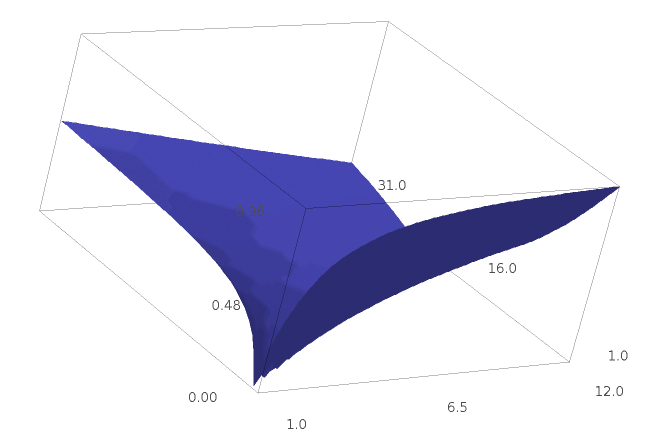
\includegraphics[height=2in]{rcbday.jpg}
          \end{center}
        \item We want to maximize this.
          \begin{equation*}
            \theta
            =
            \arccos(\,\frac{\colvec[r]{7 \\ 12}\dotprod\colvec{m \\ d}}{
                  \norm{\colvec[r]{7 \\ 12}\,}\cdot\norm{\colvec{m \\ d}\,} }\,)
          \end{equation*}
          Of course, we cannot take $m$ or $d$ negative and so we cannot
          get a vector orthogonal to the given one.
          This Python script finds the largest angle by brute force.
          \begin{verbatim}
  import math
  days={1:31,  # Jan
        2:29, 3:31, 4:30, 5:31, 6:30, 7:31, 8:31, 9:30, 10:31, 11:30, 12:31}
  BDAY=(7,12)
  max_res=0
  max_res_date=(-1,-1)
  for month in range(1,13):
      for day in range(1,days[month]+1):
          num=BDAY[0]*month+BDAY[1]*day
          denom=math.sqrt(BDAY[0]**2+BDAY[1]**2)*math.sqrt(month**2+day**2)
          if denom>0:
              res=math.acos(min(num*1.0/denom,1))
              print "day:",str(month),str(day)," angle:",str(res)
              if res>max_res:
                  max_res=res
                  max_res_date=(month,day)
  print "For ",str(BDAY),"the worst case is",str(max_res),"radians on date",str(max_res_date)
  print "  That is ",180*max_res/math.pi,"degrees"
          \end{verbatim}
          The result is
          \begin{verbatim}
  For  (7, 12) the worst case is 0.95958064648 radians on date (12, 1)
    That is  54.9799211457 degrees
\end{verbatim}

          A more conceptual approach is to consider the relation of all points
          $(\text{month},\text{day})$ to the point $(7,12)$.
          The picture below
          makes clear that the answer is either Dec~$1$ or Jan~$31$, depending
          on which is further from the birthdate.
          The dashed line bisects the angle between the line from the
          origin to Dec~$1$, and the line from the origin to Jan~$31$.
          Birthdays above the line are furthest from Dec~$1$ and
          birthdays below the line are furthest from Jan~$31$.
          \begin{center}
            \includegraphics{ch1.54}
          \end{center}
      \end{exparts}
    
\end{ans}
\begin{ans}{One.II.2.41}
      \answerasgiven %
      The actual velocity \( \vec{v} \) of the wind is the sum of the
      ship's velocity and the apparent velocity of the wind.
      Without loss of generality we may assume \( \vec{a} \) and
      \( \vec{b} \) to be unit vectors, and may write
      \begin{equation*}
         \vec{v}=\vec{v}_1+s\vec{a}=\vec{v}_2+t\vec{b}
      \end{equation*}
      where \( s \) and \( t \) are undetermined scalars.
      Take the dot product first by \( \vec{a} \) and then by \( \vec{b} \)
      to obtain
      \begin{align*}
         s-t\vec{a}\dotprod\vec{b}
         &=\vec{a}\dotprod(\vec{v}_2-\vec{v}_1)    \\
         s\vec{a}\dotprod\vec{b}-t
         &=\vec{b}\dotprod(\vec{v}_2-\vec{v}_1)
      \end{align*}
      Multiply the second by \( \vec{a}\dotprod\vec{b} \),
      subtract the result from the first, and find
      \begin{equation*}
         s=
         \frac{[\vec{a}-(\vec{a}\dotprod\vec{b})\vec{b}]
                   \dotprod(\vec{v}_2-\vec{v}_1)
              }{1-(\vec{a}\dotprod\vec{b})^2}.
      \end{equation*}
      Substituting in the original displayed equation, we get
      \begin{equation*}
         \vec{v}=\vec{v}_1+
         \frac{[\vec{a}-(\vec{a}\dotprod\vec{b})\vec{b}]
                  \dotprod(\vec{v}_2-\vec{v}_1)
              \vec{a}}{1-(\vec{a}\dotprod\vec{b})^2}.
      \end{equation*}
    
\end{ans}
\begin{ans}{One.II.2.42}
       We use induction on \( n \).

       In the \( n=1 \) base case the identity reduces to
       \begin{equation*}
          (a_1b_1)^2=({a_1}^2)({b_1}^2)-0
       \end{equation*}
       and clearly holds.

       For the inductive step assume that
       the formula holds for the \( 0 \), \ldots, \( n \) cases.
       We will show that it then holds in the \( n+1 \) case.
       Start with the right-hand side
       \begin{multline*}
         \bigl( \sum_{1\leq j\leq n+1}{a_j}^2\bigr)
         \bigl( \sum_{1\leq j\leq n+1}{b_j}^2\bigr)
         -
         \sum_{1\leq k<j\leq n+1}\bigl(a_kb_j-a_jb_k\bigr)^2  \\
       \begin{aligned}
         &=
         \bigl[ (\sum_{1\leq j\leq n}{a_j}^2)+{a_{n+1}}^2\bigr]
         \bigl[ (\sum_{1\leq j\leq n}{b_j}^2)+{b_{n+1}}^2\bigr]   \\
         &\hbox{}\quad -
         \bigl[\sum_{1\leq k<j\leq n}\bigl(a_kb_j-a_jb_k\bigr)^2+
         \sum_{1\leq k\leq n}\bigl(a_kb_{n+1}-a_{n+1}b_k\bigr)^2  \bigr] \\
         &=
         \bigl( \sum_{1\leq j\leq n}{a_j}^2\bigr)
         \bigl( \sum_{1\leq j\leq n}{b_j}^2\bigr)
         +
         \sum_{1\leq j\leq n}{b_j}^2{a_{n+1}}^2
         +
         \sum_{1\leq j\leq n}{a_j}^2{b_{n+1}}^2
         +
         {a_{n+1}}^2{b_{n+1}}^2                                 \\
         &\hbox{}\qquad\hbox{} -
         \bigl[\sum_{1\leq k<j\leq n}\bigl(a_kb_j-a_jb_k\bigr)^2+
         \sum_{1\leq k\leq n}\bigl(a_kb_{n+1}-a_{n+1}b_k\bigr)^2  \bigr] \\
         &=
         \bigl( \sum_{1\leq j\leq n}{a_j}^2\bigr)
         \bigl( \sum_{1\leq j\leq n}{b_j}^2\bigr)
         -\sum_{1\leq k<j\leq n}\bigl(a_kb_j-a_jb_k\bigr)^2   \\
         &\hbox{}\quad +
         \sum_{1\leq j\leq n}{b_j}^2{a_{n+1}}^2
         +
         \sum_{1\leq j\leq n}{a_j}^2{b_{n+1}}^2
         +
         {a_{n+1}}^2{b_{n+1}}^2                                 \\
         &\hbox{}\qquad\hbox{} -
         \sum_{1\leq k\leq n}\bigl(a_kb_{n+1}-a_{n+1}b_k\bigr)^2
        \end{aligned}
       \end{multline*}
       and apply the inductive hypothesis
       \begin{align*}
         &=
         \bigl( \sum_{1\leq j\leq n}a_jb_j\bigr)^2
         +
         \sum_{1\leq j\leq n}{b_j}^2{a_{n+1}}^2
         +
         \sum_{1\leq j\leq n}{a_j}^2{b_{n+1}}^2
         +
         {a_{n+1}}^2{b_{n+1}}^2                          \\
         &\hbox{}\qquad\hbox{}-
         \bigl[\sum_{1\leq k\leq n}{a_k}^2{b_{n+1}}^2
           -2\sum_{1\leq k\leq n}a_kb_{n+1}a_{n+1}b_k
           +\sum_{1\leq k\leq n}{a_{n+1}}^2{b_k}^2\bigr]        \\
         &=
         \bigl( \sum_{1\leq j\leq n}a_jb_j\bigr)^2
         +2\bigl(\sum_{1\leq k\leq n}a_kb_{n+1}a_{n+1}b_k\bigr)
         +{a_{n+1}}^2{b_{n+1}}^2                                 \\
         &=
         \bigl[\bigl(\sum_{1\leq j\leq n}a_jb_j\bigr)+a_{n+1}b_{n+1}\bigr]^2
       \end{align*}
       to derive the left-hand side.
   
\end{ans}
\section{Reduced Echelon Form}
\subsection{One.III.1: Gauss-Jordan Reduction}
\begin{ans}{One.III.1.8}
       These answers show only the Gauss-Jordan reduction.
       With it, describing the solution set is easy.
       \begin{exparts}
         \partsitem $\begin{amat}[r]{2}
               1  &1  &2  \\
               1  &-1 &0
             \end{amat}
             \grstep{-\rho_1+\rho_2}
             \begin{amat}[r]{2}
               1  &1  &2  \\
               0  &-2 &-2
             \end{amat}
             \grstep{-(1/2)\rho_2}
             \begin{amat}[r]{2}
               1  &1  &2  \\
               0  &1  &1
             \end{amat}
             \grstep{-\rho_2+\rho_1}
             \begin{amat}[r]{2}
               1  &0  &1  \\
               0  &1  &1
             \end{amat}$
         \partsitem $
             \begin{amat}[r]{3}
               1  &0  &-1  &4  \\
               2  &2  &0   &1
             \end{amat}
             \grstep{-2\rho_1+\rho_2}
             \begin{amat}[r]{3}
               1  &0  &-1  &4  \\
               0  &2  &2   &-7
             \end{amat}
             \grstep{(1/2)\rho_2}
             \begin{amat}[r]{3}
               1  &0  &-1  &4  \\
               0  &1  &1   &-7/2
             \end{amat}$
         \partsitem
           \begin{equation*}
             \begin{amat}[r]{2}
               3  &-2  &1  \\
               6  &1   &1/2
             \end{amat}
             \grstep{-2\rho_1+\rho_2}
             \begin{amat}[r]{2}
               3  &-2  &1  \\
               0  &5   &-3/2
             \end{amat}
             \grstep[(1/5)\rho_2]{(1/3)\rho_1}
             \begin{amat}[r]{2}
               1  &-2/3&1/3 \\
               0  &1   &-3/10
             \end{amat}
             \grstep{(2/3)\rho_2+\rho_1}
             \begin{amat}[r]{2}
               1  &0   &2/15 \\
               0  &1   &-3/10
             \end{amat}
          \end{equation*}
        \partsitem A row swap here makes the arithmetic easier.
         \begin{multline*}
          \begin{amat}[r]{3}
            2  &-1  &0  &-1  \\
            1  &3   &-1 &5   \\
            0  &1   &2  &5
          \end{amat}
          \grstep{-(1/2)\rho_1+\rho_2}
          \begin{amat}[r]{3}
            2  &-1  &0  &-1   \\
            0  &7/2 &-1 &11/2 \\
            0  &1   &2  &5
          \end{amat}
          \grstep{\rho_2\leftrightarrow\rho_3}
          \begin{amat}[r]{3}
            2  &-1  &0  &-1   \\
            0  &1   &2  &5    \\
            0  &7/2 &-1 &11/2
          \end{amat}                   \\
          \begin{aligned}
            &\grstep{-(7/2)\rho_2+\rho_3}
            \begin{amat}[r]{3}
              2  &-1  &0  &-1   \\
              0  &1   &2  &5    \\
              0  &0   &-8 &-12
            \end{amat}
            \grstep[-(1/8)\rho_2]{(1/2)\rho_1}
            \begin{amat}[r]{3}
              1  &-1/2&0  &-1/2 \\
              0  &1   &2  &5    \\
              0  &0   &1  &3/2
            \end{amat}                     \\
            &\grstep{-2\rho_3+\rho_2}
            \begin{amat}[r]{3}
              1  &-1/2&0  &-1/2 \\
              0  &1   &0  &2    \\
              0  &0   &1  &3/2
            \end{amat}
            \grstep{(1/2)\rho_2+\rho_1}
            \begin{amat}[r]{3}
              1  &0   &0  &1/2  \\
              0  &1   &0  &2    \\
              0  &0   &1  &3/2
            \end{amat}
          \end{aligned}
        \end{multline*}
       \end{exparts}
     
\end{ans}
\begin{ans}{One.III.1.9}
      Use Gauss-Jordan reduction.
      \begin{exparts}
        \partsitem $
            \grstep{-(1/2)\rho_1+\rho_2}
            \begin{mat}[r]
              2  &1  \\
              0  &5/2
            \end{mat}
            \grstep[(2/5)\rho_2]{(1/2)\rho_1}
            \begin{mat}[r]
              1  &1/2\\
              0  &1
            \end{mat}
            \grstep{-(1/2)\rho_2+\rho_1}
            \begin{mat}[r]
              1  &0  \\
              0  &1
            \end{mat}$
        \partsitem $
            \grstep[\rho_1+\rho_3]{-2\rho_1+\rho_2}
            \begin{mat}[r]
              1  &3  &1  \\
              0  &-6 &2  \\
              0  &0  &-2
            \end{mat}
            \grstep[-(1/2)\rho_3]{-(1/6)\rho_2}
            \begin{mat}[r]
              1  &3  &1     \\
              0  &1  &-1/3  \\
              0  &0  &1
            \end{mat}
            \grstep[-\rho_3+\rho_1]{(1/3)\rho_3+\rho_2}
            \begin{mat}[r]
              1  &3  &0     \\
              0  &1  &0     \\
              0  &0  &1
            \end{mat}
            \grstep{-3\rho_2+\rho_1}
            \begin{mat}[r]
              1  &0  &0     \\
              0  &1  &0     \\
              0  &0  &1
            \end{mat}$
        \partsitem \ \begin{multline*}
            \grstep[-3\rho_1+\rho_3]{-\rho_1+\rho_2}
            \begin{mat}[r]
              1  &0  &3  &1  &2  \\
              0  &4  &-1 &0  &3  \\
              0  &4  &-1 &-2 &-4
            \end{mat}
            \grstep{-\rho_2+\rho_3}
            \begin{mat}[r]
              1  &0  &3  &1  &2  \\
              0  &4  &-1 &0  &3  \\
              0  &0  &0  &-2 &-7
            \end{mat}                           \\
            \grstep[-(1/2)\rho_3]{(1/4)\rho_2}
            \begin{mat}[r]
              1  &0  &3    &1  &2  \\
              0  &1  &-1/4 &0  &3/4  \\
              0  &0  &0    &1  &7/2
            \end{mat}
            \grstep{-\rho_3+\rho_1}
            \begin{mat}[r]
              1  &0  &3    &0  &-3/2  \\
              0  &1  &-1/4 &0  &3/4     \\
              0  &0  &0    &1  &7/2
            \end{mat}
          \end{multline*}
        \partsitem \ \begin{multline*}
            \grstep{\rho_1\leftrightarrow\rho_3}
            \begin{mat}[r]
              1  &5  &1  &5  \\
              0  &0  &5  &6  \\
              0  &1  &3  &2
            \end{mat}
            \grstep{\rho_2\leftrightarrow\rho_3}
            \begin{mat}[r]
              1  &5  &1  &5  \\
              0  &1  &3  &2  \\
              0  &0  &5  &6
            \end{mat}
            \grstep{(1/5)\rho_3}
            \begin{mat}[r]
              1  &5  &1  &5  \\
              0  &1  &3  &2  \\
              0  &0  &1  &6/5
            \end{mat}                  \\
            \grstep[-\rho_3+\rho_1]{-3\rho_3+\rho_2}
            \begin{mat}[r]
              1  &5  &0  &19/5  \\
              0  &1  &0  &-8/5  \\
              0  &0  &1  &6/5
            \end{mat}
            \grstep{-5\rho_2+\rho_1}
            \begin{mat}[r]
              1  &0  &0  &59/5  \\
              0  &1  &0  &-8/5  \\
              0  &0  &1  &6/5
            \end{mat}
          \end{multline*}
      \end{exparts}
    
\end{ans}
\begin{ans}{One.III.1.10}
      For the Gauss's halves, see the answers to Chapter One's
      section~I.2 question
      \nearbyexercise{exer:SlvMatNot}.
      \begin{exparts}
      \partsitem The ``Jordan'' half goes this way.
        \begin{equation*}
          \grstep[-(1/3)\rho_2]{(1/2)\rho_1}
          \begin{amat}[r]{3}
            1  &1/2 &-1/2 &1/2  \\
            0  &1   &-2/3 &-1/3
          \end{amat}
          \grstep{-(1/2)\rho_2+\rho_1}
          \begin{amat}[r]{3}
            1  &0   &-1/6 &2/3  \\
            0  &1   &-2/3 &-1/3
          \end{amat}
        \end{equation*}
        The solution set is this
        \begin{equation*}
          \set{\colvec[r]{2/3 \\ -1/3 \\ 0}
               +\colvec[r]{1/6 \\ 2/3 \\ 1}z
              \suchthat z\in\Re}
        \end{equation*}
      \partsitem The second half is
        \begin{equation*}
          \grstep{\rho_3+\rho_2}
          \begin{amat}[r]{4}
            1  &0  &-1  &0  &1 \\
            0  &1  &2   &0  &3 \\
            0  &0  &0   &1  &0
          \end{amat}
        \end{equation*}
        so the solution is this.
        \begin{equation*}
          \set{\colvec[r]{1 \\ 3 \\ 0 \\ 0}
               +\colvec[r]{1 \\ -2 \\ 1 \\ 0}z
              \suchthat z\in\Re}
        \end{equation*}
      \partsitem This Jordan half
        \begin{equation*}
          \grstep{\rho_2+\rho_1}
          \begin{amat}[r]{4}
            1  &0  &1   &1  &0 \\
            0  &1  &0   &1  &0 \\
            0  &0  &0   &0  &0 \\
            0  &0  &0   &0  &0
          \end{amat}
        \end{equation*}
        gives
        \begin{equation*}
          \set{\colvec[r]{0 \\ 0 \\ 0 \\ 0}
               +\colvec[r]{-1 \\ 0 \\ 1 \\ 0}z
               +\colvec[r]{-1 \\ -1 \\ 0 \\ 1}w
              \suchthat z,w\in\Re}
        \end{equation*}
        (of course, we could omit the zero vector from the description).
      \partsitem The ``Jordan'' half
        \begin{equation*}
          \grstep{-(1/7)\rho_2}
          \begin{amat}[r]{5}
            1  &2  &3   &1   &-1   &1  \\
            0  &1  &8/7 &2/7 &-4/7 &0
          \end{amat}
          \grstep{-2\rho_2+\rho_1}
          \begin{amat}[r]{5}
            1  &0  &5/7 &3/7 &1/7  &1  \\
            0  &1  &8/7 &2/7 &-4/7 &0
          \end{amat}
        \end{equation*}
        ends with this solution set.
        \begin{equation*}
          \set{\colvec[r]{1 \\ 0 \\ 0 \\ 0 \\ 0}
               +\colvec[r]{-5/7 \\ -8/7 \\ 1 \\ 0 \\ 0}c
               +\colvec[r]{-3/7 \\ -2/7 \\ 0 \\ 1 \\ 0}d
               +\colvec[r]{-1/7 \\ 4/7 \\ 0 \\ 0 \\ 1}e
              \suchthat c,d,e\in\Re}
        \end{equation*}
    \end{exparts}
   
\end{ans}
\begin{ans}{One.III.1.11}
      Routine Gauss's Method gives one:
      \begin{equation*}
        \grstep[-(1/2)\rho_1+\rho_3]{-3\rho_1+\rho_2}
        \begin{mat}[r]
          2  &1  &1  &3  \\
          0  &1  &-2 &-7 \\
          0  &9/2&1/2&7/2
        \end{mat}
        \grstep{-(9/2)\rho_2+\rho_3}
        \begin{mat}[r]
          2  &1  &1    &3  \\
          0  &1  &-2   &-7 \\
          0  &0  &19/2 &35
        \end{mat}
      \end{equation*}
      and any cosmetic change, like multiplying the bottom row by \( 2 \),
      \begin{equation*}
        \begin{mat}[r]
          2  &1  &1    &3  \\
          0  &1  &-2   &-7 \\
          0  &0  &19   &70
        \end{mat}
      \end{equation*}
      gives another.
    
\end{ans}
\begin{ans}{One.III.1.12}
      In the cases listed below, we take $a,b\in\Re$.
      Thus, some canonical forms
      listed below actually include infinitely many cases.
      In particular, they includes the cases $a=0$ and $b=0$.
      \begin{exparts}
        \partsitem
          $\begin{mat}[r]
            0  &0  \\
            0  &0
          \end{mat}$,
          $\begin{mat}[r]
            1  &a  \\
            0  &0
          \end{mat}$,
          $\begin{mat}[r]
            0  &1  \\
            0  &0
          \end{mat}$,
          $\begin{mat}[r]
            1  &0  \\
            0  &1
          \end{mat}$
        \partsitem
          $\begin{mat}[r]
               0  &0  &0  \\
               0  &0  &0
             \end{mat}$,
          $\begin{mat}[r]
               1  &a  &b  \\
               0  &0  &0
             \end{mat}$,
          $\begin{mat}[r]
               0  &1  &a  \\
               0  &0  &0
             \end{mat}$,
          $\begin{mat}[r]
               0  &0  &1  \\
               0  &0  &0
             \end{mat}$,
          $\begin{mat}[r]
               1  &0  &a  \\
               0  &1  &b
             \end{mat}$,
          $\begin{mat}[r]
               1  &a  &0  \\
               0  &0  &1
             \end{mat}$,
          $\begin{mat}[r]
               0  &1  &0  \\
               0  &0  &1
             \end{mat}$
        \partsitem
          $\begin{mat}[r]
               0  &0  \\
               0  &0  \\
               0  &0
             \end{mat}$,
          $\begin{mat}[r]
               1  &a  \\
               0  &0  \\
               0  &0
             \end{mat}$,
          $\begin{mat}[r]
               0  &1  \\
               0  &0  \\
               0  &0
             \end{mat}$,
          $\begin{mat}[r]
               1  &0  \\
               0  &1  \\
               0  &0
             \end{mat}$
        \partsitem
          $\begin{mat}[r]
               0  &0  &0  \\
               0  &0  &0  \\
               0  &0  &0
             \end{mat}$,
          $\begin{mat}[r]
               1  &a  &b  \\
               0  &0  &0  \\
               0  &0  &0
             \end{mat}$,
          $\begin{mat}[r]
               0  &1  &a  \\
               0  &0  &0  \\
               0  &0  &0
             \end{mat}$,
          $\begin{mat}[r]
               0  &0  &1  \\
               0  &0  &0  \\
               0  &0  &0
             \end{mat}$,
          $\begin{mat}[r]
               1  &0  &a  \\
               0  &1  &b  \\
               0  &0  &0
             \end{mat}$,
          $\begin{mat}[r]
               1  &a  &0  \\
               0  &0  &1  \\
               0  &0  &0
             \end{mat}$,
          $\begin{mat}[r]
               1  &0  &0  \\
               0  &1  &0  \\
               0  &0  &1
             \end{mat}$
      \end{exparts}
    
\end{ans}
\begin{ans}{One.III.1.13}
      A nonsingular homogeneous linear system has a unique solution.
      So a nonsingular matrix must reduce to a (square)
      matrix that is all \( 0 \)'s
      except for \( 1 \)'s down the upper-left to lower-right diagonal, e.g.,
      \begin{equation*}
         \begin{mat}[r]
           1  &0  \\
           0  &1  \\
         \end{mat},
         \quad\text{or}\quad
         \begin{mat}[r]
           1  &0  &0  \\
           0  &1  &0  \\
           0  &0  &1
         \end{mat},
         \quad\text{etc.}
      \end{equation*}
    
\end{ans}
\begin{ans}{One.III.1.14}
      It is an equivalence relation.
      To prove that we must check that the relation
      is reflexive, symmetric, and transitive.

      Assume that all matrices are $\nbyn{2}$.
      For reflexive, we note that a matrix has the same sum of entries as
      itself.
      For symmetric, we assume $A$ has the same sum of entries as~$B$
      and obviously then $B$ has the same sum of entries as~$A$.
      Transitivity is no harder\Dash if $A$ has the same sum of entries
      as $B$ and $B$ has the same sum of entries as $C$ then
      $A$ has the same as $C$.
    
\end{ans}
\begin{ans}{One.III.1.15}
    \begin{exparts}
      \partsitem The $\rho_i\leftrightarrow\rho_i$ operation does not
        change $A$.
      \partsitem For instance,
        \begin{equation*}
          \begin{mat}[r]
            1  &2  \\
            3  &4
          \end{mat}
          \grstep{-\rho_1+\rho_1}
          \begin{mat}[r]
            0  &0  \\
            3  &4
          \end{mat}
          \grstep{\rho_1+\rho_1}
          \begin{mat}[r]
            0  &0  \\
            3  &4
          \end{mat}
        \end{equation*}
        leaves the matrix changed.
      \partsitem If $i\neq j$ then
        \begin{eqnarray*}
          \begin{mat}
            \vdotswithin{a_{i,1}}                     \\
            a_{i,1}  &\cdots  &a_{i,n}  \\
            \vdotswithin{a_{i,1}}                     \\
            a_{j,1}  &\cdots  &a_{j,n}  \\
            \vdotswithin{a_{i,1}}
          \end{mat}
          &\grstep{k\rho_i+\rho_j}
          &\begin{mat}
            \vdotswithin{a_{i,1}}                                      \\
            a_{i,1}           &\cdots  &a_{i,n}          \\
            \vdotswithin{a_{i,1}}                                      \\
            ka_{i,1}+a_{j,1}  &\cdots  &ka_{i,n}+a_{j,n}  \\
            \vdotswithin{a_{i,1}}
          \end{mat}                                        \\
          &\grstep{-k\rho_i+\rho_j}
          &\begin{mat}
            \vdotswithin{a_{i,1}}                                      \\
            a_{i,1}           &\cdots  &a_{i,n}          \\
            \vdotswithin{a_{i,1}}                                      \\
            -ka_{i,1}+ka_{i,1}+a_{j,1}  &\cdots &-ka_{i,n}+ka_{i,n}+a_{j,n} \\
            \vdotswithin{a_{i,1}}
          \end{mat}
        \end{eqnarray*}
        does indeed give $A$ back.
        (Of course, if $i=j$ then the third matrix would have entries of the
        form $-k(ka_{i,j}+a_{i,j})+ka_{i,j}+a_{i,j}$.)
    \end{exparts}
   
\end{ans}
\begin{ans}{One.III.1.16}
    To be an equivalence, each relation must be reflexive, symmetric, and
    transitive.
    \begin{exparts}
      \item This relation
        is not symmetric because if $x$ has taken $4$~classes and $y$
        has taken $3$ then $x$ is related to $y$ but $y$ is not related
        to $x$.
      \item This is reflexive because $x$'s name starts with the same
        letter as does $x$'s.
        It is symmetric because if $x$'s name starts with the same letter
        as $y$'s then $y$'s starts with the same letter as does~$x$'s.
        And it is transitive because if $x$'s name starts with the same letter
        as does~$y$'s and $y$'s name starts with the same letter as
        does $z$'s then $x$'s starts with the same letter as does $z$'s.
        So it is an equivalence.
    \end{exparts}
  
\end{ans}
\begin{ans}{One.III.1.17}
    For each we must check the three conditions of reflexivity, symmetry, and
    transitivity.
    \begin{exparts}
      \item Any matrix clearly has the same product down the diagonal as
        itself, so the relation is reflexive.
        The relation is symmetric because if $A$ has the same product down
        its diagonal as does~$B$,
        if $a_{1,1}\cdot a_{2,2}=b_{1,1}\cdot b_{2,2}$,
        then $B$ has the same product as does~$A$.

        Transitivity is similar: suppose that $A$'s product is~$r$ and
        that it equals $B$'s product.
        Suppose also that $B$'s product equals $C$'s.
        Then all three have a product of~$r$, and $A$'s equals~$C$'s.

        There is an equivalence class for each real number, namely the
        class contains all $\nbyn{2}$ matrices whose product down the
        diagonal is that real.
      \item For reflexivity, if the matrix $A$ has a~$1$ entry then it is
        related to itself while if it does not then it is also related to
        itself.
        Symmetry also has two cases: suppose that $A$ and~$B$ are related.
        If $A$ has a~$1$ entry then so does~$B$, and thus $B$ is related to~$A$.
        If $A$ has no~$1$ then neither does $B$, and again $B$ is related to
        $A$.

        For transitivity, suppose that $A$ is related to~$B$ and $B$ to~$C$.
        If $A$ has a~$1$ entry then so does~$B$, and because $B$ is related
        to~$C$, therefore so does~$C$,
        and hence $A$ is related to~$C$.
        Likewise, if $A$ has no~$1$ then neither does~$B$, and consequently
        neither does~$C$, giving the conclusion that $A$ is related to~$C$.

        There are exactly two equivalence classes, one containing any
        $\nbyn{2}$ matrix that has at least one entry that is a~$1$,
        and the other containing all the matrices that have no $1$'s.
    \end{exparts}
  
\end{ans}
\begin{ans}{One.III.1.18}
      \begin{exparts}
        \item This relation is not reflexive.
          For instance, any matrix with an upper-left entry of~$1$ is not
          related to itself.
        \item This relation is not transitive.
          For these three, $A$ is related to~$B$, and $B$ is related to~$C$,
          but $A$ is not related to~$C$.
          \begin{equation*}
            A=\begin{mat}
              0 &0 \\
              0 &0
            \end{mat},\quad
            B=\begin{mat}
              4 &0 \\
              0 &0
            \end{mat},\quad
            C=\begin{mat}
              8 &0 \\
              0 &0
            \end{mat},\quad
          \end{equation*}
      \end{exparts}
    
\end{ans}
\subsection{One.III.2: The Linear Combination Lemma}
\begin{ans}{One.III.2.10}
      Bring each to reduced echelon form and compare.
      \begin{exparts}
        \partsitem The first gives
          \begin{equation*}
            \grstep{-4\rho_1+\rho_2}
            \begin{mat}[r]
              1  &2  \\
              0  &0
            \end{mat}
          \end{equation*}
          while the second gives
          \begin{equation*}
            \grstep{\rho_1\leftrightarrow\rho_2}
            \begin{mat}[r]
              1  &2  \\
              0  &1
            \end{mat}
            \grstep{-2\rho_2+\rho_1}
            \begin{mat}[r]
              1  &0  \\
              0  &1
            \end{mat}
          \end{equation*}
          The two reduced echelon form matrices are not identical, and so the
          original matrices are not row equivalent.
        \partsitem The first is this.
          \begin{equation*}
            \grstep[-5\rho_1+\rho_3]{-3\rho_1+\rho_2}
            \begin{mat}[r]
              1  &0  &2  \\
              0  &-1 &-5 \\
              0  &-1 &-5
            \end{mat}
            \grstep{-\rho_2+\rho_3}
            \begin{mat}[r]
              1  &0  &2  \\
              0  &-1 &-5 \\
              0  &0  &0
            \end{mat}
            \grstep{-\rho_2}
            \begin{mat}[r]
              1  &0  &2  \\
              0  &1  &5  \\
              0  &0  &0
            \end{mat}
          \end{equation*}
          The second is this.
          \begin{equation*}
            \grstep{-2\rho_1+\rho_3}
            \begin{mat}[r]
              1  &0  &2  \\
              0  &2  &10 \\
              0  &0  &0
            \end{mat}
            \grstep{(1/2)\rho_2}
            \begin{mat}[r]
              1  &0  &2  \\
              0  &1  &5  \\
              0  &0  &0
            \end{mat}
          \end{equation*}
          These two are row equivalent.
        \partsitem These two are not row equivalent because they have different
          sizes.
        \partsitem The first,
          \begin{equation*}
            \grstep{\rho_1+\rho_2}
            \begin{mat}[r]
              1  &1  &1  \\
              0  &3  &3
            \end{mat}
            \grstep{(1/3)\rho_2}
            \begin{mat}[r]
              1  &1  &1  \\
              0  &1  &1
            \end{mat}
            \grstep{-\rho_2+\rho_1}
            \begin{mat}[r]
              1  &0  &0  \\
              0  &1  &1
            \end{mat}
          \end{equation*}
          and the second.
          \begin{equation*}
            \grstep{\rho_1\leftrightarrow\rho_2}
            \begin{mat}[r]
              2  &2  &5  \\
              0  &3  &-1
            \end{mat}
            \grstep[(1/3)\rho_2]{(1/2)\rho_1}
            \begin{mat}[r]
              1  &1  &5/2 \\
              0  &1  &-1/3
            \end{mat}
            \grstep{-\rho_2+\rho_1}
            \begin{mat}[r]
              1  &0  &17/6 \\
              0  &1  &-1/3
            \end{mat}
          \end{equation*}
          These are not row equivalent.
        \partsitem Here the first is
          \begin{equation*}
            \grstep{(1/3)\rho_2}
            \begin{mat}[r]
              1  &1  &1  \\
              0  &0  &1
            \end{mat}
            \grstep{-\rho_2+\rho_1}
            \begin{mat}[r]
              1  &1  &0  \\
              0  &0  &1
            \end{mat}
          \end{equation*}
          while this is the second.
          \begin{equation*}
            \grstep{\rho_1\leftrightarrow\rho_2}
            \begin{mat}[r]
              1  &-1 &1  \\
              0  &1  &2
            \end{mat}
            \grstep{\rho_2+\rho_1}
            \begin{mat}[r]
              1  &0  &3  \\
              0  &1  &2
            \end{mat}
          \end{equation*}
          These are not row equivalent.
       \end{exparts}
     
\end{ans}
\begin{ans}{One.III.2.11}
       First, the only matrix row equivalent to the matrix of all
       \( 0 \)'s is itself (since row operations have no effect).

       Second, the matrices that reduce to
       \begin{equation*}
         \begin{mat}
           1  &a  \\
           0  &0
         \end{mat}
       \end{equation*}
       have the form
       \begin{equation*}
         \begin{mat}
           b  &ba \\
           c  &ca
         \end{mat}
       \end{equation*}
       (where \( a,b,c\in\Re \), and \(b\) and \(c\) are not both zero).

       Next, the matrices that reduce to
       \begin{equation*}
         \begin{mat}[r]
           0  &1  \\
           0  &0
         \end{mat}
       \end{equation*}
       have the form
       \begin{equation*}
         \begin{mat}
           0  &a \\
           0  &b
         \end{mat}
       \end{equation*}
       (where \( a,b\in\Re \), and not both are zero).

       Finally, the matrices that reduce to
       \begin{equation*}
         \begin{mat}[r]
           1  &0  \\
           0  &1
         \end{mat}
       \end{equation*}
       are the nonsingular matrices.
       That's because a linear system for which this is the matrix of
       coefficients will have a unique solution, and that is the definition
       of nonsingular.
       (Another way to say the same thing is to say that they fall into none
       of the above classes.)
     
\end{ans}
\begin{ans}{One.III.2.12}
      \begin{exparts}
        \partsitem They have the form
          \begin{equation*}
            \begin{mat}
              a  &0  \\
              b  &0
            \end{mat}
          \end{equation*}
          where \( a,b\in\Re \).
        \partsitem They have this form (for \( a,b\in\Re \)).
          \begin{equation*}
            \begin{mat}
             1a  &2a \\
             1b  &2b
            \end{mat}
          \end{equation*}
        \partsitem They have the form
          \begin{equation*}
            \begin{mat}
              a  &b  \\
              c  &d
            \end{mat}
          \end{equation*}
          (for \( a,b,c,d\in\Re \)) where \( ad-bc\neq 0 \).
          (This is the formula that determines when a \( \nbyn{2} \) matrix
          is nonsingular.)
      \end{exparts}
    
\end{ans}
\begin{ans}{One.III.2.13}
       Infinitely many.
       For instance, in
       \begin{equation*}
         \begin{mat}
           1  &k  \\
           0  &0
         \end{mat}
       \end{equation*}
       each $k\in\Re$ gives a different class.
    
\end{ans}
\begin{ans}{One.III.2.14}
      No.
      Row operations do not change the size of a matrix.
    
\end{ans}
\begin{ans}{One.III.2.15}
     \begin{exparts}
      \partsitem A row operation on a matrix of zeros has no effect.
        Thus each such matrix is alone in its row equivalence class.
      \partsitem No.
        Any nonzero entry can be rescaled.
     \end{exparts}
    
\end{ans}
\begin{ans}{One.III.2.16}
      Here are two.
      \begin{equation*}
        \begin{mat}[r]
          1  &1  &0  \\
          0  &0  &1
        \end{mat}
        \quad\text{and}\quad
        \begin{mat}[r]
          1  &0  &0  \\
          0  &0  &1
        \end{mat}
      \end{equation*}
     
\end{ans}
\begin{ans}{One.III.2.17}
      Any two \( \nbyn{n} \) nonsingular matrices have
      the same reduced echelon
      form, namely the matrix with all \( 0 \)'s except for \( 1 \)'s down
      the diagonal.
      \begin{equation*}
        \begin{mat}
          1  &0  &       &0  \\
          0  &1  &       &0  \\
             &   &\ddots &   \\
          0  &0  &       &1
        \end{mat}
      \end{equation*}

      Two same-sized singular matrices need not be row equivalent.
      For example, these two \( \nbyn{2} \) singular matrices
      are not row equivalent.
      \begin{equation*}
        \begin{mat}[r]
          1  &1  \\
          0  &0
        \end{mat}
        \quad\text{and}\quad
        \begin{mat}[r]
          1  &0  \\
          0  &0
        \end{mat}
      \end{equation*}
    
\end{ans}
\begin{ans}{One.III.2.18}
      Since there is one and only one reduced echelon form matrix in each
      class, we can just list the possible reduced echelon form matrices.

      For that list, see the answer for \nearbyexercise{exer:PossRedEchFrms}.
    
\end{ans}
\begin{ans}{One.III.2.19}
          \begin{exparts}
           \partsitem If there is a linear relationship where $c_0$ is not zero
             then we can subtract $c_0\vec{\beta}_0$ from both sides and divide
             by $-c_0$ to get $\vec{\beta}_0$ as a linear
             combination of the others.
             (Remark:
             if there are no other vectors in the set\Dash if the
             relationship is, say,
             $\zero=3\cdot\zero$\Dash then the statement is still true because
             the zero vector is by definition the sum of the empty set
             of vectors.)

             Conversely, if $\vec{\beta}_0$ is a combination of the others
             $\vec{\beta}_0=c_1\vec{\beta}_1+\dots+c_n\vec{\beta}_n$
             then subtracting
             $\vec{\beta}_0$ from both sides gives a relationship where
             at least one
             of the coefficients is nonzero; namely,
             the $-1$ in front of $\vec{\beta}_0$.
           \partsitem The first row is not a linear combination of the
             others for
             the reason given in the proof:~in the equation of components from
             the column containing the leading entry of the first row, the
             only nonzero entry is the leading entry from the first row, so
             its coefficient must be zero.
             Thus, from the prior part of this exercise, the first row is in
             no linear relationship with the other rows.

             Thus, when considering whether the second row can be in a linear
             relationship
             with the other rows, we can leave the first row out.
             But now the argument just applied to the first row will apply
             to the second row.
             (That is, we are arguing here by induction.)
         \end{exparts}
      
\end{ans}
\begin{ans}{One.III.2.20}
     We know that $4s+c+10d=8.45$ and that $3s+c+7d=6.30$, and we'd like to
     know what $s+c+d$ is.
     Fortunately, $s+c+d$ is a linear combination of $4s+c+10d$ and $3s+c+7d$.
     Calling the unknown price $p$, we have this reduction.
     \begin{equation*}
       \begin{amat}{3}
         4  &1  &10  &8.45 \\
         3  &1  &7   &6.30 \\
         1  &1  &1   &p
       \end{amat}
       \grstep[-(1/4)\rho_1+\rho_3]{-(3/4)\rho_1+\rho_2}
       \begin{amat}{3}
         4  &1    &10     &8.45      \\
         0  &1/4  &-1/2   &-0.037\,5 \\
         0  &3/4  &-3/2   &p-2.112\,5
       \end{amat}
       \grstep{-3\rho_2+\rho_3}
       \begin{amat}{3}
         4  &1    &10     &8.45      \\
         0  &1/4  &-1/2   &-0.037\,5 \\
         0  &0    &0      &p-2.00
       \end{amat}
     \end{equation*}
     The price paid is \$$2.00$.
   
\end{ans}
\begin{ans}{One.III.2.21}
     \begin{enumerate}
        \item An easy answer is this:
          \begin{equation*}
            0=3.
          \end{equation*}
          For a less wise-guy-ish answer, solve the system:
          \begin{equation*}
            \begin{amat}[r]{2}
              3  &-1  &8  \\
              2  &1   &3
            \end{amat}
            \grstep{-(2/3)\rho_1+\rho_2}
            \begin{amat}[r]{2}
              3  &-1  &8    \\
              0  &5/3 &-7/3
            \end{amat}
          \end{equation*}
          gives \( y=-7/5 \) and \( x=11/5 \).
          Now any equation not satisfied by \( (-7/5,11/5) \) will do,
          e.g., \( 5x+5y=3 \).
        \item Every equation can be derived from an inconsistent system.
          For instance, here is how to derive ``\( 3x+2y=4 \)'' from
          ``\( 0=5 \)''.
          First,
          \begin{equation*}
            0=5
            \grstep{(3/5)\rho_1}
            0=3
            \grstep{x\rho_1}
            0=3x
          \end{equation*}
          (validity of the \( x=0 \) case is separate but clear).
          Similarly, \( 0=2y \).
          Ditto for \( 0=4 \).
          But now, \( 0+0=0 \) gives \( 3x+2y=4 \).
     \end{enumerate}
    
\end{ans}
\begin{ans}{One.III.2.22}
      Define linear systems to be equivalent if their augmented
      matrices are row equivalent.
      The proof that equivalent systems have the same solution set is easy.
    
\end{ans}
\begin{ans}{One.III.2.23}
      \begin{exparts}
        \partsitem The three possible row swaps are easy,
          as are the three possible rescalings.
          One of the six possible row combinations is \( k\rho_1+\rho_2 \):
          \begin{equation*}
            \begin{mat}
              1           &2           &3  \\
              k\cdot 1+3  &k\cdot 2+0  &k\cdot 3+3  \\
              1           &4           &5
            \end{mat}
          \end{equation*}
          and again the first and second columns add to the third.
          The other five combinations are similar.
        \partsitem The obvious conjecture is that row operations do not change
          linear relationships among columns.
        \partsitem A case-by-case
          proof follows the sketch given in the first item.
      \end{exparts}
   
\end{ans}
\topic{Computer Algebra Systems}
\begin{ans}{1}
      \begin{exparts}
        \partsitem The commands
\begin{indented}{\small
\begin{verbatim}
> A:=array( [[40,15],
             [-50,25]] );
> u:=array([100,50]);
> linsolve(A,u);
\end{verbatim}
}\end{indented}
           yield the answer $[1,4]$.
        \partsitem Here there is a free variable:
\begin{indented}{\small
\begin{verbatim}
> A:=array( [[7,0,-7,0],
             [8,1,-5,2],
             [0,1,-3,0],
             [0,3,-6,-1]] );
> u:=array([0,0,0,0]);
> linsolve(A,u);
\end{verbatim}
}\end{indented}
         prompts the reply $[\_t_1,3\_t_1,\_t_1,3\_t_1]$.
      \end{exparts}
    
\end{ans}
\begin{ans}{2}
      These are easy to type in.
      For instance, the first
\begin{indented}{\small
\begin{verbatim}
> A:=array( [[2,2],
             [1,-4]] );
> u:=array([5,0]);
> linsolve(A,u);
\end{verbatim}
}\end{indented}
      gives the expected answer of $[2,1/2]$.
      The others are similar.
      \begin{exparts}
        \partsitem The answer is \( x=2 \) and \( y=1/2 \).
        \partsitem The answer is \( x=1/2 \) and \( y=3/2 \).
        \partsitem This system has infinitely many solutions.
           In the first subsection, with $z$ as a parameter,
           we got $x=(43-7z)/4$ and $y=(13-z)/4$.
           Maple responds with $[-12+7\_t_1,\_t_1,13-4\_t_1]$,
           for some reason preferring $y$ as a parameter.
        \partsitem There is no solution to this system.
           When the array $A$ and vector $u$ are given to Maple
           and it is asked to \texttt{linsolve(A,u)},
           it returns no result at all, that is, it responds with
           no solutions.
        \partsitem The solutions is \( (x,y,z)=(5,5,0) \).
        \partsitem There are many solutions.
           Maple gives $[1,-1+\_t_1,3-\_t_1,\_t_1]$.
      \end{exparts}
    
\end{ans}
\begin{ans}{3}
      As with the prior question, entering these is easy.
      \begin{exparts}
        \partsitem This system has infinitely many solutions.
              In the second subsection we gave the solution set as
              \begin{equation*}
              \set{\colvec{6 \\ 0}+\colvec{-2 \\ 1}y
                      \suchthat y\in\Re}
              \end{equation*}
              and Maple responds with $[6-2\_t_1,\_t_1]$.
        \partsitem The solution set has only one member
          \begin{equation*}
             \set{\colvec{0 \\ 1} }
          \end{equation*}
          and Maple has no trouble finding it $[0,1]$.
        \partsitem This system's solution set is infinite
          \begin{equation*}
            \set{\colvec{4 \\ -1 \\ 0}+\colvec{-1 \\ 1 \\ 1}x_3
                             \suchthat x_3\in\Re}
          \end{equation*}
          and Maple gives $[\_t_1,-\_t_1+3,-\_t_1+4]$.
        \partsitem There is a unique solution
           \begin{equation*}
             \set{\colvec{1 \\ 1 \\ 1}}
           \end{equation*}
           and Maple gives $[1,1,1]$.
        \partsitem This system has infinitely many solutions; in the
           second subsection we described the solution set with
           two parameters
           \begin{equation*}
             \set{\colvec{5/3 \\ 2/3 \\ 0 \\ 0}
                  +\colvec{-1/3 \\ 2/3 \\ 1 \\ 0}z
                  +\colvec{-2/3 \\ 1/3 \\ 0 \\ 1}w
                  \suchthat z,w\in\Re}
           \end{equation*}
           as does Maple $[3-2\_t_1+\_t_2,\_t_1,\_t_2,-2+3\_t_1-2\_t_2]$.
        \partsitem The solution set is empty and Maple replies to the
           \texttt{linsolve(A,u)} command with no returned solutions.
      \end{exparts}
    
\end{ans}
\begin{ans}{4}
       In response to this prompting
\begin{indented}{\small
\begin{verbatim}
> A:=array( [[a,c],
             [b,d]] );
> u:=array([p,q]);
> linsolve(A,u);
\end{verbatim}
}\end{indented}
      Maple thought for perhaps twenty seconds and gave this reply.
      \begin{equation*}
        \bigl[-\frac{-d\,p+q\,c}{-b\,c+a\,d},
          \frac{-b\,p+a\,q}{-b\,c+a\,d}\bigr]
      \end{equation*}
    
\end{ans}
\topic{Input-Output Analysis}
\begin{ans}{1}
      These answers are from \textit{Octave}.
      \begin{exparts}
        \partsitem With the external use of steel as $17,789$ and the
          external use of autos as $21,243$ we get $s=25,952$, $a=30,312$.
        \partsitem $s=25,857$, $a=30,596$
        \partsitem $s=25,984$, $a=30,597$
      \end{exparts}
    
\end{ans}
\begin{ans}{2}
      This \textit{Sage} session
\begin{lstlisting}
sage: var('a,s')
(a, s)
sage: eqns=[(20053/25448)*s - (2664/30346)*a == 17589,
....:       (-48/25448)*s + (21316/30346)*a == 21243]
sage: solve(eqns, s, a)
[[s == (2745320544312/106830469), a == (6476293881123/213660938)]]
sage: s_by_s = (5395/25448)*2745320544312/106830469
sage: s_by_s
582010544505/106830469
sage: n(s_by_s)
5447.98267716114
sage: s_by_a = (2664/30346)*6476293881123/213660938
sage: n(s_by_a)
2660.93449955743
sage: a_by_s = (48/25448)*2745320544312/106830469
sage: n(a_by_s)
48.4713936058822
sage: a_by_a = (9030/30346)*6476293881123/213660938
sage: n(a_by_a)
9019.60905818451
\end{lstlisting}
      gives this table.
      \begin{center}
        \begin{tabular}{r|rrrr}
         \multicolumn{1}{c}{\ }  %put the | in the right place
         &\multicolumn{1}{r}{\begin{tabular}[b]{@{}c@{}}
                                \textit{used by} \\[-.65ex] \textit{steel}
                             \end{tabular}}
         &\multicolumn{1}{r}{\begin{tabular}[b]{@{}c@{}}
                                \textit{used by} \\[-.65ex] \textit{auto}
                             \end{tabular}}
         &\multicolumn{1}{r}{\begin{tabular}[b]{@{}c@{}}
                                \textit{used by} \\[-.65ex] \textit{others}
                              \end{tabular}}
         &\textit{total}                                                \\
         \cline{2-5}
         \begin{tabular}{r} \textit{value of} \\[-.65ex] \textit{steel} \end{tabular}
           &$5\,448$  &$2\,661$  &$17\,589$     &$25\,698$                          \\
         \begin{tabular}{r} \textit{value of} \\[-.65ex] \textit{auto} \end{tabular}
           &$48$      &$9\,020$  &$21\,243$     &$30\,311$
        \end{tabular}
      \end{center}
      For comparison here is the original table.
      \begin{center}
        \begin{tabular}{r|rrrr}
         \multicolumn{1}{c}{\ }  %put the | in the right place
         &\multicolumn{1}{r}{\begin{tabular}[b]{@{}c@{}}
                                \textit{used by} \\[-.65ex] \textit{steel}
                             \end{tabular}}
         &\multicolumn{1}{r}{\begin{tabular}[b]{@{}c@{}}
                                \textit{used by} \\[-.65ex] \textit{auto}
                             \end{tabular}}
         &\multicolumn{1}{r}{\begin{tabular}[b]{@{}c@{}}
                                \textit{used by} \\[-.65ex] \textit{others}
                              \end{tabular}}
         &\textit{total}                                                \\
         \cline{2-5}
         \begin{tabular}{r} \textit{value of} \\[-.65ex] \textit{steel} \end{tabular}
           &$5\,395$  &$2\,664$  &$17\,389$     &$25\,448$                          \\
         \begin{tabular}{r} \textit{value of} \\[-.65ex] \textit{auto} \end{tabular}
           &$48$      &$9\,030$  &$21\,268$     &$30\,346$
        \end{tabular}
      \end{center}
    
\end{ans}
\begin{ans}{3}
      \textit{Octave} gives these answers.
      \begin{exparts}
        \partsitem $s=24,244$, $a=30,307$
        \partsitem $s=24,267$, $a=30,673$
      \end{exparts}
    
\end{ans}
\begin{ans}{4}
      \begin{exparts}
        \partsitem
          These are the equations.
	  \begin{equation*}
	    \begin{linsys}{2}
	       (11.79/18.69)s   &-   &(1.28/4.27)a &= &11.56 \\
	       -(0/18.69)s   &+   &(9.87/4.27)a &= &11.35
	    \end{linsys}
	  \end{equation*}
          \textit{Octave} gives $s=20.66$ and $a=16.41$.
	\partsitem
          These are the ratios.
	  \begin{center}
            \begin{tabular}{r|cc}
               1947   &\textit{by steel}  &\textit{by autos}  \\ \hline
               \textit{use of steel}  &$0.63$ &$0.09$  \\
               \textit{use of autos}  &$0.00$ &$0.69$
            \end{tabular}
            \qquad
            \begin{tabular}{r|cc}
               1958   &\textit{by steel}  &\textit{by autos}  \\ \hline
               \textit{use of steel}  &$0.79$ &$0.09$  \\
               \textit{use of autos}  &$0.00$ &$0.70$
            \end{tabular}
          \end{center}
	\partsitem
          \textit{Octave} gives (in billions of 1947 dollars)
          $s=24.82$ and $a=23.63$.
          In billions of 1958 dollars that is $s=32.26$ and $a=30.71$.
      \end{exparts}
    
\end{ans}
\topic{Accuracy of Computations}
\begin{ans}{1}
      Scientific notation is convenient to express the two-place restriction.
      We have $.25\times 10^{2}+.67\times 10^{0}=.25\times 10^{2}$.
      The $2/3$ has no apparent effect.
    
\end{ans}
\begin{ans}{2}
      The reduction
      \begin{equation*}
        \grstep{-3\rho_1+\rho_2}
        \begin{linsys}{2}
          x  &+  &2y  &=  &3  \\
             &   &-8  &=  &-7.992
        \end{linsys}
      \end{equation*}
      gives a solution of \( (x,y)=(1.002,0.999) \).
    
\end{ans}
\begin{ans}{3}
      \begin{exparts}
        \partsitem The fully accurate solution is that $x=10$ and $y=0$.
        \partsitem The four-digit conclusion is quite different.
          \begin{equation*}
            \grstep{-(.3454/.0003)\rho_1+\rho_2}
            \begin{amat}{2}
              .0003  &1.556  &1.569  \\
              0      &1789   &-1805
            \end{amat}
            \Longrightarrow
            x=10460,\,y=-1.009
          \end{equation*}
      \end{exparts}
    
\end{ans}
\begin{ans}{4}
      \begin{exparts}
        \partsitem For the first one, first, $(2/3)-(1/3)$ is
          $.666\,666\,67-.333\,333\,33=.333\,333\,34$
          and so
          $(2/3)+((2/3)-(1/3))=.666\,666\,67+.333\,333\,34=1.000\,000\,0$.
          For the other one, first
          $((2/3)+(2/3))=.666\,666\,67+.666\,666\,67=1.333\,333\,3$
          and so
          $((2/3)+(2/3))-(1/3)=1.333\,333\,3-.333\,333\,33=.999\,999\,97$.
        \partsitem The first equation is
          $.333\,333\,33\cdot x+1.000\,000\,0\cdot y=0$
          while the second is
          $.666\,666\,67\cdot x+2.000\,000\,0\cdot y=0$.
      \end{exparts}
    
\end{ans}
\begin{ans}{5}
      \begin{exparts}
        \partsitem This calculation
          \begin{eqnarray*}
            &\grstep[-(1/3)\rho_1+\rho_3]{-(2/3)\rho_1+\rho_2}\;
            &\begin{amat}{3}
              3  &2                   &1                   &6               \\
              0  &-(4/3)+2\varepsilon &-(2/3)+2\varepsilon &-2+4\varepsilon \\
              0  &-(2/3)+2\varepsilon &-(1/3)-\varepsilon  &-1+\varepsilon
            \end{amat}                                                    \\
            &\grstep{-(1/2)\rho_2+\rho_3}\;
            &\begin{amat}{3}
              3  &2                   &1                   &6               \\
              0  &-(4/3)+2\varepsilon &-(2/3)+2\varepsilon &-2+4\varepsilon \\
              0  &\varepsilon         &-2\varepsilon       &-\varepsilon
            \end{amat}
          \end{eqnarray*}
          gives a third equation of $y-2z=-1$.
          Substituting into the second equation gives
          $((-10/3)+6\varepsilon)\cdot z=(-10/3)+6\varepsilon$
          so $z=1$ and thus $y=1$.
          With those, the first equation says that $x=1$.
        \partsitem The solution with two digits kept
          \begin{multline*}
            \begin{amat}{3}
              .30\times 10^{1}  &.20\times 10^{1}  &.10\times 10^{1}
                 &.60\times 10^{1}        \\
              .10\times 10^{1}  &.20\times 10^{-3} &.20\times 10^{-3}
                 &.20\times 10^{1}        \\
              .30\times 10^{1}  &.20\times 10^{-3}  &-.10\times 10^{-3}
                 &.10\times 10^{1}
            \end{amat}                                           \\
            \begin{aligned}
            &\grstep[-(1/3)\rho_1+\rho_3]{-(2/3)\rho_1+\rho_2}\;
            \begin{amat}{3}
              .30\times 10^{1}  &.20\times 10^{1}  &.10\times 10^{1}
                 &.60\times 10^{1}        \\
              0                 &-.13\times 10^{1} &-.67\times 10^{0}
                 &-.20\times 10^{1}        \\
              0                 &-.67\times 10^{0}  &-.33\times 10^{0}
                 &-.10\times 10^{1}
            \end{amat}                                          \\
            &\grstep{-(.67/1.3)\rho_2+\rho_3}\;
            \begin{amat}{3}
              .30\times 10^{1}  &.20\times 10^{1}  &.10\times 10^{1}
                 &.60\times 10^{1}        \\
              0                 &-.13\times 10^{1} &-.67\times 10^{0}
                 &-.20\times 10^{1}        \\
              0                 &0                  &.15\times 10^{-2}
                 &.31\times 10^{-2}
            \end{amat}
            \end{aligned}
          \end{multline*}
          comes out to be $z=2.1$, $y=2.6$, and $x=-.43$.
      \end{exparts}
    
\end{ans}
\topic{Analyzing Networks}
\begin{ans}{1}
      \begin{exparts}
        \partsitem The total resistance is $7$~ohms.
          With a $9$~volt potential, the flow will be $9/7$~amperes.
          Incidentally, the voltage drops will then be:~$27/7$~volts
          across the $3$~ohm resistor, and $18/7$~volts across each of
          the two $2$~ohm resistors.
        \partsitem One way to do this network is to note that the $2$~ohm
          resistor on the left has a voltage drop of $9$~volts
          (and hence the flow through it is $9/2$~amperes), and the
          remaining portion on the right also has a voltage drop of
          $9$~volts, and so we can analyze it as in the prior item.
          We can also use linear systems.
          \begin{center}
            \includegraphics{ch1.48}
          \end{center}
          Using the variables from the diagram we get a linear system
          \begin{equation*}
            \begin{linsys}{4}
              i_0  &- &i_1  &- &i_2  &  &    &= &0  \\
                   &  &i_1  &+ &i_2  &- &i_3 &= &0  \\
                   &  &2i_1 &  &     &  &    &= &9  \\
                   &  &     &  &7i_2 &  &    &= &9
            \end{linsys}
          \end{equation*}
          which yields the unique solution $i_1=81/14$, $i_1=9/2$, $i_2=9/7$,
          and $i_3=81/14$.

          Of course, the first and second paragraphs yield the same answer.
          Essentially, in the first paragraph we solved the linear system
          by a method less systematic than Gauss's Method, solving for some
          of the variables and then substituting.
        \partsitem
          Using these variables
          \begin{center}
            \includegraphics{ch1.49}
          \end{center}
          one linear system that suffices to yield a unique solution is this.
          \begin{equation*}
            \begin{linsys}{7}
              i_0  &- &i_1  &- &i_2  &  &    &  &    & &    & &    &= &0  \\
                   &  &     &  &i_2  &- &i_3 &- &i_4 & &    & &    &= &0  \\
                   &  &     &  &     &  &i_3 &+ &i_4 &-&i_5 & &    &= &0  \\
                   &  &i_1  &  &     &  &    &  &    &+&i_5 &-&i_6 &= &0  \\
                   &  &3i_1 &  &     &  &    &  &    & &    & &    &= &9  \\
                   &  &     &  &3i_2 &  &    &+ &2i_4&+&2i_5& &    &= &9  \\
                   &  &     &  &3i_2 &+ &9i_3&  &    &+&2i_5& &    &= &9
            \end{linsys}
          \end{equation*}
          (The last three equations come from the circuit involving
            $i_0$-$i_1$-$i_6$,
            the circuit involving $i_0$-$i_2$-$i_4$-$i_5$-$i_6$,
            and the circuit with $i_0$-$i_2$-$i_3$-$i_5$-$i_6$.)
           Octave gives
            $i_0=4.35616$, $i_1=3.00000$, $i_2=1.35616$,
            $i_3=0.24658$, $i_4=1.10959$, $i_5=1.35616$, $i_6=4.35616$.
      \end{exparts}
    
\end{ans}
\begin{ans}{2}
      \begin{exparts}
        \partsitem
          Using the variables from the earlier analysis,
          \begin{displaymath}
            \begin{linsys}{3}
              i_0&- &i_1    &-  &i_2   &=  &0 \\
             -i_0&+ &i_1    &+  &i_2   &=  &0  \\
                 &  &5i_1   &   &      &=  &20  \\
                 &  &       &   &8i_2  &=  &20  \\
                 &  &-5i_1  &+  &8i_2  &=  &0
            \end{linsys}
          \end{displaymath}
          The current flowing in each branch is then
          is $i_2=20/8=2.5$, $i_1=20/5=4$, and $i_0=13/2=6.5$, all in amperes.
          Thus the parallel portion is acting like a single resistor
          of size $20/(13/2)\approx 3.08$~ohms.
        \partsitem
          A similar analysis gives that
          is $i_2=i_1=20/8=4$ and $i_0=40/8=5$~ amperes.
          The equivalent resistance is $20/5=4$~ohms.
        \partsitem
          Another analysis like the prior ones gives
          is $i_2=20/r_2$, $i_1=20/r_1$,
          and $i_0=20(r_1+r_2)/(r_1r_2)$, all in amperes.
          So the parallel portion is acting like a single resistor of
          size $20/i_1=r_1r_2/(r_1+r_2)$~ohms.
          (This equation is often stated as:~the equivalent
          resistance~$r$ satisfies $1/r=(1/r_1)+(1/r_2)$.)
      \end{exparts}
    
\end{ans}
\begin{ans}{3}
     Not yet done.
   
\end{ans}
\begin{ans}{4}
      \begin{exparts}
        \partsitem
           An adaptation is:~in any intersection the flow in equals the
           flow out.
           It does seem reasonable in this case, unless cars are stuck at
           an intersection for a long time.
        \partsitem
           We can label the flow in this way.
           \begin{center}
             \includegraphics{ch1.44}
           \end{center}
           Because $50$ cars leave via Main while $25$~cars enter,
           $i_1-25=i_2$.
           Similarly Pier's in/out balance means that $i_2=i_3$ and
           North gives $i_3+25=i_1$.
           We have this system.
           \begin{equation*}
             \begin{linsys}{3}
               i_1  &-  &i_2  &   &     &=  &25  \\
                        &i_2  &-  &i_3  &=  &0   \\
              -i_1  &   &     &+  &i_3  &=  &-25
             \end{linsys}
           \end{equation*}
        \partsitem
           The row operations $\rho_1+\rho_2$ and $rho_2+\rho_3$ lead
           to the conclusion that there are infinitely many solutions.
           With $i_3$ as the parameter,
           \begin{equation*}
             \set{\colvec[c]{25+i_3  \\ i_3  \\i_3} \suchthat i_3\in\Re}
           \end{equation*}
           of course, since the problem is stated in number of cars, we
           might restrict $i_3$ to be a natural number.
        \partsitem
           If we picture an initially-empty circle with the given input/output
           behavior, we can superimpose a $z_3$-many cars circling endlessly
           to get a new solution.
        \partsitem
           A suitable restatement might be:~the number of cars entering the
           circle must equal the number of cars leaving.
           The reasonableness of this one is not as clear.
           Over the five minute time period we could find that
           a half dozen more cars entered than left,
           although the problem statement's into/out table
           does satisfy this property.
           In any event, it is of no help in getting a unique solution
           since for that we would need to know the number of cars circling
           endlessly.
      \end{exparts}
    
\end{ans}
\begin{ans}{5}
      \begin{exparts}
        \partsitem Here is a variable for each unknown block; each known
          block has the flow shown.
          \begin{center}
            \includegraphics{ch1.51}
          \end{center}
          We apply Kirchhoff's principle that the flow into the intersection
          of Willow and Shelburne must equal the flow out to get
          $i_1+25=i_2+125$.
          Doing the intersections from right to left and top to bottom
          gives these equations.
          \begin{equation*}
            \begin{linsys}{7}
              i_1 &- &i_2 &  &    &  &    &  &    &  &    &  &    &= &10  \\
             -i_1 &  &    &+ &i_3 &  &    &  &    &  &    &  &    &= &15   \\
                  &  &i_2 &  &    &+ &i_4 &  &    &  &    &  &    &= &5   \\
                  &  &    &  &-i_3&- &i_4 &  &    &+ &i_6 &  &    &= &-50 \\
                  &  &    &  &    &  &    &  &i_5 &  &    &- &i_7 &= &-10 \\
                  &  &    &  &    &  &    &  &    &  &-i_6&+ &i_7 &= &30
            \end{linsys}
          \end{equation*}
          The row operation $\rho_1+\rho_2$ followed by $\rho_2+\rho_3$
          then $\rho_3+\rho_4$ and $\rho_4+\rho_5$ and finally $\rho_5+\rho_6$
          result in this system.
          \begin{equation*}
            \begin{linsys}{7}
              i_1 &- &i_2 &  &    &  &    &  &    &  &    &  &    &= &10  \\
                  &  &-i_2&+ &i_3 &  &    &  &    &  &    &  &    &= &25   \\
                  &  &    &  &i_3 &+ &i_4 &- &i_5 &  &    &  &    &= &30  \\
                  &  &    &  &    &  &    &  &-i_5&+ &i_6 &  &    &= &-20  \\
                  &  &    &  &    &  &    &  &    &  &-i_6&+ &i_7 &= &-30 \\
                  &  &    &  &    &  &    &  &    &  &    &  &0   &= &0
            \end{linsys}
          \end{equation*}
          Since the free variables are $i_4$ and $i_7$ we take them as
          parameters.
          \begin{equation*}
          \begin{split}
            i_6  &=  i_7-30  \\
            i_5  &=  i_6+20=(i_7-30)+20=i_7-10 \\
            i_3  &=  -i_4+i_5+30=-i_4+(i_7-10)+30=-i_4+i_7+20 \\
            i_2  &=  i_3-25=(-i_4+i_7+20)-25=-i_4+i_7-5 \\
            i_1  &=  i_2+10=(-i_4+i_7-5)+10=-i_4+i_7+5
          \end{split}
          \tag{}\end{equation*}
          Obviously $i_4$ and $i_7$ have to be positive, and in fact
          the first equation shows that $i_7$ must be at least $30$.
          If we start with $i_7$, then the $i_2$~equation shows that
          $0\leq i_4\leq i_7-5$.
        \partsitem We cannot take $i_7$ to be zero or else $i_6$ will
          be negative (this would mean cars going the wrong way on the
          one-way street Jay).
          We can, however, take $i_7$ to be as small as $30$, and then
          there are many suitable $i_4$'s.
          For instance, the solution
          \begin{equation*}
            (i_1,i_2,i_3,i_4,i_5,i_6,i_7)
            =
            (35,25,50,0,20,0,30)
          \end{equation*}
          results from choosing $i_4=0$.
      \end{exparts}
    
\end{ans}
\chapter{Chapter Two: Vector Spaces}
\section{Definition of Vector Space}
\subsection{Two.I.1: Definition and Examples}
\begin{ans}{Two.I.1.17}
      \begin{exparts}
        \partsitem \( 0+0x+0x^2+0x^3 \)
        \partsitem \( \begin{mat}[r]
                   0  &0  &0  &0  \\
                   0  &0  &0  &0
                 \end{mat} \)
        \partsitem The constant function \( f(x)=0 \)
        \partsitem The constant function \( f(n)=0 \)
      \end{exparts}
    
\end{ans}
\begin{ans}{Two.I.1.18}
      \begin{exparts*}
        \partsitem \( 3+2x-x^2 \)
        \partsitem \( \begin{mat}[r]
                   -1  &+1  \\
                    0  &-3
                 \end{mat} \)
        \partsitem \( -3e^x+2e^{-x} \)
      \end{exparts*}
    
\end{ans}
\begin{ans}{Two.I.1.19}
      \begin{exparts}
        \partsitem
          Three elements are:
          $1+2x$, $2-1x$, and $x$.
          (Of course, many answers are possible.)

          The verification is just like \nearbyexample{ex:RealVecSpaces}.
          We first do
          conditions $1$-$5$, from
          the paragraph of \nearbydefinition{def:VecSpace} having to
          do with addition.
          For closure under addition, condition~(1),
          note that where $a+bx,c+dx\in\polyspace_1$
          we have that $(a+bx)+(c+dx)=(a+c)+(b+d)x$ is a linear polynomial
          with real coefficients and so is an element of
          $\polyspace_1$.
          Condition~(2) is verified with: where $a+bx,c+dx\in\polyspace_1$ then
          $(a+bx)+(c+dx)=(a+c)+(b+d)x$, while in the other order they are
          $(c+dx)+(a+bx)=(c+a)+(d+b)x$, and both $a+c=c+a$
          and $b+d=d+b$ as these are real numbers.
          Condition~(3) is similar: suppose
          $a+bx,c+dx,e+fx\in\polyspace$ then
          $((a+bx)+(c+dx))+(e+fx)=(a+c+e)+(b+d+f)x$
          while
          $(a+bx)+((c+dx)+(e+fx))=(a+c+e)+(b+d+f)x$, and the two are equal
          (that is, real number addition is associative so $(a+c)+e=a+(c+e)$
          and $(b+d)+f=b+(d+f)$).
          For condition~(4) observe that the linear polynomial
          $0+0x\in\polyspace_1$ has the
          property that $(a+bx)+(0+0x)=a+bx$ and
          $(0+0x)+(a+bx)=a+bx$.
          For the last condition in this paragraph, condition~(5),
          note that for any $a+bx\in\polyspace_1$ the additive inverse
          is $-a-bx\in\polyspace_1$ since
          $(a+bx)+(-a-bx)=(-a-bx)+(a+bx)=0+0x$.

          We next also check conditions~(6)-(10), involving
          scalar multiplication.
          For (6), the condition that the space be closed under scalar
          multiplication,
          suppose that $r$ is a real number and $a+bx$ is an element of
          $\polyspace_1$, and then $r(a+bx)=(ra)+(rb)x$ is an element of
          $\polyspace_1$ because it is a linear polynomial with real
          number coefficients.
          Condition~(7) holds because
          $(r+s)(a+bx)=r(a+bx)+s(a+bx)$ is true from the distributive property
          for real number multiplication.
          Condition~(8) is similar:
          $r((a+bx)+(c+dx))=r((a+c)+(b+d)x)=r(a+c)+r(b+d)x=(ra+rc)+(rb+rd)x
          =r(a+bx)+r(c+dx)$.
          For~(9) we have
          $(rs)(a+bx)=(rsa)+(rsb)x=r(sa+sbx)=r(s(a+bx))$.
          Finally, condition~(10) is
          $1(a+bx)=(1a)+(1b)x=a+bx$.
        \partsitem
          Call the set $P$.
          In the prior item in this exercise
          there was no restriction on the coefficients
          but here we are restricting attention to those linear polynomials
          where $a_0-2a_1=0$, that is,
          where the constant term minus twice the coefficient of the linear
          term is zero.
          Thus, three typical elements of $P$ are
          $2+1x$, $6+3x$, and $-4-2x$.

          For condition~(1) we must show that
          if we add two linear polynomials that satisfy the restriction then
          we get a linear polynomial also satisfying the restriction: here that
          argument is that
          if $a+bx,c+dx\in P$ then
          $(a+bx)+(c+dx)=(a+c)+(b+d)x$ is an element of $P$ because
          $(a+c)-2(b+d)=(a-2b)+(c-2d)=0+0=0$.
          We can verify condition~(2) with:
          where $a+bx,c+dx\in\polyspace_1$ then
          $(a+bx)+(c+dx)=(a+c)+(b+d)x$, while in the other order they are
          $(c+dx)+(a+bx)=(c+a)+(d+b)x$, and both $a+c=c+a$
          and $b+d=d+b$ as these are real numbers.
          (That is, this condition
          is not affected by the restriction and the verification is the same
          as the verification in the first item of this exercise).
          Condition~(3) is also not affected by the extra restriction:
          suppose that
          $a+bx,c+dx,e+fx\in\polyspace$ then
          $((a+bx)+(c+dx))+(e+fx)=(a+c+e)+(b+d+f)x$
          while
          $(a+bx)+((c+dx)+(e+fx))=(a+c+e)+(b+d+f)x$, and the two are equal.
          For condition~(4) observe that the linear polynomial
          satisfies the restriction $0+0x\in P$ because
          its constant term minus twice the coefficient of its linear term
          is zero, and then the verification from the first item of this
          question applies:
          $0+0x\in\polyspace_1$ has the
          property that $(a+bx)+(0+0x)=a+bx$ and
          $(0+0x)+(a+bx)=a+bx$.
          To check condition~(5),
          note that for any $a+bx\in P$ the additive inverse
          is $-a-bx$ since
          it is an element of $P$ (because $a+bx\in P$ we know that
          $a-2b=0$ and multiplying both sides by $-1$ gives that $-a+2b=0$),
          and as in the first item it acts as the additive inverse
          $(a+bx)+(-a-bx)=(-a-bx)+(a+bx)=0+0x$.

          We must also check conditions~(6)-(10), those for
          scalar multiplication.
          For (6), the condition that the space be closed under scalar
          multiplication,
          suppose that $r$ is a real number and $a+bx\in P$ (so that $a-2b=0$),
          then $r(a+bx)=(ra)+(rb)x$ is an element of
          $P$ because it is a linear polynomial with real
          number coefficients satisfying that $(ra)-2(rb)=r(a-2b)=0$.
          Condition~(7) holds for the same reason that it holds in
          the first item of this exercise, because
          $(r+s)(a+bx)=r(a+bx)+s(a+bx)$ is true from the distributive property
          for real number multiplication.
          Condition~(8) is also unchanged from the first item:
          $r((a+bx)+(c+dx))=r((a+c)+(b+d)x)=r(a+c)+r(b+d)x=(ra+rc)+(rb+rd)x
          =r(a+bx)+r(c+dx)$.
          So is~(9):
          $(rs)(a+bx)=(rsa)+(rsb)x=r(sa+sbx)=r(s(a+bx))$.
          Finally, so is condition~(10):
          $1(a+bx)=(1a)+(1b)x=a+bx$.
       \end{exparts}
     
\end{ans}
\begin{ans}{Two.I.1.20}
      Use
      \nearbyexample{ex:RealVecSpaces} as a guide.
      (\textit{Comment.}
      Because many of the conditions are quite easy to check,
      sometimes a person can be left with the sense that they must have missed
      something.
      But easy or routine to do is different from not necessary to do.)
      \begin{exparts}
        \partsitem
          Here are three elements.
          \begin{equation*}
            \begin{mat}
              1  &2  \\
              3  &4
            \end{mat},\,
            \begin{mat}
              -1  &-2  \\
              -3  &-4
            \end{mat},\,
            \begin{mat}
              0  &0  \\
              0  &0
            \end{mat}
          \end{equation*}

          For~(1), the sum of $\nbyn{2}$ real matrices is a $\nbyn{2}$
          real matrix.
          For~(2) we consider the sum of two matrices
          \begin{equation*}
            \begin{mat}
              a  &b  \\
              c  &d
            \end{mat}+
            \begin{mat}
              e  &f  \\
              g  &h
            \end{mat}
            =
            \begin{mat}
              a+e  &b+f  \\
              c+g  &d+h
            \end{mat}
          \end{equation*}
          and apply commutativity of real number addition
          \begin{equation*}
            =\begin{mat}
              e+a  &f+b  \\
              g+c  &h+d
            \end{mat}
            =
            \begin{mat}
              e  &f  \\
              g  &h
            \end{mat}
            +
            \begin{mat}
              a  &b  \\
              c  &d
            \end{mat}
          \end{equation*}
          to verify that the addition of the matrices is commutative.
          The verification for condition~(3),
          associativity of matrix addition, is similar
          to the prior verification:
          \begin{equation*}
            \big(
              \begin{mat}
                a  &b  \\
                c  &d
              \end{mat}
              +\begin{mat}
                e  &f  \\
                g  &h
              \end{mat}
            \big)
            +
            \begin{mat}
              i  &j  \\
              k  &l
            \end{mat}
            =
            \begin{mat}
              (a+e)+i  &(b+f)+j  \\
              (c+g)+k  &(d+h)+l
            \end{mat}
          \end{equation*}
          while
          \begin{equation*}
            \begin{mat}
              a  &b  \\
              c  &d
            \end{mat}
            +
              \big(
              \begin{mat}
                e  &f  \\
                g  &h
              \end{mat}
              +
              \begin{mat}
                i  &j  \\
                k  &l
              \end{mat}
            \big)
            =
            \begin{mat}
              a+(e+i)  &b+(f+j)  \\
              c+(g+k)  &d+(h+l)
            \end{mat}
          \end{equation*}
          and the two are the same entry-by-entry because real number addition
          is associative.
          For~(4), the zero element of this space is the $\nbyn{2}$
          matrix of zeroes.
          Condition~(5) holds because for any $\nbyn{2}$ matrix~$A$
          the additive inverse is the matrix whose entries are the negative of
          $A$'s, the matrix $-1\cdot A$.

          Condition~$6$ holds because a scalar multiple of a $\nbyn{2}$ matrix
          is a $\nbyn{2}$ matrix.
          For condition~(7) we have this.
          \begin{equation*}
            (r+s)
            \begin{mat}
              a  &b  \\
              c  &d
            \end{mat}
            =
            \begin{mat}
              (r+s)a  &(r+s)b  \\
              (r+s)c  &(r+s)d
            \end{mat}
            =
            \begin{mat}
              ra+sa  &rb+sb  \\
              rc+sc  &rd+sd
            \end{mat}
            =
            r
            \begin{mat}
              a  &b  \\
              c  &d
            \end{mat}
            +
            s
            \begin{mat}
              a  &b  \\
              c  &d
            \end{mat}
          \end{equation*}
          Condition~(8) goes the same way.
          \begin{multline*}
            r
            \big(
              \begin{mat}
                a  &b  \\
                c  &d
              \end{mat}
              +
              \begin{mat}
                e  &f  \\
                g  &h
              \end{mat}
            \big)
            =
            r
            \begin{mat}
              a+e  &b+f  \\
              c+g  &d+h
            \end{mat}
            =
            \begin{mat}
              ra+re  &rb+rf  \\
              rc+rg  &rd+rh
            \end{mat}              \\
            =
            r
            \begin{mat}
              a  &b  \\
              c  &d
            \end{mat}
            +
            r
            \begin{mat}
              e  &f  \\
              g  &h
            \end{mat}
            =
            r
            \big(
            \begin{mat}
              a  &b  \\
              c  &d
            \end{mat}
            +
            \begin{mat}
              e  &f  \\
              g  &h
            \end{mat}
            \big)
          \end{multline*}
          For~(9) we have this.
          \begin{equation*}
            (rs)
            \begin{mat}
              a  &b  \\
              c  &d
            \end{mat}
            =
            \begin{mat}
              rsa  &rsb  \\
              rsc  &rsd
            \end{mat}
            =
            r
            \begin{mat}
              sa  &sb  \\
              sc  &sd
            \end{mat}
            =
            r\big( s
            \begin{mat}
              a  &b  \\
              c  &d
            \end{mat}
            \big)
          \end{equation*}
          Condition~(10) is just as easy.
          \begin{equation*}
            1
            \begin{mat}
              a  &b  \\
              c  &d
            \end{mat}
            =
            \begin{mat}
              1\cdot a  &1\cdot b  \\
              1\cdot c  &1\cdot d
            \end{mat}
            =
            \begin{mat}
              sa  &sb  \\
              sc  &sd
            \end{mat}
          \end{equation*}
        \partsitem
          This differs from the prior item in this exercise only in that
          we are restricting to the set $T$ of matrices with a zero in the
          second row and first column.
          Here are three elements of $T$.
          \begin{equation*}
            \begin{mat}
              1  &2  \\
              0  &4
            \end{mat},\,
            \begin{mat}
              -1  &-2  \\
              0  &-4
            \end{mat},\,
            \begin{mat}
              0  &0  \\
              0  &0
            \end{mat}
          \end{equation*}
          Some of the verifications for this item are the same as for the
          first item in this exercise, and below we'll just do the ones that
          are different.

          For~(1), the sum of $\nbyn{2}$ real matrices with a zero in the
          $2,1$ entry is also a $\nbyn{2}$ real matrix with a zero in the
          $2,1$ entry.
          \begin{equation*}
            \begin{mat}
              a  &b  \\
              0  &d
            \end{mat}
            +
            \begin{mat}
              e  &f  \\
              0  &h
            \end{mat}
            \begin{mat}
              a+e  &b+f  \\
              0    &d+h
            \end{mat}
          \end{equation*}
          The verification for condition~(2) given in the prior item
          works in this item also.
          The same holds for condition~(3).
          For~(4), note that the $\nbyn{2}$
          matrix of zeroes is an element of $T$.
          Condition~(5) holds because for any $\nbyn{2}$ matrix~$A$
          the additive inverse is the matrix
          $-1\cdot A$ and so the additive inverse of a
          matrix with a zero in the $2,1$ entry is also a matrix with a zero
          in the $2,1$ entry.

          Condition~$6$ holds because a scalar multiple of a $\nbyn{2}$ matrix
          with a zero in the $2,1$ entry is
          a $\nbyn{2}$ matrix with a zero in the $2,1$ entry.
          Condition~(7)'s verification is the same as in the prior item.
          So are condition~(8)'s, (9)'s, and~(10)'s.
      \end{exparts}
    
\end{ans}
\begin{ans}{Two.I.1.21}
      Most of the conditions are easy to check; use
      \nearbyexample{ex:RealVecSpaces} as a guide.
      \begin{exparts}
        \partsitem
          Three elements are $\rowvec{1  &2  &3}$,
          $\rowvec{2  &1  &3}$, and $\rowvec{0  &0  &0}$.

          We must check conditions (1)-(10) in \nearbydefinition{def:VecSpace}.
          Conditions (1)-(5) concern addition.
          For condition~(1) recall that the sum of two three-component
          row vectors
          \begin{equation*}
            \rowvec{a  &b  &c}
            +\rowvec{d  &e  &f}
            =\rowvec{a+d  &b+e  &c+f}
          \end{equation*}
          is also a three-component row vector
         (all of the letters $a,\ldots,f$ represent real numbers).
         Verification of~(2) is routine
          \begin{equation*}
            \rowvec{a  &b  &c}
            +\rowvec{d  &e  &f}
            =\rowvec{a+d  &b+e  &c+f}
            =\rowvec{d+a  &e+b  &f+c}
            =\rowvec{d  &e  &f}
            +\rowvec{a  &b  &c}
          \end{equation*}
          (the second equality holds because the three entries are real
          numbers and real number addition commutes).
         Condition~(3)'s verification is similar.
          \begin{multline*}
            \big(\rowvec{a  &b  &c}
              +\rowvec{d  &e  &f}
            \big)
            +\rowvec{g  &h  &i}
            =\rowvec{(a+d)+g  &(b+e)+h  &(c+f)+i}    \\
            =\rowvec{a+(d+g)  &b+(e+h)  &c+(f+i)}
            =\rowvec{a  &b  &c}
            +\big(\rowvec{d  &e  &f}
               +\rowvec{g  &h  &i}
             \big)
          \end{multline*}
          For (4), observe that the three-component row vector
          $\rowvec{0  &0  &0}$ is the additive identity:
          $\rowvec{a  &b  &c}+\rowvec{0  &0  &0}=\rowvec{a  &b  &c}$.
          To verify condition~(5), assume we are given the
          element $\rowvec{a  &b  &c}$ of the set and note that
          $\rowvec{-a  &-b  &-c}$ is also in the set and has the
          desired property:
          $\rowvec{a  &b  &c}+\rowvec{-a  &-b  &-c}=\rowvec{0  &0  &0}$.

          Conditions (6)-(10) involve scalar multiplication.
          To verify~(6), that the space is closed under the
          scalar multiplication operation that was given,
          note that $r\rowvec{a  &b  &c}=\rowvec{ra  &rb  &rc}$ is a
          three-component row vector with real entries.
          For~(7) we compute
          $(r+s)\rowvec{a  &b  &c}=\rowvec{(r+s)a  &(r+s)b  &(r+s)c}
            =\rowvec{ra+sa  &rb+sb  &rc+sc}
            =\rowvec{ra  &rb  &rc}+\rowvec{sa  &sb  &sc}
            =r\rowvec{a  &b  &c}+s\rowvec{a  &b  &c}$.
          Condition~(8) is very similar:
          $r\big(\rowvec{a  &b  &c}+\rowvec{d  &e  &f}\big)
            =r\rowvec{a+d  &b+e  &c+f}
            =\rowvec{r(a+d)  &r(b+e)  &r(c+f)}
            =\rowvec{ra+rd  &rb+re  &rc+rf}
            =\rowvec{ra  &rb  &rc}+\rowvec{rd  &re  &rf}
            =r\rowvec{a  &b  &c}+r\rowvec{d  &e  &f}$.
          So is the computation for condition~(9):
          $(rs)\rowvec{a  &b  &c}
             =\rowvec{rsa  &rsb  &rsc}
             =r\rowvec{sa  &sb  &sc}
             =r\big(s\rowvec{a  &b  &c}\big)$.
          Condition~(10) is just as routine
          $1\rowvec{a  &b  &c}
             =\rowvec{1\cdot a  &1\cdot b  &1\cdot c}
             =\rowvec{a  &b  &c}$.
        \partsitem
          Call the set $L$.
          Closure of addition, condition~(1), involves checking that if the
          summands are members of~$L$ then
          the sum
          \begin{equation*}
            \colvec{a \\ b \\ c \\ d}
            +\colvec{e \\ f \\ g \\ h}
            =
            \colvec{a+e \\ b+f \\ c+g \\ d+h}
          \end{equation*}
          is also a member of \( L \), which is true because it satisfies the
          criteria for membership in $L$:
          \( (a+e)+(b+f)-(c+g)+(d+h)
          =(a+b-c+d)+(e+f-g+h)=0+0 \).
          The verifications for conditions~(2), (3), and~(5) are similar to the
          ones in the first part of this exercise.
          For condition~(4) note that the vector of zeroes is a member of~$L$
          because its first component plus its second, minus its third,
          and plus its fourth, totals to zero.

          Condition~(6), closure of scalar multiplication, is similar:
          where the vector is an element of~$L$,
          \begin{equation*}
            r\colvec{a  \\ b \\ c \\ d}
            =\colvec{ra  \\  rb  \\  rc  \\  rd}
          \end{equation*}
          is also an element of~$L$ because $ra+rb-rc+rd=r(a+b-c+d)=r\cdot 0=0$.
          The verification for conditions~(7), (8), (9), and~(10) are as in the
          prior item of this exercise.
     \end{exparts}
     
\end{ans}
\begin{ans}{Two.I.1.22}
      In each item the set is called \( Q \).
      For some items, there are other correct ways to show that $Q$ is not
      a vector space.
      \begin{exparts}
        \partsitem It is not closed under addition; it fails to meet
          condition~(1).
          \begin{equation*}
            \colvec[r]{1 \\ 0 \\ 0},
            \colvec[r]{0 \\ 1 \\ 0}\in Q
            \qquad
            \colvec[r]{1 \\ 1 \\ 0}\not\in Q
          \end{equation*}
        \partsitem It is not closed under addition.
          \begin{equation*}
            \colvec[r]{1 \\ 0 \\ 0},
            \colvec[r]{0 \\ 1 \\ 0}\in Q
            \qquad
            \colvec[r]{1 \\ 1 \\ 0}\not\in Q
          \end{equation*}
        \partsitem It is not closed under addition.
          \begin{equation*}
            \begin{mat}[r]
              0  &1  \\
              0  &0
            \end{mat},
            \,
            \begin{mat}[r]
              1  &1  \\
              0  &0
            \end{mat}\in Q
            \qquad
            \begin{mat}[r]
              1  &2  \\
              0  &0
            \end{mat}\not\in Q
          \end{equation*}
        \partsitem It is not closed under scalar multiplication.
          \begin{equation*}
            1+1x+1x^2\in Q
            \qquad
            -1\cdot(1+1x+1x^2)\not\in Q
          \end{equation*}
        \item It is empty, violating condition~(4).
      \end{exparts}
    
\end{ans}
\begin{ans}{Two.I.1.23}
      The usual operations
      \( (v_0+v_1i)+(w_0+w_1i)=(v_0+w_0)+(v_1+w_1)i \) and
      \( r(v_0+v_1i)=(rv_0)+(rv_1)i \) suffice.
      The check is easy.
    
\end{ans}
\begin{ans}{Two.I.1.24}
       No, it is not closed under scalar multiplication since, e.g.,
       \( \pi\cdot (1) \) is not a rational number.
    
\end{ans}
\begin{ans}{Two.I.1.25}
      The natural operations are
      \( (v_1x+v_2y+v_3z)+(w_1x+w_2y+w_3z)=(v_1+w_1)x+(v_2+w_2)y+(v_3+w_3)z \)
      and \( r\cdot(v_1x+v_2y+v_3z)=(rv_1)x+(rv_2)y+(rv_3)z \).
      The check that this is a vector space is easy; use
      \nearbyexample{ex:RealVecSpaces} as a guide.
    
\end{ans}
\begin{ans}{Two.I.1.26}
      The `\( + \)' operation is not commutative (that is, condition~(2) is
      not met); producing two members of the
      set witnessing this assertion is easy.
    
\end{ans}
\begin{ans}{Two.I.1.27}
      \begin{exparts}
        \partsitem It is not a vector space.
          \begin{equation*}
            (1+1)\cdot\colvec[r]{1 \\ 0 \\ 0}\neq
            \colvec[r]{1 \\ 0 \\ 0}
            +\colvec[r]{1 \\ 0 \\ 0}
          \end{equation*}
        \partsitem It is not a vector space.
          \begin{equation*}
            1\cdot\colvec[r]{1 \\ 0 \\ 0}\neq\colvec[r]{1 \\ 0 \\ 0}
          \end{equation*}
      \end{exparts}
    
\end{ans}
\begin{ans}{Two.I.1.28}
      For each ``yes'' answer, you must give a check of all the
      conditions given in the
      definition of a vector space.
      For each ``no'' answer, give a specific example of the failure
      of one of the
      conditions.
      \begin{exparts}
        \partsitem Yes.
        \partsitem Yes.
        \partsitem No, this set is not closed under the natural addition
          operation.
          The vector of all $1/4$'s is a member of this set
          but when added to itself the result, the
          vector of all $1/2$'s, is a nonmember.
        \partsitem Yes.
        \partsitem No, \( f(x)=e^{-2x}+(1/2) \) is in the set but
           \( 2\cdot f \) is not (that is, condition~(6) fails).
      \end{exparts}
    
\end{ans}
\begin{ans}{Two.I.1.29}
      It is a vector space.
      Most conditions of the definition of vector space are routine; we here
      check only closure.
      For addition,
      \( (f_1+f_2)\,(7)=f_1(7)+f_2(7)=0+0=0 \).
      For scalar multiplication,
      \( (r\cdot f)\,(7)=rf(7)=r0=0 \).
    
\end{ans}
\begin{ans}{Two.I.1.30}
      We check \nearbydefinition{def:VecSpace}.

      First, closure under `\( + \)'
      holds because the product of two positive reals is
      a positive real.
      The second condition is satisfied because real multiplication commutes.
      Similarly, as real multiplication associates, the third checks.
      For the fourth condition, observe that multiplying a number by
      \( 1\in\Re^+ \) won't change the number.
      Fifth, any positive real has a reciprocal that is a positive real.

      The sixth, closure under `\( \cdot \)',
      holds because any power of a positive real is a
      positive real.
      The seventh condition is just the rule that \( v^{r+s} \) equals
      the product of \( v^r \) and \( v^s \).
      The eight condition says that \( (vw)^r=v^rw^r \).
      The ninth condition asserts that \( (v^r)^s=v^{rs} \).
      The final condition says that \( v^1=v \).
    
\end{ans}
\begin{ans}{Two.I.1.31}
        \begin{exparts}
           \partsitem No: \( 1\cdot(0,1)+1\cdot(0,1)\neq (1+1)\cdot(0,1) \).
           \partsitem No; the same calculation as the prior answer shows
              a condition in the definition of a vector space that is
              violated.
              Another example of a violation of the conditions for a
              vector space is that \( 1\cdot (0,1)\neq (0,1) \).
        \end{exparts}
      
\end{ans}
\begin{ans}{Two.I.1.32}
      It is not a vector space since it is not closed under addition, as
      \( (x^2)+(1+x-x^2) \) is not in the set.
    
\end{ans}
\begin{ans}{Two.I.1.33}
      \begin{exparts}
        \partsitem \( 6 \)
        \partsitem \( nm \)
        \partsitem \( 3 \)
        \partsitem To see that the answer is \( 2 \), rewrite it as
        \begin{equation*}
          \set{\begin{mat}
            a  &0  \\
            b  &-a-b
          \end{mat} \suchthat a,b\in\Re}
        \end{equation*}
        so that there are two parameters.
      \end{exparts}
     
\end{ans}
\begin{ans}{Two.I.1.34}
      {
      \def\plus{\mathbin{\vec{+}}}
      \def\tim{\mathbin{\vec{\cdot}}}
        A \definend{vector space}\index{vector space!definition}
        (over \( \Re \)) consists of a set \( V \) along with
        two operations `\( \plus \)' and `\( \tim \)' subject to these
        conditions.
        Where \( \vec{v},\vec{w}\in V \),
        (1)~their \definend{vector sum}
          \( \vec{v}\plus\vec{w} \) is an element of \( V \).
        If \( \vec{u},\vec{v},\vec{w}\in V \) then
        (2)~\( \vec{v}\plus\vec{w}=\vec{w}\plus\vec{v} \) and
        (3)~\( (\vec{v}\plus\vec{w})\plus\vec{u}
                 =\vec{v}\plus(\vec{w}\plus\vec{u}) \).
        (4)~There is a \definend{zero vector}
          \( \zero\in V \) such that
          \( \vec{v}\plus\zero=\vec{v}\, \) for all \( \vec{v}\in V\).
        (5)~Each \( \vec{v}\in V \) has an
          \definend{additive inverse}
          \( \vec{w}\in V \) such that \( \vec{w}\plus\vec{v}=\zero \).
        If \( r,s \) are \definend{scalars\/},
        that is, members of \( \Re \)),
        and \( \vec{v},\vec{w}\in V \) then
        (6)~each
           \definend{scalar multiple}
           \( r\cdot\vec{v} \) is in \( V \).
        If \( r,s\in\Re \) and \( \vec{v},\vec{w}\in V \) then
        (7)~\( (r+ s)\cdot\vec{v}=r\cdot\vec{v}\plus s\cdot\vec{v} \),
        and (8)~\( r\tim (\vec{v}+\vec{w})
           =r\tim\vec{v}+r\tim\vec{w} \),
        and (9)~\( (rs)\tim \vec{v} =r\tim (s\tim\vec{v}) \),
        and (10)~\( 1\tim \vec{v}=\vec{v} \).
     }
    
\end{ans}
\begin{ans}{Two.I.1.35}
      \begin{exparts}
        \partsitem Let \( V \) be a vector space,
          assume that \( \vec{v}\in V \), and
          assume that \( \vec{w}\in V \) is the additive inverse of $\vec{v}$
          so that \( \vec{w}+\vec{v}=\zero \).
          Because addition is commutative,
          \( \zero=\vec{w}+\vec{v}=\vec{v}+\vec{w} \),
          so therefore \( \vec{v} \) is also
          the additive inverse of \( \vec{w} \).
        \partsitem Let \( V \) be a vector space and suppose
          \( \vec{v},\vec{s},\vec{t}\in V \).
          The additive inverse of \( \vec{v} \) is \( -\vec{v} \) so
          \( \vec{v}+\vec{s}=\vec{v}+\vec{t} \) gives that
          \( -\vec{v}+\vec{v}+\vec{s}=-\vec{v}+\vec{v}+\vec{t} \),
          which says that \( \zero+\vec{s}=\zero+\vec{t} \) and so
          \( \vec{s}=\vec{t} \).
      \end{exparts}
     
\end{ans}
\begin{ans}{Two.I.1.36}
      Addition is commutative, so in any vector space,
      for any vector \( \vec{v} \) we have that
      \( \vec{v}=\vec{v}+\zero=\zero+\vec{v} \).
    
\end{ans}
\begin{ans}{Two.I.1.37}
      It is not a vector space since addition of two matrices of unequal
      sizes is not defined, and thus the set fails to satisfy the closure
      condition.
    
\end{ans}
\begin{ans}{Two.I.1.38}
      Each element of a vector space has one and only one additive
      inverse.

      For, let \( V \) be a vector space and suppose that \( \vec{v}\in V \).
      If \( \vec{w}_1,\vec{w}_2\in V \) are both additive inverses of
      \( \vec{v} \) then consider \( \vec{w}_1+\vec{v}+\vec{w}_2 \).
      On the one hand, we have that it equals $\vec{w}_1+(\vec{v}+\vec{w}_2)=
      \vec{w}_1+\zero=\vec{w}_1$.
      On the other hand we have that it equals $(\vec{w}_1+\vec{v})+\vec{w}_2=
      \zero+\vec{w}_2=\vec{w}_2$.
      Therefore, $\vec{w}_1=\vec{w}_2$.
    
\end{ans}
\begin{ans}{Two.I.1.39}
     \begin{exparts}
      \partsitem Every such set has the form
        \( \set{r\cdot\vec{v}+s\cdot\vec{w}\suchthat r,s\in\Re} \)
        where either or both of \( \vec{v},\vec{w} \) may be \( \zero \).
        With the inherited operations, closure of addition
        \( (r_1\vec{v}+s_1\vec{w})+(r_2\vec{v}+s_2\vec{w})
           =(r_1+r_2)\vec{v}+(s_1+s_2)\vec{w} \)
        and scalar multiplication
        \( c(r\vec{v}+s\vec{w})=(cr)\vec{v}+(cs)\vec{w} \)
        are easy.
        The other conditions are also routine.
      \partsitem No such set can be a vector space under the inherited
        operations because it does not have a zero element.
     \end{exparts}
    
\end{ans}
\begin{ans}{Two.I.1.40}
      Assume that \( \vec{v}\in V \) is not \( \zero \).
      \begin{exparts}
        \partsitem One direction of the if and only if is clear:~if $r=0$
          then $r\cdot\vec{v}=\zero$.
          For the other way, let \( r \) be a nonzero scalar.
          If \( r\vec{v}=\zero \) then
          \( (1/r)\cdot r\vec{v}=(1/r)\cdot \zero \) shows that
          $\vec{v}=\zero$,  contrary to the assumption.
        \partsitem Where \( r_1,r_2 \) are scalars,
          \( r_1\vec{v}=r_2\vec{v}\, \)
          holds if and only if \( (r_1-r_2)\vec{v}=\zero \).
          By the prior item, then \( r_1-r_2=0 \).
        \partsitem A nontrivial space has a vector
          \( \vec{v}\neq\zero \).
          Consider the set \( \set{k\cdot\vec{v}\suchthat k\in\Re} \).
          By the prior item this set is infinite.
        \partsitem The solution set is either trivial, or nontrivial.
          In the second case, it is infinite.
     \end{exparts}
    
\end{ans}
\begin{ans}{Two.I.1.41}
      Yes.
      A theorem of first semester calculus says that a sum of differentiable
      functions is differentiable and that
      \( (f+g)^\prime=f^\prime+g^\prime \), and that
      a multiple of a differentiable
      function is differentiable and that \( (r\cdot f)^\prime=r\,f^\prime \).
    
\end{ans}
\begin{ans}{Two.I.1.42}
      The check is routine.
      Note that `\( 1 \)' is \( 1+0i \) and the zero elements are these.
      \begin{exparts}
        \partsitem \( (0+0i)+(0+0i)x+(0+0i)x^2 \)
        \partsitem \( \begin{mat}
                   0+0i  &0+0i  \\
                   0+0i  &0+0i
                 \end{mat} \)
      \end{exparts}
    
\end{ans}
\begin{ans}{Two.I.1.43}
      Notably absent from the definition of a vector space is a distance
      measure.
    
\end{ans}
\begin{ans}{Two.I.1.44}
      \begin{exparts}
        \partsitem A small rearrangement does the trick.
          \begin{align*}
            (\vec{v}_1+(\vec{v}_2+\vec{v}_3))+\vec{v}_4
            &=((\vec{v}_1+\vec{v}_2)+\vec{v}_3)+\vec{v}_4  \\
            &=(\vec{v}_1+\vec{v}_2)+(\vec{v}_3+\vec{v}_4)  \\
            &=\vec{v}_1+(\vec{v}_2+(\vec{v}_3+\vec{v}_4))  \\
            &=\vec{v}_1+((\vec{v}_2+\vec{v}_3)+\vec{v}_4)
          \end{align*}
          Each equality above follows from the associativity of three vectors
          that is given as a condition in the definition of a vector space.
          For instance, the second `$=$' applies the rule
          $(\vec{w}_1+\vec{w}_2)+\vec{w}_3=\vec{w}_1+(\vec{w}_2+\vec{w}_3)$
          by taking $\vec{w}_1$ to be $\vec{v}_1+\vec{v}_2$,
          taking $\vec{w}_2$ to be $\vec{v}_3$,
          and taking $\vec{w}_3$ to be $\vec{v}_4$.
        \partsitem The base case for induction is the three vector case.
          This case
          \( \vec{v}_1+(\vec{v}_2+\vec{v}_3)
          =(\vec{v}_1+\vec{v}_2)+\vec{v}_3 \) is one of the conditions in
          the definition of a vector space.

          For the inductive step, assume that any two sums of three vectors,
          any two sums of four vectors,
          \ldots, any two sums of $k$ vectors
          are equal no matter how we  parenthesize the sums.
          We will show that any sum of \( k+1 \) vectors equals this one
          \( ((\cdots((\vec{v}_1+\vec{v}_2)+\vec{v}_3)+\cdots)+\vec{v}_k)
              +\vec{v}_{k+1} \).

          Any parenthesized sum has an outermost `\( + \)'.
          Assume that it lies between \( \vec{v}_m \) and \( \vec{v}_{m+1} \)
          so the sum looks like this.
          \begin{equation*}
            (\cdots\,\vec{v}_1\cdots\vec{v}_m\,\cdots)
           +(\cdots\,\vec{v}_{m+1}\cdots\vec{v}_{k+1}\,\cdots)
          \end{equation*}
          The second half involves fewer than $k+1$ additions, so
          by the inductive hypothesis we can re-parenthesize it
          so that it reads left to right from the inside out, and in
          particular, so that its outermost `$+$' occurs right before
          $\vec{v}_{k+1}$.
          \begin{equation*}
            =(\cdots\,\vec{v}_1\,\cdots\,\vec{v}_m\,\cdots)
             +((\cdots(\vec{v}_{m+1}+\vec{v}_{m+2})+\cdots+\vec{v}_{k})
                 +\vec{v}_{k+1})
          \end{equation*}
          Apply the associativity of the sum of three things
          \begin{equation*}
            =((\,\cdots\, \vec{v}_1\,\cdots\,\vec{v}_m\,\cdots\,)
             +(\,\cdots\,(\vec{v}_{m+1}+\vec{v}_{m+2})+\cdots\,\vec{v}_k))
             +\vec{v}_{k+1}
          \end{equation*}
          and finish by applying the inductive hypothesis inside these
          outermost parenthesis.
      \end{exparts}
    
\end{ans}
\begin{ans}{Two.I.1.45}
     Let $\vec{v}$ be a member of $\Re^2$ with components $v_1$ and $v_2$.
     We can abbreviate the condition that both components have the same
     sign or are~$0$ by $v_1v_2\geq 0$.

     To show the set is closed under scalar multiplication, observe that
     the components of $r\vec{v}$ satisfy $(rv_1)(rv_2)=r^2(v_1v_2)$
     and $r^2\geq 0$ so $r^2v_1v_2\geq 0$.

     To show the set is not closed under addition we need only produce one
     example.
     The vector with components $-1$ and~$0$, when added to the vector
     with components $0$ and~$1$ makes a vector with mixed-sign components
     of $-1$ and~$1$.
   
\end{ans}
\begin{ans}{Two.I.1.46}
      \begin{exparts}
        \partsitem We outline the check of the conditions from
          \nearbydefinition{def:VecSpace}.

          Additive closure holds because if \( a_0+a_1+a_2=0 \)
          and \( b_0+b_1+b_2=0 \) then
          \begin{equation*}
            (a_0+a_1x+a_2x^2)+(b_0+b_1x+b_2x^2)=
            (a_0+b_0)+(a_1+b_1)x+(a_2+b_2)x^2
          \end{equation*}
          is in the set since
          \( (a_0+b_0)+(a_1+b_1)+(a_2+b_2)=(a_0+a_1+a_2)+(b_0+b_1+b_2) \)
          is zero.
          The second through fifth conditions are easy.

          Closure under scalar multiplication holds because
          if \( a_0+a_1+a_2=0 \) then
          \begin{equation*}
            r\cdot(a_0+a_1x+a_2x^2)=
            (ra_0)+(ra_1)x+(ra_2)x^2
          \end{equation*}
          is in the set as \( ra_0+ra_1+ra_2=r(a_0+a_1+a_2) \) is zero.
          The remaining conditions here are also easy.
        \partsitem This is similar to the prior answer.
        \partsitem Call the vector space \( V \).
          We have two implications: left to right, if \( S \) is a subspace
          then it is closed under linear combinations of pairs of vectors and,
          right to left, if a nonempty subset is closed under linear
          combinations of pairs of vectors then it is a subspace.
          The left to right implication is easy; we here sketch the
          other one by
          assuming \( S \) is nonempty and closed, and checking the conditions
          of \nearbydefinition{def:VecSpace}.

          First, to show closure under addition, if
          \( \vec{s}_1,\vec{s}_2\in S \) then \( \vec{s}_1+\vec{s}_2\in S \)
          as \( \vec{s}_1+\vec{s}_2=1\cdot\vec{s}_1+1\cdot\vec{s}_2 \).
          Second, for any \( \vec{s}_1,\vec{s}_2\in S \), because addition
          is inherited from \( V \), the sum \( \vec{s}_1+\vec{s}_2 \)
          in \( S \) equals the sum \( \vec{s}_1+\vec{s}_2 \)
          in \( V \) and that equals the sum \( \vec{s}_2+\vec{s}_1 \) in
          \( V \) and that in turn equals the sum \( \vec{s}_2+\vec{s}_1 \) in
          \( S \).
          The argument for the third condition is similar to that for the
          second.
          For the fourth, suppose that
          \( \vec{s} \) is in the nonempty set \( S \)
          and note that \( 0\cdot\vec{s}=\zero\in S \); showing that
          the \( \zero \) of
          \( V \) acts under the inherited operations as the additive identity
          of \( S \) is easy.
          The fifth condition is satisfied because for any \( \vec{s}\in S \)
          closure under linear combinations shows that the vector
          \( 0\cdot\zero+(-1)\cdot\vec{s} \) is in \( S \); showing
          that it is the
          additive inverse of \( \vec{s} \) under the inherited operations is
          routine.

          The proofs for the remaining conditions are similar.
      \end{exparts}
    
\end{ans}
\subsection{Two.I.2: Subspaces and Spanning Sets}
\begin{ans}{Two.I.2.20}
      By \nearbylemma{th:SubspIffClosed}, to see if each
      subset of $\matspace_{\nbyn{2}}$ is a subspace, we need only
      check if it is nonempty and closed.
      \begin{exparts}
        \partsitem Yes, we can easily check that it is nonempty and closed.
          This is a parametrization.
          \begin{equation*}
            \set{a\begin{mat}[r]
                    1  &0  \\
                    0  &0
                  \end{mat}
                 +b\begin{mat}[r]
                    0  &0  \\
                    0  &1
                   \end{mat}
                 \suchthat a,b\in\Re}
          \end{equation*}
          By the way, the parametrization also shows that it is a subspace,
          since it is given as the span of the two-matrix set,
          and any span is a subspace.
        \partsitem Yes; it is easily checked to be nonempty and closed.
         Alternatively, as mentioned in the prior answer, the existence
         of a parametrization shows that it is a subspace.
         For the parametrization,
         the condition $a+b=0$ can be rewritten as $a=-b$.
         Then we have this.
          \begin{equation*}
            \set{\begin{mat}
                    -b  &0  \\
                    0   &b
                  \end{mat}
                 \suchthat b\in\Re}
            =\set{b\begin{mat}[r]
                    -1  &0  \\
                    0   &1
                  \end{mat}
                 \suchthat b\in\Re}
          \end{equation*}
        \partsitem No.
          It is not closed under addition.
          For instance,
          \begin{equation*}
            \begin{mat}[r]
              5  &0  \\
              0  &0
            \end{mat}
            +\begin{mat}[r]
              5  &0  \\
              0  &0
            \end{mat}
            =\begin{mat}[r]
              10  &0  \\
              0  &0
            \end{mat}
          \end{equation*}
          is not in the set.
          (This set is also not closed under scalar multiplication,
          for instance, it does not contain the zero matrix.)
        \partsitem Yes.
          \begin{equation*}
            \set{b\begin{mat}[r]
                    -1  &0  \\
                    0   &1
                  \end{mat}
                 +c\begin{mat}[r]
                    0  &1  \\
                    0  &0
                   \end{mat}
                 \suchthat b,c\in\Re}
          \end{equation*}
      \end{exparts}
     
\end{ans}
\begin{ans}{Two.I.2.21}
      No, it is not closed.
      In particular, it is not closed under scalar multiplication because it
      does not contain the zero polynomial.
    
\end{ans}
\begin{ans}{Two.I.2.22}
      \begin{exparts}
         \partsitem Yes, solving the linear system arising from
           \begin{equation*}
             r_1\colvec[r]{1 \\ 0 \\ 0}+r_2\colvec[r]{0 \\ 0 \\ 1}
               =\colvec[r]{2 \\ 0 \\ 1}
           \end{equation*}
           gives \( r_1=2 \) and \( r_2=1 \).
         \partsitem Yes; the linear system arising from
           \( r_1(x^2)+r_2(2x+x^2)+r_3(x+x^3)=x-x^3 \)
           \begin{equation*}
             \begin{linsys}{3}
                   &  &2r_2 &+ &r_3 &= &1  \\
               r_1 &+ &r_2  &  &    &= &0  \\
                   &  &     &  &r_3 &= &-1
             \end{linsys}
           \end{equation*}
           gives that \( -1(x^2)+1(2x+x^2)-1(x+x^3)=x-x^3 \).
        \partsitem No; any combination of the two given matrices has a zero
           in the upper right.
      \end{exparts}
    
\end{ans}
\begin{ans}{Two.I.2.23}
      \begin{exparts}
        \partsitem Yes; it is in that span since
          \( 1\cdot\cos^2x+1\cdot\sin^2x=f(x) \).
        \partsitem No, since \( r_1\cos^2x+r_2\sin^2x=3+x^2 \) has no scalar
          solutions that work for all \( x \).
          For instance, setting $x$ to be $0$ and $\pi$ gives the two
          equations $r_1\cdot 1+r_2\cdot 0=3$ and
          $r_1\cdot 1+r_2\cdot 0=3+\pi^2$, which are not consistent with each
          other.
        \partsitem No; consider what happens on setting $x$ to be $\pi/2$ and
          $3\pi/2$.
        \partsitem Yes, \( \cos (2x)=1\cdot\cos^2(x)-1\cdot\sin^2(x) \).
      \end{exparts}
     
\end{ans}
\begin{ans}{Two.I.2.24}
      \begin{exparts}
         \partsitem Yes, for any \( x,y,z\in\Re \) this equation
           \begin{equation*}
              r_1\colvec[r]{1 \\ 0 \\ 0}
              +r_2\colvec[r]{0 \\ 2 \\ 0}
              +r_3\colvec[r]{0 \\ 0 \\ 3}
              =\colvec{x \\ y \\ z}
           \end{equation*}
           has the solution \( r_1=x \), \( r_2=y/2 \), and
           \( r_3=z/3 \).
         \partsitem Yes, the equation
           \begin{equation*}
             r_1\colvec[r]{2 \\ 0 \\ 1}
             +r_2\colvec[r]{1 \\ 1 \\ 0}
             +r_3\colvec[r]{0 \\ 0 \\ 1}
             =\colvec{x \\ y \\ z}
           \end{equation*}
           gives rise to this
           \begin{equation*}
             \begin{linsys}{3}
               2r_1 &+  &r_2  &  &    &=  &x \\
                    &   &r_2  &  &    &=  &y \\
                r_1 &   &     &+ &r_3 &=  &z \\
             \end{linsys}
             \;\grstep{-(1/2)\rho_1+\rho_3}\;\;\grstep{(1/2)\rho_2+\rho_3}\;
             \begin{linsys}{3}
               2r_1 &+  &r_2  &  &    &=  &x\hfill\hbox{} \\
                    &   &r_2  &  &    &=  &y\hfill\hbox{} \\
                    &   &     &  &r_3 &=  &-(1/2)x+(1/2)y+z \\
             \end{linsys}
           \end{equation*}
           so that, given any $x$, $y$, and $z$, we can compute that
           \( r_3=(-1/2)x+(1/2)y+z \), \( r_2=y \), and
           \( r_1=(1/2)x-(1/2)y \).
        \partsitem No.
           In particular, we cannot get the vector
           \begin{equation*}
             \colvec[r]{0 \\ 0 \\ 1}
           \end{equation*}
           as a linear combination since the two given
           vectors both have a third component of zero.
       \partsitem Yes.
         The equation
         \begin{equation*}
           r_1\colvec[r]{1 \\ 0 \\ 1}
           +r_2\colvec[r]{3 \\ 1 \\ 0}
           +r_3\colvec[r]{-1\\ 0 \\ 0}
           +r_4\colvec[r]{2 \\ 1 \\ 5}
           =\colvec{x \\ y \\ z}
         \end{equation*}
         leads to this reduction.
         \begin{equation*}
           \begin{amat}{4}
             1  &3  &-1  &2  &x  \\
             0  &1  &0   &1  &y  \\
             1  &0  &0   &5  &z
           \end{amat}
           \grstep{-\rho_1+\rho_3}\;\grstep{3\rho_2+\rho_3}
           \begin{amat}{4}
             1  &3  &-1  &2  &x \\
             0  &1  &0   &1  &y  \\
             0  &0  &1   &6  &-x+3y+z
           \end{amat}
         \end{equation*}
         We have infinitely many solutions.
         We can, for example, set $r_4$ to be zero and solve for
         $r_3$, $r_2$, and $r_1$ in terms of $x$, $y$, and $z$ by the usual
         methods of back-substitution.
       \partsitem No.
         The equation
         \begin{equation*}
           r_1\colvec[r]{2 \\ 1 \\ 1}
           +r_2\colvec[r]{3 \\ 0 \\ 1}
           +r_3\colvec[r]{5 \\ 1 \\ 2}
           +r_4\colvec[r]{6 \\ 0 \\ 2}
           =\colvec{x \\ y \\ z}
         \end{equation*}
         leads to this reduction.
         \begin{equation*}
           \begin{amat}{4}
             2  &3  &5   &6  &x  \\
             1  &0  &1   &0  &y  \\
             1  &1  &2   &2  &z
           \end{amat}
           \grstep[-(1/2)\rho_1+\rho_3]{-(1/2)\rho_1+\rho_2}
          \;\grstep{-(1/3)\rho_2+\rho_3}
           \begin{amat}{4}
             2  &3     &5     &6  &x \\
             0  &-3/2  &-3/2  &-3 &-(1/2)x+y  \\
             0  &0     &0     &0  &-(1/3)x-(1/3)y+z
           \end{amat}
         \end{equation*}
         This shows that not every three-tall vector can be so expressed.
         Only the vectors satisfying the restriction that
         $-(1/3)x-(1/3)y+z=0$ are in the span.
         (To see that any such vector is indeed expressible,
         take $r_3$ and $r_4$
         to be zero and solve for $r_1$ and $r_2$ in terms of $x$, $y$, and
         $z$ by back-substitution.)
      \end{exparts}
    
\end{ans}
\begin{ans}{Two.I.2.25}
      \begin{exparts}
        \partsitem \( \set{\rowvec{c &b &c}\suchthat b,c\in\Re}
                      =\set{b\rowvec{0 &1 &0}+c\rowvec{1 &0 &1}
                        \suchthat b,c\in\Re} \)
           The obvious choice for the set that spans is
           $\set{\rowvec{0 &1 &0},\rowvec{1 &0 &1}}$.
        \partsitem \( \set{\begin{mat}
                       -d &b  \\
                       c  &d
                      \end{mat} \suchthat b,c,d\in\Re}
                     =\set{b\begin{mat}[r]
                       0  &1  \\
                       0  &0
                      \end{mat}
                     +c\begin{mat}[r]
                       0  &0  \\
                       1  &0
                      \end{mat}
                     +d\begin{mat}[r]
                       -1  &0  \\
                       0  &1
                      \end{mat}  \suchthat b,c,d\in\Re} \)
            One set that spans this space consists of those three matrices.
        \partsitem The system
          \begin{equation*}
            \begin{linsys}{4}
              a  &+  &3b  &   &   &  &  &=  &0  \\
             2a  &   &    &   &-c &- &d &=  &0
            \end{linsys}
          \end{equation*}
          gives \( b=-(c+d)/6 \) and \( a=(c+d)/2 \).
          So one description is this.
          \begin{equation*}
            \set{c\begin{mat}[r]
                       1/2  &-1/6  \\
                       1    &0
                      \end{mat}
                     +d\begin{mat}[r]
                       1/2  &-1/6  \\
                       0    &1
                      \end{mat}  \suchthat c,d\in\Re}
           \end{equation*}
          That shows that a set spanning this subspace consists of those
          two matrices.
        \partsitem The $a=2b-c$ gives
           \( \set{(2b-c)+bx+cx^3 \suchthat b,c\in\Re}
           =\set{b(2+x)+c(-1+x^3) \suchthat b,c\in\Re}  \).
           So the subspace is the span of the set $\set{2+x, -1+x^3}$.
        \partsitem The set
          \( \set{a+bx+cx^2\suchthat a+7b+49c=0} \)
          parametrized as
          \( \set{b(-7+x)+c(-49+x^2)\suchthat b,c\in\Re} \)
          has the spanning set $\set{-7+x,-49+x^2}$.
      \end{exparts}
    
\end{ans}
\begin{ans}{Two.I.2.26}
      Each answer given is only one out of many possible.
      \begin{exparts}
        \partsitem We can parametrize in this way
          \begin{equation*}
             \set{\colvec{x \\ 0 \\ z}\suchthat x,z\in\Re}
             =\set{x\colvec[r]{1 \\ 0 \\ 0}
                  +z\colvec[r]{0 \\ 0 \\ 1}\suchthat x,z\in\Re}
          \end{equation*}
          giving this for a spanning set.
          \begin{equation*}
             \set{\colvec[r]{1 \\ 0 \\ 0},\colvec[r]{0 \\ 0 \\ 1}}
          \end{equation*}
        \item Parametrize it with
          \( \set{y\colvec[r]{-2/3 \\ 1 \\ 0}+z\colvec[r]{-1/3 \\ 0 \\ 1}
                 \suchthat y,z\in\Re } \)
          to get
          \( \set{\colvec[r]{-2/3 \\ 1 \\ 0},\colvec[r]{-1/3 \\ 0 \\ 1} } \).
        \partsitem \( \set{\colvec[r]{1 \\ -2 \\ 1 \\ 0},
                      \colvec[r]{-1/2 \\ 0 \\ 0 \\ 1} } \)
        \partsitem Parametrize the description as
          \( \set{-a_1+a_1x+a_3x^2+a_3x^3\suchthat a_1,a_3\in\Re } \)
          to get \( \set{-1+x,x^2+x^3}. \)
        \partsitem \( \set{1,x,x^2,x^3,x^4} \)
        \partsitem \( \set{ \begin{mat}[r]
                   1  &0  \\
                   0  &0
                 \end{mat},
                 \begin{mat}[r]
                   0  &1  \\
                   0  &0
                 \end{mat},
                 \begin{mat}[r]
                   0  &0  \\
                   1  &0
                 \end{mat},
                 \begin{mat}[r]
                   0  &0  \\
                   0  &1
                 \end{mat} } \)
      \end{exparts}
    
\end{ans}
\begin{ans}{Two.I.2.27}
      Technically, no.
      Subspaces of \( \Re^3 \) are sets of three-tall vectors, while
      \( \Re^2 \) is a set of two-tall vectors.
      Clearly though, \( \Re^2 \) is ``just like'' this subspace of
      \( \Re^3 \).
      \begin{equation*}
        \set{\colvec{x \\ y \\ 0}\suchthat x,y\in\Re}
      \end{equation*}
    
\end{ans}
\begin{ans}{Two.I.2.28}
      Of course, the addition and scalar multiplication operations are the
      ones inherited from the enclosing space.
      \begin{exparts}
        \partsitem This is a subspace.
          It is not empty as it contains at least the two example functions
          given.
          It is closed because if \( f_1,f_2 \) are even and
          \( c_1,c_2 \) are scalars then we have this.
          \begin{equation*}
            (c_1f_1+c_2f_2)\,(-x)
            =c_1\,f_1(-x)+c_2\,f_2(-x)
            =c_1\,f_1(x)+c_2\,f_2(x)
            =(c_1f_1+c_2f_2)\,(x)
          \end{equation*}
        \partsitem This is also a subspace; the check is similar to
          the prior one.
      \end{exparts}
    
\end{ans}
\begin{ans}{Two.I.2.29}
      It can be improper.
      If \( \vec{v}=\zero \) then this is a trivial subspace.
      At the opposite extreme,
      if the vector space is \( \Re^1 \) and \( \vec{v}\neq\zero\, \)
      then the subspace is all of $\Re^1$.
    
\end{ans}
\begin{ans}{Two.I.2.30}
      No, such a set is not closed.
      For one thing, it does not contain the zero vector.
    
\end{ans}
\begin{ans}{Two.I.2.31}
     \begin{exparts}
       \item This nonempty subset of $\matspace_{\nbyn{2}}$ is not a subspace.
         \begin{equation*}
           A=\set{
             \begin{mat}[r]
               1 &2 \\
               3 &4
             \end{mat},
             \begin{mat}[r]
               5 &6 \\
               7 &8
             \end{mat}}
         \end{equation*}
         One reason that it is not a subspace of $\matspace_{\nbyn{2}}$ is that
         it does not contain the zero matrix.
         (Another reason is that it is not closed under addition, since the sum
         of the two is not an element of $A$.
         It is also not closed under scalar multiplication.)
        \item This set of two vectors does not span $\Re^2$.
          \begin{equation*}
            \set{\colvec[r]{1 \\ 1},\colvec[r]{3 \\ 3}}
          \end{equation*}
          No linear combination of these two can give
          a vector whose second component is unequal to its first component.
      \end{exparts}
   
\end{ans}
\begin{ans}{Two.I.2.32}
      No.
      The only subspaces of \( \Re^1 \) are the space itself and its
      trivial subspace.
      Any subspace $S$ of $\Re$ that contains a nonzero member $\vec{v}$
      must contain the set of all of its scalar multiples
      $\set{r\cdot\vec{v}\suchthat r\in\Re}$.
      But this set is all of $\Re$.
    
\end{ans}
\begin{ans}{Two.I.2.33}
      Item~(1) is checked in the text.

      Item~(2) has five conditions.
      First, for closure, if \( c\in\Re \) and \( \vec{s}\in S \) then
      \( c\cdot\vec{s}\in S \) as
      \( c\cdot\vec{s}=c\cdot\vec{s}+0\cdot\zero \).
      Second, because the operations in \( S \) are inherited from \( V \),
      for \( c,d\in\Re \) and \( \vec{s}\in S \), the scalar product
      \( (c+d)\cdot\vec{s}\, \) in \( S \) equals the product
      \( (c+d)\cdot\vec{s}\, \) in \( V \), and that equals
      \( c\cdot\vec{s}+d\cdot\vec{s}\, \) in \( V \), which equals
      \( c\cdot\vec{s}+d\cdot\vec{s}\, \) in \( S \).

      The check for the third, fourth, and fifth conditions are similar to the
      second condition's check just given.
    
\end{ans}
\begin{ans}{Two.I.2.34}
      An exercise in the prior subsection shows that every vector space
      has only one zero vector (that is, there is only one vector that is the
      additive identity element of the space).
      But a trivial space has only one element and that element must be this
      (unique) zero vector.
    
\end{ans}
\begin{ans}{Two.I.2.35}
      As the hint suggests, the basic reason is the Linear Combination Lemma
      from the first chapter.
      For the full proof, we will show mutual containment between the two sets.

      The first containment \( \spanof{ \spanof{S} }\supseteq\spanof{S}  \)
      is an instance of the more general, and obvious, fact that for any
      subset \( T \) of a vector space, \( \spanof{T}\supseteq T \).

      For the other containment,
      that \( \spanof{ \spanof{S} }\subseteq\spanof{S} \),
      take $m$ vectors from \( \spanof{S} \), namely
      \( c_{1,1}\vec{s}_{1,1}+\cdots+c_{1,n_1}\vec{s}_{1,n_1} \), \ldots,
      \( c_{1,m}\vec{s}_{1,m}+\cdots+c_{1,n_m}\vec{s}_{1,n_m} \),
      and note that any linear combination of those
      \begin{equation*}
         r_1(c_{1,1}\vec{s}_{1,1}+\cdots+c_{1,n_1}\vec{s}_{1,n_1})+\cdots
        +r_m(c_{1,m}\vec{s}_{1,m}+\cdots+c_{1,n_m}\vec{s}_{1,n_m})
      \end{equation*}
      is a linear combination of elements of \( S \)
      \begin{equation*}
        = (r_1c_{1,1})\vec{s}_{1,1}+\cdots+(r_1c_{1,n_1})\vec{s}_{1,n_1}+\cdots
        +(r_mc_{1,m})\vec{s}_{1,m}+\cdots+(r_mc_{1,n_m})\vec{s}_{1,n_m}
      \end{equation*}
      and so is in \( \spanof{S} \).
      That is, simply recall that a linear combination of linear combinations
      (of members of $S$)
      is a linear combination (again of members of $S$).
    
\end{ans}
\begin{ans}{Two.I.2.36}
      \begin{exparts}
         \partsitem It is not a subspace because these are not the inherited
           operations.
           For one thing, in this space,
           \begin{equation*}
             0\cdot\colvec{x \\ y \\ z}=\colvec[r]{1 \\ 0 \\ 0}
           \end{equation*}
           while this does not, of course, hold in $\Re^3$.
         \partsitem We can combine the argument showing closure under
           addition with the argument showing closure under
           scalar multiplication into one single argument
           showing closure under linear combinations of two vectors.
           If $r_1,r_2,x_1,x_2,y_1,y_2,z_1,z_2$ are in $\Re$ then
           \begin{equation*}
              r_1\colvec{x_1 \\ y_1 \\ z_1}
              +r_2\colvec{x_2 \\ y_2 \\ z_2}
              =\colvec{r_1x_1-r_1+1 \\ r_1y_1 \\ r_1z_1}
               +\colvec{r_2x_2-r_2+1 \\ r_2y_2 \\ r_2z_2}
            =\colvec{r_1x_1-r_1+r_2x_2-r_2+1 \\ r_1y_1+r_2y_2 \\ r_1z_1+r_2z_2}
           \end{equation*}
           (note that the definition of addition in this space is that
           the first
           components combine as $(r_1x_1-r_1+1)+(r_2x_2-r_2+1)-1$,
           so the first component of the last vector does not say
           `$\hbox{}+2$').
           Adding the three components of the last vector gives
           $r_1(x_1-1+y_1+z_1)+r_2(x_2-1+y_2+z_2)+1=r_1\cdot0+r_2\cdot0+1=1$.

           Most of the other checks of the conditions are easy (although the
           oddness of the operations keeps them from being routine).
           Commutativity of addition goes like this.
           \begin{equation*}
             \colvec{x_1 \\ y_1 \\ z_1}+\colvec{x_2 \\ y_2 \\ z_2}
             =\colvec{x_1+x_2-1 \\ y_1+y_2 \\ z_1+z_2}
             =\colvec{x_2+x_1-1 \\ y_2+y_1 \\ z_2+z_1}
             =\colvec{x_2 \\ y_2 \\ z_2}+\colvec{x_1 \\ y_1 \\ z_1}
           \end{equation*}
           Associativity of addition has
           \begin{equation*}
             (\colvec{x_1 \\ y_1 \\ z_1}+\colvec{x_2 \\ y_2 \\ z_2})
              +\colvec{x_3 \\ y_3 \\ z_3}
             =\colvec{(x_1+x_2-1)+x_3-1 \\ (y_1+y_2)+y_3 \\ (z_1+z_2)+z_3}
           \end{equation*}
           while
           \begin{equation*}
             \colvec{x_1 \\ y_1 \\ z_1}
             +(\colvec{x_2 \\ y_2 \\ z_2}+\colvec{x_3 \\ y_3 \\ z_3})
             =\colvec{x_1+(x_2+x_3-1)-1 \\ y_1+(y_2+y_3) \\ z_1+(z_2+z_3)}
           \end{equation*}
           and they are equal.
           The identity element with respect to this addition operation
           works this way
           \begin{equation*}
             \colvec{x \\ y \\ z}+\colvec[r]{1 \\ 0 \\ 0}
             =\colvec{x+1-1 \\ y+0 \\ z+0}
             =\colvec{x \\ y \\ z}
           \end{equation*}
           and the additive inverse is similar.
           \begin{equation*}
             \colvec{x \\ y \\ z}+\colvec{-x+2 \\ -y \\ -z}
             =\colvec{x+(-x+2)-1 \\ y-y \\ z-z}
             =\colvec[r]{1 \\ 0 \\ 0}
           \end{equation*}

           The conditions on scalar multiplication are also easy.
           For the first condition,
           \begin{equation*}
             (r+s)\colvec{x \\ y \\ z}
             =\colvec{(r+s)x-(r+s)+1 \\ (r+s)y \\ (r+s)z}
           \end{equation*}
           while
           \begin{equation*}
             r\colvec{x \\ y \\ z}+s\colvec{x \\ y \\ z}
             =\colvec{rx-r+1 \\ ry \\ rz}+\colvec{sx-s+1 \\ sy \\ sz}
             =\colvec{(rx-r+1)+(sx-s+1)-1 \\ ry+sy \\ rz+sz}
           \end{equation*}
           and the two are equal.
           The second condition compares
           \begin{equation*}
             r\cdot(\colvec{x_1 \\ y_1 \\ z_1}+\colvec{x_2 \\ y_2 \\ z_2})
             =r\cdot\colvec{x_1+x_2-1 \\ y_1+y_2 \\ z_1+z_2}
             =\colvec{r(x_1+x_2-1)-r+1 \\ r(y_1+y_2) \\ r(z_1+z_2)}
           \end{equation*}
           with
           \begin{equation*}
             r\colvec{x_1 \\ y_1 \\ z_1}+r\colvec{x_2 \\ y_2 \\ z_2}
             =\colvec{rx_1-r+1 \\ ry_1 \\ rz_1}
                     +\colvec{rx_2-r+1 \\ ry_2 \\ rz_2}
             =\colvec{(rx_1-r+1)+(rx_2-r+1)-1 \\ ry_1+ry_2 \\ rz_1+rz_2}
           \end{equation*}
           and they are equal.
           For the third condition,
           \begin{equation*}
             (rs)\colvec{x \\ y \\ z}
             =\colvec{rsx-rs+1 \\ rsy \\ rsz}
           \end{equation*}
           while
           \begin{equation*}
             r(s\colvec{x \\ y \\ z})
             =r(\colvec{sx-s+1 \\ sy \\ sz})
             =\colvec{r(sx-s+1)-r+1 \\ rsy \\ rsz}
           \end{equation*}
           and the two are equal.
           For scalar multiplication by $1$ we have this.
           \begin{equation*}
             1\cdot\colvec{x \\ y \\ z}
             =\colvec{1x-1+1 \\ 1y \\ 1z}
             =\colvec{x \\ y \\ z}
           \end{equation*}
           Thus all the conditions on a vector space are met by these two
           operations.

           \textit{Remark.}
           A way to understand this vector space is to think of it as
           the plane in $\Re^3$
           \begin{equation*}
             P=\set{\colvec{x \\ y \\ z}\suchthat x+y+z=0}
           \end{equation*}
           displaced away from the origin by $1$ along the $x$-axis.
           Then addition becomes:~to add two members of this space,
           \begin{equation*}
             \colvec{x_1 \\ y_1 \\ z_1},\;\colvec{x_2 \\ y_2 \\ z_2}
           \end{equation*}
           (such that $x_1+y_1+z_1=1$ and $x_2+y_2+z_2=1$)
           move them back by $1$ to place them in $P$ and
           add as usual,
           \begin{equation*}
             \colvec{x_1-1 \\ y_1 \\ z_1}+\colvec{x_2-1 \\ y_2 \\ z_2}
             =\colvec{x_1+x_2-2 \\ y_1+y_2 \\ z_1+z_2}
             \qquad\text{(in $P$)}
           \end{equation*}
           and then move the result back out by $1$ along the $x$-axis.
           \begin{equation*}
             \colvec{x_1+x_2-1 \\ y_1+y_2 \\ z_1+z_2}.
           \end{equation*}
           Scalar multiplication is similar.
         \partsitem For the subspace to be closed under the inherited scalar
           multiplication, where $\vec{v}$ is a member of that subspace,
           \begin{equation*}
             0\cdot\vec{v}=\colvec[r]{0 \\ 0 \\ 0}
           \end{equation*}
           must also be a member.

           The converse does not hold.
           Here is a subset of $\Re^3$ that contains the origin
           \begin{equation*}
             \set{\colvec[r]{0 \\ 0 \\ 0},\colvec[r]{1 \\ 0 \\ 0}}
           \end{equation*}
           (this subset has only two elements) but is not a subspace.
      \end{exparts}
    
\end{ans}
\begin{ans}{Two.I.2.37}
      \begin{exparts}
        \item $(\vec{v}_1+\vec{v}_2+\vec{v}_3)-(\vec{v}_1+\vec{v}_2)
                 =\vec{v}_3$
        \item $(\vec{v}_1+\vec{v}_2)-(\vec{v}_1)
                 =\vec{v}_2$
        \item Surely, $\vec{v}_1$.
        \item Taking the one-long sum and subtracting gives
          ($\vec{v}_1)-\vec{v}_1=\zero$.
      \end{exparts}
    
\end{ans}
\begin{ans}{Two.I.2.38}
      Yes; any space is a subspace of itself, so each space contains the
      other.
    
\end{ans}
\begin{ans}{Two.I.2.39}
      \begin{exparts}
        \partsitem The union of the \( x \)-axis and the \( y \)-axis
          in \( \Re^2 \) is one.
        \partsitem The set of integers, as a subset of \( \Re^1 \), is one.
        \partsitem The subset \( \set{\vec{v}} \) of \( \Re^2 \) is one,
          where $\vec{v}$ is any nonzero vector.
      \end{exparts}
     
\end{ans}
\begin{ans}{Two.I.2.40}
      Because vector space addition is commutative, a reordering of
      summands leaves a linear combination unchanged.
    
\end{ans}
\begin{ans}{Two.I.2.41}
      We always consider that span in the context of an enclosing space.
    
\end{ans}
\begin{ans}{Two.I.2.42}
      It is both `if' and `only if'.

      For `if',
      let \( S \) be a subset of a vector space \( V \) and assume
      \( \vec{v}\in S \) satisfies
      \( \vec{v}=c_1\vec{s}_1+\dots+c_n\vec{s}_n \) where
      \( c_1,\ldots,c_n \) are scalars and
      \( \vec{s}_1,\ldots,\vec{s}_n\in S \).
      We must show that \( \spanof{S\union\set{\vec{v}} }=\spanof{S} \).

      Containment one way,
      \( \spanof{S}\subseteq\spanof{S\union\set{\vec{v}} } \) is obvious.
      For the other direction,
      \( \spanof{S\union\set{\vec{v}} }\subseteq\spanof{S} \), note that if a
      vector is in the set on the left then it has the form
      \( d_0\vec{v}+d_1\vec{t}_1+\dots+d_m\vec{t}_m \) where the \( d \)'s are
      scalars and the \( \vec{t}\, \)'s are in \( S \).
      Rewrite that as
      \( d_0(c_1\vec{s}_1+\dots+c_n\vec{s}_n)
      +d_1\vec{t}_1+\cdots+d_m\vec{t}_m \) and note that
      the result is a member of the span of \( S \).

      The `only if' is clearly true\Dash adding \( \vec{v} \)
      enlarges the span to
      include at least \( \vec{v} \).
    
\end{ans}
\begin{ans}{Two.I.2.43}
      \begin{exparts}
        \partsitem Always.

          Assume that \( A,B \) are subspaces of \( V \).
          Note that
          their intersection is not empty as both contain the zero vector.
          If \( \vec{w},\vec{s}\in A\intersection B \) and \( r,s \) are
          scalars then \( r\vec{v}+s\vec{w}\in A \) because
          each vector is in \( A \) and so a linear combination is in \( A \),
          and \(r\vec{v}+s\vec{w}\in B \) for the same reason.
          Thus the intersection is closed.
          Now \nearbylemma{th:SubspIffClosed} applies.
        \partsitem Sometimes (more precisely, only if \( A\subseteq B \) or
          \( B\subseteq A \)).

          To see the answer is not `always', take \( V \) to be \( \Re^3 \),
          take \( A \) to be the $x$-axis, and \( B \) to be the
          \( y \)-axis.
          Note that
          \begin{equation*}
            \colvec[r]{1 \\ 0}\in A \text{ and }\colvec[r]{0 \\ 1}\in B
            \quad\text{but}\quad
            \colvec[r]{1 \\ 0}+\colvec[r]{0 \\ 1}\not\in A\union B
          \end{equation*}
          as the sum is in neither \( A \) nor \( B \).

          The answer is not `never' because if \( A\subseteq B \) or
          \( B\subseteq A \) then clearly \( A\union B \) is a subspace.

          To show that \( A\union B \) is a subspace only if one
          subspace contains the other, we assume that \( A\not\subseteq B \)
          and \( B\not\subseteq A \) and prove that
          the union is not a subspace.
          The assumption that \( A \) is not a subset of \( B \) means that
          there is an \( \vec{a}\in A \) with \( \vec{a}\not\in B \).
          The other assumption gives a \( \vec{b}\in B \) with
          \( \vec{b}\not\in A \).
          Consider \( \vec{a}+\vec{b} \).
          Note that sum is not an element of \( A \) or else
          \( (\vec{a}+\vec{b})-\vec{a} \) would be in \( A \), which it is not.
          Similarly the sum is not an element of \( B \).
          Hence the sum is not an element of \( A\union B \), and so the union
          is not a subspace.
        \partsitem Never.
          As \( A \) is a subspace, it contains the zero vector, and therefore
          the set that is $A$'s complement does not.
          Without the zero vector, the complement cannot be a vector space.
      \end{exparts}
    
\end{ans}
\begin{ans}{Two.I.2.44}
      The span of a set does not depend on the enclosing space.
      A linear combination of vectors from \( S \) gives the same sum
      whether we regard the operations as those of \( W \) or as those of
      \( V \), because the operations of \( W \) are inherited from \(  V \).
    
\end{ans}
\begin{ans}{Two.I.2.45}
      It is;
      apply \nearbylemma{th:SubspIffClosed}.
      (You must consider the following.
      Suppose \( B \) is a subspace of a vector space \( V \) and suppose
      \( A\subseteq B\subseteq V \) is a subspace.
      From which space does \( A \) inherit its operations?
      The answer is that it doesn't matter\Dash \( A \) will inherit the
      same operations in either case.)
    
\end{ans}
\begin{ans}{Two.I.2.46}
      \begin{exparts}
         \partsitem Always;
           if \( S\subseteq T \) then a linear combination of elements of
           \( S \) is also a linear combination of elements of \( T \).
         \partsitem Sometimes (more precisely, if and only if
           \( S\subseteq T \) or \( T\subseteq S \)).

           The answer is not `always' as is shown by this example from
           \( \Re^3 \)
           \begin{equation*}
             S=\set{\colvec[r]{1 \\ 0 \\ 0},\colvec[r]{0 \\ 1 \\ 0}},\quad
             T=\set{\colvec[r]{1 \\ 0 \\ 0},\colvec[r]{0 \\ 0 \\ 1}}
           \end{equation*}
           because of this.
           \begin{equation*}
             \colvec[r]{1 \\ 1 \\ 1}\in\spanof{S\union T}
             \qquad
             \colvec[r]{1 \\ 1 \\ 1}\not\in\spanof{S}\union \spanof{T}
           \end{equation*}

           The answer is not `never' because if either set contains the other
           then equality is clear.
           We can
           characterize equality as happening only when either set contains
           the other by assuming \( S\not\subseteq T \) (implying the
           existence of a vector \( \vec{s}\in S \) with
           \( \vec{s}\not\in T \))
           and \( T\not\subseteq S \) (giving a \( \vec{t}\in T \) with
           \( \vec{t}\not\in S \)), noting
           \( \vec{s}+\vec{t}\in\spanof{S\union T} \),
           and showing that
           \( \vec{s}+\vec{t}\not\in\spanof{S}\union\spanof{T} \).
         \partsitem Sometimes.

           Clearly
           \( \spanof{S\intersection T}
             \subseteq\spanof{S}\intersection\spanof{T} \)
           because any linear combination of vectors from
           \( S\intersection T \)
           is a combination of vectors from \( S \) and also a combination of
           vectors from \( T \).

           Containment the other way does not always hold.
           For instance, in \( \Re^2 \), take
           \begin{equation*}
             S=\set{\colvec[r]{1 \\ 0},\colvec[r]{0 \\ 1}},\quad
             T=\set{\colvec[r]{2 \\ 0}}
           \end{equation*}
           so that \( \spanof{S}\intersection\spanof{T} \) is the \( x \)-axis
           but \( \spanof{S\intersection T}  \) is the trivial subspace.

           Characterizing exactly when equality holds is tough.
           Clearly equality holds if either set contains the other, but that is
           not `only if' by this example in \( \Re^3 \).
           \begin{equation*}
             S=\set{\colvec[r]{1 \\ 0 \\ 0},\colvec[r]{0 \\ 1 \\ 0}},
             \quad
             T=\set{\colvec[r]{1 \\ 0 \\ 0},\colvec[r]{0 \\ 0 \\ 1}}
           \end{equation*}
        \partsitem Never, as the span of the complement is a subspace, while
          the complement of the span is not (it does not contain the zero
          vector).
      \end{exparts}
     
\end{ans}
\begin{ans}{Two.I.2.47}
      Call the subset \( S \).
      By \nearbylemma{th:SubspIffClosed},
      we need to check that
      \( \spanof{S} \) is closed under linear combinations.
      If \( c_1\vec{s}_1+\dots+c_n\vec{s}_n,
        c_{n+1}\vec{s}_{n+1}+\dots+c_m\vec{s}_m\in\spanof{S} \) then
      for any \( p,r\in\Re \) we have
      \begin{equation*}
        p\cdot(c_1\vec{s}_1+\cdots+c_n\vec{s}_n)+
             r\cdot(c_{n+1}\vec{s}_{n+1}+\cdots+c_m\vec{s}_m)
        =
        pc_1\vec{s}_1+\cdots+pc_n\vec{s}_n
          +rc_{n+1}\vec{s}_{n+1}+\cdots+rc_m\vec{s}_m
      \end{equation*}
      which is an element of \( \spanof{S} \).
      (\textit{Remark.}
      If the set $S$ is empty, then that
      `if \ldots\ then \ldots' statement is vacuously true.)
    
\end{ans}
\begin{ans}{Two.I.2.48}
      For this to happen, one of the conditions giving the sensibleness of the
      addition and scalar multiplication operations must be violated.
      Consider \( \Re^2 \) with these operations.
      \begin{equation*}
        \colvec{x_1 \\ y_1}
        +\colvec{x_2 \\ y_2}
        =\colvec[r]{0 \\ 0}
        \qquad
        r\colvec{x \\ y}
        =\colvec[r]{0 \\ 0}
      \end{equation*}
      The set $\Re^2$ is closed under these operations.
      But it is not a vector space.
      \begin{equation*}
        1\cdot\colvec[r]{1 \\ 1}
        \neq\colvec[r]{1 \\ 1}
      \end{equation*}
    
\end{ans}
\section{Linear Independence}
\subsection{Two.II.1: Definition and Examples}
\begin{ans}{Two.II.1.20}
      For each of these, when the subset is independent you must prove it, and
      when the subset is dependent you must give an example of a dependence.
      \begin{exparts}
        \partsitem It is dependent.
          Considering
          \begin{equation*}
             c_1\colvec{1 \\ -3 \\ 5}
             +c_2\colvec{2 \\ 2 \\ 4}
             +c_3\colvec{4 \\ -4 \\ 14}
             =\colvec{0 \\ 0 \\ 0}
          \end{equation*}
          gives this linear system.
          \begin{equation*}
            \begin{linsys}{3}
              c_1  &+  &2c_2  &+  &4c_3  &=  &0  \\
              -3c_1&+  &2c_2  &-  &4c_3  &=  &0  \\
              5c_1 &+  &4c_2  &+  &14c_3 &=  &0
            \end{linsys}
          \end{equation*}
          Gauss's Method
          \begin{equation*}
            \begin{amat}[r]{3}
              1  &2  &4  &0  \\
              -3 &2  &-4 &0  \\
              5  &4  &14 &0
            \end{amat}
            \grstep[-5\rho_1+\rho_3]{3\rho_1+\rho_2}
            \;\grstep{(3/4)\rho_2+\rho_3}
            \begin{amat}[r]{3}
              1  &2  &4  &0  \\
              0  &8  &8  &0  \\
              0  &0  &0  &0
            \end{amat}
          \end{equation*}
          yields a free variable, so there are infinitely many solutions.
          For an example of a particular dependence we can set $c_3$ to be,
          say, $1$.  Then we get
          \( c_2=-1 \) and \( c_1=-2 \).
        \partsitem It is dependent.
          The linear system that arises here
          \begin{equation*}
            \begin{amat}[r]{3}
              1  &2  &3  &0  \\
              7  &7  &7  &0  \\
              7  &7  &7  &0
            \end{amat}
            \;\grstep[-7\rho_1+\rho_3]{-7\rho_1+\rho_2}
            \;\grstep{-\rho_2+\rho_3}\;
            \begin{amat}[r]{3}
              1  &2  &3   &0  \\
              0  &-7 &-14 &0  \\
              0  &0  &0   &0
            \end{amat}
          \end{equation*}
          has infinitely many solutions.
          We can get a particular solution by taking $c_3$ to be, say,
          $1$, and back-substituting to get the resulting $c_2$ and $c_1$.
        \partsitem It is linearly independent.
          The system
          \begin{equation*}
            \begin{amat}[r]{2}
              0  &1  &0  \\
              0  &0  &0  \\
              -1 &4  &0
            \end{amat}
            \;\grstep{\rho_1\leftrightarrow\rho_2}
            \;\grstep{\rho_3\leftrightarrow\rho_1}\;
            \begin{amat}{2}
              -1 &4  &0  \\
              0  &1  &0  \\
              0  &0  &0
            \end{amat}
          \end{equation*}
          has only the solution $c_1=0$ and $c_2=0$.
          (We could also have gotten the answer by inspection\Dash the second
          vector is obviously not a multiple of the first, and vice versa.)
        \partsitem It is linearly dependent.
          The linear system
          \begin{equation*}
            \begin{amat}[r]{4}
              9  &2  &3  &12  &0  \\
              9  &0  &5  &12  &0  \\
              0  &1  &-4 &-1  &0
            \end{amat}
          \end{equation*}
          has more unknowns than equations, and so Gauss's Method
          must end with at least one variable free (there can't be a
          contradictory equation because the system is homogeneous, and so
          has at least the solution of all zeroes).
          To exhibit a combination, we can do the reduction
          \begin{equation*}
            \grstep{-\rho_1+\rho_2}
            \;\grstep{(1/2)\rho_2+\rho_3}\;
            \begin{amat}[r]{4}
              9  &2  &3  &12  &0  \\
              0  &-2 &2  &0   &0  \\
              0  &0  &-3 &-1  &0
            \end{amat}
          \end{equation*}
          and take, say,  $c_4=1$.
          Then we have that $c_3=-1/3$, $c_2=-1/3$, and $c_1=-31/27$.
      \end{exparts}
    
\end{ans}
\begin{ans}{Two.II.1.21}
      In the cases of independence, you must prove that it is independent.
      Otherwise, you must exhibit a dependence.
      (Here we give a specific dependence but others are possible.)
      \begin{exparts}
        \partsitem This set is independent.
          Setting up the relation
          \( c_1(3-x+9x^2)+c_2(5-6x+3x^2)+c_3(1+1x-5x^2)=0+0x+0x^2 \)
          gives a linear system
          \begin{equation*}
            \begin{amat}[r]{3}
              3  &5  &1  &0  \\
              -1 &-6 &1  &0  \\
              9  &3  &-5 &0
            \end{amat}
            \;\grstep[-3\rho_1+\rho_3]{(1/3)\rho_1+\rho_2}
            \;\grstep{3\rho_2}
            \;\grstep{-(12/13)\rho_2+\rho_3}\;
            \begin{amat}[r]{3}
              3  &5   &1        &0  \\
              0  &-13 &4        &0  \\
              0  &0   &-128/13  &0
            \end{amat}
          \end{equation*}
          with only one solution: \( c_1=0 \), \( c_2=0 \), and \( c_3=0 \).
        \partsitem This set is independent.
           We can see this by inspection, straight from the definition
           of linear independence.
           Obviously neither is a multiple of the other.
        \partsitem This set is linearly independent.
           The linear system reduces in this way
           \begin{equation*}
             \begin{amat}[r]{3}
               2  &3  &4  &0  \\
               1  &-1 &0  &0  \\
               7  &2  &-3 &0
             \end{amat}
             \;\grstep[-(7/2)\rho_1+\rho_3]{-(1/2)\rho_1+\rho_2}
             \;\grstep{-(17/5)\rho_2+\rho_3}\;
             \begin{amat}[r]{3}
               2  &3    &4      &0  \\
               0  &-5/2 &-2     &0  \\
               0  &0    &-51/5  &0
             \end{amat}
           \end{equation*}
           to show that there is only the solution $c_1=0$,
           $c_2=0$, and $c_3=0$.
        \partsitem This set is linearly dependent.
           The linear system
           \begin{equation*}
             \begin{amat}[r]{4}
               8  &0  &2  &8  &0  \\
               3  &1  &2  &-2 &0  \\
               3  &2  &2  &5  &0
             \end{amat}
           \end{equation*}
           must, after reduction, end with at least one variable free
           (there are more variables than equations, and there is no
           possibility of a contradictory equation because the system is
           homogeneous).
           We can take the free variables as parameters to describe the
           solution set.
           We can then set the parameter to a nonzero value to get a
           nontrivial linear relation.
      \end{exparts}
     
\end{ans}
\begin{ans}{Two.II.1.22}
      Let $Z$ be the zero function $Z(x)=0$, which is the additive identity in
      the vector space under discussion.
      \begin{exparts}
        \partsitem This set is linearly independent.
          Consider \( c_1\cdot f(x)+c_2\cdot g(x)=Z(x) \).
          Plugging in \( x=1 \) and \( x=2 \) gives a linear system
          \begin{equation*}
            \begin{linsys}{2}
              c_1\cdot 1  &+  &c_2\cdot 1     &=  &0  \\
              c_1\cdot 2  &+  &c_2\cdot (1/2) &=  &0
            \end{linsys}
          \end{equation*}
          with the unique solution \( c_1=0 \), \( c_2=0 \).
        \partsitem This set is linearly independent.
          Consider \( c_1\cdot f(x)+c_2\cdot g(x)=Z(x) \) and
          plug in \( x=0 \) and \( x=\pi/2 \) to get
          \begin{equation*}
            \begin{linsys}{2}
              c_1\cdot 1  &+  &c_2\cdot 0     &=  &0  \\
              c_1\cdot 0  &+  &c_2\cdot 1     &=  &0
            \end{linsys}
          \end{equation*}
          which obviously gives that \( c_1=0 \), \( c_2=0 \).
        \partsitem This set is also linearly independent.
          Considering \( c_1\cdot f(x)+c_2\cdot g(x)=Z(x) \) and
          plugging in \( x=1 \) and \( x=e \)
          \begin{equation*}
            \begin{linsys}{2}
              c_1\cdot e    &+  &c_2\cdot 0     &=  &0  \\
              c_1\cdot e^e  &+  &c_2\cdot 1     &=  &0
            \end{linsys}
          \end{equation*}
          gives that \( c_1=0 \) and \( c_2=0 \).
      \end{exparts}
     
\end{ans}
\begin{ans}{Two.II.1.23}
      In each case, if the set is independent then you must prove that
      and if it is
      dependent then you must exhibit a dependence.
      \begin{exparts}
        \partsitem This set is dependent.
          The familiar relation $\sin^2(x)+\cos^2(x)=1$ shows that
          $2=c_1\cdot(4\sin^2(x))+c_2\cdot(\cos^2(x))$ is satisfied by
          $c_1=1/2$ and $c_2=2$.
        \partsitem This set is independent.
          Consider the relationship
          $c_1\cdot 1+c_2\cdot\sin(x)+c_3\cdot\sin(2x)=0$
          (that `$0$' is the zero function).
          Taking three suitable points such as $x=\pi$, $x=\pi/2$, $x=\pi/4$
          gives a system
          \begin{equation*}
            \begin{linsys}{3}
               c_1  &   &                &   &      &=  &0  \\
               c_1  &+  &c_2             &   &      &=  &0  \\
               c_1  &+  &(\sqrt{2}/2)c_2 &+  &c_3   &=  &0
            \end{linsys}
          \end{equation*}
          whose only solution is
          $c_1=0$, $c_2=0$, and $c_3=0$.
        \partsitem By inspection, this set is independent.
          Any dependence $\cos(x)=c\cdot x$ is not possible since the cosine
          function is not a multiple of the identity function
          (we are applying \nearbycorollary{cor:LDMeansLC}).
        \partsitem By inspection, we spot that there is a dependence.
          Because $(1+x)^2=x^2+2x+1$, we get that
          $c_1\cdot(1+x)^2+c_2\cdot(x^2+2x)=3$ is satisfied by
          $c_1=3$ and $c_2=-3$.
        \partsitem This set is dependent.
          The easiest way to see that is to recall the trigonometric
          relationship $\cos^2(x)-\sin^2(x)=\cos(2x)$.
          (\textit{Remark.}
          A person who doesn't recall this, and tries some $x$'s,
          simply never gets a system leading to a unique solution, and
          never gets to conclude that the set is independent.
          Of course, this person might wonder if they simply never tried the
          right set of $x$'s, but a few tries will lead most people to
          look instead for a dependence.)
        \partsitem This set is dependent, because it contains the
          zero object in the vector space, the zero polynomial.
      \end{exparts}
     
\end{ans}
\begin{ans}{Two.II.1.24}
      No, that equation is not a linear relationship.
      In fact this set is independent, as the system arising from taking
      \( x \) to be \( 0 \), \( \pi/6 \) and \( \pi/4 \) shows.
    
\end{ans}
\begin{ans}{Two.II.1.25}
      No.
      Here are two members of the plane where the second is a multiple of the
      first.
      \begin{equation*}
        \colvec{1  \\ 0 \\ 0},\,\colvec{2 \\ 0 \\ 0}
      \end{equation*}
      (Another reason that the answer is ``no'' is the the zero vector is a
      member of the plane and no set containing the zero vector is linearly
      independent.)
    
\end{ans}
\begin{ans}{Two.II.1.26}
      We have already showed this: the Linear Combination
      Lemma and its corollary state that in an echelon form matrix,
      no nonzero row is a linear combination of the others.
    
\end{ans}
\begin{ans}{Two.II.1.27}
       \begin{exparts}
         \partsitem Assume that
           \( \set{\vec{u},\vec{v},\vec{w}} \) is linearly
           independent, so that any relationship
           $d_0\vec{u}+d_1\vec{v}+d_2\vec{w}=\zero$ leads to the conclusion
           that $d_0=0$, $d_1=0$, and $d_2=0$.

           Consider the relationship
           \( c_1(\vec{u})+c_2(\vec{u}+\vec{v})+c_3(\vec{u}+\vec{v}+\vec{w})
           =\zero \).
           Rewrite it to get
           \( (c_1+c_2+c_3)\vec{u}+(c_2+c_3)\vec{v}+(c_3)\vec{w}=\zero \).
           Taking $d_0$ to be $c_1+c_2+c_3$, taking $d_1$ to be $c_2+c_3$,
           and taking $d_2$ to be $c_3$ we have this system.
           \begin{equation*}
             \begin{linsys}{3}
               c_1  &+  &c_2  &+  &c_3  &=  &0  \\
                    &   &c_2  &+  &c_3  &=  &0  \\
                    &   &     &   &c_3  &=  &0
             \end{linsys}
           \end{equation*}
           Conclusion:~the $c$'s are all zero, and so the set is linearly
           independent.
        \partsitem The second set is dependent
           \begin{equation*}
             1\cdot(\vec{u}-\vec{v})
             +1\cdot(\vec{v}-\vec{w})
             +1\cdot(\vec{w}-\vec{u})
             =\zero
           \end{equation*}
           whether or not the first set is independent.
      \end{exparts}
    
\end{ans}
\begin{ans}{Two.II.1.28}
      \begin{exparts}
        \partsitem A singleton set $\set{\vec{v}}$ is linearly independent
          if and only if $\vec{v}\neq\zero$.
          For the `if' direction, with $\vec{v}\neq\zero$,
          we can apply \nearbylemma{le:LDIffANonTrivLinRel} by considering
          the relationship
          \( c\cdot\vec{v}=\zero \) and noting that the only solution
          is the trivial one:~$c=0$.
          For the `only~if' direction, just recall that
          \nearbyexample{ex:SetWithZeroVecLD}
          shows that $\set{\zero}$ is linearly dependent, and so if the set
          $\set{\vec{v}}$ is linearly independent then $\vec{v}\neq\zero$.

          (\textit{Remark.}
          Another answer is to say that this is the special case of
          \nearbylemma{lm:AddVecLiSetIsLiIffVecNotInSpan}
          where \( S=\emptyset \).)
        \partsitem A set with two elements is linearly independent
          if and only if neither member is a  multiple of the other
          (note that if one is the zero vector then it is a multiple of the
          other).
          This is an equivalent statement:~a set is linearly dependent if and
          only if one element is a multiple of the other.

          The proof is easy.
          A set $\set{\vec{v}_1,\vec{v}_2}$ is linearly dependent if and only
          if there is a relationship $c_1\vec{v}_1+c_2\vec{v}_2=\zero$
          with either $c_1\neq 0$ or $c_2\neq 0$ (or both).
          That holds if and only if $\vec{v}_1=(-c_2/c_1)\vec{v}_2$
          or $\vec{v}_2=(-c_1/c_2)\vec{v}_1$ (or both).
       \end{exparts}
     
\end{ans}
\begin{ans}{Two.II.1.29}
      This set is linearly dependent set because it contains the zero vector.
    
\end{ans}
\begin{ans}{Two.II.1.30}
      \nearbylemma{le:SubsetPreserveLI} gives the `if' half.
      The converse (the `only if' statement) does not hold.
      An example is to consider the vector space \( \Re^2 \) and
      these vectors.
      \begin{equation*}
         \vec{x}=\colvec{1 \\ 0},\quad
         \vec{y}=\colvec{0 \\ 1},\quad
         \vec{z}=\colvec{1 \\ 1}
      \end{equation*}
    
\end{ans}
\begin{ans}{Two.II.1.31}
      \begin{exparts}
        \partsitem The linear system arising from
          \begin{equation*}
            c_1\colvec{1 \\ 1 \\ 0}
            +c_2\colvec{-1 \\ 2 \\ 0}
            =\colvec{0 \\ 0 \\ 0}
          \end{equation*}
          has the unique solution \( c_1=0 \) and \( c_2=0 \).
        \partsitem The linear system arising from
          \begin{equation*}
            c_1\colvec{1 \\ 1 \\ 0}
            +c_2\colvec{-1 \\ 2 \\ 0}
            =\colvec{3 \\ 2 \\ 0}
          \end{equation*}
          has the unique solution \( c_1=8/3 \) and \( c_2=-1/3 \).
        \partsitem Suppose that \( S \) is linearly independent.
          Suppose that we have both $\vec{v}=c_1\vec{s}_1+\dots+c_n\vec{s}_n$
          and $\vec{v}=d_1\vec{t}_1+\dots+d_m\vec{t}_m$
          (where the vectors are members of $S$).
          Now,
          \begin{equation*}
            c_1\vec{s}_1+\dots+c_n\vec{s}_n
            =\vec{v}
            =d_1\vec{t}_1+\dots+d_m\vec{t}_m
          \end{equation*}
          can be rewritten in this way.
          \begin{equation*}
            c_1\vec{s}_1+\dots+c_n\vec{s}_n
            -d_1\vec{t}_1-\dots-d_m\vec{t}_m
            =\zero
          \end{equation*}
          Possibly some of the $\vec{s}\,$'s equal some of the $\vec{t}\,$'s;
          we can combine the associated coefficients
          (i.e., if $\vec{s}_i=\vec{t}_j$ then
          $\cdots+c_i\vec{s}_i+\dots-d_j\vec{t}_j-\cdots$ can be rewritten
          as $\cdots+(c_i-d_j)\vec{s}_i+\cdots$).
          That equation is a linear relationship among
          distinct (after the combining is done) members of the set $S$.
          We've assumed that $S$ is linearly independent, so all of the
          coefficients are zero.
          If $i$ is such that $\vec{s}_i$ does not equal any $\vec{t}_j$
          then $c_i$ is zero.
          If $j$ is such that $\vec{t}_j$ does not equal any $\vec{s}_i$
          then $d_j$ is zero.
          In the final case, we have that $c_i-d_j=0$ and so $c_i=d_j$.

          Therefore, the original two sums are the same, except perhaps for
          some $0\cdot\vec{s}_i$ or $0\cdot\vec{t}_j$ terms that we can
          neglect.
        \partsitem
          This set is not linearly independent:
          \begin{equation*}
            S=\set{\colvec{1 \\ 0},\colvec{2 \\ 0}}\subset\Re^2
          \end{equation*}
          and these two linear combinations give the same result
          \begin{equation*}
            \colvec{0 \\ 0}=2\cdot\colvec{1 \\ 0}-1\cdot\colvec{2 \\ 0}
                            =4\cdot\colvec{1 \\ 0}-2\cdot\colvec{2 \\ 0}
          \end{equation*}
          Thus, a linearly dependent set might have indistinct sums.

          In fact, this stronger statement holds:~if a set is linearly
          dependent then it must have the property that there are two
          distinct linear combinations that sum to the same vector.
          Briefly, where \( c_1\vec{s}_1+\dots+c_n\vec{s}_n=\zero \) then
          multiplying both sides of the relationship by two gives another
          relationship.
          If the first relationship is nontrivial then the second is also.
      \end{exparts}
    
\end{ans}
\begin{ans}{Two.II.1.32}
       In this `if and only if' statement, the `if' half is clear\Dash if
       the polynomial is the zero polynomial then the function that arises
       from the action of the polynomial must be the zero
       function $x\mapsto 0$.
       For `only if' we write $p(x)=c_nx^n+\dots+c_0$.
       Plugging in zero $p(0)=0$ gives that $c_0=0$.
       Taking the derivative and plugging in zero $p^\prime(0)=0$ gives
       that $c_1=0$.
       Similarly we get that each $c_i$ is zero, and $p$ is the zero
       polynomial.
     
\end{ans}
\begin{ans}{Two.II.1.33}
      The work in this section suggests that we should define
      an \( n \)-dimensional
      non-degenerate linear surface as the span of a linearly
      independent set of \( n \) vectors.
    
\end{ans}
\begin{ans}{Two.II.1.34}
      \begin{exparts}
        \partsitem For any $a_{1,1}$, \ldots, $a_{2,4}$,
          \begin{equation*}
            c_1\colvec{a_{1,1} \\ a_{2,1}}
            +c_2\colvec{a_{1,2} \\ a_{2,2}}
            +c_3\colvec{a_{1,3} \\ a_{2,3}}
            +c_4\colvec{a_{1,4} \\ a_{2,4}}
            =\colvec{0 \\ 0}
          \end{equation*}
          yields a linear system
          \begin{equation*}
             \begin{linsys}{4}
              a_{1,1}c_1 &+ &a_{1,2}c_2 &+ &a_{1,3}c_3 &+ &a_{1,4}c_4 &= &0  \\
              a_{2,1}c_1 &+ &a_{2,2}c_2 &+ &a_{2,3}c_3 &+ &a_{2,4}c_4 &= &0
             \end{linsys}
          \end{equation*}
        that has infinitely many solutions (Gauss's Method leaves at least
        two variables free).
        Hence there are nontrivial linear relationships among the given
        members of $\Re^2$.
      \partsitem Any set five vectors is a superset of a set of four vectors,
        and so is linearly dependent.

        With three vectors from $\Re^2$, the argument from the prior item
        still applies, with the slight change that Gauss's Method now only
        leaves at least one variable free (but that still gives infinitely many
        solutions).
      \partsitem The prior item shows that no three-element subset of $\Re^2$
        is independent.
        We know that there are two-element subsets of $\Re^2$ that are
        independent\Dash one is
        \begin{equation*}
          \set{\colvec{1  \\ 0},\colvec{0  \\ 1}}
        \end{equation*}
        and so the answer is two.
     \end{exparts}
    
\end{ans}
\begin{ans}{Two.II.1.35}
      Yes; here is one.
      \begin{equation*}
         \set{\colvec{1 \\ 0 \\ 0},
              \colvec{0 \\ 1 \\ 0},
              \colvec{0 \\ 0 \\ 1},
              \colvec{1 \\ 1 \\ 1} }
      \end{equation*}
    
\end{ans}
\begin{ans}{Two.II.1.36}
      Yes.
      The two improper subsets, the entire set and the empty subset, serve as
      examples.
    
\end{ans}
\begin{ans}{Two.II.1.37}
      In \( \Re^4 \) the biggest linearly independent set has
      four vectors.
      There are many examples of such sets, this is one.
      \begin{equation*}
        \set{\colvec{1 \\ 0 \\ 0 \\ 0},
             \colvec{0 \\ 1 \\ 0 \\ 0},
             \colvec{0 \\ 0 \\ 1 \\ 0},
             \colvec{0 \\ 0 \\ 0 \\ 1}  }
      \end{equation*}
      To see that no set with five or more vectors can be independent, set up
      \begin{equation*}
             c_1\colvec{a_{1,1} \\ a_{2,1} \\ a_{3,1} \\ a_{4,1}}
            +c_2\colvec{a_{1,2} \\ a_{2,2} \\ a_{3,2} \\ a_{4,2}}
            +c_3\colvec{a_{1,3} \\ a_{2,3} \\ a_{3,3} \\ a_{4,3}}
            +c_4\colvec{a_{1,4} \\ a_{2,4} \\ a_{3,4} \\ a_{4,4}}
            +c_5\colvec{a_{1,5} \\ a_{2,5} \\ a_{3,5} \\ a_{4,5}}
             =\colvec{0 \\ 0 \\ 0 \\ 0}
      \end{equation*}
      and note that the resulting linear system
      \begin{equation*}
        \begin{linsys}{5}
          a_{1,1}c_1 &+ &a_{1,2}c_2 &+ &a_{1,3}c_3
              &+ &a_{1,4}c_4 &+ &a_{1,5}c_5 &=  &0   \\
          a_{2,1}c_1 &+ &a_{2,2}c_2 &+ &a_{2,3}c_3
              &+ &a_{2,4}c_4 &+ &a_{2,5}c_5 &=  &0   \\
          a_{3,1}c_1 &+ &a_{3,2}c_2 &+ &a_{3,3}c_3
              &+ &a_{3,4}c_4 &+ &a_{3,5}c_5 &=  &0   \\
          a_{4,1}c_1 &+ &a_{4,2}c_2 &+ &a_{4,3}c_3
              &+ &a_{4,4}c_4 &+ &a_{4,5}c_5 &=  &0
        \end{linsys}
      \end{equation*}
      has four equations and five unknowns,
      so Gauss's Method must end with at least one \( c \) variable free,
      so there are infinitely many solutions,
      and so the above linear relationship among the four-tall vectors has
      more solutions than just the trivial solution.

      The smallest linearly independent set is the empty set.

      The biggest linearly dependent set is \( \Re^4 \).
      The smallest is \( \set{\zero} \).
    
\end{ans}
\begin{ans}{Two.II.1.38}
      \begin{exparts}
        \partsitem The intersection of two linearly independent sets
          $S\intersection T$ must be linearly
          independent as it is a subset of the linearly independent set $S$
          (as well as the linearly independent set $T$ also, of course).
        \partsitem The complement of a linearly independent set is linearly
          dependent as it contains the zero vector.
        \partsitem A simple example in \( \Re^2 \) is these two sets.
          \begin{equation*}
            S=\set{\colvec{1 \\ 0}}
            \qquad
            T=\set{\colvec{0 \\ 1}}
          \end{equation*}
          A somewhat subtler example, again in \( \Re^2 \), is these two.
          \begin{equation*}
            S=\set{\colvec{1 \\ 0}}
            \qquad
            T=\set{\colvec{1 \\ 0}, \colvec{0 \\ 1}}
          \end{equation*}
        \partsitem We must produce an example.
          One, in \( \Re^2 \), is
          \begin{equation*}
            S=\set{\colvec{1 \\ 0}}
            \qquad
            T=\set{\colvec{2 \\ 0}}
          \end{equation*}
          since the linear dependence of \( S_1\union S_2 \) is easy to see.
      \end{exparts}
    
\end{ans}
\begin{ans}{Two.II.1.39}
      \begin{exparts}
        \partsitem \nearbylemma{le:LDIffANonTrivLinRel}
          requires that the vectors
          $\vec{s}_1,\ldots,\vec{s}_n,\vec{t}_1,\ldots,\vec{t}_m$
          be distinct.
          But we could have that the union $S\cup T$ is linearly
          independent with some $\vec{s}_i$ equal to some $\vec{t}_j$.
        \partsitem One example in \( \Re^2 \) is these two.
          \begin{equation*}
            S=\set{\colvec{1 \\ 0}}
            \qquad
            T=\set{\colvec{1 \\ 0}, \colvec{0 \\ 1}}
          \end{equation*}
        \partsitem
          An example from \( \Re^2 \) is these sets.
          \begin{equation*}
            S=\set{\colvec{1 \\ 0}, \colvec{0 \\ 1}}
            \qquad
            T=\set{\colvec{1 \\ 0}, \colvec{1 \\ 1}}
          \end{equation*}
        \partsitem The union of two linearly independent sets $S\union T$
          is linearly independent if and only if their spans of \( S \)
          and \( T-(S\cap T)\) have a trivial intersection
          $\spanof{S}\intersection \spanof{T-(S\cap T)}=\set{\zero}$.
          To prove that, assume that \( S \) and \( T \) are linearly
          independent subsets of some vector space.

          For the `only if' direction, assume that the intersection of
          the spans is trivial
          \( \spanof{S}\intersection \spanof{T-(S\cap T)}=\set{\zero} \).
          Consider the set $S\union (T-(S\cap T))=S\union T$ and
          consider the linear relationship
          $c_1\vec{s}_1+\dots+c_n\vec{s}_n
            +d_1\vec{t}_1+\dots+d_m\vec{t}_m=\zero$.
          Subtracting gives
          $c_1\vec{s}_1+\dots+c_n\vec{s}_n=
            -d_1\vec{t}_1-\dots-d_m\vec{t}_m$.
          The left side of that equation sums to a vector in $\spanof{S}$, and
          the right side is a vector in $\spanof{T-(S\cap T)}$.
          Therefore, since the intersection of the spans is trivial, both
          sides equal the zero vector.
          Because $S$ is linearly independent, all of the $c$'s are zero.
          Because $T$ is linearly independent so also is
          $T-(S\cap T)$ linearly independent,
          and therefore all of the $d$'s are zero.
          Thus, the original linear relationship among members of
          $S\union T$ only holds if all of the coefficients are zero.
          Hence, $S\union T$ is linearly independent.

          For the `if' half we can make the same argument in reverse.
          Suppose that the union $S\union T$ is linearly independent.
          Consider a linear relationship among members of
          $S$ and $T-(S\cap T)$.
          $c_1\vec{s}_1+\cdots+c_n\vec{s}_n
            +d_1\vec{t}_1+\cdots+d_m\vec{t}_m
            =\zero$
          Note that no $\vec{s}_i$ is equal to a $\vec{t}_j$
          so that is a combination of distinct vectors, as required by
          \nearbylemma{le:LDIffANonTrivLinRel}.
          So the only solution
          is the trivial one $c_1=0$, \ldots, $d_m=0$.
          Since any vector $\vec{v}$
          in the intersection of the spans
          $\spanof{S}\intersection \spanof{T-(S\cap T)}$
          we can write
          $\vec{v}=c_1\vec{s}_1+\cdots+c_n\vec{s}_n
            =-d_1\vec{t}_1-\cdots-d_m\vec{t}_m$,
          and it must be the zero vector because each scalar is zero.
      \end{exparts}
    
\end{ans}
\begin{ans}{Two.II.1.40}
      \begin{exparts}
         \partsitem We do induction on the number of vectors in the finite set
           \( S \).

           The base case is that $S$ has no elements.
           In this case $S$ is linearly independent and there is nothing to
           check\Dash a subset of $S$ that has the same span as $S$ is $S$
           itself.

           For the inductive step assume that the theorem is true for all
           sets of size $n=0$, $n=1$, \ldots, $n=k$
           in order to prove that it holds when \( S \) has $n=k+1$ elements.
           If the $k+1$-element set \( S=\set{\vec{s}_0,\dots,\vec{s}_{k}} \)
           is linearly independent then the theorem is trivial,
           so assume that it is dependent.
           By \nearbycorollary{cor:LDMeansLC} there is an \( \vec{s}_i \)
           that is a linear combination of other vectors in \( S \).
           Define \( S_1=S-\set{\vec{s}_i} \) and note that
           \( S_1 \) has the same span as \( S \) by
           \nearbycorollary{cor:OmitVecNotShrinkSpanIffVecIsDep}.
           The set \( S_1 \) has \( k \) elements and
           so the inductive hypothesis
           applies to give that it has a linearly independent subset with the
           same span.
           That subset of \( S_1 \) is the desired subset of \( S \).
         \partsitem Here is a sketch of the argument.
           We have left out the induction argument details.

           If the finite set \( S \) is empty then there is nothing to prove.
           If \( S=\set{\zero} \) then the empty subset will do.

           Otherwise, take some nonzero vector \( \vec{s}_1\in S \)
           and define \( S_1=\set{\vec{s}_1} \).
           If \( \spanof{S_1}=\spanof{S} \) then
           we are finished with this proof by noting that \( S_1 \) is linearly
           independent.

           If not, then there is a nonzero
           vector \( \vec{s}_2\in S-\spanof{S_1} \)
           (if every \( \vec{s}\in S \) is in \( \spanof{S_1} \) then
           \( \spanof{S_1}=\spanof{S} \)).
           Define \( S_2=S_1\union\set{\vec{s}_2} \).
           If \( \spanof{S_2}=\spanof{S} \) then
           we are finished
           by using \nearbytheorem{cor:LDMeansLC}
           to show that \( S_2 \) is linearly independent.

           Repeat the last paragraph until a set with a big enough
           span appears.
           That must eventually happen
           because \( S \) is finite, and
           \( \spanof{S} \) will be reached at worst when we have
           used every vector from
           \( S \).
      \end{exparts}
    
\end{ans}
\begin{ans}{Two.II.1.41}
      \begin{exparts}
        \partsitem
          Assuming first that \( a\neq 0 \),
          \begin{equation*}
            x\colvec{a \\ c}
            +y\colvec{b \\ d}
            =\colvec{0 \\ 0}
          \end{equation*}
          gives
          \begin{equation*}
            \begin{linsys}{2}
               ax  &+  &by &=  &0  \\
               cx  &+  &dy &=  &0
            \end{linsys}
            \;\grstep{-(c/a)\rho_1+\rho_2}\;
            \begin{linsys}{2}
               ax  &+  &by           &=  &0  \\
                   &   &(-(c/a)b+d)y &=  &0
             \end{linsys}
          \end{equation*}
          which has a solution if and only if
          \( 0\neq-(c/a)b+d=(-cb+ad)/d \)
          (we've assumed in this case that \( a\neq 0 \), and so
          back substitution yields a unique solution).

          The \( a=0 \) case is also not hard\Dash break it into the
          \( c\neq 0 \) and \( c=0 \) subcases and
          note that in these cases \( ad-bc=0\cdot d-bc \).

          \textit{Comment.}
          An earlier exercise showed that a two-vector set is linearly
          dependent if and only if either vector is a scalar multiple of the
          other.
          We could also use that to make the calculation.
        \partsitem The equation
          \begin{equation*}
            c_1\colvec{a \\ d \\ g}
            +c_2\colvec{b \\ e \\ h}
            +c_3\colvec{c \\ f \\ i}
            =\colvec{0 \\ 0 \\ 0}
          \end{equation*}
         gives rise to a homogeneous linear system.
         We proceed by writing it in matrix form and applying Gauss's Method.

         We first reduce the matrix to upper-triangular.
         Assume that \( a\neq 0 \).
         \begin{eqnarray*}
           \grstep{(1/a)\rho_1}
           \begin{amat}{3}
              1   &b/a   &c/a  &0 \\
              d   &e     &f    &0 \\
              g   &h     &i    &0
            \end{amat}
           &\grstep[-g\rho_1+\rho_3]{-d\rho_1+\rho_2}
           &\begin{amat}{3}
              1   &b/a           &c/a        &0   \\
              0   &(ae-bd)/a     &(af-cd)/a  &0   \\
              0   &(ah-bg)/a     &(ai-cg)/a  &0
            \end{amat}                                            \\
           &\grstep{(a/(ae-bd))\rho_2}
           &\begin{amat}{3}
              1   &b/a           &c/a             &0  \\
              0   &1             &(af-cd)/(ae-bd) &0  \\
              0   &(ah-bg)/a     &(ai-cg)/a       &0
            \end{amat}
         \end{eqnarray*}
         (where we've assumed for the moment that \( ae-bd\neq 0 \) in order
         to do the row reduction step).
         Then, under the assumptions, we get this.
         \begin{eqnarray*}
           &\grstep{((ah-bg)/a)\rho_2+\rho_3}
           &\begin{amat}{3}
              1   &\frac{b}{a}   &\frac{c}{a}                           &0 \\
              0   &1             &\frac{af-cd}{ae-bd}                   &0 \\
              0   &0             &\frac{aei+bgf+cdh-hfa-idb-gec}{ae-bd} &0
            \end{amat}
         \end{eqnarray*}
         shows that the original system is nonsingular
         if and only if the \( 3,3 \) entry is nonzero.
         This fraction is defined because of the \( ae-bd\neq 0 \) assumption,
         and it will equal zero if and only if its numerator equals zero.

         We next worry about the assumptions.
         First, if \( a\neq 0 \) but \( ae-bd=0 \) then we swap
         \begin{eqnarray*}
           \begin{amat}{3}
              1   &b/a           &c/a        &0   \\
              0   &0             &(af-cd)/a  &0   \\
              0   &(ah-bg)/a     &(ai-cg)/a  &0
            \end{amat}
           &\grstep{\rho_2\leftrightarrow\rho_3}
           &\begin{amat}{3}
              1   &b/a           &c/a        &0   \\
              0   &(ah-bg)/a     &(ai-cg)/a  &0   \\
              0   &0             &(af-cd)/a  &0
            \end{amat}
         \end{eqnarray*}
         and conclude that the system is nonsingular if and only if either
         \( ah-bg=0 \) or \( af-cd=0 \).
         That's the same as asking that their product be zero:
         \begin{align*}
            ahaf-ahcd-bgaf+bgcd
            &=0                   \\
            ahaf-ahcd-bgaf+aegc
            &=0                   \\
            a(haf-hcd-bgf+egc)
            &=0
         \end{align*}
         (in going from the first line to the second we've applied the
         case assumption that $ae-bd=0$ by substituting $ae$ for $bd$).
         Since we are assuming that \( a\neq 0 \),
         we have that \( haf-hcd-bgf+egc=0 \).
         With $ae-bd=0$ we can rewrite this to fit the form we need:~in
         this \( a\neq 0 \) and \( ae-bd=0 \) case, the given system
         is nonsingular when
         \( haf-hcd-bgf+egc-i(ae-bd)=0 \), as required.

         The remaining cases have the same character.
         Do the \( a=0 \) but \( d\neq 0 \) case and the \( a=0 \) and
         \( d=0 \) but \( g\neq 0 \) case by first swapping rows and
         then going on as above.
         The \( a=0 \), \( d=0 \), and \( g=0 \) case is easy\Dash a set with a
         zero vector is linearly dependent, and the formula comes out
         to equal zero.
       \partsitem It is linearly dependent if and only if either vector is a
         multiple of the other.
         That is, it is not independent iff
         \begin{equation*}
           \colvec{a \\ d \\ g}=r\cdot\colvec{b \\ e \\ h}
           \quad\text{or}\quad
           \colvec{b \\ e \\ h}=s\cdot\colvec{a \\ d \\ g}
         \end{equation*}
         (or both) for some scalars $r$ and $s$.
         Eliminating $r$ and $s$ in order to restate this condition only in
         terms of the given letters $a$, $b$, $d$, $e$, $g$, $h$, we have that
         it is not independent\Dash it is dependent\Dash iff
         \( ae-bd=ah-gb=dh-ge \).
       \partsitem Dependence or independence is a function of the
         indices, so there
         is indeed a formula (although at first glance a person might think
         the formula involves cases: ``if the first component of the first
         vector is zero then \ldots'', this guess turns out not to be
         correct).
      \end{exparts}
    
\end{ans}
\begin{ans}{Two.II.1.42}
      Recall that two vectors from \( \Re^n \) are perpendicular if and
      only if their dot product is zero.
      \begin{exparts}
         \partsitem Assume that \( \vec{v} \) and \( \vec{w} \) are
           perpendicular nonzero vectors in $\Re^n$, with \( n>1 \).
           With the linear relationship \( c\vec{v}+d\vec{w}=\zero \),
           apply \( \vec{v} \) to both
           sides to conclude that \( c\cdot\norm{\vec{v}}^2+d\cdot 0=0 \).
           Because \( \vec{v}\neq\zero \) we have that \( c=0 \).
           A similar application of \( \vec{w} \) shows that \( d=0 \).
         \partsitem Two vectors in \( \Re^1 \) are perpendicular if and only if
           at least one of them is zero.

           We define \( \Re^0 \) to be a trivial space, and so both $\vec{v}$
           and $\vec{w}$ are the zero vector.
         \partsitem The right generalization is to look at a set
           \( \set{\vec{v}_1,\dots,\vec{v}_n}\subseteq\Re^k \) of vectors
           that are \definend{mutually orthogonal}
           (also called \definend{pairwise perpendicular}):~if
           \( i\neq j \) then \( \vec{v}_i \) is perpendicular to
           \( \vec{v}_j \).
           Mimicking the proof of the first item above shows that such a set of
           nonzero vectors is linearly independent.
      \end{exparts}
    
\end{ans}
\begin{ans}{Two.II.1.43}
      \begin{exparts}
        \partsitem This check is routine.
        \partsitem The summation is infinite (has infinitely many summands).
          The definition of linear combination involves only finite sums.
        \partsitem No nontrivial finite sum of members of
           \( \set{g,f_0,f_1,\ldots} \) adds to the zero object:~assume that
           \begin{equation*}
              c_0\cdot (1/(1-x))+c_1\cdot 1+\dots+c_n\cdot x^n=0
           \end{equation*}
           (any finite sum uses a highest power, here \( n \)).
           Multiply both sides by \( 1-x \) to conclude that each coefficient
           is zero, because a polynomial describes the zero function only when
           it is the zero polynomial.
      \end{exparts}
     
\end{ans}
\begin{ans}{Two.II.1.44}
      It is both `if' and `only if'.

      Let \( T \) be a subset of the subspace \( S \) of the vector space
      \( V \).
      The assertion that any linear relationship
      $c_1\vec{t}_1+\dots+c_n\vec{t}_n=\zero$ among members of \( T \)
      must be the trivial relationship $c_1=0$, \ldots, $c_n=0$
      is a statement that
      holds in \( S \) if and only if it holds in \( V \),
      because the subspace \( S \) inherits its addition and
      scalar multiplication operations from \( V \).
    
\end{ans}
\section{Basis and Dimension}
\subsection{Two.III.1: Basis}
\begin{ans}{Two.III.1.18}
      \begin{exparts}
        \partsitem This is a basis for $\polyspace_2$.
           To show that it spans the space we consider a generic
           $a_2x^2+a_1x+a_0\in\polyspace_2$ and look for
           scalars $c_1, c_2, c_3\in\Re$ such that
           $a_2x^2+a_1x+a_0=c_1\cdot(x^2-x+1) +c_2\cdot(2x+1) +c_3(2x-1)$.
           Gauss's Method on the linear system
           \begin{equation*}
             \begin{linsys}{3}
               c_1  &\spaceforemptycolumn  &     &  &     &=  &a_2 \\
                    &  &2c_2 &+ &2c_3 &=  &a_1 \\
                    &  &c_2  &- &c_3   &=  &a_0
             \end{linsys}
           \end{equation*}
           shows that given the $a_i$'s we can compute the $c_j$'s as
           $c_1=a_2$, $c_2=(1/4)a_1+(1/2)a_0$, and $c_3=(1/4)a_1-(1/2)a_0$.
           Thus each element of $\polyspace_2$ is a combination of the
           given three.

           To prove that the set of the given three is linearly independent
           we can set up the equation
           $0x^2+0x+0=c_1\cdot(x^2-x+1) +c_2\cdot(2x+1) +c_3(2x-1)$
           and solve, and it will give that $c_1=0$, $c_2=0$, and $c_3=0$.
           Or, we can instead
           observe that the solution in the prior paragraph is
           unique, and cite \nearbytheorem{th:BasisIffUniqueRepWRT}.
        \partsitem This is not a basis.
           It does not span the space since no combination of the two
           $c_1\cdot (x+x^2) +c_2\cdot (x-x^2)$ will sum to the polynomial
           $3\in\polyspace_2$.
      \end{exparts}
    
\end{ans}
\begin{ans}{Two.III.1.19}
      By \nearbytheorem{th:BasisIffUniqueRepWRT}, each is a basis if and only
      if we can express each vector in the space in a unique way as a linear
      combination of the given vectors.
      \begin{exparts}
        \partsitem Yes this is a basis.
          The relation
          \begin{equation*}
            c_1\colvec[r]{1 \\ 2 \\ 3}
            +c_2\colvec[r]{3 \\ 2 \\ 1}
            +c_3\colvec[r]{0 \\ 0 \\ 1}
            =\colvec{x \\ y \\ z}
          \end{equation*}
          gives
          \begin{equation*}
            \begin{amat}{3}
              1  &3  &0  &x  \\
              2  &2  &0  &y  \\
              3  &1  &1  &z
            \end{amat}
            \grstep[-3\rho_1+\rho_3]{-2\rho_1+\rho_2}
            \;\grstep{-2\rho_2+\rho_3}
            \begin{amat}{3}
              1  &3  &0  &x \hfill\hbox{}  \\
              0  &-4 &0  &-2x+y \hfill\hbox{}  \\
              0  &0  &1  &x-2y+z
            \end{amat}
          \end{equation*}
          which has the unique solution
          \( c_3=x-2y+z \), \( c_2=x/2-y/4 \), and
          \( c_1=-x/2+3y/4 \).
        \partsitem This is not a basis.
          Setting it up as in the prior item
          \begin{equation*}
            c_1\colvec[r]{1 \\ 2 \\ 3}
            +c_2\colvec[r]{3 \\ 2 \\ 1}
            =\colvec{x \\ y \\ z}
          \end{equation*}
          gives a linear system whose solution
          \begin{equation*}
            \begin{amat}{2}
              1  &3  &x  \\
              2  &2  &y  \\
              3  &1  &z
            \end{amat}
            \grstep[-3\rho_1+\rho_3]{-2\rho_1+\rho_2}
            \;\grstep{-2\rho_2+\rho_3}
            \begin{amat}{2}
              1  &3  &x\hfill\hbox{}  \\
              0  &-4 &-2x+y\hfill\hbox{}  \\
              0  &0  &x-2y+z
            \end{amat}
          \end{equation*}
          is possible if and only if the three-tall vector's components
          $x$, $y$, and $z$ satisfy $x-2y+z=0$.
          For instance, we can find the coefficients $c_1$ and $c_2$ that
          work when $x=1$, $y=1$, and $z=1$.
          However, there are no $c$'s that work for
          $x=1$, $y=1$, and $z=2$.
          Thus this is not a basis; it does not span the space.
        \partsitem Yes, this is a basis.
         Setting up the relationship leads to this reduction
          \begin{equation*}
            \begin{amat}{3}
              0  &1  &2  &x \hfill\hbox{} \\
              2  &1  &5  &y \hfill\hbox{} \\
             -1  &1  &0  &z
            \end{amat}
            \grstep{\rho_1\swap\rho_3}
            \;\grstep{2\rho_1+\rho_2}
            \;\grstep{-(1/3)\rho_2+\rho_3}
            \begin{amat}{3}
             -1  &1  &0   &z  \hfill\hbox{} \\
              0  &3  &5   &y+2z \hfill\hbox{} \\
              0  &0  &1/3 &x-y/3-2z/3
            \end{amat}
          \end{equation*}
          which has a unique solution for each triple of components
          $x$, $y$, and $z$.
        \partsitem No, this is not a basis.
          The reduction
          \begin{equation*}
            \begin{amat}{3}
              0  &1  &1  &x   \\
              2  &1  &3  &y   \\
             -1  &1  &0  &z
            \end{amat}
            \grstep{\rho_1\swap\rho_3}
            \;\grstep{2\rho_1+\rho_2}
            \grstep{(-1/3)\rho_2+\rho_3}
            \begin{amat}{3}
             -1  &1  &0  &z  \hfill\hbox{} \\
              0  &3  &3  &y+2z  \hfill\hbox{} \\
              0  &0  &0  &x-y/3-2z/3
            \end{amat}
          \end{equation*}
          which does not have a solution for each triple $x$, $y$, and $z$.
          Instead, the span of the given set
          includes only those three-tall vectors where \( x=y/3+2z/3 \).
      \end{exparts}
     
\end{ans}
\begin{ans}{Two.III.1.20}
      \begin{exparts}
        \partsitem We solve
          \begin{equation*}
            c_1\colvec[r]{1 \\ 1}
            +c_2\colvec[r]{-1 \\ 1}
            =\colvec[r]{1 \\ 2}
          \end{equation*}
          with
          \begin{equation*}
             \begin{amat}[r]{2}
               1  &-1  &1  \\
               1  &1   &2
             \end{amat}
             \grstep{-\rho_1+\rho_2}
             \begin{amat}[r]{2}
               1  &-1  &1  \\
               0  &2   &1
             \end{amat}
          \end{equation*}
          and conclude that \( c_2=1/2 \) and so \( c_1=3/2 \).
          Thus, the representation is this.
          \begin{equation*}
            \rep{\colvec[r]{1 \\ 2}}{B}=\colvec[r]{3/2 \\ 1/2}_B
          \end{equation*}
        \partsitem The relationship
           $c_1\cdot(1)+c_2\cdot(1+x)+c_3\cdot(1+x+x^2)+c_4\cdot(1+x+x^2+x^3)
             =x^2+x^3$
           is easily solved by eye to give that $c_4=1$, $c_3=0$, $c_2=-1$, and
           $c_1=0$.
           \begin{equation*}
              \rep{x^2+x^3}{D}=\colvec[r]{0 \\ -1 \\ 0 \\ 1}_D
           \end{equation*}
        \partsitem \( \rep{\colvec[r]{0 \\ -1 \\ 0 \\ 1}}{\stdbasis_4}
                     =\colvec[r]{0 \\ -1 \\ 0 \\ 1}_{\stdbasis_4} \)
      \end{exparts}
    
\end{ans}
\begin{ans}{Two.III.1.21}
      A natural basis is \( \sequence{1,x,x^2} \).
      There are bases for $\polyspace_2$ that do not contain any polynomials
      of degree one or degree zero.
      One is \( \sequence{1+x+x^2,x+x^2,x^2} \).
      (Every basis has at least one polynomial of degree two, though.)
    
\end{ans}
\begin{ans}{Two.III.1.22}
      The reduction
      \begin{equation*}
        \begin{amat}[r]{4}
          1  &-4  &3  &-1  &0  \\
          2  &-8  &6  &-2  &0
        \end{amat}
        \grstep{-2\rho_1+\rho_2}
        \begin{amat}[r]{4}
          1  &-4  &3  &-1  &0  \\
          0  &0   &0  &0   &0
        \end{amat}
      \end{equation*}
      gives that the only condition is that
      $x_1=4x_2-3x_3+x_4$.
      The solution set is
      \begin{equation*}
        \set{\colvec{4x_2-3x_3+x_4 \\ x_2 \\ x_3 \\ x_4}
               \suchthat x_2,x_3,x_4\in\Re}
        =\set{x_2\colvec[r]{4 \\ 1 \\ 0 \\ 0}
             +x_3\colvec[r]{-3 \\ 0 \\ 1 \\ 0}
             +x_4\colvec[r]{1 \\ 0 \\ 0 \\ 1} \suchthat x_2,x_3,x_4\in\Re}
      \end{equation*}
      and so the obvious candidate for the basis is this.
      \begin{equation*}
       \sequence{\colvec[r]{4 \\ 1 \\ 0 \\ 0},
                   \colvec[r]{-3 \\ 0 \\ 1 \\ 0},
                   \colvec[r]{1 \\ 0 \\ 0 \\ 1}  }
      \end{equation*}
      We've shown that this spans the space, and showing it is also linearly
      independent is routine.
    
\end{ans}
\begin{ans}{Two.III.1.23}
      There are many bases.
      This is a natural one.
      \begin{equation*}
        \sequence{
           \begin{mat}[r]
             1  &0  \\
             0  &0
           \end{mat},
           \begin{mat}[r]
             0  &1  \\
             0  &0
           \end{mat},
           \begin{mat}[r]
             0  &0  \\
             1  &0
           \end{mat},
           \begin{mat}[r]
             0  &0  \\
             0  &1
           \end{mat}  }
      \end{equation*}
    
\end{ans}
\begin{ans}{Two.III.1.24}
        For each item, many answers are possible.
        \begin{exparts}
          \partsitem One way to proceed is to parametrize by
            expressing the $a_2$ as a combination of the other two
            $a_2=2a_1+a_0$.
            Then
            $a_2x^2+a_1x+a_0$ is $(2a_1+a_0)x^2+a_1x+a_0$ and
            \begin{equation*}
              \set{(2a_1+a_0)x^2+a_1x+a_0\suchthat a_1,a_0\in\Re}
              =\set{a_1\cdot(2x^2+x)+a_0\cdot(x^2+1)\suchthat a_1,a_0\in\Re}
            \end{equation*}
            suggests
            $\sequence{2x^2+x,x^2+1}$.
            This only shows that
            it spans, but checking that it is linearly independent
            is routine.
          \partsitem Parametrize $\set{\rowvec{a  &b  &c}\suchthat a+b=0}$
            to get $\set{\rowvec{-b &b &c}\suchthat b,c\in\Re}$, which suggests
            using the sequence $\sequence{\rowvec{-1 &1 &0},\rowvec{0 &0 &1}}$.
            We've shown that it spans, and checking that it is linearly
            independent is easy.
          \partsitem Rewriting
            \begin{equation*}
              \set{\begin{mat}
                     a  &b  \\
                     0  &2b
                   \end{mat}\suchthat a,b\in\Re}
              =\set{a\cdot\begin{mat}[r]
                     1  &0  \\
                     0  &0
                   \end{mat}
                  +b\cdot\begin{mat}[r]
                           0  &1  \\
                           0  &2
                          \end{mat} \suchthat a,b\in\Re}
            \end{equation*}
            suggests this for the basis.
            \begin{equation*}
              \sequence{\begin{mat}[r]
                          1  &0  \\
                          0  &0
                        \end{mat},
                        \begin{mat}[r]
                          0  &1  \\
                          0  &2
                        \end{mat}}
            \end{equation*}
         \end{exparts}
      
\end{ans}
\begin{ans}{Two.III.1.25}
      We will show that the second is a basis; the first is similar.
      We will show this straight from the definition of a basis,
      because this example appears before
      \nearbytheorem{th:BasisIffUniqueRepWRT}.

      To see that it is linearly independent,
      we set up
      \( c_1\cdot(\cos\theta-\sin\theta)+c_2\cdot(2\cos\theta+3\sin\theta)=
        0\cos\theta+0\sin\theta \).
      Taking \( \theta=0 \) and \( \theta=\pi/2 \) gives this system
      \begin{equation*}
        \begin{linsys}{2}
          c_1\cdot 1    &+  &c_2\cdot 2   &=  &0  \\
          c_1\cdot (-1) &+  &c_2\cdot 3   &=  &0
        \end{linsys}
        \;\grstep{\rho_1+\rho_2}\;
        \begin{linsys}{2}
          c_1  &+  &2c_2   &=  &0  \\
               &+  &5c_2   &=  &0
        \end{linsys}
      \end{equation*}
      which shows that $c_1=0$ and $c_2=0$.

      The calculation for span is also easy; for any $x,y\in\Re$,
      we have that
      \( c_1\cdot(\cos\theta-\sin\theta)+c_2\cdot(2\cos\theta+3\sin\theta)=
        x\cos\theta+y\sin\theta \)
      gives that \( c_2=x/5+y/5 \) and that \( c_1=3x/5-2y/5 \),
      and so the span is the entire space.
    
\end{ans}
\begin{ans}{Two.III.1.26}
      \begin{exparts}
         \partsitem Asking which $a_0+a_1x+a_2x^2$ can be expressed as
           $c_1\cdot (1+x)+c_2\cdot (1+2x)$
           gives rise to three linear equations,
           describing the coefficients of $x^2$, $x$, and the constants.
           \begin{equation*}
             \begin{linsys}{2}
               c_1 &+ &c_2  &= &a_0 \\
               c_1 &+ &2c_2 &= &a_1 \\
                   &  &0    &= &a_2
             \end{linsys}
           \end{equation*}
           Gauss's Method with back-substitution shows,
           provided that $a_2=0$, that $c_2=-a_0+a_1$
           and $c_1=2a_0-a_1$.
           Thus, with $a_2=0$, we can compute appropriate
           $c_1$ and $c_2$ for any $a_0$ and $a_1$.
           So the span is the entire set of linear polynomials
           $\set{a_0+a_1x\suchthat a_0,a_1\in\Re}$.
           Parametrizing that set
           $\set{a_0\cdot 1+a_1\cdot x\suchthat a_0,a_1\in\Re}$
           suggests a basis $\sequence{1,x}$
           (we've shown that it spans; checking linear independence is easy).
        \partsitem With
          \begin{equation*}
            a_0+a_1x+a_2x^2
            =c_1\cdot(2-2x)+c_2\cdot(3+4x^2)
            =(2c_1+3c_2)+(-2c_1)x+(4c_2)x^2
          \end{equation*}
          we get this system.
           \begin{equation*}
             \begin{linsys}{2}
               2c_1  &+ &3c_2  &= &a_0 \\
               -2c_1 &  &      &= &a_1 \\
                     &  &4c_2  &= &a_2
              \end{linsys}
             \;\grstep{\rho_1+\rho_2}
             \;\grstep{(-4/3)\rho_2+\rho_3}\;
             \begin{linsys}{2}
               2c_1  &+ &3c_2  &= &a_0\hfill\hbox{} \\
                     &  &3c_2  &= &a_0+a_1\hfill\hbox{} \\
                     &  &0     &= &(-4/3)a_0-(4/3)a_1+a_2
              \end{linsys}
           \end{equation*}
           Thus, the only quadratic polynomials $a_0+a_1x+a_2x^2$ with
           associated $c$'s are the ones such that
           $0=(-4/3)a_0-(4/3)a_1+a_2$.
           Hence the span is
           $\set{(-a_1+(3/4)a_2)+a_1x+a_2x^2\suchthat a_1,a_2\in\Re}$.
           Parametrizing gives
           $\set{a_1\cdot (-1+x)+a_2\cdot ((3/4)+x^2)\suchthat a_1,a_2\in\Re}$,
           which suggests $\sequence{-1+x,(3/4)+x^2}$
           (checking that it is linearly independent is routine).
      \end{exparts}
    
\end{ans}
\begin{ans}{Two.III.1.27}
       \begin{exparts}
        \partsitem The subspace is
          \( \set{a_0+a_1x+a_2x^2+a_3x^3 \suchthat a_0+7a_1+49a_2+343a_3=0 }\).
          Rewriting $a_0=-7a_1-49a_2-343a_3$ gives
          \( \set{(-7a_1-49a_2-343a_3)+a_1x+a_2x^2+a_3x^3
               \suchthat a_1,a_2,a_3\in\Re }\), which, on breaking out the
          parameters, suggests \( \sequence{-7+x,-49+x^2,-343+x^3} \)
          for the basis (it is easily verified).
        \partsitem The given subspace is the collection of cubics
          $p(x)=a_0+a_1x+a_2x^2+a_3x^3$ such that $a_0+7a_1+49a_2+343a_3=0$
          and $a_0+5a_1+25a_2+125a_3=0$.
          Gauss's Method
          \begin{equation*}
            \begin{linsys}{4}
              a_0  &+  &7a_1  &+  &49a_2  &+  &343a_3  &=  &0  \\
              a_0  &+  &5a_1  &+  &25a_2  &+  &125a_3  &=  &0
            \end{linsys}
            \;\grstep{-\rho_1+\rho_2}\;
            \begin{linsys}{4}
              a_0  &+  &7a_1  &+  &49a_2  &+  &343a_3  &=  &0  \\
                   &   &-2a_1 &-  &24a_2  &-  &218a_3  &=  &0
            \end{linsys}
          \end{equation*}
          gives that $a_1=-12a_2-109a_3$ and that $a_0=35a_2+420a_3$.
          Rewriting $(35a_2+420a_3)+(-12a_2-109a_3)x+a_2x^2+a_3x^3$
          as $a_2\cdot(35-12x+x^2)+a_3\cdot(420-109x+x^3)$
          suggests this for a basis  $\sequence{35-12x+x^2,420-109x+x^3}$.
          The above shows that it spans the space.
          Checking it is linearly independent is routine.
          (\textit{Comment.}
          A worthwhile check is to verify that both polynomials in the
          basis have both seven and five as roots.)
        \partsitem Here there are three conditions on the cubics,
          that $a_0+7a_1+49a_2+343a_3=0$, that $a_0+5a_1+25a_2+125a_3=0$,
          and that $a_0+3a_1+9a_2+27a_3=0$.
          Gauss's Method
          \begin{equation*}
            \begin{linsys}{4}
              a_0  &+  &7a_1  &+  &49a_2  &+  &343a_3  &=  &0  \\
              a_0  &+  &5a_1  &+  &25a_2  &+  &125a_3  &=  &0  \\
              a_0  &+  &3a_1  &+  &9a_2   &+  &27a_3   &=  &0
            \end{linsys}
            \;\grstep[-\rho_1+\rho_3]{-\rho_1+\rho_2}
            \;\grstep{-2\rho_2+\rho_3}\;
            \begin{linsys}{4}
              a_0  &+  &7a_1  &+  &49a_2  &+  &343a_3  &=  &0  \\
                   &   &-2a_1 &-  &24a_2  &-  &218a_3  &=  &0  \\
                   &   &      &   &8a_2   &+  &120a_3  &=  &0
            \end{linsys}
          \end{equation*}
          yields the single free variable $a_3$, with
          $a_2=-15a_3$, $a_1=71a_3$, and $a_0=-105a_3$.
          The parametrization is this.
          \begin{equation*}
            \set{(-105a_3)+(71a_3)x+(-15a_3)x^2+(a_3)x^3\suchthat a_3\in\Re}=
            \set{a_3\cdot(-105+71x-15x^2+x^3)\suchthat a_3\in\Re}
          \end{equation*}
          Therefore, a natural candidate for the basis is
          $\sequence{-105+71x-15x^2+x^3}$.
          It spans the space by the work above.
          It is clearly linearly independent because it is a one-element
          set (with that single element not the zero object of the space).
          Thus, any cubic through the three points $(7,0)$, $(5,0)$, and
          $(3,0)$ is a multiple of this one.
          (\textit{Comment.}
          As in the prior question,
          a worthwhile check is to verify that plugging seven, five, and
          three into this polynomial yields zero each time.)
        \partsitem This is the trivial subspace of $\polyspace_3$.
          Thus, the  basis is empty $\sequence{}$.
      \end{exparts}
      \noindent\textit{Remark.}
      Alternatively, we could have derived the polynomial in the third item
      by multiplying out $(x-7)(x-5)(x-3)$.
     
\end{ans}
\begin{ans}{Two.III.1.28}
       Yes.
       Linear independence and span are unchanged by reordering.
     
\end{ans}
\begin{ans}{Two.III.1.29}
      No linearly independent set contains a zero vector.
    
\end{ans}
\begin{ans}{Two.III.1.30}
      \begin{exparts}
         \partsitem To show that it is linearly independent, note that
           \( d_1(c_1\vec{\beta}_1)+d_2(c_2\vec{\beta}_2)+d_3(c_3\vec{\beta}_3)
               =\zero \)
           gives that
           \( (d_1c_1)\vec{\beta}_1+(d_2c_2)\vec{\beta}_2+(d_3c_3)\vec{\beta}_3
               =\zero \), which in turn
           implies that each \( d_ic_i \) is zero.
           But with \( c_i\neq 0 \) that means that each \( d_i \) is zero.
           Showing that it spans the space is much the same;
           because $\sequence{\vec{\beta}_1,\vec{\beta}_2,\vec{\beta}_3}$
           is a basis, and so spans the space, we can for any $\vec{v}$ write
           \( \vec{v}=d_1\vec{\beta}_1+d_2\vec{\beta}_2+d_3\vec{\beta}_3 \),
           and then
           \( \vec{v}=(d_1/c_1)(c_1\vec{\beta}_1)
               +(d_2/c_2)(c_2\vec{\beta}_2)+(d_3/c_3)(c_3\vec{\beta}_3) \).

           If any of the scalars are zero then the result is not a basis,
           because it is not linearly independent.
         \partsitem Showing that
           $\sequence{2\vec{\beta}_1,\vec{\beta}_1+\vec{\beta}_2,
             \vec{\beta}_1+\vec{\beta}_3}$ is linearly independent is easy.
           To show that it spans the space, assume that
           \( \vec{v}=d_1\vec{\beta}_1+d_2\vec{\beta}_2+d_3\vec{\beta}_3 \).
           Then, we can represent the same \( \vec{v} \) with respect to
           \( \sequence{2\vec{\beta}_1,\vec{\beta}_1+\vec{\beta}_2,
                         \vec{\beta}_1+\vec{\beta}_3} \)
           in this way
           $\vec{v}=(1/2)(d_1-d_2-d_3)(2\vec{\beta}_1)
           +d_2(\vec{\beta}_1+\vec{\beta}_2)+d_3(\vec{\beta}_1+\vec{\beta}_3)$.
      \end{exparts}
    
\end{ans}
\begin{ans}{Two.III.1.31}
      Each forms a linearly independent set if we omit $\vec{v}$.
      To preserve linear independence, we must expand the span of each.
      That is, we must determine the span of each (leaving $\vec{v}$ out),
      and then pick a $\vec{v}$ lying outside of that span.
      Then to finish, we must check that the result spans the entire given
      space.
      Those checks are routine.
      \begin{exparts}
        \partsitem Any vector that is not a multiple of the given one,
          that is, any vector that is not on the line $y=x$ will do here.
          One is $\vec{v}=\vec{e}_1$.
        \partsitem By inspection, we notice that the vector $\vec{e}_3$ is
          not in the span of the set of the two given vectors.
          The check that the resulting set is a basis for $\Re^3$ is
          routine.
        \partsitem For any member of the span
          $\set{c_1\cdot(x)+c_2\cdot(1+x^2)\suchthat c_1,c_2\in\Re}$,
          the coefficient of $x^2$ equals the constant term.
          So we expand the span if we add a quadratic without this property,
          say, $\vec{v}=1-x^2$.
          The check that the result is a basis for $\polyspace_2$ is easy.
      \end{exparts}
    
\end{ans}
\begin{ans}{Two.III.1.32}
      To show that each scalar is zero, simply subtract
      \( c_1\vec{\beta}_1+\dots+c_k\vec{\beta}_k
          -c_{k+1}\vec{\beta}_{k+1}-\dots-c_n\vec{\beta}_n=\zero \).
      The obvious generalization is that in any equation involving only the
      \( \vec{\beta} \)'s, and in which each \( \vec{\beta} \) appears only
      once, each scalar is zero.
      For instance, an equation with a combination of
      the even-indexed basis vectors
      (i.e., $\vec{\beta}_2$, $\vec{\beta}_4$, etc.) on the right and the
      odd-indexed basis vectors on the left also gives the conclusion that
      all of the coefficients are zero.
    
\end{ans}
\begin{ans}{Two.III.1.33}
      No; no linearly independent set contains the zero vector.
    
\end{ans}
\begin{ans}{Two.III.1.34}
      Here is a subset of $\Re^2$ that is not a basis, and two different
      linear combinations of its elements that sum to the same vector.
      \begin{equation*}
        \set{\colvec[r]{1 \\ 2},\colvec[r]{2 \\ 4}}
        \qquad
        2\cdot\colvec[r]{1 \\ 2}+0\cdot\colvec[r]{2 \\ 4}
        =0\cdot\colvec[r]{1 \\ 2}+1\cdot\colvec[r]{2 \\ 4}
      \end{equation*}
      Thus, when a subset is not a basis, it can be the case that its
      linear combinations are not unique.

      But just because a subset is not a basis does not imply that its
      combinations must be not unique.
      For instance, this set
      \begin{equation*}
        \set{\colvec[r]{1 \\ 2}}
      \end{equation*}
      does have the property that
      \begin{equation*}
        c_1\cdot\colvec[r]{1 \\ 2}
        =
        c_2\cdot\colvec[r]{1 \\ 2}
      \end{equation*}
      implies that $c_1=c_2$.
      The idea here is that this subset fails to be a basis because it fails
      to span the space; the proof of the theorem establishes that
      linear combinations are unique if and only if the subset is linearly
      independent.
     
\end{ans}
\begin{ans}{Two.III.1.35}
      \begin{exparts}
        \partsitem Describing the vector space as
          \begin{equation*}
             \set{\begin{mat}
                     a  &b  \\
                     b  &c
                  \end{mat}  \suchthat a,b,c\in\Re}
          \end{equation*}
          suggests this for a basis.
          \begin{equation*}
            \sequence{
              \begin{mat}[r]
                1  &0  \\
                0  &0
              \end{mat},
              \begin{mat}[r]
                0  &0  \\
                0  &1
              \end{mat},
              \begin{mat}[r]
                0  &1  \\
                1  &0
              \end{mat}  }
          \end{equation*}
          Verification is easy.
        \partsitem This is one possible basis.
          \begin{equation*}
            \sequence{
              \begin{mat}[r]
                1  &0  &0  \\
                0  &0  &0  \\
                0  &0  &0
              \end{mat},
              \begin{mat}[r]
                0  &0  &0  \\
                0  &1  &0  \\
                0  &0  &0
              \end{mat},
              \begin{mat}[r]
                0  &0  &0  \\
                0  &0  &0  \\
                0  &0  &1
              \end{mat},
              \begin{mat}[r]
                0  &1  &0  \\
                1  &0  &0  \\
                0  &0  &0
              \end{mat},
              \begin{mat}[r]
                0  &0  &1  \\
                0  &0  &0  \\
                1  &0  &0
              \end{mat},
              \begin{mat}[r]
                0  &0  &0  \\
                0  &0  &1  \\
                0  &1  &0
              \end{mat}  }
          \end{equation*}
         \partsitem As in the prior two questions, we can form a basis from two
           kinds of  matrices.
           First are the matrices with a single one on the diagonal and all
           other entries zero (there are \( n \) of those matrices).
           Second are the matrices with two opposed off-diagonal entries
           are ones and all other entries are zeros.
           (That is, all entries in $M$ are zero except that
           $m_{i,j}$ and $m_{j,i}$ are one.)
      \end{exparts}
    
\end{ans}
\begin{ans}{Two.III.1.36}
       \begin{exparts}
         \partsitem Any four vectors from $\Re^3$ are linearly related because
           the vector equation
           \begin{equation*}
             c_1\colvec{x_1 \\ y_1 \\ z_1}
             +c_2\colvec{x_2 \\ y_2 \\ z_2}
             +c_3\colvec{x_3 \\ y_3 \\ z_3}
             +c_4\colvec{x_4 \\ y_4 \\ z_4}
             =\colvec[r]{0 \\ 0 \\ 0}
           \end{equation*}
           gives rise to a linear system
           \begin{equation*}
             \begin{linsys}{4}
                x_1c_1  &+  &x_2c_2  &+  &x_3c_3  &+  &x_4c_4  &=  &0 \\
                y_1c_1  &+  &y_2c_2  &+  &y_3c_3  &+  &y_4c_4  &=  &0 \\
                z_1c_1  &+  &z_2c_2  &+  &z_3c_3  &+  &z_4c_4  &=  &0
             \end{linsys}
           \end{equation*}
           that is homogeneous (and so has a solution) and has
           four unknowns but only three equations,
           and therefore has nontrivial solutions.
           (Of course, this argument applies to any subset of $\Re^3$
           with four or more vectors.)
         \partsitem We shall do just the two-vector case.
           Given $x_1$, \ldots, $z_2$,
           \begin{equation*}
             S=\set{\colvec{x_1 \\ y_1 \\ z_1},
             \colvec{x_2 \\ y_2 \\ z_2}}
           \end{equation*}
           to decide which vectors
           \begin{equation*}
             \colvec{x \\ y \\ z}
           \end{equation*}
           are in the span of $S$, set up
           \begin{equation*}
             c_1\colvec{x_1 \\ y_1 \\ z_1}
             +c_2\colvec{x_2 \\ y_2 \\ z_2}
             =\colvec{x \\ y \\ z}
           \end{equation*}
           and row reduce the resulting system.
           \begin{equation*}
             \begin{linsys}{2}
                x_1c_1  &+  &x_2c_2   &=  &x \\
                y_1c_1  &+  &y_2c_2   &=  &y \\
                z_1c_1  &+  &z_2c_2   &=  &z
             \end{linsys}
           \end{equation*}
           There are two
           variables $c_1$ and $c_2$ but three equations, so
           when Gauss's Method finishes, on the bottom
           row there will be some relationship of the form
           $0=m_1x+m_2y+m_3z$.
           Hence, vectors in the span of the two-element set $S$
           must satisfy some restriction.
           Hence the span is not all of $\Re^3$.
       \end{exparts}
    
\end{ans}
\begin{ans}{Two.III.1.37}
      We have (using these peculiar operations with care)
      \begin{equation*}
        \set{\colvec{1-y-z \\ y \\ z}\suchthat y,z\in\Re}
         =\set{\colvec{-y+1 \\ y \\ 0}
               +\colvec{-z+1 \\ 0 \\ z}
              \suchthat y,z\in\Re}
         =\set{y\cdot\colvec{0 \\ 1 \\ 0}
               +z\cdot\colvec{0 \\ 0 \\ 1}
              \suchthat y,z\in\Re}
      \end{equation*}
      and so a natural candidate for a basis is this.
      \begin{equation*}
        \sequence{\colvec[r]{0 \\ 1 \\ 0},\colvec[r]{0 \\ 0 \\ 1}}
      \end{equation*}
      To check linear independence we set up
      \begin{equation*}
         c_1\colvec[r]{0 \\ 1 \\ 0}+c_2\colvec[r]{0 \\ 0 \\ 1}
         =\colvec[r]{1 \\ 0 \\ 0}
      \end{equation*}
      (the vector on the right is the zero object in this space).
      That yields the linear system
      \begin{equation*}
        \begin{linsys}{3}
          (-c_1+1)  &+  &(-c_2+1)  &-  &1  &=  &1  \\
             c_1    &   &          &   &   &=  &0  \\
                    &   &c_2       &   &   &=  &0
        \end{linsys}
      \end{equation*}
      with only the solution $c_1=0$ and $c_2=0$.
      Checking the span is similar.
   
\end{ans}
\subsection{Two.III.2: Dimension}
\begin{ans}{Two.III.2.15}
      One basis is \( \sequence{1,x,x^2} \), and so
      the dimension is three.
    
\end{ans}
\begin{ans}{Two.III.2.16}
      The solution set is
      \begin{equation*}
        \set{\colvec{4x_2-3x_3+x_4 \\ x_2 \\ x_3 \\ x_4}
               \suchthat x_2,x_3,x_4\in\Re}
      \end{equation*}
      so a natural basis is this
      \begin{equation*}
       \sequence{\colvec[r]{4 \\ 1 \\ 0 \\ 0},
                   \colvec[r]{-3 \\ 0 \\ 1 \\ 0},
                   \colvec[r]{1 \\ 0 \\ 0 \\ 1}  }
      \end{equation*}
      (checking linear independence is easy).
      Thus the dimension is three.
    
\end{ans}
\begin{ans}{Two.III.2.17}
      For this space
      \begin{equation*}
        \set{\begin{mat}
               a  &b  \\
               c  &d
             \end{mat} \suchthat a,b,c,d\in\Re}
        =\set{a\cdot\begin{mat}[r]
             1  &0  \\
             0  &0
           \end{mat}
           +\dots+
           d\cdot\begin{mat}[r]
             0  &0  \\
             0  &1
           \end{mat} \suchthat a,b,c,d\in\Re}
      \end{equation*}
      this is a natural basis.
      \begin{equation*}
        \sequence{
           \begin{mat}[r]
             1  &0  \\
             0  &0
           \end{mat},
           \begin{mat}[r]
             0  &1  \\
             0  &0
           \end{mat},
           \begin{mat}[r]
             0  &0  \\
             1  &0
           \end{mat},
           \begin{mat}[r]
             0  &0  \\
             0  &1
           \end{mat}  }
      \end{equation*}
      The dimension is four.
    
\end{ans}
\begin{ans}{Two.III.2.18}
     \begin{exparts}
      \partsitem As in the prior exercise, the space $\matspace_{\nbyn{2}}$
        of matrices without restriction has this basis
        \begin{equation*}
         \sequence{
           \begin{mat}[r]
             1  &0  \\
             0  &0
           \end{mat},
           \begin{mat}[r]
             0  &1  \\
             0  &0
           \end{mat},
           \begin{mat}[r]
             0  &0  \\
             1  &0
           \end{mat},
           \begin{mat}[r]
             0  &0  \\
             0  &1
           \end{mat}  }
        \end{equation*}
        and so the dimension is four.
      \partsitem For this space
        \begin{equation*}
         \set{\begin{mat}
               a  &b  \\
               c  &d
             \end{mat} \suchthat \text{$a=b-2c$ and $d\in\Re$}}
         =\set{b\cdot\begin{mat}[r]
             1  &1  \\
             0  &0
           \end{mat}
           +c\cdot\begin{mat}[r]
             -2  &0  \\
              1  &0
           \end{mat}
           +d\cdot\begin{mat}[r]
             0  &0  \\
             0  &1
           \end{mat} \suchthat b,c,d\in\Re}
        \end{equation*}
        this is a natural basis.
        \begin{equation*}
          \sequence{
            \begin{mat}[r]
              1  &1  \\
              0  &0
            \end{mat},
            \begin{mat}[r]
              -2  &0  \\
               1  &0
            \end{mat},
            \begin{mat}[r]
              0  &0  \\
              0  &1
            \end{mat}  }
        \end{equation*}
        The dimension is three.
      \partsitem Gauss's Method applied to the two-equation linear system gives
        that $c=0$ and that $a=-b$.
        Thus, we have this description
        \begin{equation*}
         \set{\begin{mat}
               -b  &b  \\
                0  &d
             \end{mat} \suchthat b,d\in\Re}
         =\set{b\cdot\begin{mat}[r]
             -1  &1  \\
             0  &0
           \end{mat}
           +d\cdot\begin{mat}[r]
             0  &0  \\
             0  &1
           \end{mat} \suchthat b,d\in\Re}
        \end{equation*}
        and so this is a natural basis.
        \begin{equation*}
          \sequence{
            \begin{mat}[r]
              -1  &1  \\
               0  &0
            \end{mat},
            \begin{mat}[r]
              0  &0  \\
              0  &1
            \end{mat}  }
        \end{equation*}
        The dimension is two.
     \end{exparts}
    
\end{ans}
\begin{ans}{Two.III.2.19}
      The bases for these spaces are developed
      in the answer set of the prior subsection.
      \begin{exparts}
        \partsitem One basis is \( \sequence{-7+x,-49+x^2,-343+x^3} \).
          The dimension is three.
        \partsitem One basis is $\sequence{35-12x+x^2,420-109x+x^3}$ so the
          dimension is two.
        \partsitem A basis is $\set{-105+71x-15x^2+x^3}$.
          The dimension is one.
        \partsitem This is the trivial subspace of $\polyspace_3$ and so the
          basis is empty.
          The dimension is zero.
      \end{exparts}
    
\end{ans}
\begin{ans}{Two.III.2.20}
       First recall that $\cos2\theta=\cos^2\theta-\sin^2\theta$, and so
       deletion of $\cos2\theta$ from this set leaves the span unchanged.
       What's left, the set
       $\set{\cos^2\theta,\sin^2\theta,\sin2\theta}$, is linearly independent
       (consider the relationship
       $c_1\cos^2\theta+c_2\sin^2\theta+c_3\sin2\theta=Z(\theta)$
       where $Z$ is the zero function, and then take
       $\theta=0$, $\theta=\pi/4$, and $\theta=\pi/2$ to conclude that
       each $c$ is zero).
       It is therefore a basis for its span.
       That shows that the span is a dimension three vector space.
     
\end{ans}
\begin{ans}{Two.III.2.21}
      Here is a basis
      \begin{equation*}
        \sequence{(1+0i,0+0i,\dots,0+0i),\,
                  (0+1i,0+0i,\dots,0+0i),(0+0i,1+0i,\dots,0+0i),\ldots }
      \end{equation*}
      and so the dimension is \( 2\cdot 47=94 \).
    
\end{ans}
\begin{ans}{Two.III.2.22}
      A basis is
      \begin{equation*}
        \sequence{
          \begin{mat}[r]
            1  &0  &0  &0  &0  \\
            0  &0  &0  &0  &0  \\
            0  &0  &0  &0  &0
          \end{mat},
          \begin{mat}[r]
            0  &1  &0  &0  &0  \\
            0  &0  &0  &0  &0  \\
            0  &0  &0  &0  &0
          \end{mat},
          \ldots,
          \begin{mat}[r]
            0  &0  &0  &0  &0  \\
            0  &0  &0  &0  &0  \\
            0  &0  &0  &0  &1
          \end{mat}  }
      \end{equation*}
      and thus the dimension is \( 3\cdot 5=15 \).
    
\end{ans}
\begin{ans}{Two.III.2.23}
       In a four-dimensional space a set of four vectors is linearly
       independent if and only if it spans the space.
       The form of these vectors makes linear independence easy to show
       (look at the equation of fourth components, then at the equation of
       third components, etc.).
    
\end{ans}
\begin{ans}{Two.III.2.24}
      \begin{exparts}
       \partsitem The diagram for $\polyspace_2$ has four levels.
          The top level has the only three-dimensional subspace,
          $\polyspace_2$ itself.
          The next level contains the two-dimensional subspaces
          (\emph{not} just the linear polynomials; any two-dimensional
          subspace, like those polynomials of the form $ax^2+b$).
          Below that are the one-dimensional subspaces.
          Finally, of course, is the only zero-dimensional subspace,
          the trivial subspace.
        \partsitem For $\matspace_{\nbyn{2}}$, the diagram has five levels,
          including subspaces of dimension four through zero.
     \end{exparts}
    
\end{ans}
\begin{ans}{Two.III.2.25}
      \begin{exparts*}
        \partsitem One
        \partsitem Two
        \partsitem \( n \)
      \end{exparts*}
    
\end{ans}
\begin{ans}{Two.III.2.26}
      We need only produce an infinite linearly independent set.
      One is \( \sequence{f_1,f_2,\ldots} \) where
      \( \map{f_i}{\Re}{\Re} \) is
      \begin{equation*}
         f_i(x)=\begin{cases}
                   1  &\text{if \( x=i \)}  \\
                   0  &\text{otherwise}
                \end{cases}
      \end{equation*}
      the function that has value $1$ only at $x=i$.
    
\end{ans}
\begin{ans}{Two.III.2.27}
      A function is a set of ordered pairs
      $(x,f(x))$.
      So there is only one function with an empty domain, namely the empty set.
      A vector space with only one element a trivial vector space
      and has dimension zero.
    
\end{ans}
\begin{ans}{Two.III.2.28}
      Apply \nearbycorollary{cor:NoLiSetGreatDim}.
    
\end{ans}
\begin{ans}{Two.III.2.29}
      A plane has the
      form $\set{\vec{p}+t_1\vec{v}_1+t_2\vec{v}_2\suchthat t_1,t_2\in\Re}$.
      (The first chapter also calls this a `$2$-flat', and contains
      a discussion of why this is equivalent to the
      description often taken in Calculus as the set of points $(x,y,z)$
      subject to a condition of the form $ax+by+cz=d$).
      When the plane passes through the origin we can take the particular
      vector $\vec{p}$ to be $\zero$.
      Thus, in the language we have developed in this chapter, a plane through
      the origin is the span of a set of two vectors.

      Now for the statement.
      Asserting that the three are not coplanar is the same as asserting that
      no vector lies in the span of the other two\Dash no vector is a linear
      combination of the other two.
      That's simply an assertion that the three-element set is linearly
      independent.
      By \nearbycorollary{cor:NVecsRNSpanIffLI}, that's equivalent to an
      assertion that the set is a basis for $\Re^3$ (more precisely,
      any sequence made from the set's elements is a basis).
    
\end{ans}
\begin{ans}{Two.III.2.30}
      Let the space $V$ be finite dimensional.
      Let $S$ be a subspace of $V$.
      \begin{exparts}
        \partsitem The empty set is a linearly independent subset of $S$.
          By \nearbycorollary{cor:LIExpBas}, it can be expanded to a basis
          for the vector space $S$.
        \partsitem Any basis for the subspace $S$ is a linearly independent
          set in the superspace $V$.
          Hence it can be expanded to a basis for the superspace, which is
          finite dimensional.
          Therefore it has only finitely many members.
      \end{exparts}
    
\end{ans}
\begin{ans}{Two.III.2.31}
      It ensures that we exhaust the \( \vec{\beta} \)'s.
      That is, it justifies the first sentence of the last paragraph.
    
\end{ans}
\begin{ans}{Two.III.2.32}
       Let \( B_U \) be a basis for \( U \) and let \( B_W \)
       be a basis for \( W \).
       The set \( B_U\union B_W \) is linearly dependent as it is a
       six member subset of the five-dimensional space \( \Re^5 \).
       Thus some member of \( B_W \) is in the span of \( B_U \), and
       thus \( U\intersection W \) is more than just the trivial space
       \( \set{\zero\,} \).

       Generalization:
       if \( U,W \) are subspaces of a vector space of dimension \( n \) and
       if \( \dim(U)+\dim(W)>n \) then they have a nontrivial
       intersection.
    
\end{ans}
\begin{ans}{Two.III.2.33}
       First, note that a set is a basis for some space if and only
       if it is linearly independent, because in that case
       it is a basis for its own span.
       \begin{exparts}
         \partsitem The answer to the question in the second paragraph
            is ``yes''
           (implying ``yes'' answers for both questions in the first
           paragraph).
           If \( B_U \) is a basis for \( U \) then
           \( B_U \) is a linearly independent subset of \( W \).
           Apply \nearbycorollary{cor:LIExpBas} to expand it to a basis for
           \( W \).
           That is the desired \( B_W \).

           The answer to the question in the third paragraph is ``no'', which
           implies a ``no'' answer to the question of the fourth paragraph.
           Here is an example of a basis for a superspace with no sub-basis
           forming a basis for a subspace: in \( W=\Re^2 \), consider the
           standard basis \( \stdbasis_2 \).
           No sub-basis of $\stdbasis_2$ forms a basis for the
           subspace \( U \)
           of $\Re^2$ that is the line \( y=x \).
         \partsitem It is a basis (for its span) because the
           intersection of linearly
           independent sets is linearly independent (the intersection is a
           subset of each of the linearly independent sets).

           It is not, however, a basis for the intersection of the spaces.
           For instance, these are bases for \( \Re^2 \):
           \begin{equation*}
             B_1=\sequence{\colvec[r]{1 \\ 0},\colvec[r]{0 \\ 1}}
             \quad\text{and}\quad
             B_2=\sequence[r]{\colvec{2 \\ 0},\colvec[r]{0 \\ 2}}
           \end{equation*}
           and \( \Re^2\intersection\Re^2=\Re^2 \), but
           \( B_1\intersection B_2 \) is empty.
           All we can say is that the $\cap$ of the bases is a basis
           for a subset of the intersection of the spaces.
         \partsitem The $\cup$ of bases need not be a basis: in \( \Re^2 \)
           \begin{equation*}
             B_1=\sequence{\colvec[r]{1 \\ 0},\colvec[r]{1 \\ 1}}
             \quad\text{and}\quad
             B_2=\sequence{\colvec[r]{1 \\ 0},\colvec[r]{0 \\ 2}}
           \end{equation*}
           \( B_1\union B_2 \) is not linearly independent.
           A necessary and sufficient condition for a $\cup$ of two bases
           to be a basis
           \begin{equation*}
             B_1\union B_2 \text{ is linearly independent }
             \quad\iff\quad
             \spanof{B_1\intersection B_2}=\spanof{B_1}\intersection
                                            \spanof{B_2}
           \end{equation*}
           it is easy enough to prove (but perhaps hard to apply).
         \partsitem The complement of a basis cannot be a basis
           because it contains the zero vector.
       \end{exparts}
     
\end{ans}
\begin{ans}{Two.III.2.34}
       \begin{exparts}
          \partsitem A basis for \( U \) is a linearly independent set
            in \( W \)
            and so can be expanded via \nearbycorollary{cor:LIExpBas}
            to a basis for \( W \).
            The second basis has at least as many members as the first.
          \partsitem One direction is clear:~if \( V=W \) then they have the
            same dimension.
            For the converse, let \( B_U \) be a basis for \( U \).
            It is a linearly independent subset of \( W \) and so can be
            expanded to a basis for \( W \).
            If \( \dim(U)=\dim(W) \) then this basis for \( W \) has no more
            members than does \( B_U \) and so equals \( B_U \).
            Since \( U \) and \( W \) have the same bases, they are equal.
          \partsitem Let \( W \) be the space of finite-degree polynomials and
            let \( U \) be the subspace of polynomials that have only
            even-powered terms
            \( \set{a_0+a_1x^2+a_2x^4+\dots+a_nx^{2n}\suchthat
                a_0,\ldots,a_n\in\Re} \).
            Both spaces have infinite dimension, but \( U \) is a proper
            subspace.
       \end{exparts}
     
\end{ans}
\begin{ans}{Two.III.2.35}
      The possibilities for the dimension of $V$ are $0$, $1$, $n-1$,
      and $n$.

      To see this, first consider the case when all the coordinates of
      $\vec{v}$ are equal.
      \begin{equation*}
         \vec{v}=\colvec{z \\ z \\ \vdots \\ z}
      \end{equation*}
      Then $\sigma(\vec{v})=\vec{v}$ for every permutation $\sigma$, so
      $V$ is just the span of $\vec{v}$, which has dimension $0$ or $1$
      according to whether $\vec{v}$ is $\zero$ or not.

      Now suppose not all the coordinates of $\vec{v}$ are equal; let $x$
      and $y$ with $x\neq y$ be among the coordinates of $\vec{v}$.
      Then we can find permutations $\sigma_1$ and $\sigma_2$ such that
      \begin{equation*}
        \sigma_1(\vec{v})=\colvec{x \\ y \\ a_3 \\ \vdots \\ a_n}
        \quad\text{and}\quad
        \sigma_2(\vec{v})=\colvec{y \\ x \\ a_3 \\ \vdots \\ a_n}
      \end{equation*}
      for some $a_3,\ldots,a_n\in\Re$.
      Therefore,
      \begin{equation*}
        \frac{1}{y-x}\bigl(\sigma_1(\vec{v})-\sigma_2(\vec{v})\bigr)=
        \colvec[r]{-1 \\ 1 \\ 0 \\ \vdotswithin{-1} \\ 0}
      \end{equation*}
      is in $V$.
      That is, $\vec{e}_2-\vec{e}_1\in V$, where $\vec{e}_1$, $\vec{e}_2$,
      \ldots, $\vec{e}_n$ is the standard basis for $\Re^n$.
      Similarly, $\vec{e}_3-\vec{e}_2$, \ldots, $\vec{e}_n-\vec{e}_1$
      are all in $V$.
      It is easy to see that the vectors
      $\vec{e}_2-\vec{e}_1$, $\vec{e}_3-\vec{e}_2$, \ldots,
      $\vec{e}_n-\vec{e}_1$ are linearly independent (that is, form a linearly
      independent set), so $\dim V\geq n-1$.

      Finally, we can write
      \begin{align*}
        \vec{v} &=x_1\vec{e}_1+x_2\vec{e}_2+\dots+x_n\vec{e}_n  \\
                &=(x_1+x_2+\dots+x_n)\vec{e}_1+x_2(\vec{e}_2-\vec{e}_1)+\dots
                   +x_n(\vec{e}_n-\vec{e}_1)
      \end{align*}
      This shows that if $x_1+x_2+\dots+x_n=0$ then $\vec{v}$ is in the span
      of $\vec{e}_2-\vec{e}_1$, \ldots, $\vec{e_n}-\vec{e}_1$ (that is, is in
      the span of the set of those vectors); similarly, each $\sigma(\vec{v})$
      will be in this span, so $V$ will equal this span and $\dim V=n-1$.
      On the other hand, if $x_1+x_2+\cdots+x_n\neq 0$ then the above equation
      shows that $\vec{e}_1\in V$ and thus $\vec{e}_1,\dots,\vec{e}_n\in V$,
      so $V=\Re^n$ and $\dim V=n$.
    
\end{ans}
\subsection{Two.III.3: Vector Spaces and Linear Systems}
\begin{ans}{Two.III.3.16}
      \begin{exparts*}
        \partsitem \( \begin{mat}[r]
                   2  &3  \\
                   1  &1
                 \end{mat}  \)
        \partsitem \( \begin{mat}[r]
                   2  &1  \\
                   1  &3
                 \end{mat}  \)
        \partsitem \( \begin{mat}[r]
                   1  &6  \\
                   4  &7  \\
                   3  &8
                 \end{mat}  \)
        \partsitem \( \rowvec{0 &0 &0} \)
        \partsitem \( \colvec[r]{-1 \\ -2} \)
      \end{exparts*}
    
\end{ans}
\begin{ans}{Two.III.3.17}
       \begin{exparts}
         \partsitem Yes.
           To see if there are $c_1$ and $c_2$ such that
           \( c_1\cdot\rowvec{2 &1}+c_2\cdot\rowvec{3 &1}=\rowvec{1 &0} \)
           we solve
           \begin{equation*}
              \begin{linsys}{2}
                 2c_1  &+  &3c_2  &=  &1  \\
                  c_1  &+  &c_2   &=  &0
              \end{linsys}
           \end{equation*}
           and get \( c_1=-1 \) and \( c_2=1 \).
           Thus the vector is in the row space.
         \partsitem No.
           The equation
           \( c_1\rowvec{0 &1 &3}
              +c_2\rowvec{-1 &0 &1}
              +c_3\rowvec{-1 &2 &7}
              =\rowvec{1 &1 &1} \)
           has no solution.
           \begin{equation*}
             \begin{amat}[r]{3}
               0  &-1  &-1  &1  \\
               1  &0   &2   &1  \\
               3  &1   &7   &1
             \end{amat}
             \grstep{\rho_1\leftrightarrow\rho_2}
             \;\grstep{-3\rho_1+\rho_2}
             \;\grstep{\rho_2+\rho_3}
             \begin{amat}[r]{3}
               1  &0   &2   &1  \\
               0  &-1  &-1  &1  \\
               0  &0   &0   &-1
             \end{amat}
           \end{equation*}
           Thus, the vector is not in the row space.
      \end{exparts}
    
\end{ans}
\begin{ans}{Two.III.3.18}
       \begin{exparts}
          \partsitem No.
            To see if there are \( c_1,c_2\in\Re \) such that
            \begin{equation*}
              c_1\colvec[r]{1 \\ 1}
              +c_2\colvec[r]{1 \\ 1}
              =\colvec[r]{1 \\ 3}
            \end{equation*}
            we can use Gauss's Method on the resulting linear system.
            \begin{equation*}
              \begin{linsys}{2}
                 c_1  &+  &c_2  &=  &1  \\
                 c_1  &+  &c_2  &=  &3
              \end{linsys}
              \grstep{-\rho_1+\rho_2}
              \;\begin{linsys}{2}
                 c_1  &+  &c_2  &=  &1  \\
                      &   &0    &=  &2
              \end{linsys}
            \end{equation*}
            There is no solution and so the vector is not in the column space.
          \partsitem Yes.
            From this relationship
            \begin{equation*}
              c_1\colvec[r]{1 \\ 2 \\ 1}
              +c_2\colvec[r]{3 \\ 0 \\ -3}
              +c_3\colvec[r]{1 \\ 4 \\ 3}
              =\colvec[r]{1 \\ 0 \\ 0}
            \end{equation*}
            we get a linear system that, when we apply Gauss's Method,
            \begin{equation*}
              \begin{amat}[r]{3}
                1  &3  &1  &1  \\
                2  &0  &4  &0  \\
                1  &-3 &-3 &0
              \end{amat}
              \grstep[-\rho_1+\rho_3]{-2\rho_1+\rho_2}
              \;\grstep{-\rho_2+\rho_3}
              \begin{amat}[r]{3}
                1  &3  &1  &1  \\
                0  &-6 &2  &-2 \\
                0  &0  &-6 &1
              \end{amat}
            \end{equation*}
            yields a solution.
            Thus, the vector is in the column space.
      \end{exparts}
    
\end{ans}
\begin{ans}{Two.III.3.19}
      \begin{exparts}
        \partsitem Yes;
          we are asking if there are scalars \( c_1 \) and \( c_2 \) such that
          \begin{equation*}
            c_1\colvec[r]{2 \\ 2}+c_2\colvec[r]{1 \\ 5}=\colvec[r]{1 \\ -3}
          \end{equation*}
          which gives rise to a linear system
          \begin{equation*}
            \begin{linsys}{2}
              2c_1  &+  &c_2  &=  &1  \\
              2c_1  &+  &5c_2 &=  &-3
            \end{linsys}
            \;\grstep{-\rho_1+\rho_2}\;
            \begin{linsys}{2}
              2c_1  &+  &c_2  &=  &1  \\
                    &   &4c_2 &=  &-4
            \end{linsys}
          \end{equation*}
          and Gauss's Method produces \( c_2=-1 \) and \( c_1=1 \).
          That is, there is indeed such a pair of scalars and so the vector
          is indeed in the column space of the matrix.
        \partsitem No;
          we are asking if there are scalars $c_1$ and $c_2$
          such that
          \begin{equation*}
            c_1\colvec[r]{4 \\ 2}+c_2\colvec[r]{-8 \\ -4}=\colvec[r]{0 \\ 1}
          \end{equation*}
          and one way to proceed is to consider the resulting linear system
          \begin{equation*}
            \begin{linsys}{2}
              4c_1  &-  &8c_2  &=  &0  \\
              2c_1  &-  &4c_2  &=  &1
            \end{linsys}
          \end{equation*}
          that is easily seen to have no solution.
          Another way to proceed is to note
          that any linear combination of the columns on the left
          has a second component half as big as its first component,
          but the  vector on the right does not meet that criterion.
        \partsitem Yes; we can simply observe that the vector
          is the first column minus the second.
          Or, failing that, setting up the relationship among the columns
          \begin{equation*}
            c_1\colvec[r]{1 \\ 1 \\ -1}
             +c_2\colvec[r]{-1 \\ 1 \\ -1}
             +c_3\colvec[r]{1 \\ -1 \\ 1}
             =\colvec[r]{2 \\ 0 \\ 0}
          \end{equation*}
          and considering the resulting linear system
          \begin{equation*}
            \begin{linsys}{3}
              c_1  &-  &c_2  &+  &c_3  &=  &2  \\
              c_1  &+  &c_2  &-  &c_3  &=  &0  \\
             -c_1  &-  &c_2  &+  &c_3  &=  &0
            \end{linsys}
            \;\grstep[\rho_1+\rho_3]{-\rho_1+\rho_2}\;
            \begin{linsys}{3}
              c_1  &-  &c_2  &+  &c_3  &=  &2  \\
                   &   &2c_2 &-  &2c_3 &=  &-2  \\
                   &   &-2c_2&+  &2c_3 &=  &2
            \end{linsys}
            \;\grstep{\rho_2+\rho_3}\;
            \begin{linsys}{3}
              c_1  &-  &c_2  &+  &c_3  &=  &2  \\
                   &   &2c_2 &-  &2c_3 &=  &-2  \\
                   &   &     &   &0    &=  &0
            \end{linsys}
          \end{equation*}
          gives the additional information (beyond that there is at least one
          solution) that there are infinitely many solutions.
          Parametrizing gives $c_2=-1+c_3$ and $c_1=1$, and so taking $c_3$ to
          be zero gives a particular solution of $c_1=1$, $c_2=-1$, and
          $c_3=0$ (which is, of course, the observation made at the start).
      \end{exparts}
    
\end{ans}
\begin{ans}{Two.III.3.20}
     A routine Gaussian reduction
     \begin{equation*}
       \begin{mat}[r]
         2  &0  &3 &4   \\
         0  &1  &1  &-1 \\
         3  &1  &0  &2  \\
         1  &0  &-4  &1
       \end{mat}
       \grstep[-(1/2)\rho_1+\rho_4]{-(3/2)\rho_1+\rho_3}
       \;\grstep{-\rho_2+\rho_3}
       \;\grstep{-\rho_3+\rho_4}
       \begin{mat}[r]
         2  &0  &3      &4   \\
         0  &1  &1      &-1 \\
         0  &0  &-11/2  &-3  \\
         0  &0  &0      &0
       \end{mat}
     \end{equation*}
     suggests this basis
     $\sequence{\rowvec{2 &0 &3 &4},
         \rowvec{0 &1 &1 &-1},\rowvec{0 &0 &-11/2 &-3}}$.

      Another, perhaps more convenient procedure, is to swap rows first,
      \begin{equation*}
        \grstep{\rho_1\swap\rho_4}
        \;\grstep[-2\rho_1+\rho_4]{-3\rho_1+\rho_3}
        \;\grstep{-\rho_2+\rho_3}
        \;\grstep{-\rho_3+\rho_4}
        \begin{mat}[r]
           1  &0  &-4 &-1 \\
           0  &1  &1  &-1 \\
           0  &0  &11 &6  \\
           0  &0  &0  &0
         \end{mat}
      \end{equation*}
      leading to the basis
      \( \sequence{\rowvec{1 &0 &-4 &-1},\rowvec{0 &1 &1 &-1},
                   \rowvec{0 &0 &11 &6}} \).
    
\end{ans}
\begin{ans}{Two.III.3.21}
      \begin{exparts}
         \partsitem This reduction
           \begin{equation*}
             \mbox{}
             \grstep[-(1/2)\rho_1+\rho_3]{-(1/2)\rho_1+\rho_2}
             \;\grstep{-(1/3)\rho_2+\rho_3}
             \begin{mat}[r]
               2  &1     &3     \\
               0  &-3/2  &1/2   \\
               0  &0     &4/3
             \end{mat}
           \end{equation*}
           shows that the row rank, and hence the rank, is three.
         \partsitem Inspection of the columns shows that the others
           are multiples of the first (inspection of the rows shows the same
           thing).
           Thus the rank is one.

           Alternatively, the reduction
           \begin{equation*}
             \begin{mat}[r]
               1  &-1  &2  \\
               3  &-3  &6  \\
               -2 &2   &-4
             \end{mat}
             \grstep[2\rho_1+\rho_3]{-3\rho_1+\rho_2}
             \begin{mat}[r]
               1  &-1  &2  \\
               0  &0   &0  \\
               0  &0   &0
             \end{mat}
           \end{equation*}
           shows the same thing.
         \partsitem This calculation
           \begin{equation*}
             \begin{mat}[r]
               1  &3  &2  \\
               5  &1  &1  \\
               6  &4  &3
             \end{mat}
             \grstep[-6\rho_1+\rho_3]{-5\rho_1+\rho_2}
             \;\grstep{-\rho_2+\rho_3}
             \begin{mat}[r]
               1  &3   &2  \\
               0  &-14 &-9 \\
               0  &0   &0
             \end{mat}
           \end{equation*}
           shows that the rank is two.
         \partsitem The rank is zero.
       \end{exparts}
     
\end{ans}
\begin{ans}{Two.III.3.22}
      \begin{exparts}
        \partsitem This reduction
          \begin{equation*}
             \begin{mat}[r]
               1  &3  \\
              -1  &3  \\
               1  &4  \\
               2  &1
             \end{mat}
             \grstep[-\rho_1+\rho_3 \\ -2\rho_1+\rho_4]{\rho_1+\rho_2}
             \grstep[(5/6)\rho_2+\rho_4]{-(1/6)\rho_2+\rho_3}
             \begin{mat}[r]
               1  &3  \\
               0  &6  \\
               0  &0  \\
               0  &0
             \end{mat}
          \end{equation*}
          gives \( \sequence{\rowvec{1 &3},\rowvec{0 &6}} \).
        \partsitem Transposing and reducing
          \begin{equation*}
             \begin{mat}[r]
               1  &2  &1  \\
               3  &1  &-1 \\
               1  &-3 &-3
             \end{mat}
             \grstep[-\rho_1+\rho_3]{-3\rho_1+\rho_2}
             \begin{mat}[r]
               1  &2  &1  \\
               0  &-5 &-4 \\
               0  &-5 &-4
             \end{mat}
             \grstep{-\rho_2+\rho_3}
             \begin{mat}[r]
               1  &2  &1  \\
               0  &-5 &-4 \\
               0  &0  &0
             \end{mat}
          \end{equation*}
          and then transposing back gives this basis.
          \begin{equation*}
            \sequence{\colvec[r]{1 \\ 2 \\ 1},
              \colvec[r]{0 \\ -5 \\ -4}   }
          \end{equation*}
        \partsitem Notice first that the surrounding space is as
          $\polyspace_3$, not $\polyspace_2$.
          Then, taking the first polynomial $1+1\cdot x+0\cdot x^2+0\cdot x^3$
          to be ``the same'' as the row vector $\rowvec{1 &1 &0 &0}$, etc.,
          leads to
          \begin{equation*}
            \begin{mat}[r]
              1  &1  &0  &0 \\
              1  &0  &-1 &0 \\
              3  &2  &-1 &0
            \end{mat}
            \grstep[-3\rho_1+\rho_3]{-\rho_1+\rho_2}
            \;\grstep{-\rho_2+\rho_3}
            \begin{mat}[r]
              1  &1  &0  &0 \\
              0  &-1 &-1 &0 \\
              0  &0  &0  &0
            \end{mat}
          \end{equation*}
          which yields the basis \( \sequence{1+x,-x-x^2} \).
        \partsitem Here ``the same'' gives
          \begin{equation*}
            \begin{mat}[r]
              1  &0  &1  &3  &1  &-1  \\
              1  &0  &3  &2  &1  &4   \\
             -1  &0  &-5  &-1 &-1 &-9
            \end{mat}
            \grstep[\rho_1+\rho_3]{-\rho_1+\rho_2}
            \;\grstep{2\rho_2+\rho_3}
            \begin{mat}[r]
              1  &0  &1  &3  &1  &-1  \\
              0  &0  &2  &-1 &0  &5   \\
              0  &0  &0  &0  &0  &0
            \end{mat}
          \end{equation*}
          leading to this basis.
          \begin{equation*}
            \sequence{
            \begin{mat}[r]
              1  &0  &1  \\
              3  &1  &-1
            \end{mat},
            \begin{mat}[r]
              0  &0  &2  \\
             -1  &0  &5
            \end{mat}  }
          \end{equation*}
      \end{exparts}
     
\end{ans}
\begin{ans}{Two.III.3.23}
      Only the zero matrices have rank of zero.
      The only matrices of rank one have the form
      \begin{equation*}
        \begin{mat}
           k_1\cdot \rho  \\
            \vdots  \\
           k_m\cdot \rho
        \end{mat}
      \end{equation*}
      where \( \rho \) is some nonzero row vector, and not all of the
      \( k_i \)'s are zero.
      (\textit{Remark.}
      We can't simply say that all of the rows are multiples of the first
      because the first row might be the zero row.
      \textit{Another Remark.}
      The above also applies with `column' replacing `row'.)
    
\end{ans}
\begin{ans}{Two.III.3.24}
      If \( a\neq 0 \) then a choice of \( d=(c/a)b \) will make the second
      row be a multiple of the first, specifically, \( c/a \) times the first.
      If \( a=0 \) and \( b=0 \) then any non-\( 0 \) choice for \( d \)
      will ensure that
      the second row is nonzero.
      If \( a=0 \) and \( b\neq 0 \) and \( c=0 \) then any choice for \( d \)
      will do, since the matrix will automatically have rank one (even with
      the choice of $d=0$).
      Finally, if \( a=0 \) and \( b\neq 0 \) and \( c\neq 0 \) then
      no choice for \( d \) will suffice because the matrix is sure to have
      rank two.
    
\end{ans}
\begin{ans}{Two.III.3.25}
      The column rank is two.
      One way to see this is by inspection\Dash the column space consists of
      two-tall columns and so can have a dimension of at least two, and we
      can easily find two columns that together form a linearly independent
      set (the fourth and fifth columns, for instance).
      Another way to see this is to recall that
      the column rank equals the row rank, and to perform Gauss's Method,
      which leaves two nonzero rows.
    
\end{ans}
\begin{ans}{Two.III.3.26}
      We apply \nearbytheorem{th:RankVsSoltnSp}.
      The number of columns of a matrix of coefficients $A$ of a linear
      system equals the number $n$ of unknowns.
      A linear system with at least one solution has at most one solution
      if and only if the space of solutions of the associated homogeneous
      system has dimension zero (recall:~in the
      `$\text{General}=\text{Particular}+\text{Homogeneous}$' equation
       $\vec{v}=\vec{p}+\vec{h}$, provided that such a $\vec{p}$ exists,
       the solution $\vec{v}$ is unique if and only if the vector $\vec{h}$
       is unique, namely $\vec{h}=\zero$).
       But that means, by the theorem, that $n=r$.
    
\end{ans}
\begin{ans}{Two.III.3.27}
      The set of columns must be dependent because the rank of the matrix
      is at most five while there are nine columns.
    
\end{ans}
\begin{ans}{Two.III.3.28}
      There is little danger of their being equal since the row space
      is a set of row vectors while the column space is a set of
      columns (unless the matrix is \( \nbyn{1} \), in which case
      the two spaces must be equal).

      \textit{Remark.}
      Consider
      \begin{equation*}
        A=\begin{mat}[r]
            1  &3  \\
            2  &6
          \end{mat}
      \end{equation*}
      and note that the row space is the set of
      all multiples of \( \rowvec{1 &3} \)
      while the column space consists of multiples of
      \begin{equation*}
        \colvec[r]{1 \\ 2}
      \end{equation*}
      so we also cannot argue that the two spaces must be simply
      transposes of each other.
    
\end{ans}
\begin{ans}{Two.III.3.29}
      First, the vector space is the set of four-tuples of real numbers, under
      the natural operations.
      Although this is not the set of four-wide row vectors, the difference
      is slight\Dash it is ``the same'' as that set.
      So we will treat the four-tuples like four-wide vectors.

      With that, one way to see that \( (1,0,1,0) \) is not in the span
      of the first set is to note that this reduction
      \begin{equation*}
        \begin{mat}[r]
          1  &-1  &2  &-3  \\
          1  &1   &2  &0   \\
          3  &-1  &6  &-6
        \end{mat}
        \grstep[-3\rho_1+\rho_3]{-\rho_1+\rho_2}
        \;\grstep{-\rho_2+\rho_3}
        \begin{mat}[r]
          1  &-1  &2  &-3  \\
          0  &2   &0  &3   \\
          0  &0   &0  &0
        \end{mat}
      \end{equation*}
      and this one
      \begin{equation*}
        \begin{mat}[r]
          1  &-1  &2  &-3  \\
          1  &1   &2  &0   \\
          3  &-1  &6  &-6  \\
          1  &0   &1  &0
        \end{mat}
        \grstep[-3\rho_1+\rho_3 \\ -\rho_1+\rho_4]{-\rho_1+\rho_2}
        \;\grstep[-(1/2)\rho_2+\rho_4]{-\rho_2+\rho_3}
        \;\grstep{\rho_3\leftrightarrow\rho_4}
        \begin{mat}[r]
          1  &-1  &2  &-3  \\
          0  &2   &0  &3   \\
          0  &0   &-1 &3/2 \\
          0  &0   &0  &0
        \end{mat}
      \end{equation*}
      yield matrices differing in rank.
      This means that addition of $(1,0,1,0)$ to the set of the first three
      four-tuples increases the rank, and hence the span, of that set.
      Therefore $(1,0,1,0)$ is not already in the span.
    
\end{ans}
\begin{ans}{Two.III.3.30}
      It is a subspace because it is the column space of the matrix
      \begin{equation*}
        \begin{mat}[r]
          3  &2  &4  \\
          1  &0  &-1 \\
          2  &2  &5
        \end{mat}
      \end{equation*}
      of coefficients.
      To find a basis for the column space,
      \begin{equation*}
        \set{c_1\colvec[r]{3 \\ 1 \\ 2}
             +c_2\colvec[r]{2 \\ 0 \\ 2}
             +c_3\colvec[r]{4 \\ -1 \\ 5}
             \suchthat c_1,c_2,c_3\in\Re}
      \end{equation*}
      we take the three vectors from the spanning set, transpose, reduce,
      \begin{equation*}
         \begin{mat}[r]
           3  &1  &2  \\
           2  &0  &2  \\
           4  &-1 &5
         \end{mat}
         \grstep[-(4/3)\rho_1+\rho_3]{-(2/3)\rho_1+\rho_2}
         \;\grstep{-(7/2)\rho_2+\rho_3}
         \begin{mat}[r]
           3  &1     &2  \\
           0  &-2/3  &2/3  \\
           0  &0     &0
         \end{mat}
      \end{equation*}
      and transpose back to get this.
      \begin{equation*}
        \sequence{ \colvec[r]{3 \\ 1 \\ 2},
                   \colvec[r]{0 \\ -2/3 \\ 2/3}  }
      \end{equation*}
    
\end{ans}
\begin{ans}{Two.III.3.31}
      We can do this as a straightforward calculation.
      \begin{align*}
        \trans{(rA+sB)}
        &=\trans{\begin{mat}
             ra_{1,1}+sb_{1,1}  &\ldots &ra_{1,n}+sb_{1,n} \\
                          &\vdots            \\
             ra_{m,1}+sb_{m,1}  &\ldots &ra_{m,n}+sb_{m,n}
                \end{mat}  }  \\
        &=\begin{mat}
           ra_{1,1}+sb_{1,1}  &\ldots &ra_{m,1}+sb_{m,1}  \\
                            &\vdots                           \\
           ra_{1,n}+sb_{1,n}  &\ldots &ra_{m,n}+sb_{m,n}
         \end{mat}           \\
        &=\begin{mat}
           ra_{1,1}  &\ldots &ra_{m,1}  \\
                    &\vdots                       \\
           ra_{1,n}  &\ldots &ra_{m,n}
         \end{mat}
        +\begin{mat}
           sb_{1,1}  &\ldots &sb_{m,1}  \\
                    &\vdots                       \\
           sb_{1,n}  &\ldots &sb_{m,n}
         \end{mat}           \\
        &=r\trans{A}+s\trans{B}
      \end{align*}
    
\end{ans}
\begin{ans}{Two.III.3.32}
      \begin{exparts}
        \partsitem These reductions give different bases.
          \begin{equation*}
            \begin{mat}[r]
              1  &2  &0  \\
              1  &2  &1
            \end{mat}
            \grstep{-\rho_1+\rho_2}
            \begin{mat}[r]
              1  &2  &0  \\
              0  &0  &1
            \end{mat}
            \qquad
            \begin{mat}[r]
              1  &2  &0  \\
              1  &2  &1
            \end{mat}
            \grstep{-\rho_1+\rho_2}
            \;\grstep{2\rho_2}
            \begin{mat}[r]
              1  &2  &0  \\
              0  &0  &2
            \end{mat}
          \end{equation*}
        \partsitem An easy example is this.
          \begin{equation*}
            \begin{mat}[r]
              1  &2  &1  \\
              3  &1  &4
            \end{mat}
            \qquad
            \begin{mat}[r]
              1  &2  &1  \\
              3  &1  &4  \\
              0  &0  &0
            \end{mat}
          \end{equation*}
          This is a less simplistic example.
          \begin{equation*}
            \begin{mat}[r]
              1  &2  &1  \\
              3  &1  &4
            \end{mat}
            \qquad
            \begin{mat}[r]
              1  &2  &1  \\
              3  &1  &4  \\
              2  &4  &2  \\
              4  &3  &5
            \end{mat}
          \end{equation*}
        \partsitem Assume that \( A \) and \( B \) are matrices with equal
          row spaces.
          Construct a matrix \( C \) with the rows of \( A \) above the rows
          of \( B \), and another matrix \( D \) with the rows of \( B \)
          above the rows of \( A \).
          \begin{equation*}
            C=\begin{mat}
                 A \\ B
              \end{mat}
            \qquad
            D=\begin{mat}
                 B \\ A
              \end{mat}
          \end{equation*}
          Observe that \( C \) and \( D \) are row-equivalent (via a sequence
          of row-swaps) and so Gauss-Jordan reduce to the same reduced
          echelon form matrix.

          Because the row spaces are equal, the rows of \( B \)
          are linear combinations of the rows of \( A \) so Gauss-Jordan
          reduction on \( C \) simply turns the rows of \( B \) to zero rows
          and thus the nonzero rows of $C$ are just the nonzero rows obtained
          by Gauss-Jordan reducing \( A \).
          The same can be said for the matrix \( D \)\Dash Gauss-Jordan
          reduction on \( D \) gives the same non-zero rows as are produced
          by reduction on \( B \) alone.
          Therefore,
          \( A \) yields the same nonzero rows as \( C  \), which yields
          the same nonzero rows as \( D \), which yields the same nonzero
          rows as \( B \).
      \end{exparts}
    
\end{ans}
\begin{ans}{Two.III.3.33}
      It cannot be bigger.
    
\end{ans}
\begin{ans}{Two.III.3.34}
      The number of rows in a maximal linearly independent set cannot
      exceed the number of rows.
      A better bound (the bound that is, in general, the best possible) is
      the minimum of \( m \) and \( n \), because the row rank equals the
      column rank.
     
\end{ans}
\begin{ans}{Two.III.3.35}
      Because the rows of a matrix \( A \) are the columns
      of \( \trans{A} \) the dimension of the row space of \( A \) equals
      the dimension of the column space of \( \trans{A} \).
      But the dimension of the row space of \( A \) is the rank of \( A \) and
      the dimension of the column space of \( \trans{A} \) is the rank of
      \( \trans{A} \).
      Thus the two ranks are equal.
    
\end{ans}
\begin{ans}{Two.III.3.36}
      False.
      The first is a set of columns while the second is a set of rows.

      This example, however,
      \begin{equation*}
         A=\begin{mat}[r]
             1  &2  &3  \\
             4  &5  &6
           \end{mat},
         \qquad
         \trans{A}=\begin{mat}[r]
             1  &4  \\
             2  &5  \\
             3  &6
           \end{mat}
      \end{equation*}
      indicates that as soon as we have a formal meaning for ``the same'',
      we can apply it here:
      \begin{equation*}
        \colspace{A}=\spanof{\set{
                        \colvec[r]{1 \\ 4},
                        \colvec[r]{2 \\ 5},
                        \colvec[r]{3 \\ 6} }  }
      \end{equation*}
      while
      \begin{equation*}
         \rowspace{\trans{A}}=\spanof{\set{
                                 \rowvec{1 &4},
                                 \rowvec{2 &5},
                                 \rowvec{3 &6} }  }
      \end{equation*}
      are ``the same'' as each other.
    
\end{ans}
\begin{ans}{Two.III.3.37}
      No.
      Here, Gauss's Method does not change the column space.
      \begin{equation*}
        \begin{mat}[r]
          1  &0  \\
          3  &1
        \end{mat}
        \grstep{-3\rho_1+\rho_2}
        \begin{mat}[r]
          1  &0  \\
          0  &1
        \end{mat}
      \end{equation*}
    
\end{ans}
\begin{ans}{Two.III.3.38}
      A linear system
      \begin{equation*}
        c_1\vec{a}_1+\dots+c_n\vec{a}_n=\vec{d}
      \end{equation*}
      has a solution if and only if \( \vec{d} \) is in the span of
      the set \( \set{\vec{a}_1,\dots,\vec{a}_n} \).
      That's true if and only if the column rank of the augmented matrix
      equals the column rank of the matrix of coefficients.
      Since rank equals the column rank, the system has a solution if and
      only if the rank of its augmented matrix equals the rank of its matrix
      of coefficients.
    
\end{ans}
\begin{ans}{Two.III.3.39}
      \begin{exparts}
        \partsitem Row rank equals column rank so each is at most the
          minimum of the number of rows and columns.
          Hence both can be full only if the number of rows equals the number
          of columns.
          (Of course, the converse does not hold:~a
          square matrix need not have full row rank or full column rank.)
        \partsitem If \( A \) has full row rank then, no matter what
          the right-hand
          side, Gauss's Method on the augmented matrix ends with a leading
          one in each row and none of those leading ones in the
          furthest right column (the ``augmenting'' column).
          Back substitution then gives a solution.

          On the other hand, if the linear system lacks a solution for some
          right-hand side it can only be because Gauss's Method leaves some row
          so that it is all zeroes to the left of the ``augmenting'' bar
          and has a nonzero entry on the right.
          Thus, if $A$ does not have a solution for some right-hand sides,
          then \( A \) does not have full row rank because some of its rows
          have been eliminated.
        \partsitem The matrix \( A \) has full column rank if and only
          if its columns
          form a linearly independent set.
          That's equivalent to the existence of only the trivial linear
          relationship among the columns, so the only solution of the
          system is where each variable is $0$.
        \partsitem The matrix \( A \) has full column rank if and only
          if the set of
          its columns is linearly independent, and so forms a basis for
          its span.
          That's equivalent to the existence of a unique linear representation
          of all vectors in that span.
          That proves it,
          since any linear representation of a vector in the span is a
          solution of the linear system.
      \end{exparts}
    
\end{ans}
\begin{ans}{Two.III.3.40}
      Instead of the row spaces being the same, the row space of $B$
      would be a subspace (possibly equal to) the row space of $A$.
    
\end{ans}
\begin{ans}{Two.III.3.41}
      Clearly \( \rank(A)=\rank(-A) \) as Gauss's Method allows us to
      multiply all rows of a matrix by \( -1 \).
      In the same way, when \( k\neq 0 \) we have \( \rank(A)=\rank(kA) \).

      Addition is more interesting.
      The rank of a sum can be smaller than the rank of the summands.
      \begin{equation*}
        \begin{mat}[r]
          1  &2  \\
          3  &4
        \end{mat}
        +
        \begin{mat}[r]
         -1  &-2  \\
         -3  &-4
        \end{mat}
        =
        \begin{mat}[r]
         0   &0   \\
         0   &0
        \end{mat}
      \end{equation*}
      The rank of a sum can be bigger than the rank of the summands.
      \begin{equation*}
        \begin{mat}[r]
          1  &2  \\
          0  &0
        \end{mat}
        +
        \begin{mat}[r]
          0  &0   \\
          3  &4
        \end{mat}
        =
        \begin{mat}[r]
         1   &2   \\
         3   &4
        \end{mat}
      \end{equation*}
      But there is an upper bound (other than the size of the matrices).
      In general, \( \rank(A+B)\leq\rank(A)+\rank(B) \).

      To prove this, note that we can perform Gaussian elimination on
      \( A+B \) in either of two ways:
      we can first add \( A \) to \( B \) and then apply the appropriate
      sequence of reduction steps
      \begin{equation*}
        (A+B)
        \;\grstep{\text{step}_1}
        \;\cdots
        \;\grstep{\text{step}_k}
        \;\text{echelon form}
      \end{equation*}
      or we can get the same results by performing \( \text{step}_1 \) through
      \( \text{step}_k \) separately on \( A \) and \( B \), and then adding.
      The largest rank that we can end with in the second case is clearly
      the sum of the ranks.
      (The matrices above give examples of both possibilities,
       $\rank(A+B)<\rank(A)+\rank(B)$ and $\rank(A+B)=\rank(A)+\rank(B)$,
       happening.)
    
\end{ans}
\subsection{Two.III.4: Combining Subspaces}
\begin{ans}{Two.III.4.20}
       With each of these we can apply \nearbylemma{le:DirectSumTwoSp}.
       \begin{exparts}
         \partsitem Yes.
           The plane is the sum of this $W_1$ and $W_2$ because for any
           scalars $a$ and $b$
           \begin{equation*}
             \colvec{a \\ b}
             =\colvec{a-b \\ 0}
             +\colvec{b \\ b}
           \end{equation*}
           shows that the general vector is a sum of vectors from the two
           parts.
           And, these two subspaces are (different) lines through the origin,
           and so have a trivial intersection.
         \partsitem Yes.
           To see that any vector in the plane is a combination of vectors
           from these parts, consider this relationship.
           \begin{equation*}
             \colvec{a \\ b}=c_1\colvec[r]{1 \\ 1}+c_2\colvec[r]{1 \\ 1.1}
           \end{equation*}
           We could now simply note that the set
           \begin{equation*}
             \set{\colvec[r]{1 \\ 1},\colvec[r]{1 \\ 1.1}}
           \end{equation*}
           is a basis for the space (because it is clearly linearly
           independent, and has size two in $\Re^2$), and thus there is one and
           only one solution to the above equation, implying that all
           decompositions are unique.
           Alternatively, we can solve
           \begin{equation*}
             \begin{linsys}{2}
               c_1  &+  &c_2    &=  &a  \\
               c_1  &+  &1.1c_2 &=  &b
             \end{linsys}
             \;\grstep{-\rho_1+\rho_2}\;
             \begin{linsys}{2}
               c_1  &+  &c_2    &=  &a  \\
                    &   &0.1c_2 &=  &-a+b
             \end{linsys}
           \end{equation*}
           to get that $c_2=10(-a+b)$ and $c_1=11a-10b$, and so we have
           \begin{equation*}
             \colvec{a \\ b}=\colvec{11a-10b \\ 11a-10b}
                             +\colvec{-10a+10b \\ 1.1\cdot(-10a+10b)}
           \end{equation*}
           as required.
           As with the prior answer, each of the two subspaces is a line
           through the origin, and their intersection is trivial.
         \partsitem Yes.
           Each vector in the plane is a sum in this way
           \begin{equation*}
             \colvec{x \\ y}=\colvec{x \\ y}+\colvec[r]{0 \\ 0}
           \end{equation*}
           and the intersection of the two subspaces is trivial.
         \partsitem No.
           The intersection is not trivial.
         \partsitem No.
           These are not subspaces.
      \end{exparts}
    
\end{ans}
\begin{ans}{Two.III.4.21}
      With each of these we can use \nearbylemma{le:DirectSumTwoSp}.
      \begin{exparts}
        \partsitem Any vector in \( \Re^3 \) can be decomposed as this sum.
          \begin{equation*}
            \colvec{x \\ y \\ z}
            =\colvec{x \\ y \\ 0}
            +\colvec{0 \\ 0 \\ z}
          \end{equation*}
          And, the intersection of the $xy$-plane and the $z$-axis is the
          trivial subspace.
        \partsitem Any vector in \( \Re^3 \) can be decomposed as
          \begin{equation*}
            \colvec{x \\ y \\ z}
            =\colvec{x-z \\ y-z \\ 0}
            +\colvec{z \\ z \\ z}
          \end{equation*}
          and the intersection of the two spaces is trivial.
      \end{exparts}
    
\end{ans}
\begin{ans}{Two.III.4.22}
      It is.
      Showing that these two are subspaces is routine.
      To see that the space is the direct sum of these two, just note that
      each member of \( \polyspace_2 \) has the unique decomposition
      \( m+nx+px^2=(m+px^2)+(nx) \).
     
\end{ans}
\begin{ans}{Two.III.4.23}
      To show that they are subspaces is routine.
      We will argue they are complements with \nearbylemma{le:DirectSumTwoSp}.
      The intersection \( \mathcal{E}\intersection\mathcal{O} \) is trivial
      because the only polynomial satisfying both conditions $p(-x)=p(x)$ and
      $p(-x)=-p(x)$ is the zero polynomial.
      To see that the entire space is the sum of the subspaces
      \( \mathcal{E}+\mathcal{O}=\polyspace_n \),
      note that the polynomials
      \( p_0(x)=1 \), \( p_2(x)=x^2 \), \( p_4(x)=x^4 \), etc., are
      in \( \mathcal{E} \) and also note that the polynomials
      \( p_1(x)=x \), \( p_3(x)=x^3 \), etc., are in \( \mathcal{O} \).
      Hence any member of \( \polyspace_n \) is a combination of members of
      \( \mathcal{E} \) and \( \mathcal{O} \).
    
\end{ans}
\begin{ans}{Two.III.4.24}
     Each of these is $\Re^3$.
     \begin{exparts}
      \partsitem
        These are broken into lines for legibility.
        \begin{center}
          \begin{tabular}[t]{l}
            $W_1+W_2+W_3$,
              $W_1+W_2+W_3+W_4$,
              $W_1+W_2+W_3+W_5$,
              $W_1+W_2+W_3+W_4+W_5$, \\ \quad %line too long
              $W_1+W_2+W_4$,
              $W_1+W_2+W_4+W_5$,
              $W_1+W_2+W_5$,         \\
              $W_1+W_3+W_4$,
              $W_1+W_3+W_5$,
              $W_1+W_3+W_4+W_5$,     \\
              $W_1+W_4$,
              $W_1+W_4+W_5$,         \\
              $W_1+W_5$,             \\
              $W_2+W_3+W_4$,
              $W_2+W_3+W_4+W_5$,     \\
              $W_2+W_4$,
              $W_2+W_4+W_5$,         \\
              $W_3+W_4$,
              $W_3+W_4+W_5$,         \\
              $W_4+W_5$
          \end{tabular}
         \end{center}
     \partsitem
       $W_1\directsum W_2\directsum W_3$,
       $W_1\directsum W_4$,
       $W_1\directsum W_5$,
       $W_2\directsum W_4$,
       $W_3\directsum W_4$
     \end{exparts}
    
\end{ans}
\begin{ans}{Two.III.4.25}
      Clearly each is a subspace.
      The bases \( B_i=\sequence{x^i} \) for the subspaces, when concatenated,
      form a basis for the whole space.
    
\end{ans}
\begin{ans}{Two.III.4.26}
       It is \( W_2 \).
    
\end{ans}
\begin{ans}{Two.III.4.27}
      True by \nearbylemma{le:UniqDecIffBasisDec}.
    
\end{ans}
\begin{ans}{Two.III.4.28}
      Two distinct direct sum decompositions of \( \Re^4 \) are easy
      to find.
      Two such are
      \( W_1=\spanof{\set{\vec{e}_1,\vec{e}_2}} \) and
      \( W_2=\spanof{\set{\vec{e}_3,\vec{e}_4}} \), and also
      \( U_1=\spanof{\set{\vec{e}_1}} \) and
      \( U_2=\spanof{\set{\vec{e}_2,\vec{e}_3,\vec{e}_4}} \).
      (Many more are possible,
      for example \( \Re^4 \) and its trivial subspace.)

      In contrast, any partition of \( \Re^1 \)'s single-vector basis will
      give one basis with no elements and another with a single element.
      Thus any decomposition involves \( \Re^1 \) and its trivial
      subspace.
    
\end{ans}
\begin{ans}{Two.III.4.29}
       Set inclusion one way is easy:
       \( \set{\vec{w}_1+\dots+\vec{w}_k\suchthat \vec{w}_i\in W_i} \)
       is a subset of \( \spanof{W_1\union \dots \union W_k}  \)
       because each \( \vec{w}_1+\dots+\vec{w}_k \) is a sum of vectors from
       the union.

       For the other inclusion, to any linear combination of vectors from
       the union apply commutativity of vector addition to
       put vectors from \( W_1 \) first, followed by vectors from \( W_2 \),
       etc.
       Add the vectors from \( W_1 \) to get a \( \vec{w}_1\in W_1 \),
       add the vectors from \( W_2 \) to get a \( \vec{w}_2\in W_2 \), etc.
       The result has the desired form.
     
\end{ans}
\begin{ans}{Two.III.4.30}
      One example is to take the space to be $\Re^3$, and to take the
      subspaces to be the $xy$-plane, the $xz$-plane, and the $yz$-plane.
    
\end{ans}
\begin{ans}{Two.III.4.31}
      Of course, the zero vector is in all of the subspaces, so the
      intersection contains at least that one vector..
      By the definition of direct sum the set
      \( \set{W_1,\dots,W_k} \) is independent and so no nonzero vector
      of \( W_i \) is a multiple of a member of \( W_j \), when
      \( i\neq j \).
      In particular, no nonzero vector from \( W_i \) equals a member of
      \( W_j \).
    
\end{ans}
\begin{ans}{Two.III.4.32}
      It can contain a trivial subspace;
      this set of subspaces of \( \Re^3 \) is independent:
      \( \set{\set{\zero},\text{\( x \)-axis}} \).
      No nonzero vector from the trivial space \( \set{\zero} \)
      is a multiple of a
      vector from the \( x \)-axis, simply because the trivial space has
      no nonzero vectors to be candidates for such a multiple (and
      also no nonzero vector from the \( x \)-axis is a multiple of
      the zero vector from the trivial subspace).
     
\end{ans}
\begin{ans}{Two.III.4.33}
      Yes.
      For any subspace of a vector space we can take any
      basis \( \sequence{\vec{\omega}_1,\dots,\vec{\omega}_k} \) for that
      subspace and extend it to a basis
      \( \sequence{\vec{\omega}_1,\dots,\vec{\omega}_k,
                     \vec{\beta}_{k+1},\dots,\vec{\beta}_n} \) for the whole
      space.
      Then the complement of the original subspace has this for a basis:
      \( \sequence{\vec{\beta}_{k+1},\dots,\vec{\beta}_n} \).
     
\end{ans}
\begin{ans}{Two.III.4.34}
      \begin{exparts}
        \partsitem It must.
          We can write any member of \( W_1+W_2 \) as \( \vec{w}_1+\vec{w}_2 \)
          where \( \vec{w}_1\in W_1 \) and \( \vec{w}_2\in W_2 \).
          As \( S_1 \) spans \( W_1 \), the vector \( \vec{w}_1 \) is a
          combination of members of \( S_1 \).
          Similarly \( \vec{w}_2 \) is a combination of members of \( S_2 \).
        \partsitem An easy way to see that it can be linearly independent
          is to take each to be the empty set.
          On the other hand, in the space $\Re^1$,
          if \( W_1=\Re^1 \) and \( W_2=\Re^1 \) and $S_1=\set{1}$ and
          $S_2=\set{2}$, then their union $S_1\union S_2$ is not independent.
      \end{exparts}
     
\end{ans}
\begin{ans}{Two.III.4.35}
      \begin{exparts}
        \partsitem The intersection and sum are
          \begin{equation*}
             \set{\begin{mat}
                    0  &0  \\
                    c  &0
                  \end{mat} \suchthat c\in\Re  }
             \qquad
             \set{\begin{mat}
                    0  &b  \\
                    c  &d
                   \end{mat} \suchthat b,c,d\in\Re  }
          \end{equation*}
        which have dimensions one and three.
      \partsitem We write $B_{U\intersection W}$ for the basis for
        $U\intersection W$,
        we write $B_U$ for the basis for $U$,
        we write $B_W$ for the basis for $W$,
        and we write $B_{U+W}$ for the basis under consideration.

        To see that $B_{U+W}$ spans $U+W$, observe that we can write
        any vector $c\vec{u}+d\vec{w}$ from $U+W$ as a linear
        combination of the vectors in $B_{U+W}$,
        simply by expressing $\vec{u}$ in
        terms of $B_U$ and expressing $\vec{w}$ in terms of $B_W$.

         We finish by showing that $B_{U+W}$ is linearly independent.
         Consider
         \begin{equation*}
           c_1\vec{\mu}_1+\dots+c_{j+1}\vec{\beta}_1+\dots
              +c_{j+k+p}\vec{\omega}_p=\zero
         \end{equation*}
         which can be rewritten in this way.
         \begin{equation*}
           c_1\vec{\mu}_1+\dots+c_j\vec{\mu}_j=
             -c_{j+1}\vec{\beta}_1-\dots-c_{j+k+p}\vec{\omega}_p
         \end{equation*}
         Note that the left side sums to a vector in \( U \) while
         right side sums to a vector in \( W \), and thus both sides sum to
         a member of $U\intersection W$.
         Since the left side is a member of $U\intersection W$,
         it is expressible in terms of the members of $B_{U\intersection W}$,
         which gives the combination of $\vec{\mu}$'s from the left side above
         as equal to a combination of $\vec{\beta}$'s.
         But, the fact that
         the basis $B_U$ is linearly independent shows
         that any such combination
         is trivial, and in particular, the coefficients $c_1$, \ldots,
         $c_j$ from the left side above are all zero.
         Similarly, the coefficients of the \( \vec{\omega} \)'s are all zero.
         This leaves the above equation as a linear relationship among the
         \( \vec{\beta} \)'s,
         but $B_{U\intersection W}$ is linearly independent,
         and therefore all of the coefficients of the $\vec{\beta}$'s are also
         zero.
        \partsitem Just count the basis vectors in the prior
          item:~$\dim(U+W)=j+k+p$, and $\dim(U)=j+k$, and $\dim(W)=k+p$,
          and $\dim(U\intersection W)=k$.
        \partsitem  We know that
          \( \dim(W_1+W_2)=\dim(W_1)+\dim(W_2)-\dim(W_1\intersection W_2) \).
          Because \( W_1\subseteq W_1+W_2 \),
          we know that \( W_1+W_2 \) must have dimension greater than that of
          $W_1$, that is, must have dimension eight, nine, or ten.
          Substituting gives us three possibilities
          $8=8+8-\dim(W_1\intersection W_2)$ or
          $9=8+8-\dim(W_1\intersection W_2)$ or
          $10=8+8-\dim(W_1\intersection W_2)$.
          Thus \( \dim(W_1\intersection W_2) \) must be either
          eight, seven, or six.
          (Giving examples to show that
          each of these three cases is possible
          is easy, for instance in \( \Re^{10} \).)
      \end{exparts}
    
\end{ans}
\begin{ans}{Two.III.4.36}
      Expand each \( S_i \) to a basis $B_i$ for \( W_i \).
      The concatenation of those bases $\cat{\cat{B_1}{\cdots}}{B_k}$
      is a basis for \( V \) and thus its members form a linearly independent
      set.
      But the union $S_1\union\cdots\union S_k$ is a subset
      of that linearly independent set, and thus is
      itself linearly independent.
     
\end{ans}
\begin{ans}{Two.III.4.37}
      \begin{exparts}
        \partsitem Two such are these.
          \begin{equation*}
            \begin{mat}[r]
              1  &2  \\
              2  &3
            \end{mat}
            \qquad
            \begin{mat}[r]
              0  &1  \\
              -1 &0
            \end{mat}
          \end{equation*}
          For the antisymmetric one, entries on the diagonal must be zero.
        \partsitem A square symmetric matrix equals its transpose.
          A square antisymmetric matrix equals the negative of its transpose.
        \partsitem Showing that the two sets are subspaces is easy.
         Suppose that \( A\in\matspace_{\nbyn{n}} \).
         To express $A$ as a sum of a symmetric and an antisymmetric matrix,
         we observe that
         \begin{equation*}
            A=(1/2)(A+\trans{A}) + (1/2)(A-\trans{A})
         \end{equation*}
         and note the first summand is symmetric while the second is
         antisymmetric.
         Thus \( \matspace_{\nbyn{n}} \) is the sum of the two subspaces.
         To show that the sum is direct,
         assume a matrix \( A \) is both symmetric
         \( A=\trans{A} \) and antisymmetric \( A=-\trans{A} \).
         Then \( A=-A \) and so all of \( A \)'s entries are zeroes.
      \end{exparts}
     
\end{ans}
\begin{ans}{Two.III.4.38}
      Assume that
      \( \vec{v}\in (W_1\intersection W_2)+(W_1\intersection W_3) \).
      Then \( \vec{v}=\vec{w}_2+\vec{w}_3 \) where
      \( \vec{w}_2\in W_1\intersection W_2 \) and
      \( \vec{w}_3\in W_1\intersection W_3 \).
      Note that \( \vec{w}_2,\vec{w}_3\in W_1 \) and, as a subspace is closed
      under addition, \( \vec{w}_2+\vec{w}_3\in W_1 \).
      Thus \( \vec{v}=\vec{w}_2+\vec{w}_3\in W_1\intersection(W_2+W_3) \).

      This example proves that the inclusion may be strict:
      in \( \Re^2 \) take \( W_1 \) to be the \( x \)-axis, take \( W_2 \)
      to be the \( y \)-axis, and take \( W_3 \) to be the line \( y=x \).
      Then \( W_1\intersection W_2 \) and \( W_1\intersection W_3 \) are
      trivial and so their sum is trivial.
      But \( W_2+W_3 \) is all of \( \Re^2 \) so
      \( W_1\intersection(W_2+W_3) \) is the \( x \)-axis.
     
\end{ans}
\begin{ans}{Two.III.4.39}
      It happens when at least one of \( W_1,W_2 \) is trivial.
      But that is the only way it can happen.

      To prove this, assume that both are non-trivial,
      select nonzero vectors \( \vec{w}_1, \vec{w}_2 \) from each,
      and consider \( \vec{w}_1+\vec{w}_2 \).
      This sum is not in \( W_1 \) because
      \( \vec{w}_1+\vec{w}_2=\vec{v}\in W_1 \) would imply that
      \( \vec{w}_2=\vec{v}-\vec{w}_1 \) is in \( W_1 \),
      which violates the assumption of the independence of the subspaces.
      Similarly, \( \vec{w}_1+\vec{w}_2 \) is not in \( W_2 \).
      Thus there is an element of \( V \) that is not in \( W_1\union W_2 \).
     
\end{ans}
\begin{ans}{Two.III.4.40}
      Yes.
      The left-to-right implication is
      \nearbycorollary{cor:DirSumDimsAdd}.
      For the other direction,
      assume that \( \dim(V)=\dim(W_1)+\dots+\dim(W_k) \).
      Let \( B_1,\dots, B_k \) be bases for \( W_1,\dots, W_k \).
      As $V$ is the sum of the subspaces, we can write
      any \( \vec{v}\in V \) as
      \( \vec{v}=\vec{w}_1+\cdots+\vec{w}_k \) and expressing each
      \( \vec{w}_i \) as a combination of vectors from the associated
      basis \( B_i \) shows that the concatenation
      \( \cat{B_1}{\cat{\cdots}{B_k}}  \) spans \( V \).
      Now, that concatenation has
      \( \dim(W_1)+\dots+\dim(W_k) \) members, and so it is a spanning set of
      size \( \dim(V) \).
      The concatenation is therefore a basis for \( V \).
      Thus \( V \) is the direct sum.
     
\end{ans}
\begin{ans}{Two.III.4.41}
      No.
      The standard basis for \( \Re^2 \) does not split into bases for
      the complementary subspaces the line \( x=y \) and the line
      \( x=-y \).
    
\end{ans}
\begin{ans}{Two.III.4.42}
      \begin{exparts}
        \partsitem  Yes, \( W_1+W_2=W_2+W_1 \) for all subspaces \( W_1,W_2 \)
          because each side is the span of \( W_1\union W_2=W_2\union W_1 \).
        \partsitem This one is similar to the prior one\Dash each side
          of that equation is the span of
          \( (W_1\union W_2)\union W_3=W_1\union (W_2\union W_3) \).
        \partsitem Because this is an equality between sets, we can show that
          it holds by mutual inclusion.
          Clearly \( W\subseteq W+W \).
          For \( W+W\subseteq W \) just recall that every subset is closed
          under addition so any sum of the form \( \vec{w}_1+\vec{w}_2 \) is in
          \( W \).
        \partsitem In each vector space, the identity element with respect
          to subspace addition is the trivial subspace.
        \partsitem   Neither of left or right cancellation needs to hold.
          For an example, in \( \Re^3 \) take \( W_1 \) to be the
          \( xy \)-plane, take \( W_2 \) to be the \( x \)-axis,
          and take \( W_3 \) to be the \( y \)-axis.
      \end{exparts}
     
\end{ans}
\begin{ans}{Two.III.4.43}
      \begin{exparts}
         \partsitem They are equal because for each,
           \( V \) is the direct sum if
           and only if we can write each \( \vec{v}\in V \) in a unique
           way as a sum \( \vec{v}=\vec{w}_1+\vec{w}_2 \) and
           \( \vec{v}=\vec{w}_2+\vec{w}_1 \).
         \partsitem They are equal because for each,
           \( V \) is the direct sum if
           and only if we can write each \( \vec{v}\in V \) in a unique
           way as a sum of a vector from each
           $\vec{v}=(\vec{w}_1+\vec{w}_2)+\vec{w}_3$
           and $\vec{v}=\vec{w}_1+(\vec{w}_2+\vec{w}_3)$.
         \partsitem We can decompose any vector in \( \Re^3 \) uniquely into
           the sum of a vector from each axis.
         \partsitem No.
           For an example, in \( \Re^2 \) take \( W_1 \) to be the
           \( x \)-axis, take \( W_2 \) to be the \( y \)-axis, and
           take \( W_3 \) to be the line \( y=x \).
         \partsitem In any vector space the trivial subspace acts as
           the identity element with respect to direct sum.
         \partsitem In any vector space, only the trivial subspace has
           a direct-sum inverse (namely, itself).
           One way to see this is that dimensions add, and so increase.
      \end{exparts}
     
\end{ans}
\topic{Fields}
\begin{ans}{2}
      These checks are all routine; most consist only of remarking that
      property is so familiar that it does not need to be proved.
    
\end{ans}
\begin{ans}{3}
      For both of these structures, these checks are all routine.
      As with the prior question, most of the checks consist only of remarking
      that property is so familiar that it does not need to be proved.
    
\end{ans}
\begin{ans}{4}
       There is no multiplicative inverse for $2$ so the integers do not
       satisfy condition~(5).
     
\end{ans}
\begin{ans}{5}
       We can do these checks by listing all of the possibilities.
       For instance, to verify the commutativity of addition, that $a+b=b+a$,
       we can easily check it for all possible pairs $a$, $b$, because there
       are only four such pairs.
       Similarly, for associativity, there are only eight triples $a$, $b$,
       $c$, and so the check is not too long.
       (There are other ways to do the checks, in particular, a reader may
       recognize these operations as arithmetic `mod~$2$'.)
     
\end{ans}
\begin{ans}{6}
       These will do.
       \begin{center}
          \begin{tabular}{c|ccc}
             \( + \) &\( 0 \) &\( 1 \) &$2$ \\
             \hline
             \( 0 \) &\( 0 \) &\( 1 \) &$2$ \\
             \( 1 \) &\( 1 \) &\( 2 \) &$0$ \\
             $2$     &$2$     &$0$     &$1$
          \end{tabular}
          \qquad
          \begin{tabular}{c|ccc}
            \( \cdot \) &\( 0 \) &\( 1 \) &$2$ \\
            \hline
            \( 0 \)  &\( 0 \) &\( 0 \) &$0$ \\
            \( 1 \)  &\( 0 \) &\( 1 \) &$2$ \\
            $2$      &$0$     &$2$     &$1$
          \end{tabular}
       \end{center}
       As in the prior item, we can do the
       check that they satisfy the conditions
       by listing all of the cases, although this way of checking is
       long (making use of commutativity is helpful in
       shortening the work).
     
\end{ans}
\topic{Crystals}
\begin{ans}{1}
     Each fundamental unit is $3.34\times 10^{-10}$~cm, so there are
     about $0.1/(3.34\times 10^{-10})$ such units.
     That gives $2.99\times 10^{8}$, so there are something like
     $300,000,000$ (three hundred million) regions.
   
\end{ans}
\begin{ans}{2}
      \begin{exparts}
        \partsitem We solve
          \begin{equation*}
            c_1\colvec{1.42 \\ 0}+c_2\colvec{1.23 \\ 0.71}
              =\colvec{5.67 \\ 3.14}
            \quad\implies\quad
            \begin{linsys}{2}
              1.42c_1  &+  &1.23c_2  &=  &5.67  \\
                       &   &0.71c_2  &=  &3.14
            \end{linsys}
          \tag*{}\end{equation*}
          to get $c_2\approx 4.42$ and $c_1\approx 0.16$.
        \partsitem Here is the point located in the lattice.
          In the picture on the left, superimposed on the unit cell are the
          two basis vectors $\vec{\beta}_1$ and $\vec{\beta}_2$,
          and a box showing the offset of
          $0.16\vec{\beta}_1+4.42\vec{\beta}_2$.
          The picture on the right shows where that appears inside of
          the crystal lattice, taking as the origin
          the lower left corner of the hexagon in the lower left.
          \begin{center}  %graphite
            \includegraphics{ch2.17}
            \qquad
            \includegraphics{ch2.18}
       \end{center}
       So this point is in the next column of hexagons over, and either
       one hexagon up or two hexagons up, depending on how you count them.
      \partsitem This second basis
          \begin{equation*}
            \sequence{\colvec{1.42 \\ 0},\colvec{0 \\ 1.42}}
          \tag*{}\end{equation*}
          makes the computation easier
          \begin{equation*}
            c_1\colvec{1.42 \\ 0}+c_2\colvec{0 \\ 1.42}
              =\colvec{5.67 \\ 3.14}
            \quad\implies\quad
            \begin{linsys}{2}
              1.42c_1  &   &         &=  &5.67  \\
                       &   &1.42c_2  &=  &3.14
            \end{linsys}
          \tag*{}\end{equation*}
          (we get $c_2\approx 2.21$ and $c_1\approx 3.99$), but it doesn't
          seem to have to do much with the physical structure that we are
          studying.
      \end{exparts}
    
\end{ans}
\begin{ans}{3}
      In terms of the basis the locations of the corner atoms are
      $(0,0,0)$, $(1,0,0)$, \ldots, $(1,1,1)$.
      The locations of the face atoms are $(0.5,0.5,1)$, $(1,0.5,0.5)$,
      $(0.5,1,0.5)$, $(0,0.5,0.5)$, $(0.5,0,0.5)$, and $(0.5,0.5,0)$.
      The locations of the atoms a quarter of the way down from the top
      are $(0.75,0.75,0.75)$ and $(0.25,0.25,0.25)$.
      The atoms a quarter of the way up from the bottom
      are at $(0.75,0.25,0.25)$ and $(0.25,0.75,0.25)$.
      Converting to \AA ngstroms is easy.
    
\end{ans}
\begin{ans}{4}
      \begin{exparts}
        \partsitem $195.08/6.02\times 10^{23}=3.239\times 10^{-22}$
        \partsitem Each platinum atom in the middle of each face is
          split between two cubes, so that is $6/2=3$ atoms so far.
          Each atom at a corner is split among eight cubes, so
          that makes an additional $8/8=1$~atom, so the total is $4$.
        \partsitem $4\cdot 3.239\times 10^{-22}=1.296\times 10^{-21}$
        \partsitem $1.296\times 10^{-21}/21.45=6.042\times 10^{-23}$ cubic
           centimeters
        \partsitem $3.924\times 10^{-8}$ centimeters.
        \partsitem
            $\sequence{\colvec{3.924\times 10^{-8} \\ 0 \\ 0},
                       \colvec{0 \\ 3.924\times 10^{-8} \\ 0},
                       \colvec{0 \\ 0 \\ 3.924\times 10^{-8}}}$
      \end{exparts}
    
\end{ans}
\topic{Voting Paradoxes}
\begin{ans}{1}
      This is one example that yields a non-rational preference order for a
      single voter.
      \begin{center}
        \begin{tabular}{l|c|c|c|}
             \multicolumn{1}{c}{\ }
                  &\multicolumn{1}{c}{\textit{character}}
                  &\multicolumn{1}{c}{\textit{experience}}
                  &\multicolumn{1}{c}{\textit{policies}}   \\
          \cline{2-4}
         \textit{Democrat}   &most    &middle  &least   \\
         \textit{Republican} &middle  &least   &most    \\
         \textit{Third}      &least   &most    &middle  \\
          \cline{2-4}
        \end{tabular}
      \end{center}
      The Democrat is preferred to the Republican for character and
      experience.
      The Republican is preferred to the Third for character and policies.
      And, the Third is preferred to the Democrat for experience and policies.
    
\end{ans}
\begin{ans}{2}
      First, compare the $D>R>T$ decomposition that was covered in the Topic
      with the decomposition of the opposite $T>R>D$ voter.
      \begin{equation*}
        \votepreflist{-1}{1}{1}
          =\frac{1}{3}\cdot\votepreflist{1}{1}{1}
           +\frac{2}{3}\cdot\votepreflist{-1}{1}{0}
           +\frac{2}{3}\cdot\votepreflist{-1}{0}{1}
        \quad\text{and}\quad
        \votepreflist{1}{-1}{-1}
          =d_1\cdot\votepreflist{1}{1}{1}
           +d_2\cdot\votepreflist{-1}{1}{0}
           +d_3\cdot\votepreflist{-1}{0}{1}
      \tag*{}\end{equation*}
      Obviously, the second is the negative of the first, and so
      $d_1=-1/3$, $d_2=-2/3$, and $d_3=-2/3$.
      This principle holds for any pair of opposite voters, and so we need only
      do the computation for a voter from the second row, and a voter from the
      third row.
      For a positive spin voter in the second row,
      \begin{equation*}
        \begin{linsys}{3}
          c_1  &-  &c_2  &-  &c_3  &=  &1 \\
          c_1  &+  &c_2  &   &     &=  &1  \\
          c_1  &   &     &+  &c_3  &=  &-1
        \end{linsys}
        \;\grstep[-\rho_1+\rho_3]{-\rho_1+\rho_2}\;
        \grstep{(-1/2)\rho_2+\rho_3}
        \;\begin{linsys}{3}
          c_1  &-  &c_2  &-  &c_3      &=  &1 \\
               &   &2c_2 &+  &c_3      &=  &0  \\
               &   &     &   &(3/2)c_3 &=  &-2
        \end{linsys}
      \tag*{}\end{equation*}
      gives $c_3=-4/3$, $c_2=2/3$, and $c_1=1/3$.
      For a positive spin voter in the third row,
      \begin{equation*}
        \begin{linsys}{3}
          c_1  &-  &c_2  &-  &c_3  &=  &1 \\
          c_1  &+  &c_2  &   &     &=  &-1  \\
          c_1  &   &     &+  &c_3  &=  &1
        \end{linsys}
        \;\grstep[-\rho_1+\rho_3]{-\rho_1+\rho_2}\;
        \grstep{(-1/2)\rho_2+\rho_3}
        \;\begin{linsys}{3}
          c_1  &-  &c_2  &-  &c_3      &=  &1 \\
               &   &2c_2 &+  &c_3      &=  &-2  \\
               &   &     &   &(3/2)c_3 &=  &1
        \end{linsys}
        \tag*{}\end{equation*}
        gives $c_3=2/3$, $c_2=-4/3$, and $c_1=1/3$.
      
\end{ans}
\begin{ans}{3}
      The mock election corresponds to the table on
      page~\pageref{table:Voting} in the way shown in the first table,
      and after cancellation the result is the second table.
      \begin{center}
         \renewcommand{\arraystretch}{1.3}
         \begin{tabular}{@{}|@{}c@{}|@{}c@{}|@{}} \hline
           \textit{positive spin}
           &\textit{negative spin}  \\ \hline
           \begin{tabular}{l}
             $D>R>T$        \\
             5 voters
           \end{tabular}
          &\begin{tabular}{l}
             $T>R>D$          \\
             2 voters
           \end{tabular}                  \\ \hline
          \begin{tabular}{l}
             $R>T>D$           \\
             8 voters
          \end{tabular}
         &\begin{tabular}{l}
             $D>T>R$             \\
             4 voters
           \end{tabular}                  \\ \hline
          \begin{tabular}{l}
            $T>D>R$             \\
            8 voters
          \end{tabular}
         &\begin{tabular}{l}
            $R>D>T$            \\
            2 voters
          \end{tabular}                  \\ \hline
        \end{tabular}
        \qquad
         \begin{tabular}{@{}|@{}c@{}|@{}c@{}|@{}} \hline
           \textit{positive spin}
           &\textit{negative spin}  \\ \hline
           \begin{tabular}{l}
             $D>R>T$        \\
             3 voters
           \end{tabular}
          &\begin{tabular}{l}
             $T>R>D$          \\
             --
           \end{tabular}                  \\ \hline
          \begin{tabular}{l}
             $R>T>D$           \\
             4 voters
          \end{tabular}
         &\begin{tabular}{l}
             $D>T>R$             \\
             --
           \end{tabular}                  \\ \hline
          \begin{tabular}{l}
            $T>D>R$             \\
            6 voters
          \end{tabular}
         &\begin{tabular}{l}
            $R>D>T$            \\
            --
          \end{tabular}                  \\ \hline
        \end{tabular}
       \end{center}
       All three come from the same side of the table (the left),
       as the result from this Topic says must happen.
       Tallying the election can now proceed, using the canceled numbers
       \begin{equation*}
         % \psset{xunit=4pt,yunit=4pt,runit=4pt}
         3\cdot \votinggraphic{31}
%          \pspicture[.4](-10.5,-4.2)(10,4) %\psgrid(-10,-10)(10,10)
%            \SpecialCoor
%            \rput(3;90){\small $D$}
%            \psarc{->}(0,0){3}{10}{70} %-rd->
%               \rput[lb](3.3;20){\scriptsize $1$ voter}
%            \rput[B](3;210){\small $T$}
%            \psarc{->}(0,0){3}{220}{320} %-tr->
%               \rput[t](3.1;270){\scriptsize $1$ voter}
%            \rput[B](3;330){\small $R$}
%            \psarc{->}(0,0){3}{110}{175} %-dt->
%               \rput[rb](3.3;160){\scriptsize $-1$ voter}
%          \endpspicture
         +4\cdot\votinggraphic{32}
%          \pspicture[.4](-10,-4.2)(10,4) %\psgrid(-10,-10)(10,10)
%            \SpecialCoor
%            \rput(3;90){\small $D$}
%            \psarc{->}(0,0){3}{10}{70} %-rd->
%               \rput[lb](3.3;20){\scriptsize $-1$ voter}
%            \rput[B](3;210){\small $T$}
%            \psarc{->}(0,0){3}{220}{320} %-tr->
%               \rput[t](3.1;270){\scriptsize $1$ voter}
%            \rput[B](3;330){\small $R$}
%            \psarc{->}(0,0){3}{110}{175} %-dt->
%               \rput[rb](3.3;160){\scriptsize $1$ voter}
%          \endpspicture
         +6\cdot\votinggraphic{33}
%          \pspicture[.4](-9,-4.2)(10,4) %\psgrid(-10,-10)(10,10)
%            \SpecialCoor
%            \rput(3;90){\small $D$}
%            \psarc{->}(0,0){3}{10}{70} %-rd->
%               \rput[lb](3.3;20){\scriptsize $1$ voter}
%            \rput[B](3;210){\small $T$}
%            \psarc{->}(0,0){3}{220}{320} %-tr->
%               \rput[t](3.1;270){\scriptsize $-1$ voter}
%            \rput[B](3;330){\small $R$}
%            \psarc{->}(0,0){3}{110}{175} %-dt->
%               \rput[rb](3.3;160){\scriptsize $1$ voter}
%          \endpspicture
         = \votinggraphic{34}
%          \pspicture[.4](-9,-4.2)(10,4) %\psgrid(-10,-10)(10,10)
%            \SpecialCoor
%            \rput(3;90){\small $D$}
%            \psarc{->}(0,0){3}{10}{70} %-rd->
%               \rput[lb](3.3;20){\scriptsize $5$ voters}
%            \rput[B](3;210){\small $T$}
%            \psarc{->}(0,0){3}{220}{320} %-tr->
%               \rput[t](3.1;270){\scriptsize $1$ voter}
%            \rput[B](3;330){\small $R$}
%            \psarc{->}(0,0){3}{110}{175} %-dt->
%               \rput[rb](3.3;160){\scriptsize $7$ voters}
%          \endpspicture
       \tag*{}\end{equation*}
       to get the same outcome.
    
\end{ans}
\begin{ans}{4}
      \begin{exparts}
        \partsitem The two can be rewritten as $-c\leq a-b$ and $-c\leq b-a$.
          Either $a-b$ or $b-a$ is nonpositive and so $-c\leq-\absval{a-b}$,
          as required.
        \partsitem This is immediate from the supposition that $0\leq a+b-c$.
        \partsitem A trivial example starts with the zero-voter election and
          adds any one voter.
          A more interesting example is to take the Political Science mock
          election and add two $T>D>R$ voters
          (they can be added one at a time, to satisfy the
          ``addition of one more voter'' criteria in the question).
          Observe that the additional voters have positive spin, which is the
          spin of the votes remaining after cancellation in the original mock
          election.
          This is the resulting table of voters, and next to it is
          the result of cancellation.
      \begin{center}
         \renewcommand{\arraystretch}{1.3}
         \begin{tabular}{@{}|@{}c@{}|@{}c@{}|@{}} \hline
           \textit{positive spin}
           &\textit{negative spin}  \\ \hline
           \begin{tabular}{l}
             $D>R>T$        \\
             5 voters
           \end{tabular}
          &\begin{tabular}{l}
             $T>R>D$          \\
             2 voters
           \end{tabular}                  \\ \hline
          \begin{tabular}{l}
             $R>T>D$           \\
             8 voters
          \end{tabular}
         &\begin{tabular}{l}
             $D>T>R$             \\
             4 voters
           \end{tabular}                  \\ \hline
          \begin{tabular}{l}
            $T>D>R$             \\
            10 voters
          \end{tabular}
         &\begin{tabular}{l}
            $R>D>T$            \\
            2 voters
          \end{tabular}                  \\ \hline
        \end{tabular}
        \qquad
         \begin{tabular}{@{}|@{}c@{}|@{}c@{}|@{}} \hline
           \textit{positive spin}
           &\textit{negative spin}  \\ \hline
           \begin{tabular}{l}
             $D>R>T$        \\
             3 voters
           \end{tabular}
          &\begin{tabular}{l}
             $T>R>D$          \\
             --
           \end{tabular}                  \\ \hline
          \begin{tabular}{l}
             $R>T>D$           \\
             4 voters
          \end{tabular}
         &\begin{tabular}{l}
             $D>T>R$             \\
             --
           \end{tabular}                  \\ \hline
          \begin{tabular}{l}
            $T>D>R$             \\
            8 voters
          \end{tabular}
         &\begin{tabular}{l}
            $R>D>T$            \\
            --
          \end{tabular}                  \\ \hline
        \end{tabular}
       \end{center}
       The election, using the canceled numbers, is this.
       \begin{equation*}
         % \psset{xunit=4pt,yunit=4pt,runit=4pt}
         3\cdot\votinggraphic{35}
%          \pspicture[.4](-10.5,-4.2)(10,4) %\psgrid(-10,-10)(10,10)
%            \SpecialCoor
%            \rput(3;90){\small $D$}
%            \psarc{->}(0,0){3}{10}{70} %-rd->
%               \rput[lb](3.3;20){\scriptsize $1$ voter}
%            \rput[B](3;210){\small $T$}
%            \psarc{->}(0,0){3}{220}{320} %-tr->
%               \rput[t](3.1;270){\scriptsize $1$ voter}
%            \rput[B](3;330){\small $R$}
%            \psarc{->}(0,0){3}{110}{175} %-dt->
%               \rput[rb](3.3;160){\scriptsize $-1$ voter}
%          \endpspicture
         +4\cdot\votinggraphic{36}
%          \pspicture[.4](-10,-4.2)(10,4) %\psgrid(-10,-10)(10,10)
%            \SpecialCoor
%            \rput(3;90){\small $D$}
%            \psarc{->}(0,0){3}{10}{70} %-rd->
%               \rput[lb](3.3;20){\scriptsize $-1$ voter}
%            \rput[B](3;210){\small $T$}
%            \psarc{->}(0,0){3}{220}{320} %-tr->
%               \rput[t](3.1;270){\scriptsize $1$ voter}
%            \rput[B](3;330){\small $R$}
%            \psarc{->}(0,0){3}{110}{175} %-dt->
%               \rput[rb](3.3;160){\scriptsize $1$ voter}
%          \endpspicture
         +8\cdot\votinggraphic{37}
%          \pspicture[.4](-9,-4.2)(10,4) %\psgrid(-10,-10)(10,10)
%            \SpecialCoor
%            \rput(3;90){\small $D$}
%            \psarc{->}(0,0){3}{10}{70} %-rd->
%               \rput[lb](3.3;20){\scriptsize $1$ voter}
%            \rput[B](3;210){\small $T$}
%            \psarc{->}(0,0){3}{220}{320} %-tr->
%               \rput[t](3.1;270){\scriptsize $-1$ voter}
%            \rput[B](3;330){\small $R$}
%            \psarc{->}(0,0){3}{110}{175} %-dt->
%               \rput[rb](3.3;160){\scriptsize $1$ voter}
%          \endpspicture
         =\votinggraphic{38}
%          \pspicture[.4](-9,-4.2)(10,4) %\psgrid(-10,-10)(10,10)
%            \SpecialCoor
%            \rput(3;90){\small $D$}
%            \psarc{->}(0,0){3}{10}{70} %-rd->
%               \rput[lb](3.3;20){\scriptsize $7$ voters}
%            \rput[B](3;210){\small $T$}
%            \psarc{->}(0,0){3}{220}{320} %-tr->
%               \rput[t](3.1;270){\scriptsize $-1$ voter}
%            \rput[B](3;330){\small $R$}
%            \psarc{->}(0,0){3}{110}{175} %-dt->
%               \rput[rb](3.3;160){\scriptsize $9$ voters}
%          \endpspicture
       \tag*{}\end{equation*}
       The majority cycle has indeed disappeared.
      \partsitem One such condition is that, after cancellation,
         all three be nonnegative or all three be nonpositive,
         and:~$\absval{c}<\absval{a+b}$ and $\absval{b}<\absval{a+c}$
         and $\absval{a}<\absval{b+c}$.
          This follows from this diagram.
         \begin{equation*}
           \votinggraphic{27}  %\votecycle{a}{a}{-a}{4}
           +
           \votinggraphic{28}  %\votecycle{-b}{b}{b}{4}
           +
           \votinggraphic{29}  %\votecycle{c}{-c}{c}{4}
           =\hspace{.30in}
           \votinggraphic{30}  %\votecycle{a-b+c}{a+b-c}{-a+b+c}{4}
           \hspace{.30in}\hbox{}
         \end{equation*}
%          \begin{center}
%            \votecycle{a}{a}{-a}{4}
%            +
%            \votecycle{-b}{b}{b}{4}
%            +
%            \votecycle{c}{-c}{c}{4}
%            =\hspace{.30in}
%            \votecycle{a-b+c}{a+b-c}{-a+b+c}{4}\hspace{.30in}\hbox{}
%          \end{center}
      \end{exparts}
    
\end{ans}
\begin{ans}{5}
      \begin{exparts}
        \partsitem A two-voter election can have a majority cycle in two ways.
          First, the two voters could be opposites,
          resulting after cancellation in the trivial election (with the
          majority cycle of all zeroes).
          Second, the two voters could have the same spin but come from
          different rows, as here.
          \begin{equation*}
            % \psset{xunit=4pt,yunit=4pt,runit=4pt}
            1\cdot \votinggraphic{39}
%             \pspicture[.4](-10.5,-4.2)(10,4) %\psgrid(-10,-10)(10,10)
%               \SpecialCoor
%               \rput(3;90){\small $D$}
%               \psarc{->}(0,0){3}{10}{70} %-rd->
%                  \rput[lb](3.3;20){\scriptsize $1$ voter}
%               \rput[B](3;210){\small $T$}
%               \psarc{->}(0,0){3}{220}{320} %-tr->
%                  \rput[t](3.1;270){\scriptsize $1$ voter}
%               \rput[B](3;330){\small $R$}
%               \psarc{->}(0,0){3}{110}{175} %-dt->
%                  \rput[rb](3.3;160){\scriptsize $-1$ voter}
%             \endpspicture
            +1\cdot\votinggraphic{40}
%             \pspicture[.4](-10,-4.2)(10,4) %\psgrid(-10,-10)(10,10)
%               \SpecialCoor
%               \rput(3;90){\small $D$}
%               \psarc{->}(0,0){3}{10}{70} %-rd->
%                  \rput[lb](3.3;20){\scriptsize $-1$ voter}
%               \rput[B](3;210){\small $T$}
%               \psarc{->}(0,0){3}{220}{320} %-tr->
%                  \rput[t](3.1;270){\scriptsize $1$ voter}
%               \rput[B](3;330){\small $R$}
%               \psarc{->}(0,0){3}{110}{175} %-dt->
%                  \rput[rb](3.3;160){\scriptsize $1$ voter}
%             \endpspicture
            +0\cdot\votinggraphic{41}
%             \pspicture[.4](-9,-4.2)(10,4) %\psgrid(-10,-10)(10,10)
%               \SpecialCoor
%               \rput(3;90){\small $D$}
%               \psarc{->}(0,0){3}{10}{70} %-rd->
%                  \rput[lb](3.3;20){\scriptsize $1$ voter}
%               \rput[B](3;210){\small $T$}
%               \psarc{->}(0,0){3}{220}{320} %-tr->
%                  \rput[t](3.1;270){\scriptsize $-1$ voter}
%               \rput[B](3;330){\small $R$}
%               \psarc{->}(0,0){3}{110}{175} %-dt->
%                  \rput[rb](3.3;160){\scriptsize $1$ voter}
%             \endpspicture
            =\votinggraphic{42}
%             \pspicture[.4](-9,-4.2)(10,4) %\psgrid(-10,-10)(10,10)
%               \SpecialCoor
%               \rput(3;90){\small $D$}
%               \psarc{->}(0,0){3}{10}{70} %-rd->
%                  \rput[lb](3.3;20){\scriptsize $0$ voters}
%               \rput[B](3;210){\small $T$}
%               \psarc{->}(0,0){3}{220}{320} %-tr->
%                  \rput[t](3.1;270){\scriptsize $2$ voters}
%               \rput[B](3;330){\small $R$}
%               \psarc{->}(0,0){3}{110}{175} %-dt->
%                  \rput[rb](3.3;160){\scriptsize $0$ voters}
%             \endpspicture
          \tag*{}\end{equation*}
        \partsitem There are two cases.
          An even number of voters can split half and half into opposites,
          e.g., half the voters are $D>R>T$ and half are $T>R>D$.
          Then cancellation gives the trivial election.
          If the number of voters is greater than one and odd (of the
          form $2k+1$ with $k>0$) then using the cycle diagram from the proof,
          \begin{equation*}
            \votinggraphic{27}  %\votecycle{a}{a}{-a}{4}
            +
            \votinggraphic{28}  %\votecycle{-b}{b}{b}{4}
            +
            \votinggraphic{29}  %\votecycle{c}{-c}{c}{4}
            =\hspace{.30in}
            \votinggraphic{30}  %\votecycle{a-b+c}{a+b-c}{-a+b+c}{4}
            \hspace{.30in}\hbox{}
          \end{equation*}
%          \begin{center}
%            \votecycle{a}{a}{-a}{4}
%            +
%            \votecycle{-b}{b}{b}{4}
%            +
%            \votecycle{c}{-c}{c}{4}
%            =\hspace{.30in}
%            \votecycle{a-b+c}{a+b-c}{-a+b+c}{4}\hspace{.30in}\hbox{}
%          \end{center}
          we can take $a=k$ and $b=k$ and $c=1$.
          Because $k>0$, this is a majority cycle.
       \end{exparts}
    
\end{ans}
\begin{ans}{6}
      It is nonempty because it contains the zero vector.
      To see that it is closed under linear combinations of two of its
      members, suppose that $\vec{v}_1$ and $\vec{v}_2$ are in $U^\perp$
      and consider $c_1\vec{v}_1+c_2\vec{v}_2$.
      For any $\vec{u}\in U$,
      \begin{equation*}
        (c_1\vec{v}_1+c_2\vec{v}_2)\dotprod\vec{u}
        =c_1(\vec{v}_1\dotprod\vec{u})+c_2(\vec{v}_2\dotprod\vec{u})
        =c_1\cdot 0+c_2\cdot 0=0
      \tag*{}\end{equation*}
      and so $c_1\vec{v}_1+c_2\vec{v}_2\in U^\perp$.

      This holds if $U$ is any subset, subspace or not.
    
\end{ans}
\topic{Dimensional Analysis}
\begin{ans}{1}
      \begin{exparts}
        \partsitem This relationship
          \begin{equation*}
            (L^1M^0T^0)^{p_1}(L^1M^0T^0)^{p_2}(L^1M^0T^{-1})^{p_3}
             (L^0M^0T^0)^{p_4}(L^1M^0T^{-2})^{p_5}(L^0M^0T^1)^{p_6}=L^0M^0T^0
          \end{equation*}
          gives rise to this linear system
          \begin{equation*}
            \begin{linsys}{6}
              p_1  &+  &p_2  &+  &p_3  &\   &\   &+  &p_5  &   &    &=  &0  \\
                   &   &     &   &     &    &    &   &     &   &0   &=  &0  \\
                   &   &     &   &-p_3 &    &    &-  &2p_5 &+  &p_6 &=  &0
            \end{linsys}
          \end{equation*}
          (note that there is no restriction on $p_4$).
          The natural parametrization uses the free variables to give
          $p_3=-2p_5+p_6$ and $p_1=-p_2+p_5-p_6$.
          The resulting description of the solution set
          \begin{equation*}
            \set{\colvec{p_1 \\ p_2 \\ p_3 \\ p_4 \\ p_5 \\ p_6}
                =p_2\colvec[r]{-1 \\ 1 \\ 0 \\ 0  \\ 0 \\ 0}
                +p_4\colvec[r]{0 \\ 0 \\ 0 \\ 1 \\ 0 \\ 0}
                +p_5\colvec[r]{1 \\ 0 \\ -2 \\ 0 \\ 1 \\ 0}
                +p_6\colvec[r]{-1 \\ 0 \\ 1 \\ 0 \\ 0 \\ 1}
                \suchthat p_2, p_4, p_5, p_6\in\Re  }
          \end{equation*}
          gives $\set{y/x,\theta,xt/{v_0}^2,v_0t/x}$
          as a complete set of dimensionless products
          (recall that ``complete'' in this context does not mean
          that there are no other dimensionless products;
          it simply means that the set is a basis).
          This is, however, not the set of dimensionless products that
          the question asks for.

          There are two ways to proceed.
          The first is to fiddle with the choice of parameters, hoping to
          hit on the right set.
          For that, we can do the prior paragraph in reverse.
          Converting the given dimensionless products $gt/v_0$,
          $gx/v_0^2$, $gy/v_0^2$, and $\theta$
          into vectors gives this description (note the \textit{?}'s where the
          parameters will go).
          \begin{equation*}
            \set{\colvec{p_1 \\ p_2 \\ p_3 \\ p_4 \\ p_5 \\ p_6}
                =\underline{\ \text{\textit{?}}\ }
                      \colvec[r]{0  \\ 0 \\ -1 \\ 0  \\ 1 \\ 1}
                +\underline{\ \text{\textit{?}}\ }
                   \colvec[r]{1 \\ 0 \\ -2 \\ 0 \\ 1 \\ 0}
                +\underline{\ \text{\textit{?}}\ }
                   \colvec[r]{0 \\ 1 \\ -2 \\ 0 \\ 1 \\ 0}
                +p_4\colvec[r]{0  \\ 0 \\ 0 \\ 1 \\ 0 \\ 0}
                \suchthat p_2, p_4, p_5, p_6\in\Re  }
          \end{equation*}
          The $p_4$ is already in place.
          Examining the rows shows that we can also put in place $p_6$, $p_1$,
          and $p_2$.

          The second way to proceed, following the hint, is to note that
          the given set is of size four in a four-dimensional vector space
          and so we need only show that it is linearly independent.
          That is easily done by inspection, by considering the
          sixth, first, second, and fourth components of the vectors.
        \item The first equation can be rewritten
          \begin{equation*}
            \frac{gx}{{v_0}^2}=\frac{gt}{v_0}\cos\theta
          \end{equation*}
          so that Buckingham's function is
          $f_1(\Pi_1,\Pi_2,\Pi_3,\Pi_4)=\Pi_2-\Pi_1\cos(\Pi_4)$.
          The second equation can be rewritten
          \begin{equation*}
            \frac{gy}{{v_0}^2}=\frac{gt}{v_0}\sin\theta
              -\frac{1}{2}\left(\frac{gt}{v_0}\right)^2
          \end{equation*}
          and Buckingham's function here is
          $f_2(\Pi_1,\Pi_2,\Pi_3,\Pi_4)
             =\Pi_3-\Pi_1\sin(\Pi_4)+(1/2){\Pi_1}^2$.
      \end{exparts}
    
\end{ans}
\begin{ans}{2}
      We consider
      \begin{equation*}
        (L^0M^0T^{-1})^{p_1}(L^1M^{-1}T^2)^{p_2}
          (L^{-3}M^0T^0)^{p_3}(L^0M^1T^0)^{p_4}=(L^0M^0T^0)
      \end{equation*}
      which gives these relations among the powers.
      \begin{equation*}
        \begin{linsys}{4}
               &    &p_2   &-  &3p_3  &   &    &=  &0  \\
               &    &-p_2  &   &      &+  &p_4 &=  &0  \\
         -p_1  &+   &2p_2  &   &      &   &    &=  &0
        \end{linsys}
        \;\grstep{\rho_1\leftrightarrow\rho_3}
        \;\grstep{\rho_2+\rho_3}\;
        \begin{linsys}{4}
         -p_1  &+   &2p_2  &   &      &   &    &=  &0  \\
               &    &-p_2  &   &      &+  &p_4 &=  &0  \\
               &    &      &\  &-3p_3 &+  &p_4 &=  &0
        \end{linsys}
      \end{equation*}
      This is the solution space
      (because we wish to express $k$ as a function of the other quantities,
      we take $p_2$ as the parameter).
      \begin{equation*}
        \set{\colvec[r]{2 \\ 1 \\ 1/3 \\ 1}p_2
             \suchthat p_2\in\Re}
      \end{equation*}
      Thus, $\Pi_1=\nu^2kN^{1/3}m$ is the dimensionless combination,
      and we have that $k$ equals
      $\nu^{-2}N^{-1/3}m^{-1}$ times a constant
      (the function $\hat{f}$ is constant since it has no arguments).
    
\end{ans}
\begin{ans}{3}
      \begin{exparts}
        \partsitem Setting
          \begin{equation*}
            (L^2M^1T^{-2})^{p_1}(L^0M^0T^{-1})^{p_2}(L^{3}M^0T^0)^{p_3}
              =(L^0M^0T^0)
          \end{equation*}
          gives this
          \begin{equation*}
            \begin{linsys}{3}
              2p_1  &   &    &+  &3p_3  &=  &0  \\
              p_1   &   &    &   &      &=  &0  \\
              -2p_1 &-  &p_2 &   &      &=  &0
            \end{linsys}
          \end{equation*}
          which implies that $p_1=p_2=p_3=0$.
          That is, among quantities with these dimensional formulas, the only
          dimensionless product is the trivial one.
        \partsitem Setting
          \begin{equation*}
            (L^2M^1T^{-2})^{p_1}(L^0M^0T^{-1})^{p_2}(L^{3}M^0T^0)^{p_3}
              (L^{-3}M^1T^0)^{p_4}=(L^0M^0T^0)
          \end{equation*}
          gives this.
          \begin{equation*}
            \begin{linsys}{4}
              2p_1  &   &    &+  &3p_3  &-  &3p_4 &=  &0  \\
              p_1   &   &    &   &      &+  &p_4  &=  &0  \\
              -2p_1 &-  &p_2 &   &      &   &     &=  &0
            \end{linsys}
            \;\grstep[\rho_1+\rho_3]{(-1/2)\rho_1+\rho_2}
            \;\grstep{\rho_2\leftrightarrow\rho_3}
            \begin{linsys}{4}
              2p_1  &   &      &+  &3p_3       &-   &3p_4      &=  &0  \\
                    &   &-p_2  &+  &3p_3       &-   &3p_4      &=  &0  \\
                    &\  &      &   &(-3/2)p_3  &+   &(5/2)p_4  &=  &0
            \end{linsys}
          \end{equation*}
          Taking $p_1$ as parameter to express the torque gives this
          description of the solution set.
          \begin{equation*}
            \set{\colvec[r]{1 \\ -2 \\ -5/3 \\ -1}p_1
                 \suchthat p_1\in\Re}
          \end{equation*}
          Denoting the torque by $\tau$, the rotation rate by $r$, the volume
          of air by $V$, and the density of air by $d$ we have that
          $\Pi_1=\tau r^{-2} V^{-5/3} d^{-1}$, and so
          the torque is $r^2V^{5/3}d$ times a constant.
      \end{exparts}
    
\end{ans}
\begin{ans}{4}
          \begin{exparts}
            \partsitem These are the dimensional formulas.
              \begin{center}
                \begin{tabular}{r|l}
                  \multicolumn{1}{r}{\textit{quantity}}
                    &\multicolumn{1}{l}{\begin{tabular}[b]{@{}l}
                                           \textit{dimensional} \\[-.3ex]
                                           \textit{formula}
                                       \end{tabular}} \\ \hline
                        speed of the wave $v$               &$L^1M^0T^{-1}$ \\
                        separation of the dominoes $d$      &$L^1M^0T^0$   \\
                        height of the dominoes $h$          &$L^1M^0T^0$ \\
                        acceleration due to gravity $g$    &$L^1M^0T^{-2}$
                \end{tabular}
              \end{center}
            \partsitem The relationship
              \begin{equation*}
                (L^1M^0T^{-1})^{p_1}(L^1M^0T^0)^{p_2}(L^1M^0T^0)^{p_3}
                  (L^1M^0T^{-2})^{p_4}=(L^0M^0T^0)
              \end{equation*}
              gives this linear system.
              \begin{equation*}
                \begin{linsys}{4}
                  p_1  &+  &p_2  &+  &p_3  &+  &p_4  &=  &0  \\
                       &   &     &   &     &   &0    &=  &0  \\
                 -p_1  &   &     &   &     &-  &2p_4 &=  &0
                \end{linsys}
                \;\grstep{\rho_1+\rho_4}\;
                \begin{linsys}{4}
                  p_1  &+  &p_2  &+  &p_3  &+  &p_4  &=  &0  \\
                       &   &p_2  &+  &p_3  &-  &p_4  &=  &0
                \end{linsys}
              \end{equation*}
              Taking $p_3$ and $p_4$ as parameters, we can describe the
              solution set in this way.
              \begin{equation*}
                \set{\colvec[r]{0 \\ -1 \\ 1 \\ 0}p_3
                     +\colvec[r]{-2 \\ 1 \\ 0 \\ 1}p_4
                     \suchthat p_3,p_4\in\Re}
              \end{equation*}
              That gives $\set{\Pi_1=h/d,\Pi_2=dg/v^2}$ as a complete set.
            \partsitem Buckingham's Theorem says that
              $v^2=dg\cdot\hat{f}(h/d)$ and so, since $g$ is a constant,
              if $h/d$ is fixed then $v$ is proportional to $\sqrt{d\,}$.
          \end{exparts}
        
\end{ans}
\begin{ans}{5}
        Checking the conditions in the definition of a vector space is
        routine.
      
\end{ans}
\begin{ans}{6}
      \begin{exparts}
        \partsitem The dimensional formula of the circumference is $L$,
          that is, $L^1M^0T^0$.
          The dimensional formula of the area is $L^2$.
        \partsitem One is $C+A=2\pi r + \pi r^2$.
        \partsitem One example is this formula relating the
           the length of arc subtended by an angle to the radius and the
           angle measure in radians:~$\ell-r\theta=0$.
           Both terms in that formula have dimensional
           formula $L^1$.
           The relationship holds for some
           unit systems (inches and radians, for instance) but not for all
           unit systems (inches and degrees, for instance).
      \end{exparts}
    
\end{ans}
\chapter{Chapter Three: Maps Between Spaces}
\section{Isomorphisms}
\subsection{Three.I.1: Def{}inition and Examples}
\begin{ans}{Three.I.1.11}
     \begin{exparts}
     \partsitem Call the map $f$.
       \begin{equation*}
         \rowvec{a &b} \mapsunder{f} \colvec{a \\ b}
       \end{equation*}
       It is one-to-one because if $f$ sends two members of the domain to
       the same image, that is, if
       $f\left(\rowvec{a &b}\right)=f\left(\rowvec{c &d}\right)$,
       then the definition of $f$ gives that
       \begin{equation*}
          \colvec{a \\ b}=\colvec{c \\ d}
       \end{equation*}
       and since column vectors are equal only if they have equal components,
       we have that $a=c$ and that $b=d$.
       Thus, if $f$ maps two row vectors from the domain to the same column
       vector then the two row vectors are equal:
       $\rowvec{a &b}=\rowvec{c &d}$.

       To show that $f$ is onto we must show that any member of the codomain
       $\Re^2$ is the image under $f$ of some row vector.
       That's easy;
       \begin{equation*}
          \colvec{x \\ y}
       \end{equation*}
       is $f\left(\rowvec{x &y}\right)$.

       The computation for preservation of addition is this.
       \begin{equation*}
         f\left(\rowvec{a &b}+\rowvec{c &d}\right)
           = f\left(\rowvec{a+c &b+d}\right)
           = \colvec{a+c \\ b+d}
           = \colvec{a \\ b}+\colvec{c \\ d}
           = f\left(\rowvec{a &b}\right)+f\left(\rowvec{c &d}\right)
       \end{equation*}
       The computation for preservation of scalar multiplication is similar.
       \begin{equation*}
         f\left(r\cdot\rowvec{a &b}\right)
           = f\left(\rowvec{ra &rb}\right)
           = \colvec{ra \\ rb}
           = r\cdot\colvec{a \\ b}
           = r\cdot f\left(\rowvec{a &b}\right)
       \end{equation*}
     \partsitem Denote the map from \nearbyexample{exam:PolyTwoIsoRThree} by
      $f$.
      To show that it is one-to-one,
      assume that \( f(a_0+a_1x+a_2x^2)=f(b_0+b_1x+b_2x^2) \).
      Then by the definition of the function,
      \begin{equation*}
        \colvec{a_0 \\ a_1 \\ a_2}
        =\colvec{b_0 \\ b_1 \\ b_2}
      \end{equation*}
      and so \( a_0=b_0 \) and \( a_1=b_1 \) and \( a_2=b_2 \).
      Thus \( a_0+a_1x+a_2x^2=b_0+b_1x+b_2x^2 \), and consequently \( f \)
      is one-to-one.

      The function $f$ is onto because there is a polynomial sent to
      \begin{equation*}
        \colvec{a \\ b \\ c}
      \end{equation*}
      by \( f \), namely, \( a+bx+cx^2 \).

      As for structure,
      this shows that $f$ preserves addition
      \begin{align*}
        f\left(\,(a_0+a_1x+a_2x^2)+(b_0+b_1x+b_2x^2)\,\right)
        &=f\left(\,(a_0+b_0)+(a_1+b_1)x+(a_2+b_2)x^2\,\right)       \\
        &=\colvec{a_0+b_0 \\ a_1+b_1 \\ a_2+b_2}                    \\
        &=\colvec{a_0 \\ a_1 \\ a_2} +\colvec{b_0 \\ b_1 \\ b_2}   \\
        &=f(a_0+a_1x+a_2x^2)+f(b_0+b_1x+b_2x^2)
      \end{align*}
      and this shows
      \begin{align*}
        f(\,r(a_0+a_1x+a_2x^2)\,)
        &=f(\,(ra_0)+(ra_1)x+(ra_2)x^2\,)    \\
        &=\colvec{ra_0 \\ ra_1 \\ ra_2}     \\
        &=r\cdot\colvec{a_0 \\ a_1 \\ a_2}     \\
        &=r\,f(a_0+a_1x+a_2x^2)
      \end{align*}
      that it preserves scalar multiplication.
    \end{exparts}
   
\end{ans}
\begin{ans}{Three.I.1.12}
       These are the images.
       \begin{exparts*}
        \partsitem \( \colvec[r]{5 \\ -2} \)
        \partsitem \( \colvec[r]{0 \\ 2} \)
        \partsitem \( \colvec[r]{-1 \\ 1} \)
      \end{exparts*}

      To prove that $f$ is one-to-one, assume that it maps two linear
      polynomials to the same image $f(a_1+b_1x)=f(a_2+b_2x)$.
      Then
      \begin{equation*}
        \colvec{a_1-b_1 \\ b_1}=\colvec{a_2-b_2 \\ b_2}
      \end{equation*}
      and so, since column vectors are equal only when their components are
      equal, $b_1=b_2$ and $a_1=a_2$.
      That shows that the two linear polynomials are equal, and so $f$ is
      one-to-one.

      To show that $f$ is onto, note that this member of the codomain
      \begin{equation*}
         \colvec{s \\ t}
      \end{equation*}
      is the image of this member of the domain $(s+t)+tx$.

      To check that $f$ preserves structure,
      we can use item~(2) of \nearbylemma{le:PresStructIffPresCombos}.
      \begin{align*}
        f\left(c_1\cdot (a_1+b_1x)+c_2\cdot (a_2+b_2x)\right)
        &=f\left((c_1a_1+c_2a_2)+(c_1b_1+c_2b_2)x\right)                \\
        &=\colvec{(c_1a_1+c_2a_2)-(c_1b_1+c_2b_2) \\ c_1b_1+c_2b_2}       \\
        &=c_1\cdot\colvec{a_1-b_1 \\ b_1}+c_2\cdot\colvec{a_2-b_2 \\ b_2}  \\
        &=c_1\cdot f(a_1+b_1x)+c_2\cdot f(a_2+b_2x)
      \end{align*}
     
\end{ans}
\begin{ans}{Three.I.1.13}
      To verify it is one-to-one, assume that
       $f_1(c_1x+c_2y+c_3z)=f_1(d_1x+d_2y+d_3z)$.
      Then $c_1+c_2x+c_3x^2=d_1+d_2x+d_3x^2$
      by the definition of $f_1$.
      Members of $\polyspace_2$ are equal only when they have the same
      coefficients, so this implies that
      $c_1=d_1$ and $c_2=d_2$ and $c_3=d_3$.
      Therefore $f_1(c_1x+c_2y+c_3z)=f_1(d_1x+d_2y+d_3z)$ implies that
      $c_1x+c_2y+c_3z=d_1x+d_2y+d_3z$, and so $f_1$ is one-to-one.

      To verify that it is onto, consider an arbitrary member of the codomain
      $a_1+a_2x+a_3x^2$ and observe that
      it is indeed the image of a member of the
      domain, namely, it is $f_1(a_1x+a_2y+a_3z)$.
      (For instance, $0+3x+6x^2=f_1(0x+3y+6z)$.)

      The computation checking that $f_1$ preserves addition is this.
      \begin{align*}
        f_1\left(\,(c_1x+c_2y+c_3z)+(d_1x+d_2y+d_3z)\,\right)
          &=f_1\left(\,(c_1+d_1)x+(c_2+d_2)y+(c_3+d_3)z\,\right)  \\
          &=(c_1+d_1)+(c_2+d_2)x+(c_3+d_3)x^2  \\
          &=(c_1+c_2x+c_3x^2)+(d_1+d_2x+d_3x^2)  \\
          &=f_1(c_1x+c_2y+c_3z)+f_1(d_1x+d_2y+d_3z)
      \end{align*}

      The check that $f_1$ preserves scalar multiplication is this.
      \begin{align*}
        f_1(\,r\cdot (c_1x+c_2y+c_3z)\,)
          &=f_1(\,(rc_1)x+(rc_2)y+(rc_3)z\,)  \\
          &=(rc_1)+(rc_2)x+(rc_3)x^2  \\
          &=r\cdot (c_1+c_2x+c_3x^2)  \\
          &=r\cdot f_1(c_1x+c_2y+c_3z)
      \end{align*}
    
\end{ans}
\begin{ans}{Three.I.1.14}
    \begin{exparts}
      \partsitem No; this map is not one-to-one.
        In particular, the matrix of all zeroes is mapped to the same
        image as the matrix of all ones.
      \partsitem Yes, this is an isomorphism.

        It is one-to-one:
        \begin{equation*}
          \text{if }
          f(\begin{mat}
              a_1  &b_1  \\
              c_1  &d_1
            \end{mat})
         =f(\begin{mat}
              a_2  &b_2  \\
              c_2  &d_2
            \end{mat})
          \text{ then }
          \colvec{a_1+b_1+c_1+d_1 \\ a_1+b_1+c_1 \\ a_1+b_1 \\ a_1}
          =\colvec{a_2+b_2+c_2+d_2 \\ a_2+b_2+c_2 \\ a_2+b_2 \\ a_2}
        \end{equation*}
        gives that \( a_1=a_2 \), and that \( b_1=b_2 \),
        and that \( c_1=c_2 \), and that \( d_1=d_2 \).

        It is onto, since this shows
        \begin{equation*}
          \colvec{x \\ y \\ z \\ w}
         =f(\begin{mat}
              w    &z-w  \\
              y-z  &x-y
            \end{mat})
        \end{equation*}
        that any four-tall vector is the image of a $\nbyn{2}$~matrix.

        Finally, it preserves combinations
        \begin{align*}
          f(\,r_1\cdot\begin{mat}
              a_1  &b_1  \\
              c_1  &d_1
            \end{mat}
            +r_2\cdot\begin{mat}
              a_2  &b_2  \\
              c_2  &d_2
            \end{mat}\,)
          &=f(\begin{mat}
              r_1a_1+r_2a_2  &r_1b_1+r_2b_2  \\
              r_1c_1+r_2c_2  &r_1d_1+r_2d_2
            \end{mat})                            \\
          &=\colvec{r_1a_1+\dots+r_2d_2 \\ r_1a_1+\dots+r_2c_2 \\
                       r_1a_1+\dots+r_2b_2 \\ r_1a_1+r_2a_2}          \\
          &=r_1\cdot\colvec{a_1+\dots+d_1 \\ a_1+\dots+c_1 \\
                       a_1+b_1 \\ a_1}
          +r_2\cdot\colvec{a_2+\dots+d_2 \\ a_2+\dots+c_2 \\
                       a_2+b_2 \\ a_2}                         \\
          &=r_1\cdot f(\begin{mat}
                  a_1  &b_1  \\
                  c_1  &d_1
            \end{mat})
          +r_2\cdot f(\begin{mat}
                  a_2  &b_2  \\
                  c_2  &d_2
            \end{mat})
        \end{align*}
        and so item~(2) of \nearbylemma{le:PresStructIffPresCombos} shows that
        it preserves structure.
      \partsitem Yes, it is an isomorphism.

        To show that it is one-to-one, we suppose that two members of the
        domain have the same image under $f$.
        \begin{equation*}
          f(\begin{mat}
              a_1  &b_1  \\
              c_1  &d_1
            \end{mat})
          =f(\begin{mat}
              a_2  &b_2  \\
              c_2  &d_2
            \end{mat})
        \end{equation*}
        This gives, by the definition of $f$, that
        $c_1+(d_1+c_1)x+(b_1+a_1)x^2+a_1x^3
          =c_2+(d_2+c_2)x+(b_2+a_2)x^2+a_2x^3$
        and then the fact that polynomials are equal only when their
        coefficients are equal gives a set of linear equations
        \begin{align*}
          c_1      &=  c_2      \\
          d_1+c_1  &=  d_2+c_2  \\
          b_1+a_1  &=  b_2+a_2  \\
          a_1      &=  a_2
        \end{align*}
        that has only the solution $a_1=a_2$, $b_1=b_2$, $c_1=c_2$, and
        $d_1=d_2$.

        To show that $f$ is onto, we note that $p+qx+rx^2+sx^3$ is the image
        under $f$ of this matrix.
        \begin{equation*}
          \begin{mat}
            s  &r-s   \\
            p  &q-p
          \end{mat}
        \end{equation*}

        We can check that $f$ preserves structure by using
        item~(2) of \nearbylemma{le:PresStructIffPresCombos}.
        \begin{align*}
          f(r_1\cdot\begin{mat}
              a_1  &b_1  \\
              c_1  &d_1
            \end{mat}
            +r_2\cdot\begin{mat}
              a_2  &b_2  \\
              c_2  &d_2
            \end{mat})
           &=
           f(\begin{mat}
               r_1a_1+r_2a_2  &r_1b_1+r_2b_2  \\
               r_1c_1+r_2c_2  &r_1d_1+r_2d_2
             \end{mat})                         \\
           &=\begin{aligned}[t]
               &(r_1c_1+r_2c_2)
               +(r_1d_1+r_2d_2+r_1c_1+r_2c_2)x                 \\
               &\mbox{}\quad +(r_1b_1+r_2b_2+r_1a_1+r_2a_2)x^2
                 +(r_1a_1+r_2a_2)x^3
             \end{aligned}                   \\
           &=\begin{aligned}[t]
                &r_1\cdot\left(c_1+(d_1+c_1)x+(b_1+a_1)x^2+a_1x^3\right) \\
                &\mbox{}\quad +r_2\cdot\left(c_2+(d_2+c_2)x
                            +(b_2+a_2)x^2+a_2x^3\right)
              \end{aligned} \\
           &=r_1\cdot f(\begin{mat}
              a_1  &b_1  \\
              c_1  &d_1
            \end{mat})
            +r_2\cdot f(\begin{mat}
              a_2  &b_2  \\
              c_2  &d_2
            \end{mat})
        \end{align*}
      \partsitem No, this map does not preserve structure.
        For instance, it does not send the matrix of all zeroes
        to the zero polynomial.
    \end{exparts}
   
\end{ans}
\begin{ans}{Three.I.1.15}
      It is one-to-one and onto, a correspondence,
      because it has an inverse (namely, \( f^{-1}(x)=\sqrt[3]{x} \)).
      However, it is not an isomorphism.
      For instance, \( f(1)+f(1)\neq f(1+1) \).
    
\end{ans}
\begin{ans}{Three.I.1.16}
     Many maps are possible.
     Here are two.
     \begin{equation*}
       \rowvec{a &b}\mapsto\colvec{b \\ a}
       \quad\text{and}\quad
       \rowvec{a &b}\mapsto\colvec{2a \\ b}
     \end{equation*}
     The verifications are straightforward adaptations of the others above.
    
\end{ans}
\begin{ans}{Three.I.1.17}
      Here are two.
      \begin{equation*}
        a_0+a_1x+a_2x^2 \mapsto \colvec{a_1 \\ a_0 \\ a_2}
        \quad\text{and}\quad
        a_0+a_1x+a_2x^2 \mapsto \colvec{a_0+a_1 \\ a_1 \\ a_2}
      \end{equation*}
      Verification is straightforward (for the second, to show that it is onto,
      note that
      \begin{equation*}
        \colvec{s \\ t \\ u}
      \end{equation*}
      is the image of $(s-t)+tx+ux^2$).
     
\end{ans}
\begin{ans}{Three.I.1.18}
       The space $\Re^2$ is not a subspace of $\Re^3$ because it is not a
       subset of $\Re^3$.
       The two-tall vectors in $\Re^2$ are not members of $\Re^3$.

       The natural isomorphism \( \map{\iota}{\Re^2}{\Re^3} \)
       (called the \definend{injection} map) is this.
       \begin{equation*}
         \colvec{x \\ y}
           \mapsunder{\iota}
         \colvec{x \\ y \\ 0}
       \end{equation*}

       This map is one-to-one because
       \begin{equation*}
         f(\colvec{x_1 \\ y_1})=f(\colvec{x_2 \\ y_2})
         \quad\text{implies}\quad
         \colvec{x_1 \\ y_1 \\ 0}=\colvec{x_2 \\ y_2 \\ 0}
       \end{equation*}
       which in turn implies that $x_1=x_2$ and $y_1=y_2$, and therefore
       the initial two two-tall vectors are equal.

       Because
       \begin{equation*}
         \colvec{x \\ y \\ 0}
         =f(\colvec{x \\ y})
       \end{equation*}
       this map is onto the $xy$-plane.

       To show that this map preserves structure, we will use
       item~(2) of \nearbylemma{le:PresStructIffPresCombos} and show
       \begin{multline*}
         f(c_1\cdot \colvec{x_1 \\ y_1}+c_2\cdot \colvec{x_2 \\ y_2})
          = f(\colvec{c_1x_1+c_2x_2 \\ c_1y_1+c_2y_2})
          =\colvec{c_1x_1+c_2x_2 \\ c_1y_1+c_2y_2 \\ 0}                     \\
          =c_1\cdot \colvec{x_1 \\ y_1 \\ 0}+c_2\cdot \colvec{x_2 \\ y_2 \\ 0}
          =c_1\cdot f(\colvec{x_1 \\ y_1})+c_2\cdot f(\colvec{x_2 \\ y_2})
       \end{multline*}
       that it preserves combinations of two vectors.
     
\end{ans}
\begin{ans}{Three.I.1.19}
        Here are two:
        \begin{equation*}
           \colvec{r_1 \\ r_2 \\ \vdots \\ r_{16}}
              \mapsto
           \begin{mat}
              r_1  &r_2  &\ldots  \\
                   &              \\
                   &     &\ldots  &r_{16}
           \end{mat}
           \quad\text{and}\quad
           \colvec{r_1 \\ r_2 \\ \vdots \\ r_{16}}
              \mapsto
           \begin{mat}
              r_1    &                    \\
              r_2    &                    \\
              \vdots &   &        &\vdots \\
                   &     &        &r_{16}
           \end{mat}
        \end{equation*}
        Verification that each is an isomorphism is easy.
    
\end{ans}
\begin{ans}{Three.I.1.20}
        When $k$ is the product \( k=mn \), here is an isomorphism.
        \begin{equation*}
           \begin{mat}
              r_1  &r_2  &\ldots  \\
                   &\vdots        \\
                   &     &\ldots  &r_{m\cdot n}
           \end{mat}
           \mapsto
           \colvec{r_1 \\ r_2 \\ \vdots \\ r_{m\cdot n}}
        \end{equation*}
        Checking that this is an isomorphism is easy.
      
\end{ans}
\begin{ans}{Three.I.1.21}
        If \( n\geq 1 \) then \( \polyspace_{n-1}\isomorphicto\Re^n \).
        (If we take \( \polyspace_{-1} \) and \( \Re^0 \) to be trivial vector
        spaces, then the relationship extends one dimension lower.)
        The natural isomorphism between them is this.
        \begin{equation*}
          a_0+a_1x+\dots+a_{n-1}x^{n-1}
          \mapsto\colvec{a_0 \\ a_1 \\ \vdots \\ a_{n-1}}
        \end{equation*}
        Checking that it is an isomorphism is straightforward.
     
\end{ans}
\begin{ans}{Three.I.1.22}
      This is the map, expanded.
      \begin{align*}
        f(a_0+a_1x+a_2x^2+a_3x^3+a_4x^4+a_5x^5)
        &=\begin{aligned}[t]
             &a_0+a_1(x-1)+a_2(x-1)^2+a_3(x-1)^3 \\
             &\mbox{}\quad +a_4(x-1)^4+a_5(x-1)^5
          \end{aligned}                                          \\
        &=\begin{aligned}[t]
             &a_0+a_1(x-1)+a_2(x^2-2x+1)         \\
             &\mbox{}\quad +a_3(x^3-3x^2+3x-1)   \\
             &\mbox{}\quad +a_4(x^4-4x^3+6x^2-4x+1) \\
             &\mbox{}\quad +a_5(x^5-5x^4+10x^3-10x^2+5x-1)
           \end{aligned}   \\
        &=\begin{aligned}[t]
           &(a_0-a_1+a_2-a_3+a_4-a_5)  \\
           &\mbox{}\quad +(a_1-2a_2+3a_3-4a_4+5a_5)x  \\
           &\mbox{}\quad +(a_2-3a_3+6a_4-10a_5)x^2
                        +(a_3-4a_4+10a_5)x^3         \\
           &\mbox{}\quad +(a_4-5a_5)x^4
                        +a_5x^5
          \end{aligned}
      \end{align*}
      This map is a correspondence because it has an inverse, the map
      \( p(x)\mapsto p(x+1) \).

      To finish checking that it is an isomorphism, we apply
      item~(2) of \nearbylemma{le:PresStructIffPresCombos} and show
      that it preserves linear combinations of two polynomials.
      Briefly, the check goes like this.
      \begin{multline*}
        f(c\cdot (a_0+a_1x+\dots +a_5x^5)+d\cdot (b_0+b_1x+\dots +b_5x^5))  \\
         =\dots=
         (ca_0-ca_1+ca_2-ca_3+ca_4-ca_5+db_0-db_1+db_2-db_3+db_4-db_5)
          +\dots+(ca_5+db_5)x^5                                 \\
         =\dots=
         c\cdot f(a_0+a_1x+\dots +a_5x^5)+d\cdot f(b_0+b_1x+\dots +b_5x^5)
      \end{multline*}
    
\end{ans}
\begin{ans}{Three.I.1.23}
       No vector space has the empty set underlying it.
       We can take $\vec{v}$ to be the zero vector.
     
\end{ans}
\begin{ans}{Three.I.1.24}
        Yes; where the two spaces are \( \set{\vec{a}} \) and
        \( \set{\vec{b}} \),
        the map sending \( \vec{a} \) to \( \vec{b} \) is clearly one-to-one
        and onto, and also preserves what little structure there is.
      
\end{ans}
\begin{ans}{Three.I.1.25}
       A linear combination of $n=0$ vectors adds to the zero vector and so
       \nearbylemma{le:IsoSendsZeroToZero}
       shows that the three statements are equivalent in this case.
    
\end{ans}
\begin{ans}{Three.I.1.26}
      Consider the basis \( \sequence{1} \) for \( \polyspace_0 \)
      and let \( f(1)\in\Re \) be \( k \).
      For any \( a\in\polyspace_0 \)
      we have that
      \( f(a)=f(a\cdot 1)=af(1)=ak \) and so \( f \)'s action is multiplication
      by \( k \).
      Note that \( k\neq 0 \) or else the map is not one-to-one.
      (Incidentally, any such map $a\mapsto ka$ is an isomorphism,
      as is easy to check.)
     
\end{ans}
\begin{ans}{Three.I.1.27}
      In each item, following item~(2) of
      \nearbylemma{le:PresStructIffPresCombos}, we show that the map preserves
      structure by showing that the it preserves linear combinations
      of two members of the domain.
      \begin{exparts}
        \partsitem
          The identity map is clearly one-to-one and onto.
          For linear combinations the check is easy.
          \begin{equation*}
            \mbox{id}(c_1\cdot \vec{v}_1+c_2\cdot \vec{v}_2)
             =c_1\vec{v}_1+c_2\vec{v}_2
             =c_1\cdot \mbox{id}(\vec{v}_1)+c_2\cdot \mbox{id}(\vec{v}_2)
          \end{equation*}
        \partsitem The inverse of a correspondence is also a correspondence
          (as stated in the appendix), so we need only check that the
          inverse preserves linear combinations.
          Assume that \( \vec{w}_1=f(\vec{v}_1) \)
          (so \( f^{-1}(\vec{w}_1)=\vec{v}_1 \))
          and assume that \( \vec{w}_2=f(\vec{v}_2) \).
          \begin{align*}
            f^{-1}(c_1\cdot\vec{w}_1+c_2\cdot\vec{w}_2)
              &=f^{-1}\bigl(\,c_1\cdot f(\vec{v}_1)
                             +c_2\cdot f(\vec{v}_2)\,\bigr) \\
              &=f^{-1}(\,f\bigl(c_1\vec{v}_1+c_2\vec{v}_2)\,\bigr)    \\
              &=c_1\vec{v}_1+c_2\vec{v}_2                             \\
              &=c_1\cdot f^{-1}(\vec{w}_1)+c_2\cdot f^{-1}(\vec{w}_2)
          \end{align*}
        \partsitem The composition of two correspondences is a correspondence
          (as stated in the appendix), so we need only check that the
          composition map preserves linear combinations.
          \begin{align*}
           \composed{g}{f}\,\bigl(c_1\cdot\vec{v}_1+c_2\cdot\vec{v}_2\bigr)
             &=g\bigl(\,f(c_1\vec{v}_1+c_2\vec{v}_2)\,\bigr)        \\
             &=g\bigl(\,c_1\cdot f(\vec{v}_1)+c_2\cdot f(\vec{v}_2)\,\bigr) \\
             &=c_1\cdot g\bigl(f(\vec{v}_1))+c_2\cdot g(f(\vec{v}_2)\bigr)  \\
             &=c_1\cdot\composed{g}{f}\,(\vec{v}_1)
                  +c_2\cdot\composed{g}{f}\,(\vec{v}_2)
          \end{align*}
      \end{exparts}
     
\end{ans}
\begin{ans}{Three.I.1.28}
      One direction is easy:~by definition, if \( f \) is one-to-one
      then for any
      \( \vec{w}\in W \) at most one \( \vec{v}\in V \) has
      \( f(\vec{v}\,)=\vec{w} \), and so in particular, at most one member of
      \( V \) is mapped to \( \zero_W \).
      The proof of \nearbylemma{le:IsoSendsZeroToZero} does not use the
      fact that the map is a correspondence and therefore
      shows that any structure-preserving map
      \( f \) sends \( \zero_V \) to \( \zero_W \).

      For the other direction, assume that the only member of \( V \)
      that is mapped to \( \zero_W \) is \( \zero_V \).
      To show that
      \( f \) is one-to-one assume that \( f(\vec{v}_1)=f(\vec{v}_2) \).
      Then \( f(\vec{v}_1)-f(\vec{v}_2)=\zero_W \) and so
      \( f(\vec{v}_1-\vec{v}_2)=\zero_W \).
      Consequently \( \vec{v}_1-\vec{v}_2=\zero_V \), so
      $\vec{v}_1=\vec{v}_2$, and so \( f \) is one-to-one.
    
\end{ans}
\begin{ans}{Three.I.1.29}
      We will prove something stronger\Dash not only is the existence of a
      dependence preserved by isomorphism, but each instance of a dependence is
      preserved, that is,
      \begin{multline*}
        \vec{v}_i=c_1\vec{v}_1+\cdots+c_{i-1}\vec{v}_{i-1}
                   +c_{i+1}\vec{v}_{i+1}+\cdots+c_k\vec{v}_k   \\
        \iff
        f(\vec{v}_i)=c_1f(\vec{v}_1)+\cdots+c_{i-1}f(\vec{v}_{i-1})
                     +c_{i+1}f(\vec{v}_{i+1})+\cdots+c_kf(\vec{v}_k).
      \end{multline*}
      The \( \implies \) direction of this statement holds by item~(3) of
      \nearbylemma{le:PresStructIffPresCombos}.
      The \( \isimpliedby \) direction holds by regrouping
      \begin{align*}
         f(\vec{v}_i)
           &=c_1f(\vec{v}_1)+\dots+c_{i-1}f(\vec{v}_{i-1})
                     +c_{i+1}f(\vec{v}_{i+1})+\dots+c_kf(\vec{v}_k)  \\
           &=f(c_1\vec{v}_1+\dots+c_{i-1}\vec{v}_{i-1}
                     +c_{i+1}\vec{v}_{i+1}+\dots+c_k \vec{v}_k)
      \end{align*}
      and applying the fact that $f$ is one-to-one, and so for the two
      vectors $\vec{v}_i$ and
      $c_1\vec{v}_1+\dots+c_{i-1}\vec{v}_{i-1}
              +c_{i+1}f\vec{v}_{i+1}+\dots+c_kf(\vec{v}_k$
      to be mapped to the same image by $f$, they must be equal.
    
\end{ans}
\begin{ans}{Three.I.1.30}
      \begin{exparts}
        \partsitem
          This map is one-to-one because if \( d_s(\vec{v}_1)=d_s(\vec{v}_2) \)
          then by definition of the map,
          \( s\cdot\vec{v}_1=s\cdot\vec{v}_2 \) and so
          \( \vec{v}_1=\vec{v}_2 \), as \( s \) is nonzero.
          This map is onto as any \( \vec{w}\in\Re^2 \) is the image of
          \( \vec{v}=(1/s)\cdot\vec{w} \) (again, note that $s$ is nonzero).
          (Another way to see that this map
          is a correspondence is to observe that it has
          an inverse: the inverse of \( d_s \) is \( d_{1/s} \).)

          To finish, note that this map preserves linear combinations
          \begin{equation*}
            d_s(c_1\cdot\vec{v}_1+c_2\cdot\vec{v}_2)
            =s(c_1\vec{v}_1+c_2\vec{v}_2)
            =c_1s\vec{v}_1+c_2s\vec{v}_2
            =c_1\cdot d_s(\vec{v}_1)+c_2\cdot d_s(\vec{v}_2)
          \end{equation*}
          and therefore is an isomorphism.
        \partsitem As in the prior item, we can show that the map $t_\theta$
          is a correspondence by noting that it has an inverse, $t_{-\theta}$.

          That the map preserves structure is  geometrically easy to see.
          For instance,
          adding two vectors and then rotating them has the same effect as
          rotating first and then adding.
          For an algebraic argument, consider polar coordinates:
          the map \( t_\theta \) sends the vector with endpoint
          \( (r,\phi) \) to the vector with endpoint
          \( (r,\phi+\theta) \).
          Then the familiar trigonometric formulas
          $\cos(\phi+\theta)=\cos\phi\,\cos\theta-\sin\phi\,\sin\theta$
          and
          $\sin(\phi+\theta)=\sin\phi\,\cos\theta+\cos\phi\,\sin\theta$
          show how to express the map's action in the usual
          rectangular coordinate system.
          \begin{equation*}
            \colvec{x \\ y}=\colvec{r\cos\phi \\ r\sin\phi}
              \mapsunder{t_\theta}
            \colvec{r\cos(\phi+\theta) \\ r\sin(\phi+\theta)}
            =\colvec{x\cos\theta-y\sin\theta \\ x\sin\theta+y\cos\theta}
          \end{equation*}
          Now the calculation for preservation of addition
          is routine.
          \begin{equation*}
            \colvec{x_1+x_2 \\ y_1+y_2}
              \mapsunder{t_\theta}
            \colvec{(x_1+x_2)\cos\theta-(y_1+y_2)\sin\theta \\
                       (x_1+x_2)\sin\theta+(y_1+y_2)\cos\theta}
            =\colvec{x_1\cos\theta-y_1\sin\theta \\
                       x_1\sin\theta+y_1\cos\theta}
            +\colvec{x_2\cos\theta-y_2\sin\theta \\
                       x_2\sin\theta+y_2\cos\theta}
          \end{equation*}
          The calculation for preservation of scalar multiplication is similar.
        \partsitem
          This map is a correspondence because it has an inverse (namely,
          itself).

          As in the last item, that the reflection map preserves
          structure is geometrically easy to see:~adding vectors and then
          reflecting gives the same result as reflecting first and then
          adding, for instance.
          For an algebraic proof, suppose that the line $\ell$ has slope $k$
          (the case of a line with undefined slope can be done as a separate,
          but easy, case).
          We can follow the hint and use
          polar coordinates:~where the line \( \ell \) forms an angle of
          \( \phi \) with the \( x \)-axis, the action of \( f_\ell \) is to
          send the vector with endpoint \( (r\cos\theta,r\sin\theta) \) to
          the one with endpoint
          \( (r\cos(2\phi-\theta),r\sin(2\phi-\theta)) \).
          \begin{center}  \small
            \includegraphics{ch3.72}
          \end{center}
          To convert to rectangular coordinates, we will use some trigonometric
          formulas, as we  did in the prior item.
          First observe that $\cos\phi$ and $\sin\phi$ can be determined
          from the slope $k$ of the line.
          This picture
          \begin{center}  \small
            \includegraphics{ch3.73}
          \end{center}
          gives that $\cos\phi=1/\sqrt{1+k^2}$ and $\sin\phi=k/\sqrt{1+k^2}$.
          Now,
          \begin{align*}
            \cos(2\phi-\theta)
              &=\cos(2\phi)\,\cos\theta+\sin(2\phi)\,\sin\theta        \\
              &=\left(\cos^2\phi-\sin^2\phi\right)\,\cos\theta
                 +\left(2\sin\phi\cos\phi\right)\,\sin\theta        \\
              &=\left((\frac{1}{\sqrt{1+k^2}})^2
                      -(\frac{k}{\sqrt{1+k^2}})^2\right)
                   \,\cos\theta
                 +\left(2\frac{k}{\sqrt{1+k^2}}\frac{1}{\sqrt{1+k^2}}\right)
                   \,\sin\theta        \\
              &=\left(\frac{1-k^2}{1+k^2}\right)\,\cos\theta
                 +\left(\frac{2k}{1+k^2}\right)\,\sin\theta
          \end{align*}
          and thus the first component of the image vector is this.
          \begin{equation*}
            r\cdot\cos(2\phi-\theta)=\frac{1-k^2}{1+k^2}\cdot x
                                     +\frac{2k}{1+k^2}\cdot y
          \end{equation*}
          A similar calculation shows that the second component of the image
          vector is this.
          \begin{equation*}
            r\cdot\sin(2\phi-\theta)=\frac{2k}{1+k^2}\cdot x
                                     -\frac{1-k^2}{1+k^2}\cdot y
          \end{equation*}
          With this algebraic description of the action of $f_\ell$
          \begin{equation*}
            \colvec{x \\ y}
             \mapsunder{f_\ell}
            \colvec{(1-k^2/1+k^2)\cdot x
                                     +(2k/1+k^2)\cdot y \\
                   (2k/1+k^2)\cdot x
                                     -(1-k^2/1+k^2)\cdot y}
          \end{equation*}
          checking that it preserves structure is routine.
      \end{exparts}
    
\end{ans}
\begin{ans}{Three.I.1.31}
       First, the map $p(x)\mapsto p(x+k)$ doesn't count
       because it is a version of $p(x)\mapsto p(x-k)$.
       Here is a correct answer (many others are also correct):
       \( a_0+a_1x+a_2x^2 \mapsto a_2+a_0x+a_1x^2 \).
       Verification that this is an isomorphism is straightforward.
    
\end{ans}
\begin{ans}{Three.I.1.32}
      \begin{exparts}
        \partsitem For the `only if' half, let \( \map{f}{\Re^1}{\Re^1} \)
          to be an isomorphism.
          Consider the basis \( \sequence{1}\subseteq\Re^1 \).
          Designate \( f(1) \) by \( k \).
          Then for any \( x \) we have that
          \( f(x)=f(x\cdot 1)=x\cdot f(1)=xk \), and so $f$'s action is
          multiplication by $k$.
          To finish this half, just note that
          \( k\neq 0 \) or else $f$ would not be one-to-one.

          For the `if' half we only have to check that such a map is an
          isomorphism when $k\neq 0$.
          To check that it is one-to-one, assume that \( f(x_1)=f(x_2) \)
          so that \( kx_1=kx_2 \) and
          divide by the nonzero factor \( k \) to conclude that $x_1=x_2$.
          To check that it is onto, note that any \( y\in\Re^1 \)
          is the image of \( x=y/k \) (again, $k\neq 0$).
          Finally, to check that such a map preserves combinations of
          two members of the domain,
          we have this.
          \begin{equation*}
            f(c_1x_1+c_2x_2)
            =k(c_1x_1+c_2x_2)
            =c_1kx_1+c_2kx_2
            =c_1f(x_1)+c_2f(x_2)
          \end{equation*}
        \partsitem By the prior item, $f$'s action is \( x\mapsto (7/3)x \).
          Thus \( f(-2)=-14/3 \).
        \partsitem For the `only if' half,
          assume that \( \map{f}{\Re^2}{\Re^2} \) is an automorphism.
          Consider the standard basis \( \stdbasis_2 \) for \( \Re^2 \).
          Let
          \begin{equation*}
            f(\vec{e}_1)=\colvec{a \\ c}
            \quad\text{and}\quad
            f(\vec{e}_2)=\colvec{b \\ d}.
          \end{equation*}
          Then the action of $f$ on any vector is determined by
          by its action on the two basis vectors.
          \begin{equation*}
            f(\colvec{x \\ y})
            =f(x\cdot\vec{e}_1+y\cdot\vec{e}_2)
            =x\cdot f(\vec{e}_1)+y\cdot f(\vec{e}_2)
            =x\cdot\colvec{a \\ c}+y\cdot\colvec{b \\ d}
            =\colvec{ax+by \\ cx+dy}
          \end{equation*}
          To finish this half,
          note that if \( ad-bc=0 \), that is,
          if \( f(\vec{e}_2) \) is a multiple of \( f(\vec{e}_1) \),
          then \( f \) is not one-to-one.

          For `if' we must check that the map is an isomorphism,
          under the condition that $ad-bc\neq 0$.
          The structure-preservation check is easy; we will here show that
          \( f \) is a correspondence.
          For the argument that the map is one-to-one, assume this.
          \begin{equation*}
            f(\colvec{x_1 \\ y_1})
            =f(\colvec{x_2 \\ y_2})
            \quad\text{and so}\quad
            \colvec{ax_1+by_1 \\ cx_1+dy_1}
            =\colvec{ax_2+by_2 \\ cx_2+dy_2}
          \end{equation*}
          Then, because \( ad-bc\neq 0 \), the resulting system
          \begin{equation*}
            \begin{linsys}{2}
              a(x_1-x_2)  &+  &b(y_1-y_2)  &=  &0  \\
              c(x_1-x_2)  &+  &d(y_1-y_2)  &=  &0
            \end{linsys}
          \end{equation*}
          has a unique solution, namely the trivial one
          $x_1-x_2=0$ and $y_1-y_2=0$
          (this follows from the hint).

          The argument that this map is onto is closely related\Dash this system
          \begin{equation*}
            \begin{linsys}{2}
              ax_1  &+  &by_1  &=  &x  \\
              cx_1  &+  &dy_1  &=  &y
            \end{linsys}
          \end{equation*}
          has a solution for any \( x \) and \( y \) if and only if
          this set
          \begin{equation*}
            \set{\colvec{a \\ c},
                 \colvec{b \\ d} }
          \end{equation*}
          spans \( \Re^2 \), i.e., if and only if this set is
          a basis (because it is a two-element subset of $\Re^2$),
          i.e., if and only if \( ad-bc\neq 0 \).
        \partsitem
          \begin{equation*}
            f(\colvec[r]{0 \\ -1})=f(\colvec[r]{1 \\ 3}-\colvec[r]{1 \\ 4})
            =f(\colvec[r]{1 \\ 3})-f(\colvec[r]{1 \\ 4})
            =\colvec[r]{2 \\ -1}-\colvec[r]{0 \\ 1}
            =\colvec[r]{2 \\ -2}
          \end{equation*}
      \end{exparts}
    
\end{ans}
\begin{ans}{Three.I.1.33}
       There are many answers; two are linear independence and
       subspaces.

       To show that if a set $\set{\vec{v}_1,\dots,\vec{v}_n}$ is linearly
       independent then its image $\set{f(\vec{v}_1),\dots,f(\vec{v}_n)}$
       is also linearly independent, consider a linear relationship
       among members of the image set.
       \begin{equation*}
         0=c_1f(\vec{v}_1)+\dots+c_nf(\vec{v_n})
          =f(c_1\vec{v}_1)+\dots+f(c_n\vec{v_n})
          =f(c_1\vec{v}_1+\dots+c_n\vec{v_n})
       \end{equation*}
       Because this map is an isomorphism, it is one-to-one.
       So $f$ maps only one vector from the domain to the zero vector in the
       range, that is, $c_1\vec{v}_1+\dots+c_n\vec{v}_n$ equals the
       zero vector (in the domain, of course).
       But, if $\set{\vec{v}_1,\dots,\vec{v}_n}$ is linearly
       independent then all of the $c$'s are zero, and so
       $\set{f(\vec{v}_1),\dots,f(\vec{v}_n)}$ is linearly independent also.
       (\textit{Remark.}
       There is a small point about this argument that is worth mention.
       In a set, repeats collapse, that is, strictly speaking, this is a
       one-element set: $\set{\vec{v},\vec{v}}$, because the things
       listed as in it are the same thing.
       Observe, however, the use of the subscript~$n$ in the above argument.
       In moving from the domain set $\set{\vec{v}_1,\dots,\vec{v}_n}$ to
       the image set
       $\set{f(\vec{v}_1),\dots,f(\vec{v}_n)}$, there is no collapsing,
       because the image set does not have repeats,
       because the isomorphism $f$ is one-to-one.)

       To show that if $\map{f}{V}{W}$ is an isomorphism and if
       $U$ is a subspace of the domain $V$ then the set of image vectors
       $f(U)=\set{\vec{w}\in W
                 \suchthat\text{$\vec{w}=f(\vec{u})$ for some $\vec{u}\in U$}}$
       is a subspace of $W$, we need only show that it is closed under linear
       combinations of two of its members (it is nonempty because it contains
       the image of the zero vector).
       We have
       \begin{equation*}
         c_1\cdot f(\vec{u}_1)+c_2\cdot f(\vec{u}_2)
        =f(c_1\vec{u}_1)+f(c_2\vec{u}_2)
        =f(c_1\vec{u}_1+c_2\vec{u}_2)
       \end{equation*}
       and $c_1\vec{u}_1+c_2\vec{u}_2$ is a member of $U$ because of
       the closure of a subspace under combinations.
       Hence the combination of $f(\vec{u}_1)$ and $f(\vec{u}_2)$ is
       a member of $f(U)$.
      
\end{ans}
\begin{ans}{Three.I.1.34}
      \begin{exparts}
        \partsitem The association
          \begin{equation*}
            \vec{p}=c_1\vec{\beta}_1+c_2\vec{\beta}_2+c_3\vec{\beta}_3
            \mapsunder{\rep{\cdot}{B}}
            \colvec{c_1 \\ c_2 \\ c_3}
          \end{equation*}
          is a function if every member $\vec{p}$ of the domain is associated
          with at least one member of the codomain, and if every member
          $\vec{p}$ of the
          domain is associated with at most one member of the codomain.
          The first condition
          holds because the basis $B$ spans the domain\Dash every
          $\vec{p}$ can be written as at least one linear combination of
          $\vec{\beta}$'s.
          The second condition holds because the basis $B$ is linearly
          independent\Dash every member $\vec{p}$
          of the domain can be written as
          at most one linear combination of the $\vec{\beta}$'s.
        \partsitem For the one-to-one argument,
          if $\rep{\vec{p}}{B}=\rep{\vec{q}}{B}$, that is, if
          \( \rep{p_1\vec{\beta}_1+p_2\vec{\beta}_2+p_3\vec{\beta}_3}{B}
             =\rep{q_1\vec{\beta}_1+q_2\vec{\beta}_2+q_3\vec{\beta}_3}{B} \)
          then
          \begin{equation*}
            \colvec{p_1 \\ p_2 \\ p_3}
            =\colvec{q_1 \\ q_2 \\ q_3}
          \end{equation*}
          and so \( p_1=q_1 \) and \( p_2=q_2 \) and \( p_3=q_3 \),
          which gives the conclusion that $\vec{p}=\vec{q}$.
          Therefore this map is one-to-one.

          For onto, we can just note that
          \begin{equation*}
            \colvec{a \\ b \\ c}
          \end{equation*}
          equals $\rep{a\vec{\beta}_1+b\vec{\beta}_2+c\vec{\beta}_3}{B}$, and
          so any member of the codomain $\Re^3$ is the image of some
          member of the domain $\polyspace_2$.
        \partsitem This map respects addition and scalar multiplication
           because it respects combinations of two members of the domain
           (that is, we are using item~(2) of
           \nearbylemma{le:PresStructIffPresCombos}):
           where $\vec{p}=p_1\vec{\beta}_1+p_2\vec{\beta}_2+p_3\vec{\beta}_3$
           and $\vec{q}=q_1\vec{\beta}_1+q_2\vec{\beta}_2+q_3\vec{\beta}_3$,
           we have this.
           \begin{align*}
             \rep{c\cdot\vec{p}+d\cdot\vec{q}}{B}
             &=\rep{\,(cp_1+dq_1)\vec{\beta}_1+(cp_2+dq_2)\vec{\beta}_2
                  +(cp_3+dq_3)\vec{\beta}_3\,}{B}  \\
             &=\colvec{cp_1+dq_1 \\ cp_2+dq_2 \\ cp_3+dq_3}  \\
             &=c\cdot\colvec{p_1 \\ p_2 \\ p_3}
               +d\cdot\colvec{q_1 \\ q_2 \\ q_3}  \\
             &=\rep{\vec{p}}{B}+\rep{\vec{q}}{B}
           \end{align*}
        \partsitem Use any basis \( B \) for $\polyspace_2$
          whose first two members are \( x+x^2 \) and \( 1-x \),
          say \( B=\sequence{x+x^2,1-x,1} \).
      \end{exparts}
    
\end{ans}
\begin{ans}{Three.I.1.35}
      See the next subsection.
    
\end{ans}
\begin{ans}{Three.I.1.36}
      \begin{exparts}
        \partsitem Most of the conditions in the definition of a
          vector space are routine.
          We here sketch the verification of part~(1) of that definition.

          For closure of $U\times W$, note that because
          \( U \) and \( W \) are closed, we have that
          $\vec{u}_1+\vec{u}_2\in U$ and $\vec{w}_1+\vec{w}_2\in W$
          and so \( (\vec{u}_1+\vec{u}_2,\vec{w}_1+\vec{w}_2)\in U\times W \).
          Commutativity of addition in \( U\times W \) follows from
          commutativity of addition in \( U \) and \( W \).
          \begin{equation*}
             (\vec{u}_1,\vec{w}_1)+(\vec{u}_2,\vec{w}_2)=
                 (\vec{u}_1+\vec{u}_2,\vec{w}_1+\vec{w}_2)
                 =(\vec{u}_2+\vec{u}_1,\vec{w}_2+\vec{w}_1)
             =(\vec{u}_2,\vec{w}_2)+(\vec{u}_1,\vec{w}_1)
          \end{equation*}
          The check for associativity of addition is similar.
          The zero element is \( (\zero_U,\zero_W)\in U\times W \)
          and the additive inverse of
          \( (\vec{u},\vec{w}) \) is \( (-\vec{u},-\vec{w}) \).

          The checks for the second part of the definition of a vector space
          are also straightforward.
        \partsitem This is a basis
          \begin{equation*}
            \sequence{\, (1,\colvec[r]{0 \\ 0}), (x,\colvec[r]{0 \\ 0}),
              (x^2,\colvec[r]{0 \\ 0}), (1,\colvec[r]{1 \\ 0}),
              (1,\colvec[r]{0 \\ 1}) \,}
          \end{equation*}
          because there is one and only one way to represent any
          member of $\polyspace_2\times \Re^2$ with respect to this set;
          here is an example.
          \begin{equation*}
            (3+2x+x^2,\colvec[r]{5 \\ 4})
             =
              3\cdot(1,\colvec[r]{0 \\ 0})
              +2\cdot(x,\colvec[r]{0 \\ 0})
              +(x^2,\colvec[r]{0 \\ 0})
              +5\cdot(1,\colvec[r]{1 \\ 0})
              +4\cdot(1,\colvec[r]{0 \\ 1})
          \end{equation*}
          The dimension of this space is five.
        \partsitem We have \( \dim(U\times W)=\dim(U)+\dim(W) \)
          as this is a basis.
          \begin{equation*}
            \sequence{ (\vec{\mu}_1,\zero_W), \dots,
              (\vec{\mu}_{\dim(U)},\zero_W), (\zero_U,\vec{\omega}_1),
              \ldots,(\zero_U,\vec{\omega}_{\dim(W)}) }
          \end{equation*}
        \partsitem We know that if \( V=U\directsum W \) then each
          \( \vec{v}\in V \)
          can be written as \( \vec{v}=\vec{u}+\vec{w} \) in one and only one
          way.
          This is just what we need to prove that
          the given function an isomorphism.

          First, to show that \( f \) is one-to-one we can show that if
          \( f\left((\vec{u}_1,\vec{w}_1)\right)
                 =\left((\vec{u}_2,\vec{w}_2)\right) \), that is, if
          \( \vec{u}_1+\vec{w}_1=\vec{u}_2+\vec{w}_2 \) then
          \( \vec{u}_1=\vec{u}_2 \) and \( \vec{w}_1=\vec{w}_2 \).
          But the statement
          `each $\vec{v}$ is such a sum in only one way' is exactly what is
          needed to make this conclusion.
          Similarly, the argument that \( f \) is onto is completed by the
          statement that
          `each $\vec{v}$ is such a sum in at least one way'.

          This map also preserves linear combinations
          \begin{align*}
            f(\,c_1\cdot(\vec{u}_1,\vec{w}_1)+c_2\cdot (\vec{u}_2,\vec{w}_2)\,)
            &=f(\,(c_1\vec{u}_1+c_2\vec{u}_2,c_1\vec{w}_1+c_2\vec{w}_2)\,) \\
            &=c_1\vec{u}_1+c_2\vec{u}_2+c_1\vec{w}_1+c_2\vec{w}_2    \\
            &=c_1\vec{u}_1+c_1\vec{w}_1+c_2\vec{u}_2+c_2\vec{w}_2    \\
            &=c_1\cdot f(\,(\vec{u}_1,\vec{w}_1)\,)
               +c_2\cdot f(\,(\vec{u}_2,\vec{w}_2)\,)
          \end{align*}
          and so it is an isomorphism.
      \end{exparts}
    
\end{ans}
\subsection{Three.I.2: Dimension Characterizes Isomorphism}
\begin{ans}{Three.I.2.9}
       Each pair of spaces is isomorphic if and only if the two have the
       same dimension.
       We can, when there is an isomorphism, state
       a map, but it isn't strictly necessary.
       \begin{exparts}
         \partsitem No, they have different dimensions.
         \partsitem No, they have different dimensions.
         \partsitem Yes, they have the same dimension.
           One isomorphism is this.
           \begin{equation*}
             \begin{mat}
               a  &b  &c  \\
               d  &e  &f
             \end{mat}
             \mapsto
             \colvec{a \\ \vdots \\ f}
           \end{equation*}
         \partsitem Yes, they have the same dimension.
           This is an isomorphism.
           \begin{equation*}
             a+bx+\cdots+fx^5
             \mapsto
             \begin{mat}
               a  &b  &c  \\
               d  &e  &f
             \end{mat}
           \end{equation*}
         \partsitem Yes, both have dimension \( 2k \).
      \end{exparts}
    
\end{ans}
\begin{ans}{Three.I.2.10}
      \begin{exparts*}
        \partsitem \( \rep{3-2x}{B}=\colvec[r]{5 \\ -2} \)
        \partsitem \( \colvec[r]{0 \\ 2} \)
        \partsitem \( \colvec[r]{-1 \\ 1} \)
      \end{exparts*}
     
\end{ans}
\begin{ans}{Three.I.2.11}
       They have different dimensions.
     
\end{ans}
\begin{ans}{Three.I.2.12}
      Yes, both are \( mn \)-dimensional.
    
\end{ans}
\begin{ans}{Three.I.2.13}
      Yes, any two (nondegenerate) planes are both two-dimensional
      vector spaces.
    
\end{ans}
\begin{ans}{Three.I.2.14}
        There are many answers, one is the set of \( \polyspace_k \)
        (taking \( \polyspace_{-1} \) to be the trivial vector space).
     
\end{ans}
\begin{ans}{Three.I.2.15}
      False  (except when \( n=0 \)).
      For instance,
      if \( \map{f}{V}{\Re^n} \) is an isomorphism then multiplying by any
      nonzero scalar, gives another, different, isomorphism.
      (Between trivial spaces the isomorphisms are unique; the only map
      possible is $\zero_V\mapsto 0_W$.)
    
\end{ans}
\begin{ans}{Three.I.2.16}
      No.
      A proper subspace has a strictly lower dimension than it's superspace;
      if $U$ is a proper subspace of $V$ then any linearly independent subset
      of $U$ must have fewer than $\dim(V)$ members or else that set would
      be a basis for $V$, and $U$ wouldn't be proper.
    
\end{ans}
\begin{ans}{Three.I.2.17}
      Where \( B=\sequence{\vec{\beta}_1,\ldots,\vec{\beta}_n} \), the
      inverse is this.
      \begin{equation*}
        \colvec{c_1 \\ \vdots \\ c_n}
        \mapsto c_1\vec{\beta}_1+\cdots+c_n\vec{\beta}_n
      \end{equation*}
    
\end{ans}
\begin{ans}{Three.I.2.18}
      All three spaces have dimension equal to the rank of the matrix.
    
\end{ans}
\begin{ans}{Three.I.2.19}
        We must show that if \( \vec{a}=\vec{b} \) then
        \( f(\vec{a})=f(\vec{b}) \).
        So suppose that
        $a_1\vec{\beta}_1+\dots+a_n\vec{\beta}_n
           =b_1\vec{\beta}_1+\dots+b_n\vec{\beta}_n$.
        Each vector in a vector space (here, the domain space)
        has a unique representation as a linear combination
        of basis vectors, so we can conclude that \( a_1=b_1 \), \ldots,
        \(a_n=b_n \).
        Thus,
        \begin{equation*}
          f(\vec{a})
          =\colvec{a_1 \\ \vdots \\ a_n}=\colvec{b_1 \\ \vdots \\ b_n}
          =f(\vec{b})
        \end{equation*}
        and so the function is well-defined.
     
\end{ans}
\begin{ans}{Three.I.2.20}
       Yes, because a zero-dimensional space is a trivial space.
     
\end{ans}
\begin{ans}{Three.I.2.21}
      \begin{exparts}
        \partsitem No, this collection has no spaces of odd dimension.
        \partsitem Yes, because $\polyspace_{k}\isomorphicto\Re^{k+1}$.
        \partsitem No, for instance,
          \( \matspace_{\nbym{2}{3}}\isomorphicto\matspace_{\nbym{3}{2}} \).
      \end{exparts}
    
\end{ans}
\begin{ans}{Three.I.2.22}
       One direction is easy:~if the two are isomorphic via \( f \)
       then for any basis \( B\subseteq V \),
       the set \( D=f(B) \) is also a basis (this is shown in
       \nearbylemma{lem:IsoImpliesSameDim}).
       The check that corresponding vectors have the same coordinates:
       \( f(c_1\vec{\beta}_1+\dots+c_n\vec{\beta}_n)
          =c_1f(\vec{\beta}_1)+\dots+c_nf(\vec{\beta}_n)
          =c_1\vec{\delta}_1+\dots+c_n\vec{\delta}_n   \)
       is routine.

       For the other half, assume that there are bases such that corresponding
       vectors have the same coordinates with respect to those bases.
       Because \( f \) is a correspondence, to show that it is an isomorphism,
       we need only show that it preserves structure.
       Because \( \rep{\vec{v}\,}{B}=\rep{f(\vec{v}\,)}{D} \), the
       map \( f \) preserves structure if and only if
       representations preserve addition:
       \( \rep{\vec{v}_1+\vec{v}_2}{B}=\rep{\vec{v}_1}{B}+\rep{\vec{v}_2}{B} \)
       and scalar multiplication:
       \( \rep{r\cdot\vec{v}\,}{B}=r\cdot\rep{\vec{v}\,}{B} \)
       The addition calculation is this:
       \( (c_1+d_1)\vec{\beta}_1+\dots+(c_n+d_n)\vec{\beta}_n
          =c_1\vec{\beta}_1+\dots+c_n\vec{\beta}_n
          +d_1\vec{\beta}_1+\dots+d_n\vec{\beta}_n \),
       and the scalar multiplication calculation is similar.
     
\end{ans}
\begin{ans}{Three.I.2.23}
       \begin{exparts}
        \partsitem Pulling the definition back from
          \( \Re^4 \) to \( \polyspace_3 \)
          gives that \( a_0+a_1x+a_2x^2+a_3x^3 \) is orthogonal to
          \( b_0+b_1x+b_2x^2+b_3x^3 \) if and only if
          \( a_0b_0+a_1b_1+a_2b_2+a_3b_3=0 \).
        \partsitem A natural definition is this.
          \begin{equation*}
            D(\colvec{a_0 \\ a_1 \\ a_2 \\ a_3})=
              \colvec{a_1 \\ 2a_2 \\ 3a_3 \\ 0}
          \end{equation*}
      \end{exparts}
    
\end{ans}
\begin{ans}{Three.I.2.24}
      Yes.

      Assume that \( V \) is a vector space with basis
      \( B=\sequence{\vec{\beta}_1,\ldots,\vec{\beta}_n} \) and that \( W \)
      is another vector space such that the map \( \map{f}{B}{W} \) is
      a correspondence.
      Consider the extension \( \map{\hat{f}}{V}{W} \) of \( f \).
      \begin{equation*}
        \hat{f}(c_1\vec{\beta}_1+\cdots+c_n\vec{\beta}_n)=
        c_1f(\vec{\beta}_1)+\cdots+c_nf(\vec{\beta}_n).
      \end{equation*}
      The map \( \hat{f} \) is an isomorphism.

      First, \( \hat{f} \) is well-defined because every member of \( V \)
      has one and only one representation as a linear combination of elements
      of \( B \).

      Second, \( \hat{f} \) is one-to-one because every member of \( W \) has
      only one representation as a linear combination of elements of
      \( \sequence{f(\vec{\beta}_1),\dots,f(\vec{\beta}_n)} \).
      That map \( \hat{f} \) is onto because every member of \( W \) has at
      least one representation as a linear combination of members of
      \( \sequence{f(\vec{\beta}_1),\dots,f(\vec{\beta}_n)} \).

      Finally, preservation of structure is routine to check.
      For instance, here is the preservation of addition calculation.
      \begin{align*}
        \hat{f}(\,(c_1\vec{\beta}_1+\dots+c_n\vec{\beta}_n)+
                  (d_1\vec{\beta}_1+\dots+d_n\vec{\beta}_n)\,)
        &=\hat{f}(\,(c_1+d_1)\vec{\beta}_1+\dots+(c_n+d_n)\vec{\beta}_n\,) \\
        &=(c_1+d_1)f(\vec{\beta}_1)+\dots+(c_n+d_n)f(\vec{\beta}_n) \\
        &=c_1f(\vec{\beta}_1)+\dots+c_nf(\vec{\beta}_n)
          +d_1f(\vec{\beta}_1)+\dots+d_nf(\vec{\beta}_n) \\
        &=\hat{f}(c_1\vec{\beta}_1+\dots+c_n\vec{\beta}_n)+
          +\hat{f}(d_1\vec{\beta}_1+\dots+d_n\vec{\beta}_n).
      \end{align*}
      Preservation of scalar multiplication is similar.
    
\end{ans}
\begin{ans}{Three.I.2.25}
      Because \( V_1\intersection V_2=\set{\zero_V} \) and \( f \) is
      one-to-one we have that \( f(V_1)\intersection f(V_2)=\set{\zero_U} \).
      To finish, count the dimensions:
      \( \dim(U)=\dim(V)=\dim(V_1)+\dim(V_2)=\dim(f(V_1))+\dim(f(V_2)) \),
      as required.
    
\end{ans}
\begin{ans}{Three.I.2.26}
      Rational numbers have many representations, e.g.,
      \( 1/2=3/6 \), and the numerators can vary among
      representations.
    
\end{ans}
\section{Homomorphisms}
\subsection{Three.II.1: Definition}
\begin{ans}{Three.II.1.17}
      \begin{exparts}
        \partsitem Yes.
          The verification is straightforward.
          \begin{align*}
            h( c_1\cdot\colvec{x_1 \\ y_1 \\ z_1}
               +c_2\cdot\colvec{x_2 \\ y_2 \\ z_2} )
            &=h( \colvec{c_1x_1+c_2x_2 \\ c_1y_1+c_2y_2 \\ c_1z_1+c_2z_2} ) \\
            &=\colvec{c_1x_1+c_2x_2 \\
                     c_1x_1+c_2x_2+c_1y_1+c_2y_2+c_1z_1+c_2z_2}          \\
            &=c_1\cdot\colvec{x_1 \\ x_1+y_1+z_1}
               +c_2\cdot\colvec{x_2 \\ c_2+y_2+z_2}                       \\
            &=c_1\cdot h(\colvec{x_1 \\ y_1 \\ z_1})
               +c_2\cdot h(\colvec{x_2 \\ y_2 \\ z_2})
          \end{align*}
        \partsitem Yes.
          The verification is easy.
          \begin{align*}
            h(c_1\cdot\colvec{x_1 \\ y_1 \\ z_1}
              +c_2\cdot\colvec{x_2 \\ y_2 \\ z_2})
            &=h( \colvec{c_1x_1+c_2x_2 \\ c_1y_1+c_2y_2 \\ c_1z_1+c_2z_2} ) \\
            &=\colvec[r]{0 \\ 0}                                      \\
            &=c_1\cdot h(\colvec{x_1 \\ y_1 \\ z_1})
               +c_2\cdot h(\colvec{x_2 \\ y_2 \\ z_2})
          \end{align*}
        \partsitem No.
          An example of an addition that is not respected is this.
          \begin{equation*}
            h(\colvec[r]{0 \\ 0 \\ 0}+\colvec[r]{0 \\ 0 \\ 0})
            =\colvec[r]{1 \\ 1}
            \neq h(\colvec[r]{0 \\ 0 \\ 0})+h(\colvec[r]{0 \\ 0 \\ 0})
          \end{equation*}
        \partsitem Yes.
           The verification is straightforward.
          \begin{align*}
            h( c_1\cdot\colvec{x_1 \\ y_1 \\ z_1}
               +c_2\cdot\colvec{x_2 \\ y_2 \\ z_2} )
            &=h( \colvec{c_1x_1+c_2x_2 \\ c_1y_1+c_2y_2 \\ c_1z_1+c_2z_2} ) \\
            &=\colvec{2(c_1x_1+c_2x_2)+(c_1y_1+c_2y_2) \\
                      3(c_1y_1+c_2y_2)-4(c_1z_1+c_2z_2)}          \\
            &=c_1\cdot\colvec{2x_1+y_1 \\ 3y_1-4z_1}
               +c_2\cdot\colvec{2x_2+y_2 \\ 3y_2-4z_2}            \\
            &=c_1\cdot h(\colvec{x_1 \\ y_1 \\ z_1})
               +c_2\cdot h(\colvec{x_2 \\ y_2 \\ z_2})
          \end{align*}
      \end{exparts}
    
\end{ans}
\begin{ans}{Three.II.1.18}
      For each, we must either check that the map preserves linear combinations
      or give an example of a linear combination that is
      not.
      \begin{exparts*}
        \partsitem Yes.
           The check that it preserves combinations is routine.
           \begin{align*}
             h(r_1\cdot\begin{mat}
                 a_1  &b_1  \\
                 c_1  &d_1
               \end{mat}
              +r_2\cdot\begin{mat}
                 a_2  &b_2  \\
                 c_2  &d_2
               \end{mat})
              &=h(\begin{mat}
                 r_1a_1+r_2a_2  &r_1b_1+r_2b_2  \\
                 r_1c_1+r_2c_2  &r_1d_1+r_2d_2
               \end{mat})                    \\
              &=(r_1a_1+r_2a_2)+(r_1d_1+r_2d_2)    \\
              &=r_1(a_1+d_1)+r_2(a_2+d_2)          \\
              &=r_1\cdot h(\begin{mat}
                             a_1  &b_1  \\
                             c_1  &d_1
                            \end{mat})
                +r_2\cdot h(\begin{mat}
                             a_2  &b_2  \\
                             c_2  &d_2
                            \end{mat})
           \end{align*}
        \partsitem No.
          For instance, not preserved is multiplication by the scalar $2$.
          \begin{equation*}
            h(2\cdot\begin{mat}[r]
                1  &0  \\
                0  &1
              \end{mat})
            =h(\begin{mat}[r]
                2  &0  \\
                0  &2
              \end{mat})
            =4
            \quad\text{while}\quad
            2\cdot h(\begin{mat}[r]
                1  &0  \\
                0  &1
              \end{mat})
            =2\cdot 1=2
          \end{equation*}
        \partsitem Yes.
           This is the check that it preserves combinations of two members of
           the domain.
           \begin{align*}
             h(r_1\cdot\begin{mat} a_1 &b_1 \\ c_1 &d_1 \end{mat}
               +r_2\cdot\begin{mat} a_2 &b_2 \\ c_2 &d_2 \end{mat})
             &=h(\begin{mat}
                   r_1a_1+r_2a_2 &r_1b_1+r_2b_2   \\
                   r_1c_1+r_2c_2 &r_1d_1+r_2d_2
                 \end{mat})                                 \\
             &=2(r_1a_1+r_2a_2)+3(r_1b_1+r_2b_2)
                    +(r_1c_1+r_2c_2)-(r_1d_1+r_2d_2)              \\
             &=r_1(2a_1+3b_1+c_1-d_1)
               +r_2(2a_2+3b_2+c_2-d_2)              \\
             &=r_1\cdot h(\begin{mat} a_1 &b_1 \\ c_1 &d_1 \end{mat}
               +r_2\cdot h(\begin{mat} a_2 &b_2 \\ c_2 &d_2 \end{mat})
           \end{align*}
        \partsitem No.
          An example of a combination that is not preserved is this.
          \begin{equation*}
            h(\begin{mat}[r]
              1  &0  \\
              0  &0
            \end{mat}
            +\begin{mat}[r]
              1  &0  \\
              0  &0
            \end{mat})
           =h(\begin{mat}[r]
              2  &0  \\
              0  &0
            \end{mat})
           =4
           \quad\text{while}\quad
            h(\begin{mat}[r]
              1  &0  \\
              0  &0
            \end{mat})
            +h(\begin{mat}[r]
              1  &0  \\
              0  &0
            \end{mat})
            =1+1
            =2
          \end{equation*}
      \end{exparts*}
    
\end{ans}
\begin{ans}{Three.II.1.19}
      The check that each is a homomorphisms is routine.
      Here is the check for the differentiation map.
      \begin{multline*}
        \frac{d}{dx}(r\cdot (a_0+a_1x+a_2x^2+a_3x^3)
                    +s\cdot (b_0+b_1x+b_2x^2+b_3x^3))                 \\
        \begin{aligned}
           &=\frac{d}{dx}((ra_0+sb_0)+(ra_1+sb_1)x+(ra_2+sb_2)x^2
                                                    +(ra_3+sb_3)x^3)  \\
           &=(ra_1+sb_1)+2(ra_2+sb_2)x+3(ra_3+sb_3)x^2         \\
           &=r\cdot (a_1+2a_2x+3a_3x^2)+s\cdot (b_1+2b_2x+3b_3x^2)         \\
           &=r\cdot \frac{d}{dx}(a_0+a_1x+a_2x^2+a_3x^3)
                    +s\cdot \frac{d}{dx} (b_0+b_1x+b_2x^2+b_3x^3)
        \end{aligned}
      \end{multline*}
      (An alternate proof is to simply note that this is a
      property of differentiation that is familiar from calculus.)

      These two maps are not inverses as this composition
      does not act as the identity map on
      this element of the domain.
      \begin{equation*}
        1\in\polyspace_3\;\mapsunder{d/dx}\;
        0\in\polyspace_2\;\mapsunder{\int}\;
        0\in\polyspace_3
      \end{equation*}
     
\end{ans}
\begin{ans}{Three.II.1.20}
      Each of these projections is a homomorphism.
      Projection to the $xz$-plane and to the $yz$-plane are these maps.
      \begin{equation*}
         \colvec{x \\ y \\ z}\mapsto\colvec{x \\ 0 \\ z}
           \qquad
         \colvec{x \\ y \\ z}\mapsto\colvec{0 \\ y \\ z}
      \end{equation*}
      Projection to the $x$-axis, to the $y$-axis, and to the $z$-axis are
      these maps.
      \begin{equation*}
         \colvec{x \\ y \\ z}\mapsto\colvec{x \\ 0 \\ 0}
           \qquad
         \colvec{x \\ y \\ z}\mapsto\colvec{0 \\ y \\ 0}
           \qquad
         \colvec{x \\ y \\ z}\mapsto\colvec{0 \\ 0 \\ z}
      \end{equation*}
      And projection to the origin is this map.
      \begin{equation*}
         \colvec{x \\ y \\ z}\mapsto\colvec[r]{0 \\ 0 \\ 0}
      \end{equation*}
      Verification that each is a homomorphism is straightforward.
      (The last one, of course, is the zero transformation on $\Re^3$.)
     
\end{ans}
\begin{ans}{Three.II.1.21}
      The first is not onto; for instance, there is no polynomial that is
      sent the constant polynomial $p(x)=1$.
      The second is not  one-to-one; both of these members of the domain
      \begin{equation*}
        \begin{mat}[r]
          1  &0  \\
          0  &0
        \end{mat}
        \quad\text{and}\quad
        \begin{mat}[r]
          0  &0  \\
          0  &1
        \end{mat}
      \end{equation*}
      map to the same member of the codomain, $1\in\Re$.
     
\end{ans}
\begin{ans}{Three.II.1.22}
      Yes;~in any space \( \text{id}(c\cdot \vec{v}+d\cdot \vec{w})
      = c\cdot \vec{v}+d\cdot \vec{w}
      = c\cdot\text{id}(\vec{v})+d\cdot\text{id}(\vec{w}) \).
    
\end{ans}
\begin{ans}{Three.II.1.23}
      \begin{exparts}
         \partsitem This map does not preserve structure since
           \( f(1+1)=3 \), while \( f(1)+f(1)=2 \).
         \partsitem The check is routine.
           \begin{align*}
             f(r_1\cdot\colvec{x_1 \\ y_1}+r_2\cdot\colvec{x_2 \\ y_2})
             &=f(\colvec{r_1x_1+r_2x_2 \\ r_1y_1+r_2y_2})               \\
             &=(r_1x_1+r_2x_2)+2(r_1y_1+r_2y_2)                          \\
             &=r_1\cdot (x_1+2y_1)+r_2\cdot (x_2+2y_2)                   \\
             &=r_1\cdot f(\colvec{x_1 \\ y_1})+r_2\cdot f(\colvec{x_2 \\ y_2})
           \end{align*}
      \end{exparts}
     
\end{ans}
\begin{ans}{Three.II.1.24}
      Yes.
      Where \( \map{h}{V}{W} \) is linear,
      \( h(\vec{u}-\vec{v})
         =h(\vec{u}+(-1)\cdot\vec{v})
         =h(\vec{u})+(-1)\cdot h(\vec{v})
         =h(\vec{u})-h(\vec{v}) \).
    
\end{ans}
\begin{ans}{Three.II.1.25}
      \begin{exparts}
       \partsitem Let \( \vec{v}\in V \) be represented with respect to the
         basis as \( \vec{v}=c_1\vec{\beta}_1+\dots+c_n\vec{\beta}_n \).
         Then \( h(\vec{v})=h(c_1\vec{\beta}_1+\dots+c_n\vec{\beta}_n)
                  =c_1h(\vec{\beta}_1)+\dots+c_nh(\vec{\beta}_n)
                  =c_1\cdot\zero+\dots+c_n\cdot\zero
                  =\zero \).
       \partsitem This argument is similar to the prior one.
         Let \( \vec{v}\in V \) be represented with respect to the
         basis as \( \vec{v}=c_1\vec{\beta}_1+\dots+c_n\vec{\beta}_n \).
         Then \( h(c_1\vec{\beta}_1+\dots+c_n\vec{\beta}_n)
            =c_1h(\vec{\beta}_1)+\dots+c_nh(\vec{\beta}_n)
            =c_1\vec{\beta}_1+\dots+c_n\vec{\beta}_n
            =\vec{v} \).
       \partsitem As above, only
         \( c_1h(\vec{\beta}_1)+\dots+c_nh(\vec{\beta}_n)
            =c_1r\vec{\beta}_1+\dots+c_nr\vec{\beta}_n
            =r(c_1\vec{\beta}_1+\dots+c_n\vec{\beta}_n)
            =r\vec{v} \).
      \end{exparts}
     
\end{ans}
\begin{ans}{Three.II.1.26}
      That it is a homomorphism follows from the familiar rules that
      the logarithm of a product is the sum of the logarithms
      $\ln(ab)=\ln(a)+\ln(b)$
      and that the logarithm of a power is the multiple of the logarithm
      $\ln(a^r)=r\ln(a)$.
      This map is an isomorphism because it has an inverse, namely,
      the exponential map, so it is a correspondence,
      and therefore it is an isomorphism.
     
\end{ans}
\begin{ans}{Three.II.1.27}
       Where \( \hat{x}=x/2 \) and \( \hat{y}=y/3 \),
       the image set is
       \begin{equation*}
         \set{\colvec{\hat{x} \\ \hat{y}} \suchthat
           \frac{\displaystyle (2\hat{x})^2}{\displaystyle 4}
           +\frac{\displaystyle (3\hat{y})^2}{\displaystyle 9}=1}
         =\set{\colvec{\hat{x} \\ \hat{y}} \suchthat
            \hat{x}^2+\hat{y}^2=1}
       \end{equation*}
       the unit circle in the \( \hat{x}\hat{y} \)-plane.
     
\end{ans}
\begin{ans}{Three.II.1.28}
      The circumference function $r\mapsto 2\pi r$ is linear.
      Thus we have
      $2\pi\cdot (r_{\text{earth}}+6)-
         2\pi\cdot (r_{\text{earth}})=12\pi$.
      Observe that
      it takes the same amount of extra rope to raise the circle from tightly
      wound around a basketball to six feet above that basketball as it does
      to raise it from tightly wound around the earth to six feet above the
      earth.
     
\end{ans}
\begin{ans}{Three.II.1.29}
      Verifying that it is linear is routine.
      \begin{align*}
        h(c_1\cdot \colvec{x_1 \\ y_1 \\ z_1}
          +c_2\cdot \colvec{x_2 \\ y_2 \\ z_2})
        &=h(\colvec{c_1x_1+c_2x_2 \\ c_1y_1+c_2y_2 \\ c_1z_1+c_2z_2})   \\
        &=3(c_1x_1+c_2x_2)-(c_1y_1+c_2y_2)-(c_1z_1+c_2z_2)             \\
        &=c_1\cdot (3x_1-y_1-z_1)+c_2\cdot (3x_2-y_2-z_2)             \\
        &=c_1\cdot h(\colvec{x_1 \\ y_1 \\ z_1})
          +c_2\cdot h(\colvec{x_2 \\ y_2 \\ z_2})
      \end{align*}
      The natural guess at a generalization
      is that for any fixed \( \vec{k}\in\Re^3 \)
      the map \( \vec{v}\mapsto\vec{v}\dotprod\vec{k} \) is linear.
      This statement is true.
      It follows from properties of the dot product we have seen earlier:
      \( (\vec{v}+\vec{u})\dotprod\vec{k}=\vec{v}\dotprod\vec{k}+
         \vec{u}\dotprod\vec{k} \)
      and \( (r\vec{v})\dotprod\vec{k}=r(\vec{v}\dotprod\vec{k}) \).
      (The natural guess at a generalization of this generalization,
      that the map from \( \Re^n \)
      to \( \Re \) whose action consists of taking the dot product of its
      argument with a  fixed vector \( \vec{k}\in\Re^n \) is linear,
      is also true.)
    
\end{ans}
\begin{ans}{Three.II.1.30}
      Let \( \map{h}{\Re^1}{\Re^1} \) be linear.
      A linear map is determined by its action on a basis, so fix the basis
      \( \sequence{1} \)  for \( \Re^1 \).
      For any \( r\in\Re^1 \) we have that \( h(r)=h(r\cdot 1)=r\cdot h(1) \)
      and so \( h \) acts on any argument $r$
      by multiplying it by the constant \( h(1) \).
      If \( h(1) \) is not zero then the map is a correspondence\Dash its
      inverse is division by \( h(1) \)\Dash so any nontrivial transformation
      of $\Re^1$ is an isomorphism.

      This projection map is an example that shows that not every
      transformation of \( \Re^n \) acts via multiplication by a constant
      when \( n>1 \), including when $n=2$.
      \begin{equation*}
        \colvec{x_1 \\ x_2 \\ \vdots \\ x_n}
          \mapsto\colvec{x_1 \\ 0 \\ \vdots \\ 0}
      \end{equation*}
    
\end{ans}
\begin{ans}{Three.II.1.31}
      \begin{exparts}
        \partsitem Where \( c \) and \( d \) are scalars,
          we have this.
          \begin{align*}
            h(c\cdot \colvec{x_1 \\ \vdots \\ x_n}
              +d\cdot \colvec{y_1 \\ \vdots \\ y_n})
            &=h(\colvec{cx_1+dy_1 \\ \vdots \\ cx_n+dy_n})        \\
            &=\colvec{a_{1,1}(cx_1+dy_1)+\dots+a_{1,n}(cx_n+dy_n) \\
                         \vdots                                   \\
                         a_{m,1}(cx_1+dy_1)+\dots+a_{m,n}(cx_n+dy_n)} \\
            &=c\cdot\colvec{a_{1,1}x_1+\dots+a_{1,n}x_n \\
                         \vdots                     \\
                         a_{m,1}x_1+\dots+a_{m,n}x_n}
            +d\cdot\colvec{a_{1,1}y_1+\dots+a_{1,n}y_n \\
                         \vdots \\
                         a_{m,1}y_1+\dots+a_{m,n}y_n} \\
            &=c\cdot h(\colvec{x_1 \\ \vdots \\ x_n})
              +d\cdot h(\colvec{y_1 \\ \vdots \\ y_n})
          \end{align*}
        \partsitem Each power $i$ of the derivative operator is linear
          because of these rules familiar from calculus.
          \begin{equation*}
            \frac{d^i}{dx^i}(\,f(x)+g(x)\,)=\frac{d^i}{dx^i}f(x)
                                         +\frac{d^i}{dx^i}g(x)
            \quad\text{and}\quad
            \frac{d^i}{dx^i}\,r\cdot f(x)=r\cdot\frac{d^i}{dx^i}f(x)
          \end{equation*}
          Thus the given map is a linear transformation of \( \polyspace_n \)
          because any linear combination of linear maps is also a linear map.
      \end{exparts}
     
\end{ans}
\begin{ans}{Three.II.1.32}
      (This argument has already appeared, as part of the proof that
      isomorphism is an equivalence.)
      Let $\map{f}{U}{V}$ and $\map{g}{V}{W}$ be linear.
      The composition preserves linear combinations
      \begin{multline*}
        \composed{g}{f}(c_1\vec{u}_1+c_2\vec{u}_2)
        =g(\,f(c_1\vec{u}_1+c_2\vec{u}_2)\,)
        =g(\,c_1f(\vec{u}_1)+c_2f(\vec{u}_2)\,)              \\
        =c_1\cdot g(f(\vec{u}_1))+c_2\cdot g(f(\vec{u}_2))
        =c_1\cdot \composed{g}{f}(\vec{u}_1)
           +c_2\cdot \composed{g}{f}(\vec{u}_2)
      \end{multline*}
      where $\vec{u}_1,\vec{u}_2\in U$ and scalars $c_1,c_2$
    
\end{ans}
\begin{ans}{Three.II.1.33}
      \begin{exparts}
        \partsitem Yes.
          The set of $\vec{w}\,$'s cannot be linearly independent if the
          set of $\vec{v}\,$'s is linearly dependent because
          any nontrivial relationship in the domain
          \( \zero_V=c_1\vec{v}_1+\dots+c_n\vec{v}_n \)
          would give a nontrivial relationship in the range
          \( f(\zero_V)=\zero_W=f(c_1\vec{v}_1+\dots+c_n\vec{v}_n)
             =c_1f(\vec{v}_1)+\dots+c_nf(\vec{v}_n)
             =c_1\vec{w}+\dots+c_n\vec{w}_n \).
        \partsitem Not necessarily.
          For instance, the transformation of \( \Re^2 \) given by
          \begin{equation*}
            \colvec{x \\ y} \mapsto \colvec{x+y \\ x+y}
          \end{equation*}
          sends this linearly independent set in the domain
          to a linearly dependent image.
          \begin{equation*}
            \set{\vec{v}_1,\vec{v}_2}=\set{\colvec[r]{1 \\ 0},\colvec[r]{1 \\ 1}}
            \;\mapsto\;
            \set{\colvec[r]{1 \\ 1},\colvec[r]{2 \\ 2}}=\set{\vec{w}_1,\vec{w}_2}
          \end{equation*}
        \partsitem Not necessarily.
          An example is the projection map
          \( \map{\pi}{\Re^3}{\Re^2} \)
          \begin{equation*}
            \colvec{x \\ y \\ z}\mapsto\colvec{x \\ y}
          \end{equation*}
          and this set that does not span the domain but
          maps to a set that does span the codomain.
          \begin{equation*}
            \set{\colvec[r]{1 \\ 0 \\ 0},\colvec[r]{0 \\ 1 \\ 0}}
            \mapsunder{\pi}\set{\colvec[r]{1 \\ 0},\colvec[r]{0 \\ 1}}
          \end{equation*}
        \partsitem Not necessarily.
          For instance, the injection map $\map{\iota}{\Re^2}{\Re^3}$ sends
          the standard basis $\stdbasis_2$ for the domain to a set that
          does not span
          the codomain.
          (\textit{Remark.}
          However, the set of $\vec{w}$'s does span the range.
          A proof is easy.)
      \end{exparts}
     
\end{ans}
\begin{ans}{Three.II.1.34}
      Recall that the entry in row~$i$ and column~$j$ of the transpose of $M$
      is the entry $m_{j,i}$ from row~$j$ and column~$i$ of $M$.
      Now, the check is routine.
      \begin{align*}
        \trans{[r\cdot\begin{mat}
                \    &\vdots          \\
             \cdots &a_{i,j} &\cdots \\
                    &\vdots
           \end{mat}
         +s\cdot\begin{mat}
                \    &\vdots          \\
             \cdots &b_{i,j} &\cdots \\
                    &\vdots
           \end{mat}]}
        &=\trans{\begin{mat}
                 \       &\vdots                    \\
                  \cdots &ra_{i,j}+sb_{i,j} &\cdots \\
                         &\vdots
                \end{mat}}                               \\
        &=\begin{mat}
              \     &\vdots                    \\
            \cdots &ra_{j,i}+sb_{j,i} &\cdots \\
                   &\vdots
          \end{mat}                               \\
        &=r\cdot\begin{mat}
             \     &\vdots          \\
            \cdots &a_{j,i} &\cdots \\
                   &\vdots
          \end{mat}
         +s\cdot\begin{mat}
             \      &\vdots          \\
            \cdots &b_{j,i} &\cdots \\
                   &\vdots
          \end{mat}                                \\
        &=r\cdot\trans{\begin{mat}
             \      &\vdots          \\
            \cdots &a_{j,i} &\cdots \\
                   &\vdots
          \end{mat} }
         +s\cdot\trans{\begin{mat}
              \     &\vdots          \\
            \cdots &b_{j,i} &\cdots \\
                   &\vdots
          \end{mat} }
      \end{align*}
      The domain is \( \matspace_{\nbym{m}{n}} \)
      while the codomain is \( \matspace_{\nbym{n}{m}} \).
     
\end{ans}
\begin{ans}{Three.II.1.35}
      \begin{exparts}
        \partsitem  For any homomorphism \( \map{h}{\Re^n}{\Re^m} \) we have
          \begin{equation*}
            h(\ell)
            =\set{h(t\cdot\vec{u}+(1-t)\cdot\vec{v})\suchthat t\in [0..1]}
            =\set{t\cdot h(\vec{u})+(1-t)\cdot h(\vec{v})\suchthat t\in [0..1]}
          \end{equation*}
          which is the line segment from $h(\vec{u})$ to $h(\vec{v})$.
        \partsitem We must show that if a subset of the domain is convex then
          its image, as a subset of the range, is also convex.
          Suppose that \( C\subseteq \Re^n \) is convex
          and consider its image $h(C)$.
          To show $h(C)$ is convex we must show that for any two of its
          members, $\vec{d}_1$ and $\vec{d}_2$,
          the line segment connecting them
          \begin{equation*}
            \ell=\set{t\cdot\vec{d}_1+(1-t)\cdot\vec{d}_2\suchthat t\in [0..1]}
          \end{equation*}
          is a subset of $h(C)$.

          Fix any member $\hat{t}\cdot\vec{d}_1+(1-\hat{t})\cdot\vec{d}_2$
          of that line segment.
          Because the endpoints of $\ell$ are in the image of $C$, there are
          members of $C$ that map to them, say $h(\vec{c}_1)=\vec{d}_1$
          and $h(\vec{c}_2)=\vec{d}_2$.
          Now, where $\hat{t}$ is the scalar that we fixed in the first
          sentence of this paragraph, observe that
          $h(\hat{t}\cdot\vec{c}_1+(1-\hat{t})\cdot\vec{c}_2)
          =\hat{t}\cdot h(\vec{c}_1)+(1-\hat{t})\cdot h(\vec{c}_2)
          =\hat{t}\cdot\vec{d}_1+(1-\hat{t})\cdot\vec{d}_2$
          Thus, any member of $\ell$ is a member of $h(C)$, and so $h(C)$ is
          convex.
      \end{exparts}
    
\end{ans}
\begin{ans}{Three.II.1.36}
      \begin{exparts}
        \partsitem For \( \vec{v}_0,\vec{v}_1\in\Re^n \), the line through
          \( \vec{v}_0 \) with direction \( \vec{v}_1 \) is the set
          $\set{\vec{v}_0+t\cdot \vec{v}_1\suchthat t\in\Re}$.
          The image under $h$ of that line
          $\set{h(\vec{v}_0+t\cdot \vec{v}_1)\suchthat t\in\Re}
             =\set{h(\vec{v}_0)+t\cdot h(\vec{v}_1)\suchthat t\in\Re}$
          is the line through $h(\vec{v}_0)$ with direction $h(\vec{v}_1)$.
          If \( h(\vec{v}_1) \) is the zero vector then this line is
          degenerate.
        \partsitem A \( k \)-dimensional linear surface in \( \Re^n \) maps to
          a (possibly degenerate) \( k \)-dimensional linear surface in
          \( \Re^m \).
          The proof is just like that the one for the line.
      \end{exparts}
     
\end{ans}
\begin{ans}{Three.II.1.37}
      Suppose that \( \map{h}{V}{W} \) is a homomorphism and suppose
      that \( S \) is a subspace of \( V \).
      Consider the map \( \map{\hat{h}}{S}{W} \) defined by
      \( \hat{h}(\vec{s})=h(\vec{s}) \).
      (The only difference between $\hat{h}$ and $h$ is the difference in
      domain.)
      Then this new map is linear:
      \( \hat{h}(c_1\cdot\vec{s}_1+c_2\cdot\vec{s}_2)=
              h(c_1\vec{s}_1+c_2\vec{s}_2)=c_1h(\vec{s}_1)+c_2h(\vec{s}_2)=
              c_1\cdot\hat{h}(\vec{s}_1)+c_2\cdot\hat{h}(\vec{s}_2) \).
    
\end{ans}
\begin{ans}{Three.II.1.38}
 This will appear as a lemma in the next subsection.
      \begin{exparts}
        \partsitem The range is nonempty because \( V \) is nonempty.
          To finish we need to show that it is closed under combinations.
          A combination of range vectors has the form,
          where \( \vec{v}_1,\dots,\vec{v}_n\in V \),
          \begin{equation*}
            c_1\cdot h(\vec{v}_1)+\dots+c_n\cdot h(\vec{v}_n)
            =
            h(c_1\vec{v}_1)+\dots+h(c_n\vec{v}_n)
            =
            h(c_1\cdot \vec{v}_1+\dots+c_n\cdot \vec{v}_n),
          \end{equation*}
          which is itself in the range as
          \( c_1\cdot \vec{v}_1+\dots+c_n\cdot \vec{v}_n \) is a member of
          domain \( V \).
          Therefore the range is a subspace.
        \partsitem The null space is nonempty since it contains $\zero_V$, as
          \( \zero_V \) maps to \( \zero_W \).
          It is closed under linear combinations because, where
          \( \vec{v}_1,\dots,\vec{v}_n\in V \) are elements
          of the inverse image
          \( \set{\vec{v}\in V\suchthat h(\vec{v})=\zero_W} \),
          for \( c_1,\ldots,c_n\in\Re \)
          \begin{equation*}
            \zero_W=c_1\cdot h(\vec{v}_1)+\dots+c_n\cdot h(\vec{v}_n)
            =h(c_1\cdot \vec{v}_1+\dots+c_n\cdot \vec{v}_n)
          \end{equation*}
          and so \( c_1\cdot \vec{v}_1+\dots+c_n\cdot \vec{v}_n \) is also in
          the inverse image of \( \zero_W \).
        \partsitem This image of \( U \) nonempty because \( U \) is nonempty.
          For closure under combinations,
          where \( \vec{u}_1,\ldots,\vec{u}_n\in U \),
          \begin{equation*}
            c_1\cdot h(\vec{u}_1)+\dots+c_n\cdot h(\vec{u}_n)
            =
            h(c_1\cdot \vec{u}_1)+\dots+h(c_n\cdot \vec{u}_n)
            =
            h(c_1\cdot \vec{u}_1+\dots+c_n\cdot \vec{u}_n)
          \end{equation*}
          which is itself in \( h(U) \) as
          \( c_1\cdot \vec{u}_1+\dots+c_n\cdot \vec{u}_n \) is in \( U \).
          Thus this set is a subspace.
        \partsitem The natural generalization is that the inverse image of a
          subspace of is a subspace.

          Suppose that \( X \) is a subspace of \( W \).
          Note that \( \zero_W\in X \) so the set
          \( \set{\vec{v}\in V \suchthat h(\vec{v})\in X} \) is not empty.
          To show that this set is closed under combinations, let
          \( \vec{v}_1,\dots,\vec{v}_n \) be elements of \( V \)
          such that \( h(\vec{v}_1)=\vec{x}_1 \), \ldots,
          \( h(\vec{v}_n)=\vec{x}_n \) and note that
          \begin{equation*}
            h(c_1\cdot \vec{v}_1+\dots+c_n\cdot \vec{v}_n)
            =c_1\cdot h(\vec{v}_1)+\dots+c_n\cdot h(\vec{v}_n)
            =c_1\cdot \vec{x}_1+\dots+c_n\cdot \vec{x}_n
          \end{equation*}
          so a linear combination of elements of \( h^{-1}(X) \) is also in
          \( h^{-1}(X) \).
      \end{exparts}
     
\end{ans}
\begin{ans}{Three.II.1.39}
      No; the set of isomorphisms does not contain the zero map
      (unless the space is trivial).
    
\end{ans}
\begin{ans}{Three.II.1.40}
     If $\sequence{\vec{\beta}_1,\ldots,\vec{\beta}_n}$ doesn't span the space
     then the map needn't be unique.
     For instance, if we try to define a map from $\Re^2$ to itself by
     specifying only that $\vec{e}_1$ maps to itself, then
     there is more than
     one homomorphism possible; both the identity map and the projection map
     onto the first component fit this condition.

     If we drop the condition that
     $\sequence{\vec{\beta}_1,\ldots,\vec{\beta}_n}$
     is linearly independent then we risk an inconsistent specification
     (i.e, there could be no such map).
     An example is if we consider
     $\sequence{\vec{e}_2,\vec{e}_1,2\vec{e}_1}$, and try
     to define a map from $\Re^2$ to itself that
     sends $\vec{e}_2$ to itself, and sends both
     $\vec{e}_1$ and $2\vec{e}_1$ to $\vec{e}_1$.
     No homomorphism can satisfy these three conditions.
   
\end{ans}
\begin{ans}{Three.II.1.41}
      \begin{exparts}
        \partsitem Briefly, the check of linearity is this.
          \begin{equation*}
            F(r_1\cdot \vec{v}_1+r_2\cdot \vec{v}_2)
            =\colvec{f_1(r_1\vec{v}_1+r_2\vec{v}_2) \\
                        f_2(r_1\vec{v}_1+r_2\vec{v}_2)}
            =r_1\colvec{f_1(\vec{v}_1) \\ f_2(\vec{v}_1)}
            +r_2\colvec{f_1(\vec{v}_2) \\ f_2(\vec{v}_2)}
            =r_1\cdot F(\vec{v}_1)+r_2\cdot F(\vec{v}_2)
          \end{equation*}
        \partsitem Yes.
          Let \( \map{\pi_1}{\Re^2}{\Re^1} \) and
          \( \map{\pi_2}{\Re^2}{\Re^1} \) be the projections
          \begin{equation*}
            \colvec{x \\ y}\mapsunder{\pi_1} x
              \quad\text{and}\quad
            \colvec{x \\ y}\mapsunder{\pi_2} y
          \end{equation*}
          onto the two axes.
          Now, where \( f_1(\vec{v})=\pi_1(F(\vec{v})) \) and
          \( f_2(\vec{v})=\pi_2(F(\vec{v})) \)
          we have the desired component functions.
          \begin{equation*}
            F(\vec{v})=
            \colvec{f_1(\vec{v}) \\ f_2(\vec{v})}
          \end{equation*}
          They are linear because they are the composition of linear functions,
          and the fact that the composition of linear functions is linear
          was part of the proof that isomorphism is an equivalence
          relation (alternatively, the check that they are linear is
          straightforward).
        \partsitem In general, a map from a vector space \( V \) to an
          \( \Re^n \) is linear if and only if each of the component
          functions is linear.
          The verification is as in the prior item.
      \end{exparts}
     
\end{ans}
\subsection{Three.II.2: Range space and Null space}
\begin{ans}{Three.II.2.22}
      First, to answer whether a polynomial is in the null space,
      we have to consider it as a member of the domain $\polyspace_3$.
      To answer whether it is in the range space, we consider it as a member of
      the codomain $\polyspace_4$.
      That is, for $p(x)=x^4$, the question of whether it is in the range space
      is sensible but the question of whether it is in the null space is not
      because it is not even in the domain.
      \begin{exparts}
        \partsitem The polynomial $x^3\in\polyspace_3$ is not in the null space
            because $h(x^3)=x^4$ is not the zero polynomial in $\polyspace_4$.
            The polynomial $x^3\in\polyspace_4$ is in the range space because
            $x^2\in\polyspace_3$ is mapped by $h$ to $x^3$.
        \partsitem The answer to both questions is, ``Yes, because
            $h(0)=0$.''
            The polynomial $0\in\polyspace_3$ is in the null space
            because it is mapped by $h$ to the zero polynomial in
            $\polyspace_4$.
            The polynomial $0\in\polyspace_4$ is in the range space because
            it is the image, under $h$, of $0\in\polyspace_3$.
        \partsitem The polynomial $7\in\polyspace_3$ is not in the null space
            because $h(7)=7x$ is not the zero polynomial in $\polyspace_4$.
            The polynomial $7\in\polyspace_4$ is not in the range space
            because there is no member of the domain that when multiplied
            by $x$ gives the constant polynomial $p(x)=7$.
        \partsitem The polynomial $12x-0.5x^3\in\polyspace_3$ is not in the
            null space because $h(12x-0.5x^3)=12x^2-0.5x^4$.
            The polynomial $12x-0.5x^3\in\polyspace_4$ is in the range space
            because it is the image of $12-0.5x^2$.
        \partsitem The polynomial $1+3x^2-x^3\in\polyspace_3$ is not in the
            null space because $h(1+3x^2-x^3)=x+3x^3-x^4$.
            The polynomial $1+3x^2-x^3\in\polyspace_4$ is not in the
            range space because of the constant term.
      \end{exparts}
    
\end{ans}
\begin{ans}{Three.II.2.23}
      \begin{exparts}
        \partsitem The null space is
          \begin{equation*}
            \nullspace{h}
              =\set{\colvec{a \\ b}\in\Re^2\suchthat
                                    a+ax+ax^2+0x^3=0+0x+0x^2+0x^3}
              =\set{\colvec{0 \\ b}\suchthat b\in\Re}
          \end{equation*}
          while the range space is
          \begin{equation*}
            \rangespace{h}
            =\set{a+ax+ax^2\in\polyspace_3\suchthat a,b\in\Re}
            =\set{a\cdot(1+x+x^2)\suchthat a\in\Re}
          \end{equation*}
          and so the nullity is one and the rank is one.
        \partsitem The null space is this.
          \begin{equation*}
            \nullspace{h}
             =\set{\begin{mat}
                     a  &b  \\
                     c  &d
                   \end{mat} \suchthat a+d=0}
             =\set{\begin{mat}
                     -d  &b  \\
                      c  &d
                   \end{mat} \suchthat b,c,d\in\Re }
          \end{equation*}
          The range space
          \begin{equation*}
            \rangespace{h}=
             \set{a+d\suchthat a,b,c,d\in\Re}
          \end{equation*}
          is all of $\Re$ (we can get any real number by
          taking $d$ to be $0$ and taking $a$ to be the desired number).
          Thus, the nullity is three and the rank is one.
        \partsitem The null space is
          \begin{equation*}
            \nullspace{h}=\set{\begin{mat}
                                 a     &b  \\
                                 c     &d
                               \end{mat} \suchthat
                                 \text{$a+b+c=0$ and $d=0$}}
                         =\set{\begin{mat}
                                 -b-c  &b  \\
                                  c    &0
                               \end{mat} \suchthat b,c\in\Re }
          \end{equation*}
          while the range space is
          $\rangespace{h}=\set{r+sx^2\suchthat r,s\in\Re}$.
          Thus, the nullity is two and the rank is two.
        \partsitem The null space is all of \( \Re^3 \)
          so the nullity is three.
          The range space is the trivial subspace of \( \Re^4 \) so the rank
          is zero.
      \end{exparts}
    
\end{ans}
\begin{ans}{Three.II.2.24}
      For each, use the result
      that the rank plus the nullity equals the dimension of the domain.
      \begin{exparts*}
        \partsitem $0$
        \partsitem $3$
        \partsitem $3$
        \partsitem $0$
      \end{exparts*}
    
\end{ans}
\begin{ans}{Three.II.2.25}
      Because
      \begin{equation*}
        \frac{d}{dx}\,(a_0+a_1x+\cdots+a_nx^n)
        =a_1+2a_2x+3a_3x^2+\cdots+na_nx^{n-1}
      \end{equation*}
      we have this.
      \begin{align*}
        \nullspace{\frac{d}{dx}}
        &=\set{a_0+\cdots+a_nx^n\suchthat a_1+2a_2x+\cdots+na_nx^{n-1}
                                         =0+0x+\cdots+0x^{n-1}}       \\
        &=\set{a_0+\cdots+a_nx^n\suchthat
               \text{$a_1=0$, and $a_2=0$, \ldots, $a_n=0$}}  \\
        &=\set{a_0+0x+0x^2+\cdots+0x^n\suchthat a_0\in\Re}
      \end{align*}
      In the same way,
      \begin{equation*}
        \nullspace{\frac{d^k}{dx^k}}
        =\set{a_0+a_1x+\cdots+a_nx^n\suchthat a_0,\ldots,a_{k-1}\in\Re}
      \end{equation*}
      for \( k\leq n \).
    
\end{ans}
\begin{ans}{Three.II.2.26}
      The shadow of a scalar multiple is the scalar multiple of the shadow.
    
\end{ans}
\begin{ans}{Three.II.2.27}
      \begin{exparts}
        \partsitem Setting $a_0+(a_0+a_1)x+(a_2+a_3)x^3=0+0x+0x^2+0x^3$
           gives $a_0=0$ and $a_0+a_1=0$ and $a_2+a_3=0$, so the null space is
           \( \set{-a_3x^2+a_3x^3\suchthat a_3\in\Re} \).
        \partsitem Setting $a_0+(a_0+a_1)x+(a_2+a_3)x^3=2+0x+0x^2-x^3$
           gives that $a_0=2$, and $a_1=-2$, and  $a_2+a_3=-1$.
           Taking $a_3$ as a parameter, and renaming it $a_3=a$ gives
           this set description
           \( \set{2-2x+(-1-a)x^2+ax^3\suchthat a\in\Re}
                =\set{(2-2x-x^2)+a\cdot(-x^2+x^3)\suchthat a\in\Re} \).
        \partsitem This set is empty because the range of $h$ includes only
           those polynomials with a $0x^2$ term.
      \end{exparts}
    
\end{ans}
\begin{ans}{Three.II.2.28}
      All inverse images are lines with slope $-2$.
      \begin{center}
        \includegraphics{ch3.74}
     \end{center}
    
\end{ans}
\begin{ans}{Three.II.2.29}
      These are the inverses.
      \begin{exparts}
        \partsitem \( a_0+a_1x+a_2x^2+a_3x^3\mapsto
                        a_0+a_1x+(a_2/2)x^2+(a_3/3)x^3 \)
        \partsitem \( a_0+a_1x+a_2x^2+a_3x^3\mapsto a_0+a_2x+a_1x^2+a_3x^3 \)
        \partsitem \( a_0+a_1x+a_2x^2+a_3x^3\mapsto a_3+a_0x+a_1x^2+a_2x^3 \)
        \partsitem \( a_0+a_1x+a_2x^2+a_3x^3\mapsto
                        a_0+(a_1-a_0)x+(a_2-a_1)x^2+(a_3-a_2)x^3 \)
      \end{exparts}
      For instance, for the second one, the map given in the question sends
      $0+1x+2x^2+3x^3\mapsto 0+2x+1x^2+3x^3$ and then the inverse above
      sends $0+2x+1x^2+3x^3\mapsto 0+1x+2x^2+3x^3$.
      So this map is actually self-inverse.
     
\end{ans}
\begin{ans}{Three.II.2.30}
       For any vector space $V$, the null space
       \begin{equation*}
         \set{\vec{v}\in V\suchthat 2\vec{v}=\zero}
       \end{equation*}
       is trivial, while the range space
       \begin{equation*}
         \set{\vec{w}\in V\suchthat
                 \text{$\vec{w}=2\vec{v}$ for some $\vec{v}\in V$}}
       \end{equation*}
       is all of \( V \), because every vector $\vec{w}$ is twice some
       other vector, specifically, it is twice $(1/2)\vec{w}$.
       (Thus, this transformation is actually an automorphism.)
    
\end{ans}
\begin{ans}{Three.II.2.31}
      Because the rank plus the nullity equals the dimension of the domain
      (here, five), and the rank is at most three,
      the possible pairs are:~\( (3,2) \), \( (2,3) \),
      \( (1,4) \), and~\( (0,5) \).
      Coming up with linear maps that show that each pair is indeed
      possible is easy.
    
\end{ans}
\begin{ans}{Three.II.2.32}
      No (unless \( \polyspace_n \) is trivial), because the two polynomials
      \( f_0(x)=0 \) and \( f_1(x)=1 \) have the same derivative; a map must be
      one-to-one to have an inverse.
    
\end{ans}
\begin{ans}{Three.II.2.33}
      The null space is this.
      \begin{multline*}
        \set{a_0+a_1x+\dots+a_nx^n\suchthat
                   a_0(1)+\frac{\displaystyle a_1}{\displaystyle 2}(1^2)
                   +\dots
                   +\frac{\displaystyle a_n}{\displaystyle n+1}(1^{n+1})=0} \\
        =\set{a_0+a_1x+\dots+a_nx^n\suchthat
                   a_0+(a_1/2)+\dots+(a_{n+1}/n+1)=0}
      \end{multline*}
      Thus the nullity is \( n \).
     
\end{ans}
\begin{ans}{Three.II.2.34}
      \begin{exparts}
        \partsitem One direction is obvious:~if the homomorphism
          is onto then its range is the codomain and so its
          rank equals the dimension of its codomain.
          For the other direction assume that the map's rank equals the
          dimension of the codomain.
          Then the map's range is a subspace of the codomain, and has
          dimension equal to the dimension of the codomain.
          Therefore, the map's range must equal the codomain, and the
          map is onto.
          (The `therefore' is because
          there is a linearly independent subset of the range that is
          of size  equal to the dimension of the codomain,
          but any such linearly independent subset of the codomain must be a
          basis for the codomain, and so the range equals the codomain.)
        \partsitem By \nearbytheorem{th:OOHomoEquivalence},
          a homomorphism is one-to-one if and only if its nullity is zero.
          Because rank plus nullity equals the dimension of the domain,
          it follows that a homomorphism is one-to-one if and only
          if its rank equals the dimension of its domain.
          But this domain and codomain have the same dimension,
          so the map is one-to-one if and only if it is onto.
      \end{exparts}
   
\end{ans}
\begin{ans}{Three.II.2.35}
      We are proving that \( \map{h}{V}{W} \) is one-to-one if and only
      if for every linearly independent subset \( S \) of \( V \) the subset
      \( h(S)=\set{h(\vec{s})\suchthat \vec{s}\in S} \) of \( W \) is linearly
      independent.

      One half is easy\Dash by \nearbytheorem{th:OOHomoEquivalence},
      if \( h \) is not one-to-one then its null space is
      nontrivial, that is, it contains more than just the zero vector.
      So
      where \( \vec{v}\neq\zero_V \) is in that null space, the singleton set
      \( \set{\vec{v\,}} \) is independent while its image
      \( \set{h(\vec{v})}=\set{\zero_W} \) is not.

      For the other half,
      assume that \( h \) is one-to-one and so by
      \nearbytheorem{th:OOHomoEquivalence} has a trivial null space.
      Then for any \( \vec{v}_1,\dots,\vec{v}_n\in V \), the relation
      \begin{equation*}
        \zero_W=
        c_1\cdot h(\vec{v}_1)+\dots+c_n\cdot h(\vec{v}_n)
        =h(c_1\cdot \vec{v}_1+\dots+c_n\cdot \vec{v}_n)
      \end{equation*}
      implies the relation
      \( c_1\cdot \vec{v}_1+\dots+c_n\cdot \vec{v}_n=\zero_V \).
      Hence, if a subset of \( V \) is independent then so is its image in
      \( W \).

      \textit{Remark.}
      The statement is that a linear map is one-to-one if and only if it
      preserves independence for \emph{all} sets
      (that is, if a set is independent then its image is also independent).
      A map that is not one-to-one may well preserve some independent sets.
      One example is this map from $\Re^3$ to $\Re^2$.
      \begin{equation*}
        \colvec{x \\ y \\ z}\mapsto\colvec{x+y+z \\ 0}
      \end{equation*}
      Linear independence is preserved for this set
      \begin{equation*}
        \set{\colvec[r]{1 \\ 0 \\ 0}}\mapsto\set{\colvec[r]{1 \\ 0}}
      \end{equation*}
      and (in a somewhat more tricky example) also for this set
      \begin{equation*}
        \set{\colvec[r]{1 \\ 0 \\ 0},\colvec[r]{0 \\ 1 \\ 0}}
        \mapsto\set{\colvec[r]{1 \\ 0}}
      \end{equation*}
      (recall that in a set, repeated elements do not appear twice).
      However, there are sets whose independence is not preserved under this
      map
      \begin{equation*}
        \set{\colvec[r]{1 \\ 0 \\ 0},\colvec[r]{0 \\ 2 \\ 0}}
        \mapsto\set{\colvec[r]{1 \\ 0},\colvec[r]{2 \\ 0}}
      \end{equation*}
      and so not all sets have independence preserved.
    
\end{ans}
\begin{ans}{Three.II.2.36}
      (We use the notation from \nearbytheorem{th:HomoDetActOnBasis}.)
      Fix a basis $\sequence{\vec{\beta}_1,\dots,\vec{\beta}_n}$ for $V$
      and a basis
      $\sequence{\vec{w}_1,\ldots,\vec{w}_k}$ for $W$.
      If the dimension $k$ of $W$ is less than or equal to the dimension $n$
      of $V$
      then the theorem gives a linear map from $V$ to $W$
      determined in this way.
      \begin{equation*}
        \vec{\beta}_1\mapsto\vec{w}_1,\,\dots,\,\vec{\beta}_k\mapsto\vec{w}_k
        \quad\text{and}\quad
        \vec{\beta}_{k+1}\mapsto\vec{w}_k,
           \,\dots,\,\vec{\beta}_n\mapsto\vec{w}_k
      \end{equation*}
      We need only to verify that this map is onto.

      We can write any member of $W$ as a linear combination of
      basis elements
      $c_1\cdot \vec{w}_1+\dots+c_k\cdot \vec{w}_k$.
      This vector is the image, under the map described above, of
      $c_1\cdot \vec{\beta}_1+\dots+c_k\cdot \vec{\beta}_k
      +0\cdot \vec{\beta}_{k+1}\dots+0\cdot \vec{\beta}_n$.
      Thus the map is onto.
    
\end{ans}
\begin{ans}{Three.II.2.37}
      Yes.
      For the transformation of \( \Re^2 \) given by
      \begin{equation*}
        \colvec{x \\ y}\mapsunder{h}\colvec{0 \\ x}
      \end{equation*}
      we have this.
      \begin{equation*}
        \nullspace{h}=\set{\colvec{0 \\ y}\suchthat y\in\Re}
        =\rangespace{h}
      \end{equation*}
      \textit{Remark.}
      We will see more of this in the fifth chapter.
    
\end{ans}
\begin{ans}{Three.II.2.38}
        This is a simple calculation.
          \begin{align*}
            h(\spanof{S})
            &=\set{h(c_1\vec{s}_1+\dots+c_n\vec{s}_n)
                 \suchthat \text{\( c_1,\dots,c_n\in\Re \)
                                 and \( \vec{s}_1,\dots,\vec{s}_n\in S \)} } \\
            &=\set{c_1h(\vec{s}_1)+\dots+c_nh(\vec{s}_n)
                 \suchthat \text{\( c_1,\dots,c_n\in\Re \)
                                 and \( \vec{s}_1,\dots,\vec{s}_n\in S \)} } \\
            &=\spanof{h(S)}
          \end{align*}
     
\end{ans}
\begin{ans}{Three.II.2.39}
      \begin{exparts}
        \partsitem
          We will show that the two sets are equal
          $h^{-1}(\vec{w})
            =\set{\vec{v}+\vec{n}\suchthat \vec{n}\in\nullspace{h} }$
          by mutual inclusion.
          For the
          $\set{\vec{v}+\vec{n}\suchthat \vec{n}\in\nullspace{h} }
            \subseteq h^{-1}(\vec{w})$
          direction, just note that
          $h(\vec{v}+\vec{n})=h(\vec{v})+h(\vec{n})$ equals
          $\vec{w}$, and so any member of the first set is a member of the
          second.
          For the
          $h^{-1}(\vec{w})
            \subseteq\set{\vec{v}+\vec{n}\suchthat \vec{n}\in\nullspace{h} }$
          direction, consider $\vec{u}\in h^{-1}(\vec{w})$.
          Because \( h \) is linear, \( h(\vec{u})=h(\vec{v}) \)
          implies that \( h(\vec{u}-\vec{v})=\zero \).
          We can write \( \vec{u}-\vec{v} \) as \( \vec{n} \),
          and then we have that
          $\vec{u}\in\set{\vec{v}+\vec{n}\suchthat \vec{n}\in\nullspace{h} }$,
          as desired, because $\vec{u}=\vec{v}+(\vec{u}-\vec{v})$.
        \partsitem This check is routine.
        \partsitem This is immediate.
        \partsitem For the linearity check, briefly,
          where \( c,d \) are scalars and
          \( \vec{x},\vec{y}\in\Re^n \) have components
          \( x_1,\dots,x_n \) and \( y_1,\dots,y_n \),
          we have this.
          \begin{align*}
            h(c\cdot \vec{x}+d\cdot \vec{y})
            &=\colvec{a_{1,1}(cx_1+dy_1)+\dots+a_{1,n}(cx_n+dy_n) \\
                         \vdots \\
                         a_{m,1}(cx_1+dy_1)+\dots+a_{m,n}(cx_n+dy_n)}    \\
            &=\colvec{a_{1,1}cx_1+\dots+a_{1,n}cx_n \\
                         \vdots \\
                         a_{m,1}cx_1+\dots+a_{m,n}cx_n}
            +\colvec{a_{1,1}dy_1+\dots+a_{1,n}dy_n \\
                         \vdots \\
                         a_{m,1}dy_1+\dots+a_{m,n}dy_n}        \\
            &=c\cdot h(\vec{x})+d\cdot h(\vec{y})
          \end{align*}
          The appropriate conclusion is that
          \( \text{General}=\text{Particular}+\text{Homogeneous} \).
        \partsitem Each power of the derivative is
          linear because of the rules
          \begin{equation*}
            \frac{d^k}{dx^k}(f(x)+g(x))=\frac{d^k}{dx^k}f(x)
                                         +\frac{d^k}{dx^k}g(x)
            \quad\text{and}\quad
            \frac{d^k}{dx^k}rf(x)=r\frac{d^k}{dx^k}f(x)
          \end{equation*}
          from calculus.
          Thus the given map is a linear transformation of the space because
          any linear combination of linear maps is also a linear map
          by \nearbylemma{le:SpLinFcns}.
          The appropriate conclusion is
          \( \text{General}=\text{Particular}+\text{Homogeneous} \),
          where the associated homogeneous differential
          equation has a constant of \( 0 \).
      \end{exparts}
     
\end{ans}
\begin{ans}{Three.II.2.40}
      Because the rank of \( t \) is one, the range space of \( t \)
      is a one-dimensional set.
      Taking $\sequence{h(\vec{v})}$ as a basis (for some appropriate
      $\vec{v}$), we have that for every $\vec{w}\in V$, the image
      $h(\vec{w})\in V$ is a multiple of this basis vector\Dash associated
      with each $\vec{w}$ there is a scalar
      \( c_{\vec{w}} \)
      such that \( t(\vec{w})=c_{\vec{w}}t(\vec{v}) \).
      Apply \( t \) to both sides of that equation
      and take \( r \) to be \( c_{t(\vec{v})} \)
      \begin{equation*}
        \composed{t}{t}(\vec{w})
        =t(c_{\vec{w}}\cdot t(\vec{v}))
        =c_{\vec{w}}\cdot\composed{t}{t}(\vec{v})
        =c_{\vec{w}}\cdot c_{t(\vec{v})}\cdot t(\vec{v})
        =c_{\vec{w}}\cdot r\cdot t(\vec{v})
        =r\cdot c_{\vec{w}}\cdot t(\vec{v})
        =r\cdot t(\vec{w})
      \end{equation*}
      to get the desired conclusion.
    
\end{ans}
\begin{ans}{Three.II.2.41}
      By assumption, \( h \) is not the zero map
      and so a vector \( \vec{v}\in V \) exists that is not in the null space.
      Note that \( \sequence{h(\vec{v})} \) is a basis for \( \Re \),
      because it is a size-one linearly independent subset of \( \Re \).
      Consequently \( h \) is onto, as for any \( r\in\Re \) we have
      \( r=c\cdot h(\vec{v}) \) for some scalar \( c \), and so
      \( r=h(c\vec{v}) \).

      Thus the rank of \( h \) is one.
      Because the nullity is $n$, the dimension of the domain of
      \( h \), the vector space \( V \), is \( n+1 \).
      We can finish by showing
      \( \set{\vec{v},\vec{\beta}_1,\dots,\vec{\beta}_n} \)
      is linearly independent, as it is a size~$n+1$ subset of a
      dimension~$n+1$ space.
      Because \( \set{\vec{\beta}_1,\dots,\vec{\beta}_n} \) is linearly
      independent we need only show that
      \( \vec{v} \) is not a linear combination of the other vectors.
      But \( c_1\vec{\beta}_1+\dots+c_n\vec{\beta}_n=\vec{v} \) would give
      \( -\vec{v}+c_1\vec{\beta}_1+\dots+c_n\vec{\beta}_n=\zero \) and applying
      \( h \) to both sides would give a contradiction.
    
\end{ans}
\begin{ans}{Three.II.2.42}
      Fix a basis \( \sequence{\vec{\beta}_1,\dots,\vec{\beta}_n} \)
      for \( V \).
      We shall prove that this map
      \begin{equation*}
        h\mapsunder{\Phi}
        \colvec{h(\vec{\beta}_1) \\ \vdots \\ h(\vec{\beta}_n)}
      \end{equation*}
      is an isomorphism from \( V^\ast \) to \( \Re^n \).

      To see that $\Phi$ is one-to-one, assume that $h_1$ and $h_2$ are
      members of $V^\ast$ such that $\Phi(h_1)=\Phi(h_2)$.
      Then
      \begin{equation*}
        \colvec{h_1(\vec{\beta}_1) \\ \vdots \\ h_1(\vec{\beta}_n)}
        =\colvec{h_2(\vec{\beta}_1) \\ \vdots \\ h_2(\vec{\beta}_n)}
      \end{equation*}
      and consequently, $h_1(\vec{\beta}_1)=h_2(\vec{\beta}_1)$, etc.
      But a homomorphism is determined by its action on a basis, so
      \( h_1=h_2 \), and therefore \( \Phi \) is one-to-one.

      To see that $\Phi$ is onto, consider
      \begin{equation*}
        \colvec{x_1 \\ \vdots \\ x_n}
      \end{equation*}
      for \( x_1,\ldots,x_n\in\Re \).
      This function $h$ from $V$ to $\Re$
      \begin{equation*}
        c_1\vec{\beta}_1+\dots+c_n\vec{\beta}_n
        \mapsunder{h} c_1x_1+\dots+c_nx_n
      \end{equation*}
      is linear and $\Phi$ maps it to the
      given vector in $\Re^n$, so \( \Phi \) is onto.

      The map \( \Phi \) also preserves structure:~where
      \begin{align*}
        c_1\vec{\beta}_1+\dots+c_n\vec{\beta}_n
        &\mapsunder{h_1}
        c_1h_1(\vec{\beta}_1)+\dots+c_nh_1(\vec{\beta}_n)    \\
        c_1\vec{\beta}_1+\dots+c_n\vec{\beta}_n
        &\mapsunder{h_2}
        c_1h_2(\vec{\beta}_1)+\dots+c_nh_2(\vec{\beta}_n)
      \end{align*}
      we have
      \begin{align*}
        (r_1h_1+r_2h_2)(c_1\vec{\beta}_1+\dots+c_n\vec{\beta}_n)
        &=
        c_1(r_1h_1(\vec{\beta}_1)+r_2h_2(\vec{\beta}_1))
          +\dots
          +c_n(r_1h_1(\vec{\beta}_n)+r_2h_2(\vec{\beta}_n))    \\
        &=
        r_1(c_1h_1(\vec{\beta}_1)+\dots+c_nh_1(\vec{\beta}_n))
          + r_2(c_1h_2(\vec{\beta}_1)+\dots+c_nh_2(\vec{\beta}_n))
      \end{align*}
      so \( \Phi(r_1h_1+r_2h_2)=r_1\Phi(h_1)+r_2\Phi(h_2) \).
    
\end{ans}
\begin{ans}{Three.II.2.43}
      Let \( \map{h}{V}{W} \) be linear and fix a basis
      \( \sequence{\vec{\beta}_1,\dots,\vec{\beta}_n} \) for \( V \).
      Consider these \( n \) maps from \( V \) to \( W \)
      \begin{equation*}
        h_1(\vec{v})=c_1\cdot h(\vec{\beta}_1),
        \quad
        h_2(\vec{v})=c_2\cdot h(\vec{\beta}_2),
        \quad\ldots\quad,
        h_n(\vec{v})=c_n\cdot h(\vec{\beta}_n)
      \end{equation*}
      for any \( \vec{v}=c_1\vec{\beta}_1+\dots+c_n\vec{\beta}_n \).
      Clearly \( h \) is the sum of the \( h_i \)'s.
      We need only check that each \( h_i \) is linear:~where
      \( \vec{u}=d_1\vec{\beta}_1+\dots+d_n\vec{\beta}_n \) we have
      \( h_i(r\vec{v}+s\vec{u})=rc_i+sd_i=rh_i(\vec{v})+sh_i(\vec{u}) \).
    
\end{ans}
\begin{ans}{Three.II.2.44}
     Either yes (trivially) or no (nearly trivially).

     If we take \( V \) `is homomorphic to' \( W \) to mean there is a
     homomorphism from \( V \) into (but not necessarily onto) \( W \),
     then every space is homomorphic to every other space as a zero map always
     exists.

     If we take \( V \) `is homomorphic to' \( W \) to mean there is an
     onto homomorphism from \( V \) to \( W \) then the relation is not
     an equivalence.
     For instance, there is an onto
     homomorphism from \( \Re^3 \) to \( \Re^2 \)
     (projection is one) but no homomorphism from \( \Re^2 \) onto
     \( \Re^3 \) by \nearbycorollary{cor:RankDecreases},
     so the relation is not reflexive.\appendrefs{equivalence relations}
   
\end{ans}
\begin{ans}{Three.II.2.45}
      That they form the chains is obvious.
      For the rest, we show here that
      \( \rangespace{t^{j+1}}=\rangespace{t^{j}} \)
      implies that
      \( \rangespace{t^{j+2}}=\rangespace{t^{j+1}} \).
      Induction then applies.

      Assume that
      \( \rangespace{t^{j+1}}=\rangespace{t^{j}} \).
      Then \( \map{t}{\rangespace{t^{j+1}}}{\rangespace{t^{j+2}}} \)
      is the same map, with the same domain, as
      \( \map{t}{\rangespace{t^{j}}}{\rangespace{t^{j+1}}} \).
      Thus it has the same range:
      \( \rangespace{t^{j+2}}=\rangespace{t^{j+1}} \).
    
\end{ans}
\section{Computing Linear Maps}
\subsection{Three.III.1: Representing Linear Maps with Matrices}
\begin{ans}{Three.III.1.12}
      \begin{exparts*}
        \partsitem \(
           \colvec{1\cdot 2+3\cdot 1+1\cdot 0         \\
                        0\cdot 2+(-1)\cdot 1+2\cdot 0 \\
                        1\cdot 2+1\cdot 1+0\cdot 0}
           =\colvec[r]{5 \\ -1 \\ 3}   \)
        \partsitem Not defined.
        \partsitem \(  \colvec[r]{0 \\ 0 \\ 0}  \)
      \end{exparts*}
    
\end{ans}
\begin{ans}{Three.III.1.13}
      \begin{exparts*}
        \partsitem $\colvec{2\cdot 4 +1\cdot 2 \\
                            3\cdot 4-(1/2)\cdot 2}
                   =\colvec[r]{10 \\ 11}$
        \partsitem $\colvec[r]{4 \\ 1}$
        \partsitem Not defined.
      \end{exparts*}
    
\end{ans}
\begin{ans}{Three.III.1.14}
      Matrix-vector multiplication gives rise to a linear system.
      \begin{equation*}
        \begin{linsys}{3}
          2x  &+  &y  &+  &z  &=  &8  \\
              &   &y  &+  &3z &=  &4  \\
           x  &-  &y  &+  &2z &=  &4
        \end{linsys}
      \end{equation*}
      Gaussian reduction shows that \( z=1 \), \( y=1 \), and \( x=3 \).
    
\end{ans}
\begin{ans}{Three.III.1.15}
      Here are two ways to get the answer.

      First, obviously $1-3x+2x^2=1\cdot 1-3\cdot x+2\cdot x^2$, and so we can
      apply the general property of preservation of combinations to get
      $h(1-3x+2x^2)
       =h(1\cdot 1-3\cdot x+2\cdot x^2)
       =1\cdot h(1)-3\cdot h(x)+2\cdot h(x^2)
       =1\cdot (1+x)-3\cdot (1+2x)+2\cdot (x-x^3)
       =-2-3x-2x^3$.

      The other way uses the computation scheme developed in this subsection.
      Because we know where these elements of the space go, we consider
      this basis \( B=\sequence{1,x,x^2} \) for the domain.
      Arbitrarily, we can take \( D=\sequence{1,x,x^2,x^3} \)
      as a basis for the codomain.
      With those choices, we have that
      \begin{equation*}
        \rep{h}{B,D}
        =\begin{mat}[r]
           1   &1  &0  \\
           1   &2  &1  \\
           0   &0  &0  \\
           0   &0  &-1
         \end{mat}_{B,D}
      \end{equation*}
      and, as
      \begin{equation*}
        \rep{1-3x+2x^2}{B}=\colvec[r]{1 \\ -3 \\ 2}_B
      \end{equation*}
      the matrix-vector multiplication calculation gives this.
      \begin{equation*}
        \rep{h(1-3x+2x^2)}{D}=
         \begin{mat}[r]
           1   &1  &0  \\
           1   &2  &1  \\
           0   &0  &0  \\
           0   &0  &-1
         \end{mat}_{B,D}
         \colvec[r]{1 \\ -3 \\ 2}_B
         =\colvec[r]{-2 \\ -3 \\ 0 \\ -2}_D
      \end{equation*}
      Thus, \( h(1-3x+2x^2)
              =-2\cdot 1-3\cdot x+0\cdot x^2-2\cdot x^3
              =-2-3x-2x^3 \),
      as above.
    
\end{ans}
\begin{ans}{Three.III.1.16}
      Again, as recalled in the subsection,
      with respect to $\stdbasis_i$, a column vector represents itself.
      \begin{exparts}
        \partsitem To represent \( h \) with respect
          to \( \stdbasis_2,\stdbasis_3 \) we take
          the images of the basis vectors from the domain,
          and represent them with respect to the basis for the codomain.
          \begin{equation*}
            \rep{\,h(\vec{e}_1)\,}{\stdbasis_3}
            =\rep{\colvec[r]{2 \\ 2 \\ 0}}{\stdbasis_3}
            =\colvec[r]{2 \\ 2 \\ 0}
            \qquad
            \rep{\,h(\vec{e}_2)\,}{\stdbasis_3}
            =\rep{\colvec[r]{0 \\ 1 \\ -1}}{\stdbasis_3}
            =\colvec[r]{0 \\ 1 \\ -1}
          \end{equation*}
          These are adjoined to make the matrix.
          \begin{equation*}
            \rep{h}{\stdbasis_2,\stdbasis_3}=
            \begin{mat}[r]
              2  &0  \\
              2  &1  \\
              0  &-1
            \end{mat}
          \end{equation*}
        \partsitem For any \( \vec{v} \) in the domain \( \Re^2 \),
          \begin{equation*}
            \rep{\vec{v}}{\stdbasis_2}
            =\rep{\colvec{v_1 \\ v_2}}{\stdbasis_2}
            =\colvec{v_1 \\ v_2}
          \end{equation*}
          and so
          \begin{equation*}
            \rep{\,h(\vec{v})\,}{\stdbasis_3}
            =\begin{mat}[r]
              2  &0  \\
              2  &1  \\
              0  &-1
            \end{mat}
            \colvec{v_1 \\ v_2}
            =\colvec{2v_1 \\ 2v_1+v_2 \\ -v_2}
          \end{equation*}
          is the desired representation.
      \end{exparts}
    
\end{ans}
\begin{ans}{Three.III.1.17}
      \begin{exparts*}
        \partsitem
        We must first find the image of each vector from the domain's basis,
        and then represent that image with respect to the codomain's basis.
        \begin{equation*}
          \rep{\frac{d\,1}{dx}}{B}=\colvec[r]{0 \\ 0 \\ 0 \\ 0}
          \quad
          \rep{\frac{d\,x}{dx}}{B}=\colvec[r]{1 \\ 0 \\ 0 \\ 0}
          \quad
          \rep{\frac{d\,x^2}{dx}}{B}=\colvec[r]{0 \\ 2 \\ 0 \\ 0}
          \quad
          \rep{\frac{d\,x^3}{dx}}{B}=\colvec[r]{0 \\ 0 \\ 3 \\ 0}
        \end{equation*}
        Those representations are then adjoined to make the matrix
        representing the map.
        \begin{equation*}
          \rep{\frac{d}{dx}}{B,B}=
          \begin{mat}[r]
            0  &1  &0  &0  \\
            0  &0  &2  &0  \\
            0  &0  &0  &3  \\
            0  &0  &0  &0
          \end{mat}
        \end{equation*}
        \partsitem Proceeding as in the prior item, we represent the images
          of the domain's basis vectors
        \begin{equation*}
          \rep{\frac{d\,1}{dx}}{B}=\colvec[r]{0 \\ 0 \\ 0 \\ 0}
          \quad
          \rep{\frac{d\,x}{dx}}{B}=\colvec[r]{1 \\ 0 \\ 0 \\ 0}
          \quad
          \rep{\frac{d\,x^2}{dx}}{B}=\colvec[r]{0 \\ 1 \\ 0 \\ 0}
          \quad
          \rep{\frac{d\,x^3}{dx}}{B}=\colvec[r]{0 \\ 0 \\ 1 \\ 0}
        \end{equation*}
        and adjoin to make the matrix.
        \begin{equation*}
          \rep{\frac{d}{dx}}{B,D}=
          \begin{mat}[r]
            0  &1  &0  &0  \\
            0  &0  &1  &0  \\
            0  &0  &0  &1  \\
            0  &0  &0  &0
          \end{mat}
        \end{equation*}
      \end{exparts*}
    
\end{ans}
\begin{ans}{Three.III.1.18}
      For each, we must find the image of each of the domain's basis vectors,
      represent each image with respect to the codomain's basis,
      and then adjoin those representations to get the matrix.
      \begin{exparts}
        \partsitem The basis vectors from the domain have these images
          \begin{equation*}
            1\mapsto 0
            \quad x\mapsto 1
            \quad x^2\mapsto 2x
            \quad \ldots
          \end{equation*}
          and these images are represented with respect to the codomain's
          basis in this way.
          \begin{equation*}
            \rep{0}{B}=\colvec{0 \\ 0 \\ 0 \\ \vdots \\ \  \\  \ }
            \quad
            \rep{1}{B}=\colvec{1 \\ 0 \\ 0 \\ \vdots \\ \  \\ \ }
            \quad
            \rep{2x}{B}=\colvec{0 \\ 2 \\ 0 \\ \vdots \\ \  \\ \ }
            \quad\ldots\quad
            \rep{nx^{n-1}}{B}=\colvec{0 \\ 0 \\ 0 \\ \vdots \\ n \\ 0}
          \end{equation*}
          The matrix
          \begin{equation*}
            \rep{\frac{d}{dx}}{B,B}
            =\begin{mat}
              0  &1  &0  &\ldots  &0  \\
              0  &0  &2  &\ldots  &0  \\
                 &\vdots             \\
              0  &0  &0  &\ldots  &n  \\
              0  &0  &0  &\ldots  &0
            \end{mat}
          \end{equation*}
          has $n+1$ rows and columns.
       \partsitem Once the images under this map of the domain's basis
          vectors are determined
          \begin{equation*}
            1\mapsto x
            \quad x\mapsto x^2/2
            \quad x^2\mapsto x^3/3
            \quad \ldots
          \end{equation*}
          then they can be represented with respect to the codomain's basis
          \begin{equation*}
            \rep{x}{B_{n+1}}=\colvec{0 \\ 1 \\ 0 \\ \vdots \\ \ }
            \quad
            \rep{x^2/2}{B_{n+1}}=\colvec{0 \\ 0 \\ 1/2 \\ \vdots \\ \ }
            \quad\ldots\quad
            \rep{x^{n+1}/(n+1)}{B_{n+1}}
                     =\colvec{0 \\ 0 \\ 0 \\ \vdots \\ 1/(n+1)}
          \end{equation*}
          and put together to make the matrix.
          \begin{equation*}
            \rep{\int}{B_{n},B_{n+1}}
            =\begin{mat}
              0  &0  &\ldots  &0      &0  \\
              1  &0  &\ldots  &0      &0  \\
              0  &1/2&\ldots  &0      &0  \\
                 &\vdots                  \\
              0  &0  &\ldots  &0      &1/(n+1)
            \end{mat}
          \end{equation*}
        \partsitem The images of the basis vectors of the domain are
          \begin{equation*}
            1\mapsto 1
            \quad x\mapsto 1/2
            \quad x^2\mapsto 1/3
            \quad \ldots
          \end{equation*}
          and they are represented with respect to the codomain's basis as
          \begin{equation*}
            \rep{1}{\stdbasis_1}=1
            \quad \rep{1/2}{\stdbasis_1}=1/2
            \quad \ldots
          \end{equation*}
          so the matrix is
          \begin{equation*}
            \rep{\int}{B,\stdbasis_1}
            =\begin{mat}
              1  &1/2 &\cdots  &1/n    &1/(n+1)
            \end{mat}
          \end{equation*}
          (this is an $\nbym{1}{(n+1)}$ matrix).
        \partsitem Here, the images of the domain's basis vectors are
          \begin{equation*}
            1\mapsto 1
            \quad x\mapsto 3
            \quad x^2\mapsto 9
            \quad \ldots
          \end{equation*}
          and they are represented in the codomain as
          \begin{equation*}
            \rep{1}{\stdbasis_1}=1
            \quad\rep{3}{\stdbasis_1}=3
            \quad\rep{9}{\stdbasis_1}=9
            \quad \ldots
          \end{equation*}
          and so the matrix is this.
          \begin{equation*}
            \rep{\int_0^1}{B,\stdbasis_1}
            =\begin{mat}[r]
              1  &3   &9  &\cdots  &3^n
            \end{mat}
          \end{equation*}
        \partsitem The images of the basis vectors from the domain are
          \begin{equation*}
          1\mapsto 1
          \quad x\mapsto x+1=1+x
          \quad x^2\mapsto (x+1)^2=1+2x+x^2
          \quad x^3\mapsto (x+1)^3=1+3x+3x^2+x^3
          \quad \ldots
          \end{equation*}
          which are represented as
          \begin{equation*}
            \rep{1}{B}=\colvec[r]{1 \\ 0 \\ 0 \\ 0 \\ \vdotswithin{0} \\ 0}
            \quad
            \rep{1+x}{B}=\colvec{1 \\ 1 \\ 0 \\ 0 \\ \vdotswithin{0} \\ 0}
            \quad
            \rep{1+2x+x^2}{B}=\colvec{1 \\ 2 \\ 1 \\ 0 \\ \vdotswithin{0} \\ 0}
            \quad\ldots
          \end{equation*}
          The resulting matrix
          \begin{equation*}
            \renewcommand{\arraystretch}{1.2}
            \rep{\text{slide}_{-1}}{B,B}
            =\begin{mat}
              1  &1   &1  &1  &\ldots  &1           \\
              0  &1   &2  &3  &\ldots  &\binom{n}{1}  \\
              0  &0   &1  &3  &\ldots  &\binom{n}{2}  \\
                 &\vdots                        \\
              0  &0   &0  &   &\ldots  &1
            \end{mat}
          \end{equation*}
          is \definend{Pascal's triangle}\index{Pascal's triangle}
          (recall that $\binom{n}{r}$ is the number of ways to choose $r$
          things, without order and without repetition,
          from a set of size $n$).
      \end{exparts}
    
\end{ans}
\begin{ans}{Three.III.1.19}
      Where the space is \( n \)-dimensional,
      \begin{equation*}
        \rep{\text{id}}{B,B}=
        \begin{mat}
          1  &0  \ldots  &0  \\
          0  &1  \ldots  &0  \\
             &\vdots         \\
          0  &0  \ldots  &1
        \end{mat}_{B,B}
      \end{equation*}
      is the $\nbyn{n}$ identity matrix.
    
\end{ans}
\begin{ans}{Three.III.1.20}
      Taking this as the natural basis
      \begin{equation*}
        B=\sequence{\vec{\beta}_1,\vec{\beta}_2,\vec{\beta}_3,\vec{\beta}_4}
         =\sequence{
            \begin{mat}[r]
              1  &0  \\
              0  &0
            \end{mat},
            \begin{mat}[r]
              0  &1  \\
              0  &0
            \end{mat},
            \begin{mat}[r]
              0  &0  \\
              1  &0
            \end{mat},
            \begin{mat}[r]
              0  &0  \\
              0  &1
            \end{mat}   }
      \end{equation*}
      the transpose map acts in this way
      \begin{equation*}
        \vec{\beta}_1\mapsto\vec{\beta}_1
        \quad \vec{\beta}_2\mapsto\vec{\beta}_3
        \quad \vec{\beta}_3\mapsto\vec{\beta}_2
        \quad \vec{\beta}_4\mapsto\vec{\beta}_4
      \end{equation*}
      so that representing the images with respect to the codomain's
      basis and adjoining those column vectors together gives this.
      \begin{equation*}
        \rep{\text{trans}}{B,B}=
        \begin{mat}[r]
          1  &0  &0  &0  \\
          0  &0  &1  &0  \\
          0  &1  &0  &0  \\
          0  &0  &0  &1
        \end{mat}_{B,B}
      \end{equation*}
     
\end{ans}
\begin{ans}{Three.III.1.21}
       \begin{exparts}
         \partsitem With respect to the basis of the codomain, the images of
           the members of the basis of the domain are represented as
           \begin{equation*}
             \rep{\vec{\beta}_2}{B}=\colvec[r]{0 \\ 1 \\ 0 \\ 0}
             \quad
             \rep{\vec{\beta}_3}{B}=\colvec[r]{0 \\ 0 \\ 1 \\ 0}
             \quad
             \rep{\vec{\beta}_4}{B}=\colvec[r]{0 \\ 0 \\ 0 \\ 1}
             \quad
             \rep{\zero}{B}=\colvec[r]{0 \\ 0 \\ 0 \\ 0}
           \end{equation*}
           and consequently, the matrix representing the transformation is
           this.
           \begin{equation*}
             \begin{mat}[r]
                   0  &0  &0  &0  \\
                   1  &0  &0  &0  \\
                   0  &1  &0  &0  \\
                   0  &0  &1  &0
                 \end{mat}
         \end{equation*}
         \partsitem
              $\begin{mat}[r]
                   0  &0  &0  &0  \\
                   1  &0  &0  &0  \\
                   0  &0  &0  &0  \\
                   0  &0  &1  &0
                 \end{mat}$
         \partsitem
               $\begin{mat}[r]
                   0  &0  &0  &0  \\
                   1  &0  &0  &0  \\
                   0  &1  &0  &0  \\
                   0  &0  &0  &0
                 \end{mat}$
       \end{exparts}
     
\end{ans}
\begin{ans}{Three.III.1.22}
      \begin{exparts}
        \partsitem The picture of $\map{d_s}{\Re^2}{\Re^2}$ is this.
          \begin{center}  \small
            \includegraphics{ch3.75}
          \end{center}
         This map's effect on the vectors in the standard basis for the domain
         is
         \begin{equation*}
            \colvec[r]{1 \\ 0}\mapsunder{d_s}\colvec{s \\ 0}
            \qquad
            \colvec[r]{0 \\ 1}\mapsunder{d_s}\colvec{0 \\ s}
         \end{equation*}
         and those images are represented with respect to the
         codomain's basis (again, the standard basis) by themselves.
         \begin{equation*}
           \rep{\colvec{s \\ 0}}{\stdbasis_2}=\colvec{s \\ 0}
           \qquad
           \rep{\colvec{0 \\ s}}{\stdbasis_2}=\colvec{0 \\ s}
         \end{equation*}
         Thus the representation of the dilation map is this.
         \begin{equation*}
           \rep{d_s}{\stdbasis_2,\stdbasis_2}
           =\begin{mat}
              s  &0  \\
              0  &s
           \end{mat}
        \end{equation*}
      \partsitem The picture of $\map{f_\ell}{\Re^2}{\Re^2}$ is this.
         \begin{center}  \small
           \includegraphics{ch3.76}
        \end{center}
       Some calculation (see Exercise~I.\ref{exer:RigidPlaneMapsAutos})
       shows that when the line has slope $k$
       \begin{equation*}
         \colvec[r]{1 \\ 0}
             \mapsunder{f_\ell}\colvec{(1-k^2)/(1+k^2) \\ 2k/(1+k^2)}
         \qquad
         \colvec[r]{0 \\ 1}
             \mapsunder{f_\ell}\colvec{2k/(1+k^2) \\ -(1-k^2)/(1+k^2)}
       \end{equation*}
       (the case of a line with undefined slope is separate but easy)
       and so the matrix representing reflection is this.
       \begin{equation*}
         \rep{f_\ell}{\stdbasis_2,\stdbasis_2}
         =\frac{1}{1+k^2}\cdot\begin{mat}
            1-k^2  &2k  \\
            2k     &-(1-k^2)
         \end{mat}
       \end{equation*}
      \end{exparts}
    
\end{ans}
\begin{ans}{Three.III.1.23}
      Call the map \( \map{t}{\Re^2}{\Re^2} \).
      \begin{exparts}
        \partsitem To represent this map with respect to the standard bases, we
          must find, and then represent, the images of the vectors $\vec{e}_1$
          and $\vec{e}_2$ from the domain's basis.
          The image of $\vec{e}_1$ is given.

          One way to find the image of $\vec{e}_2$ is by
          eye\Dash we can see this.
          \begin{equation*}
            \colvec[r]{1 \\ 1}-\colvec[r]{1 \\ 0}=\colvec[r]{0 \\ 1}
            \;\mapsunder{t}\;
            \colvec[r]{2 \\ 0}-\colvec[r]{-1 \\ 0}=\colvec[r]{3 \\ 0}
          \end{equation*}

          A more systematic way to find the image of $\vec{e}_2$ is to
          use the given information to represent the transformation, and then
          use that representation to determine the image.
          Taking this for a basis,
          \begin{equation*}
            C=\sequence{\colvec[r]{1 \\ 1},\colvec[r]{1 \\ 0}}
          \end{equation*}
          the given information says this.
          \begin{equation*}
            \rep{t}{C,\stdbasis_2}
            \begin{mat}[r]
              2  &-1  \\
              0  &0
            \end{mat}
          \end{equation*}
          As
          \begin{equation*}
            \rep{\vec{e}_2}{C}=\colvec[r]{1 \\ -1}_C
          \end{equation*}
          we have that
          \begin{equation*}
            \rep{t(\vec{e}_2)}{\stdbasis_2}
            =\begin{mat}[r]
               2  &-1  \\
               0  &0
             \end{mat}_{C,\stdbasis_2}
            \colvec[r]{1 \\ -1}_C
            =\colvec[r]{3 \\ 0}_{\stdbasis_2}
          \end{equation*}
          and consequently we know that $t(\vec{e}_2)=3\cdot\vec{e}_1$
          (since, with respect to the standard basis, this vector is
          represented by itself).
          Therefore, this is the representation of $t$ with respect to
          $\stdbasis_2,\stdbasis_2$.
          \begin{equation*}
            \rep{t}{\stdbasis_2,\stdbasis_2}
            =\begin{mat}[r]
               -1 &3   \\
               0  &0
             \end{mat}_{\stdbasis_2,\stdbasis_2}
          \end{equation*}
        \partsitem To use the matrix developed in the prior item, note that
          \begin{equation*}
            \rep{\colvec[r]{0 \\ 5}}{\stdbasis_2}=\colvec[r]{0 \\ 5}_{\stdbasis_2}
          \end{equation*}
          and so we have this is the representation, with respect to the
          codomain's basis, of the image of the given vector.
          \begin{equation*}
            \rep{t(\colvec[r]{0 \\ 5})}{\stdbasis_2}
            =\begin{mat}[r]
              -1  &3   \\
               0  &0
             \end{mat}_{\stdbasis_2,\stdbasis_2}
            \colvec[r]{0 \\ 5}_{\stdbasis_2}
            =\colvec[r]{15 \\ 0}_{\stdbasis_2}
          \end{equation*}
          Because the codomain's basis is the standard one, and so vectors
          in the codomain are represented by themselves, we have this.
          \begin{equation*}
            t(\colvec[r]{0 \\ 5})
            =\colvec[r]{15 \\ 0}
          \end{equation*}
        \partsitem We first find the image of each member of \( B \), and then
          represent those images with respect to \( D \).
          For the first step, we can use the matrix developed earlier.
          \begin{equation*}
            \rep{\colvec[r]{1 \\-1}}{\stdbasis_2}
            =\begin{mat}[r]
              -1  &3   \\
               0  &0
             \end{mat}_{\stdbasis_2,\stdbasis_2}
            \colvec[r]{1 \\ -1}_{\stdbasis_2}
            =\colvec[r]{-4 \\ 0}_{\stdbasis_2}
            \quad\text{so}\quad
            t(\colvec[r]{1 \\ -1})=\colvec[r]{-4 \\ 0}
          \end{equation*}
          Actually, for the second member of $B$ there is no need to apply the
          matrix because the problem statement gives its image.
          \begin{equation*}
            t(\colvec[r]{1 \\ 1})=\colvec[r]{2 \\ 0}
          \end{equation*}
          Now representing those images with respect to $D$ is routine.
          \begin{equation*}
            \rep{\colvec[r]{-4 \\ 0}}{D}=\colvec[r]{-1 \\ 2}_D
            \quad\text{and}\quad
            \rep{\colvec[r]{2 \\ 0}}{D}=\colvec[r]{1/2 \\ -1}_D
          \end{equation*}
          Thus, the matrix is this.
          \begin{equation*}
            \rep{t}{B,D}=
            \begin{mat}[r]
              -1  &1/2  \\
               2  &-1
            \end{mat}_{B,D}
          \end{equation*}
        \partsitem We know the images of the members of the domain's basis
          from the prior item.
          \begin{equation*}
             t(\colvec[r]{1 \\ -1})=\colvec[r]{-4 \\ 0}
             \qquad
             t(\colvec[r]{1 \\ 1})=\colvec[r]{2 \\ 0}
          \end{equation*}
          We can  compute the representation of those images with respect to
          the codomain's basis.
          \begin{equation*}
             \rep{\colvec[r]{-4 \\ 0}}{B}=\colvec[r]{-2 \\ -2}_B
             \quad\text{and}\quad
             \rep{\colvec[r]{2 \\ 0}}{B}=\colvec[r]{1 \\ 1}_B
          \end{equation*}
          Thus this is the matrix.
          \begin{equation*}
            \rep{t}{B,B}=
            \begin{mat}[r]
              -2  &1  \\
              -2  &1
            \end{mat}_{B,B}
          \end{equation*}
      \end{exparts}
    
\end{ans}
\begin{ans}{Three.III.1.24}
      \begin{exparts}
        \partsitem The images of the members of the domain's basis are
          \begin{equation*}
            \vec{\beta}_1\mapsto h(\vec{\beta}_1)
            \quad
            \vec{\beta}_2\mapsto h(\vec{\beta}_2)
            \quad\ldots\quad
            \vec{\beta}_n\mapsto h(\vec{\beta}_n)
          \end{equation*}
          and those images are represented with respect to the codomain's
          basis in this way.
          \begin{equation*}
            \rep{\,h(\vec{\beta}_1)\,}{h(B)}=\colvec[r]{1 \\ 0 \\ \vdotswithin{0} \\ 0}
            \quad
            \rep{\,h(\vec{\beta}_2)\,}{h(B)}=\colvec[r]{0 \\ 1 \\ \vdotswithin{0} \\ 0}
            \quad\ldots\quad
            \rep{\,h(\vec{\beta}_n)\,}{h(B)}=\colvec[r]{0 \\ 0 \\ \vdotswithin{0} \\ 1}
          \end{equation*}
          Hence, the matrix is the identity.
          \begin{equation*}
            \rep{h}{B,h(B)}
            =\begin{mat}
               1  &0  &\ldots  &0  \\
               0  &1  &        &0  \\
                  &   &\ddots      \\
               0  &0  &        &1
            \end{mat}
          \end{equation*}
        \partsitem Using the matrix in the prior item,
          the representation is this.
          \begin{equation*}
            \rep{\,h(\vec{v})\,}{h(B)}
             =\colvec{c_1 \\ \vdots \\ c_n}_{h(B)}
          \end{equation*}
        \end{exparts}
     
\end{ans}
\begin{ans}{Three.III.1.25}
      The product
      \begin{equation*}
        \begin{mat}
          h_{1,1} &\ldots  &h_{1,i} &\ldots &h_{1,n}  \\
          h_{2,1} &\ldots  &h_{2,i} &\ldots &h_{2,n}  \\
                  &\vdots                             \\
          h_{m,1} &\ldots  &h_{m,i} &\ldots &h_{1,n}
        \end{mat}
        \colvec{0 \\ \vdots \\ 1 \\ \vdots \\ 0}
        =
        \colvec{h_{1,i} \\ h_{2,i} \\ \vdots \\ h_{m,i}}
      \end{equation*}
      gives the \( i \)-th column of the matrix.
    
\end{ans}
\begin{ans}{Three.III.1.26}
      \begin{exparts}
        \partsitem The images of the basis vectors for the domain are
         \( \cos x\mapsunder{d/dx}-\sin x \) and
          \( \sin x\mapsunder{d/dx}\cos x \).
          Representing those with respect to the codomain's basis (again, $B$)
          and adjoining the representations gives this matrix.
          \begin{equation*}
            \rep{\frac{d}{dx}}{B,B}=
            \begin{mat}[r]
                0  &1  \\
               -1  &0
            \end{mat}_{B,B}
          \end{equation*}
        \partsitem The images of the vectors in the domain's basis are
          \( e^x\mapsunder{d/dx}e^x \) and
          \( e^{2x}\mapsunder{d/dx}2e^{2x} \).
          Representing with respect to the codomain's basis and adjoining
          gives this matrix.
          \begin{equation*}
            \rep{\frac{d}{dx}}{B,B}=
            \begin{mat}[r]
                1  &0  \\
                0  &2
            \end{mat}_{B,B}
          \end{equation*}
        \partsitem The images of the members of the domain's basis are
          \( 1\mapsunder{d/dx}0 \),
          \( x\mapsunder{d/dx}1 \),
          \( e^{x}\mapsunder{d/dx}e^{x} \), and
          \( xe^{x}\mapsunder{d/dx}e^x+xe^x \).
          Representing these images with respect to $B$ and adjoining
          gives this matrix.
          \begin{equation*}
            \rep{\frac{d}{dx}}{B,B}=
            \begin{mat}[r]
                0  &1  &0  &0 \\
                0  &0  &0  &0 \\
                0  &0  &1  &1 \\
                0  &0  &0  &1
            \end{mat}_{B,B}
          \end{equation*}
      \end{exparts}
    
\end{ans}
\begin{ans}{Three.III.1.27}
      \begin{exparts}
        \partsitem It is the set of vectors of the codomain represented with
          respect to the codomain's basis in this way.
          \begin{equation*}
            \set{
              \begin{mat}[r]
                1  &0  \\
                0  &0
              \end{mat}
              \colvec{x  \\ y}
              \suchthat x,y\in\Re}
            =\set{\colvec{x  \\ 0}
                  \suchthat x,y\in\Re}
          \end{equation*}
          As the codomain's basis is $\stdbasis_2$,
          and so each vector is represented
          by itself, the range of this transformation is the $x$-axis.
        \partsitem It is the set of vectors of the codomain represented
          in this way.
          \begin{equation*}
            \set{
              \begin{mat}[r]
                0  &0  \\
                3  &2
              \end{mat}
              \colvec{x  \\ y}
              \suchthat x,y\in\Re}
            =\set{\colvec{0  \\ 3x+2y}
                  \suchthat x,y\in\Re}
          \end{equation*}
          With respect to $\stdbasis_2$ vectors represent
          themselves so this range
          is the $y$~axis.
        \partsitem The set of vectors represented with
          respect to $\stdbasis_2$ as
          \begin{equation*}
            \set{
              \begin{mat}
                a   &b  \\
                2a  &2b
              \end{mat}
              \colvec{x  \\ y}
              \suchthat x,y\in\Re}
            =\set{\colvec{ax+by  \\ 2ax+2by}
                  \suchthat x,y\in\Re}
            =\set{(ax+by)\cdot\colvec[r]{1  \\ 2}
                  \suchthat x,y\in\Re}
          \end{equation*}
          is the line $y=2x$, provided either $a$ or $b$ is not zero, and
          is the set consisting of just the origin if both are zero.
      \end{exparts}
    
\end{ans}
\begin{ans}{Three.III.1.28}
      Yes, for two reasons.

      First, the two maps $h$ and $\hat{h}$ need not have the same domain
      and codomain.
      For instance,
      \begin{equation*}
        \begin{mat}[r]
          1  &2  \\
          3  &4
        \end{mat}
      \end{equation*}
      represents a map \( \map{h}{\Re^2}{\Re^2} \) with respect to the standard
      bases that sends
      \begin{equation*}
        \colvec[r]{1 \\ 0}\mapsto\colvec[r]{1 \\ 3}
        \quad\text{and}\quad
        \colvec[r]{0 \\ 1}\mapsto\colvec[r]{2 \\ 4}
      \end{equation*}
      and also represents a
      \( \map{\hat{h}}{\polyspace_1}{\Re^2} \) with respect to
      \( \sequence{1,x} \) and \( \stdbasis_2 \) that acts in this way.
      \begin{equation*}
        1\mapsto\colvec[r]{1 \\ 3}
        \quad\text{and}\quad
        x\mapsto\colvec[r]{2 \\ 4}
      \end{equation*}

      The second reason is that, even if the domain and
      codomain of \( h \) and \( \hat{h} \) coincide, different bases produce
      different maps.
      An example is the $\nbyn{2}$ identity matrix
      \begin{equation*}
        I=\begin{mat}[r]
          1  &0  \\
          0  &1
        \end{mat}
      \end{equation*}
      which represents the identity map on $\Re^2$ with respect to
      $\stdbasis_2,\stdbasis_2$.
      However, with respect to $\stdbasis_2$ for the domain but the basis
      $D=\sequence{\vec{e}_2,\vec{e}_1}$ for the codomain,
      the same matrix $I$ represents the map that swaps the first and second
      components
      \begin{equation*}
        \colvec{x \\ y}\mapsto\colvec{y \\ x}
      \end{equation*}
      (that is, reflection about the line $y=x$).
    
\end{ans}
\begin{ans}{Three.III.1.29}
      We mimic \nearbyexample{ex:TypLinMapRepByMat}, just replacing the
      numbers with letters.

      Write \( B \) as \( \sequence{\vec{\beta}_1,\ldots,\vec{\beta}_n} \)
      and  \( D \) as \( \sequence{\vec{\delta}_1,\dots,\vec{\delta}_m} \).
      By definition of representation of a map with respect to bases,
      the assumption that
      \begin{equation*}
        \rep{h}{B,D}
        =\begin{mat}
           h_{1,1} &\ldots  &h_{1,n}  \\
           \vdots  &        &\vdots   \\
           h_{m,1} &\ldots  &h_{m,n}
         \end{mat}
      \end{equation*}
      means that
      $h(\vec{\beta}_i)=h_{i,1}\vec{\delta}_1+\dots+h_{i,n}\vec{\delta}_n$.
      And, by the definition of the representation of a vector with respect to
      a basis, the assumption that
      \begin{equation*}
        \rep{\vec{v}}{B}=\colvec{c_1 \\ \vdots \\ c_n}
      \end{equation*}
      means that \( \vec{v}=c_1\vec{\beta}_1+\cdots+c_n\vec{\beta}_n \).
      Substituting gives
      \begin{align*}
        h(\vec{v})
        &=h(c_1\cdot\vec{\beta}_1+\dots+c_n\cdot\vec{\beta}_n)      \\
        &=c_1\cdot h(\vec{\beta}_1)+\dots+c_n\cdot \vec{\beta}_n    \\
        &=c_1\cdot (h_{1,1}\vec{\delta}_1+\dots+h_{m,1}\vec{\delta}_m)
        +\dots
        +c_n\cdot (h_{1,n}\vec{\delta}_1+\dots+h_{m,n}\vec{\delta}_m) \\
        &=(h_{1,1}c_1+\dots+h_{1,n}c_n)\cdot\vec{\delta}_1
        +\cdots
        +(h_{m,1}c_1+\dots+h_{m,n}c_n)\cdot\vec{\delta}_m
      \end{align*}
      and so $h(\vec{v})$ is represented as required.
    
\end{ans}
\begin{ans}{Three.III.1.30}
      \begin{exparts}
        \partsitem The picture is this.
          \begin{center}  \small
            \includegraphics{ch3.77}
         \end{center}
         The images of the vectors from the domain's basis
         \begin{equation*}
           \colvec[r]{1 \\ 0 \\ 0}\mapsto\colvec[r]{1 \\ 0 \\ 0}
           \qquad
           \colvec[r]{0 \\ 1 \\ 0}\mapsto\colvec{0 \\ \cos\theta \\ -\sin\theta}
           \qquad
           \colvec[r]{0 \\ 0 \\ 1}\mapsto\colvec{0 \\ \sin\theta \\ \cos\theta}
         \end{equation*}
         are represented with respect to the codomain's basis
         (again, $\stdbasis_3$) by themselves,
         so adjoining the representations to
         make the matrix gives this.
         \begin{equation*}
            \rep{r_\theta}{\stdbasis_3,\stdbasis_3}=
            \begin{mat}
              1  &0       &0                \\
              0  &\cos\theta   &\sin\theta   \\
              0  &-\sin\theta  &\cos\theta
            \end{mat}
         \end{equation*}
       \partsitem The picture is similar to the one in the prior answer.
         The images of the vectors from the domain's basis
         \begin{equation*}
           \colvec[r]{1 \\ 0 \\ 0}\mapsto\colvec{\cos\theta \\ 0 \\ \sin\theta}
           \qquad
           \colvec[r]{0 \\ 1 \\ 0}\mapsto\colvec[r]{0 \\ 1 \\ 0}
           \qquad
           \colvec[r]{0 \\ 0 \\ 1}\mapsto\colvec{-\sin\theta \\ 0 \\ \cos\theta}
         \end{equation*}
         are represented with respect to the codomain's basis $\stdbasis_3$
         by themselves, so this is the matrix.
         \begin{equation*}
            \begin{mat}
              \cos\theta  &0       &-\sin\theta   \\
              0           &1       &0             \\
              \sin\theta  &0       &\cos\theta
            \end{mat}
         \end{equation*}
       \partsitem To a person standing up, with the vertical $z$-axis,
         a rotation of the $xy$-plane that is clockwise proceeds from
         the positive $y$-axis to the positive $x$-axis.
         That is, it rotates opposite to the direction in
         \nearbyexample{exam:RepsOfRigidPlaneMaps}.
         The images of the vectors from the domain's basis
         \begin{equation*}
           \colvec[r]{1 \\ 0 \\ 0}\mapsto\colvec{\cos\theta \\ -\sin\theta \\ 0}
           \qquad
           \colvec[r]{0 \\ 1 \\ 0}\mapsto\colvec{\sin\theta \\ \cos\theta \\ 0}
           \qquad
           \colvec[r]{0 \\ 0 \\ 1}\mapsto\colvec[r]{0 \\ 0 \\ 1}
         \end{equation*}
         are represented with respect to $\stdbasis_3$
         by themselves, so the matrix is this.
         \begin{equation*}
            \begin{mat}
              \cos\theta    &\sin\theta  &0   \\
              -\sin\theta   &\cos\theta  &0    \\
              0             &0           &1
            \end{mat}
         \end{equation*}
        \partsitem
            $\begin{mat}
              \cos\theta  &\sin\theta &0 &0 \\
              -\sin\theta  &\cos\theta  &0 &0 \\
              0           &0           &1 &0 \\
              0           &0           &0 &1
            \end{mat}$
      \end{exparts}
    
\end{ans}
\begin{ans}{Three.III.1.31}
      \begin{exparts}
        \partsitem
          Write \( B_U \) as
          \( \sequence{\vec{\beta}_1,\dots,\vec{\beta}_k} \) and
          then $B_V$ as \( \sequence{\vec{\beta}_1,\dots,\vec{\beta}_k,
                            \vec{\beta}_{k+1},\dots,\vec{\beta}_n} \).
          If
          \begin{equation*}
            \rep{\vec{v}}{B_U}=\colvec{c_1 \\ \vdots \\ c_k}
            \qquad\text{so that\ }
            \vec{v}=c_1\cdot\vec{\beta}_1+\cdots+c_k\cdot\vec{\beta}_k
          \end{equation*}
          then,
          \begin{equation*}
            \rep{\vec{v}}{B_V}=\colvec{c_1 \\ \vdots\\ c_k \\ 0 \\ \vdots \\ 0}
          \end{equation*}
          because $\vec{v}=c_1\cdot\vec{\beta}_1+\dots+c_k\cdot\vec{\beta}_k
                    +0\cdot\vec{\beta}_{k+1}+\dots+0\cdot\vec{\beta}_n$.
        \partsitem
          We must first decide what the question means.
          Compare \( \map{h}{V}{W} \) with its restriction to the subspace
          \( \map{\restrictionmap{h}{U}}{U}{W} \).
          The range space of the restriction is a subspace of \( W \), so fix a
          basis \( D_{h(U)} \) for this range space and extend it to a basis
          \( D_V \) for \( W \).
          We want the relationship between these two.
          \begin{equation*}
            \rep{h}{B_V,D_V}
            \quad\text{and}\quad
            \rep{\restrictionmap{h}{U}}{B_U,D_{h(U)}}
          \end{equation*}
          The answer falls right out of the prior item:~if
          \begin{equation*}
            \rep{\restrictionmap{h}{U}}{B_U,D_{h(U)}}
             =\begin{mat}
                h_{1,1}  &\ldots  &h_{1,k}  \\
                \vdots   &        &\vdots   \\
                h_{p,1}  &\ldots  &h_{p,k}
              \end{mat}
          \end{equation*}
          then the extension is represented in this way.
          \begin{equation*}
            \rep{h}{B_V,D_V}
             =\begin{mat}
                h_{1,1}  &\ldots  &h_{1,k}  &h_{1,k+1}  &\ldots  &h_{1,n}  \\
                \vdots   &        &         &           &        &\vdots   \\
                h_{p,1}  &\ldots  &h_{p,k}  &h_{p,k+1}  &\ldots  &h_{p,n}  \\
                0        &\ldots  &0        &h_{p+1,k+1}&\ldots  &h_{p+1,n}  \\
                \vdots   &        &         &           &        &\vdots   \\
                0        &\ldots  &0        &h_{m,k+1}  &\ldots  &h_{m,n}
              \end{mat}
          \end{equation*}
        \partsitem Take \( W_i \) to be the span of
          \( \set{h(\vec{\beta}_1),\dots,h(\vec{\beta}_i)} \).
        \partsitem Apply the answer from the second item to the third item.
        \partsitem No.
          For instance \( \map{\pi_x}{\Re^2}{\Re^2} \), projection onto
          the \( x \)~axis, is represented by these two upper-triangular
          matrices
          \begin{equation*}
             \rep{\pi_x}{\stdbasis_2,\stdbasis_2}=
             \begin{mat}[r]
               1  &0  \\
               0  &0
             \end{mat}
             \quad\text{and}\quad
             \rep{\pi_x}{C,\stdbasis_2}=
             \begin{mat}[r]
               0  &1  \\
               0  &0
             \end{mat}
          \end{equation*}
          where \( C=\sequence{\vec{e}_2,\vec{e}_1} \).
      \end{exparts}
    
\end{ans}
\subsection{Three.III.2: Any Matrix Represents a Linear Map}
\begin{ans}{Three.III.2.12}
     With respect to $B$ the vector's representation is this.
     \begin{equation*}
       \rep{2x-1}{B}=\colvec{-1 \\ 3}
     \end{equation*}
     Using the matrix-vector product we can compute $\rep{h(\vec{v})}{D}$
     \begin{equation*}
       \rep{h(2x-1)}{D}
       =
       \begin{mat}
         2  &1  \\
         4  &2
       \end{mat}
       \colvec{-1 \\ 3}_B
       =
       \colvec{1 \\ 2}_D
     \end{equation*}
     From that representation we can compute
     $h(\vec{v})$.
     \begin{equation*}
       h(2x-1)=1\cdot\colvec{1 \\ 1}+2\cdot\colvec{1 \\ 0}
       =\colvec{3 \\ 1}
     \end{equation*}
   
\end{ans}
\begin{ans}{Three.III.2.13}
     As described in the subsection, with respect to the standard bases,
     representations are transparent,
     and so, for instance, the first matrix describes this map.
     \begin{equation*}
       \colvec[r]{1 \\ 0 \\ 0}=\colvec[r]{1 \\ 0 \\ 0}_{\stdbasis_3}
          \!\mapsto\colvec[r]{1 \\ 0}_{\stdbasis_2}=\colvec[r]{1 \\ 0}
       \qquad
       %\colvec[r]{0 \\ 1 \\ 0}=\colvec[r]{0 \\ 1 \\ 0}_{\stdbasis_3}
       %   \!\mapsto\colvec[r]{1 \\ 1}_{\stdbasis_2}=\colvec[r]{1 \\ 1}
       \colvec[r]{0 \\ 1 \\ 0}
          \!\mapsto\colvec[r]{1 \\ 1}
       \qquad
       %\colvec[r]{0 \\ 0 \\ 1}=\colvec[r]{0 \\ 0 \\ 1}_{\stdbasis_3}
       %   \!\mapsto\colvec[r]{3 \\ 4}_{\stdbasis_2}=\colvec[r]{3 \\ 4}
       \colvec[r]{0 \\ 0 \\ 1}
          \!\mapsto\colvec[r]{3 \\ 4}
     \end{equation*}
     So, for this first one, we are asking whether there are scalars such that
     \begin{equation*}
       c_1\colvec[r]{1 \\ 0}+c_2\colvec[r]{1 \\ 1}
           +c_3\colvec[r]{3 \\ 4}=\colvec[r]{1 \\ 3}
     \end{equation*}
     that is, whether the vector is in the column space of the matrix.
     \begin{exparts}
       \partsitem Yes.
         We can get this conclusion by setting up the resulting linear system
         and applying Gauss's Method, as usual.
         Another way to get it is to note by inspection of the equation of
         columns that taking $c_3=3/4$, and $c_1=-5/4$, and $c_2=0$ will do.
         Still a third way to get this conclusion is to note that the rank
         of the matrix is two, which equals the dimension of the
         codomain, and so the map is onto\Dash the range is all of $\Re^2$ and
         in particular includes the given vector.
       \partsitem No; note that all of the columns in the matrix have a second
         component that is twice the first, while the vector does not.
         Alternatively, the column space of the matrix is
         \begin{equation*}
           \set{c_1\colvec[r]{2 \\ 4}
                +c_2\colvec[r]{0 \\ 0}
                +c_3\colvec[r]{3 \\ 6} \suchthat c_1,c_2,c_3\in\Re}
           =\set{c\colvec[r]{1 \\ 2}\suchthat c\in\Re}
         \end{equation*}
         (which is the fact already noted, but we got it by calculation
         rather than inspiration), and the given vector is not in this set.
     \end{exparts}
    
\end{ans}
\begin{ans}{Three.III.2.14}
      \begin{exparts}
        \partsitem The first member of the basis
          \begin{equation*}
            \colvec[r]{0 \\ 1}=\colvec[r]{1 \\ 0}_B
          \end{equation*}
          maps to
          \begin{equation*}
            \colvec[r]{1/2 \\ -1/2}_D
          \end{equation*}
          which is this member of the codomain.
          \begin{equation*}
            \frac{1}{2}\cdot\colvec[r]{1 \\ 1}
              -\frac{1}{2}\cdot\colvec[r]{1 \\ -1}
              =\colvec[r]{0 \\ 1}
          \end{equation*}
        \partsitem The second member of the basis maps
          \begin{equation*}
            \colvec[r]{1 \\ 0}=\colvec[r]{0 \\ 1}_B
            \mapsto
            \colvec[r]{(1/2 \\ 1/2}_D
          \end{equation*}
          to this member of the codomain.
          \begin{equation*}
            \frac{1}{2}\cdot\colvec[r]{1 \\ 1}
              +\frac{1}{2}\cdot\colvec[r]{1 \\ -1}
              =\colvec[r]{1 \\ 0}
          \end{equation*}
        \partsitem Because the map that the matrix represents is the identity
          map on the basis, it must be the identity on all members of the
          domain.
          We can come to the same conclusion in another way by considering
          \begin{equation*}
            \colvec{x \\ y}=\colvec{y \\ x}_B
          \end{equation*}
          which maps to
          \begin{equation*}
            \colvec{(x+y)/2 \\ (x-y)/2}_D
          \end{equation*}
          which represents this member of $\Re^2$.
          \begin{equation*}
            \frac{x+y}{2}\cdot\colvec[r]{1 \\ 1}
              +\frac{x-y}{2}\cdot\colvec[r]{1 \\ -1}
            =\colvec{x \\ y}
          \end{equation*}
      \end{exparts}
    
\end{ans}
\begin{ans}{Three.III.2.15}
      A general member of the domain, represented with respect to the
      domain's basis as
      \begin{equation*}
        a\cos\theta+b\sin\theta=\colvec{a \\ a+b}_B
      \end{equation*}
      maps to
      \begin{equation*}
        \colvec{0 \\ a}_D
          \quad\text{representing}\quad
        0\cdot(\cos\theta+\sin\theta)+a\cdot(\cos\theta)
      \end{equation*}
      and so the linear map represented by the matrix with respect to these
      bases
      \begin{equation*}
        a\cos\theta+b\sin\theta
            \mapsto
        a\cos\theta
      \end{equation*}
      is projection onto the first component.
    
\end{ans}
\begin{ans}{Three.III.2.16}
       Denote the given basis of
       $\polyspace_2$
       by $B$.
       Application of the linear map is represented by matrix-vector
       multiplication.
       Thus the first vector in $\stdbasis_3$ maps to the element
       of $\polyspace_2$ represented with respect to~$B$ by
       \begin{equation*}
       \begin{mat}[r]
         1  &3  &0  \\
         0  &1  &0  \\
         1  &0  &1
       \end{mat}
       \colvec[r]{1 \\ 0 \\ 0}
       =
       \colvec[r]{1 \\ 0 \\ 1}
       \end{equation*}
       and that element is $1+x$.
       Calculate the other two images of basis vectors in the same way.
       \begin{equation*}
         \begin{mat}[r]
           1  &3  &0  \\
           0  &1  &0  \\
           1  &0  &1
         \end{mat}
         \colvec[r]{0 \\ 1 \\ 0}
         =
         \colvec[r]{3 \\ 1 \\ 0}=\rep{4+x^2}{B}
         \quad
         \begin{mat}[r]
           1  &3  &0  \\
           0  &1  &0  \\
           1  &0  &1
         \end{mat}
         \colvec[r]{0 \\ 0 \\ 1}
         =
         \colvec[r]{0 \\ 0 \\ 1}=\rep{x}{B}
       \end{equation*}
       So the range of $h$ is the span of three polynomials
       $1+x$, $4+x^2$, and $x$.
       We can thus decide if $1+2x$ is in the range of the map by
       looking for scalars $c_1$, $c_2$, and $c_3$ such that
       \begin{equation*}
         c_1\cdot(1+x)+c_2\cdot(4+x^2)+c_3\cdot(x)=1+2x
       \end{equation*}
       and obviously $c_1=1$, $c_2=0$, and $c_3=1$ suffice.
       Thus $1+2x$ is in the range, since it is the image of
       this vector.
       \begin{equation*}
         1\cdot\colvec[r]{1 \\ 0 \\ 0}+0\cdot\colvec[r]{0 \\ 1 \\ 0}
             +1\cdot\colvec[r]{0 \\ 0 \\ 1}
       \end{equation*}

       \textit{Comment.}
       A slicker argument is to note that the matrix is nonsingular,
       so it has rank~$3$, so the range has dimension~$3$,
       and since the codomain has dimension~$3$ the map is onto.
       Thus every polynomial is the image of some vector and in
       particular~$1+2x$
       is the image of a vector in the domain.
     
\end{ans}
\begin{ans}{Three.III.2.17}
      Let the matrix be $G$, and suppose that it represents $\map{g}{V}{W}$
      with respect to bases $B$ and $D$.
      Because $G$ has two columns, $V$ is two-dimensional.
      Because $G$ has two rows, $W$ is two-dimensional.
      The action of $g$ on a general member of the domain is this.
      \begin{equation*}
        \colvec{x \\ y}_B
         \;\mapsto\;
        \colvec{x+2y \\ 3x+6y}_D
      \end{equation*}
      \begin{exparts}
        \partsitem The only representation of the zero vector in the codomain
           is
           \begin{equation*}
             \rep{\zero}{D}=\colvec[r]{0 \\ 0}_D
           \end{equation*}
           and so the set of representations of members of the null space is
           this.
           \begin{equation*}
             \set{\colvec{x \\ y}_B\suchthat \text{$x+2y=0$ and $3x+6y=0$}}
             =\set{y\cdot\colvec[r]{-1/2 \\ 1}_D\suchthat y\in\Re}
           \end{equation*}
         \partsitem The representation map $\map{\mbox{Rep}_D}{W}{\Re^2}$
           and its inverse
           are isomorphisms, and so preserve the dimension of subspaces.
           The subspace of $\Re^2$ that is in the prior item is
           one-dimensional.
           Therefore, the image of that subspace under the inverse of the
           representation map\Dash the null space of $G$,
           is also one-dimensional.
         \partsitem The set of representations of members of the range space is
           this.
           \begin{equation*}
             \set{\colvec{x+2y \\ 3x+6y}_D\suchthat x,y\in\Re}
             =\set{k\cdot\colvec[r]{1 \\ 3}_D\suchthat k\in\Re}
           \end{equation*}
         \partsitem Of course, \nearbytheorem{th:RankMatEqRankMap} gives that
           the rank of the map equals the rank of the matrix, which is one.
           Alternatively, the same argument that we used above for the
           null space gives here that the dimension of the range space is one.
         \partsitem One plus one equals two.
      \end{exparts}
    
\end{ans}
\begin{ans}{Three.III.2.18}
      \begin{exparts}
        \partsitem
          The defined map $h$ is onto if and only if
          for every $\vec{w}\in W$ there is a
          $\vec{v}\in V$ such that $h(\vec{v})=\vec{w}$.
          Since for every vector there is exactly one representation,
          converting to representations gives that $h$ is onto
          if and only if for every
          representation $\rep{\vec{w}}{D}$ there is a
          representation $\rep{\vec{v}}{B}$ such that
          $H\cdot\rep{\vec{v}}{B}=\rep{\vec{w}}{D}$.
       \partsitem
          This is just like the prior part.
       \partsitem
          As described at the start of this subsection, by definition
          the map $h$ defined by the matrix $H$
          associates this domain vector $\vec{v}$ with this
          codomain vector $\vec{w}$.
          \begin{equation*}
            \rep{\vec{v}}{B}=\colvec{v_1 \\ \vdots \\ v_n}
            \qquad
            \rep{\vec{w}}{D}
               =
               H\cdot\rep{\vec{v}}{B}
               =\colvec{h_{1,1}v_1+\dots+h_{1,n}v_n  \\
                          \vdots \\
                       h_{m,1}v_1+\dots+h_{m,n}v_n}
          \end{equation*}
          Fix $\vec{w}\in W$ and
          consider the linear system
          defined by the above equation.
          \begin{equation*}
            % H\cdot\rep{\vec{v}}{B}=\rep{\vec{w}}{D}
            % \qquad
            \begin{linsys}{3}
              h_{1,1}v_1 &+ &\cdots &+ &h_{1,n}v_n &= &w_1  \\
              h_{2,1}v_1 &+ &\cdots &+ &h_{2,n}v_n &= &w_2  \\
                       &  &        & &          &\vdotswithin{=} & \\
              h_{n,1}v_1 &+ &\cdots &+ &h_{n,n}v_n &= &w_n
            \end{linsys}
          \end{equation*}
          (Again, here the $w_i$ are fixed and
           the $v_j$ are unknowns.)
          Now, $H$ is nonsingular if and only if
          for all $w_1$, \ldots, $w_n$ this system has a solution and the
          solution is unique.
          By the first two parts of this exercise
          this is true if and only if the map $h$ is onto and one-to-one.
          This in turn is true if and only if $h$ is an isomorphism.
       \end{exparts}
      
\end{ans}
\begin{ans}{Three.III.2.19}
      No, the range spaces may differ.
      \nearbyexample{ex:CngBasesChgMap} shows this.
    
\end{ans}
\begin{ans}{Three.III.2.20}
      Recall that the representation map
      \begin{equation*}
        V\mapsunder{\text{Rep}_{B}}\Re^n
      \end{equation*}
      is an isomorphism.
      Thus, its inverse map $\map{\mbox{Rep}_B^{-1}}{\Re^n}{V}$
      is also an isomorphism.
      The desired transformation of $\Re^n$ is then this composition.
      \begin{equation*}
        \Re^n\mapsunder{\text{Rep}_{B}^{-1}}
        V\mapsunder{\text{Rep}_{D}}\Re^n
      \end{equation*}
      Because a composition of isomorphisms is also an isomorphism,
      this map $\composed{\mbox{Rep}_{D}}{\mbox{Rep}_{B}^{-1}}$
      is an isomorphism.
    
\end{ans}
\begin{ans}{Three.III.2.21}
      Yes.
      Consider
      \begin{equation*}
        H=\begin{mat}[r]
            1  &0  \\
            0  &1
          \end{mat}
      \end{equation*}
      representing a map from \( \Re^2 \) to \( \Re^2 \).
      With respect to the standard bases
      \( B_1=\stdbasis_2, D_1=\stdbasis_2 \) this matrix
      represents the identity map.
      With respect to
      \begin{equation*}
        B_2=D_2=\sequence{\colvec[r]{1 \\ 1},\colvec[r]{1 \\ -1}}
      \end{equation*}
      this matrix again represents the identity.
      In fact, as long as the starting and ending bases
      are equal\Dash as long as
      \( B_i=D_i \)\Dash then the map represented by $H$ is the identity.
    
\end{ans}
\begin{ans}{Three.III.2.22}
      This is immediate from \nearbylemma{le:NonsingMatIffNonsingMap}.
    
\end{ans}
\begin{ans}{Three.III.2.23}
      The first map
      \begin{equation*}
        \colvec{x \\ y}=\colvec{x \\ y}_{\stdbasis_2}
        \mapsto
        \colvec{3x \\ 2y}_{\stdbasis_2}=\colvec{3x \\ 2y}
      \end{equation*}
      stretches vectors by a factor of three in the
      \( x \)~direction and by a factor of two in the \( y \)~direction.
      The second map
      \begin{equation*}
        \colvec{x \\ y}=\colvec{x \\ y}_{\stdbasis_2}
        \mapsto
        \colvec{x \\ 0}_{\stdbasis_2}=\colvec{x \\ 0}
      \end{equation*}
      projects vectors onto the \( x \)~axis.
      The third
      \begin{equation*}
        \colvec{x \\ y}=\colvec{x \\ y}_{\stdbasis_2}
        \mapsto
        \colvec{y \\ x}_{\stdbasis_2}=\colvec{y \\ x}
      \end{equation*}
      interchanges first and second components
      (that is, it is a reflection about the line \( y=x \)).
      The last
      \begin{equation*}
        \colvec{x \\ y}=\colvec{x \\ y}_{\stdbasis_2}
        \mapsto
        \colvec{x+3y \\ y}_{\stdbasis_2}=\colvec{x+3y \\ y}
      \end{equation*}
      stretches vectors parallel to the \( y \)~axis, by an amount
      equal to three times their distance from that axis
      (this is a \definend{skew}.)
     
\end{ans}
\begin{ans}{Three.III.2.24}
       \begin{exparts}
         \partsitem  This is immediate from
           \nearbytheorem{th:RankMatEqRankMap}.
         \partsitem Yes.
            This is immediate from the prior item.

            To give a specific example, we can
            start with $\stdbasis_3$ as the basis for the domain, and then
            we require a basis $D$ for the codomain $\Re^3$.
            The matrix $H$ gives the action of the map as this
            \begin{equation*}
              \colvec[r]{1 \\ 0 \\ 0}=\colvec[r]{1 \\ 0 \\ 0}_{\stdbasis_3}
                 \mapsto\colvec[r]{1 \\ 2 \\ 0}_D
              \quad
              \colvec[r]{0 \\ 1 \\ 0}=\colvec[r]{0 \\ 1 \\ 0}_{\stdbasis_3}
                 \mapsto\colvec[r]{0 \\ 0 \\ 1}_D
              \quad
              \colvec[r]{0 \\ 0 \\ 1}=\colvec[r]{0 \\ 0 \\ 1}_{\stdbasis_3}
                 \mapsto\colvec[r]{0 \\ 0 \\ 0}_D
            \end{equation*}
            and there is no harm in finding a basis $D$ so that
            \begin{equation*}
              \rep{\colvec[r]{1 \\ 0 \\ 0}}{D}=\colvec[r]{1 \\ 2 \\ 0}_D
              \quad\mbox{and}\quad
              \rep{\colvec[r]{0 \\ 1 \\ 0}}{D}=\colvec[r]{0 \\ 0 \\ 1}_D
            \end{equation*}
            that is, so that the map represented by $H$ with respect to
            $\stdbasis_3,D$ is projection down onto the $xy$~plane.
            The second condition gives that the third member of $D$
            is $\vec{e}_2$.
            The first condition gives that the first member of $D$ plus twice
            the second equals $\vec{e}_1$, and so this basis will do.
            \begin{equation*}
              D=\sequence{\colvec[r]{0 \\ -1 \\ 0},
                          \colvec[r]{1/2 \\ 1/2 \\ 0},
                          \colvec[r]{0 \\ 1 \\ 0}}
            \end{equation*}
       \end{exparts}
     
\end{ans}
\begin{ans}{Three.III.2.25}
      \begin{exparts}
        \partsitem Recall that the representation map
          $\map{\mbox{Rep}_{B}}{V}{\Re^n}$ is linear (it is actually
          an isomorphism, but we do not need that it is one-to-one or onto
          here).
          Considering the column vector $x$ to be a $\nbym{n}{1}$ matrix
          gives that the map from $\Re^n$ to $\Re$ that takes a column vector
          to its dot product with $\vec{x}$ is linear (this is a matrix-vector
          product and so \nearbytheorem{th:MatIsLinMap} applies).
          Thus the map under consideration $h_{\vec{x}}$ is linear because
          it is the composition of two linear maps.
          \begin{equation*}
            \vec{v}\mapsto \rep{\vec{v}}{B}
                   \mapsto \vec{x}\cdot\rep{\vec{v}}{B}
          \end{equation*}
       \partsitem Any linear map $\map{g}{V}{\Re}$ is represented by some
          matrix
          \begin{equation*}
            \begin{mat}
              g_1  &g_2 &\cdots &g_n
            \end{mat}
          \end{equation*}
          (the matrix has $n$ columns because $V$ is $n$-dimensional and it
          has only one row because $\Re$ is one-dimensional).
          Then taking $\vec{x}$ to be the column vector that is the transpose
          of this matrix
          \begin{equation*}
            \vec{x}=\colvec{g_1 \\ \vdots \\ g_n}
          \end{equation*}
          has the desired action.
          \begin{equation*}
            \vec{v}=\colvec{v_1 \\ \vdots \\ v_n}
             \mapsto
            \colvec{g_1 \\ \vdots \\ g_n}\dotprod\colvec{v_1 \\ \vdots \\ v_n}
            =g_1v_1+\dots+g_nv_n
          \end{equation*}
        \partsitem No.
          If \( \vec{x} \) has any nonzero entries then \( h_{\vec{x}} \)
          cannot be the zero map (and if \( \vec{x} \) is the zero vector
          then \( h_{\vec{x}} \) can only be the zero map).
      \end{exparts}
    
\end{ans}
\begin{ans}{Three.III.2.26}
       See the following section.
    
\end{ans}
\section{Matrix Operations}
\subsection{Three.IV.1: Sums and Scalar Products}
\begin{ans}{Three.IV.1.8}
      \begin{exparts*}
        \partsitem \( \begin{mat}[r]
                   7  &0  &6  \\
                   9  &1  &6
                 \end{mat}  \)
        \partsitem \( \begin{mat}[r]
                  12  &-6 &-6 \\
                   6  &12 &18
                 \end{mat}  \)
        \partsitem \( \begin{mat}[r]
                   4  &2  \\
                   0  &6
                 \end{mat}  \)
        \partsitem \( \begin{mat}[r]
                  -1  &28 \\
                   2  &1
                 \end{mat}  \)
        \partsitem Not defined.
      \end{exparts*}
   
\end{ans}
\begin{ans}{Three.IV.1.9}
      Represent the domain vector $\vec{v}\in V$ and the maps
      $\map{g,h}{V}{W}$ with respect to bases $B,D$ in the usual way.
      \begin{exparts}
      \partsitem The representation of
         $(g+h)\,(\vec{v})=g(\vec{v})+h(\vec{v})$
        \begin{multline*}
          \bigl( (g_{1,1}v_1+\dots+g_{1,n}v_n)\vec{\delta}_1
                  +\cdots
                  +(g_{m,1}v_1+\dots+g_{m,n}v_n)\vec{\delta}_m \bigr) \\
           +\bigl( (h_{1,1}v_1+\cdots+h_{1,n}v_n)\vec{\delta}_1
                   +\cdots
                   +(h_{m,1}v_1+\dots+h_{m,n}v_n)\vec{\delta}_m \bigr)
         \end{multline*}
         regroups
         \begin{equation*}
          =((g_{1,1}+h_{1,1})v_1+\dots+
                 (g_{1,1}+h_{1,n})v_n)\cdot\vec{\delta}_1
            +\cdots
           +((g_{m,1}+h_{m,1})v_1+\dots+
                 (g_{m,n}+h_{m,n})v_n)\cdot\vec{\delta}_m
        \end{equation*}
        to the entry-by-entry
        sum of the representation of \( g(\vec{v}) \) and the representation of
        \( h(\vec{v}) \).
      \partsitem The representation of
        $(r\cdot h)\,(\vec{v})=r\cdot \bigl(h(\vec{v})\bigr)$
        \begin{multline*}
          r\cdot \bigl(
               (h_{1,1}v_1+h_{1,2}v_2+\dots+h_{1,n}v_n)\vec{\delta}_1
               +\dots
               +(h_{m,1}v_1+h_{m,2}v_2+\dots+h_{m,n}v_n)\vec{\delta}_m\bigr) \\
          =(rh_{1,1}v_1+\dots+rh_{1,n}v_n)\cdot\vec{\delta}_1
          +\dots
          +(rh_{m,1}v_1+\dots+rh_{m,n}v_n)\cdot\vec{\delta}_m
        \end{multline*}
        is the  entry-by-entry
        multiple of \( r \) and the representation of \( h \).
     \end{exparts}
   
\end{ans}
\begin{ans}{Three.IV.1.10}
      First, each of these properties
      is easy to check in an entry-by-entry way.
      For example, writing
      \begin{equation*}
        G=
        \begin{mat}
          g_{1,1}  &\ldots  &g_{1,n}  \\
          \vdots   &        &\vdots   \\
          g_{m,1}  &\ldots  &g_{m,n}
        \end{mat}
        \qquad
        H=
        \begin{mat}
          h_{1,1}  &\ldots  &h_{1,n}  \\
          \vdots   &        &\vdots   \\
          h_{m,1}  &\ldots  &h_{m,n}
        \end{mat}
      \end{equation*}
      then, by definition we have
      \begin{equation*}
        G+H=
        \begin{mat}
          g_{1,1}+h_{1,1}  &\ldots  &g_{1,n}+h_{1,n}  \\
          \vdots           &        &\vdots           \\
          g_{m,1}+h_{m,1}  &\ldots  &g_{m,n}+h_{m,n}
        \end{mat}
        \qquad
        H+G=
        \begin{mat}
          h_{1,1}+g_{1,1}  &\ldots  &h_{1,n}+g_{1,n}  \\
          \vdots           &        &\vdots           \\
          h_{m,1}+g_{m,1}  &\ldots  &h_{m,n}+g_{m,n}
        \end{mat}
      \end{equation*}
      and the two are equal since their entries are equal
      $g_{i,j}+h_{i,j}=h_{i,j}+g_{i,j}$.
      That is, each of these is easy to check by using
      \nearbydefinition{def:SumScalarProdMats} alone.

      However, each property
      is also easy to understand in terms of the represented
      maps, by applying \nearbytheorem{th:MatOpsRepMapOps} as well as
      the definition.
      \begin{exparts}
        \partsitem The two maps $g+h$ and $h+g$ are equal because
          $g(\vec{v})+h(\vec{v})=h(\vec{v})+g(\vec{v})$, as addition is
          commutative in any vector space.
          Because the maps are the same, they must have the same
          representative.
        \partsitem As with the prior answer, except that here we apply that
          vector space addition is associative.
        \partsitem As before, except that here we note that
          $g(\vec{v})+z(\vec{v})=g(\vec{v})+\zero=g(\vec{v})$.
        \partsitem Apply that
          $0\cdot g(\vec{v})=\zero=z(\vec{v})$.
        \partsitem Apply that
          $(r+s)\cdot g(\vec{v})=r\cdot g(\vec{v})+s\cdot g(\vec{v})$.
        \partsitem Apply the prior two items with $r=1$ and $s=-1$.
        \partsitem Apply that
          $r\cdot (g(\vec{v})+h(\vec{v}))=r\cdot g(\vec{v})+r\cdot h(\vec{v})$.
        \partsitem Apply that
          $(rs)\cdot g(\vec{v})=r\cdot(s\cdot g(\vec{v}))$.
      \end{exparts}
    
\end{ans}
\begin{ans}{Three.IV.1.11}
      For any \( V,W \) with bases \( B,D \),
      the (appropriately-sized) zero matrix represents this map.
      \begin{equation*}
        \vec{\beta}_1\mapsto 0\cdot\vec{\delta}_1+\dots+0\cdot\vec{\delta}_m
        \quad\cdots\quad
        \vec{\beta}_n\mapsto 0\cdot\vec{\delta}_1+\dots+0\cdot\vec{\delta}_m
      \end{equation*}
      This is the zero map.

      There are no other matrices that represent only one map.
      For, suppose that \( H \) is
      not the zero matrix.
      Then it has a nonzero entry; assume that \( h_{i,j}\neq 0 \).
      With respect to bases $B,D$, it represents \( \map{h_1}{V}{W} \)
      sending
      \begin{equation*}
        \vec{\beta}_j\mapsto
        h_{1,j}\vec{\delta}_1+\dots+h_{i,j}\vec{\delta}_i
          +\dots+h_{m,j}\vec{\delta}_m
      \end{equation*}
      and with respect to $B,2\cdot D$ it also represents
      \( \map{h_2}{V}{W} \) sending
      \begin{equation*}
        \vec{\beta}_j\mapsto
        h_{1,j}\cdot(2\vec{\delta}_1)+\dots+h_{i,j}\cdot(2\vec{\delta}_i)
          +\dots+h_{m,j}\cdot(2\vec{\delta}_m)
      \end{equation*}
      (the notation $2\cdot D$ means to double
      all of the members of D).
      These maps are easily seen to be unequal.
     
\end{ans}
\begin{ans}{Three.IV.1.12}
      Fix bases \( B \) and \( D \) for \( V \) and \( W \), and consider
      \( \map{\mbox{Rep}_{B,D}}{\linmaps{V}{W}}{\matspace_{\nbym{m}{n}}} \)
      associating each linear map with the matrix representing that map
      $h\mapsto \rep{h}{B,D}$.
      From the prior section we know that (under fixed bases)
      the matrices correspond to linear maps,
      so the representation map is one-to-one and onto.
      That it preserves linear operations is
      \nearbytheorem{th:MatOpsRepMapOps}.
    
\end{ans}
\begin{ans}{Three.IV.1.13}
      Fix bases and represent the transformations with
      \( \nbyn{2} \) matrices.
      The space of matrices \( \matspace_{\nbyn{2}} \) has dimension four,
      and hence the above six-element set is linearly dependent.
      By the prior exercise that extends to a dependence of maps.
      (The misleading part is only that there are six transformations, not
      five, so that we have more than we need to give the existence of the
      dependence.)
    
\end{ans}
\begin{ans}{Three.IV.1.14}
      That the trace of a sum is the sum of the traces holds
      because both \( \text{trace}(H+G) \) and
      \( \text{trace}(H)+\text{trace}(G) \) are the sum of
      \( h_{1,1}+g_{1,1} \) with \( h_{2,2}+g_{2,2} \), etc.
      For scalar multiplication we have
      \( \mbox{trace}(r\cdot H)=r\cdot\mbox{trace}(H) \); the proof is easy.
      Thus the trace map is a homomorphism from $\matspace_{\nbyn{n}}$ to
      $\Re$.
    
\end{ans}
\begin{ans}{Three.IV.1.15}
      \begin{exparts}
        \partsitem The \( i,j \) entry of \( \trans{(G+H)} \) is
          \( g_{j,i}+h_{j,i} \).
          That is also the \( i,j \) entry of \( \trans{G}+\trans{H} \).
        \partsitem The \( i,j \) entry of \( \trans{(r\cdot H)} \) is
          \( rh_{j,i} \),
          which is also the \( i,j \) entry of \( r\cdot\trans{H} \).
      \end{exparts}
   
\end{ans}
\begin{ans}{Three.IV.1.16}
      \begin{exparts}
        \partsitem For \( H+\trans{H} \), the \( i,j \) entry
          is \( h_{i,j}+h_{j,i} \) and
          the \( j,i \) entry of  is \( h_{j,i}+h_{i,j} \).
          The two are equal and thus \( H+\trans{H} \) is symmetric.

          Every symmetric matrix does have that form, since we can write
          \( H=(1/2)\cdot(H+\trans{H}) \).
        \partsitem The set of symmetric matrices is nonempty as it
          contains the zero matrix.
          Clearly a scalar multiple of a symmetric matrix is symmetric.
          A sum \( H+G \) of two symmetric matrices is
          symmetric because \( h_{i,j}+g_{i,j}=h_{j,i}+g_{j,i} \) (since
          \( h_{i,j}=h_{j,i} \) and \( g_{i,j}=g_{j,i} \)).
          Thus the subset is nonempty and closed under the inherited
          operations, and so it is a subspace.
      \end{exparts}
    
\end{ans}
\begin{ans}{Three.IV.1.17}
      \begin{exparts}
        \partsitem Scalar multiplication leaves the rank of a matrix unchanged
          except that multiplication by zero leaves the matrix
          with rank zero.
          (This follows from the first theorem of the book, that multiplying a
          row by a nonzero
          scalar doesn't change the solution set of the associated
          linear system.)
        \partsitem A sum of rank \( n \) matrices can have rank
          less than \( n \).
          For instance,
          for any matrix \( H \), the sum \( H+(-1)\cdot H \) has rank zero.

          A sum of rank \( n \) matrices can have rank greater than \( n \).
          Here are rank~one matrices that sum to a rank~two matrix.
          \begin{equation*}
            \begin{mat}[r]
              1  &0  \\
              0  &0
            \end{mat}
            +\begin{mat}[r]
              0  &0  \\
              0  &1
            \end{mat}
            =\begin{mat}[r]
              1  &0  \\
              0  &1
            \end{mat}
          \end{equation*}
      \end{exparts}
    
\end{ans}
\subsection{Three.IV.2: Matrix Multiplication}
\begin{ans}{Three.IV.2.14}
      \begin{exparts*}
        \partsitem
          $\begin{mat}[r]
            0  &15.5  \\
            0  &-19
          \end{mat}$
        \partsitem \(
          \begin{mat}[r]
            2  &-1  &-1  \\
           17  &-1  &-1
          \end{mat} \)
        \partsitem Not defined.
        \partsitem \( \begin{mat}[r]
                   1  &0  \\
                   0  &1
                 \end{mat}  \)
      \end{exparts*}
    
\end{ans}
\begin{ans}{Three.IV.2.15}
      \begin{exparts*}
        \partsitem \(
          \begin{mat}[r]
            1  &-2   \\
            10 &4
          \end{mat}  \)
        \partsitem \(
          \begin{mat}[r]
            1  &-2   \\
            10 &4
          \end{mat}
          \begin{mat}[r]
            -2 &3    \\
            -4 &1
          \end{mat}=
          \begin{mat}[r]
            6  &1    \\
           -36 &34
          \end{mat}  \)
        \partsitem \(
          \begin{mat}[r]
           -18 &17   \\
           -24 &16
          \end{mat}  \)
        \partsitem \(
          \begin{mat}[r]
            1  &-1  \\
            2  &0
          \end{mat}
          \begin{mat}[r]
           -18 &17   \\
           -24 &16
          \end{mat}=
          \begin{mat}[r]
            6  &1    \\
           -36 &34
          \end{mat}  \)
      \end{exparts*}
    
\end{ans}
\begin{ans}{Three.IV.2.16}
      \begin{exparts*}
        \partsitem Yes.
        \partsitem Yes.
        \partsitem No.
        \partsitem No.
      \end{exparts*}
    
\end{ans}
\begin{ans}{Three.IV.2.17}
      \begin{exparts*}
        \partsitem \( \nbym{2}{1} \)
        \partsitem \( \nbym{1}{1} \)
        \partsitem Not defined.
        \partsitem \( \nbym{2}{2} \)
      \end{exparts*}
     
\end{ans}
\begin{ans}{Three.IV.2.18}
      We have
      \begin{equation*}
        \begin{linsys}{3}
            h_{1,1}\cdot(g_{1,1}y_1+g_{1,2}y_2)
               &+  &h_{1,2}\cdot (g_{2,1}y_1+g_{2,2}y_2)
               &+  &h_{1,3}\cdot (g_{3,1}y_1+g_{3,2}y_2)
               &=  &d_1  \\
            h_{2,1}\cdot(g_{1,1}y_1+g_{1,2}y_2)
               &+  &h_{2,2}\cdot (g_{2,1}y_1+g_{2,2}y_2)
               &+  &h_{2,3}\cdot (g_{3,1}y_1+g_{3,2}y_2)
               &=  &d_2
         \end{linsys}
      \end{equation*}
      which, after expanding and regrouping about the $y$'s yields this.
      \begin{equation*}
        \begin{linsys}{2}
            (h_{1,1}g_{1,1}+h_{1,2}g_{2,1}+h_{1,3}g_{3,1})y_1
              &+  &(h_{1,1}g_{1,2}+h_{1,2}g_{2,2}+h_{1,3}g_{3,2})y_2
               &=  &d_1  \\
            (h_{2,1}g_{1,1}+h_{2,2}g_{2,1}+h_{2,3}g_{3,1})y_1
              &+  &(h_{2,1}g_{1,2}+h_{2,2}g_{2,2}+h_{2,3}g_{3,2})y_2
               &=  &d_2
         \end{linsys}
      \end{equation*}
      We can express the starting system
      and the system used for the substitutions
      in matrix language.
      \begin{equation*}
        \begin{mat}
          h_{1,1}  &h_{1,2}  &h_{1,3}  \\
          h_{2,1}  &h_{2,2}  &h_{2,3}
        \end{mat}
        \colvec{x_1 \\ x_2 \\ x_3}
        =H\colvec{x_1 \\ x_2 \\ x_3}=\colvec{d_1 \\ d_2}
        \qquad
        \begin{mat}
          g_{1,1}  &g_{1,2}  \\
          g_{2,1}  &g_{2,2}  \\
          g_{3,1}  &g_{3,2}
        \end{mat}
        \colvec{y_1 \\ y_2}
        =G\colvec{y_1 \\ y_2}=\colvec{x_1 \\ x_2 \\ x_3}
      \end{equation*}
      With this, the substitution is
      $\vec{d}=H\vec{x}=H(G\vec{y})=(HG)\vec{y}$.
    
\end{ans}
\begin{ans}{Three.IV.2.19}
      Technically, no.
      The dot product operation yields a scalar while the matrix product
      yields a $\nbyn{1}$ matrix.
      However, we usually will ignore the distinction.
    
\end{ans}
\begin{ans}{Three.IV.2.20}
      The action of $d/dx$ on $B$ is
      $1\mapsto0$, $x\mapsto 1$, $x^2\mapsto 2x$, \ldots and so
      this is its $\nbyn{(n+1)}$ matrix representation.
      \begin{equation*}
        \rep{\frac{d}{dx}}{B,B}=
        \begin{mat}
          0  &1 &0  &  &0  \\
          0  &0 &2  &  &0  \\
             &  &   &\ddots\\
          0  &0 &0  &  &n  \\
          0  &0 &0  &  &0
        \end{mat}
      \end{equation*}
      The product of this matrix with itself is defined because the matrix is
      square.
      \begin{equation*}
        \begin{mat}
          0  &1 &0  &  &0  \\
          0  &0 &2  &  &0  \\
             &  &   &\ddots\\
          0  &0 &0  &  &n  \\
          0  &0 &0  &  &0
        \end{mat}^2
        =
        \begin{mat}
          0  &0 &2  &0  &        &0       \\
          0  &0 &0  &6  &        &0       \\
             &  &   &   &\ddots  &        \\
          0  &0 &0  &  &         &n(n-1)  \\
          0  &0 &0  &  &         &0       \\
          0  &0 &0  &  &         &0
        \end{mat}
      \end{equation*}
      The map so represented is the composition
      \begin{equation*}
        p\;\mapsunder{\frac{d}{dx}}\;\frac{d\,p}{dx}
         \;\mapsunder{\frac{d}{dx}}\;\frac{d^2\,p}{dx^2}
      \end{equation*}
      which is the second derivative operation.
     
\end{ans}
\begin{ans}{Three.IV.2.21}
      \begin{exparts}
        \item iii
        \item iv
        \item None
        \item None (or (i) if we allow multiplication from the left)
      \end{exparts}
    
\end{ans}
\begin{ans}{Three.IV.2.22}
      It is true for all one-dimensional spaces.
      Let $f$ and $g$ be transformations of a one-dimensional space.
      We must show that
      $\composed{g}{f}\,(\vec{v})=\composed{f}{g}\,(\vec{v})$
      for all vectors.
      Fix a basis $B$ for the space and then the transformations are
      represented by $\nbyn{1}$ matrices.
      \begin{equation*}
        F=\rep{f}{B,B}=\begin{mat}
                        f_{1,1}
                     \end{mat}
        \qquad
        G=\rep{g}{B,B}=\begin{mat}
                        g_{1,1}
                     \end{mat}
      \end{equation*}
      Therefore, the compositions can be represented as $GF$ and $FG$.
      \begin{equation*}
        GF=\rep{\composed{g}{f}}{B,B}=\begin{mat}
                        g_{1,1}f_{1,1}
                     \end{mat}
        \qquad
        FG=\rep{\composed{f}{g}}{B,B}=\begin{mat}
                        f_{1,1}g_{1,1}
                     \end{mat}
      \end{equation*}
      These two matrices are equal and so the compositions have the same
      effect on each vector in the space.
     
\end{ans}
\begin{ans}{Three.IV.2.23}
      It would not represent linear map composition;
      \nearbytheorem{th:MatMultRepComp} would fail.
    
\end{ans}
\begin{ans}{Three.IV.2.24}
      Each follows easily from the associated map fact.
      For instance, $p$ applications of the transformation $h$, following $q$
      applications, is simply $p+q$ applications.
    
\end{ans}
\begin{ans}{Three.IV.2.25}
      Although we can do these by going through the indices, they
      are best understood in terms of the represented maps.
      That is, fix spaces and bases so that the matrices
      represent linear maps $f,g,h$.
       \begin{exparts}
        \partsitem Yes;  we have both
          $r\cdot (\composed{g}{h})\,(\vec{v})
           =r\cdot g(\,h(\vec{v})\,)
           =\composed{(r\cdot g)}{h}\,(\vec{v})$
          and
          $\composed{g}{(r\cdot h)}\,(\vec{v})=g(\,r\cdot h(\vec{v})\,)
            =r\cdot g(h(\vec{v}))
            =r\cdot (\composed{g}{h})\,(\vec{v})$
          (the second equality holds because of the linearity of $g$).
        \partsitem Both answers are yes.
          First, $\composed{f}{(rg+sh)}$ and
          $r\cdot(\composed{f}{g})+s\cdot(\composed{f}{h})$ both send
          $\vec{v}$ to $r\cdot f(g(\vec{v}))+s\cdot f(h(\vec{v}))$; the
          calculation is as in the prior item
          (using the linearity of $f$ for the first one).
          For the other,
          $\composed{(rf+sg)}{h}$ and
          $r\cdot(\composed{f}{h})+s\cdot(\composed{g}{h})$ both send
          $\vec{v}$ to $r\cdot f(h(\vec{v}))+s\cdot g(h(\vec{v}))$.
      \end{exparts}
    
\end{ans}
\begin{ans}{Three.IV.2.26}
      We have not seen a map interpretation of the transpose operation, so
      we will verify these by considering the entries.
      \begin{exparts}
        \partsitem  The \( i,j \) entry of \( \trans{GH} \) is the $j,i$ entry
          of $GH$, which is the dot product of the
          \( j \)-th row of \( G \) and the \( i \)-th column of \( H \).
          The \( i,j \) entry of \( \trans{H}\trans{G} \) is the dot product of
          the \( i \)-th row of \( \trans{H} \) and the \( j \)-th column of
          \( \trans{G} \), which is the
          dot product of the \( i \)-th column of \( H \) and the
          \( j \)-th row of \( G \).
          Dot product is commutative and so these two are equal.
        \partsitem By the prior item each equals its transpose, e.g.,
          $\trans{(H\trans{H})}=\trans{\trans{H}}\trans{H}=H\trans{H}$.
      \end{exparts}
    
\end{ans}
\begin{ans}{Three.IV.2.27}
      Consider \( \map{r_x,r_y}{\Re^3}{\Re^3} \) rotating all vectors
      \( \pi/2 \)~radians
      counterclockwise about the \( x \) and \( y \)~axes
      (counterclockwise in the sense that a person whose head is at
      \( \vec{e}_1 \) or \( \vec{e}_2 \) and whose feet are at the origin
      sees, when looking toward the origin, the rotation as
      counterclockwise).
      \begin{center}  \small
        \includegraphics{ch3.78}
        \qquad
        \includegraphics{ch3.79}
      \end{center}
      Rotating $r_x$ first and then $r_y$ is different than
      rotating $r_y$ first and then $r_x$.
      In particular, $r_x(\vec{e}_3)=-\vec{e}_2$
      so $\composed{r_y}{r_x}(\vec{e}_3)=-\vec{e}_2$,
      while $r_y(\vec{e}_3)=\vec{e}_1$ so
      $\composed{r_x}{r_y}(\vec{e}_3)=\vec{e}_1$,
      and hence the maps do not commute.
    
\end{ans}
\begin{ans}{Three.IV.2.28}
      It doesn't matter (as long as the spaces have the appropriate
     dimensions).

      For associativity,
      suppose that $F$ is $\nbym{m}{r}$, that $G$ is $\nbym{r}{n}$, and
      that $H$ is $\nbym{n}{k}$.
      We can take any $r$~dimensional space,
      any $m$~dimensional space, any $n$~dimensional space, and any
      $k$~dimensional space\Dash for instance,
      $\Re^r$, $\Re^m$, $\Re^n$, and $\Re^k$ will do.
      We can take any bases $A$, $B$, $C$, and $D$, for those spaces.
      Then,
      with respect to $C,D$ the matrix $H$ represents a linear map $h$,
      with respect to $B,C$ the matrix $G$ represents a $g$,
      and with respect to $A,B$ the matrix $F$ represents an $f$.
      We can use those maps in the proof.

      The second half is similar, except that we add $G$ and $H$
      and so we must take them to represent maps with the same domain
      and codomain.
    
\end{ans}
\begin{ans}{Three.IV.2.29}
     \begin{exparts}
      \partsitem The product of rank \( n \) matrices can have rank less
        than or equal to \( n \) but not greater than \( n \).

        To see that the rank can fall,
        consider the maps \( \map{\pi_x,\pi_y}{\Re^2}{\Re^2} \) projecting onto
        the axes.
        Each is rank one but their composition
        $\composed{\pi_x}{\pi_y}$, which is the zero map, is rank zero.
        That translates over to matrices representing those
        maps in this way.
        \begin{equation*}
          \rep{\pi_x}{\stdbasis_2,\stdbasis_2}\cdot\rep{\pi_y}{\stdbasis_2,\stdbasis_2}=
          \begin{mat}[r]
            1  &0  \\
            0  &0
          \end{mat}
          \begin{mat}[r]
            0  &0  \\
            0  &1
          \end{mat}=
          \begin{mat}[r]
            0  &0  \\
            0  &0
          \end{mat}
        \end{equation*}

        To prove that the product of rank \( n \) matrices cannot have rank
        greater than \( n \), we can  apply the map result that the image of a
        linearly dependent set is linearly dependent.
        That is, if \( \map{h}{V}{W} \) and \( \map{g}{W}{X} \) both have rank
        \( n \) then a set in the range
        \( \rangespace{\composed{g}{h}}  \) of size
        larger than \( n \) is the image under \( g \) of a set in \( W \) of
        size larger than \( n \) and so is linearly dependent
        (since the rank of \( h \) is \( n \)).
        Now, the image of a linearly dependent set is dependent, so any set of
        size larger than \( n \) in the range is dependent.
        (By the way, observe that the rank of \( g \) was not mentioned.
        See the next part.)
       \partsitem Fix spaces and bases and consider the associated linear maps
          \( f \) and \( g \).
          Recall that the dimension of the image of a map (the map's rank) is
          less than or equal to the dimension of the domain, and consider
          the arrow diagram.
          \begin{equation*}
            \begin{matrix}
              V &\mapsunder{f} &\rangespace{f} &\mapsunder{g}
                &\rangespace{\composed{g}{f}}
            \end{matrix}
          \end{equation*}
          First, the image of \( \rangespace{f} \) must have dimension
          less than or equal to the dimension of \( \rangespace{f} \),
          by the prior sentence.
          On the other hand, \( \rangespace{f} \) is a subset of
          the domain of \( g \), and thus its image has dimension less than
          or equal the dimension of the domain of \( g \).
          Combining those two,
          the rank of a composition is less than or equal to the minimum
          of the two ranks.

          The matrix fact follows immediately.
     \end{exparts}
    
\end{ans}
\begin{ans}{Three.IV.2.30}
      The `commutes with' relation is reflexive and symmetric.
      However, it is not transitive:~for instance, with
      \begin{equation*}
        G=\begin{mat}[r]
          1  &2  \\
          3  &4
        \end{mat}
        \quad
        H=\begin{mat}[r]
          1  &0  \\
          0  &1
        \end{mat}
        \quad
        J=\begin{mat}[r]
          5  &6  \\
          7  &8
        \end{mat}
      \end{equation*}
      $G$ commutes with $H$ and $H$ commutes with $J$, but $G$ does not
      commute with $J$.
    
\end{ans}
\begin{ans}{Three.IV.2.31}
      \begin{exparts}
        \partsitem Either of these.
          \begin{equation*}
            \colvec{x \\ y \\ z}
              \mapsunder{\pi_x}
            \colvec{x \\ 0 \\ 0}
              \mapsunder{\pi_y}
            \colvec[r]{0 \\ 0 \\ 0}
            \qquad
            \colvec{x \\ y \\ z}
              \mapsunder{\pi_y}
            \colvec{0 \\ y \\ 0}
              \mapsunder{\pi_x}
            \colvec[r]{0 \\ 0 \\ 0}
          \end{equation*}
        \partsitem The composition is the fifth derivative map
          $d^5/dx^5$ on the space of fourth-degree polynomials.
        \partsitem With respect to the natural bases,
          \begin{equation*}
            \rep{\pi_x}{\stdbasis_3,\stdbasis_3}=\begin{mat}[r]
              1  &0  &0  \\
              0  &0  &0  \\
              0  &0  &0
            \end{mat}
            \qquad
            \rep{\pi_y}{\stdbasis_3,\stdbasis_3}=\begin{mat}[r]
              0  &0  &0  \\
              0  &1  &0  \\
              0  &0  &0
            \end{mat}
          \end{equation*}
          and their product (in either order) is the zero matrix.
        \partsitem Where \( B=\sequence{1,x,x^2,x^3,x^4} \),
          \begin{equation*}
            \rep{\frac{d^2}{dx^2}}{B,B}=\begin{mat}[r]
              0  &0  &2  &0  &0  \\
              0  &0  &0  &6  &0  \\
              0  &0  &0  &0  &12 \\
              0  &0  &0  &0  &0  \\
              0  &0  &0  &0  &0
            \end{mat}
            \qquad
            \rep{\frac{d^3}{dx^3}}{B,B}=\begin{mat}[r]
              0  &0  &0  &6  &0  \\
              0  &0  &0  &0  &24 \\
              0  &0  &0  &0  &0  \\
              0  &0  &0  &0  &0  \\
              0  &0  &0  &0  &0
            \end{mat}
          \end{equation*}
          and their product (in either order) is the zero matrix.
      \end{exparts}
    
\end{ans}
\begin{ans}{Three.IV.2.32}
      Note that \( (S+T)(S-T)=S^2-ST+TS-T^2 \), so a reasonable try is to look
      at matrices that do not commute so that $-ST$ and $TS$ don't
      cancel:~with
      \begin{equation*}
        S=\begin{mat}[r]
            1  &2  \\
            3  &4
          \end{mat}
        \quad
        T=\begin{mat}[r]
            5  &6  \\
            7  &8
          \end{mat}
      \end{equation*}
      we have the desired inequality.
      \begin{equation*}
        (S+T)(S-T)=\begin{mat}[r]
            -56  &-56  \\
            -88  &-88
          \end{mat}
        \qquad
        S^2-T^2=\begin{mat}[r]
            -60  &-68  \\
            -76  &-84
          \end{mat}
      \end{equation*}
    
\end{ans}
\begin{ans}{Three.IV.2.33}
      Because the identity map acts on the basis $B$ as
      $\vec{\beta}_1\mapsto\vec{\beta}_1$, \ldots,
      $\vec{\beta}_n\mapsto\vec{\beta}_n$,
      the representation is this.
      \begin{equation*}
        \begin{mat}
          1  &0  &0  &  &0 \\
          0  &1  &0  &  &0 \\
          0  &0  &1  &  &0 \\
             &   &   &\ddots  \\
          0  &0  &0  &  &1
        \end{mat}
      \end{equation*}
      The second part of the question is obvious from
      \nearbytheorem{th:MatMultRepComp}.
    
\end{ans}
\begin{ans}{Three.IV.2.34}
      Here are four solutions.
      \begin{equation*}
        T=\begin{mat}[r]
          \pm 1  &0  \\
          0      &\pm 1
        \end{mat}
      \end{equation*}
    
\end{ans}
\begin{ans}{Three.IV.2.35}
      \begin{exparts}
         \partsitem The vector space \( \matspace_{\nbyn{2}} \) has dimension
           four.
           The set \( \set{T^4,\dots,T,I} \) has five
           elements and thus is linearly dependent.
         \partsitem Where \( T \) is \( \nbyn{n} \),
           generalizing the argument from the
           prior item shows that there is such a polynomial of degree
           \( n^2 \) or less,
           since \( \set{T^{n^2},\dots,T,I} \) is a \( n^2+1 \)-member
           subset of the $n^2$-dimensional space $\matspace_{\nbyn{n}}$.
         \partsitem First compute the powers
           \begin{equation*}
              T^2=
              \begin{mat}[r]
                 1/2         &-\sqrt{3}/2  \\
                 \sqrt{3}/2  &1/2
              \end{mat}
              \qquad
              T^3=
              \begin{mat}[r]
                 0           &-1           \\
                 1           &0
              \end{mat}
             \qquad
              T^4=
              \begin{mat}[r]
                 -1/2        &-\sqrt{3}/2  \\
                 \sqrt{3}/2  &-1/2
              \end{mat}
           \end{equation*}
           (observe that rotating by $\pi/6$ three times results in a
           rotation by $\pi/2$, which is indeed what $T^3$ represents).
           Then set \( c_4T^4+c_3T^3+c_2T^2+c_1T+c_0I \)
           equal to the zero matrix
           \begin{multline*}
             \begin{mat}[r]
                 -1/2        &-\sqrt{3}/2  \\
                 \sqrt{3}/2  &-1/2
              \end{mat}c_4
              +\begin{mat}[r]
                 0           &-1           \\
                 1           &0
              \end{mat}c_3
              +\begin{mat}[r]
                 1/2         &-\sqrt{3}/2  \\
                 \sqrt{3}/2  &1/2
              \end{mat}c_2
              +\begin{mat}[r]
                 \sqrt{3}/2  &-1/2       \\
                 1/2         &\sqrt{3}/2
               \end{mat}c_1
              +\begin{mat}[r]
                 1  &0  \\
                 0  &1
               \end{mat}c_0                          \\
               =\begin{mat}[r]
                  0  &0  \\
                  0  &0
               \end{mat}
           \end{multline*}
           to get this linear system.
           \begin{equation*}
             \begin{linsys}{5}
                -(1/2)c_4         &  &  &+ &(1/2)c_2
                    &+ &(\sqrt{3}/2)c_1  &+  &c_0  &=  &0      \\
                -(\sqrt{3}/2)c_4  &- &c_3 &- &(\sqrt{3}/2)c_2
                    &- &(1/2)c_1         &   &          &=  &0        \\
                 (\sqrt{3}/2)c_4  &+ &c_3 &+ &(\sqrt{3}/2)c_2
                    &+ &(1/2)c_1  &   &            &=  &0      \\
                -(1/2)c_4              &  &  &+ &(1/2)c_2
                    &+ &(\sqrt{3}/2)c_1  &+  &c_0  &=  &0
              \end{linsys}
           \end{equation*}
           Apply Gaussian reduction.
           \begin{eqnarray*}
             &\grstep{-\rho_1+\rho_4}
             \;\grstep{\rho_2+\rho_3}
             &\begin{linsys}{5}
                -(1/2)c_4         &  &  &+ &(1/2)c_2
                    &+ &(\sqrt{3}/2)c_1  &+  &c_0  &=  &0      \\
                -(\sqrt{3}/2)c_4  &- &c_3 &- &(\sqrt{3}/2)c_2
                    &- &(1/2)c_1         &   &          &=  &0   \\
                                  &  &  &  &
                    &  &                 &   &0    &=  &0      \\
                                  &  &  &  &
                    &  &                 &   &0    &=  &0
             \end{linsys}                                               \\
             &\;\grstep{-\sqrt{3}\rho_1+\rho_2}
             &\begin{linsys}{5}
                -(1/2)c_4         &  &  &+ &(1/2)c_2
                    &+ &(\sqrt{3}/2)c_1  &+  &c_0  &=  &0      \\
                                  &- &c_3 &- &\sqrt{3}c_2
                    &- &2c_1             &-  &\sqrt{3}c_0  &=  &0   \\
                                  &  &  &  &
                    &  &                 &   &0    &=  &0      \\
                                  &  &  &  &
                    &  &                 &   &0    &=  &0
              \end{linsys}
           \end{eqnarray*}
           Setting \( c_4 \), \( c_3 \), and \( c_2 \) to zero
           makes \( c_1 \) and \( c_0 \) also come out to be zero so
           no degree one or degree zero polynomial will do.
           Setting \( c_4 \) and \( c_3 \) to zero (and $c_2$ to one)
           gives a linear system
           \begin{equation*}
             \begin{linsys}{3}
               (1/2)     &+  &(\sqrt{3}/2)c_1  &+  &c_0          &=  &0 \\
               -\sqrt{3} &-  &2c_1             &-  &\sqrt{3}c_0  &=  &0
             \end{linsys}
           \end{equation*}
           with solution $c_1=-\sqrt{3}$ and $c_0=1$.
           Conclusion:~the polynomial
           $m(x)=x^2-\sqrt{3}x+1$
           is minimal for the matrix $T$.
      \end{exparts}
    
\end{ans}
\begin{ans}{Three.IV.2.36}
      The check is routine:
      \begin{equation*}
        a_0+a_1x+\dots+a_nx^n\mapsunder{s}a_0x+a_1x^2+\dots+a_nx^{n+1}
                  \mapsunder{d/dx} a_0+2a_1x+\dots+(n+1)a_nx^n
      \end{equation*}
      while
      \begin{equation*}
        a_0+a_1x+\dots+a_nx^n
                  \mapsunder{d/dx} a_1+\dots+na_nx^{n-1}
                  \mapsunder{s}a_1x+\dots+a_nx^n
      \end{equation*}
      so that under the map $(\composed{d/dx}{s})-(\composed{s}{d/dx})$
      we have
        $a_0+a_1x+\dots+a_nx^n
                  \mapsto
                  a_0+a_1x+\dots+a_nx^n$.
    
\end{ans}
\begin{ans}{Three.IV.2.37}
       \begin{exparts}
         \partsitem Tracing through the remark at the end of the subsection
           gives that the \( i,j \) entry of \( (FG)H \) is this
           \begin{multline*}
             \sum_{t=1}^s\bigl(\sum_{k=1}^{r} f_{i,k}g_{k,t}\bigr)h_{t,j}
             =\sum_{t=1}^s\sum_{k=1}^{r} (f_{i,k}g_{k,t})h_{t,j}
             =\sum_{t=1}^s\sum_{k=1}^{r} f_{i,k}(g_{k,t}h_{t,j})  \\
             =\sum_{k=1}^{r}\sum_{t=1}^s f_{i,k}(g_{k,t}h_{t,j})
             =\sum_{k=1}^{r}f_{i,k}\bigl(\sum_{t=1}^s g_{k,t}h_{t,j}\bigr)
           \end{multline*}
           (the first equality comes from using
           the distributive law to multiply through
           the $h$'s, the second equality is the associative law for real
           numbers, the third is the commutative law for reals,
           and the fourth equality follows on using the distributive law to
           factor the $f$'s out),
           which is the \( i,j \) entry of \( F(GH) \).
         \partsitem The \( k \)-th component of \( h(\vec{v})\) is
           \begin{equation*}
             \sum_{j=1}^n h_{k,j}v_j
           \end{equation*}
           and so the \( i \)-th component of
           \( \composed{g}{h}\,(\vec{v}) \) is this
           \begin{multline*}
              \sum_{k=1}^r g_{i,k}\bigl(\sum_{j=1}^n h_{k,j}v_j\bigr)
              =\sum_{k=1}^r \sum_{j=1}^n g_{i,k}h_{k,j}v_j
              =\sum_{k=1}^r \sum_{j=1}^n (g_{i,k}h_{k,j})v_j
                                                              \\
              =\sum_{j=1}^n \sum_{k=1}^r (g_{i,k}h_{k,j})v_j
              =\sum_{j=1}^n (\sum_{k=1}^r g_{i,k}h_{k,j})\,v_j
           \end{multline*}
           (the first equality holds by using the distributive law to multiply
           the $g$'s through, the second equality represents the use of
           associativity of reals, the third follows by commutativity of
           reals, and the fourth comes from using
           the distributive law to factor the $v$'s out).
       \end{exparts}
    
\end{ans}
\subsection{Three.IV.3: Mechanics of Matrix Multiplication}
\begin{ans}{Three.IV.3.24}
      \begin{exparts}
        \partsitem The second matrix has its first row multiplied
          by \( 3 \).
          \begin{equation*}
            \begin{mat}[r]
              3  &6  \\
              3  &4
            \end{mat}
          \end{equation*}
        \partsitem The second matrix has its second row multiplied by \( 2 \).
          \begin{equation*}
            \begin{mat}[r]
              1  &2  \\
              6  &8
            \end{mat}
          \end{equation*}
        \partsitem The second matrix undergoes the combination operation
          of replacing the second row with \( -2 \) times the first row added
          to the second.
          \begin{equation*}
            \begin{mat}[r]
              1  &2  \\
              1  &0
            \end{mat}
          \end{equation*}
        \partsitem The first matrix undergoes the column operation of:~replace
          the
          second column by $-1$ times the first column plus the
          second.
          \begin{equation*}
            \begin{mat}[r]
              1  &1  \\
              3  &1
            \end{mat}
          \end{equation*}
        \partsitem The first matrix has its columns swapped.
          \begin{equation*}
            \begin{mat}[r]
              2  &1  \\
              4  &3
            \end{mat}
          \end{equation*}
      \end{exparts}
    
\end{ans}
\begin{ans}{Three.IV.3.25}
      \begin{exparts}
        \partsitem The second matrix has its first row multiplied
          by \( 3 \) and
          its second row multiplied by \( 0 \).
          \begin{equation*}
            \begin{mat}[r]
              3  &6  \\
              0  &0
            \end{mat}
          \end{equation*}
        \partsitem The second matrix has its first row multiplied
          by \( 4 \) and
          its second row multiplied by \( 2 \).
          \begin{equation*}
            \begin{mat}[r]
              4  &8  \\
              6  &8
            \end{mat}
          \end{equation*}
      \end{exparts}
    
\end{ans}
\begin{ans}{Three.IV.3.26}
      The pay due each person appears in the matrix product of the two
      arrays.
    
\end{ans}
\begin{ans}{Three.IV.3.27}
      \begin{exparts}
        \partsitem The adjacency matrix is this
          (e.g, the first row shows that there is only one connection
          including Burlington, the road to Winooski).
          \begin{equation*}
            \begin{mat}[r]
              0  &0  &0  &0  &1  \\
              0  &0  &1  &1  &1  \\
              0  &1  &0  &1  &0  \\
              0  &1  &1  &0  &0  \\
              1  &1  &0  &0  &0
            \end{mat}
          \end{equation*}
        \partsitem Because these are two-way roads,
          any road connecting city~\( i \)
          to city~\( j \) gives a connection between city~\( j \) and
          city~\( i \).
        \partsitem The square of the adjacency matrix tells how cities
          are connected
          by trips involving two roads.
      \end{exparts}
   
\end{ans}
\begin{ans}{Three.IV.3.28}
      The product is the identity matrix (recall that
      $\cos^2\theta+\sin^2\theta =1$).
      An explanation is that the given matrix represents, with respect to
      the standard bases, a rotation in \( \Re^2 \) of \( \theta \)
      radians while the transpose represents a rotation of \( -\theta \)
      radians.
      The two cancel.
     
\end{ans}
\begin{ans}{Three.IV.3.29}
      The set of diagonal matrices is nonempty as the zero matrix is
      diagonal.
      Clearly it is closed under scalar multiples and sums.
      Therefore it is a subspace.
      The dimension is \( n \); here is a basis.
      \begin{equation*}
        \set{\begin{mat}
               1  &0  &\ldots    \\
               0  &0             \\
                  &   &\ddots    \\
               0  &0  &      &0
             \end{mat},\ldots,
             \begin{mat}
               0  &0  &\ldots    \\
               0  &0             \\
                  &   &\ddots    \\
               0  &0  &      &1
             \end{mat}  }
      \end{equation*}
    
\end{ans}
\begin{ans}{Three.IV.3.30}
      No.
      In \( \polyspace_1 \), with respect to the unequal bases
      \( B=\sequence{1,x} \) and \( D=\sequence{1+x,1-x} \),
      the identity transformation is represented by this matrix.
      \begin{equation*}
         \rep{\text{id}}{B,D}=
         \begin{mat}[r]
           1/2  &1/2  \\
           1/2  &-1/2
         \end{mat}_{B,D}
      \end{equation*}
    
\end{ans}
\begin{ans}{Three.IV.3.31}
      For any scalar \( r \) and square matrix \( H \) we have
      \( (rI)H=r(IH)=rH=r(HI)=(Hr)I=H(rI) \).

      There are no other such matrices; here is an argument for $\nbyn{2}$
      matrices that is easily extended to $\nbyn{n}$.
      If a matrix commutes with all others then it commutes with this
      unit matrix.
      \begin{equation*}
        \begin{mat}
          0  &a  \\
          0  &c
        \end{mat}
        =\begin{mat}
          a  &b  \\
          c  &d
        \end{mat}
        \begin{mat}[r]
          0  &1  \\
          0  &0
        \end{mat}
        =\begin{mat}[r]
          0  &1  \\
          0  &0
        \end{mat}
        \begin{mat}
          a  &b  \\
          c  &d
        \end{mat}
        =\begin{mat}
          c  &d  \\
          0  &0
        \end{mat}
      \end{equation*}
      From this we first conclude that the upper left entry~$a$
      must equal its lower right entry~$d$.
      We also conclude that the lower left entry~$c$ is zero.
      The argument for the upper right entry~$b$ is similar.
    
\end{ans}
\begin{ans}{Three.IV.3.32}
      It is false; these two don't commute.
      \begin{equation*}
         \begin{mat}[r]
           1  &2  \\
           3  &4
         \end{mat}
         \qquad
         \begin{mat}[r]
           5  &6  \\
           7  &8
         \end{mat}
      \end{equation*}
    
\end{ans}
\begin{ans}{Three.IV.3.33}
      A permutation matrix has a single one in each row and column, and
      all its other entries are zeroes.
      Fix such a matrix.
      Suppose that the \( i \)-th row has its one in its \( j \)-th column.
      Then no other row has its one in the \( j \)-th column; every other
      row has a zero in the \( j \)-th column.
      Thus the dot product of the \( i \)-th row and any other row is zero.

      The \( i \)-th row of the product is made up of the dot products of the
      \( i \)-th row of the matrix and the columns of the transpose.
      By the last paragraph, all such dot products are zero except for the
      \( i \)-th one, which is one.
    
\end{ans}
\begin{ans}{Three.IV.3.34}
      The generalization is to go from the first and second rows to the
      $i_1$-th and $i_2$-th rows.
      Row~$i$ of \( GH \) is made up of the dot products of
      row~$i$ of \( G \) and the columns of \( H \).
      Thus if rows \( i_1 \) and \( i_2 \) of \( G \) are equal then so are
      rows \( i_1 \) and \( i_2 \) of \( GH \).
    
\end{ans}
\begin{ans}{Three.IV.3.35}
      If the product of two diagonal matrices is defined\Dash if
      both are $\nbyn{n}$\Dash then
      the product of the diagonals is the diagonal
      of the products:~where \( G,H \) are equal-sized diagonal matrices,
      \( GH \) is all zeros except each that \( i,i \) entry is
      \( g_{i,i}h_{i,i} \).
    
\end{ans}
\begin{ans}{Three.IV.3.36}
      One way to produce this matrix from the identity is to use
      the column operations
      of first multiplying the second column by three, and then adding the
      negative of the resulting second column to the first.
      \begin{equation*}
        \begin{mat}[r]
          1  &0  \\
          0  &1
        \end{mat}
        \;\grstep{}\;
        \begin{mat}[r]
          1  &0  \\
          0  &3
        \end{mat}
        \;\grstep{}\;
        \begin{mat}[r]
          1  &0  \\
          -3  &3
        \end{mat}
      \end{equation*}
      In contrast with row operations, column operations are written from
      left to right, so this matrix product expresses
      doing the above two operations.
      \begin{equation*}
        \begin{mat}[r]
          1  &0  \\
          0  &3
        \end{mat}
        \begin{mat}[r]
          1  &0  \\
         -1  &1
        \end{mat}
      \end{equation*}
      \textit{Remark.}
      Alternatively, we could get the required matrix with row operations.
      Starting with the identity, first adding the negative of the first
      row to the  second, and then multiplying the second row by three
      will work.
      Because we write successive row operations as matrix products from
      right to left, doing these two row operations is expressed with:~the
      same matrix product.
    
\end{ans}
\begin{ans}{Three.IV.3.37}
      The \( i \)-th row of \( GH \) is made up of the dot products of
      the \( i \)-th row of \( G \) with the columns of \( H \).
      The dot product of a zero row with a column is zero.

      It works for columns if stated correctly:~if \( H \) has a column of
      zeros then \( GH \) (if defined) has a column of zeros.
      The proof is easy.
    
\end{ans}
\begin{ans}{Three.IV.3.38}
      Perhaps the easiest way is to show that each \( \nbym{n}{m} \) matrix
      is a linear combination of unit matrices in one and only one way:
      \begin{equation*}
        c_1\begin{mat}
             1  &0  &\ldots  \\
             0  &0           \\
             \vdots
           \end{mat}
        +\dots+
        c_{n,m}\begin{mat}
             0  &0      &\ldots  \\
             \vdots              \\
             0  &\ldots &       &1
           \end{mat}
        =\begin{mat}
           a_{1,1} &a_{1,2} &\ldots          \\
           \vdots                            \\
           a_{n,1} &\ldots  &      &a_{n,m}
         \end{mat}
      \end{equation*}
      has the unique solution \( c_1=a_{1,1} \), \( c_2=a_{1,2} \),
      etc.
    
\end{ans}
\begin{ans}{Three.IV.3.39}
      Call that matrix \( F \).
      We have
      \begin{equation*}
        F^2=\begin{mat}[r]
          2  &1  \\
          1  &1
        \end{mat}
        \quad
        F^3=\begin{mat}[r]
          3  &2  \\
          2  &1
        \end{mat}
        \quad
        F^4=\begin{mat}[r]
          5  &3  \\
          3  &2
        \end{mat}
      \end{equation*}
      In general,
      \begin{equation*}
        F^n=\begin{mat}
          f_{n+1} &f_n  \\
          f_n     &f_{n-1}
        \end{mat}
      \end{equation*}
      where \( f_i \) is the \( i \)-th Fibonacci number
      \( f_i=f_{i-1}+f_{i-2} \) and \( f_0=0 \), \( f_1=1 \),
      which we verify by induction, based on this equation.
      \begin{equation*}
        \begin{mat}
          f_{i-1}  &f_{i-2} \\
          f_{i-2}  &f_{i-3}
        \end{mat}
        \begin{mat}[r]
          1  &1  \\
          1  &0
        \end{mat}
        =\begin{mat}
           f_i     &f_{i-1}  \\
           f_{i-1} &f_{i-2}
        \end{mat}
      \end{equation*}
    
\end{ans}
\begin{ans}{Three.IV.3.40}
     \textit{Chapter Five gives a less computational reason\Dash the
     trace of a matrix is the second coefficient in its characteristic
     polynomial\Dash but for now we can use indices.}
     We have
     \begin{align*}
       \trace (GH)
       &=(g_{1,1}h_{1,1}+g_{1,2}h_{2,1}+\dots+g_{1,n}h_{n,1})  \\
       &\text{}\quad+(g_{2,1}h_{1,2}+g_{2,2}h_{2,2}+\dots+g_{2,n}h_{n,2}) \\
       &\text{}\quad
        +\cdots+(g_{n,1}h_{1,n}+g_{n,2}h_{2,n}+\dots+g_{n,n}h_{n,n})
     \end{align*}
     while
     \begin{align*}
       \trace (HG)
       &=(h_{1,1}g_{1,1}+h_{1,2}g_{2,1}+\dots+h_{1,n}g_{n,1})  \\
       &\text{}\quad+(h_{2,1}g_{1,2}+h_{2,2}g_{2,2}+\dots+h_{2,n}g_{n,2}) \\
       &\text{}\quad
         +\cdots+(h_{n,1}g_{1,n}+h_{n,2}g_{2,n}+\dots+h_{n,n}g_{n,n})
     \end{align*}
     and the two are equal.
    
\end{ans}
\begin{ans}{Three.IV.3.41}
      A matrix is upper triangular if and only if its $i,j$ entry is zero
      whenever \( i>j \).
      Thus, if \( G,H \) are upper triangular then \( h_{i,j} \) and
      \( g_{i,j} \) are zero when \( i>j \).
      An entry in the product
      \( p_{i,j}=g_{i,1}h_{1,j}+\dots+g_{i,n}h_{n,j} \)
      is zero unless at least some of the terms are nonzero, that is, unless
      for at least some of the summands
      \( g_{i,r}h_{r,j} \) both \( i\leq r \) and \( r\leq j \).
      Of course, if \( i>j \) this cannot happen and so the product of two
      upper triangular matrices is upper triangular.
      (A similar argument works for lower triangular matrices.)
   
\end{ans}
\begin{ans}{Three.IV.3.42}
     The sum along the \( i \)-th row of the product is this.
     \begin{align*}
       p_{i,1}+\cdots+p_{i,n}
       &=(h_{i,1}g_{1,1}+h_{i,2}g_{2,1}+\dots+h_{i,n}g_{n,1})  \\
       &\text{}\quad+(h_{i,1}g_{1,2}+h_{i,2}g_{2,2}+\dots+h_{i,n}g_{n,2}) \\
       &\text{}\quad
        +\dots+(h_{i,1}g_{1,n}+h_{i,2}g_{2,n}+\dots+h_{i,n}g_{n,n})  \\
       &=h_{i,1}(g_{1,1}+g_{1,2}+\dots+g_{1,n})  \\
       &\text{}\quad+h_{i,2}(g_{2,1}+g_{2,2}+\dots+g_{2,n}) \\
       &\text{}\quad
        +\dots+h_{i,n}(g_{n,1}+g_{n,2}+\dots+g_{n,n})  \\
       &=h_{i,1}\cdot 1+\dots+h_{i,n}\cdot 1  \\
       &=1
     \end{align*}
    
\end{ans}
\begin{ans}{Three.IV.3.43}
      Matrices representing (say, with respect to
      \( \stdbasis_2,\stdbasis_2\subset\Re^2 \)) the maps that send
      \begin{equation*}
        \vec{\beta}_1 \mapsunder{h} \vec{\beta}_1
        \quad
        \vec{\beta}_2 \mapsunder{h} \zero
      \end{equation*}
      and
      \begin{equation*}
        \vec{\beta}_1 \mapsunder{g} \vec{\beta}_2
        \quad
        \vec{\beta}_2 \mapsunder{g} \zero
      \end{equation*}
      will do.
    
\end{ans}
\begin{ans}{Three.IV.3.44}
      The combination is to have all entries of the matrix be zero
      except for one (possibly) nonzero entry in each row and column.
      We can write such a matrix as the product of a permutation matrix and
      a diagonal matrix, e.g.,
      \begin{equation*}
        \begin{mat}[r]
          0  &4  &0  \\
          2  &0  &0  \\
          0  &0  &-5
        \end{mat}
        =\begin{mat}[r]
          0  &1  &0  \\
          1  &0  &0  \\
          0  &0  &1
        \end{mat}
        \begin{mat}[r]
          4  &0  &0  \\
          0  &2  &0  \\
          0  &0  &-5
        \end{mat}
      \end{equation*}
      and its action is thus to rescale the rows and permute them.
    
\end{ans}
\begin{ans}{Three.IV.3.45}
      \begin{exparts}
        \partsitem Each entry \(p_{i,j}=g_{i,1}h_{1,j}+\dots+g_{1,r}h_{r,1}  \)
          takes \( r \) multiplications and there are \( m\cdot n \) entries.
          Thus there are \( m\cdot n\cdot r \) multiplications.
        \partsitem Let \( H_1 \) be \( \nbym{5}{10} \),
           let \( H_2 \) be \( \nbym{10}{20} \),
           let \( H_3 \) be \( \nbym{20}{5} \),
           let \( H_4 \) be \( \nbym{5}{1} \).
           Then, using the formula from the prior part,
           \begin{center}
             \begin{tabular}{l|l}
               \multicolumn{1}{c}{\textit{this association}}
                &\multicolumn{1}{c}{\textit{uses this many multiplications}}\\
               \hline
               \( ((H_1H_2)H_3)H_4 \)     &\( 1000+500+25=1525 \)  \\
               \( (H_1(H_2H_3))H_4 \)     &\( 1000+250+25=1275 \)  \\
               \( (H_1H_2)(H_3H_4) \)     &\( 1000+100+100=1200 \)  \\
               \( H_1(H_2(H_3H_4)) \)     &\( 100+200+50=350    \)  \\
               \( H_1((H_2H_3)H_4) \)     &\( 1000+50+50=1100    \)
             \end{tabular}
           \end{center}
           shows which is cheapest.
         \partsitem This is an improvement by S.~Winograd of a formula due to
           V.~Strassen:
           where \( w=aA-(a-c-d)(A-C+D) \),
           \begin{multline*}
               \begin{mat}
                 a  &b  \\
                 c  &d
               \end{mat}
               \begin{mat}
                 A  &B  \\
                 C  &D
                 \end{mat}    \\
               =
               \begin{mat}
                  aA+bB
                  &w+(c+d)(C-A)+(a+b-c-d)D \\
                  w+(a-c)(D-C)-d(A-B-C+D)
                  &w+(a-c)(D-C)+(c+d)(C-A)
               \end{mat}
           \end{multline*}
           takes seven multiplications and fifteen additions (save the
           intermediate results).
      \end{exparts}
    
\end{ans}
\begin{ans}{Three.IV.3.46}
      \answerasgiven
      No, it does not.
      Let \( A \) and \( B \) represent, with respect to the standard bases,
      these transformations of \( \Re^3 \).
      \begin{equation*}
        \colvec{x \\ y \\ z}\mapsunder{a}\colvec{x \\ y \\ 0}
        \qquad
        \colvec{x \\ y \\ z}\mapsunder{a}\colvec{0 \\ x \\ y}
      \end{equation*}
      Observe that
      \begin{equation*}
        \colvec{x \\ y \\ z}\mapsunder{abab}\colvec[r]{0 \\ 0 \\ 0}
        \quad\text{but}\quad
        \colvec{x \\ y \\ z}\mapsunder{baba}\colvec{0 \\ 0 \\ x}.
      \end{equation*}
    
\end{ans}
\begin{ans}{Three.IV.3.47}
      \answerasgiven
      \begin{exparts}
        \partsitem Obvious.
        \partsitem If \( \trans{A}A\vec{x}=\zero \) then
          \( \vec{y}\cdot\vec{y}=0 \)
          where \( \vec{y}=A\vec{x} \).
          Hence \( \vec{y}=\zero \) by (a).

          The converse is obvious.
        \partsitem By (b), \( A\vec{x}_1 \),\ldots,\( A\vec{x}_n \)
          are linearly
          independent iff \( \trans{A}A\vec{x}_1 \),\ldots,
          \( \trans{A}A\vec{v}_n \) are linearly independent.
        \partsitem We have
          \( \text{col rank}(A)=\text{col rank}(\trans{A}A)
          =\dim\set{\trans{A}(A\vec{x})\suchthat \text{all \(\vec{x}\)} }
          \leq \dim\set{\trans{A}\vec{y}\suchthat \text{all \(\vec{y}\)} }
          =\text{col rank}(\trans{A}) \).
          Thus also \( \text{col rank}(\trans{A})
                       \leq\text{col rank}(\trans{\trans{A}}) \)
          and so we have \( \text{col rank}(A)=\text{col rank}(\trans{A})
                    =\text{row rank}(A) \).
      \end{exparts}
    
\end{ans}
\begin{ans}{Three.IV.3.48}
      \answerasgiven
      Let \( \sequence{\vec{z}_1,\dots,\vec{z}_k} \) be a basis for
      \( \rangespace{A}\intersection\nullspace{A} \)
      (\( k \) might be \( 0 \)).
      Let \( \vec{x}_1,\dots,\vec{x}_k\in V \) be such that
      \( A\vec{x}_i=\vec{z}_i \).
      Note \( \set{A\vec{x}_1,\dots,A\vec{x}_k} \) is linearly independent,
      and extend to a basis for \( \rangespace{A} \):
      \( A\vec{x}_1,\ldots,A\vec{x}_k,A\vec{x}_{k+1},\dots,A\vec{x}_{r_1} \)
      where \( r_1=\dim(\rangespace{A}) \).

      Now take \( \vec{x}\in V \).
      Write
      \begin{equation*}
        A\vec{x}=a_1(A\vec{x}_1)+\dots+a_{r_1}(A\vec{x}_{r_1})
      \end{equation*}
      and so
      \begin{equation*}
        A^2\vec{x}=a_1(A^2\vec{x}_1)+\dots+a_{r_1}(A^2\vec{x}_{r_1}).
      \end{equation*}
      But \( A\vec{x}_1,\dots,A\vec{x}_k\in\nullspace{A} \), so
      \( A^2\vec{x}_1=\zero,\dots,A^2\vec{x}_k=\zero \) and we now know
      \begin{equation*}
        A^2\vec{x}_{k+1},\dots,A^2\vec{x}_{r_1}
      \end{equation*}
      spans \( \rangespace{A^2} \).

      To see \( \set{A^2\vec{x}_{k+1},\dots,A^2\vec{x}_{r_1}} \)
      is linearly independent, write
      \begin{align*}
        b_{k+1}A^2\vec{x}_{k+1}+\dots+b_{r_1}A^2\vec{x}_{r_1}
        &=\zero                                                 \\
        A[b_{k+1}A\vec{x}_{k+1}+\dots+b_{r_1}A\vec{x}_{r_1}]
        &=\zero
      \end{align*}
      and, since
      \( b_{k+1}A\vec{x}_{k+1}+\dots+b_{r_1}A\vec{x}_{r_1}\in\nullspace{A} \)
      we get a contradiction unless it is \( \zero \) (clearly it is in
      \( \rangespace{A} \), but \( A\vec{x}_1,\ldots,A\vec{x}_k \) is a basis
      for \( \rangespace{A}\intersection\nullspace{A} \)).

      Hence \( \dim(\rangespace{A^2})=r_1-k=\dim(\rangespace{A})-
                \dim(\rangespace{A}\intersection\nullspace{A}) \).
    
\end{ans}
\subsection{Three.IV.4: Inverses}
\begin{ans}{Three.IV.4.12}
      Here is one way to proceed.
      \begin{multline*}
       \grstep{\rho_1\leftrightarrow\rho_2}\;
       \begin{pmat}{rrr|rrr}
              1  &0  &1   &0  &1  &0  \\
              0  &3  &-1  &1  &0  &0  \\
              1  &-1 &0   &0  &0  &1
           \end{pmat}
       \;\grstep{-\rho_1+\rho_3}\;
       \begin{pmat}{rrr|rrr}
              1  &0  &1   &0  &1  &0  \\
              0  &3  &-1  &1  &0  &0  \\
              0  &-1 &-1  &0  &-1 &1
           \end{pmat}                        \\
       \begin{aligned}
         &\grstep{(1/3)\rho_2+\rho_3}\;
         \begin{pmat}{rrr|rrr}
                1  &0  &1     &0   &1  &0  \\
                0  &3  &-1    &1   &0  &0  \\
                0  &0  &-4/3  &1/3 &-1 &1
             \end{pmat}
         \;\grstep[-(3/4)\rho_3]{(1/3)\rho_2}\;
         \begin{pmat}{rrr|rrr}
                1  &0  &1     &0    &1   &0    \\
                0  &1  &-1/3  &1/3  &0   &0    \\
                0  &0  &1     &-1/4 &3/4 &-3/4
             \end{pmat}                                  \\
         &\grstep[-\rho_3+\rho_1]{(1/3)\rho_3+\rho_2}\;
         \begin{pmat}{rrr|rrr}
                1  &0  &0     &1/4  &1/4 &3/4  \\
                0  &1  &0     &1/4  &1/4 &-1/4 \\
                0  &0  &1     &-1/4 &3/4 &-3/4
             \end{pmat}
       \end{aligned}
    \end{multline*}
   
\end{ans}
\begin{ans}{Three.IV.4.13}
      \begin{exparts*}
        \partsitem Yes, it has an inverse: $ad-bc=2\cdot 1-1\cdot(-1)\neq 0$.
        \partsitem Yes.
        \partsitem No.
      \end{exparts*}
    
\end{ans}
\begin{ans}{Three.IV.4.14}
       \begin{exparts}
         \partsitem
           $\displaystyle \frac{1}{2\cdot 1-1\cdot (-1)}
            \cdot\begin{mat}[r]
             1  &-1  \\
             1  &2
           \end{mat}
          =\frac{\displaystyle 1}{\displaystyle 3}\cdot\begin{mat}[r]
             1  &-1  \\
             1  &2
           \end{mat}
          =\begin{mat}[r]
             1/3  &-1/3  \\
             1/3  &2/3
           \end{mat}$
         \partsitem
           $\displaystyle \frac{1}{0\cdot (-3)-4\cdot 1}
           \cdot\begin{mat}[r]
             -3  &-4  \\
             -1  &0
           \end{mat}
           =\begin{mat}[r]
             3/4  &1  \\
             1/4  &0
           \end{mat}$
         \partsitem The prior question shows that no inverse exists.
       \end{exparts}
     
\end{ans}
\begin{ans}{Three.IV.4.15}
      \begin{exparts}
        \partsitem The reduction is routine.
          \begin{equation*}
            \begin{pmat}{rr|rr}
              3  &1  &1  &0 \\
              0  &2  &0  &1
            \end{pmat}
            \;\grstep[(1/2)\rho_2]{(1/3)\rho_1}\;
            \begin{pmat}{rr|rr}
              1  &1/3  &1/3  &0   \\
              0  &1    &0    &1/2
            \end{pmat}
            \;\grstep{-(1/3)\rho_2+\rho_1}\;
            \begin{pmat}{rr|rr}
              1  &0    &1/3  &-1/6 \\
              0  &1    &0    &1/2
            \end{pmat}
          \end{equation*}
          This answer agrees with the answer from the check.
          \begin{equation*}
            \begin{mat}[r]
              3  &1  \\
              0  &2
            \end{mat}^{-1}
            =\frac{1}{3\cdot 2-0\cdot 1}\cdot
            \begin{mat}[r]
              2  &-1  \\
              0  &3
            \end{mat}
            =\frac{1}{6}\cdot
            \begin{mat}[r]
              2  &-1  \\
              0  &3
            \end{mat}
          \end{equation*}
        \partsitem This reduction is easy.
          \begin{multline*}
            \begin{pmat}{rr|rr}
              2  &1/2  &1  &0  \\
              3  &1    &0  &1
            \end{pmat}
            \;\grstep{-(3/2)\rho_1+\rho_2}\;
            \begin{pmat}{rr|rr}
              2  &1/2  &1     &0  \\
              0  &1/4  &-3/2  &1
            \end{pmat}                       \\
            \;\grstep[4\rho_2]{(1/2)\rho_1}\;
            \begin{pmat}{rr|rr}
              1  &1/4   &1/2   &0  \\
              0  &1     &-6    &4
            \end{pmat}
            \;\grstep{-(1/4)\rho_2+\rho_1}\;
            \begin{pmat}{rr|rr}
              1  &0     &2     &-1 \\
              0  &1     &-6    &4
            \end{pmat}
          \end{multline*}
          The check agrees.
          \begin{equation*}
            \frac{1}{2\cdot 1-3\cdot (1/2)}\cdot
            \begin{mat}[r]
              1  &-1/2  \\
              -3 &2
            \end{mat}
            =2\cdot
            \begin{mat}[r]
              1  &-1/2  \\
              -3 &2
            \end{mat}
          \end{equation*}
        \partsitem Trying the Gauss-Jordan reduction
          \begin{equation*}
            \begin{pmat}{rr|rr}
              2  &-4  &1  &0  \\
             -1  &2   &0  &1
            \end{pmat}
            \;\grstep{(1/2)\rho_1+\rho_2}\;
            \begin{pmat}{rr|rr}
              2  &-4  &1   &0  \\
              0  &0   &1/2 &1
            \end{pmat}
          \end{equation*}
          shows that the left side won't reduce to the identity, so no inverse
          exists.
          The check $ad-bc=2\cdot 2-(-4)\cdot (-1)=0$ agrees.
        \partsitem This produces an inverse.
          \begin{multline*}
            \begin{pmat}{rrr|rrr}
              1  &1  &3  &1  &0  &0  \\
              0  &2  &4  &0  &1  &0  \\
             -1  &1  &0  &0  &0  &1
            \end{pmat}
            \;\grstep{\rho_1+\rho_3}\;
            \begin{pmat}{rrr|rrr}
              1  &1  &3  &1  &0  &0  \\
              0  &2  &4  &0  &1  &0  \\
              0  &2  &3  &1  &0  &1
            \end{pmat}
            \;\grstep{-\rho_2+\rho_3}\;
            \begin{pmat}{rrr|rrr}
              1  &1  &3  &1  &0  &0  \\
              0  &2  &4  &0  &1  &0  \\
              0  &0  &-1 &1  &-1 &1
            \end{pmat}                                              \\
           \begin{aligned}
            &\grstep[-\rho_3]{(1/2)\rho_2}\;
            \begin{pmat}{rrr|rrr}
              1  &1  &3  &1  &0   &0  \\
              0  &1  &2  &0  &1/2 &0  \\
              0  &0  &1  &-1 &1   &-1
            \end{pmat}
            \;\grstep[-3\rho_3+\rho_1]{-2\rho_3+\rho_2}\;
            \begin{pmat}{rrr|rrr}
              1  &1  &0  &4  &-3   &3  \\
              0  &1  &0  &2  &-3/2 &2  \\
              0  &0  &1  &-1 &1    &-1
            \end{pmat}                                         \\
            &\grstep{-\rho_2+\rho_1}\;
            \begin{pmat}{rrr|rrr}
              1  &0  &0  &2  &-3/2 &1  \\
              0  &1  &0  &2  &-3/2 &2  \\
              0  &0  &1  &-1 &1    &-1
            \end{pmat}
           \end{aligned}
          \end{multline*}
       \partsitem This is one way to do the reduction.
          \begin{multline*}
            \begin{pmat}{rrr|rrr}
              0  &1  &5  &1  &0  &0  \\
              0  &-2 &4  &0  &1  &0  \\
              2  &3  &-2 &0  &0  &1
            \end{pmat}
            \;\grstep{\rho_3\leftrightarrow\rho_1}\;
            \begin{pmat}{rrr|rrr}
              2  &3  &-2 &0  &0  &1  \\
              0  &-2 &4  &0  &1  &0  \\
              0  &1  &5  &1  &0  &0
            \end{pmat}                                            \\
            \begin{aligned}
              &\;\grstep{(1/2)\rho_2+\rho_3}\;
              \begin{pmat}{rrr|rrr}
                2  &3  &-2 &0  &0   &1  \\
                0  &-2 &4  &0  &1   &0  \\
                0  &0  &7  &1  &1/2 &0
              \end{pmat}
              \grstep[-(1/2)\rho_2 \\ (1/7)\rho_3]{(1/2)\rho_1}\;
              \begin{pmat}{rrr|rrr}
                1  &3/2  &-1 &0    &0     &1/2  \\
                0  &1    &-2 &0    &-1/2  &0    \\
                0  &0    &1  &1/7  &1/14  &0
              \end{pmat}                                   \\
              &\;\grstep[\rho_3+\rho_1]{2\rho_3+\rho_2}\;
              \begin{pmat}{rrr|rrr}
                1  &3/2  &0  &1/7  &1/14  &1/2  \\
                0  &1    &0  &2/7  &-5/14 &0    \\
                0  &0    &1  &1/7  &1/14  &0
              \end{pmat}
              \grstep{-(3/2)\rho_2+\rho_1}\;
              \begin{pmat}{rrr|rrr}
                1  &0    &0  &-2/7 &17/28 &1/2  \\
                0  &1    &0  &2/7  &-5/14 &0    \\
                0  &0    &1  &1/7  &1/14  &0
              \end{pmat}
            \end{aligned}
          \end{multline*}
        \partsitem There is no inverse.
          \begin{align*}
            \begin{pmat}{rrr|rrr}
              2  &2  &3  &1  &0  &0  \\
              1  &-2 &-3 &0  &1  &0  \\
              4  &-2 &-3 &0  &0  &1
            \end{pmat}
            &\;\grstep[-2\rho_1+\rho_3]{-(1/2)\rho_1+\rho_2}\;
            \begin{pmat}{rrr|rrr}
              2  &2  &3    &1     &0  &0  \\
              0  &-3 &-9/2 &-1/2  &1  &0  \\
              0  &-6 &-9   &-2    &0  &1
            \end{pmat}                                          \\
            &\grstep{-2\rho_2+\rho_3}\;
            \begin{pmat}{rrr|rrr}
              2  &2  &3    &1     &0   &0  \\
              0  &-3 &-9/2 &-1/2  &1   &0  \\
              0  &0  &0    &-1    &-2  &1
            \end{pmat}
          \end{align*}
          As a check,
          note that the third column of the starting matrix is $3/2$ times
          the second, and so it is indeed singular and therefore has no
          inverse.
      \end{exparts}
    
\end{ans}
\begin{ans}{Three.IV.4.16}
       We can use \nearbycorollary{cor:TwoByTwoInv}.
       \begin{equation*}
         \frac{1}{1\cdot 5-2\cdot 3}\cdot
         \begin{mat}[r]
           5  &-3  \\
          -2  &1
         \end{mat}
         =\begin{mat}[r]
           -5  &3  \\
            2  &-1
         \end{mat}
       \end{equation*}
      
\end{ans}
\begin{ans}{Three.IV.4.17}
      \begin{exparts}
        \partsitem The proof that the inverse is
          \( r^{-1}H^{-1}=(1/r)\cdot H^{-1} \)
          (provided, of course, that the matrix is invertible) is easy.
        \partsitem No.
          For one thing, the fact that $H+G$ has an inverse doesn't imply that
          $H$ has an inverse or that $G$ has an inverse.
          Neither of these matrices is invertible but their sum is.
          \begin{equation*}
            \begin{mat}[r]
              1  &0  \\
              0  &0
            \end{mat}
            \qquad
            \begin{mat}[r]
              0  &0  \\
              0  &1
            \end{mat}
          \end{equation*}
          Another point is that just because $H$ and $G$ each has an inverse
          doesn't mean $H+G$ has an inverse; here is an example.
          \begin{equation*}
            \begin{mat}[r]
              1  &0  \\
              0  &1
            \end{mat}
            \qquad
            \begin{mat}[r]
              -1  &0  \\
               0  &-1
            \end{mat}
          \end{equation*}
          Still a third point is that, even if the two matrices have inverses,
          and the sum has an inverse, doesn't imply that the equation holds:
          \begin{equation*}
            \begin{mat}[r]
              2  &0  \\
              0  &2
            \end{mat}^{-1}
            =\begin{mat}[r]
              1/2  &0  \\
              0    &1/2
            \end{mat}^{-1}
            \qquad
            \begin{mat}[r]
              3  &0  \\
              0  &3
            \end{mat}^{-1}
            =\begin{mat}[r]
              1/3  &0  \\
              0    &1/3
            \end{mat}^{-1}
          \end{equation*}
          but
          \begin{equation*}
            \begin{mat}[r]
              5  &0  \\
              0  &5
            \end{mat}^{-1}
            =\begin{mat}[r]
              1/5  &0  \\
              0    &1/5
            \end{mat}^{-1}
          \end{equation*}
          and $(1/2)_+(1/3)$ does not equal $1/5$.
      \end{exparts}
    
\end{ans}
\begin{ans}{Three.IV.4.18}
      Yes:
      \( T^k(T^{-1})^k=(TT\cdots T)\cdot (T^{-1}T^{-1}\cdots T^{-1})
         =T^{k-1}(TT^{-1})(T^{-1})^{k-1}=\dots=I \).
    
\end{ans}
\begin{ans}{Three.IV.4.19}
       Yes, the inverse of \( H^{-1} \) is \( H \).
    
\end{ans}
\begin{ans}{Three.IV.4.20}
      One way to check that the first is true is with
      the angle sum formulas from trigonometry.
      \begin{align*}
        \begin{mat}
          \cos(\theta_1+\theta_2) &-\sin(\theta_1+\theta_2)  \\
          \sin(\theta_1+\theta_2) &\cos(\theta_1+\theta_2)
        \end{mat}
        &=\begin{mat}
          \cos\theta_1\cos\theta_2-\sin\theta_1\sin\theta_2
            &-\sin\theta_1\cos\theta_2-\cos\theta_1\sin\theta_2  \\
          \sin\theta_1\cos\theta_2+\cos\theta_1\sin\theta_2
            &\cos\theta_1\cos\theta_2-\sin\theta_1\sin\theta_2
        \end{mat}                                                    \\
        &=\begin{mat}
          \cos\theta_1 &-\sin\theta_1  \\
          \sin\theta_1 &\cos\theta_1
        \end{mat}
        \begin{mat}
          \cos\theta_2 &-\sin\theta_2  \\
          \sin\theta_2 &\cos\theta_2
        \end{mat}
      \end{align*}
      Checking the second equation in this way is similar.

      Of course, the equations can be not just checked but also understood
      by recalling that $t_\theta$ is the map that rotates
      vectors about the origin through an angle of \( \theta \)~radians.
    
\end{ans}
\begin{ans}{Three.IV.4.21}
      There are two cases.
      For the first case we assume that \( a \) is nonzero.
      Then
      \begin{equation*}
        \grstep{-(c/a)\rho_1+\rho_2}
        \begin{pmat}{cc|cc}
           a   &b           &1     &0   \\
           0   &-(bc/a)+d   &-c/a  &1
         \end{pmat}
        =\begin{pmat}{cc|cc}
           a   &b           &1     &0   \\
           0   &(ad-bc)/a   &-c/a  &1
         \end{pmat}
      \end{equation*}
      shows that the matrix is invertible (in this \( a\neq 0 \) case)
      if and only if  \( ad-bc\neq 0 \).
      To find the inverse, we finish with the Jordan half of the reduction.
      \begin{equation*}
        \grstep[(a/ad-bc)\rho_2]{(1/a)\rho_1}
        \begin{pmat}{cc|cc}
           1   &b/a     &1/a         &0   \\
           0   &1       &-c/(ad-bc)  &a/(ad-bc)
         \end{pmat}
        \grstep{-(b/a)\rho_2+\rho_1}
        \begin{pmat}{cc|cc}
           1   &0       &d/(ad-bc)   &-b/(ad-bc)   \\
           0   &1       &-c/(ad-bc)  &a/(ad-bc)
         \end{pmat}
      \end{equation*}

      The other case is the \( a=0 \) case.
      We swap to get $c$ into the $1,1$ position.
      \begin{equation*}
        \grstep{\rho_1\leftrightarrow\rho_2}\;
        \begin{pmat}{cc|cc}
          c  &d  &0  &1  \\
          0  &b  &1  &0
        \end{pmat}
      \end{equation*}
      This matrix is nonsingular if and only if
      both \( b \) and \( c \) are nonzero
      (which, under the case assumption that \( a=0 \),
      holds if and only if \( ad-bc\neq 0 \)).
      To find the inverse
      we do the Jordan half.
      \begin{equation*}
        \grstep[(1/b)\rho_2]{(1/c)\rho_1}\;
        \begin{pmat}{cc|cc}
          1  &d/c  &0       &1/c  \\
          0  &1    &1/b     &0
        \end{pmat}
        \;\grstep{-(d/c)\rho_2+\rho_1}\;
        \begin{pmat}{cc|cc}
          1  &0  &-d/bc  &1/c  \\
          0  &1  &1/b    &0
        \end{pmat}
      \end{equation*}
      (Note that this is what is required, since \( a=0 \) gives that
      \( ad-bc=-bc \)).
    
\end{ans}
\begin{ans}{Three.IV.4.22}
      With $H$ a $\nbym{2}{3}$ matrix,
      in looking for a matrix $G$ such that the combination $HG$
      acts as the $\nbyn{2}$ identity we
      need $G$ to be $\nbym{3}{2}$.
      Setting up the equation
      \begin{equation*}
          \begin{mat}[r]
             1  &0   &1  \\
             0  &1   &0
           \end{mat}
          \begin{mat}
             m  &n  \\
             p  &q  \\
             r  &s
          \end{mat}
        =
          \begin{mat}[r]
             1  &0  \\
             0  &1
          \end{mat}
      \end{equation*}
      and solving the resulting linear system
      \begin{equation*}
        \begin{linsys}{6}
           m  &   &   &   &+r &   &=    &1  \\
              &n  &   &   &   &+s &=    &0  \\
              &   &p  &   &   &   &=    &0  \\
              &   &   &q  &   &   &=    &1
         \end{linsys}
      \end{equation*}
      gives infinitely many solutions.
      \begin{equation*}
        \set{\colvec{m \\ n \\ p \\ q \\ r \\ s}
              =\colvec[r]{1 \\ 0 \\ 0 \\ 1 \\ 0 \\ 0}
              +r\cdot \colvec[r]{-1 \\ 0 \\ 0 \\ 0 \\ 1 \\ 0}
              +s\cdot \colvec[r]{0 \\ -1 \\ 0 \\ 0 \\ 0 \\ 1}
             \suchthat r,s\in\Re}
      \end{equation*}
      Thus $H$ has infinitely many right inverses.

      As for left inverses, the equation
      \begin{equation*}
         \begin{mat}
            a  &b  \\
            c  &d
         \end{mat}
         \begin{mat}[r]
             1  &0   &1  \\
             0  &1   &0
          \end{mat}
          =\begin{mat}[r]
             1  &0  &0  \\
             0  &1  &0  \\
             0  &0  &1
           \end{mat}
      \end{equation*}
      gives rise to a linear system with nine equations and four unknowns.
      \begin{equation*}
        \begin{linsys}{6}
          a & & & & & & & & & & &= &1 \\
            & &b& & & & & & & & &= &0 \\
          a & & & & & & & & & & &= &0 \\
            & & & &c& & & & & & &= &0 \\
            & & & & & &d& & & & &= &1 \\
            & & & &c& & & & & & &= &0 \\
            & & & & & & & &e& & &= &0 \\
            & & & & & & & & & &f&= &0 \\
            & & & & & & & &e& & &= &1
        \end{linsys}
      \end{equation*}
      This system is inconsistent (the first equation conflicts
      with the third, as do the seventh and ninth)
      and so there is no left inverse.
    
\end{ans}
\begin{ans}{Three.IV.4.23}
      With respect to the standard bases we have
      \begin{equation*}
        \rep{\iota}{\stdbasis_2,\stdbasis_3}
        =\begin{mat}[r]
          1  &0  \\
          0  &1  \\
          0  &0
        \end{mat}
      \end{equation*}
      and setting up the equation to find the matrix inverse
      \begin{equation*}
        \begin{mat}
          a &b &c \\
          d &e &f
        \end{mat}
        \begin{mat}[r]
          1 &0  \\
          0 &1  \\
          0 &0
        \end{mat}
        =\begin{mat}[r]
          1 &0  \\
          0 &1
        \end{mat}
        =\rep{\identity}{\stdbasis_2,\stdbasis_2}
      \end{equation*}
      gives rise to a linear system.
      \begin{equation*}
        \begin{linsys}{6}
          a & & & & & & & & & & &= &1 \\
            & &b& & & & & & & & &= &0 \\
            & & & & & &d& & & & &= &0 \\
            & & & & & & & &e& & &= &1
        \end{linsys}
      \end{equation*}
      There are infinitely many solutions in $a,\ldots,f$
      to this system because two of these variables are entirely unrestricted
      \begin{equation*}
        \set{\colvec{a \\ b \\ c \\ d \\ e \\ f}
             =\colvec[r]{1 \\ 0 \\ 0 \\ 0 \\ 1 \\ 0}
              +c\cdot \colvec[r]{0 \\ 0 \\ 1 \\ 0 \\ 0 \\ 0}
              +f\cdot \colvec[r]{0 \\ 0 \\ 0 \\ 0 \\ 0 \\ 1}
             \suchthat c,f\in\Re}
      \end{equation*}
      and so there are infinitely many solutions to the matrix equation.
      \begin{equation*}
        \set{\begin{mat}
               1  &0  &c  \\
               0  &1  &f
             \end{mat}
             \suchthat c,f\in\Re}
      \end{equation*}
      With the bases still fixed at $\stdbasis_2,\stdbasis_2$,
      for instance taking $c=2$ and
      $f=3$ gives a matrix representing this map.
      \begin{equation*}
        \colvec{x \\ y \\ z}
        \;\mapsunder{f_{2,3}}\;
        \colvec{x+2z \\ y+3z}
      \end{equation*}
      The check that $\composed{f_{2,3}}{\iota}$ is the identity map on
      $\Re^2$ is easy.
    
\end{ans}
\begin{ans}{Three.IV.4.24}
      By \nearbylemma{le:LeftAndRightInvEqual} it cannot have infinitely many
      left inverses, because
      a matrix with both left and right inverses has only one of each (and
      that one of each is one of both\Dash the left and right inverse matrices
      are equal).
    
\end{ans}
\begin{ans}{Three.IV.4.25}
      \begin{exparts}
        \partsitem True,
          It must be linear,
          as the proof from Theorem~II.\ref{th:OOHomoEquivalence} shows.
        \partsitem False.
          It may be linear, but it need not be.
          Consider the projection map $\map{\pi}{\Re^3}{\Re^2}$ described
          at the start of this subsection.
          Define $\map{\eta}{\Re^2}{\Re^3}$ in this way.
          \begin{equation*}
            \colvec{x  \\  y}\mapsto\colvec{x  \\ y \\ 1}
          \end{equation*}
          It is a right inverse of $\pi$ because $\composed{\pi}{\eta}$
          does this.
          \begin{equation*}
            \colvec{x  \\  y}\mapsto\colvec{x  \\ y \\ 1}\mapsto\colvec{x \\ y}
          \end{equation*}
          It is not linear because it does not map the zero vector to the zero
          vector.
      \end{exparts}
    
\end{ans}
\begin{ans}{Three.IV.4.26}
      The associativity of matrix multiplication gives
      on the one hand
      \( H^{-1}(HG)=H^{-1}Z=Z \), and on the other that
      \( H^{-1}(HG)=(H^{-1}H)G=IG=G \).
    
\end{ans}
\begin{ans}{Three.IV.4.27}
       Multiply both sides of the first equation by $H$.
    
\end{ans}
\begin{ans}{Three.IV.4.28}
      Checking that when $I-T$ is multiplied on both sides by that expression
      (assuming that $T^4$ is the zero matrix) then the result is the
      identity matrix is easy.
      The obvious generalization is that if \( T^n \) is the zero matrix
      then \( (I-T)^{-1}=I+T+T^2+\cdots+T^{n-1} \); the check again is
      easy.
    
\end{ans}
\begin{ans}{Three.IV.4.29}
      The powers of the matrix are formed by taking the powers of the
      diagonal entries.
      That is,  \( D^2 \) is all zeros except for diagonal entries of
      \( {d_{1,1}}^2 \), \( {d_{2,2}}^2 \), etc.
      This suggests defining \( D^0 \) to be the identity matrix.
    
\end{ans}
\begin{ans}{Three.IV.4.30}
      Assume that $B$ is row equivalent to $A$ and that $A$ is invertible.
      Because they are row-equivalent, there is a sequence of row steps
      to reduce one to the other.
      We can do that reduction with matrices, for instance, $A$ can
      change by row operations to $B$ as $B=R_n\cdots R_1A$.
      This equation gives $B$ as a product of invertible matrices and
      by \nearbylemma{lem:ProdInvIsInv} then, $B$ is also invertible.
    
\end{ans}
\begin{ans}{Three.IV.4.31}
      \begin{exparts}
        \partsitem See the answer to
          \nearbyexercise{exer:RankProdLeqRankFacts}.
        \partsitem We will show that both conditions are equivalent to
          the condition that the two matrices be nonsingular.

          As \( T \) and \( S \) are square and their product is defined,
          they are equal-sized, say \( \nbyn{n} \).
          Consider the \( TS=I \) half.
          By the prior item the rank of \( I \) is less than or equal to
          the minimum of the rank of \( T \) and the rank of \( S \).
          But the rank of \( I \) is \( n \), so the rank of \( T \) and
          the rank of \( S \) must each be \( n \).
          Hence each is nonsingular.

          The same argument shows that \( ST=I \) implies that
          each is nonsingular.
      \end{exparts}
    
\end{ans}
\begin{ans}{Three.IV.4.32}
      Inverses are unique, so we need only show that it works.
      The check appears above as
      \nearbyexercise{exer:PermTimesTransEqId}.
    
\end{ans}
\begin{ans}{Three.IV.4.33}
      \begin{exparts}
        \partsitem See the answer for \nearbyexercise{exer:TranspAndMult}.
        \partsitem See the answer for \nearbyexercise{exer:TranspAndMult}.
        \partsitem Apply the first part to
          \( I=AA^{-1} \) to get
          $I=\trans{I}=\trans{(AA^{-1})}=\trans{(A^{-1})}\trans{A}$.
        \partsitem Apply the prior item with \( \trans{A}=A \),
          as \( A \) is symmetric.
      \end{exparts}
    
\end{ans}
\begin{ans}{Three.IV.4.34}
      For the answer to the items making up the first half, see
      \nearbyexercise{exer:ZeroDivisor}.
      For the proof in the second half, assume that $A$ is a zero divisor so
      there is a nonzero matrix $B$ with $AB=Z$
      (or else $BA=Z$; this case is similar),
      If $A$ is invertible
      then $A^{-1}(AB)=(A^{-1}A)B=IB=B$ but also
      $A^{-1}(AB)=A^{-1}Z=Z$, contradicting that $B$ is nonzero.
    
\end{ans}
\begin{ans}{Three.IV.4.35}
      Here are four solutions to \( H^2=I \).
      \begin{equation*}
        \begin{mat}[r]
          \pm 1  &0  \\
          0      &\pm 1
        \end{mat}
      \end{equation*}
    
\end{ans}
\begin{ans}{Three.IV.4.36}
     It is not reflexive since, for instance,
     \begin{equation*}
       H=\begin{mat}[r]
         1  &0  \\
         0  &2
       \end{mat}
     \end{equation*}
     is not a two-sided inverse of itself.
     The same example shows that it is not transitive.
     That matrix has this two-sided inverse
     \begin{equation*}
       G=\begin{mat}[r]
         1  &0  \\
         0  &1/2
       \end{mat}
     \end{equation*}
     and while \( H \) is a two-sided inverse of \( G \) and \( G \)
     is a two-sided inverse of \( H \), we know that \( H \) is not a two-sided
     inverse of \( H \).
     However, the relation is symmetric:~if \( G \) is a two-sided inverse of
     \( H \) then
     \( GH=I=HG \) and therefore \( H \) is also a two-sided
     inverse of \( G \).
   
\end{ans}
\begin{ans}{Three.IV.4.37}
      \answerasgiven %
      Let \( A \) be \( \nbyn{m} \), non-singular, with the stated property.
      Let \( B \) be its inverse.
      Then for \( n\leq m \),
      \begin{equation*}
        1
        =\sum_{r=1}^{m}\delta_{nr}
        =\sum_{r=1}^{m}\sum_{s=1}^{m}b_{ns}a_{sr}
        =\sum_{s=1}^{m}\sum_{r=1}^{m}b_{ns}a_{sr}
        =k\sum_{s=1}^{m}b_{ns}
      \end{equation*}
      (\( A \) is singular if \( k=0 \)).
   
\end{ans}
\section{Change of Basis}
\subsection{Three.V.1: Changing Representations of Vectors}
\begin{ans}{Three.V.1.7}
      For the matrix to change bases from $D$ to $\stdbasis_2$ we need that
      $\rep{\identity(\vec{\delta}_1)}{\stdbasis_2}
        =\rep{\vec{\delta}_1}{\stdbasis_2}$
      and that
      $\rep{\identity(\vec{\delta}_2)}{\stdbasis_2}
        =\rep{\vec{\delta}_2}{\stdbasis_2}$.
      Of course, the representation of a vector in $\Re^2$ with respect to
      the standard basis is easy.
      \begin{equation*}
        \rep{\vec{\delta}_1}{\stdbasis_2}=\colvec[r]{2 \\ 1}
        \qquad
        \rep{\vec{\delta}_2}{\stdbasis_2}=\colvec[r]{-2 \\ 4}
      \end{equation*}
      Concatenating those two together to make the columns of the change of
      basis matrix gives this.
      \begin{equation*}
        \rep{\identity}{D,\stdbasis_2}
        =\begin{mat}[r]
          2     &-2    \\
          1     &4
        \end{mat}
      \end{equation*}
      For the change of basis matrix in the other direction we can
      calculate $\rep{\identity(\vec{e}_1)}{D}=\rep{\vec{e}_1}{D}$ and
      $\rep{\identity(\vec{e}_2)}{D}=\rep{\vec{e}_2}{D}$ (this job is routine)
      or we can take the inverse of the above matrix.
      Because of the formula for the inverse of a $\nbyn{2}$ matrix,
      this is easy.
      \begin{equation*}
        \rep{\identity}{\stdbasis_2,D}=
        \frac{1}{10}\cdot\begin{mat}[r]
          4  &2  \\
         -1  &2
        \end{mat}
        =\begin{mat}[r]
          4/10  &2/10  \\
         -1/10  &2/10
        \end{mat}
      \end{equation*}
    
\end{ans}
\begin{ans}{Three.V.1.8}
      In each case, concatenate the columns
      $\rep{\identity(\vec{\beta}_1)}{D}=\rep{\vec{\beta}_1}{D}$
      and $\rep{\identity(\vec{\beta}_2)}{D}=\rep{\vec{\beta}_2}{D}$
      to make the change of basis matrix
      $\rep{\identity}{B,D}$.
      \begin{exparts*}
        \partsitem \( \begin{mat}[r]
                   0  &1  \\
                   1  &0
                 \end{mat} \)
        \partsitem \( \begin{mat}[r]
                   2  &-1/2  \\
                   -1 &1/2
                 \end{mat} \)
        \partsitem \( \begin{mat}[r]
                   1  &1     \\
                   2  &4
                 \end{mat} \)
        \partsitem \( \begin{mat}[r]
                   1  &-1    \\
                  -1  &2
                 \end{mat} \)
      \end{exparts*}
    
\end{ans}
\begin{ans}{Three.V.1.9}
       One way to go is to find
       $\rep{\vec{\delta}_1}{B}$ and $\rep{\vec{\delta}_2}{B}$,
       and then concatenate them into the columns of the desired
       change of basis matrix.
       Another way is to find the inverse of the matrices that answer
       \nearbyexercise{exer:ChngeBasMatsRTwo}.
       \begin{exparts*}
        \partsitem
          $\begin{mat}[r]
            0  &1  \\
            1  &0
          \end{mat}$
        \partsitem \( \begin{mat}[r]
            1  &1  \\
            2  &4
          \end{mat} \)
        \partsitem \( \begin{mat}[r]
            2  &-1/2  \\
            -1 &1/2
          \end{mat} \)
        \partsitem \( \begin{mat}[r]
            2  &1  \\
            1  &1
          \end{mat} \)
      \end{exparts*}
    
\end{ans}
\begin{ans}{Three.V.1.10}
      The columns vector representations
      $\rep{\identity(\vec{\beta}_1)}{D}=\rep{\vec{\beta}_1}{D}$,
      and $\rep{\identity(\vec{\beta}_2)}{D}=\rep{\vec{\beta}_2}{D}$,
      and $\rep{\identity(\vec{\beta}_3)}{D}=\rep{\vec{\beta}_3}{D}$
      make the change of basis matrix
      $\rep{\identity}{B,D}$.
      \begin{exparts*}
        \partsitem \( \begin{mat}[r]
                   0  &0  &1  \\
                   1  &0  &0  \\
                   0  &1  &0
                 \end{mat} \)
        \partsitem \( \begin{mat}[r]
                   1  &-1 &0  \\
                   0  &1  &-1 \\
                   0  &0  &1
                 \end{mat} \)
        \partsitem \( \begin{mat}[r]
                   1  &-1 &1/2  \\
                   1  &1  &-1/2 \\
                   0  &2  &0
                 \end{mat} \)
      \end{exparts*}
      E.g., for the first column of the first matrix,
      $1=0\cdot x^2+1\cdot 1+0\cdot x$.
     
\end{ans}
\begin{ans}{Three.V.1.11}
       A matrix changes bases if and only if it is nonsingular.
       \begin{exparts}
        \partsitem This matrix is nonsingular and so changes bases.
          Finding to what basis \( \stdbasis_2 \) is changed
          means finding $D$ such that
          \begin{equation*}
            \rep{\identity}{\stdbasis_2,D}=
            \begin{mat}[r]
                 5  &0  \\
                 0  &4
            \end{mat}
          \end{equation*}
          and by the definition of how a matrix represents a linear map,
          we have this.
          \begin{equation*}
            \rep{\identity(\vec{e}_1)}{D}=\rep{\vec{e}_1}{D}=\colvec[r]{5 \\ 0}
            \qquad
            \rep{\identity(\vec{e}_2)}{D}=\rep{\vec{e}_2}{D}=\colvec[r]{0 \\ 4}
          \end{equation*}
          Where
          \begin{equation*}
            D=\sequence{\colvec{x_1 \\ y_1},\colvec{x_2 \\ y_2}}
          \end{equation*}
          we can either solve the system
          \begin{equation*}
            \colvec[r]{1 \\ 0}
            =5\colvec{x_1 \\ y_1}+0\colvec{x_2 \\ y_1}
            \qquad
            \colvec[r]{0 \\ 1}
            =0\colvec{x_1 \\ y_1}+4\colvec{x_2 \\ y_1}
          \end{equation*}
          or else just spot the answer
          (thinking of the proof of \nearbylemma{le:NonSingIsChBasis}).
          \begin{equation*}
            D=\sequence{\colvec[r]{1/5 \\ 0},
                        \colvec[r]{0 \\ 1/4}}
          \end{equation*}
        \partsitem Yes, this matrix is nonsingular and so changes bases.
          To calculate $D$, we proceed as above with
          \begin{equation*}
            D=\sequence{\colvec{x_1 \\ y_1},
                        \colvec{x_2 \\ y_2}}
          \end{equation*}
          to solve
          \begin{equation*}
            \colvec[r]{1 \\ 0}
            =2\colvec{x_1 \\ y_1}+3\colvec{x_2 \\ y_1}
            \quad\text{and}\quad
            \colvec[r]{0 \\ 1}
            =1\colvec{x_1 \\ y_1}+1\colvec{x_2 \\ y_1}
          \end{equation*}
          and get this.
          \begin{equation*}
            D=\sequence{\colvec[r]{-1 \\ 3},
                        \colvec[r]{1 \\ -2}}
          \end{equation*}
        \partsitem No, this matrix does not change bases because it
           is singular.
        \partsitem Yes, this matrix changes bases because it is nonsingular.
          The calculation of the changed-to basis is as above.
          \begin{equation*}
            D=\sequence{\colvec[r]{1/2 \\ -1/2},
                        \colvec[r]{1/2 \\ 1/2}}
          \end{equation*}
      \end{exparts}
    
\end{ans}
\begin{ans}{Three.V.1.12}
      This question has many different solutions.
      One way to proceed is to make up any basis $B$ for any space,
      and then compute the appropriate $D$ (necessarily for the same space,
      of course).
      Another, easier, way to proceed is to fix the codomain as $\Re^3$ and
      the codomain basis as $\stdbasis_3$.
      This way (recall that the representation of any vector with respect
      to the standard basis is just the vector itself),
      we have this.
      \begin{equation*}
        B=\sequence{\colvec[r]{3 \\ 2 \\ 0},
                    \colvec[r]{1 \\ -1 \\ 0},
                    \colvec[r]{4 \\ 1 \\ 4}  }
        \qquad
        D=\stdbasis_3
      \end{equation*}
    
\end{ans}
\begin{ans}{Three.V.1.13}
      Checking that \( B=\sequence{2\sin(x)+\cos(x),3\cos(x)} \) is a basis
      is routine.
      Call the natural basis $D$.
      To compute the change of basis matrix $\rep{\identity}{B,D}$ we must
      find $\rep{2\sin(x)+\cos(x)}{D}$ and $\rep{3\cos(x)}{D}$, that is,
      we need $x_1,y_1, x_2,y_2$ such that these equations hold.
      \begin{align*}
        x_1\cdot \sin(x)+y_1\cdot\cos(x) &= 2\sin(x)+\cos(x) \\
        x_2\cdot \sin(x)+y_2\cdot\cos(x) &= 3\cos(x)
      \end{align*}
      Obviously this is the answer.
      \begin{equation*}
        \rep{\identity}{B,D}
        =\begin{mat}[r]
          2  &0  \\
          1  &3
        \end{mat}
      \end{equation*}
      For the change of basis matrix in the other direction we could
      look for $\rep{\sin(x)}{B}$ and $\rep{\cos(x)}{B}$ by solving these.
      \begin{align*}
        w_1\cdot (2\sin(x)+\cos(x))+z_1\cdot(3\cos(x)) &= \sin(x) \\
        w_2\cdot (2\sin(x)+\cos(x))+z_2\cdot(3\cos(x)) &= \cos(x)
      \end{align*}
      An easier method is to find the inverse of the matrix found above.
      \begin{equation*}
        \rep{\identity}{D,B}
        =\begin{mat}[r]
          2  &0  \\
          1  &3
        \end{mat}^{-1}
        =\frac{1}{6}\cdot\begin{mat}[r]
          3  &0  \\
          -1  &2
        \end{mat}
        =\begin{mat}[r]
           1/2  &0  \\
          -1/6  &1/3
         \end{mat}
      \end{equation*}
    
\end{ans}
\begin{ans}{Three.V.1.14}
      We start by taking
      the inverse of the matrix, that is, by deciding what is the inverse to
      the map of interest.
      \begin{equation*}
        \rep{\identity}{D,\stdbasis_2}
        \rep{\identity}{D,\stdbasis_2}^{-1}
        =\frac{1}{-\cos^2(2\theta)-\sin^2(2\theta)}\cdot\begin{mat}
           -\cos(2\theta)   &-\sin(2\theta)  \\
           -\sin(2\theta)   &\cos(2\theta)
        \end{mat}
        =\begin{mat}
           \cos(2\theta)   &\sin(2\theta)  \\
           \sin(2\theta)   &-\cos(2\theta)
        \end{mat}
      \end{equation*}
      This is more tractable than the representation the other way
      because this matrix is the concatenation of these two column vectors
      \begin{equation*}
        \rep{\vec{\delta}_1}{\stdbasis_2}
           =\colvec{\cos(2\theta) \\ \sin(2\theta)}
        \qquad
        \rep{\vec{\delta}_2}{\stdbasis_2}
           =\colvec{\sin(2\theta) \\ -\cos(2\theta)}
      \end{equation*}
      and representations with respect to $\stdbasis_2$ are transparent.
      \begin{equation*}
        \vec{\delta}_1=\colvec{\cos(2\theta) \\ \sin(2\theta)}
        \qquad
        \vec{\delta}_2=\colvec{\sin(2\theta) \\ -\cos(2\theta)}
      \end{equation*}
      This pictures the action of the map that transforms $D$ to $\stdbasis_2$
      (it is, again, the inverse of the map that is the answer to
      this question).
      The line lies at an angle $\theta$ to the $x$~axis.
      \begin{center}  \small
        \includegraphics{ch3.81}
      \end{center}
      This map reflects vectors over that line.
      Since reflections are self-inverse, the answer to the question is:~the
      original map reflects about the line
      through the origin with angle of elevation $\theta$.
      (Of course, it does this to any basis.)
    
\end{ans}
\begin{ans}{Three.V.1.15}
       The appropriately-sized identity matrix.
     
\end{ans}
\begin{ans}{Three.V.1.16}
       Each is true if and only if the matrix is nonsingular.
    
\end{ans}
\begin{ans}{Three.V.1.17}
      What remains is to show that
      left multiplication by a reduction matrix represents a
      change from another basis to \( B=\basis{\beta}{n} \).

      Application of a row-multiplication matrix \( M_i(k) \) translates a
      representation with respect to the basis
      \( \sequence{\vec{\beta}_1,\dots,k\vec{\beta}_i,\dots,\vec{\beta}_n} \)
      to one with respect to \( B \), as here.
      \begin{equation*}
         \vec{v}=c_1\cdot\vec{\beta}_1+\dots+c_i\cdot(k\vec{\beta}_i)
                   +\dots+c_n\cdot\vec{\beta}_n
         \;\mapsto\;
         c_1\cdot\vec{\beta}_1+\dots
             +(kc_i)\cdot\vec{\beta}_i+\dots+c_n\cdot\vec{\beta}_n=\vec{v}
      \end{equation*}
      Applying a row-swap matrix \( P_{i,j} \) translates a representation
      with respect to
      \( \sequence{\vec{\beta}_1,\dots,\vec{\beta}_j,\dots,
        \vec{\beta}_i,\dots,\vec{\beta}_n} \)
      to one with respect to
            \( \sequence{\vec{\beta}_1,\dots,\vec{\beta}_i,\dots,
        \vec{\beta}_j,\dots,\vec{\beta}_n} \).
      Finally, applying a row-combination matrix \( C_{i,j}(k) \) changes a
      representation with respect to
      \( \sequence{\vec{\beta}_1,\dots,\vec{\beta}_i+k\vec{\beta}_j,\dots,
        \vec{\beta}_j,\dots,\vec{\beta}_n} \)
      to one with respect to \( B \).
      \begin{multline*}
         \vec{v}= c_1\cdot\vec{\beta}_1+\dots
                     +c_i\cdot(\vec{\beta}_i+k\vec{\beta}_j)
                       +\dots+c_j\vec{\beta}_j+\dots+c_n\cdot\vec{\beta}_n
         \\  \mapsto\;
         c_1\cdot\vec{\beta}_1+\dots+c_i\cdot\vec{\beta}_i
               +\dots+(kc_i+c_j)\cdot\vec{\beta}_j
               +\dots+c_n\cdot\vec{\beta}_n=\vec{v}
      \end{multline*}
      (As in the part of the proof in the body of this subsection,
      the various conditions on the
      row operations, e.g., that the scalar $k$ is nonzero, assure that these
      are all bases.)
    
\end{ans}
\begin{ans}{Three.V.1.18}
       Taking $H$ as a change of basis matrix
       $H=\rep{\identity}{B,\stdbasis_n}$,
       its columns are
       \begin{equation*}
         \colvec{h_{1,i} \\ \vdots \\ h_{n,i}}
         =\rep{\identity(\vec{\beta}_i)}{\stdbasis_n}
         =\rep{\vec{\beta}_i}{\stdbasis_n}
       \end{equation*}
       and, because representations with respect to the standard basis
       are transparent, we have this.
       \begin{equation*}
         \colvec{h_{1,i} \\ \vdots \\ h_{n,i}}
         =\vec{\beta}_i
       \end{equation*}
       That is, the basis is the one composed of the columns of \( H \).
    
\end{ans}
\begin{ans}{Three.V.1.19}
      \begin{exparts}
        \partsitem We can change the starting vector representation
          to the ending one through a sequence of row operations.
          The proof tells us what how the bases change.
          We start by swapping the first and second rows
          of the representation with respect to $B$ to get a representation
          with respect to a new basis $B_1$.
          \begin{equation*}
            \rep{1-x+3x^2-x^3}{B_1}=
              \colvec[r]{1 \\ 0 \\ 1 \\ 2}_{B_1}
            \qquad
            B_1=\sequence{1-x,1+x,x^2+x^3,x^2-x^3}
          \end{equation*}
          We next add \( -2 \) times the third row of the vector
          representation to the fourth row.
          \begin{equation*}
            \rep{1-x+3x^2-x^3}{B_3}=
              \colvec[r]{1 \\ 0 \\ 1 \\ 0}_{B_2}
            \qquad
            B_2=\sequence{1-x,1+x,3x^2-x^3,x^2-x^3}
          \end{equation*}
          (The third element of \( B_2 \) is the third element of
          \( B_1 \) minus \( -2 \) times the fourth element of $B_1$.)
          Now we can finish by doubling the third row.
          \begin{equation*}
            \rep{1-x+3x^2-x^3}{D}=
              \colvec[r]{1 \\ 0 \\ 2 \\ 0}_{D}
            \qquad
            D=\sequence{1-x,1+x,(3x^2-x^3)/2,x^2-x^3}
          \end{equation*}
        \partsitem
          Here are three different approaches to stating such a result.
          The first is the assertion:~where $V$ is a vector space with
          basis $B$ and $\vec{v}\in V$ is nonzero, for any nonzero column
          vector $\vec{z}$
          (whose number of components equals the dimension of $V$)
          there is a change of basis matrix $M$ such that
          $M\cdot \rep{\vec{v}}{B}=\vec{z}$.
          The second possible statement:~for any ($n$-dimensional)
          vector space $V$ and any nonzero
          vector \( \vec{v}\in V \), where \( \vec{z}_1, \vec{z}_2\in\Re^n \)
          are nonzero, there are bases \( B, D\subset V \) such that
          \( \rep{\vec{v}}{B}=\vec{z}_1 \) and
          \( \rep{\vec{v}}{D}=\vec{z}_2 \).
          The third is:~for any nonzero $\vec{v}$ member of
          any vector space (of dimension~$n$) and any nonzero column vector
          (with $n$ components) there is a basis such that $\vec{v}$ is
          represented with respect to that basis by that column vector.

          The first and second statements follow easily from the third.
          The first follows because the third statement gives a basis $D$
          such that $\rep{\vec{v}}{D}=\vec{z}$ and then
          $\rep{\identity}{B,D}$ is the desired~$M$.
          The second follows from the third because it is just a
          doubled application of it.

          A way to prove the third is as in the answer to the first part
          of this question.
          Here is a sketch.
          Represent $\vec{v}$ with respect to any basis $B$ with a column
          vector $\vec{z}_1$.
          This column vector must have a nonzero component because $\vec{v}$
          is a nonzero vector.
          Use that component in a sequence of row operations to convert
          $\vec{z}_1$ to $\vec{z}$.
          (We could fill out this sketch as an induction
          argument on the dimension of $V$.)
       \end{exparts}
     
\end{ans}
\begin{ans}{Three.V.1.20}
      This is the topic of the next subsection.
    
\end{ans}
\begin{ans}{Three.V.1.21}
      A change of basis matrix is nonsingular and thus
      has rank equal to the number of its columns.
      Therefore its set of columns is a linearly independent subset of size
      $n$ in $\Re^n$ and it is thus a basis.
      The answer to the second half is also `yes'; all implications in the
      prior sentence reverse
      (that is, all of the `if \ldots then~\ldots' parts of the prior sentence
      convert to `if and only if' parts).
    
\end{ans}
\begin{ans}{Three.V.1.22}
      In response to the first half of the question,
      there are infinitely many such matrices.
      One of them  represents with respect to
      \( \stdbasis_2 \) the transformation of \( \Re^2 \) with this action.
      \begin{equation*}
        \colvec[r]{1 \\ 0}\mapsto\colvec[r]{4 \\ 0}
        \qquad
        \colvec[r]{0 \\ 1}\mapsto\colvec[r]{0 \\ -1/3}
      \end{equation*}
     The problem of specifying two distinct input/output pairs is a bit
     trickier.
     The fact that matrices have a linear action precludes some possibilities.
     \begin{exparts}
       \partsitem Yes, there is such a matrix.
         These conditions
         \begin{equation*}
           \begin{mat}
             a  &b  \\
             c  &d
           \end{mat}
           \colvec[r]{1 \\ 3}
           =
           \colvec[r]{1 \\ 1}
           \qquad
           \begin{mat}
             a  &b  \\
             c  &d
           \end{mat}
           \colvec[r]{2 \\ -1}
           =
           \colvec[r]{-1 \\ -1}
         \end{equation*}
         can be solved
         \begin{equation*}
           \begin{linsys}{4}
             a  &+  &3b  &   &   &   &   &=  &1  \\
                &   &    &   &c  &+  &3d &=  &1  \\
            2a  &-  &b   &   &   &   &   &=  &-1 \\
                &   &    &   &2c &-  &d  &=  &-1
           \end{linsys}
         \end{equation*}
         to give this matrix.
         \begin{equation*}
           \begin{mat}[r]
             -2/7  &3/7 \\
             -2/7  &3/7
           \end{mat}
         \end{equation*}
       \partsitem No, because
         \begin{equation*}
           2\cdot\colvec[r]{1 \\ 3}=\colvec[r]{2 \\ 6}
           \quad\text{but}\quad
           2\cdot\colvec[r]{1 \\ 1}\neq\colvec[r]{-1 \\ -1}
         \end{equation*}
         no linear action can produce this effect.
       \partsitem A sufficient condition is that
         \( \set{\vec{v}_1,\vec{v}_2} \) be linearly independent, but
         that's not a necessary condition.
         A necessary and sufficient condition is that any linear dependences
         among the starting vectors appear also among the ending vectors.
         That is,
         \begin{equation*}
           c_1\vec{v}_1+c_2\vec{v}_2=\zero
           \quad\text{implies}\quad
           c_1\vec{w}_1+c_2\vec{w}_2=\zero.
         \end{equation*}
         The proof of this condition is routine.
     \end{exparts}
   
\end{ans}
\subsection{Three.V.2: Changing Map Representations}
\begin{ans}{Three.V.2.10}
      \begin{exparts}
        \partsitem Yes, each has rank two.
        \partsitem Yes, they have the same rank.
        \partsitem No, they have different ranks.
      \end{exparts}
    
\end{ans}
\begin{ans}{Three.V.2.11}
      We need only decide what the rank of each is.
      \begin{exparts*}
        \partsitem \( \begin{mat}[r]
                   1  &0  &0  \\
                   0  &0  &0
                 \end{mat} \)
        \partsitem \( \begin{mat}[r]
                   1  &0  &0  &0  \\
                   0  &1  &0  &0  \\
                   0  &0  &1  &0
                 \end{mat} \)
      \end{exparts*}
    
\end{ans}
\begin{ans}{Three.V.2.12}
      Recall the diagram
      and the formula.
      \begin{equation*}
        \begin{CD}
          \Re^2_{\wrt{B}}                   @>t>T>        \Re^2_{\wrt{D}}       \\
          @V\scriptsize\identity VV             @V\scriptsize\identity VV \\
          \Re^2_{\wrt{\hat{B}}}             @>t>\hat{T}>  \Re^2_{\wrt{\hat{D}}}
        \end{CD}
        \qquad \hat{T}=
         \rep{\identity}{D,\hat{D}}\cdot T\cdot \rep{\identity}{\hat{B},B}
      \end{equation*}
      \begin{exparts}
        \partsitem These two
          \begin{equation*}
            \colvec[r]{1 \\ 1}=1\cdot\colvec[r]{-1 \\ 0}
                            +1\cdot\colvec[r]{2 \\ 1}
            \qquad
            \colvec[r]{1 \\ -1}=(-3)\cdot\colvec[r]{-1 \\ 0}
                            +(-1)\cdot\colvec[r]{2 \\ 1}
          \end{equation*}
          show that
          \begin{equation*}
            \rep{\identity}{D,\hat{D}}=\begin{mat}[r]
              1  &-3  \\
              1  &-1
            \end{mat}
          \end{equation*}
          and similarly these two
          \begin{equation*}
            \colvec[r]{0 \\ 1}=0\cdot\colvec[r]{1 \\ 0}
                            +1\cdot\colvec[r]{0 \\ 1}
            \qquad
            \colvec[r]{1 \\  1}=1\cdot\colvec[r]{1 \\ 0}
                            +1\cdot\colvec[r]{0 \\ 1}
          \end{equation*}
          give the other nonsingular matrix.
          \begin{equation*}
            \rep{\identity}{\hat{B},B}=\begin{mat}[r]
              0  &1  \\
              1  &1
            \end{mat}
          \end{equation*}
          Then the answer is this.
          \begin{equation*}
            \hat{T}=
            \begin{mat}[r]
              1  &-3  \\
              1  &-1
            \end{mat}
            \begin{mat}[r]
              1  &2  \\
              3  &4
            \end{mat}
            \begin{mat}[r]
              0  &1  \\
              1  &1
            \end{mat}
            =\begin{mat}[r]
              -10  &-18  \\
              -2   &-4
            \end{mat}
          \end{equation*}
          Although not strictly necessary, a check is reassuring.
          Arbitrarily fixing
          \begin{equation*}
            \vec{v}=\colvec[r]{3 \\ 2}
          \end{equation*}
          we have that
          \begin{equation*}
            \rep{\vec{v}}{B}=\colvec[r]{3 \\ 2}_B
            \qquad
            \begin{mat}[r]
              1  &2  \\
              3  &4
            \end{mat}_{B,D}
            \colvec[r]{3 \\ 2}_B
            =\colvec[r]{7 \\ 17}_D
          \end{equation*}
          and so $t(\vec{v})$ is this.
          \begin{equation*}
            7\cdot\colvec[r]{1 \\ 1}+17\cdot\colvec[r]{1 \\ -1}=\colvec[r]{24 \\ -10}
          \end{equation*}
          Doing the calculation with respect to $\hat{B},\hat{D}$ starts with
          \begin{equation*}
            \rep{\vec{v}}{\hat{B}}=\colvec[r]{-1 \\ 3}_{\hat{B}}
            \qquad
            \begin{mat}[r]
              -10  &-18  \\
               -2  &-4
            \end{mat}_{\hat{B},\hat{D}}
            \colvec[r]{-1 \\ 3}_{\hat{B}}
            =\colvec[r]{-44 \\ -10}_{\hat{D}}
          \end{equation*}
          and then checks that this is the same result.
          \begin{equation*}
            -44\cdot\colvec[r]{-1 \\ 0}-10\cdot\colvec[r]{2 \\ 1}=\colvec[r]{24 \\ -10}
          \end{equation*}
    \partsitem These two
      \begin{equation*}
        \colvec[r]{1 \\ 1}=\frac{1}{3}\cdot\colvec[r]{1 \\ 2}
                  +\frac{1}{3}\cdot\colvec[r]{2 \\ 1}
        \qquad
        \colvec[r]{1 \\ -1}=-1\cdot\colvec[r]{1 \\ 2}
                  +1\cdot\colvec[r]{2 \\ 1}
      \end{equation*}
      show that
      \begin{equation*}
        \rep{\identity}{D,\hat{D}}=\begin{mat}[r]
          1/3  &-1  \\
          1/3  &1
        \end{mat}
      \end{equation*}
      and these two
      \begin{equation*}
        \colvec[r]{1 \\ 2}=1\cdot\colvec[r]{1 \\ 0}
                  +2\cdot\colvec[r]{0 \\ 1}
        \qquad
        \colvec[r]{1 \\ 0}=-1\cdot\colvec[r]{1 \\ 0}
                  +0\cdot\colvec[r]{0 \\ 1}
      \end{equation*}
      show this.
      \begin{equation*}
        \rep{\identity}{\hat{B},B}=\begin{mat}[r]
          1  &1  \\
          2  &0
        \end{mat}
      \end{equation*}
      With those, the conversion goes in this way.
      \begin{equation*}
        \hat{T}=\begin{mat}[r]
          1/3  &-1  \\
          1/3  &1
        \end{mat}
        \begin{mat}[r]
          1  &2  \\
          3  &4
        \end{mat}
        \begin{mat}[r]
          1  &1  \\
          2  &0
        \end{mat}
        =\begin{mat}[r]
          -28/3  &-8/3  \\
          38/3   &10/3
        \end{mat}
      \end{equation*}
      As in the prior item, a check provides some confidence that we did
      this calculation without mistakes.
      We can for instance, fix the vector
      \begin{equation*}
        \vec{v}=\colvec[r]{-1 \\ 2}
      \end{equation*}
      (this is arbitrary, taken from thin air).
      Now we have
      \begin{equation*}
        \rep{\vec{v}}{B}=\colvec[r]{-1 \\ 2}
        \qquad
        \begin{mat}[r]
          1  &2  \\
          3  &4
        \end{mat}_{B,D}
        \colvec[r]{-1  \\ 2}_{B}
        =\colvec[r]{3  \\ 5}_D
      \end{equation*}
      and so $t(\vec{v})$ is this vector.
      \begin{equation*}
        3\cdot\colvec[r]{1 \\ 1}+5\cdot\colvec[r]{1 \\ -1}=\colvec[r]{8 \\ -2}
      \end{equation*}
      With respect to $\hat{B},\hat{D}$ we first calculate
      \begin{equation*}
        \rep{\vec{v}}{\hat{B}}=\colvec[r]{1 \\ -2}
        \qquad
        \begin{mat}[r]
          -28/3  &-8/3  \\
          38/3   &10/3
        \end{mat}_{\hat{B},\hat{D}}
        \colvec[r]{1 \\ -2}_{\hat{B}}
        =\colvec[r]{-4 \\ 6}_{\hat{D}}
      \end{equation*}
      and, sure enough, that is the same result for $t(\vec{v})$.
      \begin{equation*}
        -4\cdot\colvec[r]{1 \\ 2}+6\cdot\colvec[r]{2 \\ 1}=\colvec[r]{8 \\ -2}
      \end{equation*}
      \end{exparts}
    
\end{ans}
\begin{ans}{Three.V.2.13}
      Where \( H \) and \( \hat{H} \) are \( \nbym{m}{n} \), the
      matrix \( P \) is \( \nbyn{m} \) while \( Q \) is \( \nbyn{n} \).
    
\end{ans}
\begin{ans}{Three.V.2.14}
        Any \( \nbyn{n} \) matrix is nonsingular if and only if it has
        rank \( n \), that is, by  \nearbytheorem{th:CanonFormForMatEquiv},
        if and only if it is matrix equivalent to
        the $\nbyn{n}$ matrix whose diagonal is all ones.
    
\end{ans}
\begin{ans}{Three.V.2.15}
      If \( PAQ=I \) then \( QPAQ=Q \), so \( QPA=I \), and so
      \( QP=A^{-1} \).
    
\end{ans}
\begin{ans}{Three.V.2.16}
      By the definition following  \nearbyexample{ex:DiagizedMat}, a matrix
      $M$ is diagonalizable if it represents $M=\rep{t}{B,D}$
      a transformation with the property that there is some basis
      $\hat{B}$ such that $\rep{t}{\hat{B},\hat{B}}$ is a diagonal
      matrix\Dash the starting and ending bases must be equal.
      But \nearbytheorem{th:CanonFormForMatEquiv}  says only that there are
      $\hat{B}$ and $\hat{D}$ such that we can
      change to a representation $\rep{t}{\hat{B},\hat{D}}$ and get a diagonal
      matrix.
      We have no reason to suspect that we could pick the two
      $\hat{B}$ and $\hat{D}$ so that they are equal.
    
\end{ans}
\begin{ans}{Three.V.2.17}
      Yes.
      Row rank equals column rank, so the rank of the transpose equals
      the rank of the matrix.
      Same-sized matrices with equal ranks are matrix equivalent.
    
\end{ans}
\begin{ans}{Three.V.2.18}
      Only a zero matrix has rank zero.
    
\end{ans}
\begin{ans}{Three.V.2.19}
      For reflexivity, to show that any matrix is matrix equivalent to
      itself,
      take \( P \) and \( Q \) to be identity matrices.
      For symmetry, if \( H_1=PH_2Q \) then
      \( H_2=P^{-1}H_1Q^{-1} \) (inverses exist because $P$ and $Q$ are
      nonsingular).
      Finally, for transitivity, assume that \( H_1=P_2H_2Q_2 \) and
      that \( H_2=P_3H_3Q_3 \).
      Then substitution gives
      \( H_1=P_2(P_3H_3Q_3)Q_2=(P_2P_3)H_3(Q_3Q_2) \).
      A product of nonsingular matrices is nonsingular (we've shown that
      the product of invertible matrices is invertible;~in fact, we've shown
      how to calculate the inverse) and so \( H_1 \) is therefore
      matrix equivalent to \( H_3 \).
     
\end{ans}
\begin{ans}{Three.V.2.20}
      By \nearbytheorem{th:CanonFormForMatEquiv}, a zero matrix is alone
      in its class because it is the only \( \nbym{m}{n} \) of rank zero.
      No other matrix is alone in its class;
      any nonzero scalar product of a matrix
      has the same rank as that matrix.
    
\end{ans}
\begin{ans}{Three.V.2.21}
      There are two matrix-equivalence classes of \( \nbyn{1} \)
      matrices\Dash those of rank zero and those of rank one.
      The  \( \nbyn{3} \) matrices fall into four matrix equivalence
      classes.
    
\end{ans}
\begin{ans}{Three.V.2.22}
      For \( \nbym{m}{n} \) matrices there are classes for each possible
      rank: where \( k \)  is the minimum of \( m \) and \( n \) there are
      classes for the matrices of rank \( 0 \), \( 1 \), \ldots, \( k \).
      That's \( k+1 \) classes.
      (Of course, totaling over all sizes of matrices we get infinitely
      many classes.)
    
\end{ans}
\begin{ans}{Three.V.2.23}
      They are closed under nonzero scalar multiplication, since
      a nonzero scalar multiple of a matrix has the same rank as does the
      matrix.
      They are not closed under addition,
      for instance, \( H+(-H) \) has rank zero.
    
\end{ans}
\begin{ans}{Three.V.2.24}
      \begin{exparts}
        \partsitem We have
          \begin{equation*}
            \rep{\identity}{B,\stdbasis_2}=
            \begin{mat}[r]
              1  &-1  \\
              2  &-1
            \end{mat}
            \qquad
            \rep{\identity}{\stdbasis_2,B}=\rep{\identity}{B,\stdbasis_2}^{-1}=
            \begin{mat}[r]
              1  &-1  \\
              2  &-1
            \end{mat}^{-1}
            =\begin{mat}[r]
              -1  &1  \\
              -2  &1
            \end{mat}
          \end{equation*}
          and thus the answer is this.
          \begin{equation*}
            \rep{t}{B,B}
            =
            \begin{mat}[r]
              1  &-1  \\
              2  &-1
            \end{mat}
            \begin{mat}[r]
              1  &1  \\
              3  &-1
            \end{mat}
            \begin{mat}[r]
              -1  &1  \\
              -2  &1
            \end{mat}
            =\begin{mat}[r]
              -2  &0   \\
              -5  &2
            \end{mat}
          \end{equation*}
          As a quick check, we can take a vector at random
          \begin{equation*}
            \vec{v}=\colvec[r]{4  \\  5}
          \end{equation*}
          giving
          \begin{equation*}
            \rep{\vec{v}}{\stdbasis_2}=\colvec[r]{4 \\ 5}
            \qquad
            \begin{mat}[r]
              1  &1  \\
              3  &-1
            \end{mat}
            \colvec[r]{4 \\ 5}
            =\colvec[r]{9 \\ 7}=t(\vec{v})
          \end{equation*}
          while the calculation with respect to $B,B$
          \begin{equation*}
            \rep{\vec{v}}{B}=\colvec[r]{1 \\ -3}
            \qquad
            \begin{mat}[r]
              -2  &0   \\
              -5  &2
            \end{mat}_{B,B}
            \colvec[r]{1 \\ -3}_B
            =\colvec[r]{-2 \\ -11}_B
          \end{equation*}
          yields the same result.
          \begin{equation*}
            -2\cdot\colvec[r]{1 \\ 2}-11\cdot\colvec[r]{-1 \\ -1}
               =\colvec[r]{9 \\ 7}
          \end{equation*}
       \partsitem We have
          \begin{equation*}
            \begin{CD}
              \Re^2_{\wrt{\stdbasis_2}}         @>t>T>     \Re^2_{\wrt{\stdbasis_2}}    \\
              @V\scriptsize\identity VV         @V\scriptsize\identity VV \\
              \Re^2_{\wrt{B}}        @>t>\hat{T}>  \Re^2_{\wrt{B}}
            \end{CD}
        \qquad
            \rep{t}{B,B}=\rep{\identity}{\stdbasis_2,B}
                          \cdot T
                          \cdot \rep{\identity}{B,\stdbasis_2}
          \end{equation*}
          and, as in the first item of this question
          \begin{equation*}
            \rep{\identity}{B,\stdbasis_2}
            =\begin{pmat}{c|c|c}
              \vec{\beta}_1 &\;\cdots\; &\vec{\beta}_n
            \end{pmat}
            \qquad
            \rep{\identity}{\stdbasis_2,B}=\rep{\identity}{B,\stdbasis_2}^{-1}
          \end{equation*}
          so, writing $Q$ for the matrix whose columns are the basis vectors,
          we have that $\rep{t}{B,B}=Q^{-1}TQ$.
      \end{exparts}
    
\end{ans}
\begin{ans}{Three.V.2.25}
       \begin{exparts}
         \partsitem The adapted form of the arrow diagram is this.
           \begin{equation*}
             \begin{CD}
               V_{\wrt{B_1}}                   @>h>H>        W_{\wrt{D}}       \\
               @V\scriptsize\identity VQV      @V\scriptsize\identity VPV \\
               V_{\wrt{B_2}}             @>h>\hat{H}>  W_{\wrt{D}}
             \end{CD}
           \end{equation*}
           Since there is no need to change bases in
           \( W \) (or we can
           say that the change of basis matrix $P$ is the identity), we have
           \( \rep{h}{B_2,D}=\rep{h}{B_1,D}\cdot Q \) where
           \( Q=\rep{\identity}{B_2,B_1} \).
         \partsitem Here, this is the arrow diagram.
           \begin{equation*}
             \begin{CD}
               V_{\wrt{B}}                   @>h>H>   W_{\wrt{D_1}}       \\
               @V\scriptsize\identity VQV      @V\scriptsize\identity VPV \\
               V_{\wrt{B}}             @>h>\hat{H}>  W_{\wrt{D_2}}
             \end{CD}
           \end{equation*}
           We have that \( \rep{h}{B,D_2}=P\cdot \rep{h}{B,D_1} \) where
           \( P=\rep{\identity}{D_1,D_2} \).
       \end{exparts}
      
\end{ans}
\begin{ans}{Three.V.2.26}
      \begin{exparts}
        \partsitem Here is the arrow diagram, and a version of that diagram
          for inverse functions.
          \begin{equation*}
           \begin{CD}
             V_{\wrt{B}}                   @>h>H>      W_{\wrt{D}}       \\
             @V\scriptsize\identity VQV       @V\scriptsize\identity VPV \\
             V_{\wrt{\hat{B}}}             @>h>\hat{H}> W_{\wrt{\hat{D}}}
            \end{CD}
            \hspace*{4em}\qquad
           \begin{CD}
             V_{\wrt{B}}              @<h^{-1}<H^{-1}<    W_{\wrt{D}}       \\
             @V\scriptsize\identity VQV       @V\scriptsize\identity VPV \\
             V_{\wrt{\hat{B}}}        @<h^{-1}<\hat{H}^{-1}< W_{\wrt{\hat{D}}}
            \end{CD}
           \end{equation*}
           Yes, the inverses of the matrices represent the
           inverses of the maps.
           That is, we can move from the lower right to the lower left by
           moving up, then left, then down.
           In other words, where \( \hat{H}=PHQ \) (and  \( P,Q \) invertible)
           and \( H,\hat{H} \) are invertible then
           \( \hat{H}^{-1}=Q^{-1}H^{-1}P^{-1} \).
        \partsitem Yes; this is the prior part repeated in different terms.
        \partsitem No, we need another assumption:~if \( H \) represents
          \( h \) with respect to the same starting as ending bases \( B,B \),
          for some \( B \) then \( H^2 \) represents
          \( \composed{h}{h} \).
          As a specific example,
          these two matrices are both rank one and so they are
          matrix equivalent
          \begin{equation*}
             \begin{mat}[r]
               1  &0  \\
               0  &0
             \end{mat}
             \qquad
             \begin{mat}[r]
               0  &0  \\
               1  &0
             \end{mat}
          \end{equation*}
          but the squares are not matrix equivalent\Dash the square of the
          first has rank one while the square of the second has rank zero.
        \partsitem No.
          These two are not matrix equivalent but have matrix equivalent
          squares.
          \begin{equation*}
             \begin{mat}[r]
               0  &0  \\
               0  &0
             \end{mat}
             \qquad
             \begin{mat}[r]
               0  &0  \\
               1  &0
             \end{mat}
          \end{equation*}
      \end{exparts}
    
\end{ans}
\begin{ans}{Three.V.2.27}
      \begin{exparts}
        \partsitem The
          arrow diagram suggests the definition.
          \begin{equation*}
            \begin{CD}
              V_{\wrt{B_1}}                   @>t>T>        V_{\wrt{B_1}}       \\
              @V\scriptsize\identity VV        @V\scriptsize\identity VV \\
              V_{\wrt{B_2}}             @>t>\hat{T}>  V_{\wrt{B_2}}
            \end{CD}
          \end{equation*}
          Call matrices \( T, \hat{T} \) \definend{similar} if there
          is a nonsingular matrix \( P \) such that
          \( \hat{T}=P^{-1}TP \).
        \item Take \( P^{-1} \) to be \( P \) and take \( P \) to be \( Q \).
        \item \textit{This is as in \nearbyexercise{exer:MatEqIsEqRel}.}
          Reflexivity is obvious: \( T=I^{-1}TI \).
          Symmetry is also easy: \( \hat{T}=P^{-1}TP \) implies that
          \( T=P\hat{T}P^{-1} \) (multiply the first equation from the right
          by $P^{-1}$ and from the left by $P$).
          For transitivity, assume that \( T_1={P_2}^{-1}T_2P_2 \) and that
          \( T_2={P_3}^{-1}T_3P_3 \).
          Then \( T_1={P_2}^{-1}({P_3}^{-1}T_3P_3)P_2
                     =({P_2}^{-1}{P_3}^{-1})T_3(P_3P_2) \) and we are finished
          on noting that \( P_3P_2 \) is an invertible matrix with inverse
          \( {P_2}^{-1}{P_3}^{-1} \).
        \partsitem Assume  that \( \hat{T}=P^{-1}TP \).
          For the squares:
          \( \hat{T}^2=(P^{-1}TP)(P^{-1}TP)
                      =P^{-1}T(PP^{-1})TP=P^{-1}T^2P \).
          Higher powers follow by induction.
        \partsitem These two are matrix equivalent but their squares are not
          matrix equivalent.
          \begin{equation*}
             \begin{mat}[r]
               1  &0  \\
               0  &0
             \end{mat}
             \qquad
             \begin{mat}[r]
               0  &0  \\
               1  &0
             \end{mat}
          \end{equation*}
          By the prior item, matrix similarity and matrix equivalence are thus
          different.
      \end{exparts}
   
\end{ans}
\section{Projection}
\subsection{Three.VI.1: Orthogonal Projection Into a Line}
\begin{ans}{Three.VI.1.7}
       Each is a straightforward application of the formula from
       \nearbydefinition{def:ProjIntoLine}.
       \begin{exparts*}
        \partsitem
          $\displaystyle \frac{\colvec[r]{2 \\ 1}\dotprod\colvec[r]{3 \\ -2}}{%
                               \colvec[r]{3 \\ -2}\dotprod\colvec[r]{3 \\ -2}}
             \cdot\colvec[r]{3 \\ -2}
           =\frac{4}{13}
             \cdot\colvec[r]{3 \\ -2}
           =\colvec[r]{12/13 \\ -8/13}$
        \partsitem
          $\displaystyle \frac{\colvec[r]{2 \\ 1}\dotprod\colvec[r]{3 \\ 0}}{%
                               \colvec[r]{3 \\ 0}\dotprod\colvec[r]{3 \\ 0}}
             \cdot\colvec[r]{3 \\ 0}
           =\frac{2}{3}
             \cdot\colvec[r]{3 \\ 0}
           =\colvec[r]{2 \\ 0}$
        \partsitem
          $\displaystyle
             \frac{\colvec[r]{1 \\ 1 \\ 4}\dotprod\colvec[r]{1 \\ 2 \\ -1}}{%
                   \colvec[r]{1 \\ 2 \\ -1}\dotprod\colvec[r]{1 \\ 2 \\ -1}}
             \cdot\colvec[r]{1 \\ 2 \\ -1}
           =\frac{-1}{6}
             \cdot\colvec[r]{1 \\ 2 \\ -1}
           =\colvec[r]{-1/6 \\ -1/3 \\ 1/6}$
        \partsitem
          $\displaystyle
             \frac{\colvec[r]{1 \\ 1 \\ 4}\dotprod\colvec[r]{3 \\ 3 \\ 12}}{%
                   \colvec[r]{3 \\ 3 \\ 12}\dotprod\colvec[r]{3 \\ 3 \\ 12}}
             \cdot\colvec[r]{3 \\ 3 \\ 12}
           =\frac{1}{3}
             \cdot\colvec[r]{3 \\ 3 \\ 12}
           =\colvec[r]{1 \\ 1 \\ 4}$
      \end{exparts*}
    
\end{ans}
\begin{ans}{Three.VI.1.8}
      \begin{exparts}
        \partsitem
          $\displaystyle
             \frac{\colvec[r]{2 \\ -1 \\ 4}\dotprod\colvec[r]{-3 \\ 1 \\ -3}}{%
                   \colvec[r]{-3 \\ 1 \\ -3}\dotprod\colvec[r]{-3 \\ 1 \\ -3}}
             \cdot\colvec[r]{-3 \\ 1 \\ -3}
           =\frac{-19}{19}\cdot\colvec[r]{-3 \\ 1 \\ -3}
           =\colvec[r]{3 \\ -1 \\ 3}$
         \partsitem Writing the line as
           $\set{c\cdot \colvec[r]{1 \\ 3}\suchthat c\in\Re}$
           gives this projection.
           \begin{equation*}
             \frac{\colvec[r]{-1 \\ -1}\dotprod\colvec[r]{1 \\ 3}}{%
                   \colvec[r]{1 \\ 3}\dotprod\colvec[r]{1 \\ 3}}
              \cdot\colvec[r]{1 \\ 3}
             =\frac{-4}{10}\cdot\colvec[r]{1 \\ 3}
             =\colvec[r]{-2/5 \\ -6/5}
           \end{equation*}
      \end{exparts}
    
\end{ans}
\begin{ans}{Three.VI.1.9}
      $\displaystyle
         \frac{\colvec[r]{1 \\ 2 \\ 1 \\ 3}\dotprod\colvec[r]{-1 \\ 1 \\ -1 \\ 1}}{%
               \colvec[r]{-1 \\ 1 \\ -1 \\ 1}\dotprod\colvec[r]{-1 \\ 1 \\ -1 \\ 1}}
         \cdot\colvec[r]{-1 \\ 1 \\ -1 \\ 1}
       =\frac{3}{4}
         \cdot\colvec[r]{-1 \\ 1 \\ -1 \\ 1}
       =\colvec[r]{-3/4 \\ 3/4 \\ -3/4 \\ 3/4}$
    
\end{ans}
\begin{ans}{Three.VI.1.10}
      \begin{exparts*}
        \partsitem $\displaystyle
          \frac{\colvec[r]{1 \\ 2}\dotprod\colvec[r]{3 \\ 1}}{%
                 \colvec[r]{3 \\ 1}\dotprod\colvec[r]{3 \\ 1}}
          \cdot \colvec[r]{3 \\ 1}
          =\frac{1}{2}\cdot\colvec[r]{3 \\ 1}
          =\colvec[r]{3/2 \\ 1/2}$
        \partsitem $\displaystyle
          \frac{\colvec[r]{0 \\ 4}\dotprod\colvec[r]{3 \\ 1}}{%
                 \colvec[r]{3 \\ 1}\dotprod\colvec[r]{3 \\ 1}}
          \cdot \colvec[r]{3 \\ 1}
          =\frac{2}{5}\cdot\colvec[r]{3 \\ 1}
          =\colvec[r]{6/5 \\ 2/5}$
      \end{exparts*}
      \noindent In general the projection is this.
      \begin{equation*}
          \frac{\colvec{x_1 \\ x_2}\dotprod\colvec[r]{3 \\ 1}}{%
                 \colvec[r]{3 \\ 1}\dotprod\colvec[r]{3 \\ 1}}
          \cdot \colvec[r]{3 \\ 1}
          =\frac{3x_1+x_2}{10}\cdot\colvec[r]{3 \\ 1}
          =\colvec{(9x_1+3x_2)/10 \\ (3x_1+x_2)/10}
      \end{equation*}
      The appropriate matrix is this.
      \begin{equation*}
        \begin{mat}[r]
          9/10  &3/10  \\
          3/10  &1/10
        \end{mat}
      \end{equation*}
     
\end{ans}
\begin{ans}{Three.VI.1.11}
      Suppose that $\vec{v}_1$ and $\vec{v}_2$ are nonzero and orthogonal.
      Consider the linear relationship
      $c_1\vec{v}_1+c_2\vec{v}_2=\zero$.
      Take the dot product of both sides
      of the equation with $\vec{v}_1$ to get that
      \begin{equation*}
        \vec{v}_1\dotprod(c_1\vec{v}_1+c_2\vec{v}_2)
        =c_1\cdot(\vec{v}_1\dotprod\vec{v}_1)
           +c_2\cdot(\vec{v}_1\dotprod\vec{v}_2)
        =c_1\cdot (\vec{v}_1\dotprod\vec{v}_1)+c_2\cdot 0
        =c_1\cdot (\vec{v}_1\dotprod\vec{v}_1)
      \end{equation*}
      is equal to $\vec{v}_1\dotprod\zero=\zero$.
      With the assumption that $\vec{v}_1$ is nonzero, this gives that
      $c_1$ is zero.
      Showing that $c_2$ is zero is similar.
    
\end{ans}
\begin{ans}{Three.VI.1.12}
      \begin{exparts}
       \partsitem If the vector $\vec{v}\,$ is in the line then the
         orthogonal projection is \( \vec{v} \).
         To verify this
         by calculation, note that since $\vec{v}\,$ is in the line
         we have that \( \vec{v}=c_{\vec{v}}\cdot\vec{s}\, \) for some scalar
         $c_{\vec{v}}$.
         \begin{equation*}
           \frac{\vec{v}\dotprod\vec{s}}{\vec{s}\dotprod\vec{s}}\cdot\vec{s}
           =\frac{c_{\vec{v}}\cdot \vec{s}\dotprod\vec{s}}{%
                         \vec{s}\dotprod\vec{s}}\cdot\vec{s}
           =c_{\vec{v}}\cdot\frac{\vec{s}\dotprod\vec{s}}{%
                                  \vec{s}\dotprod\vec{s}}\cdot\vec{s}
           =c_{\vec{v}}\cdot 1 \cdot\vec{s}
           =\vec{v}
         \end{equation*}
          (\textit{Remark}.
          If we assume that $\vec{v}\,$ is nonzero then we can simplify
          the above by taking $\vec{s}\,$ to be $\vec{v}$.)
       \partsitem Write $c_{\vec{p}}\vec{s}\,$ for the projection
         $\proj{\vec{v}}{\spanof{\vec{s}\,}}$.
         Note that, by the assumption that $\vec{v}$ is not in the line,
         both $\vec{v}$ and $\vec{v}-c_{\vec{p}}\vec{s}\,$ are nonzero.
         Note also that if $c_{\vec{p}}\,$ is zero then we are actually
         considering the one-element set $\set{\vec{v}\,}$,
         and with $\vec{v}$ nonzero, this set
         is necessarily linearly independent.
         Therefore, we are left considering the case that
         $c_{\vec{p}}$ is nonzero.

         Setting up a linear relationship
         \begin{equation*}
           a_1(\vec{v})+a_2(\vec{v}-c_{\vec{p}}\vec{s})=\zero
         \end{equation*}
         leads to the equation
         $(a_1+a_2)\cdot\vec{v}=a_2c_{\vec{p}}\cdot\vec{s}$.
         Because $\vec{v}\,$ isn't in the line, the scalars
         $a_1+a_2$ and $a_2 c_{\vec{p}}$ must both be zero.
         We handled the $c_{\vec{p}}=0$ case above, so
         the remaining case is that $a_2=0$, and
         this gives that $a_1=0$ also.
         Hence the set is linearly independent.
     \end{exparts}
    
\end{ans}
\begin{ans}{Three.VI.1.13}
      If $\vec{s}\,$ is the zero vector then the expression
          \begin{equation*}
            \proj{\vec{v}}{\spanof{\vec{s}\,}}=
            \frac{ \vec{v}\dotprod\vec{s} }{%
                    \vec{s}\dotprod\vec{s} }\cdot\vec{s}
          \end{equation*}
      contains a division by zero, and so is undefined.
      As for the right definition,
      for the projection to lie in the span of the zero vector, it
      must be defined to be \( \zero \).
    
\end{ans}
\begin{ans}{Three.VI.1.14}
      Any vector in \( \Re^n \) is the projection of some other into a
      line, provided that the dimension \( n \) is greater than one.
      (Clearly, any vector is the projection of itself
      into a line containing itself; the question is to
      produce some vector other
      than $\vec{v}$ that projects to \( \vec{v} \).)

      Suppose that \( \vec{v}\in\Re^n \) with \( n>1 \).
      If \( \vec{v}\neq\zero \) then we consider the line
      \( \ell=\set{c\vec{v}\suchthat c\in\Re} \) and if \( \vec{v}=\zero \)
      we take \( \ell \) to be any (non-degenerate) line at all
      (actually, we needn't distinguish between these two cases\Dash see
      the prior exercise).
      Let \( v_1,\dots,v_n \) be the components of \( \vec{v} \);
      since \( n>1 \), there are at least two.
      If some \( v_i \) is zero then the vector \( \vec{w}=\vec{e}_i \) is
      perpendicular to \( \vec{v} \).
      If none of the components is zero then
      the vector \( \vec{w}\, \) whose components are
      \( v_2,-v_1,0,\dots ,0 \) is perpendicular to \( \vec{v} \).
      In either case, observe that \( \vec{v}+\vec{w} \) does not equal
      \( \vec{v} \), and that \( \vec{v} \) is the projection of
      \( \vec{v}+\vec{w} \) into \( \ell \).
      \begin{equation*}
        \frac{ (\vec{v}+\vec{w})\dotprod\vec{v} }{
               \vec{v}\dotprod\vec{v} }\cdot\vec{v}
        =\bigl(\frac{ \vec{v}\dotprod\vec{v} }{
                     \vec{v}\dotprod\vec{v} }+
               \frac{ \vec{w}\dotprod\vec{v} }{ \
                      \vec{v}\dotprod\vec{v} }\bigr)\cdot\vec{v}
        =\frac{ \vec{v}\dotprod\vec{v} }{ \vec{v}\dotprod\vec{v} }\cdot\vec{v}
        =\vec{v}
      \end{equation*}

      We can dispose of the remaining $n=0$ and $n=1$ cases.
      The dimension \( n=0 \) case is the trivial vector space, here
      there is only one vector and so it cannot be expressed as the projection
      of a different vector.
      In the dimension $n=1$ case there is only one (non-degenerate) line,
      and every vector is in it, hence every vector is the projection only
      of itself.
    
\end{ans}
\begin{ans}{Three.VI.1.15}
      The proof is simply a calculation.
      \begin{equation*}
        \norm{\frac{\vec{v}\dotprod\vec{s}}{\vec{s}\dotprod\vec{s}}
              \cdot\vec{s}\, }
        =
        \absval{\frac{\vec{v}\dotprod\vec{s}}{
                      \vec{s}\dotprod\vec{s}}}\cdot \norm{\vec{s}\, }
        =
        \frac{\absval{\vec{v}\dotprod\vec{s}\,}}{
                      \norm{\vec{s}\,}^2}\cdot\norm{\vec{s}\,}
        =
        \frac{\absval{\vec{v}\dotprod\vec{s}\,}}{\norm{\vec{s}\,}}
      \end{equation*}
    
\end{ans}
\begin{ans}{Three.VI.1.16}
      Because the projection of \( \vec{v} \) into the line spanned by
      \( \vec{s} \) is
      \begin{equation*}
        \frac{\vec{v}\dotprod\vec{s}}{\vec{s}\dotprod\vec{s}}\cdot\vec{s}
      \end{equation*}
      the distance squared from the point to the line is this
      (we write a vector dotted with itself $\vec{w}\dotprod\vec{w}$
      as $\vec{w}^2$).
      \begin{align*}
        \norm{\vec{v}-
                \frac{\vec{v}\dotprod\vec{s}}{\vec{s}\dotprod\vec{s}}
                \cdot\vec{s}\, }^2
        &=\vec{v}\dotprod\vec{v}
        -\vec{v}\dotprod(
              \frac{\vec{v}\dotprod\vec{s}}{\vec{s}\dotprod\vec{s}}\cdot\vec{s}
           )
        -(
              \frac{\vec{v}\dotprod\vec{s}}{\vec{s}\dotprod\vec{s}}
               \cdot\vec{s}\,
         )\dotprod\vec{v}
        +(\frac{\vec{v}\dotprod\vec{s}}{
                \vec{s}\dotprod\vec{s}}\cdot\vec{s}\,)^2     \\
        &=\vec{v}\dotprod\vec{v}
        -2\cdot(\frac{\vec{v}\dotprod\vec{s}}{\vec{s}\dotprod\vec{s}})
           \cdot\vec{v}\dotprod\vec{s}
        +(\frac{\vec{v}\dotprod\vec{s}}{
                \vec{s}\dotprod\vec{s}})\cdot\vec{s}\dotprod\vec{s}  \\
        &=\frac{(\vec{v}\dotprod\vec{v}\,)\cdot(\vec{s}\dotprod\vec{s}\,)
                 -2\cdot(\vec{v}\dotprod\vec{s}\,)^2
                 +(\vec{v}\dotprod\vec{s}\,)^2}{%
               \vec{s}\dotprod\vec{s}}                               \\
        &=\frac{(\vec{v}\dotprod\vec{v}\,)(\vec{s}\dotprod\vec{s}\,)
                -(\vec{v}\dotprod\vec{s}\,)^2}{\vec{s}\dotprod\vec{s}}
      \end{align*}
    
\end{ans}
\begin{ans}{Three.VI.1.17}
      Because square root is a strictly increasing function, we can
      minimize \( d(c)=(cs_1-v_1)^2+(cs_2-v_2)^2 \) instead of the square root
      of \( d \).
      The derivative is
      $dd/dc=2(cs_1-v_1)\cdot s_1 +2(cs_2-v_2)\cdot s_2$.
      Setting it equal to zero
      $2(cs_1-v_1)\cdot s_1 +2(cs_2-v_2)\cdot s_2
        =c\cdot(2s_1^2+2s_2^2)-(v_1s_1+v_2s_2)=0$
      gives the only critical point.
      \begin{equation*}
        c=\frac{v_1s_1+v_2s_2}{{s_1}^2+{s_2}^2}
         =\frac{\vec{v}\dotprod\vec{s}}{\vec{s}\dotprod\vec{s}}
      \end{equation*}
      Now the second derivative with respect to $c$
      \begin{equation*}
        \frac{d^2\,d}{dc^2}=2{s_1}^2+2{s_2}^2
      \end{equation*}
      is strictly positive (as long as neither  \( s_1 \) nor \( s_2 \)
      is zero, in which case the question is trivial)
      and so the critical point is a minimum.

      The generalization to $\Re^n$ is straightforward.
      Consider $d_n(c)=(cs_1-v_1)^2+\dots+(cs_n-v_n)^2$, take the derivative,
      etc.
    
\end{ans}
\begin{ans}{Three.VI.1.18}
      The Cauchy-Schwartz inequality
      $\absval{\vec{v}\dotprod\vec{s}\,}
         \leq\norm{\vec{v}\,}\cdot\norm{\vec{s}\,}$
      gives that this fraction
      \begin{equation*}
        \norm{\frac{\vec{v}\dotprod\vec{s}}{\vec{s}\dotprod\vec{s}}
              \cdot\vec{s}\, }
        =\absval{\frac{\vec{v}\dotprod\vec{s}}{
                       \vec{s}\dotprod\vec{s}}}
         \cdot\norm{\vec{s}\, }
        =
        \frac{\absval{\vec{v}\dotprod\vec{s}\,}}{
              \norm{\vec{s}\,}^2}\cdot\norm{\vec{s}\,}
        =
        \frac{\absval{\vec{v}\dotprod\vec{s}\,}}{\norm{\vec{s}\,}}
      \end{equation*}
      when divided by \( \norm{\vec{v}\,} \) is less than or equal to one.
      That is, \( \norm{\vec{v}\,} \) is larger than or equal to the fraction.
    
\end{ans}
\begin{ans}{Three.VI.1.19}
       Write \( c\vec{s} \) for \( \vec{q} \), and
       calculate:
       \( (\vec{v}\dotprod c\vec{s}/c\vec{s}\dotprod c\vec{s}\,)\cdot c\vec{s}=
          (\vec{v}\dotprod \vec{s}/\vec{s}\dotprod \vec{s}\,)\cdot \vec{s} \).
    
\end{ans}
\begin{ans}{Three.VI.1.20}
      \begin{exparts}
        \partsitem Fixing
          \begin{equation*}
            \vec{s}=\colvec[r]{1 \\ 1}
          \end{equation*}
          as the vector whose span is the line, the formula gives this
          action,
          \begin{equation*}
            \colvec{x \\ y}
             \mapsto
            \frac{\colvec{x \\ y}\dotprod\colvec[r]{1 \\ 1}}{%
                  \colvec[r]{1 \\ 1}\dotprod\colvec[r]{1 \\ 1}}\cdot\colvec[r]{1 \\ 1}
            =\frac{x+y}{2}\cdot\colvec[r]{1 \\ 1}
            =\colvec{(x+y)/2 \\ (x+y)/2}
          \end{equation*}
          which is the effect of this matrix.
          \begin{equation*}
            \begin{mat}[r]
              1/2  &1/2  \\
              1/2  &1/2
            \end{mat}
          \end{equation*}
        \partsitem Rotating the entire plane $\pi/4$~radians clockwise
          brings the $y=x$~line to lie on the $x$-axis.
          Now projecting and then rotating back has the desired effect.
      \end{exparts}
    
\end{ans}
\begin{ans}{Three.VI.1.21}
      The sequence need not settle down.
      With
      \begin{equation*}
        \vec{a}=\colvec[r]{1 \\ 0}
        \qquad
        \vec{b}=\colvec[r]{1 \\ 1}
      \end{equation*}
      the projections are these.
      \begin{equation*}
        \vec{v}_1=\colvec[r]{1/2 \\ 1/2},
        \quad
        \vec{v}_2=\colvec[r]{1/2 \\ 0},
        \quad
        \vec{v}_3=\colvec[r]{1/4 \\ 1/4},
        \quad
        \ldots
      \end{equation*}
      This sequence doesn't repeat.
      \begin{center}  \small
        \includegraphics{ch3.82}
      \end{center}
      
\end{ans}
\subsection{Three.VI.2: Gram-Schmidt Orthogonalization}
\begin{ans}{Three.VI.2.10}
      \begin{exparts}
       \partsitem
        \begin{align*}
          \vec{\kappa}_1 &= \colvec[r]{1 \\ 1}           \\
          \vec{\kappa}_2
            &=
            \colvec[r]{2 \\ 1}
            -\proj{\colvec[r]{2 \\ 1}}{\spanof{\vec{\kappa}_1}}
            =
            \colvec[r]{2 \\ 1}
            -\frac{\colvec[r]{2 \\ 1}\dotprod\colvec[r]{1 \\ 1}}{%
                    \colvec[r]{1 \\ 1}\dotprod\colvec[r]{1 \\ 1}}
            \cdot\colvec[r]{1 \\ 1}
            =
            \colvec[r]{2 \\ 1}
            -\frac{3}{2}
            \cdot\colvec[r]{1 \\ 1}
            =\colvec[r]{1/2 \\ -1/2}
        \end{align*}
       \partsitem
        \begin{align*}
          \vec{\kappa}_1 &= \colvec[r]{0 \\ 1}           \\
          \vec{\kappa}_2
            &=
            \colvec[r]{-1 \\ 3}
            -\proj{\colvec[r]{-1 \\ 3}}{\spanof{\vec{\kappa}_1}}
            =
            \colvec[r]{-1 \\ 3}
            -\frac{\colvec[r]{-1 \\ 3}\dotprod\colvec[r]{0 \\ 1}}{%
                    \colvec[r]{0 \\ 1}\dotprod\colvec[r]{0 \\ 1}}
            \cdot\colvec[r]{0 \\ 1}
            =
            \colvec[r]{-1 \\ 3}
            -\frac{3}{1}
            \cdot\colvec[r]{0 \\ 1}
            =\colvec[r]{-1 \\ 0}
        \end{align*}
       \partsitem
        \begin{align*}
          \vec{\kappa}_1 &= \colvec[r]{0 \\ 1}           \\
          \vec{\kappa}_2
            &=
            \colvec[r]{-1 \\ 0}
            -\proj{\colvec[r]{-1 \\ 0}}{\spanof{\vec{\kappa}_1}}
            =
            \colvec[r]{-1 \\ 0}
            -\frac{\colvec[r]{-1 \\ 0}\dotprod\colvec[r]{0 \\ 1}}{%
                    \colvec[r]{0 \\ 1}\dotprod\colvec[r]{0 \\ 1}}
            \cdot\colvec[r]{0 \\ 1}
            =
            \colvec[r]{-1 \\ 0}
            -\frac{0}{1}
            \cdot\colvec[r]{0 \\ 1}
            =\colvec[r]{-1 \\ 0}
        \end{align*}
      \end{exparts}
      The corresponding orthonormal bases for the three parts of this
      question are these.
      \begin{equation*}
        \sequence{
              \colvec[r]{1/\sqrt{2} \\ 1/\sqrt{2}},
              \colvec[r]{\sqrt{2}/2 \\ -\sqrt{2}/2}
              }
        \qquad
        \sequence{
              \colvec[r]{0 \\ 1},
              \colvec[r]{-1 \\ 0}
              }
        \qquad
        \sequence{
              \colvec[r]{0 \\ 1},
              \colvec[r]{-1 \\ 0}
              }
      \end{equation*}
    
\end{ans}
\begin{ans}{Three.VI.2.11}
      \begin{exparts}
       \partsitem
        \begin{align*}
          \vec{\kappa}_1 &= \colvec[r]{2 \\ 2 \\ 2}           \\
          \vec{\kappa}_2
            &=
            \colvec[r]{1 \\ 0 \\ -1}
            -\proj{\colvec[r]{1 \\ 0 \\ -1}}{\spanof{\vec{\kappa}_1}}
            =
            \colvec[r]{1 \\ 0 \\ -1}
            -\frac{\colvec[r]{1 \\ 0 \\ -1}\dotprod\colvec[r]{2 \\ 2 \\ 2}}{%
                    \colvec[r]{2 \\ 2 \\ 2}\dotprod\colvec[r]{2 \\ 2 \\ 2}}
            \cdot\colvec[r]{2 \\ 2 \\ 2}
            =
            \colvec[r]{1 \\ 0 \\ -1}
            -\frac{0}{12}
            \cdot\colvec[r]{2 \\ 2 \\ 2}
            =\colvec[r]{1 \\ 0 \\ -1}                              \\
          \vec{\kappa}_3
            &=
            \colvec[r]{0 \\ 3 \\ 1}
            -\proj{\colvec[r]{0 \\ 3 \\ 1}}{\spanof{\vec{\kappa}_1}}
            -\proj{\colvec[r]{0 \\ 3 \\ 1}}{\spanof{\vec{\kappa}_2}}
            =
            \colvec[r]{0 \\ 3 \\ 1}
            -\frac{\colvec[r]{0 \\ 3 \\ 1}\dotprod\colvec[r]{2 \\ 2 \\ 2}}{%
                    \colvec[r]{2 \\ 2 \\ 2}\dotprod\colvec[r]{2 \\ 2 \\ 2}}
            \cdot\colvec[r]{2 \\ 2 \\ 2}
            -\frac{\colvec[r]{0 \\ 3 \\ 1}\dotprod\colvec[r]{1 \\ 0 \\ -1}}{%
                    \colvec[r]{1 \\ 0 \\ -1}\dotprod\colvec[r]{1 \\ 0 \\ -1}}
            \cdot\colvec[r]{1 \\ 0 \\ -1}                                   \\
            &\hbox{}\quad=
            \colvec[r]{0 \\ 3 \\ 1}
            -\frac{8}{12}
            \cdot\colvec[r]{2 \\ 2 \\ 2}
            -\frac{-1}{2}
            \cdot\colvec[r]{1 \\ 0 \\ -1}
            =\colvec[r]{-5/6 \\ 5/3 \\ -5/6}
        \end{align*}
       \partsitem
        \begin{align*}
          \vec{\kappa}_1 &= \colvec[r]{1 \\ -1 \\ 0}           \\
          \vec{\kappa}_2
            &=
            \colvec[r]{0 \\ 1 \\ 0}
            -\proj{\colvec[r]{0 \\ 1 \\ 0}}{\spanof{\vec{\kappa}_1}}
            =
            \colvec[r]{0 \\ 1 \\ 0}
            -\frac{\colvec[r]{0 \\ 1 \\ 0}\dotprod\colvec[r]{1 \\ -1 \\ 0}}{%
                    \colvec[r]{1 \\ -1 \\ 0}\dotprod\colvec[r]{1 \\ -1 \\ 0}}
            \cdot\colvec[r]{1 \\ -1 \\ 0}
            =
            \colvec[r]{0 \\ 1 \\ 0}
            -\frac{-1}{2}
            \cdot\colvec[r]{1 \\ -1 \\ 0}
            =\colvec[r]{1/2 \\ 1/2 \\ 0}                                  \\
          \vec{\kappa}_3
            &=
            \colvec[r]{2 \\ 3 \\ 1}
            -\proj{\colvec[r]{2 \\ 3 \\ 1}}{\spanof{\vec{\kappa}_1}}
            -\proj{\colvec[r]{2 \\ 3 \\ 1}}{\spanof{\vec{\kappa}_2}}       \\
            &=
            \colvec[r]{2 \\ 3 \\ 1}
            -\frac{\colvec[r]{2 \\ 3 \\ 1}\dotprod\colvec[r]{1 \\ -1 \\ 0}}{%
                    \colvec[r]{1 \\ -1 \\ 0}\dotprod\colvec[r]{1 \\ -1 \\ 0}}
            \cdot\colvec[r]{1 \\ -1 \\ 0}
            -\frac{\colvec[r]{2 \\ 3 \\ 1}\dotprod\colvec[r]{1/2 \\ 1/2 \\ 0}}{%
                    \colvec[r]{1/2 \\ 1/2 \\ 0}\dotprod\colvec[r]{1/2 \\ 1/2 \\ 0}}
            \cdot\colvec[r]{1/2 \\ 1/2 \\ 0}                   \\
            &\hbox{}\quad=
            \colvec[r]{2 \\ 3 \\ 1}
            -\frac{-1}{2}
            \cdot\colvec[r]{1 \\ -1 \\ 0}
            -\frac{5/2}{1/2}
            \cdot\colvec[r]{1/2 \\ 1/2 \\ 0}
            =\colvec[r]{0 \\ 0 \\ 1}
        \end{align*}
      \end{exparts}
      The corresponding orthonormal bases for the two parts of this
      question are these.
      \begin{equation*}
        \sequence{
              \colvec[r]{1/\sqrt{3} \\ 1/\sqrt{3} \\ 1/\sqrt{3}},
              \colvec[r]{1/\sqrt{2} \\ 0 \\ -1/\sqrt{2}},
              \colvec[r]{-1/\sqrt{6} \\ 2/\sqrt{6} \\ -1/\sqrt{6}}
              }
        \qquad
        \sequence{
              \colvec[r]{1/\sqrt{2} \\ -1/\sqrt{2} \\ 0},
              \colvec[r]{1/\sqrt{2} \\ 1/\sqrt{2} \\ 0}
              \colvec[r]{0 \\ 0 \\ 1}
              }
      \end{equation*}
    
\end{ans}
\begin{ans}{Three.VI.2.12}
         We can parametrize the given space can in this way.
         \begin{equation*}
           \set{\colvec{x \\ y \\ z} \suchthat x=y-z}
           =\set{\colvec[r]{1 \\ 1 \\ 0}\cdot y+\colvec[r]{-1 \\ 0 \\ 1}\cdot z
                     \suchthat y,z\in\Re}
         \end{equation*}
         So we take the basis
         \begin{equation*}
           \sequence{\colvec[r]{1 \\ 1 \\ 0},
                     \colvec[r]{-1 \\ 0 \\ 1}}
         \end{equation*}
         apply the Gram-Schmidt process
         \begin{align*}
           \vec{\kappa}_1 &= \colvec[r]{1 \\ 1 \\ 0}             \\
           \vec{\kappa}_2
           &=
           \colvec[r]{-1 \\ 0 \\ 1}-\proj{\colvec[r]{-1 \\ 0 \\ 1}}{%
                                        \spanof{\vec{\kappa}_1}}
           =
           \colvec[r]{-1 \\ 0 \\ 1}
            -\frac{\colvec[r]{-1 \\ 0 \\ 1}\dotprod\colvec[r]{1 \\ 1 \\ 0}}{%
                    \colvec[r]{1 \\ 1 \\ 0}\dotprod\colvec[r]{1 \\ 1 \\ 0}}
              \cdot\colvec[r]{1 \\ 1 \\ 0}
           =
           \colvec[r]{-1 \\ 0 \\ 1}
            -\frac{-1}{2}\cdot\colvec[r]{1 \\ 1 \\ 0}
           =\colvec[r]{-1/2 \\ 1/2 \\ 1}
         \end{align*}
         and then normalize.
         \begin{equation*}
           \sequence{
                    \colvec[r]{1/\sqrt{2} \\ 1/\sqrt{2} \\ 0},
                    \colvec[r]{-1/\sqrt{6} \\ 1/\sqrt{6} \\ 2/\sqrt{6}}
                    }
         \end{equation*}
       
\end{ans}
\begin{ans}{Three.VI.2.13}
       Reducing the linear system
       \begin{equation*}
         \begin{linsys}{4}
           x  &-  &y  &-  &z  &+  &w  &=  &0  \\
           x  &   &   &+  &z  &   &   &=  &0
         \end{linsys}
         \;\grstep{-\rho_1+\rho_2}\;
         \begin{linsys}{4}
           x  &-  &y  &-  &z  &+  &w  &=  &0  \\
              &   &y  &+  &2z &-  &w  &=  &0
         \end{linsys}
       \end{equation*}
       and parametrizing gives this description of the subspace.
       \begin{equation*}
         \set{\colvec[r]{-1 \\ -2 \\ 1 \\ 0}\cdot z
              +\colvec[r]{0 \\ 1 \\ 0 \\ 1}\cdot w
              \suchthat z,w\in\Re}
       \end{equation*}
       So we take the basis,
       \begin{equation*}
         \sequence{
                  \colvec[r]{-1 \\ -2 \\ 1 \\ 0},
                  \colvec[r]{0 \\ 1 \\ 0 \\ 1}
                  }
       \end{equation*}
       go through the Gram-Schmidt process
       \begin{align*}
         \vec{\kappa}_1 &= \colvec[r]{-1 \\ -2 \\ 1 \\ 0}   \\
         \vec{\kappa}_2
          &=
          \colvec[r]{0 \\ 1 \\ 0 \\ 1}
          -\proj{\colvec[r]{0 \\ 1 \\ 0 \\ 1}}{\spanof{\vec{\kappa}_1}}
          =
          \colvec[r]{0 \\ 1 \\ 0 \\ 1}
         -\frac{\colvec[r]{0 \\ 1 \\ 0 \\ 1}\dotprod\colvec[r]{-1 \\ -2 \\ 1 \\ 0}}{%
             \colvec[r]{-1 \\ -2 \\ 1 \\ 0}\dotprod\colvec[r]{-1 \\ -2 \\ 1 \\ 0}}
          \cdot\colvec[r]{-1 \\ -2 \\ 1 \\ 0}
          =
          \colvec[r]{0 \\ 1 \\ 0 \\ 1}
         -\frac{-2}{6}
          \cdot\colvec[r]{-1 \\ -2 \\ 1 \\ 0}
          =\colvec[r]{-1/3 \\ 1/3 \\ 1/3 \\ 1}
       \end{align*}
       and finish by normalizing.
       \begin{equation*}
         \sequence{
               \colvec[r]{-1/\sqrt{6} \\ -2/\sqrt{6} \\ 1/\sqrt{6} \\ 0},
               \colvec[r]{-\sqrt{3}/6 \\ \sqrt{3}/6 \\ \sqrt{3}/6 \\ \sqrt{3}/2}
                  }
       \end{equation*}
     
\end{ans}
\begin{ans}{Three.VI.2.14}
       A linearly independent subset of $\Re^n$ is a basis for its
       own span.
       Apply \nearbytheorem{th:GramSchmidt}.

       \textit{Remark}.
       Here's why the phrase `linearly independent' is in the question.
       Dropping the phrase would require us to worry about two things.
       The first thing to worry about is that
       when we do the Gram-Schmidt process on a linearly dependent
       set then we get some zero vectors.
       For instance, with
       \begin{equation*}
         S=\set{\colvec[r]{1 \\ 2},\colvec[r]{3 \\ 6}}
       \end{equation*}
       we would get this.
       \begin{equation*}
         \vec{\kappa}_1   =   \colvec[r]{1 \\ 2}
         \qquad
         \vec{\kappa}_2
           =
           \colvec[r]{3 \\ 6}-\proj{\colvec[r]{3 \\ 6}}{\spanof{\vec{\kappa}_1}}
           =
           \colvec[r]{0 \\ 0}
       \end{equation*}
       This first thing is not so bad because
       the zero vector is by definition orthogonal to every other vector,
       so we could accept this situation
       as yielding an orthogonal set (although
       it of course can't be normalized), or we just could modify the
       Gram-Schmidt procedure to throw out any zero vectors.
       The second thing to worry about if we drop the phrase
       `linearly independent' from the question is that the set might
       be infinite.
       Of course, any subspace of the finite-dimensional $\Re^n$
       must also be finite-dimensional so only finitely many of its
       members are linearly independent, but nonetheless,
       a ``process'' that examines the vectors in an infinite set one at a
       time would at least require some more elaboration in this question.
       A linearly independent subset of $\Re^n$ is automatically
       finite\Dash in fact, of
       size~$n$ or less\Dash so the `linearly independent'
       phrase obviates these concerns.
     
\end{ans}
\begin{ans}{Three.VI.2.15}
      If that set is not linearly independent, then we get a zero vector.
      Otherwise (if our set is linearly independent but does not span the
      space), we are doing Gram-Schmidt on a set that is a basis for a
      subspace and so we get an orthogonal basis for a subspace.
    
\end{ans}
\begin{ans}{Three.VI.2.16}
       The process leaves the basis unchanged.
     
\end{ans}
\begin{ans}{Three.VI.2.17}
       \begin{exparts}
         \partsitem The argument is as in the $i=3$ case of the proof
           of \nearbytheorem{th:GramSchmidt}.
           The dot product
           \begin{equation*}
             \vec{\kappa}_i\dotprod
             \left(\vec{v}-\proj{\vec{v}\,}{\spanof{\vec{\kappa}_1}}
               -\dots-\proj{\vec{v}\,}{\spanof{\vec{v}_k}}\right)
           \end{equation*}
           can be written as the sum of terms of the form
           $-\vec{\kappa}_i\dotprod\proj{\vec{v}\,}{\spanof{\vec{\kappa}_j}}$
           with $j\neq i$,
           and the term
           $\vec{\kappa}_i\dotprod(\vec{v}-
                                 \proj{\vec{v}\,}{\spanof{\vec{\kappa}_i}})$.
           The first kind of term equals zero because the $\vec{\kappa}$'s
           are mutually orthogonal.
           The other term is zero because this projection is orthogonal
           (that is, the projection definition makes it zero:
           $\vec{\kappa}_i\dotprod(\vec{v}
               -\proj{\vec{v}\,}{\spanof{\vec{\kappa}_i}})
            =\vec{\kappa}_i\dotprod\vec{v}-
              \vec{\kappa}_i\dotprod
               \left((\vec{v}\dotprod\vec{\kappa}_i)/(%
                      \vec{\kappa}_i\dotprod\vec{\kappa}_i)\right)
                   \cdot\vec{\kappa}_i$
           equals, after all of the cancellation is done, zero).
         \partsitem The vector $\vec{v}$ is in black and the
           vector $\proj{\vec{v}\,}{\spanof{\vec{\kappa}_1}}
                    +\proj{\vec{v}\,}{\spanof{\vec{v}_2}}
                   =1\cdot\vec{e}_1+2\cdot\vec{e}_2$ is in gray.
           \begin{center}  \small
             \includegraphics{ch3.83}
              \end{center}
              The vector
              $\vec{v}-(\proj{\vec{v}\,}{\spanof{\vec{\kappa}_1}}
                    +\proj{\vec{v}\,}{\spanof{\vec{v}_2}})$
              lies on the dotted line connecting the black vector to the
              gray one, that is, it is orthogonal to the $xy$-plane.
          \partsitem We get this diagram by following the hint.
           \begin{center}  \small
             \includegraphics{ch3.84}
            \end{center}
            The dashed triangle has a right angle where
            the gray vector $1\cdot\vec{e}_1+2\cdot\vec{e}_2$
            meets the vertical dashed line
            $\vec{v}-(1\cdot\vec{e}_1+2\cdot\vec{e}_2)$; this is what
            first item of this question proved.
            The Pythagorean theorem then gives that the hypotenuse\Dash the
            segment from $\vec{v}$ to any other vector\Dash is longer than
            the vertical dashed line.

            More formally, writing  $\proj{\vec{v}\,}{\spanof{\vec{\kappa}_1}}
                 +\dots+\proj{\vec{v}\,}{\spanof{\vec{v}_k}}$ as
            $c_1\cdot\vec{\kappa}_1+\dots+c_k\cdot\vec{\kappa}_k$,
            consider any other vector in the span
            $d_1\cdot\vec{\kappa}_1+\dots+d_k\cdot\vec{\kappa}_k$.
            Note that
            \begin{multline*}
              \vec{v}-(d_1\cdot\vec{\kappa}_1+\dots+d_k\cdot\vec{\kappa}_k)  \\
              =
              \bigl(\vec{v}
                    -(c_1\cdot\vec{\kappa}_1+\dots+c_k\cdot\vec{\kappa}_k)
              \bigr)
              +\bigl((c_1\cdot\vec{\kappa}_1+\dots+c_k\cdot\vec{\kappa}_k)
                     -(d_1\cdot\vec{\kappa}_1+\dots+d_k\cdot\vec{\kappa}_k)
               \bigr)
            \end{multline*}
            and that
            \begin{equation*}
              \bigl(\vec{v}
                 -(c_1\cdot\vec{\kappa}_1+\dots+c_k\cdot\vec{\kappa}_k)
              \bigr)
              \dotprod
              \bigl((c_1\cdot\vec{\kappa}_1+\dots+c_k\cdot\vec{\kappa}_k)
                     -(d_1\cdot\vec{\kappa}_1+\dots+d_k\cdot\vec{\kappa}_k)
              \bigr)
              =0
            \end{equation*}
            (because the first item shows the $\vec{v}
                 -(c_1\cdot\vec{\kappa}_1+\dots+c_k\cdot\vec{\kappa}_k)$
            is orthogonal to each $\vec{\kappa}$ and so it is orthogonal
            to this linear combination of the $\vec{\kappa}$'s).
            Now apply the Pythagorean Theorem (i.e., the Triangle Inequality).
       \end{exparts}
     
\end{ans}
\begin{ans}{Three.VI.2.18}
       One way to proceed is to find a third vector so that the three together
       make a basis for $\Re^3$, e.g.,
       \begin{equation*}
         \vec{\beta}_3=\colvec[r]{1 \\ 0 \\ 0}
       \end{equation*}
       (the second vector is not dependent on the third because it has a
       nonzero second component, and the first is not dependent on the second
       and third because of its nonzero third component),
       and then apply the Gram-Schmidt process.
       \begin{align*}
         \vec{\kappa}_1 &= \colvec[r]{1 \\ 5 \\ -1}  \\
         \vec{\kappa}_2
           &=
           \colvec[r]{2 \\ 2 \\ 0}
           -\proj{\colvec[r]{2 \\ 2 \\ 0}}{\spanof{\vec{\kappa}_1}}
           =\colvec[r]{2 \\ 2 \\ 0}
           -\frac{\colvec[r]{2 \\ 2 \\ 0}\dotprod\colvec[r]{1 \\ 5 \\ -1}}{%
                  \colvec[r]{1 \\ 5 \\ -1}\dotprod\colvec[r]{1 \\ 5 \\ -1}}
            \cdot\colvec[r]{1 \\ 5 \\ -1}                               \\
           &\hbox{}\quad=
           \colvec[r]{2 \\ 2 \\ 0}
           -\frac{12}{27}\cdot\colvec[r]{1 \\ 5 \\ -1}
           =\colvec[r]{14/9 \\ -2/9 \\ 4/9}                        \\
        \vec{\kappa}_3
           &=
           \colvec[r]{1 \\ 0 \\ 0}
             -\proj{\colvec[r]{1 \\ 0 \\ 0}}{\spanof{\vec{\kappa}_1}}
             -\proj{\colvec[r]{1 \\ 0 \\ 0}}{\spanof{\vec{\kappa}_2}}       \\
           &\hbox{}\quad=
           \colvec[r]{1 \\ 0 \\ 0}
           -\frac{\colvec[r]{1 \\ 0 \\ 0}\dotprod\colvec[r]{1 \\ 5 \\ -1}}{%
                    \colvec[r]{1 \\ 5 \\ -1}\dotprod\colvec[r]{1 \\ 5 \\ -1}}
             \cdot\colvec[r]{1 \\ 5 \\ -1}
           -\frac{\colvec[r]{1 \\ 0 \\ 0}\dotprod\colvec[r]{14/9 \\ -2/9 \\  4/9}}{%
            \colvec[r]{14/9 \\ -2/9 \\ 4/9}\dotprod\colvec[r]{14/9 \\ -2/9 \\ 4/9}}
            \cdot\colvec[r]{14/9 \\ -2/9 \\ 4/9}              \\
         &\hbox{}\quad=
         \colvec[r]{1 \\ 0 \\ 0}
           -\frac{1}{27}\cdot\colvec[r]{1 \\ 5 \\ -1}
           -\frac{7}{12}\cdot\colvec[r]{14/9 \\ -2/9 \\ 4/9}
         =\colvec[r]{1/18 \\ -1/18  \\ -4/18}
       \end{align*}
       The result $\vec{\kappa}_3$ is orthogonal to both $\vec{\kappa}_1$
       and $\vec{\kappa}_2$.
       It is therefore orthogonal to every vector in the span
       of the set $\set{\vec{\kappa}_1,\vec{\kappa}_2}$,
       including the two vectors given in the question.
     
\end{ans}
\begin{ans}{Three.VI.2.19}
      \begin{exparts}
        \partsitem We can do the representation by eye.
          \begin{equation*}
            \colvec[r]{2 \\ 3}=3\cdot\colvec[r]{1 \\ 1}+(-1)\cdot\colvec[r]{1 \\ 0}
            \qquad
            \rep{\vec{v}\,}{B}=\colvec[r]{3 \\ -1}_B
          \end{equation*}
          The two projections are also easy.
          \begin{equation*}
            \proj{\colvec[r]{2 \\ 3}}{\spanof{\vec{\beta}_1}}
            =\frac{\colvec[r]{2 \\ 3}\dotprod\colvec[r]{1 \\ 1}}{%
                   \colvec[r]{1 \\ 1}\dotprod\colvec[r]{1 \\ 1}}
              \cdot\colvec[r]{1 \\ 1}
            =\frac{5}{2}\cdot\colvec[r]{1 \\ 1}
            \qquad
            \proj{\colvec[r]{2 \\ 3}}{\spanof{\vec{\beta}_2}}
            =\frac{\colvec[r]{2 \\ 3}\dotprod\colvec[r]{1 \\ 0}}{%
                   \colvec[r]{1 \\ 0}\dotprod\colvec[r]{1 \\ 0}}
              \cdot\colvec[r]{1 \\ 0}
            =\frac{2}{1}\cdot\colvec[r]{1 \\ 0}
          \end{equation*}
        \partsitem As above, we can do the representation by eye
          \begin{equation*}
            \colvec[r]{2 \\ 3}=(5/2)\cdot\colvec[r]{1 \\ 1}
                             +(-1/2)\cdot\colvec[r]{1 \\ -1}
          \end{equation*}
          and the two projections are easy.
          \begin{equation*}
            \proj{\colvec[r]{2 \\ 3}}{\spanof{\vec{\beta}_1}}
            =\frac{\colvec[r]{2 \\ 3}\dotprod\colvec[r]{1 \\ 1}}{%
                   \colvec[r]{1 \\ 1}\dotprod\colvec[r]{1 \\ 1}}
              \cdot\colvec[r]{1 \\ 1}
            =\frac{5}{2}\cdot\colvec[r]{1 \\ 1}
            \qquad
            \proj{\colvec[r]{2 \\ 3}}{\spanof{\vec{\beta}_2}}
            =\frac{\colvec[r]{2 \\ 3}\dotprod\colvec[r]{1 \\ -1}}{%
                   \colvec[r]{1 \\ -1}\dotprod\colvec[r]{1 \\ -1}}
              \cdot\colvec[r]{1 \\ -1}
            =\frac{-1}{2}\cdot\colvec[r]{1 \\ -1}
          \end{equation*}
          Note the recurrence of the $5/2$ and the $-1/2$.
        \partsitem Represent $\vec{v}$ with respect to the basis
          \begin{equation*}
            \rep{\vec{v}\,}{K}=\colvec{r_1 \\ \vdots \\ r_k}
          \end{equation*}
          so that
          $\vec{v}=r_1\vec{\kappa}_1+\dots+r_k\vec{\kappa}_k$.
          To determine $r_i$,
          take the dot product of both sides with $\vec{\kappa}_i$.
          \begin{equation*}
            \vec{v}\dotprod\vec{\kappa}_i
               =\left(r_1\vec{\kappa}_1+\dots+r_k\vec{\kappa}_k\right)
                 \dotprod\vec{\kappa}_i
               =r_1\cdot 0+\dots+r_i\cdot(\vec{\kappa}_i\dotprod\vec{\kappa}_i)
                    +\dots+r_k\cdot 0
          \end{equation*}
          Solving for $r_i$ yields the desired coefficient.
        \partsitem This is a restatement of the prior item.
      \end{exparts}
    
\end{ans}
\begin{ans}{Three.VI.2.20}
      First, $\norm{\vec{v}\,}^2=4^2+3^2+2^2+1^2=50$.
      \begin{exparts*}
        \partsitem $c_1=4$
        \partsitem $c_1=4$, $c_2=3$
        \partsitem $c_1=4$, $c_2=3$, $c_3=2$, $c_4=1$
      \end{exparts*}
      For the proof, we will do only the $k=2$ case
      because the completely general case is messier but no more enlightening.
      We follow the hint
      (recall that for any vector $\vec{w}$ we have
      $\norm{\vec{w}\,}^2=\vec{w}\dotprod\vec{w}$).
      \begin{align*}
        0
         &\leq
         \left(\vec{v}-\bigl(\frac{\vec{v}\dotprod\vec{\kappa}_1}{%
                              \vec{\kappa}_1\dotprod\vec{\kappa}_1}
                          \cdot\vec{\kappa}_1
                         +\frac{\vec{v}\dotprod\vec{\kappa}_2}{%
                              \vec{\kappa}_2\dotprod\vec{\kappa}_2}
                          \cdot\vec{\kappa}_2
                       \bigr)
         \right)
         \dotprod
         \left(\vec{v}-\bigl(\frac{\vec{v}\dotprod\vec{\kappa}_1}{%
                              \vec{\kappa}_1\dotprod\vec{\kappa}_1}
                          \cdot\vec{\kappa}_1
                         +\frac{\vec{v}\dotprod\vec{\kappa}_2}{%
                              \vec{\kappa}_2\dotprod\vec{\kappa}_2}
                          \cdot\vec{\kappa}_2
                       \bigr)
         \right)                                                       \\
         &=\begin{aligned}[t]
            &\vec{v}\dotprod\vec{v}
             -2\cdot\vec{v}
              \dotprod\left(\frac{\vec{v}\dotprod\vec{\kappa}_1}{%
                              \vec{\kappa}_1\dotprod\vec{\kappa}_1}
                          \cdot\vec{\kappa}_1
                       +\frac{\vec{v}\dotprod\vec{\kappa}_2}{%
                              \vec{\kappa}_2\dotprod\vec{\kappa}_2}
                          \cdot\vec{\kappa}_2\right)               \\
            &+\left(\frac{\vec{v}\dotprod\vec{\kappa}_1}{%
                              \vec{\kappa}_1\dotprod\vec{\kappa}_1}
                          \cdot\vec{\kappa}_1
                       +\frac{\vec{v}\dotprod\vec{\kappa}_2}{%
                              \vec{\kappa}_2\dotprod\vec{\kappa}_2}
                          \cdot\vec{\kappa}_2\right)
           \dotprod
           \left(\frac{\vec{v}\dotprod\vec{\kappa}_1}{%
                              \vec{\kappa}_1\dotprod\vec{\kappa}_1}
                          \cdot\vec{\kappa}_1
                       +\frac{\vec{v}\dotprod\vec{\kappa}_2}{%
                              \vec{\kappa}_2\dotprod\vec{\kappa}_2}
                          \cdot\vec{\kappa}_2\right)
          \end{aligned}                                              \\
         &=
          \vec{v}\dotprod\vec{v}
          -2\cdot
             \left(\frac{\vec{v}\dotprod\vec{\kappa}_1}{%
                              \vec{\kappa}_1\dotprod\vec{\kappa}_1}
                          \cdot(\vec{v}\dotprod\vec{\kappa}_1)
                       +\frac{\vec{v}\dotprod\vec{\kappa}_2}{%
                              \vec{\kappa}_2\dotprod\vec{\kappa}_2}
                          \cdot(\vec{v}\dotprod\vec{\kappa}_2)\right)
          +\left((\frac{\vec{v}\dotprod\vec{\kappa}_1}{%
                              \vec{\kappa}_1\dotprod\vec{\kappa}_1})^2
                          \cdot(\vec{\kappa}_1\dotprod\vec{\kappa}_1)
                       +(\frac{\vec{v}\dotprod\vec{\kappa}_2}{%
                              \vec{\kappa}_2\dotprod\vec{\kappa}_2})^2
                          \cdot(\vec{\kappa}_2\dotprod\vec{\kappa}_2)\right)
      \end{align*}
      (The two mixed terms in the third part of the third line are zero because
      $\vec{\kappa}_1$ and $\vec{\kappa}_2$ are orthogonal.)
      The result now follows on gathering like terms and on recognizing that
      $\vec{\kappa}_1\dotprod\vec{\kappa}_1=1$ and
      $\vec{\kappa}_2\dotprod\vec{\kappa}_2=1$ because these vectors are
      members of an orthonormal set.
    
\end{ans}
\begin{ans}{Three.VI.2.21}
      It is true, except for the zero vector.
      Every vector in \( \Re^n \) except the zero vector is in a basis, and
      that basis can be orthogonalized.
     
\end{ans}
\begin{ans}{Three.VI.2.22}
      The $\nbyn{3}$ case gives the idea.
      The set
      \begin{equation*}
        \set{\colvec{a \\ d \\ g},\colvec{b \\ e \\ h},\colvec{c \\ f \\ i}}
      \end{equation*}
      is orthonormal if and only if these nine conditions all hold
      \begin{equation*}
        \begin{array}{ccc}
          \rowvec{a &d &g}\dotprod\colvec{a \\ d \\ g}=1
            &\rowvec{a &d &g}\dotprod\colvec{b \\ e \\ h}=0
            &\rowvec{a &d &g}\dotprod\colvec{c \\ f \\ i}=0    \\
          \rowvec{b &e &h}\dotprod\colvec{a \\ d \\ g}=0
            &\rowvec{b &e &h}\dotprod\colvec{b \\ e \\ h}=1
            &\rowvec{b &e &h}\dotprod\colvec{c \\ f \\ i}=0    \\
          \rowvec{c &f &i}\dotprod\colvec{a \\ d \\ g}=0
            &\rowvec{c &f &i}\dotprod\colvec{b \\ e \\ h}=0
            &\rowvec{c &f &i}\dotprod\colvec{c \\ f \\ i}=1
        \end{array}
      \end{equation*}
      (the three conditions in the lower left are redundant but nonetheless
      correct).
      Those, in turn, hold if and only if
      \begin{equation*}
        \begin{mat}
          a &d &g \\
          b &e &h \\
          c &f &i
        \end{mat}
        \begin{mat}
          a &b &c  \\
          d &e &f  \\
          g &h &i
        \end{mat}
        =
        \begin{mat}
          1 &0 &0  \\
          0 &1 &0  \\
          0 &0 &1
        \end{mat}
      \end{equation*}
      as required.

      This is an example, the inverse of this matrix is its transpose.
      \begin{equation*}
        \begin{mat}[r]
          1/\sqrt{2}  &1/\sqrt{2}  &0  \\
         -1/\sqrt{2}  &1/\sqrt{2}  &0  \\
          0           &0           &1
        \end{mat}
      \end{equation*}
    
\end{ans}
\begin{ans}{Three.VI.2.23}
      If the set is empty then the summation on the left side is the
      linear combination of the empty set of vectors,
      which by definition adds to the zero vector.
      In the second sentence, there is not such $i$, so the
      `if \ldots then \ldots' implication is vacuously true.
    
\end{ans}
\begin{ans}{Three.VI.2.24}
      \begin{exparts}
        \partsitem Part of the induction argument proving
          \nearbytheorem{th:GramSchmidt} checks that
          $\vec{\kappa}_i$ is in the span of
          $\sequence{\vec{\beta}_1,\dots,\vec{\beta}_i}$.
          (The $i=3$ case in the proof illustrates.)
          Thus, in the change of basis matrix $\rep{\identity}{K,B}$,
          the $i$-th column $\rep{\vec{\kappa}_i}{B}$
          has components $i+1$ through $k$ that are zero.
        \partsitem One way to see this is to recall the computational
          procedure that we use to find the inverse.
          We write the matrix, write the identity matrix next to
          it, and then we do Gauss-Jordan reduction.
          If the matrix starts out upper triangular then the Gauss-Jordan
          reduction involves only the Jordan half and these steps,
          when performed on the identity, will result in an upper triangular
          inverse matrix.
      \end{exparts}
    
\end{ans}
\begin{ans}{Three.VI.2.25}
      For the inductive step, we assume that for all $j$ in~$[1..i]$,
      these three conditions are true of each $\vec{\kappa}_j$:
      (i)~each $\vec{\kappa}_j$ is nonzero,
      (ii)~each $\vec{\kappa}_j$ is a linear combination of
         the vectors $\vec{\beta}_1,\dots,\vec{\beta}_j$,
      and (iii)~each $\vec{\kappa}_j$ is orthogonal to all of the
         $\vec{\kappa}_m$'s prior to it (that is, with $m<j$).
      With those inductive hypotheses, consider $\vec{\kappa}_{i+1}$.
      \begin{align*}
        \vec{\kappa}_{i+1}
         &=
        \vec{\beta}_{i+1}
          -\proj{\beta_{i+1}}{\spanof{\vec{\kappa}_1}}
          -\proj{\beta_{i+1}}{\spanof{\vec{\kappa}_2}}
          -\dots
          -\proj{\beta_{i+1}}{\spanof{\vec{\kappa}_i}}  \\
         &=
        \vec{\beta}_{i+1}
          -\frac{\beta_{i+1}\dotprod\vec{\kappa}_1}{%
                  \vec{\kappa}_1\dotprod\vec{\kappa}_1}
              \cdot\vec{\kappa}_1
          -\frac{\beta_{i+1}\dotprod\vec{\kappa}_2}{%
                  \vec{\kappa}_2\dotprod\vec{\kappa}_2}
              \cdot\vec{\kappa}_2
          -\dots
          -\frac{\beta_{i+1}\dotprod\vec{\kappa}_i}{%
                  \vec{\kappa}_i\dotprod\vec{\kappa}_i}
              \cdot\vec{\kappa}_i
       \end{align*}
       By the inductive assumption~(ii) we can expand each $\vec{\kappa}_j$
       into a linear combination of $\vec{\beta}_1,\ldots,\vec{\beta}_j$
       \begin{multline*}
         =
        \vec{\beta}_{i+1}
          -\frac{\vec{\beta}_{i+1}\dotprod\vec{\kappa}_1}{%
                  \vec{\kappa}_1\dotprod\vec{\kappa}_1}
              \cdot\vec{\beta}_1                          \\
          \mbox{}-\frac{\vec{\beta}_{i+1}\dotprod\vec{\kappa}_2}{%
                  \vec{\kappa}_2\dotprod\vec{\kappa}_2}
              \cdot
                 \left(\text{
                   linear combination of $\vec{\beta}_1,\vec{\beta}_2$}
                 \right)
          -\dots
          -\frac{\vec{\beta}_{i+1}\dotprod\vec{\kappa}_i}{%
                  \vec{\kappa}_i\dotprod\vec{\kappa}_i}
              \cdot
                 \left(\text{
                   linear combination of $\vec{\beta}_1,\dots,\vec{\beta}_i$}
                 \right)
       \end{multline*}
       The fractions are scalars so this is a linear combination
       of linear combinations of $\vec{\beta}_1,\dots,\vec{\beta}_{i+1}$.
       It is therefore just a
       linear combination of $\vec{\beta}_1,\dots,\vec{\beta}_{i+1}$.
       Now, (i)~it cannot sum to the zero vector because the equation would
       then describe a nontrivial linear relationship among the $\vec{\beta}$'s
       that are given as members of a basis
       (the relationship is nontrivial because the coefficient of
       $\vec{\beta}_{i+1}$ is $1$).
       Also, (ii)~the equation gives $\vec{\kappa}_{i+1}$ as a combination of
       $\vec{\beta}_1,\dots,\vec{\beta}_{i+1}$.
       Finally, for~(iii), consider $\vec{\kappa}_j\dotprod\vec{\kappa}_{i+1}$;
       as in the $i=3$ case, the dot product of $\vec{\kappa}_j$ with
       $\vec{\kappa}_{i+1}=\vec{\beta}_{i+1}
          -\proj{\vec{\beta}_{i+1}}{\spanof{\vec{\kappa}_1}}
          -\dots
          -\proj{\vec{\beta}_{i+1}}{\spanof{\vec{\kappa}_i}}$
        can be rewritten to give two kinds of terms,
       $\vec{\kappa}_j\dotprod
           \left(\vec{\beta}_{i+1}
                  -\proj{\vec{\beta}_{i+1}}{\spanof{\vec{\kappa}_j}}
           \right)$
       (which is zero because the projection is orthogonal)
       and
       $\vec{\kappa}_j\dotprod
               \proj{\vec{\beta}_{i+1}}{\spanof{\vec{\kappa}_m}}$
       with $m\neq j$ and $m<i+1$
       (which is zero because by the hypothesis~(iii)
       the vectors $\vec{\kappa}_j$ and $\vec{\kappa}_m$ are orthogonal).
     
\end{ans}
\subsection{Three.VI.3: Projection Into a Subspace}
\begin{ans}{Three.VI.3.10}
       \begin{exparts}
         \partsitem When bases for the subspaces
           \begin{equation*}
             B_M=\sequence{\colvec[r]{1 \\ -1}}
             \qquad
             B_N=\sequence{\colvec[r]{2 \\ -1}}
           \end{equation*}
           are concatenated
           \begin{equation*}
             B=\cat{B_M}{B_N}=\sequence{\colvec[r]{1 \\ -1},
                                        \colvec[r]{2 \\ -1}}
           \end{equation*}
           and the given vector is represented
           \begin{equation*}
             \colvec[r]{3 \\ -2}=1\cdot\colvec[r]{1 \\ -1}+1\cdot\colvec[r]{2 \\ -1}
           \end{equation*}
           then the answer comes from retaining the $M$~part and dropping the
           $N$~part.
           \begin{equation*}
             \proj{\colvec[r]{3 \\ -2}}{M,N}
             =\colvec[r]{1 \\ -1}
           \end{equation*}
         \partsitem When the bases
           \begin{equation*}
             B_M=\sequence{\colvec[r]{1 \\ 1}}
             \qquad
             B_N\sequence{\colvec[r]{1 \\ -2}}
           \end{equation*}
           are concatenated, and the vector is represented,
           \begin{equation*}
             \colvec[r]{1 \\ 2}
               =(4/3)\cdot\colvec[r]{1 \\ 1}
                -(1/3)\cdot\colvec[r]{1 \\ -2}
           \end{equation*}
           then retaining only the $M$~part gives this answer.
           \begin{equation*}
             \proj{\colvec[r]{1 \\ 2}}{M,N}=\colvec[r]{4/3 \\ 4/3}
           \end{equation*}
         \partsitem With these bases
           \begin{equation*}
             B_M=\sequence{\colvec[r]{1 \\ -1 \\ 0},
                           \colvec[r]{0 \\ 0 \\ 1}}
             \qquad
             B_N=\sequence{\colvec[r]{1 \\ 0 \\ 1}}
           \end{equation*}
           the representation with respect to the concatenation is this.
           \begin{equation*}
             \colvec[r]{3 \\ 0 \\ 1}
               =0\cdot\colvec[r]{1 \\ -1 \\ 0}
                -2\cdot\colvec[r]{0 \\ 0 \\ 1}
                +3\cdot\colvec[r]{1 \\ 0 \\ 1}
           \end{equation*}
           and so the projection is this.
           \begin{equation*}
             \proj{\colvec[r]{3 \\ 0 \\ 1}}{M,N}=\colvec[r]{0 \\ 0 \\ -2}
           \end{equation*}
       \end{exparts}
     
\end{ans}
\begin{ans}{Three.VI.3.11}
       As in \nearbyexample{ex:OrthoCompOne}, we can simplify the calculation
       by just finding the space of vectors perpendicular to all the the
       vectors in  $M$'s basis.
       \begin{exparts}
         \partsitem Parametrizing to get
           \begin{equation*}
             M=\set{c\cdot\colvec[r]{-1 \\ 1}\suchthat c\in\Re}
           \end{equation*}
           gives that
           \begin{equation*}
             M^\perp
              \set{\colvec{u \\ v}
                   \suchthat
                      0=\colvec{u \\ v}\dotprod\colvec[r]{-1 \\ 1}}
              =\set{\colvec{u \\ v}\suchthat 0=-u+v}
           \end{equation*}
           Parametrizing the one-equation linear system gives this
           description.
           \begin{equation*}
             M^\perp=\set{k\cdot\colvec[r]{1 \\ 1}\suchthat k\in\Re}
           \end{equation*}
         \partsitem As in the answer to the prior part, we can describe $M$ as
           a span
           \begin{equation*}
             M=\set{c\cdot\colvec[r]{3/2 \\ 1}\suchthat c\in\Re}
             \qquad
             B_M=\sequence{\colvec[r]{3/2 \\ 1}}
           \end{equation*}
           and then $M^\perp$ is the set of vectors perpendicular to the
           one vector in this basis.
           \begin{equation*}
             M^\perp
             =\set{\colvec{u \\ v}\suchthat (3/2)\cdot u+1\cdot v=0}
             =\set{k\cdot\colvec[r]{-2/3 \\ 1}\suchthat k\in\Re}
           \end{equation*}
         \partsitem Parametrizing the linear requirement in the description
            of $M$ gives this basis.
            \begin{equation*}
              M=\set{c\cdot\colvec[r]{1 \\ 1}\suchthat c\in\Re}
              \qquad
              B_M=\sequence{\colvec[r]{1 \\ 1}}
            \end{equation*}
            Now, $M^\perp$ is the set of vectors perpendicular to (the one
            vector in) $B_M$.
            \begin{equation*}
              M^\perp
              =\set{\colvec{u \\ v}\suchthat u+v=0}
              =\set{k\cdot\colvec[r]{-1 \\ 1}\suchthat k\in\Re}
            \end{equation*}
            (By the way, this answer checks with the first item in this
            question.)
          \partsitem Every vector in the space is perpendicular to the zero
            vector so $M^\perp=\Re^n$.
          \partsitem The appropriate description and basis for $M$ are routine.
            \begin{equation*}
              M=\set{y\cdot\colvec[r]{0 \\ 1}\suchthat y\in\Re}
              \qquad
              B_M=\sequence{\colvec[r]{0 \\ 1}}
            \end{equation*}
            Then
            \begin{equation*}
              M^\perp
              =\set{\colvec{u \\ v}\suchthat 0\cdot u+1\cdot v=0}
              =\set{k\cdot\colvec[r]{1 \\ 0}\suchthat k\in\Re}
            \end{equation*}
            and so $(\text{$y$-axis})^\perp=\text{$x$-axis}$.
          \partsitem The description of $M$ is easy to find by parametrizing.
            \begin{equation*}
              M=\set{c\cdot\colvec[r]{3 \\ 1 \\ 0}
                     +d\cdot\colvec[r]{1 \\ 0 \\ 1}\suchthat c,d\in\Re}
              \qquad
              B_M=\sequence{\colvec[r]{3 \\ 1 \\ 0},\colvec[r]{1 \\ 0 \\ 1}}
            \end{equation*}
            Finding $M^\perp$ here just requires solving a linear system
            with two equations
            \begin{equation*}
              \begin{linsys}{3}
                3u  &+  &v  &   &   &=  &0  \\
                 u  &   &   &+  &w  &=  &0
              \end{linsys}
              \;\grstep{-(1/3)\rho_1+\rho_2}\;
              \begin{linsys}{3}
                3u  &+  &v         &   &   &=  &0  \\
                    &   &-(1/3)v   &+  &w  &=  &0
              \end{linsys}
            \end{equation*}
            and parametrizing.
            \begin{equation*}
              M^\perp
              =\set{k\cdot\colvec[r]{-1 \\ 3 \\ 1}\suchthat k\in\Re}
            \end{equation*}
          \partsitem Here, $M$ is one-dimensional
            \begin{equation*}
              M=\set{c\cdot\colvec[r]{0 \\ -1 \\ 1}\suchthat c\in\Re}
              \qquad
              B_M=\sequence{\colvec[r]{0 \\ -1 \\ 1}}
            \end{equation*}
            and as a result, $M^\perp$ is two-dimensional.
            \begin{equation*}
              M^\perp
              =\set{\colvec{u \\ v \\ w}
                     \suchthat 0\cdot u-1\cdot v+1\cdot w=0}
              =\set{j\cdot\colvec[r]{1 \\ 0 \\ 0}
                    +k\cdot\colvec[r]{0 \\ 1 \\ 1}\suchthat j,k\in\Re}
            \end{equation*}
       \end{exparts}
     
\end{ans}
\begin{ans}{Three.VI.3.12}
      \begin{exparts}
        \partsitem Parametrizing the equation leads to this basis for
          $P$.
          \begin{equation*}
            B_P=\sequence{\colvec[r]{1 \\ 0 \\ 3},
                          \colvec[r]{0 \\ 1 \\ 2} }
          \end{equation*}
        \partsitem Because $\Re^3$ is three-dimensional
          and $P$ is two-dimensional, the complement $P^\perp$ must be
          a line.
          Anyway, the calculation as in \nearbyexample{ex:OrthoCompOne}
          \begin{equation*}
            P^\perp=\set{\colvec{x \\ y \\ z}
                         \suchthat
                         \begin{mat}[r]
                           1  &0 &3  \\
                           0  &1 &2
                         \end{mat}
                         \colvec{x \\ y \\ z}
                         =\colvec[r]{0 \\ 0}\;}
          \end{equation*}
          gives this basis for $P^\perp$.
          \begin{equation*}
            B_{P^\perp}=\sequence{\colvec[r]{3 \\ 2 \\ -1} }
          \end{equation*}
        \partsitem $ \displaystyle
             \colvec[r]{1 \\ 1 \\ 2}=
             (5/14)\cdot\colvec[r]{1 \\ 0 \\ 3}+
             (8/14)\cdot\colvec[r]{0 \\ 1 \\ 2}+
             (3/14)\cdot\colvec[r]{3 \\ 2 \\ -1}$
        \partsitem $\proj{\colvec[r]{1 \\ 1 \\ 2}}{P}
          =\colvec[r]{5/14 \\ 8/14 \\ 31/14}$
        \partsitem The matrix of the projection
          \begin{align*}
            \begin{mat}[r]
              1  &0 \\
              0  &1 \\
              3  &2
            \end{mat}
            \bigl(
              \begin{mat}[r]
                1  &0  &3 \\
                0  &1  &2
              \end{mat}
              \begin{mat}[r]
                1  &0 \\
                0  &1 \\
                3  &2
              \end{mat}
            \bigr)^{-1}
            \begin{mat}[r]
              1  &0  &3 \\
              0  &1  &2
            \end{mat}
            &=
            \begin{mat}[r]
              1  &0 \\
              0  &1 \\
              3  &2
            \end{mat}
              \begin{mat}[r]
                10  &6  \\
                6   &5
              \end{mat}^{-1}
            \begin{mat}[r]
              1  &0  &3 \\
              0  &1  &2
            \end{mat}                                     \\
            &=
            \frac{1}{14}
            \begin{mat}[r]
              5  &-6 &3  \\
             -6  &10 &2  \\
              3  &2  &13
            \end{mat}
          \end{align*}
          when applied to the vector, yields the expected result.
          \begin{equation*}
            \frac{1}{14}
            \begin{mat}[r]
              5  &-6 &3  \\
             -6  &10 &2  \\
              3  &2  &13
            \end{mat}
            \colvec[r]{1 \\ 1 \\ 2}
            =\colvec[r]{5/14 \\ 8/14 \\ 31/14}
          \end{equation*}
      \end{exparts}
    
\end{ans}
\begin{ans}{Three.VI.3.13}
       \begin{exparts}
         \partsitem Parametrizing gives this.
           \begin{equation*}
             M=\set{c\cdot\colvec[r]{-1 \\ 1}\suchthat c\in\Re}
           \end{equation*}

           For the first way, we take the vector spanning the line $M$ to be
           \begin{equation*}
             \vec{s}=\colvec[r]{-1 \\ 1}
           \end{equation*}
           and the \nearbydefinition{def:ProjIntoLine} formula gives this.
           \begin{equation*}
             \proj{\colvec[r]{1 \\ -3}}{\spanof{\vec{s}\,}}
              =\frac{\colvec[r]{1 \\ -3}\dotprod\colvec[r]{-1 \\ 1}}{
                     \colvec[r]{-1 \\ 1}\dotprod\colvec[r]{-1 \\ 1}}
                \cdot\colvec[r]{-1 \\ 1}
              =\frac{-4}{2}
                \cdot\colvec[r]{-1 \\ 1}
              =\colvec[r]{2 \\ -2}
           \end{equation*}

           For the second way, we fix
           \begin{equation*}
             B_M=\sequence{\colvec[r]{-1 \\ 1}}
           \end{equation*}
           and so
           (as in \nearbyexample{ex:OrthoCompOne} and~\ref{ex:OrthoCompTwo},
           we can just find the vectors perpendicular to all of the members
           of the basis)
           \begin{equation*}
             M^\perp
             =\set{\colvec{u \\ v}\suchthat -1\cdot u+1\cdot v=0}
             =\set{k\cdot\colvec[r]{1 \\ 1}\suchthat k\in\Re}
             \qquad
             B_{M^\perp}=\sequence{\colvec[r]{1 \\ 1}}
           \end{equation*}
           and representing the vector with respect to the concatenation
           gives this.
           \begin{equation*}
             \colvec[r]{1 \\ -3}=-2\cdot\colvec[r]{-1 \\ 1}-1\cdot\colvec[r]{1 \\ 1}
           \end{equation*}
           Keeping the $M$~part yields the answer.
           \begin{equation*}
             \proj{\colvec[r]{1 \\ -3}}{M,M^\perp}=\colvec[r]{2 \\ -2}
           \end{equation*}

           The third part is also a simple calculation
           (there is a $\nbyn{1}$ matrix in the middle,
           and the inverse of it is also $\nbyn{1}$)
           \begin{multline*}
             A\left(\trans{A}A\right)^{-1}\trans{A}
             =
             \begin{mat}[r]
               -1 \\ 1
             \end{mat}
             \left(
               \begin{mat}[r]
                 -1  &1
               \end{mat}
               \begin{mat}[r]
                 -1  \\
                  1
               \end{mat}
             \right)^{-1}
             \begin{mat}[r]
               -1  &1
             \end{mat}
             =
             \begin{mat}[r]
               -1 \\ 1
             \end{mat}
               \begin{mat}[r]
                 2
               \end{mat}^{-1}
             \begin{mat}[r]
               -1  &1
             \end{mat}               \\
             =
             \begin{mat}[r]
               -1 \\ 1
             \end{mat}
               \begin{mat}[r]
                 1/2
               \end{mat}
             \begin{mat}[r]
               -1  &1
             \end{mat}
             =
             \begin{mat}[r]
               -1 \\ 1
             \end{mat}
             \begin{mat}[r]
               -1/2  &1/2
             \end{mat}
             =
             \begin{mat}[r]
               1/2  &-1/2  \\
              -1/2  &1/2
             \end{mat}
           \end{multline*}
           which of course gives the same answer.
           \begin{equation*}
             \proj{\colvec[r]{1 \\ -3}}{M}
             =
             \begin{mat}[r]
               1/2  &-1/2  \\
              -1/2  &1/2
             \end{mat}
             \colvec[r]{1 \\ -3}
             =\colvec[r]{2 \\ -2}
           \end{equation*}
         \partsitem Parametrization gives this.
           \begin{equation*}
             M=\set{c\cdot\colvec[r]{-1 \\ 0 \\ 1}\suchthat c\in\Re}
           \end{equation*}
           With that, the formula for the first way gives this.
           \begin{equation*}
             \frac{\colvec[r]{0 \\ 1 \\ 2}\dotprod\colvec[r]{-1 \\ 0 \\ 1}}{
                   \colvec[r]{-1 \\ 0 \\ 1}\dotprod\colvec[r]{-1 \\ 0 \\ 1}}
               \cdot\colvec[r]{-1 \\ 0 \\ 1}
             =\frac{2}{2}
               \cdot\colvec[r]{-1 \\ 0 \\ 1}
             =\colvec[r]{-1 \\ 0 \\ 1}
           \end{equation*}
           To proceed by the second method we find $M^\perp$,
           \begin{equation*}
             M^\perp
             =\set{\colvec{u \\ v \\ w}\suchthat -u+w=0}
             =\set{j\cdot\colvec[r]{1 \\ 0 \\ 1}
                   +k\cdot\colvec[r]{0 \\ 1 \\ 0}\suchthat j,k\in\Re}
           \end{equation*}
           find the representation of the given vector with respect to the
           concatenation of the bases $B_M$ and $B_{M^\perp}$
           \begin{equation*}
             \colvec[r]{0 \\ 1 \\ 2}
              =1\cdot\colvec[r]{-1 \\ 0 \\ 1}
               +1\cdot\colvec[r]{1 \\ 0 \\ 1}
               +1\cdot\colvec[r]{0 \\ 1 \\ 0}
           \end{equation*}
           and retain only the $M$~part.
           \begin{equation*}
             \proj{\colvec[r]{0 \\ 1 \\ 2}}{M}=1\cdot\colvec[r]{-1 \\ 0 \\ 1}
                       =\colvec[r]{-1 \\ 0 \\ 1}
           \end{equation*}
           Finally, for the third method, the matrix calculation
           \begin{multline*}
             A\left(\trans{A}A\right)^{-1}\trans{A}
             =
             \begin{mat}[r]
               -1 \\ 0  \\  1
             \end{mat}
             \bigl(
               \begin{mat}[r]
                 -1  &0  &1
               \end{mat}
               \begin{mat}[r]
                 -1  \\
                  0  \\
                  1
               \end{mat}
             \bigr)^{-1}
             \begin{mat}[r]
               -1  &0  &1
             \end{mat}
             =
             \begin{mat}[r]
               -1 \\ 0  \\  1
             \end{mat}
               \begin{mat}[r]
                 2
               \end{mat}^{-1}
             \begin{mat}[r]
               -1  &0  &1
             \end{mat}              \\
             =
             \begin{mat}[r]
               -1 \\ 0  \\  1
             \end{mat}
               \begin{mat}[r]
                 1/2
               \end{mat}
             \begin{mat}[r]
               -1  &0  &1
             \end{mat}
             =
             \begin{mat}[r]
               -1 \\ 0  \\  1
             \end{mat}
             \begin{mat}[r]
               -1/2  &0  &1/2
             \end{mat}
             =
             \begin{mat}[r]
               1/2  &0  &-1/2  \\
               0    &0  &0     \\
              -1/2  &0  &1/2
             \end{mat}
           \end{multline*}
           followed by matrix-vector multiplication
           \begin{equation*}
             \proj{\colvec[r]{0 \\ 1 \\ 2}}{M}
             \begin{mat}[r]
               1/2  &0  &-1/2  \\
               0    &0  &0     \\
              -1/2  &0  &1/2
             \end{mat}
             \colvec[r]{0 \\ 1 \\ 2}
             =\colvec[r]{-1 \\ 0 \\ 1}
           \end{equation*}
           gives the answer.
       \end{exparts}
     
\end{ans}
\begin{ans}{Three.VI.3.14}
      No, a decomposition of vectors $\vec{v}=\vec{m}+\vec{n}$ into
      $\vec{m}\in M$ and $\vec{n}\in N$ does not depend on the bases
      chosen for the subspaces, as we showed
      in the Direct Sum subsection.
    
\end{ans}
\begin{ans}{Three.VI.3.15}
      The orthogonal projection of a vector into a subspace is a member of
      that subspace.
      Since a trivial subspace has only one member, $\zero$, the projection of
      any vector must equal $\zero$.
    
\end{ans}
\begin{ans}{Three.VI.3.16}
      The projection into $M$ along
      $N$ of a $\vec{v}\in M$ is $\vec{v}$.
      Decomposing
      $\vec{v}=\vec{m}+\vec{n}$ gives $\vec{m}=\vec{v}$ and $\vec{n}=\zero$,
      and dropping the $N$~part but retaining the $M$~part results in a
      projection of $\vec{m}=\vec{v}$.
    
\end{ans}
\begin{ans}{Three.VI.3.17}
      The proof of \nearbylemma{le:OrthoProjWellDefd} shows that
      each vector $\vec{v}\in\Re^n$
      is the sum of its orthogonal projections
      onto the lines spanned by the basis vectors.
      \begin{equation*}
        \vec{v}=\proj{\vec{v}\,}{\spanof{\vec{\kappa}_1}}
                 +\dots+\proj{\vec{v}\,}{\spanof{\vec{\kappa}_n}}
               =\frac{\vec{v}\dotprod\vec{\kappa}_1}{
                      \vec{\kappa}_1\dotprod\vec{\kappa}_1}
                   \cdot\vec{\kappa}_1
               +\dots
               +\frac{\vec{v}\dotprod\vec{\kappa}_n}{
                      \vec{\kappa}_n\dotprod\vec{\kappa}_n}
                   \cdot\vec{\kappa}_n
      \end{equation*}
      Since the basis is orthonormal, the bottom of each fraction has
      $\vec{\kappa}_i\dotprod\vec{\kappa}_i=1$.
    
\end{ans}
\begin{ans}{Three.VI.3.18}
       If $V=M\directsum N$ then every vector decomposes uniquely as
       $\vec{v}=\vec{m}+\vec{n}$.
       For all $\vec{v}$ the map $p$ gives $p(\vec{v})=\vec{m}$ if and only
       if $\vec{v}-p(\vec{v})=\vec{n}$, as required.
     
\end{ans}
\begin{ans}{Three.VI.3.19}
      Let $\vec{v}$ be perpendicular to every $\vec{w}\in S$.
      Then
      $\vec{v}\dotprod(c_1\vec{w}_1+\dots+c_n\vec{w}_n)
       =\vec{v}\dotprod(c_1\vec{w}_1)
          +\dots+\vec{v}\dotprod (c_n\dotprod\vec{w}_n)
       =c_1(\vec{v}\dotprod\vec{w}_1)
          +\dots+c_n(\vec{v}\dotprod\vec{w}_n)
       =c_1\cdot 0+\dots+c_n\cdot 0=0$.
    
\end{ans}
\begin{ans}{Three.VI.3.20}
      True; the only vector orthogonal to itself is the zero vector.
    
\end{ans}
\begin{ans}{Three.VI.3.21}
      This is immediate from the statement in
      \nearbylemma{le:OrthoProjWellDefd} that the space is the direct sum
      of the two.
    
\end{ans}
\begin{ans}{Three.VI.3.22}
      The two must be equal, even only under the seemingly weaker
      condition that they yield the same result on all orthogonal projections.
      Consider the subspace $M$ spanned by the set
      $\set{\vec{v}_1,\vec{v}_2}$.
      Since each is in $M$, the orthogonal projection of $\vec{v}_1$ into
      $M$ is $\vec{v}_1$ and the orthogonal projection of $\vec{v}_2$ into
      $M$ is $\vec{v}_2$.
      For their projections into $M$ to be equal, they must be equal.
    
\end{ans}
\begin{ans}{Three.VI.3.23}
      \begin{exparts}
        \partsitem
          We will show that the sets are mutually inclusive,
          $M\subseteq (M^\perp)^\perp$ and $(M^\perp)^\perp \subseteq M$.
          For the first,
          if $\vec{m}\in M$ then by the definition of the perp operation,
          $\vec{m}$ is perpendicular to every $\vec{v}\in M^\perp$,
          and therefore (again by the definition of the perp operation)
          $\vec{m}\in (M^\perp)^\perp$.
          For the other direction, consider $\vec{v}\in (M^\perp)^\perp$.
          \nearbylemma{le:OrthoProjWellDefd}'s proof shows that
          $\Re^n=M\directsum M^\perp$ and that
          we can give an orthogonal basis for the space
          $\sequence{\vec{\kappa}_1,\dots,\vec{\kappa}_k,
                        \vec{\kappa}_{k+1},\dots,\vec{\kappa}_n}$
          such that the first half
          $\sequence{\vec{\kappa}_1,\dots,\vec{\kappa}_k}$ is a basis for
          $M$ and the second half is a basis for $M^\perp$.
          The proof also checks that
          each vector in the space is the sum of its orthogonal projections
          onto the lines spanned by these basis vectors.
          \begin{equation*}
             \vec{v}=\proj{\vec{v}\,}{\spanof{\vec{\kappa}_1}}
                          +\dots+\proj{\vec{v}\,}{\spanof{\vec{\kappa}_n}}
          \end{equation*}
          Because $\vec{v}\in (M^\perp)^\perp$, it is perpendicular to
          every vector in $M^\perp$, and so the projections in
          the second half are all zero.
          Thus $\vec{v}=\proj{\vec{v}\,}{\spanof{\vec{\kappa}_1}}
                          +\dots+\proj{\vec{v}\,}{\spanof{\vec{\kappa}_k}}$,
          which is a linear combination of vectors from $M$, and
          so $\vec{v}\in M$.
          (\textit{Remark}.
           Here is a slicker way to do the second half:~write the space
           both as $M\directsum M^\perp$ and as
           $M^\perp\directsum (M^\perp)^\perp$.
           Because the first half showed that $M\subseteq (M^\perp)^\perp$
           and the prior sentence shows that the dimension of the two
           subspaces $M$ and $(M^\perp)^\perp$ are equal, we can conclude
           that $M$ equals $(M^\perp)^\perp$.)
        \partsitem Because $M\subseteq N$, any $\vec{v}$ that is perpendicular
           to every vector in $N$ is also perpendicular to every vector in
           $M$.
           But that sentence simply says that $N^\perp\subseteq M^\perp$.
        \partsitem We will again show that the sets are equal by mutual
           inclusion.
           The first direction is easy; any $\vec{v}$ perpendicular to
           every vector in
           $M+N=\set{\vec{m}+\vec{n}\suchthat \vec{m}\in M,\, \vec{n}\in N}$
           is perpendicular to every vector of the form $\vec{m}+\zero$
           (that is, every vector in $M$) and every vector of the form
           $\zero+\vec{n}$ (every vector in $N$), and so
           $(M+N)^\perp\subseteq M^\perp\intersection N^\perp$.
           The second direction is also routine; any vector
           $\vec{v}\in M^\perp\intersection N^\perp$
           is perpendicular to any vector of the form $c\vec{m}+d\vec{n}$
           because
           $\vec{v}\dotprod (c\vec{m}+d\vec{n})
             =c\cdot(\vec{v}\dotprod\vec{m})+d\cdot(\vec{v}\dotprod\vec{n})
             =c\cdot 0+d\cdot 0
             =0$.
      \end{exparts}
    
\end{ans}
\begin{ans}{Three.VI.3.24}
      \begin{exparts}
        \partsitem The representation of
          \begin{equation*}
            \colvec{v_1 \\ v_2 \\ v_3}
            \mapsunder{f}
            1v_1+2v_2+ 3v_3
          \end{equation*}
          is this.
          \begin{equation*}
            \rep{f}{\stdbasis_3,\stdbasis_1}
            =\begin{mat}[r]
               1  &2  &3
             \end{mat}
          \end{equation*}
          By the definition of $f$
          \begin{equation*}
            \nullspace{f}
            =\set{\colvec{v_1 \\ v_2 \\ v_3}
                  \suchthat 1v_1+2v_2+3v_3=0}
            =\set{\colvec{v_1 \\ v_2 \\ v_3}
                  \suchthat
                   \colvec[r]{1 \\ 2 \\ 3}\dotprod\colvec{v_1 \\ v_2 \\ v_3}=0}
          \end{equation*}
          and this second description exactly says this.
          \begin{equation*}
            \nullspace{f}^\perp
            =\spanof{\set{\colvec[r]{1 \\ 2 \\ 3}}}
          \end{equation*}
        \partsitem The generalization is that for any $\map{f}{\Re^n}{\Re}$
           there is a vector $\vec{h}$ so that
           \begin{equation*}
             \colvec{v_1 \\ \vdots \\ v_n}
             \mapsunder{f}
             h_1v_1+\dots+h_nv_n
           \end{equation*}
           and $\vec{h}\in\nullspace{f}^\perp$.
           We can prove this by, as in the prior item,
           representing $f$ with
           respect to the standard bases and taking $\vec{h}$ to be the
           column vector gotten by transposing the one row of that
           matrix representation.
         \partsitem Of course,
           \begin{equation*}
             \rep{f}{\stdbasis_3,\stdbasis_2}
             =
             \begin{mat}[r]
               1  &2  &3  \\
               4  &5  &6
             \end{mat}
           \end{equation*}
           and so the null space is this set.
           \begin{equation*}
             \nullspace{f}
             \set{\colvec{v_1 \\ v_2 \\ v_3}
                  \suchthat
                   \;\begin{mat}[r]
                     1  &2  &3  \\
                     4  &5  &6
                   \end{mat}
                   \colvec{v_1 \\ v_2 \\ v_3}
                   =\colvec[r]{0  \\ 0}\;}
           \end{equation*}
           That description makes clear that
           \begin{equation*}
             \colvec[r]{1 \\ 2 \\ 3},
              \,\colvec[r]{4 \\ 5 \\ 6}\in\nullspace{f}^\perp
           \end{equation*}
           and since $\nullspace{f}^\perp$ is a subspace of $\Re^n$,
           the span of the two vectors is a subspace of the perp of
           the null space.
           To see that this containment is an equality, take
           \begin{equation*}
             M=\spanof{\set{\colvec[r]{1 \\ 2 \\ 3}}}
             \qquad
             N=\spanof{\set{\colvec[r]{4 \\ 5 \\ 6}}}
           \end{equation*}
           in the third item of \nearbyexercise{exer:AlgOfPerps}, as suggested
           in the hint.
        \partsitem As above, generalizing from the specific case is easy:~for
           any $\map{f}{\Re^n}{\Re^m}$
           the matrix $H$ representing the map with respect to the standard
           bases describes the action
           \begin{equation*}
             \colvec{v_1 \\ \vdots \\ v_n}
             \mapsunder{f}
             \colvec{h_{1,1}v_1+h_{1,2}v_2+\dots+h_{1,n}v_n \\
                     \vdots                                 \\
                     h_{m,1}v_1+h_{m,2}v_2+\dots+h_{m,n}v_n}
           \end{equation*}
           and the description of the null space gives that
           on transposing the $m$~rows of $H$
           \begin{equation*}
             \vec{h}_1=\colvec{h_{1,1} \\ h_{1,2} \\ \vdots \\ h_{1,n}},
              \dots
             \vec{h}_m=\colvec{h_{m,1} \\ h_{m,2} \\ \vdots \\ h_{m,n}}
           \end{equation*}
           we have $\nullspace{f}^\perp
                    =\spanof{\set{\vec{h}_1,\dots,\vec{h}_m}}$.
           (\cite{Strang93} describes this space as the
           transpose of the row space of $H$.)
      \end{exparts}
    
\end{ans}
\begin{ans}{Three.VI.3.25}
      \begin{exparts}
        \partsitem First note that if a vector $\vec{v}$ is already in the
          line then the orthogonal projection gives $\vec{v}$ itself.
          One way to verify this is to apply the
          formula for projection into the line spanned by a vector $\vec{s}$,
          namely $(\vec{v}\dotprod\vec{s}/\vec{s}\dotprod\vec{s})\cdot\vec{s}$.
          Taking the line as
          $\set{k\cdot\vec{v}\suchthat k\in\Re}$
          (the $\vec{v}=\zero$ case is separate but easy) gives
          $(\vec{v}\dotprod\vec{v}/\vec{v}\dotprod\vec{v})\cdot\vec{v}$,
          which simplifies to $\vec{v}$, as required.

          Now, that answers the question because after once projecting into
          the line, the result $\proj{\vec{v}}{\ell}$ is in that line.
          The prior paragraph says that projecting into the same line again
          will have no effect.
        \partsitem The argument here is similar to the one in the prior item.
          With $V=M\directsum N$, the projection of $\vec{v}=\vec{m}+\vec{n}$
          is $\proj{\vec{v}\,}{M,N}=\vec{m}$.
          Now repeating the projection will give $\proj{\vec{m}}{M,N}=\vec{m}$,
          as required, because the decomposition of a member of $M$ into the
          sum of a member of $M$ and a member of $N$ is
          $\vec{m}=\vec{m}+\zero$.
          Thus, projecting twice into $M$ along $N$ has the same effect as
          projecting once.
        \partsitem As suggested by the prior items, the condition
          gives that $t$ leaves vectors in the range space unchanged,
          and hints that we should take
          $\vec{\beta}_1$, \ldots, $\vec{\beta}_r$
          to be basis vectors for the range, that is, that we should take
          the range space of $t$ for $M$ (so that $\dim(M)=r$).
          As for the complement, we write $N$ for the null space of $t$
          and we will show that $V=M\directsum N$.

          To show this, we can show that their intersection
          is trivial $M\intersection N=\set{\zero}$ and that they sum to
          the entire space $M+N=V$.
          For the first, if a vector $\vec{m}$ is in the range space
          then there is a $\vec{v}\in V$ with $t(\vec{v})=\vec{m}$,
          and the condition on $t$ gives that
          $t(\vec{m})=(\composed{t}{t})\,(\vec{v})=t(\vec{v})=\vec{m}$, while
          if that same vector is also in the null space then $t(\vec{m})=\zero$
          and so the intersection of the range space and null space is trivial.
          For the second, to write an arbitrary $\vec{v}$ as the sum of
          a vector from the range space and a vector from the null space,
          the fact that the condition $t(\vec{v})=t(t(\vec{v}))$ can be
          rewritten as $t(\vec{v}-t(\vec{v}))=\zero$ suggests taking
          $\vec{v}=t(\vec{v})+(\vec{v}-t(\vec{v}))$.

          To finish we taking a basis
          $B=\sequence{\vec{\beta}_1,\ldots,\vec{\beta}_n}$ for $V$ where
          $\sequence{\vec{\beta}_1,\ldots,\vec{\beta}_r}$ is a basis for
          the range space $M$ and
          $\sequence{\vec{\beta}_{r+1},\ldots,\vec{\beta}_n}$ is a
          basis for the null space $N$.
        \partsitem Every projection (as defined in this exercise) is
          a projection into its range space and along its null space.
        \partsitem This also follows immediately from the third item.
      \end{exparts}
    
\end{ans}
\begin{ans}{Three.VI.3.26}
      For any matrix $M$ we have that $\trans{(M^{-1})}=(\trans{M})^{-1}$,
      and for any two matrices $M$, $N$ we have that
      $\trans{MN}=\trans{N}\trans{M}$ (provided, of course,
      that the inverse and product are defined).
      Applying these two gives that the matrix equals its transpose.
      \begin{multline*}
         \trans{\bigl(A(\trans{A}A)^{-1}\trans{A}\bigr)}
         =(\trans{\trans{A}})
           (\trans{\bigl((\trans{A}A)^{-1}\bigr)})
           (\trans{A})                               \\
         =(\trans{\trans{A}})
           ( \bigl(\trans{(\trans{A}A)}\bigr)^{-1} )
           (\trans{A})
         =A
           (\trans{A}\trans{\trans{A}})^{-1}
           \trans{A}
         =A
           (\trans{A}A)^{-1}
           \trans{A}
      \end{multline*}
    
\end{ans}
\topic{Line of Best Fit}
  % write the records to the answer file.
    \textit{Data on the progression of the world's records
       (taken from the \textit{Runner's World} web site)
       is below.}
    \begin{figure}
      \rotatebox[origin=lb]{90}{\hbox{\scriptsize
        \begin{tabular}[t]{|l|ll|}
%        \hline
%          \multicolumn{3}{|c|}{\textit{Amateurs}}    \\
        \hline
          \multicolumn{3}{|c|}{\textit{Progression of Men's Mile Record}}  \\
        \hline
        \textit{time}  &\textit{name}  &\textit{date}  \\
         \hline
           $\text{4:52}.0$      &Cadet Marshall (GBR)       &02Sep52 \\
           $\text{4:45}.0$      &Thomas Finch (GBR)         &03Nov58 \\
           %$\text{4:45}.0$      &St.~Vincent Hammick (GBR)  &15Nov58 \\
           $\text{4:40}.0$      &Gerald Surman (GBR)        &24Nov59 \\
           $\text{4:33}.0$      &George Farran (IRL)        &23May62 \\
           $\text{4:29}\;3/5$   &Walter Chinnery (GBR)      &10Mar68 \\
           $\text{4:28}\;4/5$   &William Gibbs (GBR)        &03Apr68 \\
           $\text{4:28}\;3/5$   &Charles Gunton (GBR)       &31Mar73 \\
           $\text{4:26}.0$      &Walter Slade (GBR)         &30May74 \\
           $\text{4:24}\;1/2$   &Walter Slade (GBR)         &19Jun75 \\
           $\text{4:23}\;1/5$   &Walter George (GBR)        &16Aug80 \\
           $\text{4:19}\;2/5$   &Walter George (GBR)        &03Jun82 \\
           $\text{4:18}\;2/5$   &Walter George (GBR)        &21Jun84 \\
           $\text{4:17}\;4/5$   &Thomas Conneff (USA)       &26Aug93 \\
           $\text{4:17}.0$      &Fred Bacon (GBR)           &06Jul95 \\
           $\text{4:15}\;3/5$   &Thomas Conneff (USA)       &28Aug95 \\
           $\text{4:15}\;2/5$   &John Paul Jones (USA)      &27May11 \\
           $\text{4:14}.4$      &John Paul Jones (USA)      &31May13 \\
           $\text{4:12}.6$      &Norman Taber (USA)         &16Jul15 \\
           $\text{4:10}.4$      &Paavo Nurmi (FIN)          &23Aug23 \\
           $\text{4:09}\;1/5$   &Jules Ladoumegue (FRA)     &04Oct31 \\
           $\text{4:07}.6$      &Jack Lovelock (NZL)        &15Jul33 \\
           $\text{4:06}.8$      &Glenn Cunningham (USA)     &16Jun34 \\
           $\text{4:06}.4$      &Sydney Wooderson (GBR)     &28Aug37 \\
           $\text{4:06}.2$      &Gunder Hagg (SWE)          &01Jul42 \\
           %$\text{4:06}.2$      &Arne Andersson (SWE)       &10Jul42 \\
           $\text{4:04}.6$      &Gunder Hagg (SWE)          &04Sep42 \\
           $\text{4:02}.6$      &Arne Andersson (SWE)       &01Jul43 \\
           $\text{4:01}.6$      &Arne Andersson (SWE)       &18Jul44 \\
           $\text{4:01}.4$      &Gunder Hagg (SWE)          &17Jul45 \\
           $\text{3:59}.4$      &Roger Bannister (GBR)      &06May54 \\
           $\text{3:58}.0$      &John Landy (AUS)           &21Jun54 \\
           $\text{3:57}.2$      &Derek Ibbotson (GBR)       &19Jul57 \\
           $\text{3:54}.5$      &Herb Elliott (AUS)         &06Aug58 \\
           $\text{3:54}.4$      &Peter Snell (NZL)          &27Jan62 \\
           $\text{3:54}.1$      &Peter Snell (NZL)          &17Nov64 \\
           $\text{3:53}.6$      &Michel Jazy (FRA)          &09Jun65 \\
           $\text{3:51}.3$      &Jim Ryun (USA)             &17Jul66 \\
           $\text{3:51}.1$      &Jim Ryun (USA)             &23Jun67 \\
           $\text{3:51}.0$      &Filbert Bayi (TAN)         &17May75 \\
           $\text{3:49}.4$      &John Walker (NZL)          &12Aug75 \\
           $\text{3:49}.0$      &Sebastian Coe (GBR)        &17Jul79 \\
           $\text{3:48}.8$      &Steve Ovett (GBR)          &01Jul80 \\
           $\text{3:48}.53$     &Sebastian Coe (GBR)        &19Aug81 \\
           $\text{3:48}.40$     &Steve Ovett (GBR)          &26Aug81 \\
           $\text{3:47}.33$     &Sebastian Coe (GBR)        &28Aug81 \\
           $\text{3:46}.32$     &Steve Cram (GBR)           &27Jul85 \\
           $\text{3:44}.39$     &Noureddine Morceli (ALG)   &05Sep93 \\
	   $\text{3:43}.13$     &Hicham el Guerrouj (MOR)   &07Jul99 \\
      \hline
      \end{tabular}
      \   %
        \begin{tabular}[t]{|l|ll|}
        \hline
          \multicolumn{3}{|c|}{\textit{Progression of Men's $1500$~Meter Record}}  \\
        \hline
        \textit{time}  &\textit{name}  &\textit{date}  \\
         \hline
         $\text{4:09}.0$   &John Bray (USA)        &30May00  \\
         $\text{4:06}.2$   &Charles Bennett (GBR)  &15Jul00  \\
         $\text{4:05}.4$   &James Lightbody (USA)  &03Sep04  \\
         $\text{3:59}.8$   &Harold Wilson (GBR)    &30May08  \\
         $\text{3:59}.2$   &Abel Kiviat (USA)      &26May12  \\
         $\text{3:56}.8$   &Abel Kiviat (USA)      &02Jun12  \\
         $\text{3:55}.8$   &Abel Kiviat (USA)      &08Jun12  \\
         $\text{3:55}.0$   &Norman Taber (USA)     &16Jul15  \\
         $\text{3:54}.7$   &John Zander (SWE)      &05Aug17  \\
         $\text{3:53}.0$   &Paavo Nurmi (FIN)      &23Aug23  \\
         $\text{3:52}.6$   &Paavo Nurmi (FIN)      &19Jun24  \\
         $\text{3:51}.0$   &Otto Peltzer (GER)     &11Sep26  \\
         $\text{3:49}.2$   &Jules Ladoumegue (FRA) &05Oct30  \\
         %$\text{3:49}.2$   &Luigi Beccali (ITA)    &09Sep33  \\
         $\text{3:49}.0$   &Luigi Beccali (ITA)    &17Sep33  \\
         $\text{3:48}.8$   &William Bonthron (USA) &30Jun34  \\
         $\text{3:47}.8$   &Jack Lovelock (NZL)    &06Aug36  \\
         $\text{3:47}.6$   &Gunder Hagg (SWE)      &10Aug41  \\
         $\text{3:45}.8$   &Gunder Hagg (SWE)      &17Jul42  \\
         $\text{3:45}.0$   &Arne Andersson (SWE)   &17Aug43  \\
         $\text{3:43}.0$   &Gunder Hagg (SWE)      &07Jul44  \\
         %$\text{3:43}.0$   &Lennart Strand (SWE)   &15Jul47  \\
         %$\text{3:43}.0$   &Werner Lueg (FRG)      &29Jun52  \\
         %$\text{3:43}.0$   &Roger Bannister (GBR)  &06May54  \\
         $\text{3:42}.8$   &Wes Santee (USA)       &04Jun54  \\
         $\text{3:41}.8$   &John Landy (AUS)       &21Jun54  \\
         $\text{3:40}.8$   &Sandor Iharos (HUN)    &28Jul55  \\
         %$\text{3:40}.8$   &Laszlo Tabori (HUN)    &06Sep55  \\
         %$\text{3:40}.8$   &Gunnar Nielsen (DEN)   &06Sep55  \\
         $\text{3:40}.6$   &Istvan Rozsavolgyi (HUN) &03Aug56 \\
         $\text{3:40}.2$   &Olavi Salsola (FIN)    &11Jul57  \\
         %$\text{3:40}.2$   &Olavi Salonen (FIN)    &11Jul57  \\
         $\text{3:38}.1$   &Stanislav Jungwirth (CZE) &12Jul57  \\
         $\text{3:36}.0$   &Herb Elliott (AUS)     &28Aug58  \\
         $\text{3:35}.6$   &Herb Elliott (AUS)     &06Sep60  \\
         $\text{3:33}.1$   &Jim Ryun (USA)         &08Jul67  \\
         $\text{3:32}.2$   &Filbert Bayi (TAN)     &02Feb74  \\
         $\text{3:32}.1$   &Sebastian Coe (GBR)    &15Aug79  \\
         %$\text{3:32}.1$   &Steve Ovett (GBR)      &15Jul80  \\
         $\text{3:31}.36$  &Steve Ovett (GBR)      &27Aug80  \\
         $\text{3:31}.24$  &Sydney Maree (usa)     &28Aug83  \\
         $\text{3:30}.77$  &Steve Ovett (GBR)      &04Sep83  \\
         $\text{3:29}.67$  &Steve Cram (GBR)       &16Jul85  \\
         $\text{3:29}.46$  &Said Aouita (MOR)      &23Aug85  \\
         $\text{3:28}.86$  &Noureddine Morceli (ALG)  &06Sep92  \\
         $\text{3:27}.37$  &Noureddine Morceli (ALG)  &12Jul95  \\
         $\text{3:26}.00$  &Hicham el Guerrouj (MOR)  &14Jul98  \\
     \hline
     \end{tabular}
      \   %
        \begin{tabular}[t]{|l|ll|}
        \hline
          \multicolumn{3}{|c|}{\textit{Progression of Women's Mile Record}}  \\
        \hline
        \textit{time}  &\textit{name}  &\textit{date}  \\
         \hline
           $\text{6:13}.2$    &Elizabeth Atkinson (GBR)    &24Jun21 \\
           $\text{5:27}.5$    &Ruth Christmas (GBR)        &20Aug32 \\
           $\text{5:24}.0$    &Gladys Lunn (GBR)           &01Jun36 \\
           $\text{5:23}.0$    &Gladys Lunn (GBR)           &18Jul36 \\
           $\text{5:20}.8$    &Gladys Lunn (GBR)           &08May37 \\
           $\text{5:17}.0$    &Gladys Lunn (GBR)           &07Aug37 \\
           $\text{5:15}.3$    &Evelyne Forster (GBR)       &22Jul39 \\
           $\text{5:11}.0$    &Anne Oliver (GBR)           &14Jun52 \\
           $\text{5:09}.8$    &Enid Harding (GBR)          &04Jul53 \\
           $\text{5:08}.0$    &Anne Oliver (GBR)           &12Sep53 \\
           $\text{5:02}.6$    &Diane Leather (GBR)         &30Sep53 \\
           $\text{5:00}.3$    &Edith Treybal (ROM)         &01Nov53 \\
           $\text{5:00}.2$    &Diane Leather (GBR)         &26May54 \\
           $\text{4:59}.6$    &Diane Leather (GBR)         &29May54 \\
           $\text{4:50}.8$    &Diane Leather (GBR)         &24May55 \\
           $\text{4:45}.0$    &Diane Leather (GBR)         &21Sep55 \\
           $\text{4:41}.4$    &Marise Chamberlain (NZL)    &08Dec62 \\
           $\text{4:39}.2$    &Anne Smith (GBR)            &13May67 \\
           $\text{4:37}.0$    &Anne Smith (GBR)            &03Jun67 \\
           $\text{4:36}.8$    &Maria Gommers (HOL)         &14Jun69 \\
           $\text{4:35}.3$    &Ellen Tittel (FRG)          &20Aug71 \\
           $\text{4:34}.9$    &Glenda Reiser (CAN)         &07Jul73 \\
           $\text{4:29}.5$    &Paola Pigni-Cacchi (ITA)    &08Aug73 \\
           $\text{4:23}.8$    &Natalia Marasescu (ROM)     &21May77 \\
           $\text{4:22}.1$    &Natalia Marasescu (ROM)     &27Jan79 \\
           $\text{4:21}.7$    &Mary Decker (USA)           &26Jan80 \\
           $\text{4:20}.89$   &Lyudmila Veselkova (SOV)    &12Sep81 \\
           $\text{4:18}.08$   &Mary Decker-Tabb (USA)      &09Jul82 \\
           $\text{4:17}.44$   &Maricica Puica (ROM)        &16Sep82 \\
           $\text{4:15}.8$    &Natalya Artyomova (SOV)     &05Aug84 \\
           $\text{4:16}.71$   &Mary Decker-Slaney (USA)    &21Aug85 \\
           $\text{4:15}.61$   &Paula Ivan (ROM)            &10Jul89 \\
           $\text{4:12}.56$   &Svetlana Masterkova (RUS)   &14Aug96 \\
       \hline
       \end{tabular}
      }}  %end the rotatebox
    \end{figure}
  
\begin{ans}{1}
      As with the first example discussed above, we are trying to find a
      best $m$ to ``solve'' this system.
      \begin{equation*}
        \begin{linsys}{5}
          8m  &=  &4  \\
          16m &=  &9  \\
          24m &=  &13 \\
          32m &=  &17 \\
          40m &=  &20
        \end{linsys}
      \end{equation*}
      Projecting into the linear subspace gives this
      \begin{equation*}
        \frac{\colvec[r]{4 \\ 9 \\ 13 \\ 17 \\20}
          \dotprod
          \colvec[r]{8  \\ 16 \\ 24 \\ 32 \\ 40}}{%
          \colvec[r]{8  \\ 16 \\ 24 \\ 32 \\ 40}
          \dotprod
          \colvec[r]{8  \\ 16 \\ 24 \\ 32 \\ 40}}
        \cdot
        \colvec[r]{8  \\ 16 \\ 24 \\ 32 \\ 40}
        =
        \frac{1832}{3520}
        \cdot
        \colvec[r]{8  \\ 16 \\ 24 \\ 32 \\ 40}
      \end{equation*}
      so the slope of the line of best fit is approximately $0.52$.
      \begin{center}  \small
        \includegraphics{ch3.85}
      \end{center}
    
\end{ans}
\begin{ans}{2}
     With this input
     \begin{equation*}
       A =
       \begin{mat}
           1 & 1852.71 \\
           1 & 1858.88 \\
          \vdots  &\vdots      \\
           1 & 1985.54 \\
           1 & 1993.71
        \end{mat}
        \qquad
        b = \colvec{ 292.0 \\
                     285.0 \\
                    \vdots  \\
                     226.32 \\
                     224.39}
     \end{equation*}
     (the dates have been rounded to months, e.g., for a September record,
     the decimal $.71\approx (8.5/12)$ was used), Maple responded
     with an intercept of $b=994.8276974$ and a slope of
     $m=-0.3871993827$.
     \begin{center}  \small
        \includegraphics{ch3.86}
     \end{center}
     
\end{ans}
\begin{ans}{3}
   With this input (the years are zeroed at $1900$)
   \begin{equation*}
     A :=
     \begin{mat}
        1 &   .38   \\
        1 &   .54   \\
       \vdots \vdots \\
        1 & 92.71 \\
        1 & 95.54
     \end{mat}
     \qquad
     b = \colvec{ 249.0 \\
                  246.2 \\
                 \vdots \\
                  208.86 \\
                  207.37}
   \end{equation*}
     (the dates have been rounded to months, e.g., for a September record,
     the decimal $.71\approx (8.5/12)$ was used),
     Maple gives an intercept of $b=243.1590327$ and a slope of
   $m=-0.401647703$.
   The slope given in the body of this Topic for the men's mile is
   quite close to this.
   \begin{center}  \small
     \includegraphics{ch3.87}
   \end{center}
   
\end{ans}
\begin{ans}{4}
    With this input (the years are zeroed at $1900$)
    \begin{equation*}
      A =
      \begin{mat}
         1 & 21.46 \\
         1 & 32.63 \\
        \vdots  &\vdots     \\
         1 & 89.54  \\
         1 & 96.63
      \end{mat}
      \qquad
      b =
      \colvec{ 373.2 \\
               327.5 \\
              \vdots  \\
               255.61 \\
               252.56}
    \end{equation*}
     (the dates have been rounded to months, e.g., for a September record,
     the decimal $.71\approx (8.5/12)$ was used),
     MAPLE gave an intercept of $b=378.7114894$ and a slope of
    $m=-1.445753225$.
    \begin{center}  \small
      \includegraphics{ch3.88}
    \end{center}
   
\end{ans}
\begin{ans}{5}
    These are the equations of the lines for men's and women's mile
    (the vertical intercept term of the equation
    for the women's mile has been adjusted from the answer above,
    to zero it at the year $0$,
    because that's how the men's mile equation was done).
    \begin{align*}
        y &=994.8276974-0.3871993827x  \\
        y &=3125.6426-1.445753225x
    \end{align*}
    Obviously the lines cross.
    A computer program  is the easiest way to do the
    arithmetic:~MuPAD gives $x=2012.949004$ and $y=215.4150856$
    ($215$~seconds is $3$~minutes and $35$~seconds).
    \textit{Remark.}
    Of course all of this projection is highly dubious \Dash  for one thing,
    the equation for the women is influenced by the quite slow early
    times \Dash  but it is nonetheless fun.
     \begin{center}  \small
       \includegraphics{ch3.89}
     \end{center}
  
\end{ans}
\begin{ans}{6}
      \textit{Sage} gives the line of best fit as
      $\text{toll}=-0.05\text{dist}+5.63$.
      But the graph shows that the equation has no predictive value.
      \begin{center}
        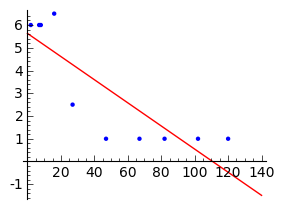
\includegraphics{bridges.png}
      \end{center}
      Apparently a better model is that
      (with only one intermediate exception) crossings in the city
      cost roughly the same as each other,
      and crossings upstate cost the same as each other.
    
\end{ans}
\begin{ans}{7}
      \begin{exparts}
        \partsitem A computer algebra system like MAPLE or MuPAD will give
          an intercept of $b=4259/1398\approx 3.239628$
          and a slope of $m=-71/2796\approx -0.025393419$
          Plugging $x=31$ into the equation yields a predicted number of
          O-ring failures of $y=2.45$ (rounded to two places).
          Plugging in $y=4$ and solving gives a temperature of
          $x=-29.94^\circ$F.
        \partsitem On the basis of this information
          \begin{equation*}
            A =
            \begin{mat}
               1 & 53 \\
               1 & 75 \\
%              1 & 57 \\
%              1 & 58 \\
%              1 & 63 \\
%              1 & 70 \\
%              1 & 70 \\
%              1 & 66 \\
%              1 & 67 \\
%              1 & 67 \\
%              1 & 67 \\
%              1 & 68 \\
%              1 & 69 \\
%              1 & 70 \\
%              1 & 70 \\
%              1 & 72 \\
%              1 & 73 \\
%              1 & 75 \\
%              1 & 76 \\
%              1 & 76 \\
%              1 & 78 \\
%              1 & 79 \\
               \vdots \\
               1 & 80 \\
               1 & 81
            \end{mat}
            \qquad
            b =
            \colvec{ 3 \\
                     2 \\
%                    1 \\
%                    1 \\
%                    1 \\
%                    1 \\
%                    1 \\
%                    0 \\
%                    0 \\
%                    0 \\
%                    0 \\
%                    0 \\
%                    0 \\
%                    0 \\
%                    0 \\
%                    0 \\
%                    0 \\
%                    0 \\
%                    0 \\
%                    0 \\
%                    0 \\
%                    0 \\
                     \vdots \\
                     0 \\
                     0}
          \end{equation*}
          MAPLE gives the intercept $b=187/40=4.675$ and the
          slope $m=-73/1200\approx -0.060833$.
          Here, plugging $x=31$ into the equation predicts
          $y=2.79$ O-ring failures (rounded to two places).
          Plugging in $y=4$~failures gives a temperature of
          $x=11^\circ$F.
     \begin{center}  \small
       \includegraphics{ch3.90}
      \end{center}
      \end{exparts}
    
\end{ans}
\begin{ans}{8}
        \begin{exparts}
          \partsitem The plot is nonlinear.
            \begin{center}  \small
              \includegraphics{ch3.91}
            \end{center}
          \partsitem Here is the plot.
           \begin{center}  \small
             \includegraphics{ch3.92}
           \end{center}
           There is perhaps a jog up between planet~$4$ and planet~$5$.
          \partsitem This plot seems even more linear.
           \begin{center}  \small
             \includegraphics{ch3.93}
           \end{center}
          \partsitem
            With this input
            \begin{equation*}
              A =
              \begin{mat}[r]
                1 & 1 \\
                1 & 2 \\
                1 & 3 \\
                1 & 4 \\
                1 & 6 \\
                1 & 7 \\
                1 & 8
              \end{mat}
              \qquad
              b = \colvec[r]{-0.40893539 \\
                          -0.1426675 \\
                           0 \\
                           0.18184359 \\
                           0.71600334 \\
                           0.97954837 \\
                           1.2833012}
            \end{equation*}
            MuPAD gives that the intercept is $b= -0.6780677466$ and
            the slope is $m=0.2372763818$.
          \partsitem Plugging $x=9$ into the equation
            $y= -0.6780677466+0.2372763818x$ from the prior item gives
            that the log of the distance is $1.4574197$, so the expected
            distance is $28.669472$.
            The actual distance is about $30.003$.
          \partsitem Plugging $x=10$ into the same equation
            gives that the log of the distance is $1.6946961$, so the expected
            distance is $49.510362$.
            The actual distance is about $39.503$.
        \end{exparts}
      
\end{ans}
\topic{Geometry of Linear Maps}
\begin{ans}{1}
      \begin{exparts}
        \partsitem  To represent $H$, recall that rotation counterclockwise by
          $\theta$~radians is represented with respect to the standard basis
          in this way.
          \begin{equation*}
            \rep{h}{\stdbasis_2,\stdbasis_2}
            =\begin{mat}
              \cos\theta  &-\sin\theta  \\
              \sin\theta  &\cos\theta
             \end{mat}
          \end{equation*}
          A clockwise angle is the negative of a counterclockwise
          one.
          \begin{equation*}
            \rep{h}{\stdbasis_2,\stdbasis_2}
            =\begin{mat}
              \cos(-\pi/4)  &-\sin(-\pi/4)  \\
              \sin(-\pi/4)  &\cos(-\pi/4)
            \end{mat}
            =\begin{mat}[r]
              \sqrt{2}/2  &\sqrt{2}/2  \\
              -\sqrt{2}/2 &\sqrt{2}/2
            \end{mat}
          \end{equation*}
          This Gauss-Jordan reduction
          \begin{equation*}
            \grstep{\rho_1+\rho_2}
            \begin{mat}[r]
              \sqrt{2}/2  &\sqrt{2}/2  \\
              0           &\sqrt{2}
            \end{mat}
            \grstep[(1/\sqrt{2})\rho_2]{(2/\sqrt{2})\rho_1}
            \begin{mat}[r]
              1  &1  \\
              0  &1
            \end{mat}
            \grstep{-\rho_2+\rho_1}
            \begin{mat}[r]
              1  &0  \\
              0  &1
            \end{mat}
          \end{equation*}
          produces the identity matrix
          so there is no need for column-swapping operations
          to end with a partial-identity.
        \partsitem In matrix multiplication the reduction is
          \begin{equation*}
            \begin{mat}[r]
              1  &-1 \\
              0  &1
            \end{mat}
            \begin{mat}[r]
              2/\sqrt{2}  &0         \\
              0           &1/\sqrt{2}
            \end{mat}
            \begin{mat}[r]
              1  &0 \\
              1  &1
            \end{mat}
            H
            =I
          \end{equation*}
          (note that composition of the Gaussian operations is
          from right to left).
        \partsitem  Taking inverses
          \begin{equation*}
            H
            =
            \underbrace{
              \begin{mat}[r]
                1  &0 \\
                -1  &1
              \end{mat}
              \begin{mat}[r]
                \sqrt{2}/2  &0         \\
                0           &\sqrt{2}
              \end{mat}
              \begin{mat}[r]
                1  &1 \\
                0  &1
              \end{mat}
             }_P
            I
          \end{equation*}
          gives the desired factorization of $H$ (here, the partial
          identity is $I$, and $Q$ is trivial, that is, it is also an identity
          matrix).
        \partsitem Reading the composition from right to left (and ignoring the
          identity matrices as trivial) gives that $H$ has the same
          effect as first performing this skew
          \begin{center}
            \includegraphics{ch3.95}
         \end{center}
         followed by a dilation that multiplies all first components by
         $\sqrt{2}/2$ (this is a ``shrink'' in that $\sqrt{2}/2\approx0.707$)
         and all second components by $\sqrt{2}$,
         followed by another skew.
          \begin{center}
            \includegraphics{ch3.96}
         \end{center}
         For instance, the effect of $H$ on the unit vector whose angle with
         the $x$-axis is $\pi/3$ is this.
          \begin{center}
            \includegraphics{ch3.97}
         \end{center}
         Verifying that the resulting vector has unit length and forms an
         angle of $-\pi/6$ with the $x$-axis is routine.
      \end{exparts}
    
\end{ans}
\begin{ans}{2}
      We will first represent the map with a matrix $H$,
      perform the row operations and, if needed, column operations
      to reduce it to a partial-identity matrix.
      We will then translate that into a factorization $H=PBQ$.
      Substituting into the general matrix
          \begin{equation*}
            \rep{r_\theta}{\stdbasis_2,\stdbasis_2}
            \begin{mat}
              \cos\theta  &-\sin\theta  \\
              \sin\theta  &\cos\theta
            \end{mat}
          \end{equation*}
          gives this representation.
          \begin{equation*}
            \rep{r_{2\pi/3}}{\stdbasis_2,\stdbasis_2}
            \begin{mat}[r]
              -1/2        &-\sqrt{3}/2  \\
              \sqrt{3}/2  &-1/2
            \end{mat}
          \end{equation*}
          Gauss's Method is routine.
          \begin{equation*}
            \grstep{\sqrt{3}\rho_1+\rho_2}
            \begin{mat}[r]
              -1/2        &-\sqrt{3}/2  \\
               0          &-2
            \end{mat}
            \grstep[(-1/2)\rho_2]{-2\rho_1}
            \begin{mat}[r]
               1          &\sqrt{3}    \\
               0          &1
            \end{mat}
            \grstep{-\sqrt{3}\rho_2+\rho_1}
            \begin{mat}[r]
               1          &0   \\
               0          &1
            \end{mat}
          \end{equation*}
          That translates to a matrix equation in this way.
          \begin{equation*}
            \begin{mat}[r]
              1  &-\sqrt{3}  \\
              0  &1
            \end{mat}
            \begin{mat}[r]
              -2  &0    \\
               0  &-1/2
            \end{mat}
            \begin{mat}[r]
               1         &0  \\
               \sqrt{3}  &1
            \end{mat}
            \begin{mat}[r]
              -1/2        &-\sqrt{3}/2  \\
              \sqrt{3}/2  &-1/2
            \end{mat}
            =I
          \end{equation*}
          Taking inverses to solve for $H$ yields this factorization.
          \begin{equation*}
            \begin{mat}[r]
              -1/2        &-\sqrt{3}/2  \\
              \sqrt{3}/2  &-1/2
            \end{mat}
            =
            \begin{mat}[r]
                1         &0  \\
               -\sqrt{3}  &1
            \end{mat}
            \begin{mat}[r]
              -1/2  &0    \\
               0    &-2
            \end{mat}
            \begin{mat}[r]
              1  &\sqrt{3}  \\
              0  &1
            \end{mat}
            I
          \end{equation*}
    
\end{ans}
\begin{ans}{3}
      This Gaussian reduction
      \begin{equation*}
        \grstep[-\rho_1+\rho_3]{-3\rho_1+\rho_2}
        \begin{mat}[r]
          1  &2  &1  \\
          0  &0  &-3 \\
          0  &0  &1
        \end{mat}
        \grstep{(1/3)\rho_2+\rho_3}
        \begin{mat}[r]
          1  &2  &1  \\
          0  &0  &-3 \\
          0  &0  &0
        \end{mat}
        \grstep{(-1/3)\rho_2}
        \begin{mat}[r]
          1  &2  &1  \\
          0  &0  &1 \\
          0  &0  &0
        \end{mat}
        \grstep{-\rho_2+\rho_1}
        \begin{mat}[r]
          1  &2  &0  \\
          0  &0  &1 \\
          0  &0  &0
        \end{mat}
      \end{equation*}
      gives the reduced echelon form of the matrix.
      Now the two column operations of taking $-2$ times the first column
      and adding it to the second, and then of swapping columns two and three
      produce this partial identity.
      \begin{equation*}
        B=\begin{mat}[r]
          1  &0  &0  \\
          0  &1  &0  \\
          0  &0  &0
        \end{mat}
      \end{equation*}
      All of that translates into matrix terms as:~where
      \begin{equation*}
        P=
        \begin{mat}[r]
          1  &-1    &0  \\
          0  &1     &0  \\
          0  &0     &1
        \end{mat}
        \begin{mat}[r]
          1  &0    &0  \\
          0  &-1/3 &0  \\
          0  &0    &1
        \end{mat}
        \begin{mat}[r]
          1  &0    &0  \\
          0  &1    &0  \\
          0  &1/3  &1
        \end{mat}
        \begin{mat}[r]
          1  &0  &0  \\
          0  &1  &0  \\
         -1  &0  &1
        \end{mat}
        \begin{mat}[r]
          1  &0  &0  \\
         -3  &1  &0  \\
          0  &0  &1
        \end{mat}
      \end{equation*}
      and
      \begin{equation*}
        Q=
        \begin{mat}[r]
          1  &-2    &0  \\
          0  &1     &0  \\
          0  &0     &1
        \end{mat}
        \begin{mat}[r]
          0  &1     &0  \\
          1  &0     &0  \\
          0  &0     &1
        \end{mat}
      \end{equation*}
      the given matrix factors as $PBQ$.
    
\end{ans}
\begin{ans}{4}
      Represent it with respect to the
      standard bases $\stdbasis_1,\stdbasis_1$, then the
      only entry in the resulting $\nbyn{1}$ matrix is the scalar $k$.
    
\end{ans}
\begin{ans}{5}
      We can show this by induction on the number of components in the
      vector.
      In the $n=1$ base case the only permutation is the trivial one,
      and the map
      \begin{equation*}
        \colvec{x_1}
        \mapsto
        \colvec{x_1}
      \end{equation*}
      is expressible as a composition of swaps\Dash as zero swaps.
      For the inductive step we assume that the map induced by
      any permutation of fewer than
      $n$ numbers can be expressed with swaps only, and we consider the map
      induced by a
      permutation $p$ of $n$ numbers.
      \begin{equation*}
        \colvec{x_1 \\ x_2 \\ \vdots \\ x_n}
        \mapsto
        \colvec{x_{p(1)} \\ x_{p(2)} \\ \vdots \\ x_{p(n)}}
      \end{equation*}
      Consider the number~$i$ such that $p(i)=n$.
      The map
      \begin{equation*}
        \colvec{x_1      \\ x_2      \\ \vdots \\ x_i      \\ \vdots \\ x_n}
        \mapsunder{\hat{p}}
        \colvec{x_{p(1)} \\ x_{p(2)} \\ \vdots \\ x_{p(n)} \\ \vdots  \\ x_{n}}
      \end{equation*}
      will, when followed by the swap of the $i$-th and $n$-th components,
      give the map~$p$.
      Now, the inductive hypothesis gives that $\hat{p}$ is achievable as
      a composition of swaps.
    
\end{ans}
\begin{ans}{6}
      \begin{exparts}
        \partsitem A line is a subset of $\Re^n$ of the form
          $\set{\vec{v}=\vec{u}+t\cdot\vec{w}\suchthat t\in\Re}$.
          The image of a point on that line is
          $h(\vec{v})=h(\vec{u}+t\cdot\vec{w})=h(\vec{u})+t\cdot h(\vec{w})$,
          and the set of such vectors, as $t$ ranges over the reals, is
          a line (albeit, degenerate if $h(\vec{w})=\zero$).
        \partsitem This is an obvious extension of the prior argument.
        \partsitem If the point~$B$ is between the points~$A$ and~$C$ then the
          line from $A$ to $C$ has $B$ in it.
          That is, there is a $t\in (0\,..\,1)$ such that
          $\vec{b}=\vec{a}+t\cdot (\vec{c}-\vec{a})$ (where $B$ is the
          endpoint of $\vec{b}$, etc.).
          Now, as in the argument of the first item, linearity shows that
          $h(\vec{b})=h(\vec{a})+t\cdot h(\vec{c}-\vec{a})$.
      \end{exparts}
    
\end{ans}
\begin{ans}{7}
      The two are inverse.
      For instance, for a fixed $x\in\Re$,
      if $f^\prime (x)=k$ (with $k\neq 0$) then
      $(f^{-1})^\prime (x)=1/k$.
      \begin{center}
        \includegraphics{ch3.98}
     \end{center}
    
\end{ans}
\topic{Magic Squares}
\begin{ans}{1}
      \begin{exparts}
        \partsitem The sum of the entries of $M$ is the sum of the sums of
          the three rows.
        \partsitem The constraints on entries of $M$ involving the center
          entry make this system.
          \begin{equation*}
            \begin{linsys}{3}
              m_{2,1}  &+  &m_{2,2}  &+  &m_{2,3}  &=  &s  \\
              m_{1,2}  &+  &m_{2,2}  &+  &m_{3,2}  &=  &s  \\
              m_{1,1}  &+  &m_{2,2}  &+  &m_{3,3}  &=  &s  \\
              m_{1,3}  &+  &m_{2,2}  &+  &m_{3,1}  &=  &s
            \end{linsys}
          \end{equation*}
          Adding those four equations counts each matrix entry once and only
          once, except that we count the center entry four times.
          Thus the left side sums to $3s+3m_{2,2}$ while the right sums to $4s$.
          So $3m_{2,2}=s$.
        \partsitem
          The second row adds to $s$ so $m_{2,1}+m_{2,2}+m_{2,3}=3m_{2,2}$,
          giving that $(1/2)\cdot(m_{2,1}+m_{2,3})=m_{2,2}$.
          The same goes for the column and the diagonals.
        \partsitem
          By the prior exercise either both $m_{2,1}$ and $m_{2,3}$ are equal
          to $m_{2,2}$ or else one is greater while one is smaller.
          Thus $m_{2,2}$ is the median of the set
          $\set{m_{2,1},m_{2,2},m_{2,3}}$.
          The same reasoning applied to the second column shows that
          Thus $m_{2,2}$ is the median of the set
          $\set{m_{1,2},m_{2,1},m_{2,2},m_{2,3},m_{3,2}}$.
          Extending to the two diagonals shows it is the median of the set
          of all entries.
      \end{exparts}
    
\end{ans}
\begin{ans}{2}
      For any $k$ we have this.
      \begin{equation*}
        \begin{amat}{4}
          1  &1  &0  &0  &s  \\
          0  &0  &1  &1  &s  \\
          1  &0  &1  &0  &s  \\
          0  &1  &0  &1  &s  \\
          1  &0  &0  &1  &s  \\
          0  &1  &1  &0  &s
        \end{amat}\;\grstep[-\rho_1+\rho_5]{-\rho_1+\rho_3}\;
        \begin{amat}{4}
          1  &1  &0  &0  &s  \\
          0  &0  &1  &1  &s  \\
          0  &-1 &1  &0  &0  \\
          0  &1  &0  &1  &s  \\
          0  &-1 &0  &1  &0  \\
          0  &1  &1  &0  &s
        \end{amat}\;\grstep{-\rho_2\leftrightarrow\rho_6}\;
        \begin{amat}{4}
          1  &1  &0  &0  &s  \\
          0  &1  &1  &0  &s  \\
          0  &-1 &1  &0  &0  \\
          0  &1  &0  &1  &s  \\
          0  &-1 &0  &1  &0  \\
          0  &0  &1  &1  &s
        \end{amat}\;\grstep[-\rho_2+\rho_4 \\ \rho_2+\rho_5]{-\rho_2+\rho_3}\;
        \begin{amat}{4}
          1  &1  &0  &0  &s  \\
          0  &1  &1  &0  &s  \\
          0  &0  &2  &0  &s  \\
          0  &1  &-1 &1  &0  \\
          0  &0  &1  &1  &s  \\
          0  &0  &1  &1  &s
        \end{amat}
      \end{equation*}
      The unique solution is $a=b=c=d=s/2$.
    
\end{ans}
\begin{ans}{3}
       By the prior exercise the only member is $Z_{\nbyn{2}}$.
    
\end{ans}
\begin{ans}{4}
      \begin{exparts}
        \partsitem
          Where $M,N\in\matspace_{\nbyn{n}}$ we have
          $\trace(cM+dN)=(cm_{1,1}+dn_{1,1})+\cdots+(cm_{n,n}+dn_{n,n})
          =(cm_{1,1}+\cdots+cm_{n,n})+(dn_{1,1}+\cdots+dn_{n,n})
          =c\cdot\trace(M)+d\cdot\trace(N)$ where
          all numbers are real, so the trace preserves linear
         combinations.
         The argument for $\trace^*$ is similar.
       \partsitem
         It preserves linear combinations: where all numbers are real,
          $\theta(cM+dN)=(\trace(cM+dN),\trace^*(cM+dN))
          =(c\cdot\trace(M)+d\cdot\trace(N), c\cdot\trace^*(M)+d\cdot\trace^*(N))
          =c\cdot\theta(M)+d\cdot\theta(N)$.
       \partsitem
         Where $\map{h_1,\ldots,h_n}{V}{W}$ are linear then so is
         $\map{g}{V}{W^n}$ given by
         $g(\vec{v})=(h_1(\vec{v}), \ldots, h_n(\vec{v}))$.
         The proof just follows the proof of the prior item.
      \end{exparts}
    
\end{ans}
\begin{ans}{5}
       \begin{exparts*}
         \partsitem
           The sum of two semimagic squares is semimagic, as is a scalar
           multiple of a semimagic square.
         \partsitem
           As with the prior item, a linear combination of two semimagic
           squares with magic number zero is also such a matrix.
       \end{exparts*}
     
\end{ans}
\begin{ans}{6}
      \begin{exparts}
        \partsitem
          Consider the matrix $C\in \mathcal{H}_n$ that has all
          entries zero except
          that the four corners are $c_{1,1}=c_{n,n}=1$ and $c_{1,n}=c_{n,1}=-1$.
           Also consider the matrix $D\in \mathcal{H}_n$ with all entries
           zero except that
           $d_{1,1}=d_{2,2}=1$ and $d_{1,2}=d_{2,1}=-1$.
           We have
           \begin{equation*}
              \theta(C)=\colvec{2 \\ -2}
              \qquad
              \theta(D)=\begin{cases}
                           \binom{2}{-1}  &\text{if $n=3$}  \\[1ex]
                           \binom{2}{0}  &\text{if $n>3$}
                        \end{cases}
           \end{equation*}
           and so the image of $\theta$ includes a basis for $\Re^2$ and
           thus $\theta$ is onto.
           With that, because for any linear map the
           dimension of the domain equals its rank plus its nullity
           we conclude that
           $\dim(\mathcal{H}_n)=2+\dim(\magicsquares_{n,0})$, as desired.
        \partsitem
           We claim that
           $\map{\phi}{\semimagicsquares_{n,0}}{\matspace_{\nbyn{(n-1)}}}$.
           is one-to-one and onto.

           To show that it is one-to-one we will show that the only member of
           $\semimagicsquares_{n,0}$ mapped to the zero matrix $Z_{\nbyn{(n-1)}}$
           is the zero matrix~$Z_{\nbyn{n}}$.
           Suppose that $M\in\semimagicsquares_{\nbyn{n}}$ and
           $\phi(M)=Z_{\nbyn{(n-1)}}$.
           On all but the final row and column $\phi$ is the identity so
           the entries in $M$ in all but the final row and column are zero:
           $m_{i,j}=0$ for $i,j\in\setinterval{1}{n-1}$.
           The first row of $M$ adds to zero and hence
           the final entry in that row $m_{1,n}$ is zero.
           Similarly the final entry in each row $i\in\setinterval{1}{n-1}$
           and column $j\in\setinterval{1}{n-1}$ is zero.
           Then, the final column adds to zero so $m_{n,n}=0$.
           Therefore $M$ is the zero matrix $Z_{\nbyn{n}}$ and the
           restriction of $\phi$
           is one-to-one.
        \partsitem
           Consider a member $\hat{M}$ of the codomain $\matspace_{\nbyn{(n-1)}}$.
           We will produce a matrix $M$ from the domain
           $\semimagicsquares_{n,0}$ that maps to it.
           The function $\phi$ is the identity on all but the final row
           and column of
           $M$ so for $i,j\in\setinterval{1}{n-1}$
           the entries are $m_{i,j}=\hat{m}_{i,j}$.
           \begin{equation*}
             M=\begin{mat}
               \hat{m}_{1,1}    &\hat{m}_{1,2}  &\ldots &\hat{m}_{1,n-1} &m_{1,n}  \\
               \vdotswithin{\hat{m}_{1,1}}
                 &\vdotswithin{\hat{m}_{1,2}}     \\
               \hat{m}_{n-1,1}  &\hat{m}_{n-1,2} &\ldots &\hat{m}_{n-1,n-1} &m_{n-1,n}  \\
               m_{n,1}         &m_{n,2}         &\ldots &m_{n,n-1}        &m_{n,n}
            \end{mat}
          \end{equation*}
          The first row of $M$ must add to zero so we take $m_{1,n}$ to be
          $-(\hat{m}_{1,1}+\cdots+\hat{m}_{1,n-1})$.
          In the same way we get the final entries
          $m_{i,n}=-(\hat{m}_{i,1}+\cdots+\hat{m}_{i,n-1})$ in all the rows but the
          bottom $i\in\setinterval{1}{n-1}$,
          and the final entries $m_{n,j}=-(\hat{m}_{1,j}+\cdots+\hat{m}_{n-1,j})$
          in all the columns but the last
          $j\in\setinterval{1}{n-1}$.
          The entry remaining is the one in the lower right~$m_{n,n}$.
          The final column adds to zero so we set it to
          $-(m_{1,n}+\cdots+m_{n-1,n})$ but we must check
          that the final row now also adds to zero.
          We have $m_{n,n}=-m_{1,n}-\cdots-m_{n-1,n}$ and expanding each of the
          $m_{i,n}$ as $-\hat{m}_{1,1}-\cdots-\hat{m}_{1,n-1}$
          gives that we have defined $m_{n,n}$ to be the sum of all the entries
          of $\hat{M}$.
          The sum of the all the entries but the last in the final row is
          $m_{1,n}+m_{2,n}+\cdots+m_{n-1,n}$ and expanding each
          $m_{n,j}=-\hat{m}_{1,j}-\cdots-\hat{m}_{n-1,j}$
          verifies that the sum of the final row is zero.
          Thus $M$ is semimagic with magic number zero and so $\phi$ is onto.
        \partsitem
           Theorem~Two.II.\ref{th:RankPlusNullEqDim} says that for any linear
           map the
           dimension of the domain equals its rank plus its nullity.
           Because $\map{\phi}{\semimagicsquares_n}{\matspace_{\nbyn{(n-1)}}}$
           is one-to-one its nullity is zero.
           Because it is onto its rank is $\dim(\matspace_{\nbyn{(n-1)}})=(n-1)^2$.
           Thus the domain of $\phi$, the subspace
           $\semimagicsquares_{n,0}$ of semimagic squares with magic number zero,
           has dimension~$(n-1)^2$.
         \partsitem
           We have that $\dim\magicsquares_n=\dim\magicsquares_{n,0}+1
           =(\dim\semimagicsquares_n-2)+1=(n-1)^2-1=n^2-n$
           when $n\geq 3$.
      \end{exparts}
    
\end{ans}
\topic{Markov Chains}
\begin{ans}{1}
      \begin{exparts}
        \partsitem With this file \texttt{coin.m}
\begin{computercode}
# Octave function for Markov coin game.  p is chance of going down.
function w = coin(p,v)
  q = 1-p;
  A=[1,p,0,0,0,0;
     0,0,p,0,0,0;
     0,q,0,p,0,0;
     0,0,q,0,p,0;
     0,0,0,q,0,0;
     0,0,0,0,q,1];
  w = A * v;
endfunction
\end{computercode}
         This Octave session produced the output given here.
\begin{computercode}
octave:1> v0=[0;0;0;1;0;0]
v0 =
  0
  0
  0
  1
  0
  0
octave:2> p=.5
p = 0.50000
octave:3> v1=coin(p,v0)
v1 =
  0.00000
  0.00000
  0.50000
  0.00000
  0.50000
  0.00000
octave:4> v2=coin(p,v1)
v2 =
  0.00000
  0.25000
  0.00000
  0.50000
  0.00000
  0.25000
\end{computercode}
This continued for too many steps to list here.
\begin{computercode}
octave:26> v24=coin(p,v23)
v24 =
  0.39600
  0.00276
  0.00000
  0.00447
  0.00000
  0.59676
\end{computercode}
        \partsitem Using these formulas
          \begin{alignat*}{2}
             p_{1}(n+1) &= 0.5\cdot p_{2}(n)
             &\qquad
             p_{2}(n+1) &= 0.5\cdot p_{1}(n)+0.5\cdot p_{3}(n)
                                                              \\
             p_{3}(n+1) &= 0.5\cdot p_{2}(n)+0.5\cdot p_{4}(n)
             &\qquad
             p_{5}(n+1) &= 0.5\cdot p_{4}(n)
          \end{alignat*}
          and these initial conditions
          \begin{equation*}
            \colvec{p_{0}(0) \\ p_{1}(0) \\ p_{2}(0) \\ p_{3}(0) \\
                        p_{4}(0) \\ p_{5}(0)}
            =
            \colvec{0 \\ 0 \\ 0 \\ 1 \\
                        0 \\ 0}
          \end{equation*}
          we will prove by induction that when $n$ is odd then
          $p_{1}(n)=p_{3}(n)=0$ and when $n$ is even then
          $p_{2}(n)=p_{4}(n)=0$.
          Note first that this is true in the $n=0$ base case by the initial
          conditions.
          For the inductive step, suppose that it is true in the
          $n=0$, $n=1$, \ldots, $n=k$~cases and consider the $n=k+1$ case.
          If $k+1$ is odd then the two
          \begin{align*}
             p_{1}(k+1) &= 0.5\cdot p_{2}(k)=0.5\cdot 0=0
                                                          \\
             p_{3}(k+1) &=0.5\cdot p_{2}(k)+0.5\cdot p_{4}(k)
                        =0.5\cdot 0+0.5\cdot 0
                        =0
          \end{align*}
          follow from the inductive hypothesis that
          $p_{2}(k)=p_{4}(k)=0$ since $k$ is even.
          The case where $k+1$ is even is similar.
        \partsitem We can use, say, $n=100$.
          This Octave session
\begin{computercode}
octave:1> B=[1,.5,0,0,0,0;
>             0,0,.5,0,0,0;
>             0,.5,0,.5,0,0;
>             0,0,.5,0,.5,0;
>             0,0,0,.5,0,0;
>             0,0,0,0,.5,1];
octave:2> B100=B**100
B100 =
  1.00000  0.80000  0.60000  0.40000  0.20000  0.00000
  0.00000  0.00000  0.00000  0.00000  0.00000  0.00000
  0.00000  0.00000  0.00000  0.00000  0.00000  0.00000
  0.00000  0.00000  0.00000  0.00000  0.00000  0.00000
  0.00000  0.00000  0.00000  0.00000  0.00000  0.00000
  0.00000  0.20000  0.40000  0.60000  0.80000  1.00000
octave:3> B100*[0;1;0;0;0;0]
octave:4> B100*[0;1;0;0;0;0]
octave:5> B100*[0;0;0;1;0;0]
octave:6> B100*[0;1;0;0;0;0]
\end{computercode}
        yields these outputs.
        \begin{equation*}
          \begin{array}{r|*{4}{c}}
            \multicolumn{1}{r}{\textit{starting with:}}
            &\text{\$1}  &\text{\$2}  &\text{\$3}  &\text{\$4} \\
             \hline
               \begin{array}{c}
                 s_{0}(100) \\
                 s_{1}(100) \\
                 s_{2}(100) \\
                 s_{3}(100) \\
                 s_{4}(100) \\
                 s_{5}(100)
               \end{array}
               &\begin{aligncolondecimal}{5}
                 0.80000 \\
                 0.00000 \\
                 0.00000 \\
                 0.00000 \\
                 0.00000 \\
                 0.20000
               \end{aligncolondecimal}
               &\begin{aligncolondecimal}{5}
                    0.60000 \\
                    0.00000 \\
                    0.00000 \\
                    0.00000 \\
                    0.00000 \\
                    0.40000
               \end{aligncolondecimal}
               &\begin{aligncolondecimal}{5}
                      0.40000 \\
                      0.00000 \\
                      0.00000 \\
                      0.00000 \\
                      0.00000 \\
                      0.60000
               \end{aligncolondecimal}
               &\begin{aligncolondecimal}{5}
                   0.20000 \\
                   0.00000 \\
                   0.00000 \\
                   0.00000 \\
                   0.00000 \\
                   0.80000
               \end{aligncolondecimal}
          \end{array}
        \end{equation*}
      \end{exparts}
    
\end{ans}
\begin{ans}{2}
      \begin{exparts}
        \partsitem From these equations
          \begin{equation*}
            \begin{linsys}{6}
              (1/6)s_{1}(n) &+ &0s_{2}(n) &+ &0s_{3}(n)
                  &+ &0s_{4}(n) &+ &0s_{5}(n)  &+ &0s_{6}(n)  &= &s_{1}(n+1) \\
              (1/6)s_{1}(n) &+ &(2/6)s_{2}(n) &+ &0s_{3}(n)
                  &+ &0s_{4}(n) &+ &0s_{5}(n)  &+ &0s_{6}(n)  &= &s_{2}(n+1) \\
              (1/6)s_{1}(n) &+ &(1/6)s_{2}(n) &+ &(3/6)s_{3}(n)
                  &+ &0s_{4}(n) &+ &0s_{5}(n)  &+ &0s_{6}(n)  &= &s_{3}(n+1) \\
              (1/6)s_{1}(n) &+ &(1/6)s_{2}(n) &+ &(1/6)s_{3}(n)
                  &+ &(4/6)s_{4}(n) &+ &0s_{5}(n)  &+ &0s_{6}(n)
                  &=  &s_{4}(n+1) \\
              (1/6)s_{1}(n) &+ &(1/6)s_{2}(n) &+ &(1/6)s_{3}(n)
                  &+ &(1/6)s_{4}(n) &+ &(5/6)s_{5}(n)  &+ &0s_{6}(n)
                  &=  &s_{5}(n+1) \\
              (1/6)s_{1}(n) &+ &(1/6)s_{2}(n) &+ &(1/6)s_{3}(n)
                  &+ &(1/6)s_{4}(n) &+ &(1/6)s_{5}(n)  &+ &(6/6)s_{6}(n)
                  &=  &s_{6}(n+1)
            \end{linsys}
          \end{equation*}
          We get this transition matrix.
          \begin{equation*}
            \begin{mat}
              1/6  &0   &0   &0   &0   &0  \\
              1/6  &2/6 &0   &0   &0   &0  \\
              1/6  &1/6 &3/6 &0   &0   &0  \\
              1/6  &1/6 &1/6 &4/6 &0   &0  \\
              1/6  &1/6 &1/6 &1/6 &5/6 &0  \\
              1/6  &1/6 &1/6 &1/6 &1/6 &6/6
            \end{mat}
          \end{equation*}
       \partsitem This is the Octave session,
         with outputs edited out and condensed into the table at the end.
\begin{computercode}
octave:1>   F=[1/6,  0,   0,   0,   0,   0;
>      1/6,  2/6, 0,   0,   0,   0;
>      1/6,  1/6, 3/6, 0,   0,   0;
>      1/6,  1/6, 1/6, 4/6, 0,   0;
>      1/6,  1/6, 1/6, 1/6, 5/6, 0;
>      1/6,  1/6, 1/6, 1/6, 1/6, 6/6];
octave:2> v0=[1;0;0;0;0;0]
octave:3> v1=F*v0
octave:4> v2=F*v1
octave:5> v3=F*v2
octave:6> v4=F*v3
octave:7> v5=F*v4
\end{computercode}
        These are the results.
        \begin{equation*}
          \begin{array}{c|*{5}{c}}
            \multicolumn{1}{c}{\ }
            &1  &2  &3  &4 &5  \\
            \hline
               \begin{aligncolondecimal}{0}
                   1 \\
                   0 \\
                   0 \\
                   0 \\
                   0 \\
                   0
               \end{aligncolondecimal}
               &\begin{aligncolondecimal}{5}
                    0.16667 \\
                    0.16667 \\
                    0.16667 \\
                    0.16667 \\
                    0.16667 \\
                    0.16667
               \end{aligncolondecimal}
               &\begin{aligncolondecimal}{6}
                   0.027778 \\
                   0.083333 \\
                   0.138889 \\
                   0.194444 \\
                   0.250000 \\
                   0.305556
               \end{aligncolondecimal}
               &\begin{aligncolondecimal}{7}
                    0.0046296 \\
                    0.0324074 \\
                    0.0879630 \\
                    0.1712963 \\
                    0.2824074 \\
                    0.4212963
               \end{aligncolondecimal}
               &\begin{aligncolondecimal}{8}
                    0.00077160 \\
                    0.01157407 \\
                    0.05015432 \\
                    0.13503086 \\
                    0.28472222 \\
                    0.51774691
               \end{aligncolondecimal}
               &\begin{aligncolondecimal}{8}
                   0.00012860 \\
                   0.00398663 \\
                   0.02713477 \\
                   0.10043724 \\
                   0.27019033 \\
                   0.59812243
               \end{aligncolondecimal}
          \end{array}
        \end{equation*}
      \end{exparts}
    
\end{ans}
\begin{ans}{3}
     \begin{exparts}
      \partsitem It does seem reasonable that, while the firm's present
        location should strongly influence where it is next time (for
        instance, whether it stays), any locations in the prior stages should
        have little influence.
        That is, while a company may move or stay because of where it is,
        it is unlikely to move or stay because of where it was.
      \partsitem This is  the Octave session, slightly edited, with the outputs
        put together in a table at the end.
\begin{lstlisting}
octave:1> M=[.787,0,0,.111,.102;
>            0,.966,.034,0,0;
>            0,.063,.937,0,0;
>            0,0,.074,.612,.314;
>            .021,.009,.005,.010,.954]
M =
  0.78700  0.00000  0.00000  0.11100  0.10200
  0.00000  0.96600  0.03400  0.00000  0.00000
  0.00000  0.06300  0.93700  0.00000  0.00000
  0.00000  0.00000  0.07400  0.61200  0.31400
  0.02100  0.00900  0.00500  0.01000  0.95400
octave:2> v0=[.025;.025;.025;.025;.900]
octave:3> v1=M*v0
octave:4> v2=M*v1
octave:5> v3=M*v2
octave:6> v4=M*v3
\end{lstlisting}
        This table summarizes.
        \begin{center}
           \begin{tabular}{c|cccc}
             $\vec{p}_0$   &$\vec{p}_1$    &$\vec{p}_2$
                    &$\vec{p}_3$   &$\vec{p}_4$    \\ \hline
             $\left(\begin{aligncolondecimal}{6}
                    0.025000 \\
                    0.025000 \\
                    0.025000 \\
                    0.025000 \\
                    0.900000
              \end{aligncolondecimal}\right)$
             &$\left(\begin{aligncolondecimal}{6}
                  0.114250 \\
                  0.025000 \\
                  0.025000 \\
                  0.299750 \\
                  0.859725
              \end{aligncolondecimal}\right)$
             &$\left(\begin{aligncolondecimal}{6}
                  0.210879 \\
                  0.025000 \\
                  0.025000 \\
                  0.455251 \\
                  0.825924
              \end{aligncolondecimal}\right)$
             &$\left(\begin{aligncolondecimal}{6}
                  0.300739 \\
                  0.025000 \\
                  0.025000 \\
                  0.539804 \\
                  0.797263
              \end{aligncolondecimal}\right)$
             &$\left(\begin{aligncolondecimal}{6}
                  0.377920 \\
                  0.025000 \\
                  0.025000 \\
                  0.582550 \\
                  0.772652
              \end{aligncolondecimal}\right)$
           \end{tabular}
       \end{center}
       \partsitem This is a continuation of the Octave session from
         the prior item.
\begin{lstlisting}
octave:7> p0=[.0000;.6522;.3478;.0000;.0000]
octave:8> p1=M*p0
octave:9> p2=M*p1
octave:10> p3=M*p2
octave:11> p4=M*p3
\end{lstlisting}
        This summarizes the output.
        \begin{center}
           \begin{tabular}{c|cccc}
             $\vec{p}_0$   &$\vec{p}_1$    &$\vec{p}_2$
                    &$\vec{p}_3$   &$\vec{p}_4$    \\ \hline
             $\left(\begin{aligncolondecimal}{5}
                  0.00000 \\
                  0.65220 \\
                  0.34780 \\
                  0.00000 \\
                  0.00000
              \end{aligncolondecimal}\right)$
             &$\left(\begin{aligncolondecimal}{5}
                  0.00000 \\
                  0.64185 \\
                  0.36698 \\
                  0.02574 \\
                  0.00761
              \end{aligncolondecimal}\right)$
             &$\left(\begin{aligncolondecimal}{7}
                  0.0036329 \\
                  0.6325047 \\
                  0.3842942 \\
                  0.0452966 \\
                  0.0151277
              \end{aligncolondecimal}\right)$
             &$\left(\begin{aligncolondecimal}{7}
                  0.0094301 \\
                  0.6240656 \\
                  0.3999315 \\
                  0.0609094 \\
                  0.0225751
              \end{aligncolondecimal}\right)$
             &$\left(\begin{aligncolondecimal}{6}
                  0.016485 \\
                  0.616445 \\
                  0.414052 \\
                  0.073960 \\
                  0.029960
              \end{aligncolondecimal}\right)$
           \end{tabular}
       \end{center}
        \partsitem This is more of the same Octave session.
\begin{lstlisting}
octave:12> M50=M**50
M50 =
  0.03992  0.33666  0.20318  0.02198  0.37332
  0.00000  0.65162  0.34838  0.00000  0.00000
  0.00000  0.64553  0.35447  0.00000  0.00000
  0.03384  0.38235  0.22511  0.01864  0.31652
  0.04003  0.33316  0.20029  0.02204  0.37437
octave:13> p50=M50*p0
p50 =
  0.29024
  0.54615
  0.54430
  0.32766
  0.28695
octave:14> p51=M*p50
p51 =
  0.29406
  0.54609
  0.54442
  0.33091
  0.29076
\end{lstlisting}
        This is close to a steady state.
      \end{exparts}
    
\end{ans}
\begin{ans}{4}
      \begin{exparts}
        \partsitem This is the relevant system of equations.
          \begin{equation*}
            \begin{linsys}{5}
              (1-2p)\cdot s_{U}(n)  &+ &p\cdot t_{A}(n)  &+  &p\cdot t_{B}(n)
                &  &  &  &
                &=  &s_{U}(n+1)            \\
              p\cdot s_{U}(n)  &+  &(1-2p)\cdot t_{A}(n)  &  &  &  &  &  &
                &=  &t_{A}(n+1)            \\
              p\cdot s_{U}(n)  &  &  &+  &(1-2p)\cdot t_{B}(n)  &  &  &  &
                &=  &t_{B}(n+1)            \\
                &  &p\cdot t_{A}(n)  &  &  &+  &s_{A}(n)  &  &
                &=  &s_{A}(n+1)            \\
                &  &  &   &p\cdot t_{B}(n)  &  &  &+  &s_{B}(n)
                &=  &s_{B}(n+1)
            \end{linsys}
          \end{equation*}
          Thus we have this.
          \begin{equation*}
            \begin{pmatrix}
              1-2p &p     &p    &0  &0  \\
              p    &1-2p  &0    &0  &0  \\
              p    &0     &1-2p &0  &0  \\
              0    &p     &0    &1  &0  \\
              0    &0     &p    &0  &1
            \end{pmatrix}
            \colvec{s_{U}(n) \\ t_{A}(n) \\ t_{B}(n) \\ s_{A}(n) \\ s_{B}(n)}
            =
            \colvec{s_{U}(n+1) \\ t_{A}(n+1) \\ t_{B}(n+1)
                                     \\ s_{A}(n+1) \\ s_{B}(n+1)}
          \end{equation*}
        \partsitem This is the Octave code, with the output removed.
\begin{lstlisting}
octave:1> T=[.5,.25,.25,0,0;
>            .25,.5,0,0,0;
>            .25,0,.5,0,0;
>            0,.25,0,1,0;
>            0,0,.25,0,1]
T =
  0.50000  0.25000  0.25000  0.00000  0.00000
  0.25000  0.50000  0.00000  0.00000  0.00000
  0.25000  0.00000  0.50000  0.00000  0.00000
  0.00000  0.25000  0.00000  1.00000  0.00000
  0.00000  0.00000  0.25000  0.00000  1.00000
octave:2> p0=[1;0;0;0;0]
octave:3> p1=T*p0
octave:4> p2=T*p1
octave:5> p3=T*p2
octave:6> p4=T*p3
octave:7> p5=T*p4
\end{lstlisting}
        Here is the output.
        The probability of ending at $s_A$ is about $0.23$.
        \begin{equation*}
          \begin{array}{cc|ccccc}
            &\vec{p}_0 &\vec{p}_1 &\vec{p}_2 &\vec{p}_3
                &\vec{p}_4 &\vec{p}_5 \\
            \hline
            \begin{array}{c}
              s_U \\
              t_A \\
              t_B \\
              s_A \\
              s_B
            \end{array}
            &\begin{array}{c}
               1 \\
               0 \\
               0 \\
               0 \\
               0
            \end{array}
            &\begin{array}{c}
              0.50000 \\
              0.25000 \\
              0.25000 \\
              0.00000 \\
              0.00000
            \end{array}
            &\begin{array}{c}
              0.375000 \\
              0.250000 \\
              0.250000 \\
              0.062500 \\
              0.062500
            \end{array}
            &\begin{array}{c}
              0.31250 \\
              0.21875 \\
              0.21875 \\
              0.12500 \\
              0.12500
            \end{array}
            &\begin{array}{c}
              0.26562 \\
              0.18750 \\
              0.18750 \\
              0.17969 \\
              0.17969
            \end{array}
            &\begin{array}{c}
              0.22656 \\
              0.16016 \\
              0.16016 \\
              0.22656 \\
              0.22656
            \end{array}
          \end{array}
        \end{equation*}
       \partsitem With this file as \texttt{learn.m}
\begin{lstlisting}
# Octave script file for learning model.
function w = learn(p)
   T = [1-2*p,p,    p,    0, 0;
        p,    1-2*p,0,    0, 0;
        p,    0,    1-2*p,0, 0;
        0,    p,    0,    1, 0;
        0,    0,    p,    0, 1];
  T5 = T**5;
  p5 = T5*[1;0;0;0;0];
  w = p5(4);
endfunction
\end{lstlisting}
        issuing the command \texttt{octave:1> learn(.20)} yields
        \texttt{ans = 0.17664}.
       \partsitem This Octave session
\begin{lstlisting}
octave:1> x=(.01:.01:.50)';
octave:2> y=(.01:.01:.50)';
octave:3> for i=.01:.01:.50
>           y(100*i)=learn(i);
>         endfor
octave:4> z=[x, y];
octave:5> gplot z
\end{lstlisting}
        yields this plot.
        There is no threshold value \Dash  no probability above which the
        curve rises sharply.
        \begin{center}
          \includegraphics{learn5.eps}
        \end{center}
      \end{exparts}
    
\end{ans}
\begin{ans}{5}
       \begin{exparts}
         \partsitem From these equations
           \begin{equation*}
             \begin{linsys}{2}
               0.90\cdot p_{T}(n)  &+  &0.01\cdot p_{C}(n) &= &p_{T}(n+1)   \\
               0.10\cdot p_{T}(n)  &+  &0.99\cdot p_{C}(n) &= &p_{C}(n+1)
             \end{linsys}
           \end{equation*}
           we get this matrix.
           \begin{equation*}
             \begin{pmatrix}
               0.90  &0.01  \\
               0.10  &0.99
             \end{pmatrix}
             \colvec{p_{T}(n) \\ p_{C}(n)}
             =
             \colvec{p_{T}(n+1) \\ p_{C}(n+1)}
           \end{equation*}
         \partsitem This is the result from Octave.
           \begin{center}
             \begin{tabular}{c|ccccc}
               $n=0$ &1  &2  &3  &4  &5  \\
               \hline
               $\begin{array}{c}  0.30000 \\ 0.70000 \end{array}$
               &$\begin{array}{c} 0.27700 \\ 0.72300 \end{array}$
               &$\begin{array}{c}  0.25653 \\ 0.74347 \end{array}$
               &$\begin{array}{c}  0.23831 \\ 0.76169 \end{array}$
               &$\begin{array}{c}  0.22210 \\ 0.77790 \end{array}$
               &$\begin{array}{c}  0.20767 \\ 0.79233 \end{array}$
             \end{tabular}                                     \\[1ex]
             \begin{tabular}{|ccccc}
               6  &7  &8  &9 &10 \\
               \hline
               $\begin{array}{c}  0.19482 \\ 0.80518 \end{array}$
               &$\begin{array}{c}  0.18339 \\ 0.81661 \end{array}$
               &$\begin{array}{c}  0.17322 \\ 0.82678 \end{array}$
               &$\begin{array}{c}  0.16417 \\ 0.83583 \end{array}$
               &$\begin{array}{c}  0.15611 \\ 0.84389 \end{array}$
             \end{tabular}
           \end{center}
         \partsitem This is the $s_T=0.2$ result.
           \begin{center}
             \begin{tabular}{c|ccccc}
               $n=0$ &1  &2  &3  &4  &5  \\
               \hline
               $\begin{array}{c}  0.20000 \\ 0.80000 \end{array}$
               &$\begin{array}{c}   0.18800 \\ 0.81200 \end{array}$
               &$\begin{array}{c}   0.17732 \\ 0.82268 \end{array}$
               &$\begin{array}{c}   0.16781 \\ 0.83219 \end{array}$
               &$\begin{array}{c}   0.15936 \\ 0.84064 \end{array}$
               &$\begin{array}{c}   0.15183 \\ 0.84817 \end{array}$
             \end{tabular}                                         \\[1ex]
             \begin{tabular}{|ccccc}
               6  &7  &8  &9 &10 \\
               \hline
               $\begin{array}{c}  0.14513 \\ 0.85487  \end{array}$
               &$\begin{array}{c}  0.13916 \\ 0.86084  \end{array}$
               &$\begin{array}{c}  0.13385 \\ 0.86615  \end{array}$
               &$\begin{array}{c}  0.12913 \\ 0.87087  \end{array}$
               &$\begin{array}{c}  0.12493 \\ 0.87507  \end{array}$
             \end{tabular}
           \end{center}
          \partsitem Although the probability vectors start $0.1$ apart,
            they end only $0.032$ apart.
            So they are alike.
       \end{exparts}
     
\end{ans}
\begin{ans}{6}
     These are the $p=.55$ vectors,
     \begin{center}\small
       \begin{tabular}{@{}rc|ccccccc@{}}
         &$n=0$  &$n=1$  &$n=2$  &$n=3$  &$n=4$  &$n=5$  &$n=6$  &$n=7$  \\
        \hline
        \begin{tabular}{@{}c@{}}
           0-0 \\
           1-0 \\
           0-1 \\
           2-0 \\
           1-1 \\
           0-2 \\
           3-0 \\
           2-1 \\
           1-2 \\
           0-3 \\
           4-0 \\
           3-1 \\
           2-2 \\
           1-3 \\
           0-4 \\
           4-1 \\
           3-2 \\
           2-3 \\
           1-4 \\
           4-2 \\
           3-3 \\
           2-4 \\
           4-3 \\
           3-4
         \end{tabular}
          &$\begin{aligncolondecimal}{0}
             1 \\
             0 \\
             0 \\
             0 \\
             0 \\
             0 \\
             0 \\
             0 \\
             0 \\
             0 \\
             0 \\
             0 \\
             0 \\
             0 \\
             0 \\
             0 \\
             0 \\
             0 \\
             0 \\
             0 \\
             0 \\
             0 \\
             0 \\
             0
           \end{aligncolondecimal}$
         &$\begin{aligncolondecimal}{5}
           0 \\
           0.55000 \\
           0.45000 \\
           0 \\
           0 \\
           0 \\
           0 \\
           0 \\
           0 \\
           0 \\
           0 \\
           0 \\
           0 \\
           0 \\
           0 \\
           0 \\
           0 \\
           0 \\
           0 \\
           0 \\
           0 \\
           0 \\
           0 \\
           0
         \end{aligncolondecimal}$
         &$\begin{aligncolondecimal}{5}
           0 \\
           0 \\
           0 \\
           0.30250 \\
           0.49500 \\
           0.20250 \\
           0 \\
           0 \\
           0 \\
           0 \\
           0 \\
           0 \\
           0 \\
           0 \\
           0 \\
           0 \\
           0 \\
           0 \\
           0 \\
           0 \\
           0 \\
           0 \\
           0 \\
           0
         \end{aligncolondecimal}$
         &$\begin{aligncolondecimal}{5}
           0 \\
           0 \\
           0 \\
           0 \\
           0 \\
           0 \\
           0.16638 \\
           0.40837 \\
           0.33412 \\
           0.09112 \\
           0 \\
           0 \\
           0 \\
           0 \\
           0 \\
           0 \\
           0 \\
           0 \\
           0 \\
           0 \\
           0 \\
           0 \\
           0 \\
           0
         \end{aligncolondecimal}$
         &$\begin{aligncolondecimal}{5}
           0 \\
           0 \\
           0 \\
           0 \\
           0 \\
           0 \\
           0 \\
           0 \\
           0 \\
           0 \\
           0.09151 \\
           0.29948 \\
           0.36754 \\
           0.20047 \\
           0.04101 \\
           0 \\
           0 \\
           0 \\
           0 \\
           0 \\
           0 \\
           0 \\
           0 \\
           0
         \end{aligncolondecimal}$
         &$\begin{aligncolondecimal}{5}
          0 \\
          0 \\
          0 \\
          0 \\
          0 \\
          0 \\
          0 \\
          0 \\
          0 \\
          0 \\
          0.09151 \\
          0 \\
          0 \\
          0 \\
          0.04101 \\
          0.16471 \\
          0.33691 \\
          0.27565 \\
          0.09021 \\
          0 \\
          0 \\
          0 \\
          0 \\
          0
         \end{aligncolondecimal}$
         &$\begin{aligncolondecimal}{5}
          0 \\
          0 \\
          0 \\
          0 \\
          0 \\
          0 \\
          0 \\
          0 \\
          0 \\
          0 \\
          0.09151 \\
          0 \\
          0 \\
          0 \\
          0.04101 \\
          0.16471 \\
          0 \\
          0 \\
          0.09021 \\
          0.18530 \\
          0.30322 \\
          0.12404 \\
          0 \\
          0
         \end{aligncolondecimal}$
         &$\begin{aligncolondecimal}{5}
          0 \\
          0 \\
          0 \\
          0 \\
          0 \\
          0 \\
          0 \\
          0 \\
          0 \\
          0 \\
          0.09151 \\
          0 \\
          0 \\
          0 \\
          0.04101 \\
          0.16471 \\
          0 \\
          0 \\
          0.09021 \\
          0.18530 \\
          0 \\
          0.12404 \\
          0.16677 \\
          0.13645
         \end{aligncolondecimal}$
       \end{tabular}
       \end{center}
       and these are the $p=.60$ vectors.
       \begin{center}\small
       \begin{tabular}{@{}rc|ccccccc@{}}
         &$n=0$  &$n=1$  &$n=2$  &$n=3$  &$n=4$  &$n=5$  &$n=6$  &$n=7$  \\
        \hline
        \begin{tabular}{@{}c@{}}
           0-0 \\
           1-0 \\
           0-1 \\
           2-0 \\
           1-1 \\
           0-2 \\
           3-0 \\
           2-1 \\
           1-2 \\
           0-3 \\
           4-0 \\
           3-1 \\
           2-2 \\
           1-3 \\
           0-4 \\
           4-1 \\
           3-2 \\
           2-3 \\
           1-4 \\
           4-2 \\
           3-3 \\
           2-4 \\
           4-3 \\
           3-4
         \end{tabular}
          &$\begin{aligncolondecimal}{0}
             1 \\
             0 \\
             0 \\
             0 \\
             0 \\
             0 \\
             0 \\
             0 \\
             0 \\
             0 \\
             0 \\
             0 \\
             0 \\
             0 \\
             0 \\
             0 \\
             0 \\
             0 \\
             0 \\
             0 \\
             0 \\
             0 \\
             0 \\
             0
           \end{aligncolondecimal}$
         &$\begin{aligncolondecimal}{5}
          0 \\
          0.60000 \\
          0.40000 \\
          0 \\
          0 \\
          0 \\
          0 \\
          0 \\
          0 \\
          0 \\
          0 \\
          0 \\
          0 \\
          0 \\
          0 \\
          0 \\
          0 \\
          0 \\
          0 \\
          0 \\
          0 \\
          0 \\
          0 \\
          0
         \end{aligncolondecimal}$
         &$\begin{aligncolondecimal}{5}
            0 \\
            0 \\
            0 \\
            0.36000 \\
            0.48000 \\
            0.16000 \\
            0 \\
            0 \\
            0 \\
            0 \\
            0 \\
            0 \\
            0 \\
            0 \\
            0 \\
            0 \\
            0 \\
            0 \\
            0 \\
            0 \\
            0 \\
            0 \\
            0 \\
            0
         \end{aligncolondecimal}$
         &$\begin{aligncolondecimal}{5}
            0 \\
            0 \\
            0 \\
            0 \\
            0 \\
            0 \\
            0.21600 \\
            0.43200 \\
            0.28800 \\
            0.06400 \\
            0 \\
            0 \\
            0 \\
            0 \\
            0 \\
            0 \\
            0 \\
            0 \\
            0 \\
            0 \\
            0 \\
            0 \\
            0 \\
            0
         \end{aligncolondecimal}$
         &$\begin{aligncolondecimal}{5}
            0 \\
            0 \\
            0 \\
            0 \\
            0 \\
            0 \\
            0 \\
            0 \\
            0 \\
            0 \\
            0.12960 \\
            0.34560 \\
            0.34560 \\
            0.15360 \\
            0.02560 \\
            0 \\
            0 \\
            0 \\
            0 \\
            0 \\
            0 \\
            0 \\
            0 \\
            0
         \end{aligncolondecimal}$
         &$\begin{aligncolondecimal}{5}
             0 \\
             0 \\
             0 \\
             0 \\
             0 \\
             0 \\
             0 \\
             0 \\
             0 \\
             0 \\
             0.12960 \\
             0 \\
             0 \\
             0 \\
             0.02560 \\
             0.20736 \\
             0.34560 \\
             0.23040 \\
             0.06144 \\
             0 \\
             0 \\
             0 \\
             0 \\
             0
         \end{aligncolondecimal}$
         &$\begin{aligncolondecimal}{5}
            0 \\
            0 \\
            0 \\
            0 \\
            0 \\
            0 \\
            0 \\
            0 \\
            0 \\
            0 \\
            0.12960 \\
            0 \\
            0 \\
            0 \\
            0.02560 \\
            0.20736 \\
            0 \\
            0 \\
            0.06144 \\
            0.20736 \\
            0.27648 \\
            0.09216 \\
            0 \\
            0
         \end{aligncolondecimal}$
         &$\begin{aligncolondecimal}{5}
            0 \\
            0 \\
            0 \\
            0 \\
            0 \\
            0 \\
            0 \\
            0 \\
            0 \\
            0 \\
            0.12960 \\
            0 \\
            0 \\
            0 \\
            0.02560 \\
            0.20736 \\
            0 \\
            0 \\
            0.06144 \\
            0.20736 \\
            0 \\
            0.09216 \\
            0.16589 \\
            0.11059
         \end{aligncolondecimal}$
       \end{tabular}
     \end{center}
     \begin{exparts}
      \partsitem We can adapt the script from the end of this Topic.
\begin{lstlisting}
# Octave script file to compute chance of World Series outcomes.
function w = markov(p,v)
  q = 1-p;
  A=[0,0,0,0,0,0, 0,0,0,0,0,0, 0,0,0,0,0,0, 0,0,0,0,0,0;  # 0-0
     p,0,0,0,0,0, 0,0,0,0,0,0, 0,0,0,0,0,0, 0,0,0,0,0,0;  # 1-0
     q,0,0,0,0,0, 0,0,0,0,0,0, 0,0,0,0,0,0, 0,0,0,0,0,0;  # 0-1_
     0,p,0,0,0,0, 0,0,0,0,0,0, 0,0,0,0,0,0, 0,0,0,0,0,0;  # 2-0
     0,q,p,0,0,0, 0,0,0,0,0,0, 0,0,0,0,0,0, 0,0,0,0,0,0;  # 1-1
     0,0,q,0,0,0, 0,0,0,0,0,0, 0,0,0,0,0,0, 0,0,0,0,0,0;  # 0-2__
     0,0,0,p,0,0, 0,0,0,0,0,0, 0,0,0,0,0,0, 0,0,0,0,0,0;  # 3-0
     0,0,0,q,p,0, 0,0,0,0,0,0, 0,0,0,0,0,0, 0,0,0,0,0,0;  # 2-1
     0,0,0,0,q,p, 0,0,0,0,0,0, 0,0,0,0,0,0, 0,0,0,0,0,0;  # 1-2_
     0,0,0,0,0,q, 0,0,0,0,0,0, 0,0,0,0,0,0, 0,0,0,0,0,0;  # 0-3
     0,0,0,0,0,0, p,0,0,0,1,0, 0,0,0,0,0,0, 0,0,0,0,0,0;  # 4-0
     0,0,0,0,0,0, q,p,0,0,0,0, 0,0,0,0,0,0, 0,0,0,0,0,0;  # 3-1__
     0,0,0,0,0,0, 0,q,p,0,0,0, 0,0,0,0,0,0, 0,0,0,0,0,0;  # 2-2
     0,0,0,0,0,0, 0,0,q,p,0,0, 0,0,0,0,0,0, 0,0,0,0,0,0;  # 1-3
     0,0,0,0,0,0, 0,0,0,q,0,0, 0,0,1,0,0,0, 0,0,0,0,0,0;  # 0-4_
     0,0,0,0,0,0, 0,0,0,0,0,p, 0,0,0,1,0,0, 0,0,0,0,0,0;  # 4-1
     0,0,0,0,0,0, 0,0,0,0,0,q, p,0,0,0,0,0, 0,0,0,0,0,0;  # 3-2
     0,0,0,0,0,0, 0,0,0,0,0,0, q,p,0,0,0,0, 0,0,0,0,0,0;  # 2-3__
     0,0,0,0,0,0, 0,0,0,0,0,0, 0,q,0,0,0,0, 1,0,0,0,0,0;  # 1-4
     0,0,0,0,0,0, 0,0,0,0,0,0, 0,0,0,0,p,0, 0,1,0,0,0,0;  # 4-2
     0,0,0,0,0,0, 0,0,0,0,0,0, 0,0,0,0,q,p, 0,0,0,0,0,0;  # 3-3_
     0,0,0,0,0,0, 0,0,0,0,0,0, 0,0,0,0,0,q, 0,0,0,1,0,0;  # 2-4
     0,0,0,0,0,0, 0,0,0,0,0,0, 0,0,0,0,0,0, 0,0,p,0,1,0;  # 4-3
     0,0,0,0,0,0, 0,0,0,0,0,0, 0,0,0,0,0,0, 0,0,q,0,0,1]; # 3-4
  v7 = (A**7) * v;
  w = v7(11)+v7(16)+v7(20)+v7(23)
endfunction
\end{lstlisting}
       Using this script, we get that when the American League has a
       $p=0.55$ probability of winning each game then their probability
       of winning the first-to-win-four series is $0.60829$.
       When their probability of winning any one game is $p=0.6$
       then their probability of winning the series is
       $0.71021$.
      \partsitem This Octave session
\begin{lstlisting}
octave:1> v0=[1;0;0;0;0;0;0;0;0;0;0;0;0;0;0;0;0;0;0;0;0;0;0;0];
octave:2> x=(.01:.01:.99)';
octave:3> y=(.01:.01:.99)';
octave:4> for i=.01:.01:.99
>          y(100*i)=markov(i,v0);
>         endfor
octave:5> z=[x, y];
octave:6> gplot z
\end{lstlisting}
       yields this graph.
       By eye we judge that if $p>0.7$ then the team is close to assured
       of the series.
       \begin{center}
         \includegraphics{ws.eps}
       \end{center}
     \end{exparts}
    
\end{ans}
\begin{ans}{7}
      \begin{exparts}
        \partsitem They must satisfy this condition because the total
          probability of a state transition (including back to the
          same state) is $100\%$.
        \partsitem See the answer to the third item.
        \partsitem We will
          do the $\nbyn{2}$ case; bigger-sized cases are just notational
          problems.
          This product
          \begin{equation*}
            \begin{pmatrix}
              a_{1,1}  &a_{1,2}  \\
              a_{2,1}  &a_{2,2}
            \end{pmatrix}
            \begin{pmatrix}
              b_{1,1}  &b_{1,2}  \\
              b_{2,1}  &b_{2,2}
            \end{pmatrix}
            =\begin{pmatrix}
              a_{1,1}b_{1,1}+a_{1,2}b_{2,1}  &a_{1,1}b_{1,2}+a_{1,2}b_{2,2} \\
              a_{2,1}b_{1,1}+a_{2,2}b_{2,1}  &a_{2,1}b_{1,2}+a_{2,2}b_{2,2} \\
            \end{pmatrix}
           \end{equation*}
            has these two column sums
            \begin{equation*}
              (a_{1,1}b_{1,1}+a_{1,2}b_{2,1})
              +(a_{2,1}b_{1,1}+a_{2,2}b_{2,1})
              =(a_{1,1}+a_{2,1})\cdot b_{1,1}
                +(a_{1,2}+a_{2,2})\cdot b_{2,1}
              =1\cdot b_{1,1}+1\cdot b_{2,1}
              =1
            \end{equation*}
            and
            \begin{equation*}
              (a_{1,1}b_{1,2}+a_{1,2}b_{2,2})
              +(a_{2,1}b_{1,2}+a_{2,2}b_{2,2})
              =(a_{1,1}+a_{2,1})\cdot b_{1,2}
                +(a_{1,2}+a_{2,2})\cdot b_{2,2}
              =1\cdot b_{1,2}+1\cdot b_{2,2}
              =1
            \end{equation*}
            as required.
      \end{exparts}
    
\end{ans}
\topic{Orthonormal Matrices}
\begin{ans}{1}
      \begin{exparts}
        \partsitem Yes.
        \partsitem No, the columns do not have length one.
        \partsitem Yes.
      \end{exparts}
    
\end{ans}
\begin{ans}{2}
      Some of these are nonlinear,
      because they involve a nontrivial translation.
      \begin{exparts}
        \partsitem
          $\colvec{x \\ y}
           \mapsto
           \begin{mat}
             x\cdot\cos(\pi/6)-y\cdot\sin(\pi/6) \\
             x\cdot\sin(\pi/6)+y\cdot\cos(\pi/6)
           \end{mat}
           +\colvec[r]{0 \\ 1}
           =\begin{mat}
             x\cdot(\sqrt{3}/2)-y\cdot(1/2)+0 \\
             x\cdot(1/2)+y\cdot\cos(\sqrt{3}/2)+1
           \end{mat}$
        \partsitem The line $y=2x$ makes an angle of $\arctan(2/1)$
          with the $x$-axis.
          Thus $\sin\theta=2/\sqrt{5}$ and $\cos\theta=1/\sqrt{5}$.
          \begin{equation*}
          \colvec{x \\ y}
           \mapsto
           \begin{mat}
             x\cdot(1/\sqrt{5})-y\cdot(2/\sqrt{5}) \\
             x\cdot(2/\sqrt{5})+y\cdot(1/\sqrt{5})
           \end{mat}
           \end{equation*}
        \partsitem
           $\colvec{x \\ y}
           \mapsto
           \begin{mat}
             x\cdot(1/\sqrt{5})-y\cdot(-2/\sqrt{5}) \\
             x\cdot(-2/\sqrt{5})+y\cdot(1/\sqrt{5})
           \end{mat}
           +\colvec[r]{1 \\ 1}
           =\begin{mat}
             x/\sqrt{5}+2y/\sqrt{5}+1 \\
             -2x/\sqrt{5}+y/\sqrt{5}+1
           \end{mat}$
      \end{exparts}
    
\end{ans}
\begin{ans}{3}
       \begin{exparts}
         \partsitem Let $f$ be distance-preserving and consider $f^{-1}$.
           Any two points in the codomain can be written as $f(P_1)$ and
           $f(P_2)$.
           Because $f$ is distance-preserving, the distance from $f(P_1)$
           to $f(P_2)$ equals the distance from $P_1$ to $P_2$.
           But this is exactly what is required for $f^{-1}$ to be
           distance-preserving.
         \partsitem Any plane figure $F$ is congruent to itself via the
           identity map $\map{\identity}{\Re^2}{\Re^2}$, which is obviously
           distance-preserving.
           If $F_1$ is congruent to $F_2$ (via some $f$) then
           $F_2$ is congruent to $F_1$ via $f^{-1}$, which is
           distance-preserving by the prior item.
           Finally, if $F_1$ is congruent to $F_2$ (via some $f$) and
           $F_2$ is congruent to $F_3$ (via some $g$) then $F_1$ is
           congruent to $F_3$ via $\composed{g}{f}$, which is easily checked
           to be distance-preserving.
       \end{exparts}
     
\end{ans}
\begin{ans}{4}
       The first two components of each are $ax+cy+e$ and $bx+dy+f$.
     
\end{ans}
\begin{ans}{5}
      \begin{exparts}
        \partsitem The Pythagorean Theorem gives that
          three points are
          colinear if and only if
          (for some ordering of them into $P_1$, $P_2$, and $P_3$),
          $\dist(P_1,P_2)+\dist(P_2,P_3)=\dist(P_1,P_3)$.
          Of course, where $f$ is distance-preserving, this holds
          if and only if
          $\dist(f(P_1),f(P_2))+\dist(f(P_2),f(P_3))=\dist(f(P_1),f(P_3))$,
          which, again by Pythagoras, is true if and only if
          $f(P_1)$, $f(P_2)$, and $f(P_3)$ are colinear.

          The argument for betweeness is similar (above, $P_2$ is
          between $P_1$ and $P_3$).

          If the figure $F$ is a triangle then it is the union of three
          line segments $P_1P_2$, $P_2P_3$, and $P_1P_3$.
          The prior two paragraphs together show that the property of
          being a line segment is invariant.
          So $f(F)$ is the union of three line segments, and so is a
          triangle.

          A circle $C$ centered at $P$ and of radius $r$ is the set of
          all points $Q$ such that $\dist(P,Q)=r$.
          Applying the distance-preserving map $f$ gives that the image
          $f(C)$ is the set of all $f(Q)$ subject to the condition that
          $\dist(P,Q)=r$.
          Since $\dist(P,Q)=\dist(f(P),f(Q))$, the set $f(C)$ is also
          a circle, with center $f(P)$ and radius $r$.
        \partsitem Here are two that are easy to verify: (i)~the
          property of being a right triangle, and (ii)~the property of
          two lines being parallel.
        \partsitem One that was mentioned in the section is the `sense' of
          a figure.
          A triangle whose vertices read clockwise as $P_1$, $P_2$, $P_3$
          may, under a distance-preserving map, be sent to a triangle
          read $P_1$, $P_2$, $P_3$ counterclockwise.
      \end{exparts}
    
\end{ans}
\chapter{Chapter Four: Determinants}
\section{Def{}inition}
\subsection{Four.I.1: Exploration}
\begin{ans}{Four.I.1.1}
       \begin{exparts*}
         \partsitem \( 4 \)
         \partsitem \( 3 \)
         \partsitem \( -12 \)
       \end{exparts*}
     
\end{ans}
\begin{ans}{Four.I.1.2}
      \begin{exparts*}
        \partsitem \( 6 \)
        \partsitem \( 21 \)
        \partsitem \( 27 \)
      \end{exparts*}
    
\end{ans}
\begin{ans}{Four.I.1.3}
      For the first, apply the formula in this section, note that any
      term with a \( d \), \( g \), or \( h \) is zero, and simplify.
      Lower-triangular matrices work the same way.
    
\end{ans}
\begin{ans}{Four.I.1.4}
       \begin{exparts}
         \partsitem Nonsingular, the determinant is \( -1 \).
         \partsitem Nonsingular, the determinant is \( -1 \).
         \partsitem Singular, the determinant is \( 0 \).
       \end{exparts}
     
\end{ans}
\begin{ans}{Four.I.1.5}
      \begin{exparts}
         \partsitem Nonsingular, the determinant is \( 3 \).
         \partsitem Singular, the determinant is \( 0 \).
         \partsitem Singular, the determinant is \( 0 \).
       \end{exparts}
     
\end{ans}
\begin{ans}{Four.I.1.6}
       \begin{exparts}
         \partsitem \( \det(B)=\det(A) \) via \( -2\rho_1+\rho_2 \)
         \partsitem \( \det(B)=-\det(A) \) via
             \( \rho_2\leftrightarrow\rho_3 \)
         \partsitem \( \det(B)=(1/2)\cdot \det(A) \) via \( (1/2)\rho_2 \)
       \end{exparts}
     
\end{ans}
\begin{ans}{Four.I.1.7}
       Using the formula for the determinant of a $\nbyn{3}$ matrix
       we expand the left side
       \begin{equation*}
         1\cdot b\cdot c^2+1\cdot c\cdot a^2+1\cdot a\cdot b^2
          -b^2\cdot c\cdot 1 -c^2\cdot a\cdot 1-a^2\cdot b\cdot 1
       \end{equation*}
       and by distributing we expand the right side.
       \begin{equation*}
         (bc-ba-ac+a^2)\cdot(c-b)
         =c^2b-b^2c-bac+b^2a-ac^2+acb+a^2c-a^2b
       \end{equation*}
       Now we can just check that the two are equal.
       (\textit{Remark}.
       This is the \( \nbyn{3} \) case of
       \definend{Vandermonde's determinant}\index{Vandermonde!determinant}%
       \index{determinant!Vandermonde} which arises in applications).
     
\end{ans}
\begin{ans}{Four.I.1.8}
         This equation
         \begin{equation*}
           0=
           \det(
             \begin{mat}
                12-x  &4  \\
                8    &8-x
             \end{mat}
           )
           =64-20x+x^2
           =(x-16)(x-4)
       \end{equation*}
       has roots \( x=16 \) and \( x=4 \).
     
\end{ans}
\begin{ans}{Four.I.1.9}
      We first reduce the matrix to echelon form.
      To begin, assume that \( a\neq 0 \) and that \( ae-bd\neq 0 \).
      \begin{eqnarray*}
        \grstep{(1/a)\rho_1}\;
        \begin{mat}
           1   &b/a   &c/a   \\
           d   &e     &f     \\
           g   &h     &i
         \end{mat}
        &\grstep[-g\rho_1+\rho_3]{-d\rho_1+\rho_2}
        &\begin{mat}
           1   &b/a           &c/a           \\
           0   &(ae-bd)/a     &(af-cd)/a     \\
           0   &(ah-bg)/a     &(ai-cg)/a
         \end{mat}                                            \\
        &\grstep{(a/(ae-bd))\rho_2}
        &\begin{mat}
           1   &b/a           &c/a             \\
           0   &1             &(af-cd)/(ae-bd) \\
           0   &(ah-bg)/a     &(ai-cg)/a
         \end{mat}
      \end{eqnarray*}
      This step finishes the calculation.
      \begin{equation*}
        \grstep{((ah-bg)/a)\rho_2+\rho_3}
        \begin{mat}
           1   &b/a    &c/a             \\
           0   &1      &(af-cd)/(ae-bd)      \\
           0   &0      &(aei+bgf+cdh-hfa-idb-gec)/(ae-bd)
         \end{mat}
      \end{equation*}
      Now assuming that $a\neq 0$ and \( ae-bd\neq 0 \),
      the original matrix is nonsingular
      if and only if the \( 3,3 \) entry above is nonzero.
      That is, under the assumptions, the original matrix is
      nonsingular if and only if $aei+bgf+cdh-hfa-idb-gec\neq 0$,
      as required.

      We finish by running down what happens if the assumptions that were
      taken for convenience in the prior paragraph do not hold.
      First, if \( a\neq 0 \) but \( ae-bd=0 \) then we can swap
      \begin{equation*}
        \begin{mat}
           1   &b/a           &c/a           \\
           0   &0             &(af-cd)/a     \\
           0   &(ah-bg)/a     &(ai-cg)/a
         \end{mat}
        \grstep{\rho_2\leftrightarrow\rho_3}
        \begin{mat}
           1   &b/a           &c/a           \\
           0   &(ah-bg)/a     &(ai-cg)/a     \\
           0   &0             &(af-cd)/a
         \end{mat}
      \end{equation*}
      and conclude that the matrix is nonsingular if and only if either
      \( ah-bg=0 \) or \( af-cd=0 \).
      The condition `\( ah-bg=0 \) or \( af-cd=0 \)' is equivalent to
      the condition `\( (ah-bg)(af-cd)=0 \)'.
      Multiplying out and using the case assumption that $ae-bd=0$
      to substitute $ae$ for $bd$ gives this.
      \begin{equation*}
         0=ahaf-ahcd-bgaf+bgcd
          =ahaf-ahcd-bgaf+aegc
          =a(haf-hcd-bgf+egc)
      \end{equation*}
      Since \( a\neq 0 \), we have that the matrix
      is nonsingular if and only if \( haf-hcd-bgf+egc=0 \).
      Therefore, in this \( a\neq 0 \) and \( ae-bd=0 \) case,
      the matrix is nonsingular when
      \( haf-hcd-bgf+egc-i(ae-bd)=0 \).

      The remaining cases are routine.
      Do the \( a=0 \) but \( d\neq 0 \) case and the \( a=0 \) and \( d=0 \)
      but \( g\neq 0 \) case by first swapping rows and then going on as
      above.
      The \( a=0 \), \( d=0 \), and \( g=0 \) case is easy\Dash that matrix is
      singular since the columns form a linearly dependent set, and the
      determinant comes out to be zero.
    
\end{ans}
\begin{ans}{Four.I.1.10}
       Figuring the determinant and doing some algebra gives this.
       \begin{align*}
          0
          &=y_1x+x_2y+x_1y_2-y_2x-x_1y-x_2y_1     \\
          (x_2-x_1)\cdot y
          &=(y_2-y_1)\cdot x+x_2y_1-x_1y_2              \\
          y
          &=\frac{y_2-y_1}{x_2-x_1}\cdot x+\frac{x_2y_1-x_1y_2}{x_2-x_1}
       \end{align*}
       Note that this is the equation of a line (in particular,
       in contains the familiar expression for the slope),
       and note that \( (x_1,y_1) \)  and \( (x_2,y_2) \) satisfy it.
     
\end{ans}
\begin{ans}{Four.I.1.11}
      \begin{exparts}
        \partsitem The comparison with the formula given in the preamble to
          this section is easy.
        \partsitem While it holds for \( \nbyn{2} \) matrices
          \begin{align*}
            \begin{pmat}{cc|c}
              h_{1,1} &h_{1,2} &h_{1,1} \\
              h_{2,1} &h_{2,2} &h_{2,1}
            \end{pmat}
            &=\begin{array}[t]{@{}l@{}}
              h_{1,1}h_{2,2}+h_{1,2}h_{2,1}  \\
              \>-h_{2,1}h_{1,2}-h_{2,2}h_{1,1}
            \end{array}                                     \\
            &=h_{1,1}h_{2,2}-h_{1,2}h_{2,1}
          \end{align*}
          it does not hold for \( \nbyn{4} \) matrices.
          An example is that this matrix is
          singular because the second and third rows are equal
          \begin{equation*}
            \begin{mat}[r]
              1  &0  &0  &1   \\
              0  &1  &1  &0   \\
              0  &1  &1  &0   \\
             -1  &0  &0  &1
            \end{mat}
          \end{equation*}
          but following the scheme of the mnemonic does not give zero.
          \begin{equation*}
            \begin{pmat}{rrrr|rrr}
                       1  &0  &0  &1  &1  &0  &0  \\
                       0  &1  &1  &0  &0  &1  &1  \\
                       0  &1  &1  &0  &0  &1  &1  \\
                      -1  &0  &0  &1  &-1 &0  &0
            \end{pmat}
            =\begin{array}[t]{@{}l@{}}
               1+0+0+0 \\
               \>-(-1)-0-0-0
              \end{array}
           \end{equation*}
      \end{exparts}
     
\end{ans}
\begin{ans}{Four.I.1.12}
      The determinant is
      $
        (x_2y_3-x_3y_2)\vec{e}_1
          +(x_3y_1-x_1y_3)\vec{e}_2
          +(x_1y_2-x_2y_1)\vec{e}_3
      $.
      To check perpendicularity, we check that the dot product
      with the first vector is zero
      \begin{equation*}
        \colvec{x_1 \\ x_2 \\ x_3}
        \dotprod
        \colvec{x_2y_3-x_3y_2 \\ x_3y_1-x_1y_3 \\ x_1y_2-x_2y_1}
        =x_1x_2y_3-x_1x_3y_2+x_2x_3y_1-x_1x_2y_3+x_1x_3y_2-x_2x_3y_1=0
      \end{equation*}
      and the dot product with the second vector is also zero.
      \begin{equation*}
        \colvec{y_1 \\ y_2 \\ y_3}
        \dotprod
        \colvec{x_2y_3-x_3y_2 \\ x_3y_1-x_1y_3 \\ x_1y_2-x_2y_1}
        =x_2y_1y_3-x_3y_1y_2+x_3y_1y_2-x_1y_2y_3+x_1y_2y_3-x_2y_1y_3=0
      \end{equation*}
    
\end{ans}
\begin{ans}{Four.I.1.13}
       \begin{exparts}
        \partsitem Plug and chug:
          the determinant of the product is this
          \begin{align*}
             \det(\begin{mat}
                       a  &b  \\
                       c  &d
                    \end{mat}
                    \begin{mat}
                       w  &x  \\
                       y  &z
                    \end{mat}  )
             &=
             \det(\begin{mat}
                 aw+by  &ax+bz  \\
                 cw+dy  &cx+dz
              \end{mat} )                 \\
             &=
             \begin{array}[t]{@{}l@{}}
                 acwx+adwz+bcxy+bdyz  \\
                 \> -acwx-bcwz-adxy-bdyz
              \end{array}
          \end{align*}
          while the product of the determinants is this.
          \begin{equation*}
             \det(\begin{mat}
                a  &b  \\
                c  &d
             \end{mat})
             \cdot\det(\begin{mat}
                w  &x  \\
                y  &z
             \end{mat})
             =
             (ad-bc)\cdot (wz-xy)
          \end{equation*}
          Verification that they are equal is easy.
        \partsitem Use the prior item.
       \end{exparts}
       \noindent That similar matrices have the same determinant
       is immediate from the above two:
       $
          \det(PTP^{-1})=\det(P)\cdot\det(T)\cdot\det(P^{-1})
       $.
     
\end{ans}
\begin{ans}{Four.I.1.14}
      One way is to count these areas
      \begin{center}
        \includegraphics{ch4.31}
      \end{center}
      by taking the area of the entire rectangle and subtracting the area of
      $A$ the upper-left rectangle, $B$ the upper-middle triangle,
      $D$ the upper-right triangle, $C$ the lower-left triangle,
      $E$ the lower-middle triangle, and $F$ the lower-right rectangle
      \( (x_1+x_2)(y_1+y_2)-x_2y_1-(1/2)x_1y_1-(1/2)x_2y_2
              -(1/2)x_2y_2-(1/2)x_1y_1-x_2y_1 \).
      Simplification gives the determinant formula.

      This determinant is the negative of the one above; the formula
      distinguishes whether the second column is counterclockwise from
      the first.
     
\end{ans}
\begin{ans}{Four.I.1.15}
      The computation for \( \nbyn{2} \) matrices, using the
      formula quoted in the preamble, is easy.
      It does also hold for \( \nbyn{3} \) matrices; the
      computation is routine.
    
\end{ans}
\begin{ans}{Four.I.1.16}
      No.
      Recall that constants come out one row at a time.
      \begin{equation*}
         \det(
         \begin{mat}[r]
            2  &4  \\
            2  &6  \\
         \end{mat})
         =
         2\cdot\det(\begin{mat}[r]
            1  &2  \\
            2  &6  \\
         \end{mat})
         =
         2\cdot 2\cdot \det(\begin{mat}[r]
            1  &2  \\
            1  &3  \\
         \end{mat})
      \end{equation*}
      This contradicts linearity (here we didn't need \( S \), i.e., we can
      take $S$ to be the matrix of zeros).
    
\end{ans}
\begin{ans}{Four.I.1.17}
       Bring out the \( c \)'s one row at a time.
    
\end{ans}
\begin{ans}{Four.I.1.18}
      There are no real numbers \( \theta \) that make the matrix singular
      because the determinant of the matrix
      \( \cos^2\theta+\sin^2\theta \) is never $0$, it equals $1$
      for all $\theta$.
      Geometrically, with respect to the standard basis,
      this matrix represents
      a rotation of the plane through an angle of \( \theta \).
      Each such map is one-to-one \Dash  for one thing, it is invertible.
    
\end{ans}
\begin{ans}{Four.I.1.19}
      \answerasgiven
      Let \( P \) be the sum of the three positive terms of the determinant
      and \( -N \) the sum of the three negative terms.
      The maximum value of \( P \) is
      \begin{equation*}
        9\cdot 8\cdot 7 +6\cdot 5\cdot 4 +3\cdot 2\cdot 1=630.
      \end{equation*}
      The minimum value of \( N \) consistent with \( P \) is
      \begin{equation*}
        9\cdot 6\cdot 1 +8\cdot 5\cdot 2 +7\cdot 4\cdot 3=218.
      \end{equation*}
      Any change in \( P \) would result in lowering that sum by more than
      \( 4 \).
      Therefore \( 412 \) the maximum value for the determinant and one form
      for the determinant is
      \begin{equation*}
         \begin{vmat}[r]
            9  &4  &2  \\
            3  &8  &6  \\
            5  &1  &7
         \end{vmat}.
      \end{equation*}
    
\end{ans}
\subsection{Four.I.2: Properties of Determinants}
\begin{ans}{Four.I.2.7}
      \begin{exparts}
      \partsitem \( \begin{vmat}[r]
                 3  &1  &2  \\
                 3  &1  &0  \\
                 0  &1  &4
               \end{vmat}
               =
               \begin{vmat}[r]
                 3  &1  &2  \\
                 0  &0  &-2 \\
                 0  &1  &4
               \end{vmat}
               =
               -\begin{vmat}[r]
                 3  &1  &2  \\
                 0  &1  &4  \\
                 0  &0  &-2
               \end{vmat}
               =6  \)
      \partsitem \( \begin{vmat}[r]
                 1  &0  &0  &1 \\
                 2  &1  &1  &0 \\
                -1  &0  &1  &0 \\
                 1  &1  &1  &0
               \end{vmat}
               =
               \begin{vmat}[r]
                 1  &0  &0  &1 \\
                 0  &1  &1  &-2\\
                 0  &0  &1  &1 \\
                 0  &1  &1  &-1
               \end{vmat}
               =
               \begin{vmat}[r]
                 1  &0  &0  &1 \\
                 0  &1  &1  &-2\\
                 0  &0  &1  &1 \\
                 0  &0  &0  &1
               \end{vmat}
               =1    \)
      \end{exparts}
    
\end{ans}
\begin{ans}{Four.I.2.8}
     \begin{exparts*}
      \partsitem \(
        \begin{vmat}[r]
                 2  &-1  \\
                 -1 &-1
               \end{vmat}
             =\begin{vmat}[r]
                 2  &-1  \\
                 0  &-3/2
               \end{vmat}=-3  \);
      \partsitem \( \begin{vmat}[r]
                 1  &1  &0  \\
                 3  &0  &2  \\
                 5  &2  &2
               \end{vmat}
              =\begin{vmat}[r]
                 1  &1  &0  \\
                 0  &-3 &2  \\
                 0  &-3 &2
               \end{vmat}
              =\begin{vmat}[r]
                 1  &1  &0  \\
                 0  &-3 &2  \\
                 0  &0  &0
               \end{vmat}
              =0 \)
     \end{exparts*}
    
\end{ans}
\begin{ans}{Four.I.2.9}
     When is the determinant not zero?
      \begin{equation*}
         \begin{vmat}
           1  &0  &1  &-1  \\
           0  &1  &-2 &0   \\
           1  &0  &k  &0   \\
           0  &0  &1  &-1
         \end{vmat}
         =
         \begin{vmat}
           1  &0  &1  &-1  \\
           0  &1  &-2 &0   \\
           0  &0  &k-1&1   \\
           0  &0  &1  &-1
         \end{vmat}
      \end{equation*}
      Obviously,
      $k=1$ gives nonsingularity and hence a nonzero determinant.
      If $k\neq 1$ then
      we get echelon form with a $(-1/k-1)\rho_3+\rho_4$ combination.
      \begin{equation*}
         =
         \begin{vmat}
           1  &0  &1  &-1  \\
           0  &1  &-2 &0   \\
           0  &0  &k-1&1   \\
           0  &0  &0  &-1-(1/k-1)
         \end{vmat}
      \end{equation*}
      Multiplying down the diagonal gives $(k-1)(-1-(1/k-1))=-(k-1)-1=-k$.
      Thus the matrix has a nonzero determinant, and so the system
      has a unique solution, if and only if \( k\neq 0 \).
    
\end{ans}
\begin{ans}{Four.I.2.10}
      \begin{exparts}
        \partsitem Property~(2) of the definition of determinants
          applies via the swap $\rho_1\leftrightarrow\rho_3$.
          \begin{equation*}
            \begin{vmat}
              h_{3,1}  &h_{3,2} &h_{3,3} \\
              h_{2,1}  &h_{2,2} &h_{2,3} \\
              h_{1,1}  &h_{1,2} &h_{1,3}
            \end{vmat}
            =
            -\begin{vmat}
              h_{1,1}  &h_{1,2} &h_{1,3} \\
              h_{2,1}  &h_{2,2} &h_{2,3} \\
              h_{3,1}  &h_{3,2} &h_{3,3}
            \end{vmat}
          \end{equation*}
        \partsitem Property~(3) applies.
          \begin{equation*}
            \begin{vmat}
             -h_{1,1}   &-h_{1,2}  &-h_{1,3} \\
             -2h_{2,1}  &-2h_{2,2} &-2h_{2,3} \\
             -3h_{3,1}  &-3h_{3,2} &-3h_{3,3}
            \end{vmat}
            =
            (-1)\cdot(-2)\cdot(-3)\cdot
            \begin{vmat}
             h_{1,1}   &h_{1,2}  &h_{1,3} \\
             h_{2,1}   &h_{2,2}  &h_{2,3} \\
             h_{3,1}   &h_{3,2}  &h_{3,3}
            \end{vmat}
            =
            (-6)\cdot
            \begin{vmat}
             h_{1,1}   &h_{1,2}  &h_{1,3} \\
             h_{2,1}   &h_{2,2}  &h_{2,3} \\
             h_{3,1}   &h_{3,2}  &h_{3,3}
            \end{vmat}
          \end{equation*}
        \partsitem
          \begin{align*}
          \begin{vmat}
            h_{1,1}+h_{3,1}  &h_{1,2}+h_{3,2} &h_{1,3}+h_{3,3} \\
            h_{2,1}          &h_{2,2}         &h_{2,3} \\
            5h_{3,1}         &5h_{3,2}        &5h_{3,3}
          \end{vmat}
          &=
          5\cdot
          \begin{vmat}
            h_{1,1}+h_{3,1}  &h_{1,2}+h_{3,2} &h_{1,3}+h_{3,3} \\
            h_{2,1}          &h_{2,2}         &h_{2,3} \\
            h_{3,1}          &h_{3,2}         &h_{3,3}
          \end{vmat}                                     \\
          &=5\cdot
          \begin{vmat}
            h_{1,1}          &h_{1,2}         &h_{1,3} \\
            h_{2,1}          &h_{2,2}         &h_{2,3} \\
            h_{3,1}          &h_{3,2}         &h_{3,3}
          \end{vmat}
          \end{align*}
      \end{exparts}
     
\end{ans}
\begin{ans}{Four.I.2.11}
       A diagonal matrix is in echelon form, so
       the determinant is the product down the diagonal.
    
\end{ans}
\begin{ans}{Four.I.2.12}
      It is the trivial subspace.
    
\end{ans}
\begin{ans}{Four.I.2.13}
      Adding the second row to the first gives a matrix whose first row
      is $x+y+z$ times its third row.
    
\end{ans}
\begin{ans}{Four.I.2.14}
      \begin{exparts}
        \partsitem
          $\begin{mat}[r]
            1
          \end{mat}$,
          $\begin{mat}[r]
            1  &-1  \\
            -1  &1
          \end{mat}$,
          $\begin{mat}[r]
            1   &-1  &1   \\
            -1  &1   &-1  \\
            1   &-1  &1
          \end{mat}$
        \partsitem The determinant in the $\nbyn{1}$ case is $1$.
          In every other case the second row is the negative of the first,
          and so matrix is singular and the determinant is zero.
      \end{exparts}
    
\end{ans}
\begin{ans}{Four.I.2.15}
      \begin{exparts}
        \partsitem
          $\begin{mat}[r]
            2
          \end{mat}$,
          $\begin{mat}[r]
            2  &3  \\
            3  &4
          \end{mat}$,
          $\begin{mat}[r]
            2  &3  &4  \\
            3  &4  &5  \\
            4  &5  &6
          \end{mat}$
        \partsitem The $\nbyn{1}$ and $\nbyn{2}$ cases yield these.
          \begin{equation*}
            \begin{vmat}[r]
              2
            \end{vmat}
            =2
            \qquad
            \begin{vmat}[r]
              2  &3  \\
              3  &4
            \end{vmat}=-1
          \end{equation*}
          And $\nbyn{n}$ matrices with $n\geq 3$ are singular, e.g.,
          \begin{equation*}
            \begin{vmat}[r]
              2  &3  &4  \\
              3  &4  &5  \\
              4  &5  &6
            \end{vmat}=0
          \end{equation*}
          because twice the second row minus the first row
          equals the third row.
          Checking this is routine.
      \end{exparts}
    
\end{ans}
\begin{ans}{Four.I.2.16}
      This one
      \begin{equation*}
         A=B=
         \begin{mat}[r]
           1  &2  \\
           3  &4
         \end{mat}
      \end{equation*}
      is easy to check.
      \begin{equation*}
         \deter{A+B}
         =
         \begin{vmat}[r]
           2  &4  \\
           6  &8
         \end{vmat}
         =-8
         \qquad
         \deter{A}+\deter{B}
         =
         -2-2
         =-4
      \end{equation*}
      By the way, this also gives an example where scalar multiplication
      is not preserved
      $\deter{2\cdot A}\neq 2\cdot\deter{A}$.
     
\end{ans}
\begin{ans}{Four.I.2.17}
       No, we cannot replace it.
       \nearbyremark{rem:SwapRowsRedun}
       shows that the four conditions after the replacement would
       conflict \Dash  no function satisfies all four.
     
\end{ans}
\begin{ans}{Four.I.2.18}
      A upper-triangular matrix is in echelon form.

      A lower-triangular matrix is either singular or nonsingular.
      If it is singular then it has a zero on its diagonal and so its
      determinant (namely, zero) is indeed the product down its diagonal.
      If it is nonsingular then it has no zeroes on its diagonal, and
      we can reduce it by Gauss's Method to echelon
      form without changing the diagonal.
    
\end{ans}
\begin{ans}{Four.I.2.19}
      \begin{exparts}
        \partsitem The properties in the definition of determinant
          show that
          \( \deter{M_i(k)}=k \),
          \( \deter{P_{i,j}}=-1 \),
          and
          \( \deter{C_{i,j}(k)}=1 \).
        \partsitem The three cases are easy to check by recalling the action
          of left multiplication by each type of matrix.
        \partsitem If \( TS \) is invertible \( (TS)M=I \) then
          the associative property of matrix multiplication
          \( T(SM)=I \) shows that \( T \) is invertible.
          So if \( T \) is not invertible then neither is \( TS \).
        \partsitem If \( T \) is singular then apply the prior answer:
          \( \deter{TS}=0 \) and
          \( \deter{T}\cdot\deter{S}=0\cdot\deter{S}=0 \).
          If \( T \) is not singular then we can write it as a product of
          elementary matrices
          $
            \deter{TS}=\deter{E_r\cdots E_1S}=
            \deter{E_r}\cdots\deter{E_1}\cdot\deter{S}=
            \deter{E_r\cdots E_1}\deter{S}=\deter{T}\deter{S}
          $.
        \partsitem \( 1=\deter{I}=\deter{T\cdot T^{-1}}
                     =\deter{T}\deter{T^{-1}} \)
      \end{exparts}
     
\end{ans}
\begin{ans}{Four.I.2.20}
      \begin{exparts}
        \partsitem We must show that if
          \begin{equation*}
            T\grstep{k\rho_i+\rho_j}\hat{T}
          \end{equation*}
          then $d(T)=\deter{TS}/\deter{S}
          =\deter{\hat{T}S}/\deter{S}=d(\hat{T})$.
          We will be done if we show that combining rows first and
          then multiplying to get \( \hat{T}S \) gives the same result as
          multiplying first to get \( TS \) and then combining
          (because the determinant \( \deter{TS} \) is unaffected by the
          combination so we'll then have \( \deter{\hat{T}S}=\deter{TS} \), and
          hence \( d(\hat{T})=d(T) \)).
          That argument runs:~after adding
          \( k \) times row~\( i \) of \( TS \) to
          row~$j$ of \( TS \), the \( j,p \) entry is
          \( (kt_{i,1}+t_{j,1})s_{1,p}+\dots+(kt_{i,r}+t_{j,r})s_{r,p} \),
          which is the \( j,p \) entry of \( \hat{T}S \).
        \partsitem We need only show that swapping
          $
            T\smash[b]{\grstep{\rho_i\swap\rho_j}}\hat{T}
          $
          and then multiplying to get \( \hat{T}S \) gives the same result as
          multiplying \( T \) by \( S \) and then swapping (because,
          as the determinant \( \deter{TS} \) changes sign on
          the row swap, we'll then have \( \deter{\hat{T}S}=-\deter{TS} \),
          and so \( d(\hat{T})=-d(T) \)).
          That argument runs just like the prior one.
        \partsitem Not surprisingly by now, we need only show that
          multiplying a row by a scalar
          $
            T\smash[b]{\grstep{k\rho_i}}\hat{T}
          $
          and then computing \( \hat{T}S \) gives the same result as
          first computing \( TS \) and then multiplying the row by \( k \)
          (as the determinant \( \deter{TS} \) is rescaled by \( k \)
          the multiplication, we'll have \( \deter{\hat{T}S}=k\deter{TS} \),
          so \( d(\hat{T})=k\,d(T) \)).
          The argument runs just as above.
        \partsitem Clear.
        \partsitem Because we've shown that \( d(T) \) is a determinant
          and that determinant functions (if they exist) are
          unique, we have that
          so \( \deter{T}=d(T)=\deter{TS}/\deter{S} \).
      \end{exparts}
    
\end{ans}
\begin{ans}{Four.I.2.21}
      We will first argue that a rank \( r \) matrix has a \( \nbyn{r} \)
      submatrix with nonzero determinant.
      A rank \( r \) matrix has a linearly independent set of \( r \) rows.
      A matrix made from those rows will have row rank \( r \) and thus has
      column rank \( r \).
      Conclusion: from those \( r \) rows we can extract a linearly
      independent set of \( r \) columns, and so the original matrix has a
      \( \nbyn{r} \) submatrix of rank \( r \).

      We finish by showing that if \( r \) is the largest such integer then
      the rank of the matrix is \( r \).
      We need only show, by the maximality of \( r \),
      that if a matrix has a \( \nbyn{k} \) submatrix of
      nonzero determinant then the rank of the matrix is at least \( k \).
      Consider such a \( \nbyn{k} \) submatrix.
      Its rows are parts of the rows of the original matrix, clearly the
      set of whole rows is linearly independent.
      Thus the row rank of the original matrix is at least \( k \), and the row
      rank of a matrix equals its rank.
   
\end{ans}
\begin{ans}{Four.I.2.22}
      A matrix with only rational entries reduces with Gauss's
      Method to an echelon form matrix using only rational arithmetic.
      Thus the entries on the diagonal must be rationals, and so the product
      down the diagonal is rational.
    
\end{ans}
\begin{ans}{Four.I.2.23}
       \answerasgiven
       The value \( (1-a^4)^3 \) of the determinant is independent of the
       values \( B \), \( C \), \( D \).
       Hence operation~(e) does not change the value of the determinant
       but merely changes its appearance.
       Thus the element of likeness in (a), (b), (c), (d), and (e) is
       only that the appearance of the principle entity is changed.
       The same element appears in (f)~changing the name-label of a rose,
       (g)~writing a decimal integer in the scale of \( 12 \), (h)~gilding
       the lily, (i)~whitewashing a politician, and (j)~granting an honorary
       degree.
    
\end{ans}
\subsection{Four.I.3: The Permutation Expansion}
\begin{ans}{Four.I.3.15}
      \begin{exparts}
        \partsitem This matrix is singular.
          \begin{align*}
            \begin{vmat}[r]
              1  &2  &3  \\
              4  &5  &6  \\
              7  &8  &9
            \end{vmat}
            &=
            \begin{aligned}[t]
              &(1)(5)(9)\deter{P_{\phi_1}}
              +(1)(6)(8)\deter{P_{\phi_2}}
              +(2)(4)(9)\deter{P_{\phi_3}}  \\
              &\hbox{}\quad\hbox{}
              +(2)(6)(7)\deter{P_{\phi_4}}
              +(3)(4)(8)\deter{P_{\phi_5}}
              +(7)(5)(3)\deter{P_{\phi_6}}
            \end{aligned}                        \\
            &=0
          \end{align*}
        \partsitem This matrix is nonsingular.
          \begin{align*}
            \begin{vmat}[r]
              2  &2  &1  \\
              3  &-1 &0  \\
              -2 &0  &5
            \end{vmat}
            &=
            \begin{aligned}[t]
              &(2)(-1)(5)\deter{P_{\phi_1}}
              +(2)(0)(0)\deter{P_{\phi_2}}
              +(2)(3)(5)\deter{P_{\phi_3}} \\
              &\hbox{}\quad\hbox{}
              +(2)(0)(-2)\deter{P_{\phi_4}}
              +(1)(3)(0)\deter{P_{\phi_5}}
              +(-2)(-1)(1)\deter{P_{\phi_6}}
            \end{aligned}                      \\
            &=-42
        \end{align*}
      \end{exparts}
    
\end{ans}
\begin{ans}{Four.I.3.16}
      \begin{exparts}
        \partsitem Gauss's Method gives this
          \begin{equation*}
             \begin{vmat}[r]
                 2  &1  \\
                 3  &1
             \end{vmat}
             =
             \begin{vmat}[r]
                 2  &1  \\
                 0  &-1/2
             \end{vmat}
             =-1
          \end{equation*}
          and permutation expansion gives this.
          \begin{equation*}
             \begin{vmat}[r]
                 2  &1  \\
                 3  &1
             \end{vmat}
             =
             \begin{vmat}[r]
                 2  &0  \\
                 0  &1
             \end{vmat} +
             \begin{vmat}[r]
                 0  &1  \\
                 3  &0
             \end{vmat}
             =
             (2)(1)\begin{vmat}[r]
                 1  &0  \\
                 0  &1
             \end{vmat} +
             (1)(3)\begin{vmat}[r]
                 0  &1  \\
                 1  &0
             \end{vmat}
             =
             -1
          \end{equation*}
        \partsitem Gauss's Method gives this
          \begin{equation*}
            \begin{vmat}[r]
              0  &1  &4  \\
              0  &2  &3  \\
              1  &5  &1
            \end{vmat}
            =
            -\begin{vmat}[r]
              1  &5  &1  \\
              0  &2  &3  \\
              0  &1  &4
            \end{vmat}
            =
            -\begin{vmat}[r]
              1  &5  &1  \\
              0  &2  &3  \\
              0  &0  &5/2
            \end{vmat}
            =-5
          \end{equation*}
          and the permutation expansion gives this.
          \begin{align*}
            \begin{vmat}[r]
              0  &1  &4  \\
              0  &2  &3  \\
              1  &5  &1
            \end{vmat}
            &=
            \begin{aligned}[t]
            &(0)(2)(1)\deter{P_{\phi_1}}
            +(0)(3)(5)\deter{P_{\phi_2}}
            +(1)(0)(1)\deter{P_{\phi_3}}  \\
            &\hbox{}\quad\hbox{}
            +(1)(3)(1)\deter{P_{\phi_4}}
            +(4)(0)(5)\deter{P_{\phi_5}}
            +(1)(2)(0)\deter{P_{\phi_6}}
            \end{aligned}                         \\
            &=-5
          \end{align*}
      \end{exparts}
    
\end{ans}
\begin{ans}{Four.I.3.17}
        Following \nearbyexample{ex:SamplePermExp} gives this.
          \begin{align*}
             \begin{vmat}
                t_{1,1}  &t_{1,2}  &t_{1,3}  \\
                t_{2,1}  &t_{2,2}  &t_{2,3}  \\
                t_{3,1}  &t_{3,2}  &t_{3,3}
             \end{vmat}
             &=\begin{aligned}[t]
                 &t_{1,1}t_{2,2}t_{3,3}\deter{P_{\phi_1}}
                   +t_{1,1}t_{2,3}t_{3,2}\deter{P_{\phi_2}} \\
                 &\hbox{}\quad\hbox{}
                  +t_{1,2}t_{2,1}t_{3,3}\deter{P_{\phi_3}}
                             +t_{1,2}t_{2,3}t_{3,1}\deter{P_{\phi_4}} \\
                 &\hbox{}\quad\hbox{}
                  +t_{1,3}t_{2,1}t_{3,2}\deter{P_{\phi_5}}
                             +t_{1,3}t_{2,2}t_{3,1}\deter{P_{\phi_6}}
               \end{aligned}                                               \\
             &=\begin{aligned}[t]
                 & t_{1,1}t_{2,2}t_{3,3}(+1)
                   +t_{1,1}t_{2,3}t_{3,2}(-1)  \\
                 &\hbox{}\quad\hbox{}
                   +t_{1,2}t_{2,1}t_{3,3}(-1)
                    +t_{1,2}t_{2,3}t_{3,1}(+1) \\
                 &\hbox{}\quad\hbox{}
                   +t_{1,3}t_{2,1}t_{3,2}(+1)
                         +t_{1,3}t_{2,2}t_{3,1}(-1)
               \end{aligned}
          \end{align*}
     
\end{ans}
\begin{ans}{Four.I.3.18}
      This is all of the permutations where $\phi(1)=1$
      \begin{align*}
        &\phi_1=\sequence{1,2,3,4}
        \quad
        \phi_2=\sequence{1,2,4,3}
        \quad
        \phi_3=\sequence{1,3,2,4}  \\
        &\quad
        \phi_4=\sequence{1,3,4,2}
        \quad
        \phi_5=\sequence{1,4,2,3}
        \quad
        \phi_6=\sequence{1,4,3,2}
      \end{align*}
      the ones where $\phi(1)=1$
      \begin{align*}
        &\phi_7=\sequence{2,1,3,4}
        \quad
        \phi_8=\sequence{2,1,4,3}
        \quad
        \phi_9=\sequence{2,3,1,4}    \\
        &\quad
        \phi_{10}=\sequence{2,3,4,1}
        \quad
        \phi_{11}=\sequence{2,4,1,3}
        \quad
        \phi_{12}=\sequence{2,4,3,1}
      \end{align*}
      the ones where $\phi(1)=3$
      \begin{align*}
        &\phi_{13}=\sequence{3,1,2,4}
        \quad
        \phi_{14}=\sequence{3,1,4,2}
        \quad
        \phi_{15}=\sequence{3,2,1,4}  \\
        &\quad
        \phi_{16}=\sequence{3,2,4,1}
        \quad
        \phi_{17}=\sequence{3,4,1,2}
        \quad
        \phi_{18}=\sequence{3,4,2,1}
      \end{align*}
      and the ones where $\phi(1)=4$.
      \begin{align*}
        &\phi_{19}=\sequence{4,1,2,3}
        \quad
        \phi_{20}=\sequence{4,1,3,2}
        \quad
        \phi_{21}=\sequence{4,2,1,3}  \\
        &\quad
        \phi_{22}=\sequence{4,2,3,1}
        \quad
        \phi_{23}=\sequence{4,3,1,2}
        \quad
        \phi_{24}=\sequence{4,3,2,1}
      \end{align*}
    
\end{ans}
\begin{ans}{Four.I.3.19}
      Each of these is easy to check.
      \begin{exparts*}
        \partsitem
          \begin{tabular}[t]{r|cc}
            \textit{permutation} &$\phi_1$  &$\phi_2$ \\
             \hline
            \textit{inverse}     &$\phi_1$  &$\phi_2$
          \end{tabular}
        \partsitem
          \begin{tabular}[t]{r|cccccc}
            \textit{permutation}
              &$\phi_1$ &$\phi_2$ &$\phi_3$ &$\phi_4$ &$\phi_5$ &$\phi_6$ \\
            \hline
            \textit{inverse}
              &$\phi_1$ &$\phi_2$ &$\phi_3$ &$\phi_5$ &$\phi_4$ &$\phi_6$
          \end{tabular}
      \end{exparts*}
    
\end{ans}
\begin{ans}{Four.I.3.20}
         For the `if' half, the first condition of
         \nearbydefinition{def:multilinear} follows from taking $k_1=k_2=1$
         and the second condition follows from taking $k_2=0$.

         The `only if' half also routine.
         From
         $
           f(\vec{\rho}_1,\dots,k_1\vec{v}_1+k_2\vec{v}_2,
             \dots,\vec{\rho}_n)
         $
         the first condition of \nearbydefinition{def:multilinear} gives
         $
           =
           f(\vec{\rho}_1,\dots,k_1\vec{v}_1,\dots,\vec{\rho}_n)+
           f(\vec{\rho}_1,\dots,k_2\vec{v}_2,\dots,\vec{\rho}_n)
         $
         and the second condition, applied twice, gives the
         result.
       
\end{ans}
\begin{ans}{Four.I.3.21}
       They would all double.
    
\end{ans}
\begin{ans}{Four.I.3.22}
      For the second statement,
      given a matrix, transpose it, swap rows, and transpose back.
      The result is swapped columns, and the determinant changes by a factor
      of \( -1 \).
      The third statement is similar:~given
      a matrix, transpose it, apply multilinearity to what are now
      rows, and then transpose back the resulting matrices.
    
\end{ans}
\begin{ans}{Four.I.3.23}
      An \( \nbyn{n} \) matrix with a nonzero determinant has rank
      \( n \) so its columns form a basis for \( \Re^n \).
    
\end{ans}
\begin{ans}{Four.I.3.24}
      False.
      \begin{equation*}
        \begin{vmat}[r]
          1  &-1  \\
          1  &1
        \end{vmat}
        =2
      \end{equation*}
     
\end{ans}
\begin{ans}{Four.I.3.25}
      \begin{exparts}
        \partsitem For the column index of the entry in the first row there are
          five choices.
          Then, for the column index of the entry in the second row there
          are four choices.
          Continuing, we get $5\cdot 4\cdot 3\cdot 2\cdot 1=120$.
          (See also the next question.)
        \partsitem Once we choose the second column in the first row,
          we can choose the other entries in \( 4\cdot 3\cdot 2\cdot 1=24 \)
          ways.
      \end{exparts}
    
\end{ans}
\begin{ans}{Four.I.3.26}
       \( n\cdot(n-1)\cdots 2\cdot 1=n! \)
    
\end{ans}
\begin{ans}{Four.I.3.27}
      \cite{SchmidtSO}
      We will show that $P\trans{P}=I$; the $\trans{P}P=I$ argument is similar.
      The $i,j$ entry of $P\trans{P}$ is the sum of terms of the form
      $p_{i,k}q_{k,j}$ where the entries of $\trans{P}$ are denoted with $q$'s,
      that is, $q_{k,j}=p_{j,k}$.
      Thus the $i,j$ entry of $P\trans{P}$ is the sum
      \(
        \sum_{k=1}^n p_{i,k}p_{j,k}
      \).
      But $p_{i,k}$ is usually $0$, and so $P_{i,k}P_{j,k}$ is usually $0$.
      The only time $P_{i,k}$ is nonzero is when it is $1$,
      but then there are no other $i^\prime\neq i$ such that $P_{i^\prime,k}$
      is nonzero ($i$ is the only row with a $1$ in column~$k$).
      In other words,
      \begin{equation*}
        \sum_{k=1}^n p_{i,k}p_{j,k}=
        \begin{cases}
          1  &i=j  \\
          0  &\text{otherwise}
        \end{cases}
      \end{equation*}
      and this is exactly the formula for the entries of the identity matrix.
    
\end{ans}
\begin{ans}{Four.I.3.28}
      In
      \( \deter{A}=\deter{\trans{A}}=\deter{-A}=(-1)^n\deter{A} \)
      the exponent $n$ must be even.
    
\end{ans}
\begin{ans}{Four.I.3.29}
      Showing that no placement of three zeros suffices is routine.
      Four zeroes does suffice; put them all in the same
      row or column.
    
\end{ans}
\begin{ans}{Four.I.3.30}
      The $n=3$ case shows what to do.
      The row combination operations of
      $-x_1\rho_2+\rho_3$ and $-x_1\rho_1+\rho_2$
      give this.
      \begin{equation*}
        \begin{vmat}
          1     &1     &1     \\
          x_1   &x_2   &x_3   \\
          x_1^2 &x_2^2 &x_3^2
        \end{vmat}
        =
        \begin{vmat}
          1     &1             &1             \\
          x_1   &x_2           &x_3           \\
          0     &(-x_1+x_2)x_2 &(-x_1+x_3)x_3
        \end{vmat}
        =
        \begin{vmat}
          1     &1             &1             \\
          0     &-x_1+x_2      &-x_1+x_3      \\
          0     &(-x_1+x_2)x_2 &(-x_1+x_3)x_3
        \end{vmat}
      \end{equation*}
      Then the row combination operation of $x_2\rho_2+\rho_3$ gives
      the desired result.
      \begin{equation*}
        =
        \begin{vmat}
          1     &1             &1                     \\
          0     &-x_1+x_2      &-x_1+x_3              \\
          0     &0             &(-x_1+x_3)(-x_2+x_3)
        \end{vmat}
        =(x_2-x_1)(x_3-x_1)(x_3-x_2)
      \end{equation*}
    
\end{ans}
\begin{ans}{Four.I.3.31}
      Let \( T \) be \( \nbyn{n} \),
      let \( J \) be \( \nbyn{p} \),
      and let \( K \) be \( \nbyn{q} \).
      Apply the permutation expansion formula
      \begin{equation*}
        \deter{T}=
        \sum_{\text{\scriptsize permutations }\phi}
                t_{1,\phi(1)}t_{2,\phi(2)}\dots t_{n,\phi(n)}
                \deter{P_{\phi}}
      \end{equation*}
      Because the upper right of \( T \) is all zeroes, if a
      \( \phi \) has at least one of \( p+1,\dots,n \) among its first
      \( p \) column numbers \( \phi(1),\dots,\phi(p) \) then the term arising
      from \( \phi \) is \( 0 \)
      (e.g., if \( \phi(1)=n \) then
      \( t_{1,\phi(1)}t_{2,\phi(2)}\dots t_{n,\phi(n)} \)
      is \( 0 \)).
      So the above formula reduces to a sum over all permutations
      with two halves:
      first rearrange \( 1,\dots,p \) and after that comes
      a permutation of
      \( p+1,\dots,p+q \).
      To see this gives \( \deter{J}\cdot\deter{K}  \), distribute.
      \begin{equation*}
         \bigg[\sum_{\substack{\text{\scriptsize perms }\phi_1 \\
                              \text{\scriptsize of } 1,\dots,p}}
               t_{1,\phi_1(1)}\cdots t_{p,\phi_1(p)}
               \deter{P_{\phi_1}}                            \bigg]\cdot
         \bigg[\sum_{\substack{\text{\scriptsize perms }\phi_2 \\
                              \text{\scriptsize of } p+1,\dots,p+q}}
               t_{p+1,\phi_2(p+1)}\cdots t_{p+q,\phi_2(p+q)}
               \deter{P_{\phi_2}}                          \bigg]
      \end{equation*}
    
\end{ans}
\begin{ans}{Four.I.3.32}
      The $n=3$ case shows what happens.
      \begin{equation*}
        \deter{T-rI}
        =
        \begin{vmat}
          t_{1,1}-x  &t_{1,2}   &t_{1,3}  \\
          t_{2,1}    &t_{2,2}-x &t_{2,3}  \\
          t_{3,1}    &t_{3,2}   &t_{3,3}-x
        \end{vmat}
      \end{equation*}
      Each term in the permutation expansion has three factors drawn from
      entries in the matrix (e.g., $(t_{1,1}-x)(t_{2,2}-x)(t_{3,3}-x)$
      and $(t_{1,1}-x)(t_{2,3})(t_{3,2})$), and so the determinant is
      expressible as a polynomial in $x$ of degree $3$.
      Such a polynomial has at most $3$ roots.

      In general, the permutation expansion shows that
      the determinant is a sum of terms, each
      with \( n \) factors, giving a polynomial of degree $n$.
      A polynomial of degree \( n \) has at most \( n \) roots.
    
\end{ans}
\begin{ans}{Four.I.3.33}
      \answerasgiven
      When two rows of a determinant are interchanged, the sign of the
      determinant is changed.
      When the rows of a three-by-three determinant are permuted, \( 3 \)
      positive and \( 3 \) negative determinants equal in absolute value
      are obtained.
      Hence the \( 9! \) determinants fall into \( 9!/6 \) groups, each of
      which sums to zero.
    
\end{ans}
\begin{ans}{Four.I.3.34}
      \answerasgiven
      When the elements of any column are subtracted from the elements of
      each of the other two, the elements in two of the columns of the derived
      determinant are proportional, so the determinant vanishes.
      That is,
      \begin{equation*}
        \begin{vmat}
          2  &1    &x-4  \\
          4  &2    &x-3  \\
          6  &3    &x-10
        \end{vmat}=
        \begin{vmat}
          1    &x-3  &-1   \\
          2    &x-1  &-2   \\
          3    &x-7  &-3
        \end{vmat}=
        \begin{vmat}
          x-2  &-1   &-2   \\
          x+1  &-2   &-4   \\
          x-4  &-3   &-6
        \end{vmat}=0.
      \end{equation*}
    
\end{ans}
\begin{ans}{Four.I.3.35}
      \answerasgiven
      Let
      \begin{equation*}
        \begin{array}{ccc}
          a  &b  &c  \\
          d  &e  &f  \\
          g  &h  &i
        \end{array}
      \end{equation*}
      have magic sum \( N=S/3 \).
      Then
      \begin{align*}
        N
        &=(a+e+i)+(d+e+f)+(g+e+c)   \\
        &\quad\text{}-(a+d+g)-(c+f+i)=3e
      \end{align*}
      and \( S=9e \).
      Hence, adding rows and columns,
      \begin{equation*}
        D=
        \begin{vmat}
          a  &b  &c  \\
          d  &e  &f  \\
          g  &h  &i
        \end{vmat}
        =\begin{vmat}
          a  &b  &c  \\
          d  &e  &f  \\
         3e  &3e &3e
        \end{vmat}
        =\begin{vmat}
          a  &b  &3e \\
          d  &e  &3e \\
         3e  &3e &9e
        \end{vmat}
        =\begin{vmat}
          a  &b  &e  \\
          d  &e  &e  \\
          1  &1  &1
        \end{vmat}S.
      \end{equation*}
    
\end{ans}
\begin{ans}{Four.I.3.36}
      \answerasgiven
      Denote by \( D_n \) the determinant in question and by \( a_{i,j} \)
      the element in the \( i \)-th row and \( j \)-th column.
      Then from the law of formation of the elements we have
      \begin{equation*}
        a_{i,j}=a_{i,j-1}+a_{i-1,j},
        \qquad a_{1,j}=a_{i,1}=1.
      \end{equation*}
      Subtract each row of \( D_n \) from the row following it, beginning the
      process with the last pair of rows.
      After the \( n-1 \) subtractions the above equality shows that
      the element
      \( a_{i,j} \) is replaced by the element \( a_{i,j-1} \), and all the
      elements in the first column, except \( a_{1,1}=1 \), become zeroes.
      Now subtract each column from the one following it, beginning with the
      last pair.
      After this process the element \( a_{i,j-1} \) is replaced by
      \( a_{i-1,j-1} \), as shown in the above relation.
      The result of the two operations is to replace \( a_{i,j} \) by
      \( a_{i-1,j-1} \), and to reduce each element in the first row and in
      the first column to zero.
      Hence \( D_n=D_{n+i} \) and consequently
      \begin{equation*}
        D_n=D_{n-1}=D_{n-2}=\dots=D_2=1.
      \end{equation*}
    
\end{ans}
\subsection{Four.I.4: Determinants Exist}
\begin{ans}{Four.I.4.9}
      This is the permutation expansion of the determinant of a
      $\nbyn{2}$ matrix
      \begin{equation*}
        \begin{vmat}
          a  &b  \\
          c  &d
        \end{vmat}
         =ad\cdot \begin{vmat}[r]
                    1  &0  \\
                    0  &1
                  \end{vmat}
         +bc\cdot \begin{vmat}[r]
                    0  &1 \\
                    1  &0
                  \end{vmat}
      \end{equation*}
      and the permutation expansion of the determinant of its transpose.
      \begin{equation*}
         \begin{vmat}
            a  &c  \\
            b  &d
         \end{vmat}
         =ad\cdot\begin{vmat}[r]
                    1  &0  \\
                    0  &1
                 \end{vmat}
         +cb\cdot\begin{vmat}[r]
                   0  &1 \\
                   1  &0
                 \end{vmat}
       \end{equation*}
       As with the $\nbyn{3}$ expansions described in the subsection,
       the permutation matrices from corresponding terms are
       transposes (although this is disguised by the fact that each
       is self-transpose).
    
\end{ans}
\begin{ans}{Four.I.4.10}
      Each of these is easy to check.
      \begin{exparts*}
        \partsitem
          \begin{tabular}[t]{r|cc}
            \textit{permutation} &$\phi_1$  &$\phi_2$ \\
             \hline
            \textit{inverse}     &$\phi_1$  &$\phi_2$
          \end{tabular}
        \partsitem
          \begin{tabular}[t]{r|cccccc}
            \textit{permutation}
              &$\phi_1$ &$\phi_2$ &$\phi_3$ &$\phi_4$ &$\phi_5$ &$\phi_6$ \\
            \hline
            \textit{inverse}
              &$\phi_1$ &$\phi_2$ &$\phi_3$ &$\phi_5$ &$\phi_4$ &$\phi_6$
          \end{tabular}
      \end{exparts*}
    
\end{ans}
\begin{ans}{Four.I.4.11}
      \begin{exparts}
        \partsitem \( \sgn(\phi_1)=+1 \), \( \sgn(\phi_2)=-1 \)
        \partsitem \( \sgn(\phi_1)=+1 \), \( \sgn(\phi_2)=-1 \),
              \( \sgn(\phi_3)=-1 \), \( \sgn(\phi_4)=+1 \),
              \( \sgn(\phi_5)=+1 \), \( \sgn(\phi_6)=-1 \)
      \end{exparts}
     
\end{ans}
\begin{ans}{Four.I.4.12}
      To get a nonzero term in the permutation expansion we must use
      the \( 1,2 \) entry and the \( 4,3 \) entry.
      Having fixed on those two we must also use the \( 2,1 \) entry and
      the \( 3,4 \) entry.
      The signum of \( \sequence{2,1,4,3} \) is \( +1 \) because from
      \begin{equation*}
        \begin{mat}[r]
          0  &1  &0  &0  \\
          1  &0  &0  &0  \\
          0  &0  &0  &1  \\
          0  &0  &1  &0
        \end{mat}
      \end{equation*}
      the two row swaps $\rho_1\leftrightarrow\rho_2$ and
      $\rho_3\leftrightarrow\rho_4$ will produce the identity matrix.
    
\end{ans}
\begin{ans}{Four.I.4.13}
      The pattern is this.
      \begin{center}
         \begin{tabular}[b]{c|ccccccc}
           \( i \) &\( 1 \) &\( 2 \) &\( 3 \) &\( 4 \) &\( 5 \)
              &\( 6 \) &\ldots \\
           \hline
           \( \sgn(\phi_i) \) &\( +1 \) &\( -1 \) &\( -1 \) &\( +1 \)
              &\( +1 \) &\( -1 \) &\ldots
         \end{tabular}
      \end{center}
      So to find the signum of $\phi_{n!}$, we subtract one $n!-1$ and
      look at the remainder on division by four.
      If the remainder is $1$ or $2$ then the signum is $-1$, otherwise it
      is $+1$.
      For $n>4$, the number $n!$ is divisible by four, so $n!-1$ leaves a
      remainder of $-1$ on division by four (more properly said, a remainder
      or $3$), and so the signum is $+1$.
      The $n=1$ case has a signum of $+1$, the $n=2$ case has a signum of
      $-1$ and the $n=3$ case has a signum of $-1$.
    
\end{ans}
\begin{ans}{Four.I.4.14}
      \begin{exparts}
       \partsitem We can view permutations as one-one and onto maps
         \( \map{\phi}{\set{1,\ldots,n}}{\set{1,\ldots,n}} \).
         Any one-one and onto map has an inverse.
       \partsitem If it always takes an odd number of swaps to get
         from \( P_\phi \)
         to the identity, then it always takes an odd number of swaps
         to get from the identity to \( P_\phi \) (any swap is reversible).
       \partsitem This is the first question again.
     \end{exparts}
    
\end{ans}
\begin{ans}{Four.I.4.15}
        If $\phi(i)=j$ then $\phi^{-1}(j)=i$.
        The result now follows on the observation that $P_{\phi}$ has a
        $1$ in entry $i,j$ if and only if $\phi(i)=j$,
        and $P_{\phi^{-1}}$ has a
        $1$ in entry $j,i$ if and only if $\phi^{-1}(j)=i$,
      
\end{ans}
\begin{ans}{Four.I.4.16}
      This does not say that \( m \) is the least number of swaps to produce
      an identity, nor does it say that \( m \) is the most.
      It instead says that
      there is a way to swap to the identity in exactly \( m \) steps.

      Let \( \iota_j \) be the first row that is inverted with respect
      to a prior row
      and let \( \iota_k \) be the first row giving that inversion.
      We have this interval of rows.
      \begin{equation*}
         \begin{mat}
           \vdots      \\
           \iota_k     \\
           \iota_{r_1} \\
           \vdots      \\
           \iota_{r_s} \\
           \iota_j     \\
           \vdots
         \end{mat}
         \qquad j<k<r_1<\dots <r_s
      \end{equation*}
      Swap.
      \begin{equation*}
         \begin{mat}
           \vdots      \\
           \iota_j     \\
           \iota_{r_1} \\
           \vdots      \\
           \iota_{r_s} \\
           \iota_k     \\
           \vdots
         \end{mat}
      \end{equation*}
      The second matrix has one fewer inversion because there is one
      fewer inversion
      in the interval (\( s \) vs.\ \( s+1 \)) and inversions involving
      rows outside the interval are not affected.

      Proceed in this way, at each step reducing the number of inversions
      by one
      with each row swap.
      When no inversions remain the result is the identity.

      The contrast with \nearbycorollary{cor:ParityInversEqParitySwaps}
      is that the statement of this exercise is a `there exists' statement:
      there exists a way to swap to the identity in exactly~$m$ steps.
      But the corollary is a `for all' statement: for all ways to swap to the
      identity, the parity (evenness or oddness) is the same.
    
\end{ans}
\begin{ans}{Four.I.4.17}
      \begin{exparts}
        \partsitem First, $g(\phi_1)$ is the product of the single
          factor $2-1$ and so $g(\phi_1)=1$.
          Second, $g(\phi_2)$ is the product of the single
          factor $1-2$ and so $g(\phi_2)=-1$.
        \partsitem
            \begin{tabular}[t]{r|cccccc}
               \textit{permutation $\phi$}
                 &$\phi_{1}$ &$\phi_{2}$ &$\phi_{3}$
                    &$\phi_{4}$ &$\phi_{5}$ &$\phi_{6}$ \\
               \hline
               $g(\phi)$ &$2$ &$-2$ &$-2$ &$2$ &$2$ &$-2$
            \end{tabular}
        \partsitem It is a product of nonzero terms.
        \partsitem Note that \( \phi(j)-\phi(i) \) is negative if and only if
           \( \iota_{\phi(j)} \) and \( \iota_{\phi(i)} \) are in an inversion
           of their usual order.
      \end{exparts}
     
\end{ans}
\section{Geometry of Determinants}
\subsection{Four.II.1: Determinants as Size Functions}
\begin{ans}{Four.II.1.8}
      For each, find the determinant and take the absolute value.
      \begin{exparts*}
        \partsitem $7$
        \partsitem $0$
        \partsitem $58$
      \end{exparts*}
    
\end{ans}
\begin{ans}{Four.II.1.9}
      Solving
      \begin{equation*}
        c_1\colvec[r]{3 \\ 3 \\ 1}
        +c_2\colvec[r]{2 \\ 6 \\ 1}
        +c_3\colvec[r]{1 \\ 0 \\ 5}
        =\colvec[r]{4 \\ 1 \\ 2}
      \end{equation*}
      gives the unique solution
      \( c_3=11/57 \), \( c_2=-40/57 \) and \( c_1=99/57 \).
      Because \( c_1>1 \), the vector is not in the box.
    
\end{ans}
\begin{ans}{Four.II.1.10}
      Move the parallelepiped to start at the origin,
      so that it becomes the box formed by
      \begin{equation*}
        \sequence{
          \colvec[r]{3 \\ 0},
          \colvec[r]{2 \\ 1}
        }
      \end{equation*}
      and now the absolute value of this determinant is
      easily computed as $3$.
      \begin{equation*}
        \begin{vmat}[r]
          3  &2  \\
          0  &1
        \end{vmat}=3
      \end{equation*}
     
\end{ans}
\begin{ans}{Four.II.1.11}
     \begin{exparts*}
        \partsitem \( 3 \)
        \partsitem \( 9 \)
        \partsitem $1/9$
      \end{exparts*}
    
\end{ans}
\begin{ans}{Four.II.1.12}
      Express each transformation with respect to the standard bases
      and find the determinant.
      \begin{exparts*}
        \partsitem $6$
        \partsitem $-1$
        \partsitem $-5$
      \end{exparts*}
    
\end{ans}
\begin{ans}{Four.II.1.13}
      The starting area is \( 6 \) and the matrix changes sizes by
      \( -14 \).
      Thus the area of the image is \( 84 \).
    
\end{ans}
\begin{ans}{Four.II.1.14}
        By a factor of \( 21/2 \).
     
\end{ans}
\begin{ans}{Four.II.1.15}
      For a box we take a sequence of vectors (as described
      in the remark, the order of the vectors matters),
      while for a span we take a set of vectors.
      Also, for a box subset of $\Re^n$ there must be $n$ vectors;
      of course for a span there can be any number of vectors.
      Finally, for a box the coefficients $t_1$,~\ldots, $t_n$
      are in the interval $[0..1]$, while for a
      span the coefficients are free to range over all of $\Re$.
    
\end{ans}
\begin{ans}{Four.II.1.16}
      We have drawn that picture to mislead.
      The picture on the left is not the box formed by two vectors.
      If we slide it to the origin then it becomes the box formed by
      this sequence.
      \begin{equation*}
        \sequence{
          \colvec[r]{0 \\ 1},
          \colvec[r]{2 \\ 0}
       }
      \end{equation*}
      Then the image under the action of the matrix is the box formed
      by this sequence.
      \begin{equation*}
        \sequence{
          \colvec[r]{1 \\ 1},
          \colvec[r]{4 \\ 0}
         }
      \end{equation*}
      which has an area of $4$.
     
\end{ans}
\begin{ans}{Four.II.1.17}
      Yes to both.
      For instance, the first is \( \deter{TS}=\deter{T}\cdot\deter{S}=
                     \deter{S}\cdot\deter{T}=\deter{ST} \).
    
\end{ans}
\begin{ans}{Four.II.1.18}
      \begin{exparts}
        \partsitem If it is defined then it is
           \( (3^2)\cdot (2)\cdot (2^{-2})\cdot (3) \).
        \partsitem \( \deter{6A^3+5A^2+2A}=\deter{A}\cdot\deter{6A^2+5A+2I} \).
      \end{exparts}
    
\end{ans}
\begin{ans}{Four.II.1.19}
       \(\begin{vmat}
                \cos\theta  &-\sin\theta  \\
                \sin\theta  &\cos\theta
              \end{vmat}=1 \)
    
\end{ans}
\begin{ans}{Four.II.1.20}
      No, for instance the determinant of
      \begin{equation*}
        T=\begin{mat}[r]
          2  &0  \\
          0  &1/2
        \end{mat}
      \end{equation*}
      is \( 1 \) so it preserves areas, but the vector \( T\vec{e}_1 \)
      has length \( 2 \).
    
\end{ans}
\begin{ans}{Four.II.1.21}
       It is zero.
    
\end{ans}
\begin{ans}{Four.II.1.22}
      Two of the three sides of the triangle are formed by these vectors.
      \begin{equation*}
        \colvec[r]{2 \\ 2 \\ 2}-\colvec[r]{1 \\ 2 \\ 1}=\colvec[r]{1 \\ 0 \\ 1}
        \qquad
        \colvec[r]{3 \\ -1 \\ 4}-\colvec[r]{1 \\ 2 \\ 1}=\colvec[r]{2 \\ -3 \\ 3}
      \end{equation*}
      One way to find the area of this triangle is to produce a length-one
      vector orthogonal to these two.
      From these two relations
      \begin{equation*}
        \colvec[r]{1 \\ 0 \\ 1}
        \cdot\colvec{x \\ y \\ z}
        =\colvec[r]{0 \\ 0 \\ 0}
        \qquad
        \colvec[r]{2 \\ -3 \\ 3}
        \cdot\colvec{x \\ y \\ z}
        =\colvec[r]{0 \\ 0 \\ 0}
      \end{equation*}
      we get a system
      \begin{equation*}
        \begin{linsys}{3}
          x  &   &   &+  &z  &=  &0  \\
         2x  &-  &3y &+  &3z &=  &0
        \end{linsys}
        \;\grstep{-2\rho_1+\rho_2}\;
        \begin{linsys}{3}
          x  &   &   &+  &z  &=  &0  \\
             &   &-3y&+  &z  &=  &0
        \end{linsys}
      \end{equation*}
      with this solution set.
      \begin{equation*}
        \set{\colvec[r]{-1 \\ 1/3 \\ 1}z\suchthat z\in\Re},
      \end{equation*}
      A solution of length one is this.
      \begin{equation*}
        \frac{1}{\sqrt{19/9}}\colvec[r]{-1 \\ 1/3 \\ 1}
      \end{equation*}
      Thus the area of the triangle is the absolute value of
      this determinant.
      \begin{equation*}
        \begin{vmat}[r]
             1  &2   &-3/\sqrt{19}   \\
             0  &-3  &1/\sqrt{19}   \\
             1  &3   &3/\sqrt{19}
        \end{vmat}
        =-12/\sqrt{19}
      \end{equation*}
    
\end{ans}
\begin{ans}{Four.II.1.23}
      \begin{exparts}
        \partsitem Because the image of a linearly dependent set is
          linearly dependent,
          if the vectors forming $S$ make a linearly dependent set,
          so that $\deter{S}=0$,
          then the vectors forming $t(S)$ make a linearly dependent set,
          so that $\deter{TS}=0$, and in this case the equation holds.
        \partsitem We must check that if
          $T\smash[b]{\grstep{k\rho_i+\rho_j}}\hat{T}$ then
          $d(T)=\deter{TS}/\deter{S}=\deter{\hat{T}S}/\deter{S}=d(\hat{T})$.
          We can do this by checking that combining rows first and
          then multiplying to get \( \hat{T}S \) gives the same result as
          multiplying first to get \( TS \) and then combining
          (because the determinant \( \deter{TS} \) is unaffected by the
          combining rows
          so we'll then have that \( \deter{\hat{T}S}=\deter{TS} \) and
          hence that \( d(\hat{T})=d(T) \)).
          This check runs:~after adding
          \( k \) times row~\( i \) of \( TS \) to
          row~$j$ of \( TS \), the \( j,p \) entry is
          \( (kt_{i,1}+t_{j,1})s_{1,p}+\dots+(kt_{i,r}+t_{j,r})s_{r,p} \),
          which is the \( j,p \) entry of \( \hat{T}S \).
        \partsitem For the second property, we need only check that swapping
          $T\smash[b]{\grstep{\rho_i\swap\rho_j}}\hat{T}$
          and then multiplying to get \( \hat{T}S \) gives the same result as
          multiplying \( T \) by \( S \) first and then swapping
          (because,
          as the determinant \( \deter{TS} \) changes sign on
          the row swap, we'll then have \( \deter{\hat{T}S}=-\deter{TS} \),
          and so \( d(\hat{T})=-d(T) \)).
          This check runs just like the one for the first property.

          For the third property, we need only show that performing
          $T\smash[b]{\grstep{k\rho_i}}\hat{T}$
          and then computing \( \hat{T}S \) gives the same result as
          first computing \( TS \) and then performing the scalar
          multiplication
          (as the determinant \( \deter{TS} \) is rescaled by \( k \),
          we'll have \( \deter{\hat{T}S}=k\deter{TS} \) and
          so \( d(\hat{T})=k\,d(T) \)).
          Here too, the argument runs just as above.

          The fourth property, that if $T$ is $I$ then the result is $1$,
          is obvious.
        \partsitem Determinant functions are unique, so
          \( \deter{TS}/\deter{S}=d(T)=\deter{T} \),
          and so $\deter{TS}=\deter{T}\deter{S}$.
      \end{exparts}
    
\end{ans}
\begin{ans}{Four.II.1.24}
      Any permutation matrix has the property that the transpose of the
      matrix is its inverse.

      For the implication, we know that \( \deter{\trans{A}}=\deter{A} \).
      Then \( 1=\deter{A\cdot A^{-1}}=\deter{A\cdot\trans{A}}
               =\deter{A}\cdot\deter{\trans{A}}=\deter{A}^2 \).

      The converse does not hold; here is an example.
      \begin{equation*}
        \begin{mat}[r]
          3  &1  \\
          2  &1
        \end{mat}
      \end{equation*}
    
\end{ans}
\begin{ans}{Four.II.1.25}
      Where the sides of the box are \( c \) times longer, the box
      has \( c^3 \) times as many cubic units of volume.
    
\end{ans}
\begin{ans}{Four.II.1.26}
      If \( H=P^{-1}GP \)
      then \( \deter{H}=\deter{P^{-1}}\deter{G}\deter{P}
        =\deter{P^{-1}}\deter{P}\deter{G}=\deter{P^{-1}P}\deter{G}
        =\deter{G} \).
    
\end{ans}
\begin{ans}{Four.II.1.27}
      \begin{exparts}
        \partsitem The new basis is the old basis rotated by \( \pi/4 \).
        \partsitem
          $
             \sequence{\colvec[r]{-1 \\ 0},
                       \colvec[r]{0 \\ -1}}
          $, $
             \sequence{\colvec[r]{0 \\ -1},
                       \colvec[r]{1 \\ 0}}
          $
        \partsitem In each case the determinant is \( +1 \)
          (we say that these bases
          have \definend{positive orientation}).
        \partsitem Because only one sign can change at a time, the only other
          cycle possible is
          \begin{equation*}
             \cdots
             \;\longrightarrow\colvec{+ \\ +}
             \;\longrightarrow\colvec{+ \\ -}
             \;\longrightarrow\colvec{- \\ -}
             \;\longrightarrow\colvec{- \\ +}
             \;\longrightarrow\cdots\,.
          \end{equation*}
          Here each associated determinant is \( -1 \)
          (we say that such bases have a \definend{negative orientation}).
        \partsitem There is one positively oriented basis \( \sequence{(1)} \)
          and one negatively oriented basis \( \sequence{(-1)} \).
        \partsitem There are \( 48 \) bases (\( 6 \) half-axis choices are
          possible for the first unit vector, \( 4 \) for the second, and
          \( 2 \) for the last).
          Half are positively oriented like the standard basis on the left
          below,
          and half are negatively oriented like the one on the right
         \begin{center}
           \includegraphics{ch4.47}
           \hspace*{4em}
           \includegraphics{ch4.48}
          \end{center}
          In \( \Re^3 \) positive orientation is sometimes called
          `right hand orientation' because if a person places their
          right hand
          with their fingers curling
          from \( \vec{e}_1 \) to \( \vec{e}_2 \) then the
          thumb will point with \( \vec{e}_3 \).
      \end{exparts}
    
\end{ans}
\begin{ans}{Four.II.1.28}
      We will compare \( \det(\vec{s}_1,\dots,\vec{s}_n) \) with
      \( \det(t(\vec{s}_1),\dots,t(\vec{s}_n)) \) to show that the second
      differs from the first by a factor of $\deter{T}$.
      We represent the \( \vec{s}\, \)'s with respect to the standard bases
      \begin{equation*}
        \rep{\vec{s}_i}{\stdbasis_n}=
           \colvec{s_{1,i} \\ s_{2,i} \\ \vdots \\ s_{n,i}}
      \end{equation*}
      and then we represent the map application with
      matrix-vector multiplication
      \begin{align*}
        \rep{\,t(\vec{s}_i)\,}{\stdbasis_n}
         &=\generalmatrix{t}{n}{n}
           \colvec{s_{1,j} \\ s_{2,j} \\ \vdots \\ s_{n,j}}     \\
         &=s_{1,j}\colvec{t_{1,1} \\ t_{2,1} \\ \vdots \\ t_{n,1}}
          +s_{2,j}\colvec{t_{1,2} \\ t_{2,2} \\ \vdots \\ t_{n,2}}
          +\dots
          +s_{n,j}\colvec{t_{1,n} \\ t_{2,n} \\ \vdots \\ t_{n,n}} \\
         &=s_{1,j}\vec{t}_1+s_{2,j}\vec{t}_2+\dots+s_{n,j}\vec{t}_n
      \end{align*}
      where \( \vec{t}_i \) is column~$i$ of \( T \).
      Then $\det(t(\vec{s}_1),\,\dots,\,t(\vec{s}_n))$ equals
      $
        \det(s_{1,1}\vec{t}_1\!+\!s_{2,1}\vec{t}_2\!
                +\!\dots\!+\!s_{n,1}\vec{t}_n,\,
             \dots,\,
             s_{1,n}\vec{t}_1\!+\!s_{2,n}\vec{t}_2
                \!+\!\dots\!+\!s_{n,n}\vec{t}_n)
     $.

     As in the derivation of the permutation expansion formula, we
     apply multilinearity,
     first splitting along the sum in the first argument
     \begin{equation*}
         \det(s_{1,1}\vec{t}_1,\,
            \dots,\,
            s_{1,n}\vec{t}_1+s_{2,n}\vec{t}_2+\dots+s_{n,n}\vec{t}_n)
        +\cdots{}
        +\det(s_{n,1}\vec{t}_n,\,
           \ldots,\,
            s_{1,n}\vec{t}_1+s_{2,n}\vec{t}_2+\dots+s_{n,n}\vec{t}_n)
     \end{equation*}
     and then splitting each of those $n$ summands along the sums
     in the second arguments, etc.
     We end with, as in the derivation of the permutation expansion,
     \( n^n \) summand determinants, each of the form
     $\det(s_{i_1,1}\vec{t}_{i_1},s_{i_2,2}\vec{t}_{i_2},
            \,\dots,\,
            s_{i_n,n}\vec{t}_{i_n})$.
     Factor out each of the $s_{i,j}$'s
     $=
       s_{i_1,1}s_{i_2,2}\dots s_{i_n,n}
        \cdot\det(\vec{t}_{i_1},\vec{t}_{i_2},
       \,\dots,\,
       \vec{t}_{i_n})
      $.

      As in the permutation expansion derivation,
      whenever two of the indices in $i_1$, \ldots, $i_n$ are equal
      then the determinant
      has two equal arguments, and evaluates to $0$.
      So we need only consider the cases where $i_1$, \ldots, $i_n$ form a
      permutation of the numbers $1$, \ldots, $n$.
      We thus have
      \begin{equation*}
        \det(t(\vec{s}_1),\dots,t(\vec{s}_n))=
          \sum_{\text{permutations\ } \phi}
            s_{\phi(1),1}\dots s_{\phi(n),n}
            \det(\vec{t}_{\phi(1)},\dots,\vec{t}_{\phi(n)}).
      \end{equation*}
      Swap the columns in $\det(\vec{t}_{\phi(1)},\ldots,\vec{t}_{\phi(n)})$
      to get the matrix \( T \) back, which changes the sign by a factor of
      $\sgn{\phi}$,
      and then factor out the determinant of $T$.
      \begin{equation*}
        =\sum_\phi
          s_{\phi(1),1}\dots s_{\phi(n),n}
            \det(\vec{t}_1,\dots,\vec{t}_n)\cdot\sgn{\phi}
        =\det(T)\sum_\phi
          s_{\phi(1),1}\dots s_{\phi(n),n}\cdot\sgn{\phi}.
      \end{equation*}
      As in the proof that the determinant of a matrix
      equals the determinant
      of its transpose, we commute the $s$'s to list them by ascending
      row number instead of by ascending column number
      (and we substitute $\sgn(\phi^{-1})$ for $\sgn(\phi)$).
      \begin{equation*}
        =\det(T)\sum_\phi
          s_{1,\phi^{-1}(1)}\dots s_{n,\phi^{-1}(n)}\cdot\sgn{\phi^{-1}}
        =\det(T)\det(\vec{s}_1,\vec{s}_2,\dots,\vec{s}_n)
      \end{equation*}
    
\end{ans}
\begin{ans}{Four.II.1.29}
      \begin{exparts}
        \partsitem An algebraic check is easy.
        \begin{equation*}
          0
          =xy_2+x_2y_3+x_3y-x_3y_2-xy_3-x_2y
          =x\cdot (y_2-y_3)+y\cdot (x_3-x_2)+x_2y_3-x_3y_2
        \end{equation*}
        simplifies to the familiar form
        \begin{equation*}
          y=x\cdot (x_3-x_2)/(y_3-y_2)+(x_2y_3-x_3y_2)/(y_3-y_2)
        \end{equation*}
        (the $y_3-y_2=0$ case is easily handled).

        For geometric insight, this
        picture shows that the box formed by the three vectors.
        Note that all
        three vectors end in the $z=1$ plane.
        Below the two vectors on the right is the line through
        $(x_2,y_2)$ and $(x_3,y_3)$.
        \begin{center}
          \includegraphics{ch4.49}
        \end{center}
        The box will
        have a nonzero volume unless the triangle formed by the ends of the
        three is degenerate.
        That only happens (assuming that $(x_2,y_3)\neq (x_3,y_3)$)
        if  $(x,y)$ lies on the line through the other two.
       \partsitem \answerasgiven %
        We find the altitude through $(x_1,y_1)$ of a triangle with vertices
        $(x_1,y_1)$ $(x_2,y_2)$ and $(x_3,y_3)$ in the usual
        way from the normal form of the above:
        \begin{equation*}
          \frac{1}{\sqrt{(x_2-x_3)^2+(y_2-y_3)^2}}
          \begin{vmat}
            x_1  &x_2  &x_3  \\
            y_1  &y_2  &y_3  \\
            1    &1    &1
          \end{vmat}.
        \end{equation*}
        Another step shows the area of the triangle to be
        \begin{equation*}
          \frac{1}{2}
          \begin{vmat}
            x_1  &x_2  &x_3  \\
            y_1  &y_2  &y_3  \\
            1    &1    &1
          \end{vmat}.
        \end{equation*}
        This exposition reveals the \textit{modus operandi} more clearly
        than the usual proof of showing a collection of terms to be identical
        with the determinant.
       \partsitem  \answerasgiven %
        Let
        \begin{equation*}
          D=
          \begin{vmat}
            x_1  &x_2  &x_3  \\
            y_1  &y_2  &y_3  \\
            1    &1    &1
          \end{vmat}
        \end{equation*}
        then the area of the triangle is $(1/2)\deter{D}$.
        Now if the coordinates are all integers, then $D$ is an integer.
      \end{exparts}
    
\end{ans}
\section{Laplace's Expansion}
\subsection{Four.III.1: Laplace's Expansion Formula}
\begin{ans}{Four.III.1.13}
      \begin{exparts*}
       \partsitem \( (-1)^{2+3}\begin{vmat}[r]
                            1  &0  \\
                            0  &2
                          \end{vmat}=-2  \)
       \partsitem \( (-1)^{3+2}\begin{vmat}[r]
                            1  &2  \\
                           -1  &3
                          \end{vmat}=-5  \)
       \partsitem \( (-1)^{4}\begin{vmat}[r]
                           -1  &1  \\
                            0  &2
                          \end{vmat}=-2  \)
      \end{exparts*}
    
\end{ans}
\begin{ans}{Four.III.1.14}
      \begin{exparts}
         \partsitem \( 3\cdot(+1)\begin{vmat}[r]
                          2  &2  \\
                          3  &0
                       \end{vmat}
                 +0\cdot (-1)\begin{vmat}[r]
                          1  &2  \\
                         -1  &0
                       \end{vmat}
                 +1\cdot (+1)\begin{vmat}[r]
                          1  &2  \\
                         -1  &3
                       \end{vmat} =-13 \)
         \partsitem \( 1\cdot (-1)\begin{vmat}[r]
                          0  &1  \\
                          3  &0
                       \end{vmat}
                 +2\cdot (+1)\begin{vmat}[r]
                          3  &1  \\
                         -1  &0
                       \end{vmat}
                 +2\cdot (-1)\begin{vmat}[r]
                          3  &0  \\
                         -1  &3
                       \end{vmat} =-13 \)
         \partsitem \( 1\cdot (+1)\begin{vmat}[r]
                          1  &2  \\
                         -1  &3
                       \end{vmat}
                 +2\cdot (-1)\begin{vmat}[r]
                          3  &0  \\
                         -1  &3
                       \end{vmat}
                 +0\cdot (+1)\begin{vmat}[r]
                          3  &0  \\
                          1  &2
                       \end{vmat} =-13 \)
       \end{exparts}
     
\end{ans}
\begin{ans}{Four.III.1.15}
      $
         \adj(T)
         =\begin{mat}
           T_{1,1}  &T_{2,1}  &T_{3,1} \\
           T_{1,2}  &T_{2,2}  &T_{3,2} \\
           T_{1,3}  &T_{2,3}  &T_{3,3}
         \end{mat}
         =\begin{mat}
            +\begin{vmat}
               5  &6  \\ 8  &9
            \end{vmat}
            -\begin{vmat}
               2  &3  \\  8  &9
            \end{vmat}
            +\begin{vmat}
               2  &3  \\  5  &6
            \end{vmat}        \\[2.1ex]
            -\begin{vmat}
               4  &6  \\  7  &9
            \end{vmat}
            +\begin{vmat}
               1  &3  \\  7  &9
            \end{vmat}
            -\begin{vmat}
               1  &3  \\  4  &6
            \end{vmat}        \\[2.1ex]
            +\begin{vmat}
               4  &5  \\  7  &8
            \end{vmat}
            -\begin{vmat}
               1  &2  \\  7  &8
            \end{vmat}
            +\begin{vmat}
               1  &2  \\  4  &5
            \end{vmat}
         \end{mat}
         =\begin{mat}[r]
          -3  &6   &-3 \\
           6  &-12 &6  \\
          -3  &6   &-3
         \end{mat}
      $
    
\end{ans}
\begin{ans}{Four.III.1.16}
      \begin{exparts}
        \partsitem
          $
          \begin{mat}
            T_{1,1}  &T_{2,1}  &T_{3,1} \\
            T_{1,2}  &T_{2,2}  &T_{3,2} \\
            T_{1,3}  &T_{2,3}  &T_{3,3}
          \end{mat}
          =\begin{mat}
            \begin{vmat}[r]
              0  &2  \\
              0  &1
            \end{vmat}
            &-\begin{vmat}[r]
               1  &4  \\
               0  &1
            \end{vmat}
            &\begin{vmat}[r]
               1  &4  \\
               0  &2
            \end{vmat}        \\[2.1ex]
            -\begin{vmat}[r]
              -1  &2  \\
               1  &1
            \end{vmat}
            &\begin{vmat}[r]
               2  &4  \\
               1  &1
            \end{vmat}
            &-\begin{vmat}[r]
               2  &4  \\
              -1  &2
            \end{vmat}         \\[2.1ex]
            \begin{vmat}[r]
              -1  &0  \\
               1  &0
            \end{vmat}
            &-\begin{vmat}[r]
               2  &1  \\
               1  &0
            \end{vmat}
            &\begin{vmat}[r]
               2  &1  \\
              -1  &0
            \end{vmat}
          \end{mat}
          =\begin{mat}[r]
             0  &-1  &2  \\
             3  &-2  &-8 \\
             0  &1   &1
          \end{mat}$
        \partsitem The minors are $\nbyn{1}$:
          $\begin{mat}
             T_{1,1}  &T_{2,1} \\
             T_{1,2}  &T_{2,2}
          \end{mat}
          =
          \begin{mat}
            \begin{vmat}
              4
            \end{vmat}
            &-\begin{vmat}
              -1
            \end{vmat}        \\[1.5ex]
            -\begin{vmat}
               2
            \end{vmat}
            &\begin{vmat}
               3
            \end{vmat}
          \end{mat}
          =
          \begin{mat}[r]
            4  &1  \\
           -2  &3
          \end{mat}$.
        \partsitem
          $\begin{mat}[r]
               0  &-1 \\
              -5  &1
          \end{mat}$
        \partsitem
          $\begin{mat}
            T_{1,1}  &T_{2,1}  &T_{3,1} \\
            T_{1,2}  &T_{2,2}  &T_{3,2} \\
            T_{1,3}  &T_{2,3}  &T_{3,3}
          \end{mat}
          =\begin{mat}
            \begin{vmat}[r]
              0  &3  \\
              8  &9
            \end{vmat}
            &-\begin{vmat}[r]
              4  &3  \\
              8  &9
            \end{vmat}
            &\begin{vmat}[r]
              4  &3  \\
              0  &3
            \end{vmat}       \\[2.1ex]
            -\begin{vmat}[r]
              -1  &3  \\
               1  &9
            \end{vmat}
            &\begin{vmat}[r]
               1  &3  \\
               1  &9
            \end{vmat}
            &-\begin{vmat}[r]
               1  &3 \\
              -1  &3
            \end{vmat}        \\[2.1ex]
            \begin{vmat}[r]
               -1  &0  \\
                1  &8
            \end{vmat}
            &-\begin{vmat}[r]
                1  &4 \\
                1  &8
            \end{vmat}
            &\begin{vmat}[r]
                1  &4  \\
               -1  &0
            \end{vmat}
          \end{mat}
          =
          \begin{mat}[r]
            -24  &-12  &12  \\
             12  &6    &-6   \\
             -8  &-4   &4
          \end{mat}$
      \end{exparts}
    
\end{ans}
\begin{ans}{Four.III.1.17}
      \begin{exparts}
        \partsitem $(1/3)\cdot
           \begin{mat}[r]
             0  &-1  &2  \\
             3  &-2  &-8 \\
             0  &1   &1
          \end{mat}
          =
          \begin{mat}[r]
            0  &-1/3  &2/3  \\
            1  &-2/3  &-8/3 \\
            0  &1/3   &1/3
          \end{mat}$
        \partsitem $(1/14)\cdot
          \begin{mat}[r]
            4  &1  \\
           -2  &3
          \end{mat}
          =
          \begin{mat}[r]
            2/7  &1/14  \\
           -1/7  &3/14
          \end{mat}$
        \partsitem $(1/-5)\cdot
          \begin{mat}[r]
               0  &-1 \\
              -5  &1
          \end{mat}
          =
          \begin{mat}[r]
            0  &1/5 \\
            1  &-1/5
          \end{mat}$
        \partsitem The matrix has a zero determinant, and so
           has no inverse.
      \end{exparts}
    
\end{ans}
\begin{ans}{Four.III.1.18}
      $\begin{mat}
        T_{1,1}  &T_{2,1}  &T_{3,1}  &T_{4,1}  \\
        T_{1,2}  &T_{2,2}  &T_{3,2}  &T_{4,2}  \\
        T_{1,3}  &T_{2,3}  &T_{3,3}  &T_{4,3}  \\
        T_{1,4}  &T_{2,4}  &T_{3,4}  &T_{4,4}
      \end{mat}
      =
      \begin{mat}[r]
        4  &-3  &2  &-1  \\
       -3  &6   &-4 &2   \\
        2  &-4  &6  &-3  \\
        -1 &2  &-3  &4
      \end{mat}$
    
\end{ans}
\begin{ans}{Four.III.1.19}
       The determinant
       \begin{equation*}
         \begin{vmat}
           a  &b  \\
           c  &d
         \end{vmat}
       \end{equation*}
       expanded on the first row gives
       \( a\cdot (+1)\deter{d}+b\cdot (-1)\deter{c}=ad-bc \)
       (note the two $\nbyn{1}$ minors).
     
\end{ans}
\begin{ans}{Four.III.1.20}
      The determinant of
      \begin{equation*}
        \begin{mat}
          a  &b  &c  \\
          d  &e  &f  \\
          g  &h  &i
        \end{mat}
      \end{equation*}
      is this.
      \begin{equation*}
        a\cdot \begin{vmat}
            e  &f  \\
            h  &i
         \end{vmat}
        -b\cdot \begin{vmat}
            d  &f  \\
            g  &i
         \end{vmat}
        +c\cdot \begin{vmat}
            d  &e  \\
            g  &h
         \end{vmat}
        =a(ei-fh)-b(di-fg)+c(dh-eg)
      \end{equation*}
    
\end{ans}
\begin{ans}{Four.III.1.21}
      \begin{exparts}
        \partsitem
          $\begin{mat}
             T_{1,1}  &T_{2,1}  \\
             T_{1,2}  &T_{2,2}
            \end{mat}
            =\begin{mat}
            \begin{vmat}
              t_{2,2}
            \end{vmat}
           &-\begin{vmat}
               t_{1,2}
             \end{vmat}       \\
           -\begin{vmat}
               t_{2,1}
            \end{vmat}
           &\begin{vmat}
              t_{1,1}
            \end{vmat}
          \end{mat}
          =\begin{mat}
             t_{2,2}  &-t_{1,2}  \\
            -t_{2,1} &t_{1,1}
           \end{mat}$
        \partsitem
          $(1/t_{1,1}t_{2,2}-t_{1,2}t_{2,1})\cdot
          \begin{mat}
             t_{2,2}  &-t_{1,2}  \\
            -t_{2,1} &t_{1,1}
           \end{mat}$
      \end{exparts}
    
\end{ans}
\begin{ans}{Four.III.1.22}
      No.
      Here is a determinant whose value
      \begin{equation*}
        \begin{vmat}[r]
          1  &0  &0  \\
          0  &1  &0  \\
          0  &0  &1
        \end{vmat}=1
      \end{equation*}
      doesn't equal the result of
      expanding down the diagonal.
      \begin{equation*}
        1\cdot (+1)\begin{vmat}[r]
               1  &0  \\
               0  &1
             \end{vmat}
       +1\cdot (+1)\begin{vmat}[r]
               1  &0  \\
               0  &1
             \end{vmat}
       +1\cdot (+1)\begin{vmat}[r]
               1  &0  \\
               0  &1
             \end{vmat}=3
      \end{equation*}
    
\end{ans}
\begin{ans}{Four.III.1.23}
      Consider this diagonal matrix.
      \begin{equation*}
        D=
        \begin{mat}
          d_1  &0   &0   &\ldots    \\
          0    &d_2 &0   &          \\
          0    &0   &d_3            \\
               &    &    &\ddots    \\
               &    &    &      &d_n
        \end{mat}
      \end{equation*}
      If $i\neq j$ then the $i,j$~minor is an $\nbyn{(n-1)}$ matrix
      with only $n-2$ nonzero entries, because we have deleted
      both $d_i$ and $d_j$.
      Thus, at least one row or column of the minor is all zeroes, and
      so the cofactor $D_{i,j}$ is zero.
      If $i=j$ then the minor is the diagonal matrix with entries
      $d_1$, \ldots, $d_{i-1}$, $d_{i+1}$, \ldots, $d_n$.
      Its determinant is obviously $(-1)^{i+j}=(-1)^{2i}=1$
      times the product of those.
      \begin{equation*}
        \adj(D)
        =
        \begin{mat}
          d_2\cdots d_n    &0                 &      &0    \\
          0                &d_1d_3\cdots d_n  &      &0    \\
                           &                  &\ddots      \\
                           &                  &       &d_1\cdots d_{n-1}
        \end{mat}
      \end{equation*}

      By the way, \nearbytheorem{th:MatTimesAdjEqDiagDets} provides
      a slicker way to derive this conclusion.
    
\end{ans}
\begin{ans}{Four.III.1.24}
      Just note that if $S=\trans{T}$ then the cofactor
      $S_{j,i}$ equals the cofactor $T_{i,j}$ because $(-1)^{j+i}=(-1)^{i+j}$
      and because the minors are the transposes of each other (and the
      determinant of a transpose equals the determinant of the matrix).
    
\end{ans}
\begin{ans}{Four.III.1.25}
      It is false; here is an example.
      \begin{equation*}
         T=\begin{mat}[r]
           1  &2   &3  \\
           4  &5   &6  \\
           7  &8   &9
         \end{mat}
         \qquad
         \adj(T)=\begin{mat}[r]
          -3  &6   &-3 \\
           6  &-12 &6  \\
          -3  &6   &-3
         \end{mat}
         \qquad
         \adj(\adj(T))=\begin{mat}[r]
           0  &0   &0  \\
           0  &0   &0  \\
           0  &0   &0
         \end{mat}
      \end{equation*}
    
\end{ans}
\begin{ans}{Four.III.1.26}
      \begin{exparts}
        \partsitem An example
          \begin{equation*}
             M=
            \begin{mat}[r]
              1  &2  &3  \\
              0  &4  &5  \\
              0  &0  &6
            \end{mat}
          \end{equation*}
          suggests the right answer.
          \begin{equation*}
            \adj(M)=
            \begin{mat}
             M_{1,1}  &M_{2,1}  &M_{3,1}  \\
             M_{1,2}  &M_{2,2}  &M_{3,2}  \\
             M_{1,3}  &M_{2,3}  &M_{3,3}
            \end{mat}
            =\begin{mat}
              \begin{vmat}
                4  &5 \\ 0 &6
              \end{vmat}
              &-\begin{vmat}
                2  &3  \\  0  &6
              \end{vmat}
              &\begin{vmat}
                2  &3  \\  4  &5
              \end{vmat}          \\[1.5ex]
              -\begin{vmat}
                0  &5  \\  0  &6
              \end{vmat}
              &\begin{vmat}
                1  &3  \\  0  &6
              \end{vmat}
              &-\begin{vmat}
                1  &3  \\  0  &5
              \end{vmat}           \\[1.5ex]
              \begin{vmat}
                0  &4  \\  0  &0
              \end{vmat}
              &-\begin{vmat}
                1  &2  \\  0  &0
              \end{vmat}
              &\begin{vmat}
                1  &2  \\  0  &4
              \end{vmat}
            \end{mat}
            =
            \begin{mat}[r]
              24  &-12 &-2 \\
               0  &6   &-5  \\
               0  &0   &4
            \end{mat}
          \end{equation*}
          The result is indeed upper triangular.

          This check is detailed but not hard.
          The entries in the upper triangle of the adjoint are
          $M_{a,b}$ where $a>b$.
          We need to verify that the cofactor $M_{a,b}$ is zero if  $a>b$.
          With $a>b$, row~$a$ and column~$b$ of $M$,
          \begin{equation*}
            \begin{mat}
              m_{1,1} &\ldots   &m_{1,b}  &       &        \\
              m_{2,1} &\ldots   &m_{2,b}  &       &        \\
              \vdots  &         &\vdots   &       &        \\
              m_{a,1} &\ldots   &m_{a,b}  &\ldots &m_{a,n} \\
                      &         &\vdots   &       &        \\
                      &         &m_{n,b}  &       &
            \end{mat}
          \end{equation*}
          when deleted, leave an upper triangular minor,
          because entry~$i,j$ of the minor is either entry~$i,j$ of
          $M$ (this happens if $a>i$ and~$b>j$;
          in this case $i<j$ implies that the entry is zero)
          or it is entry~$i,j+1$ of $M$ (this happens if $i<a$ and
          $j>b$; in this case, $i<j$ implies that $i<j+1$, which implies
          that the entry is zero), or it is entry~$i+1,j+1$ of $M$
          (this last case happens when $i>a$ and~$j>b$; obviously here
          $i<j$ implies that $i+1<j+1$ and so the entry is zero).
          Thus the determinant of the minor is the product down the
          diagonal.
          Observe that the $a-1,a$ entry of $M$ is the
          $a-1,a-1$~entry of the minor (it doesn't get
          deleted because the relation $a>b$ is strict).
          But this entry is zero because $M$ is upper triangular and
          $a-1<a$.
          Therefore the cofactor is zero, and the adjoint is upper triangular.
          (The lower triangular case is similar.)
        \partsitem This is immediate from the prior part, by
          \nearbycorollary{cor:InvFromAdj}.
      \end{exparts}
    
\end{ans}
\begin{ans}{Four.III.1.27}
      We will show that each determinant can be expanded along
      row~\( i \).
      The argument for column~$j$ is similar.

      Each term in the permutation expansion contains one and
      only one entry from each row.
      As in \nearbyexample{ex:ExpThreeFirstRow},
      factor out each row~$i$ entry to get
      \( \deter{T}
           =t_{i,1}\cdot\hat{T}_{i,1}+\dots+t_{i,n}\cdot\hat{T}_{i,n} \),
      where each \( \hat{T}_{i,j} \) is a sum of terms not containing any
      elements of row \( i \).
      We will show that \( \hat{T}_{i,j} \) is the \( i,j \) cofactor.

      Consider the \( i,j=n,n \) case first:
      \begin{equation*}
        t_{n,n}\cdot\hat{T}_{n,n}
        =t_{n,n}\cdot
            \sum_{\phi}t_{1,\phi(1)}t_{2,\phi(2)}\dots\,t_{n-1,\phi(n-1)}
                      \sgn(\phi)
      \end{equation*}
      where the sum is over all \( n \)-permutations \( \phi \) such that
      \( \phi(n)=n \).
      To show that
      \( \hat{T}_{i,j} \) is the minor \( T_{i,j} \), we need only show
      that if \( \phi \) is an \( n \)-permutation such that
      \( \phi(n)=n \) and
      \( \sigma \) is an \( n-1 \)-permutation with
      \( \sigma(1)=\phi(1) \), \ldots, \( \sigma(n-1)=\phi(n-1) \)
      then \( \sgn(\sigma)=\sgn(\phi) \).
      But that's true because $\phi$ and $\sigma$
      have the same number of inversions.

      Back to the general \( i,j \) case.
      Swap adjacent rows until the \( i \)-th is last and swap adjacent
      columns until the \( j \)-th is last.
      Observe that the determinant of the \( i,j \)-th minor is not affected by
      these adjacent
      swaps because inversions are preserved (since the minor has the
      \( i \)-th row and \( j \)-th column omitted).
      On the other hand, the sign of \( \deter{T} \) and \( \hat{T}_{i,j} \)
      changes \( n-i \) plus \( n-j \) times.
      Thus \( \hat{T}_{i,j}=(-1)^{n-i+n-j}\deter{T_{i,j}}
                =(-1)^{i+j}\deter{T_{i,j}} \).
    
\end{ans}
\begin{ans}{Four.III.1.28}
      This is obvious for the \( \nbyn{1} \) base case.

      For the inductive case,
      assume that the determinant of a matrix equals the determinant of
      its transpose for all \( \nbyn{1} \), \ldots, \( \nbyn{(n-1)} \)
      matrices.
      Expanding on row~\( i \) gives
      \( \deter{T}=t_{i,1}T_{i,1}+\dots\,+t_{i,n}T_{i,n} \)
      and expanding on column~\( i \) gives
      \( \deter{\trans{T}}=t_{1,i}(\trans{T})_{1,i}
           +\dots+t_{n,i}(\trans{T})_{n,i} \)
      Since \( (-1)^{i+j}=(-1)^{j+i} \) the signs are the same in the
      two summations.
      Since the \( j,i \) minor of \( \trans{T} \) is the transpose
      of the \( i,j \) minor of \( T \), the inductive hypothesis
      gives \( \deter{(\trans{T})_{i,j}}=\deter{T_{i,j}} \).
    
\end{ans}
\begin{ans}{Four.III.1.29}
      \answerasgiven %
      Denoting the above determinant by \( D_n \), it is seen that
      \( D_2=1 \), \( D_3=2 \).
      It remains to show that \( D_n=D_{n-1}+D_{n-2},\; n\geq 4 \).
      In \( D_n \) subtract the \( (n-3) \)-th column from the \( (n-1) \)-th,
      the \( (n-4) \)-th from the \( (n-2) \)-th, \ldots, the first from
      the third, obtaining
      \begin{equation*}
        F_n=
        \begin{vmat}
          1  &-1  &0  &0   &0  &0   &\ldots  \\
          1  &1   &-1 &0   &0  &0   &\ldots  \\
          0  &1   &1  &-1  &0  &0   &\ldots  \\
          0  &0   &1  &1   &-1 &0   &\ldots  \\
          .  &.   &.  &.   &.  &.   &\ldots
        \end{vmat}.
      \end{equation*}
      By expanding this determinant with reference to the first row, there
      results the desired relation.
    
\end{ans}
\topic{Cramer's Rule}
\begin{ans}{1}
      \begin{exparts*}
        \partsitem
          \begin{equation*}
            x=
             \frac{ \begin{vmat}[r]
                       4  &-1  \\
                      -7  &2
                    \end{vmat}  }{
                    \begin{vmat}[r]
                       1  &-1  \\
                      -1  &2
                    \end{vmat}  }
            =\frac{1}{1}=1
            \qquad
            y=
             \frac{ \begin{vmat}[r]
                       1  &4  \\
                      -1  &-7
                    \end{vmat}  }{
                    \begin{vmat}[r]
                       1  &-1  \\
                      -1  &2
                    \end{vmat}  }
            =\frac{-3}{1}=-3
          \end{equation*}
        \partsitem $x=2$, $y=2$
      \end{exparts*}
    
\end{ans}
\begin{ans}{2}
      \( z=1 \)
    
\end{ans}
\begin{ans}{3}
      Determinants are unchanged by combinations,
      including column combinations, so
      \( \det(B_i)=\det(\vec{a}_1,\dots,
      x_1\vec{a}_1+\dots+x_i\vec{a}_i+\dots+x_n\vec{a}_n,\dots,\vec{a}_n) \)
      is equal to
      $\det(\vec{a}_1,\dots,x_i\vec{a}_i,\dots,\vec{a}_n)$
      (use the operation of taking $-x_1$ times the first column and adding
      it to the $i$-th column, etc.).
      That is equal to
      $x_i\cdot\det(\vec{a}_1,\dots,\vec{a}_i,\dots,\vec{a}_n)
         =x_i\cdot\det(A)$,
      as required.
    
\end{ans}
\begin{ans}{4}
     \begin{exparts*}
       \partsitem
         Here is the case of a $\nbyn{2}$ system with $i=2$.
         \begin{equation*}
           \begin{linsys}{2}
             a_{1,1}x_1 &+ &a_{1,2}x_2 &= &b_1 \\
             a_{2,1}x_1 &+ &a_{2,2}x_2 &= &b_2
           \end{linsys}
           \quad\Longleftrightarrow\quad
           \begin{mat}
             a_{1,1}  &a_{1,2}  \\
             a_{2,1}  &a_{2,2}
           \end{mat}
           \begin{mat}
             1  &x_1 \\
             0  &x_2
           \end{mat}
           =
           \begin{mat}
             a_{1,1}  &b_1 \\
             a_{2,1}  &b_2
           \end{mat}
         \end{equation*}
      \partsitem The determinant function is multiplicative
        $\det(B_i)=\det(AX_i)=\det(A)\cdot\det(X_i)$.
        The Laplace expansion shows that $\det(X_i)=x_i$,
        and solving for $x_i$ gives Cramer's Rule.
     \end{exparts*}
   
\end{ans}
\begin{ans}{5}
      Because the determinant of $A$ is nonzero, Cramer's Rule applies and
      shows that $x_i=\deter{B_i}/1$.
      Since $B_i$ is a matrix of integers, its determinant is an integer.
    
\end{ans}
\begin{ans}{6}
      The solution of
      \begin{equation*}
        \begin{linsys}{2}
           ax  &+  by  &=  &e  \\
           cx  &+  dy  &=  &f
        \end{linsys}
      \end{equation*}
      is
      \begin{equation*}
        x=\frac{ed-fb}{ad-bc}
        \qquad
        y=\frac{af-ec}{ad-bc}
      \end{equation*}
      provided of course that the denominators are not zero.
    
\end{ans}
\begin{ans}{7}
      Of course, singular systems have \( \deter{A} \) equal to zero, but
      we can characterize
      the infinitely many solutions case is by the fact that
      all of the \( \deter{B_i} \) are zero as well.
    
\end{ans}
\begin{ans}{8}
      We can consider the two nonsingular cases together with this
      system
      \begin{equation*}
        \begin{linsys}{2}
           x_1  &+  &2x_2  &=  &6  \\
           x_1  &+  &2x_2  &=  &c
        \end{linsys}
      \end{equation*}
      where $c=6$ of course yields infinitely many solutions, and any other
      value for $c$ yields no solutions.
      The corresponding vector equation
      \begin{equation*}
        x_1\cdot\colvec[r]{1 \\ 1}+x_2\cdot\colvec[r]{2 \\ 2}=\colvec[r]{6 \\ c}
      \end{equation*}
      gives a picture of two overlapping vectors.
      Both lie on the line $y=x$.
      In the $c=6$ case the vector on the right side also lies on
      the line $y=x$ but in any other case it does not.
    
\end{ans}
\topic{Speed of Calculating Determinants}
\begin{ans}{1}
      \begin{exparts}
        \partsitem Under Octave, \texttt{rank(rand(5))} finds the
          rank of a $\nbyn{5}$ matrix whose entries are (uniformly
          distributed) in the interval $[0..1)$.
          This loop which runs the test $5000$ times
\begin{lstlisting}
octave:1> for i=1:5000
> if rank(rand(5))<5 printf("That's one."); endif
> endfor
\end{lstlisting}
          produces (after a few seconds) returns the prompt, with no output.

          The Octave script
\begin{lstlisting}
function elapsed_time = detspeed (size)
  a=rand(size);
  tic();
  for i=1:10
     det(a);
  endfor
  elapsed_time=toc();
endfunction
\end{lstlisting}
          lead to this session (obviously, your times will vary).
\begin{lstlisting}
octave:1> detspeed(5)
ans = 0.019505
octave:2> detspeed(15)
ans = 0.0054691
octave:3> detspeed(25)
ans = 0.0097431
octave:4> detspeed(35)
ans = 0.017398
\end{lstlisting}
          \partsitem Here is the data (rounded a bit), and the graph.
            \begin{center}
              \begin{tabular}{r|ccccccccc}
                 \textit{matrix rows}
                    &$15$ &$25$ &$35$ &$45$ &$55$ &$65$ &$75$ &$85$ &$95$ \\
                 \hline
                 \textit{time per ten}
                    &$0.0034$
                    &$0.0098$
                    &$0.0675$
                    &$0.0285$
                    &$0.0443$
                    &$0.0663$
                    &$0.1428$
                    &$0.2282$
                    &$0.1686$
              \end{tabular}
            \end{center}
          (This data is from an average of twenty runs of the above script,
          because of the possibility that the randomly chosen matrix
          happens to take an unusually long or short time.
          Even so, the timing cannot be relied on too heavily; this is
          just an experiment.)
          \begin{center}
            \includegraphics{ch4.28}
          \end{center}
      \end{exparts}
    
\end{ans}
\begin{ans}{2}
       The number of operations depends on exactly how we do the operations.
       \begin{exparts}
         \partsitem The determinant is $-11$.
           To row reduce takes a single row combination
           with two multiplications
           ($-5/2$ times $2$ plus $5$, and $-5/2$ times $1$ plus $-3$)
           and the product down the diagonal takes one more multiplication.
           The permutation expansion takes two multiplications ($2$ times
           $-3$ and $5$ times $1$).
         \partsitem The determinant is $-39$.
           Counting the operations is routine.
         \partsitem The determinant is $4$.
       \end{exparts}
     
\end{ans}
\begin{ans}{3}
      One way to get started is to compare these under Octave:
      \texttt{det(rand(10));}, versus
      \texttt{det(hilb(10));}, versus
      \texttt{det(eye(10));}, versus
      \texttt{det(zeroes(10));}.
      You can time them as in \texttt{tic(); det(rand(10)); toc()}.
    
\end{ans}
\begin{ans}{4}
      Yes, because the $J$ is in the innermost loop.
    
\end{ans}
\topic{Chi\`o's Method}
\begin{ans}{1}
      \begin{exparts*}
        \partsitem Chi\`o's matrix is
        \begin{equation*}
          C=
          \begin{mat}
            -3 &-6 \\
            -6 &-12
          \end{mat}
        \end{equation*}
        and its determinant is $0$
        \partsitem Start with
        \begin{equation*}
          C_3=
          \begin{mat}
            2 &8  &0 \\
            1 &-2 &2 \\
            4 &2  &2
          \end{mat}
        \end{equation*}
        and then the next step
        \begin{equation*}
          C_2=
          \begin{mat}
            -12 &4 \\
            -28 &4
          \end{mat}
        \end{equation*}
        with determinant $\det(C_2)=64$.
        The determinant of the original matrix is thus $64/(2^2\cdot 2^1)=8$
      \end{exparts*}
    
\end{ans}
\begin{ans}{2}
      The same construction as was used for the $\nbyn{3}$~case above shows
      that in place of $a_{1,1}$ we can select any nonzero entry~$a_{i,j}$.
      Entry $c_{p,q}$ of Chi\`o's matrix is the value of this determinant
      \begin{equation*}
        \begin{vmat}
          a_{1,1}    &a_{1,q+1} \\
          a_{p+1,1}  &a_{p+1,q+1}
        \end{vmat}
      \end{equation*}
      where $p+1\neq i$ and $q+1\neq j$.
    
\end{ans}
\begin{ans}{3}
     Sarrus's formula uses $12$~multiplications and $5$ additions (including
     the subtractions).
     Chi\`o's formula uses two multiplications and an addition
     (which is actually a subtraction)
     for each of the four $\nbyn{2}$~determinants, and another two
     multiplications and an addition for the $\nbyn{2}$~Chio's determinant, as
     well as a final division by $a_{1,1}$.
     That's eleven multiplication/divisions and five addition/subtractions.
     So Chi\`o is the winner.
   
\end{ans}
\begin{ans}{4}
      Consider an $\nbyn{n}$ matrix.
      \begin{equation*}
        A=
        \begin{mat}
           a_{1,1}  &a_{1,2}   &\cdots &a_{1,n-1}  &a_{1,n} \\
           a_{2,1}  &a_{2,2}   &\cdots &a_{2,n-1}  &a_{2,n} \\
                  &\vdots                         \\
           a_{n-1,1} &a_{n-1,2} &\cdots &a_{n-1,n-1} &a_{n-1,n}  \\
           a_{n,1}  &a_{n,2}   &\cdots &a_{n,n-1}  &a_{n,n}
        \end{mat}
      \end{equation*}
      Rescale every row but the first by~$a_{1,1}$.
      \begin{equation*}
        \grstep[a_{1,1}\rho_3 \\ \vdots \\ a_{1,1}\rho_{n}]{a_{1,1}\rho_2}\;
        \begin{mat}
          a_{1,1}         &a_{1,2}        &\cdots &a_{1,n-1}        &a_{1,n} \\
          a_{2,1}a_{1,1}   &a_{2,2}a_{1,1}  &\cdots &a_{2,n-1}a_{1,1}  &a_{2,n}a_{1,1} \\
                        &\vdots                         \\
          a_{n-1,1}a_{1,1} &a_{n-1,2}a_{1,1} &\cdots &a_{n-1,n-1}a_{1,1} &a_{n-1,n}a_{1,1}\\
          a_{n,1}a_{1,1}  &a_{n,2}a_{1,1}   &\cdots &a_{n,n-1}a_{1,1}  &a_{n,n}a_{1,1}
        \end{mat}
      \end{equation*}
      That rescales the determinant by a factor of~$a_{1,1}^{n-1}$.

      Next perform the row operation
      $-a_{i,1}\rho_1+\rho_i$ on each row~$i>1$.
      These row operations don't change the determinant.
      \begin{equation*}
        \grstep[-a_{3,1}\rho_1+\rho_3 \\ \vdotswithin{-a_{3,1}\rho_1+\rho_3} \\ -a_{n,1}\rho_1+\rho_n]{-a_{2,1}\rho_1+\rho_2}\;
        \begin{mat}
          a_{1,1}
              &a_{1,2}
              &\cdots
              &a_{1,n-1}
              &a_{1,n}
              \\
          0
              &a_{2,2}a_{1,1}-a_{2,1}a_{1,2}
              &\cdots
              &a_{2,n-1}a_{n,n}-a_{2,n-1}a_{1,n-1}
              &a_{2,n}a_{n,n}-a_{2,n}a_{1,n}
              \\
              \vdots                         \\
          0
             &a_{n,2}a_{1,1}-a_{n,1}a_{1,2}
             &\cdots
             &a_{n,n-1}a_{1,1}-a_{n,1}a_{1,n-1}
             &a_{n,n}a_{1,1}-a_{n,1}a_{1,n}
        \end{mat}
      \end{equation*}
      The determinant of this matrix is
      $a_{1,1}^{n-1}$~times the determinant of~$A$.

      Denote by~$C$ the $1,1$ minor of the matrix,
      that is, the submatrix consisting of the first $n-1$ rows and columns.
      The Laplace expansion down the final column of the above matrix
      gives that its determinant is $(-1)^{1+1}a_{1,1}\det(C)$.

      If $a_{1,1}\neq 0$ then setting the two equal and
      canceling gives $\det(A)=\det(C)/a_{n,n}^{n-2}$.
    
\end{ans}
\topic{Projective Geometry}
\begin{ans}{1}
      From the dot product
      \begin{equation*}
        0=\colvec[r]{1 \\ 0 \\ 0}\dotprod\rowvec{L_1 &L_2 &L_3}
         =L_1
      \end{equation*}
      we get that the equation is $L_1=0$.
    
\end{ans}
\begin{ans}{2}
      \begin{exparts}
        \partsitem This determinant
          \begin{equation*}
            0=\begin{vmat}
              1  &4  &x \\
              2  &5  &y \\
              3  &6  &z
            \end{vmat}
            =-3x+6y-3z
          \end{equation*}
          shows that the line is $L=\rowvec{-3 &6 &-3}$.
        \partsitem $\colvec[r]{-3 \\ 6 \\ -3}$
      \end{exparts}
    
\end{ans}
\begin{ans}{3}
      The line incident on
      \begin{equation*}
        u=\colvec{u_1 \\ u_2 \\ u_3}
        \qquad
        v=\colvec{v_1 \\ v_2 \\ v_3}
      \end{equation*}
      comes from this determinant equation.
      \begin{equation*}
        0=\begin{vmat}
          u_1  &v_1  &x  \\
          u_2  &v_2  &y  \\
          u_3  &v_3  &z
        \end{vmat}
        =(u_2v_3-u_3v_2)\cdot x
          + (u_3v_1-u_1v_3)\cdot y
          + (u_1v_2-u_2v_1)\cdot z
      \end{equation*}
      The equation for the point incident on two lines is the same.
    
\end{ans}
\begin{ans}{4}
      If $p_1$, $p_2$, $p_3$, and $q_1$, $q_2$, $q_3$ are two triples of
      homogeneous coordinates for $p$ then the two column vectors
      are in proportion, that is, lie on the same line through the
      origin.
      Similarly, the two row vectors are in proportion.
      \begin{equation*}
        k\cdot\colvec{p_1 \\ p_2 \\ p_3}
          =\colvec{q_1 \\ q_2 \\ q_3}
        \qquad
        m\cdot\rowvec{L_1 &L_2 &L_3}
          =\rowvec{M_1 &M_2 &M_3}
      \end{equation*}
      Then multiplying gives the answer
      $(km)\cdot (p_1L_1+p_2L_2+p_3L_3)=q_1M_1+q_2M_2+q_3M_3=0$.
    
\end{ans}
\begin{ans}{5}
      The picture of the solar eclipse \Dash  unless
      the image plane is exactly perpendicular
      to the line from the sun through the pinhole \Dash  shows the circle
      of the sun projecting to an image that is an  ellipse.
      (Another example is that in many pictures in this
      Topic, we've shown the circle that is the sphere's equator as an ellipse,
      that is, a viewer of the drawing sees a circle as an ellipse.)

      The solar eclipse picture also shows the converse.
      If we picture the projection as going from left to right
      through the pinhole
      then the ellipse $I$ projects through $P$ to a circle~$S$.
    
\end{ans}
\begin{ans}{6}
      A spot on the unit sphere
      \begin{equation*}
        \colvec{p_1 \\ p_2 \\ p_3}
      \end{equation*}
      is non-equatorial if and only if $p_3\neq 0$.
      In that case it corresponds to this point on the $z=1$ plane
      \begin{equation*}
        \colvec{p_1/p_3 \\ p_2/p_3  \\ 1}
      \end{equation*}
      since that is intersection of the line containing the vector and the
      plane.
    
\end{ans}
\begin{ans}{7}
      \begin{exparts}
        \partsitem Other pictures are possible, but this is one.
          \begin{center}
            \includegraphics{ch4.54}
          \end{center}
          The intersections
          $
              T_0U_1\,\intersection T_1U_0=V_2
          $, $
              T_0V_1\,\intersection T_1V_0=U_2
          $, and $
              U_0V_1\,\intersection U_1V_0=T_2
          $
          are labeled so that on each line is a $T$, a $U$, and a $V$.
        \partsitem The lemma used in Desargue's Theorem gives a
          basis $B$ with respect to which the points have these
          homogeneous coordinate vectors.
          \begin{equation*}
            \rep{\vec{t}_0}{B}=\colvec[r]{1 \\ 0 \\ 0}
            \quad
            \rep{\vec{t}_1}{B}=\colvec[r]{0 \\ 1 \\ 0}
            \quad
            \rep{\vec{t}_2}{B}=\colvec[r]{0 \\ 0 \\ 1}
            \quad
            \rep{\vec{v}_0}{B}=\colvec[r]{1 \\ 1 \\ 1}
          \end{equation*}
        \partsitem
          First, any $U_0$ on $T_0V_0$
          \begin{equation*}
            \rep{\vec{u}_0}{B}=a\colvec[r]{1 \\ 0 \\ 0}
                               +b\colvec[r]{1 \\ 1 \\ 1}
                              =\colvec{a+b \\ b \\ b}
          \end{equation*}
          has homogeneous coordinate vectors of this form
          \begin{equation*}
            \colvec{u_0 \\ 1 \\ 1}
          \end{equation*}
          ($u_0$ is a parameter; it depends on where on the $T_0V_0$ line
          the point $U_0$ is, but any point on that line has
          a homogeneous coordinate vector of this form for some $u_0\in\Re$).
          Similarly, $U_2$ is on $T_1V_0$
          \begin{equation*}
            \rep{\vec{u}_2}{B}=c\colvec[r]{0 \\ 1 \\ 0}
                                +d\colvec[r]{1 \\ 1 \\ 1}
                              =\colvec{d \\ c+d \\ d}
          \end{equation*}
          and so has this homogeneous coordinate vector.
          \begin{equation*}
            \colvec{1 \\ u_2 \\ 1}
          \end{equation*}
          Also similarly, $U_1$ is incident on $T_2V_0$
          \begin{equation*}
            \rep{\vec{u}_1}{B}=e\colvec[r]{0 \\ 0 \\ 1}
                                +f\colvec[r]{1 \\ 1 \\ 1}
                              =\colvec{f \\ f \\ e+f}
          \end{equation*}
          and has this homogeneous coordinate vector.
          \begin{equation*}
            \colvec{1 \\ 1 \\ u_1}
          \end{equation*}
        \partsitem
          Because $V_1$ is $T_0U_2\,\intersection\,U_0T_2$ we have this.
          \begin{equation*}
            g\colvec[r]{1 \\ 0 \\ 0}+h\colvec{1 \\ u_2 \\ 1}
            =i\colvec{u_0 \\ 1 \\ 1}+j\colvec[r]{0 \\ 0 \\ 1}
            \qquad\Longrightarrow\qquad
            \begin{aligned}
              g+h  &= iu_0 \\
              hu_2 &= i    \\
              h    &= i+j
            \end{aligned}
          \end{equation*}
          Substituting $hu_2$ for $i$ in the first equation
          \begin{equation*}
            \colvec{hu_0u_2 \\ hu_2 \\ h}
          \end{equation*}
          shows that $V_1$ has this
          two-parameter homogeneous coordinate vector.
          \begin{equation*}
            \colvec{u_0u_2 \\ u_2 \\ 1}
          \end{equation*}
        \partsitem
           Since $V_2$ is the intersection
           $T_0U_1\,\intersection\,T_1U_0$
           \begin{equation*}
             k\colvec[r]{1 \\ 0 \\ 0}+l\colvec{1 \\ 1 \\ u_1}
              =m\colvec[r]{0 \\ 1 \\ 0}+n\colvec{u_0 \\ 1 \\ 1}
            \qquad\Longrightarrow\qquad
            \begin{aligned}
              k+l  &= nu_0 \\
              l    &= m+n    \\
              lu_1 &= n
            \end{aligned}
           \end{equation*}
           and substituting $lu_1$ for $n$ in the first equation
           \begin{equation*}
             \colvec{lu_0u_1 \\ l \\ lu_1}
           \end{equation*}
           gives that
           $V_2$ has this two-parameter homogeneous coordinate vector.
           \begin{equation*}
             \colvec{u_0u_1 \\ 1 \\ u_1}
           \end{equation*}
        \partsitem
           Because $V_1$ is on the $T_1U_1$ line its
           homogeneous coordinate vector has the form
           \begin{equation*}
             p\colvec[r]{0 \\ 1 \\ 0}+q\colvec{1 \\ 1 \\ u_1}
             =\colvec{q \\ p+q \\ qu_1}
           \tag*{($*$)}\end{equation*}
           but a previous part of this question established that $V_1$'s
           homogeneous coordinate vectors have the form
           \begin{equation*}
            \colvec{u_0u_2 \\ u_2 \\ 1}
           \end{equation*}
           and so this a homogeneous coordinate vector for $V_1$.
           \begin{equation*}
             \colvec{u_0u_1u_2 \\ u_1u_2 \\ u_1}
           \tag*{($**$)}\end{equation*}
           By ($*$) and ($**$), there is a
           relationship among the three parameters:~$u_0u_1u_2=1$.
         \partsitem
           The homogeneous coordinate vector of $V_2$ can be written
           in this way.
           \begin{equation*}
             \colvec{u_0u_1u_2 \\ u_2 \\ u_1u_2}
             =\colvec{1 \\ u_2 \\ u_1u_2}
           \end{equation*}
           Now, the $T_2U_2$ line consists of the points whose homogeneous
           coordinates have this form.
           \begin{equation*}
             r\colvec[r]{0 \\ 0 \\ 1}+s\colvec{1 \\ u_2 \\ 1}
             =\colvec{s \\ su_2 \\ r+s}
           \end{equation*}
           Taking $s=1$ and $r=u_1u_2-1$ shows that the
           homogeneous coordinate vectors of $V_2$ have this form.
      \end{exparts}
      %\textit{Author's note.}
      % Good thing that there are no more parts because we've used all of the
      % lower-case letters.
    
\end{ans}
\chapter{Chapter Five: Similarity}
\section{Complex Vector Spaces}
\section{Similarity}
\subsection{Five.II.1: Definition and Examples}
\begin{ans}{Five.II.1.4}
      One way to proceed is left to right.
      \begin{equation*}
        PSP^{-1}=
        \begin{mat}[r]
          4  &2  \\
         -3  &2
        \end{mat}
        \begin{mat}[r]
          1  &3  \\
         -2  &-6
        \end{mat}
        \begin{mat}[r]
          2/14  &-2/14  \\
          3/14  &4/14
        \end{mat}
        =
        \begin{mat}[r]
          0  &0  \\
         -7  &-21
        \end{mat}
        \begin{mat}[r]
          2/14  &-2/14  \\
          3/14  &4/14
        \end{mat}
        =
        \begin{mat}[r]
          0    &0  \\
         -11/2 &-5
        \end{mat}
      \end{equation*}
    
\end{ans}
\begin{ans}{Five.II.1.5}
     \begin{exparts}
      \partsitem Because the matrix $(2)$ is $\nbyn{1}$, the matrices
         $P$ and $P^{-1}$ are also $\nbyn{1}$ and so where
         $P=(p)$ the inverse is $P^{-1}=(1/p)$.
         Thus $P(2)P^{-1}=(p)(2)(1/p)=(2)$.
      \partsitem Yes:~recall that we can bring scalar multiples out
        of a matrix \( P(cI)P^{-1}=cPIP^{-1}=cI \).
        By the way, the zero and identity matrices are the special cases
        $c=0$ and $c=1$.
      \partsitem No, as this example shows.
        \begin{equation*}
           \begin{mat}[r]
              1  &-2  \\
             -1  &1
            \end{mat}
           \begin{mat}[r]
             -1  &0   \\
              0  &-3
           \end{mat}
           \begin{mat}[r]
              -1  &-2   \\
              -1  &-1
           \end{mat}
           =
           \begin{mat}[r]
              -5  &-4   \\
              2   &1
           \end{mat}
        \end{equation*}
    \end{exparts}
   
\end{ans}
\begin{ans}{Five.II.1.6}
      Gauss's Method shows that
      the first matrix represents maps of rank two while the second
      matrix represents maps of rank three.
    
\end{ans}
\begin{ans}{Five.II.1.7}
      \begin{exparts}
        \partsitem Because we describe $t$ with the members of $B$,
          finding the matrix representation is easy:
          \begin{equation*}
            \rep{t(x^2)}{B}=\colvec[r]{0 \\ 1 \\ 1}_B
            \quad
            \rep{t(x)}{B}=\colvec[r]{1 \\ 0 \\ -1}_B
            \quad
            \rep{t(1)}{B}=\colvec[r]{0 \\ 0 \\ 3}_B
          \end{equation*}
          gives this.
          \begin{equation*}
            \rep{t}{B,B}
            \begin{mat}[r]
              0  &1  &0  \\
              1  &0  &0  \\
              1  &-1 &3
            \end{mat}
          \end{equation*}
        \partsitem We will find $t(1)$, $t(1+x)$, and $t(1+x+x^2$,
          to find how each is represented with respect to $D$.
          We are given that $t(1)=3$, and the other two are easy to see:
          $t(1+x)=x^2+2$ and $t(1+x+x^2)=x^2+x+3$.
          By eye, we get the representation of each vector
          \begin{equation*}
            \rep{t(1)}{D}=\colvec[r]{3 \\ 0 \\ 0}_D
            \quad
            \rep{t(1+x)}{D}=\colvec[r]{2  \\ -1 \\  1}_D
            \quad
            \rep{t(1+x+x^2)}{D}=\colvec[r]{2 \\ 0 \\ 1}_D
          \end{equation*}
          and thus the representation of the map.
          \begin{equation*}
            \rep{t}{D,D}
            =
            \begin{mat}[r]
              3  &2  &2  \\
              0  &-1 &0  \\
              0  &1  &1
            \end{mat}
          \end{equation*}
         \partsitem The diagram, adapted for this $T$ and $S$,
           \begin{equation*}
             \begin{CD}
               V_{\wrt{D}}                  @>t>S>  V_{\wrt{D}}       \\
               @V\scriptstyle\identity VPV      @V\scriptstyle\identity VPV \\
               V_{\wrt{B}}                  @>t>T>  V_{\wrt{B}}
             \end{CD}
           \end{equation*}
           shows that $P=\rep{\identity}{D,B}$.
           \begin{equation*}
             P=
             \begin{mat}[r]
               0  &0  &1  \\
               0  &1  &1  \\
               1  &1  &1
             \end{mat}
           \end{equation*}
      \end{exparts}
    
\end{ans}
\begin{ans}{Five.II.1.8}
       One possible choice of the bases is
       \begin{equation*}
         B=\sequence{\colvec[r]{1 \\ 2},\colvec[r]{-1 \\ 1}}
         \qquad
         D=\stdbasis_2=\sequence{\colvec[r]{1 \\ 0},\colvec[r]{0 \\ 1}}
       \end{equation*}
       (this $B$ comes from the map description).
       To find the matrix $T=\rep{t}{B,B}$, solve the relations
       \begin{equation*}
          c_1\colvec[r]{1 \\ 2}+c_2\colvec[r]{-1 \\ 1}=\colvec[r]{3 \\ 0}
          \qquad
         \hat{c}_1\colvec[r]{1 \\ 2}+\hat{c}_2\colvec[r]{-1 \\ 1}=\colvec[r]{-1 \\ 2}
       \end{equation*}
       to get \( c_1=1 \), \( c_2=-2 \), \( \hat{c}_1=1/3 \) and
       \( \hat{c}_2=4/3 \).
       \begin{equation*}
          \rep{t}{B,B}=
          \begin{mat}[r]
             1  &1/3 \\
            -2  &4/3
          \end{mat}
       \end{equation*}

       Finding \( \rep{t}{D,D} \) involves a bit more computation.
       We first find \( t(\vec{e}_1) \).
       The relation
       \begin{equation*}
         c_1\colvec[r]{1 \\ 2}+c_2\colvec[r]{-1 \\ 1}=\colvec[r]{1 \\ 0}
       \end{equation*}
       gives \( c_1=1/3 \) and \( c_2=-2/3 \), and so
       \begin{equation*}
         \rep{\vec{e}_1}{B}=\colvec[r]{1/3 \\ -2/3}_B
       \end{equation*}
       making
       \begin{equation*}
          \rep{t(\vec{e}_1)}{B}=
                 \begin{mat}[r]
                    1  &1/3  \\
                   -2  &4/3
                 \end{mat}_{B,B}
                 \colvec[r]{1/3 \\ -2/3}_B
                 =
                 \colvec[r]{1/9 \\ -14/9}_B
       \end{equation*}
       and hence $t$ acts on the first basis vector $\vec{e}_1$ in this way.
       \begin{equation*}
         t(\vec{e}_1)
         =(1/9)\cdot\colvec[r]{1 \\ 2}-(14/9)\cdot\colvec[r]{-1 \\ 1}
         =\colvec[r]{5/3 \\ -4/3}
       \end{equation*}
       The computation for \( t(\vec{e}_2) \) is similar.
       The relation
       \begin{equation*}
         c_1\colvec[r]{1 \\ 2}+c_2\colvec[r]{-1 \\ 1}=\colvec[r]{0 \\ 1}
       \end{equation*}
       gives \( c_1=1/3 \) and \( c_2=1/3 \), so
       \begin{equation*}
         \rep{\vec{e}_1}{B}=\colvec[r]{1/3 \\ 1/3}_B
       \end{equation*}
       making
       \begin{equation*}
         \rep{t(\vec{e}_1)}{B}=
                 \begin{mat}[r]
                    1  &1/3  \\
                   -2  &4/3
                 \end{mat}_{B,B}
                 \colvec[r]{1/3 \\ 1/3}_B
                 =
                 \colvec[r]{4/9 \\ -2/9}_B
       \end{equation*}
       and hence $t$ acts on the second basis vector $\vec{e}_2$ in this way.
       \begin{equation*}
         t(\vec{e}_2)
         =(4/9)\cdot\colvec[r]{1 \\ 2}-(2/9)\cdot\colvec[r]{-1 \\ 1}
         =\colvec[r]{2/3 \\ 2/3}
       \end{equation*}
       Therefore
       \begin{equation*}
          \rep{t}{D,D}=
          \begin{mat}[r]
             5/3  &2/3  \\
            -4/3  &2/3
          \end{mat}
       \end{equation*}
       and these are the change of basis matrices.
       \begin{equation*}
         P=\rep{\identity}{B,D}
         =\begin{mat}[r]
           1  &-1  \\
           2  &1
         \end{mat}
         \qquad
         P^{-1}=\bigl(\rep{\identity}{B,D}\bigr)^{-1}
         =\begin{mat}[r]
            1  &-1 \\
            2  &1
         \end{mat}^{-1}
         =
         \begin{mat}[r]
           1/3  &1/3  \\
           -2/3 &1/3
         \end{mat}
      \end{equation*}
      The check of these computations is routine.
      \begin{equation*}
         \begin{mat}[r]
            1  &-1 \\
            2  &1
         \end{mat}
         \begin{mat}[r]
            1  &1/3 \\
           -2  &4/3
         \end{mat}
         \begin{mat}[r]
           1/3 &1/3 \\
          -2/3 &1/3
         \end{mat}
         =
         \begin{mat}[r]
           5/3 &2/3 \\
          -4/3 &2/3
         \end{mat}
      \end{equation*}
    
\end{ans}
\begin{ans}{Five.II.1.9}
      The only representation of a zero map is a zero matrix,
      no matter what the pair of bases $\rep{z}{B,D}=Z$,
      and so in particular for any single basis $B$ we have $\rep{z}{B,B}=Z$.
      The case of the identity is slightly different:~the
      only representation of the identity map, with respect to any $B,B$,
      is the identity $\rep{\identity}{B,B}=I$.
      (\textit{Remark:}~of course, we have seen examples where $B\neq D$ and
      $\rep{\identity}{B,D}\neq I$\Dash in fact, we have seen that any
      nonsingular matrix is a representation of the identity map with
      respect to some $B,D$.)
    
\end{ans}
\begin{ans}{Five.II.1.10}
      No.
      If \( A=PBP^{-1} \) then \( A^2=(PBP^{-1})(PBP^{-1})=PB^2P^{-1} \).
    
\end{ans}
\begin{ans}{Five.II.1.11}
       Matrix similarity is a special case of matrix equivalence
       (if matrices are similar then they are matrix equivalent)
       and matrix equivalence preserves nonsingularity.
    
\end{ans}
\begin{ans}{Five.II.1.12}
       A matrix is similar to itself; take \( P \) to be the identity
       matrix:~$IPI^{-1}=IPI=P$.

       If \( T \) is similar to \( S \) then \( T=PSP^{-1} \)
       and so \( P^{-1}TP=S \).
       Rewrite this as \( S=(P^{-1})T(P^{-1})^{-1} \) to conclude that
       $S$ is similar to \( T \).

       If \( T \) is similar to \( S \) and \( S \) is similar to \( U \)
       then \( T=PSP^{-1} \) and \( S=QUQ^{-1} \).
       Then \( T=PQUQ^{-1}P^{-1}=(PQ)U(PQ)^{-1} \), showing that \( T \)
       is similar to \( U \).
     
\end{ans}
\begin{ans}{Five.II.1.13}
        Let $f_x$ and $f_y$ be the reflection maps (sometimes called `flip's).
        For any bases
        \( B \) and \( D \), the matrices \( \rep{f_x}{B,B}  \) and
        \( \rep{f_y}{D,D} \) are similar.
        First note that
        \begin{equation*}
           S=\rep{f_x}{\stdbasis_2,\stdbasis_2}=
           \begin{mat}[r]
              1  &0  \\
              0  &-1
           \end{mat}
           \qquad
           T=\rep{f_y}{\stdbasis_2,\stdbasis_2}=
           \begin{mat}[r]
             -1  &0  \\
              0  &1
           \end{mat}
        \end{equation*}
        are similar because the second matrix is the representation of $f_x$
        with respect to the basis \( A=\sequence{\vec{e}_2,\vec{e}_1} \):
        \begin{equation*}
           \begin{mat}[r]
              1  &0  \\
              0  &-1
           \end{mat}
           =
           P
           \begin{mat}[r]
             -1  &0  \\
              0  &1
           \end{mat}
           P^{-1}
        \end{equation*}
        where $P=\rep{\identity}{A,\stdbasis_2}$.
        \begin{equation*}
          \begin{CD}
            \Re^2_{\wrt{A}}
               @>f_x>T>
               V\Re^2_{\wrt{A}}       \\
            @V\scriptstyle\identity VPV
               @V\scriptstyle\identity VPV \\
            \Re^2_{\wrt{\stdbasis_2}}
               @>f_x>S>
               \Re^2_{\wrt{\stdbasis_2}}
          \end{CD}
        \end{equation*}
        Now the conclusion follows from the transitivity part of
        \nearbyexercise{exer:SimIsEquivRel}.

        To finish without relying on that exercise, write
        $\rep{f_x}{B,B}=QTQ^{-1}=Q\rep{f_x}{\stdbasis_2,\stdbasis_2}Q^{-1}$
        and
        $\rep{f_y}{D,D}=RSR^{-1}=R\rep{f_y}{\stdbasis_2,\stdbasis_2}R^{-1}$.
        Using the equation in the first paragraph,
        the first of these two becomes
        $\rep{f_x}{B,B}=QP\rep{f_y}{\stdbasis_2,\stdbasis_2}P^{-1}Q^{-1}$
        and
        rewriting the second of these two as
        $R^{-1}\cdot\rep{f_y}{D,D}\cdot R=\rep{f_y}{\stdbasis_2,\stdbasis_2}$
        and substituting gives the desired relationship
        \begin{multline*}
          \rep{f_x}{B,B}
          =QP\rep{f_y}{\stdbasis_2,\stdbasis_2}P^{-1}Q^{-1}  \\
          =QPR^{-1}\cdot\rep{f_y}{D,D}\cdot RP^{-1}Q^{-1}
          =(QPR^{-1})\cdot\rep{f_y}{D,D}\cdot (QPR^{-1})^{-1}
        \end{multline*}
        Thus the matrices \( \rep{f_x}{B,B}  \) and \( \rep{f_y}{D,D} \) are
        similar.
      
\end{ans}
\begin{ans}{Five.II.1.14}
       We must show that if two matrices are similar then they have the same
       determinant and the same rank.
       Both determinant and rank are properties of matrices that
       are preserved by matrix equivalence.
       They are therefore preserved by similarity (which is a
       special case of matrix equivalence:~if two matrices
       are similar then they are matrix equivalent).

       To prove the statement without quoting the results about
       matrix equivalence, note first that
       rank is a property of the map (it is the dimension of the range space)
       and since we've shown that
       the rank of a map is the rank of a representation,
       it must be the same for all representations.
       As for determinants,
       \( \deter{PSP^{-1}}=\deter{P}\cdot\deter{S}\cdot\deter{P^{-1}}
          =\deter{P}\cdot\deter{S}\cdot\deter{P}^{-1}=\deter{S} \).

       The converse of the statement does not hold;
       for instance,
       there are matrices with the same determinant that are not similar.
       To check this, consider a nonzero matrix with a
       determinant of zero.
       It is not similar to the zero matrix, the zero matrix is similar
       only to itself, but they have they same determinant.
       The argument for rank is much the same.
     
\end{ans}
\begin{ans}{Five.II.1.15}
      The matrix equivalence class containing all \( \nbyn{n} \) rank
      zero matrices contains only a single matrix, the zero matrix.
      Therefore it has as a subset only one similarity class.

      In contrast, the matrix equivalence class of \( \nbyn{1} \) matrices
      of rank one consists of those
      $\nbyn{1}$ matrices \( (k) \) where \( k\neq 0 \).
      For any basis \( B \), the representation
      of multiplication by the scalar \( k \)
      is \( \rep{t_k}{B,B}=(k) \),
      so each such matrix is alone in its similarity class.
      So this is a case where a matrix equivalence class splits into
      infinitely many similarity classes.
     
\end{ans}
\begin{ans}{Five.II.1.16}
      Yes, these are similar
      \begin{equation*}
         \begin{mat}[r]
           1  &0  \\
           0  &3
         \end{mat}
         \qquad
         \begin{mat}[r]
           3  &0  \\
           0  &1
         \end{mat}
      \end{equation*}
      since, where the first matrix is $\rep{t}{B,B}$ for
      $B=\sequence{\vec{\beta}_1,\vec{\beta}_2}$,
      the second matrix is $\rep{t}{D,D}$ for
      $D=\sequence{\vec{\beta}_2,\vec{\beta}_1}$.
     
\end{ans}
\begin{ans}{Five.II.1.17}
      The \( k \)-th powers are similar because, where each matrix represents
      the map $t$, the $k$-th powers represent
      \( t^k \), the composition of $k$-many $t$'s.
      (For instance, if $T=rep{t}{B,B}$ then $T^2=\rep{\composed{t}{t}}{B,B}$.)

      Restated more computationally, if \( T=PSP^{-1} \) then
      \( T^2=(PSP^{-1})(PSP^{-1})=PS^2P^{-1} \).
      Induction extends that to all powers.

      For the $k\leq 0$ case,
      suppose that \( S \) is invertible and that \( T=PSP^{-1} \).
      Note that \( T \) is invertible:
      \( T^{-1}=(PSP^{-1})^{-1}=PS^{-1}P^{-1} \),
      and that same equation shows that
      \( T^{-1} \) is similar to \( S^{-1} \).
      Other negative powers are now given by the first paragraph.
    
\end{ans}
\begin{ans}{Five.II.1.18}
       In conceptual terms, both represent \( p(t) \) for some
       transformation \( t \).
       In computational terms, we have this.
       \begin{align*}
          p(T)
          &=c_n(PSP^{-1})^n+\dots+c_1(PSP^{-1})+c_0I   \\
          &=c_nPS^nP^{-1}+\dots+c_1PSP^{-1}+c_0I   \\
          &=Pc_nS^nP^{-1}+\dots+Pc_1SP^{-1}+Pc_0P^{-1}   \\
          &=P(c_nS^n+\dots+c_1S+c_0)P^{-1}
       \end{align*}
     
\end{ans}
\begin{ans}{Five.II.1.19}
      There are two equivalence classes, (i)~the class of rank~zero matrices,
      of which there is one:
      $\mathscr{C}_1=\set{(0)}$,
      and (2)~the class of rank~one matrices,
      of which there are infinitely many:
      \( \mathscr{C}_2=\set{(k)\suchthat k\neq0} \).

      Each \( \nbyn{1} \) matrix is alone in its similarity class.
      That's because any transformation of a one-dimensional space
      is multiplication by a scalar $\map{t_k}{V}{V}$ given by
      $\vec{v}\mapsto k\cdot\vec{v}$.
      Thus, for any basis \( B=\sequence{\vec{\beta}} \),
      the matrix representing a transformation \( t_k \)
      with respect to \( B,B \) is
      \( (\rep{t_k(\vec{\beta})}{B})=(k) \).

      So, contained in the matrix equivalence class
      $\mathscr{C}_1$ is (obviously) the single
      similarity class consisting of the matrix $(0)$.
      And, contained in the matrix equivalence class $\mathscr{C}_2$ are the
      infinitely many, one-member-each, similarity classes consisting of
      $(k)$ for $k\neq0$.
    
\end{ans}
\begin{ans}{Five.II.1.20}
      No.
      Here is an example that has two pairs, each of two similar matrices:
      \begin{equation*}
         \begin{mat}[r]
            1  &-1  \\
            1  &2
         \end{mat}
         \begin{mat}[r]
            1  &0   \\
            0  &3
         \end{mat}
         \begin{mat}[r]
            2/3  &1/3   \\
           -1/3  &1/3
         \end{mat}
         =
         \begin{mat}[r]
            5/3  &-2/3  \\
           -4/3  &7/3
         \end{mat}
      \end{equation*}
      and
      \begin{equation*}
         \begin{mat}[r]
            1  &-2  \\
           -1  &1
         \end{mat}
         \begin{mat}[r]
           -1  &0   \\
            0  &-3
         \end{mat}
         \begin{mat}[r]
            -1  &-2   \\
            -1  &-1
         \end{mat}
         =
         \begin{mat}[r]
            -5  &-4   \\
             2  &1
         \end{mat}
      \end{equation*}
      (this example is not entirely arbitrary because
      the center matrices on the two left sides add to the zero matrix).
      Note that the sums of these similar matrices are not similar
      \begin{equation*}
         \begin{mat}[r]
            1  &0   \\
            0  &3
         \end{mat}
         +
         \begin{mat}[r]
           -1  &0   \\
            0  &-3
         \end{mat}
         =
         \begin{mat}[r]
           0  &0  \\
           0  &0
         \end{mat}
         \qquad
         \begin{mat}[r]
            5/3  &-2/3   \\
            -4/3 &7/3
         \end{mat}
         +
         \begin{mat}[r]
            -5  &-4   \\
             2  &1
         \end{mat}
         \neq
         \begin{mat}[r]
           0  &0  \\
           0  &0
         \end{mat}
      \end{equation*}
      since the zero matrix is similar only to itself.
    
\end{ans}
\begin{ans}{Five.II.1.21}
    If \( N=P(T-\lambda I)P^{-1} \) then
    \( N=PTP^{-1}-P(\lambda I)P^{-1} \).
    The diagonal matrix \( \lambda I \) commutes with anything, so
    \( P(\lambda I)P^{-1}=PP^{-1}(\lambda I)=\lambda I \).
    Thus \( N=PTP^{-1}-\lambda I \) and
    consequently \( N+\lambda I=PTP^{-1} \).
    (So not only are they similar, in fact they are similar via
    the same \( P \).)
    
\end{ans}
\subsection{Five.II.2: Diagonalizability}
\begin{ans}{Five.II.2.6}
      Because we chose the basis vectors arbitrarily, many different answers
      are possible.
      However, here is one way to go;
      to diagonalize
      \begin{equation*}
         T=\begin{mat}[r]
            4  &-2  \\
            1  &1
         \end{mat}
      \end{equation*}
      take it as the representation of a transformation with respect to the
      standard basis $T=\rep{t}{\stdbasis_2,\stdbasis_2}$ and look for
      \( B=\sequence{\vec{\beta}_1,\vec{\beta}_2} \) such that
      \begin{equation*}
        \rep{t}{B,B}
        =
        \begin{mat}
          \lambda_1  &0          \\
          0          &\lambda_2
        \end{mat}
      \end{equation*}
      that is, such that
      $t(\vec{\beta}_1)=\lambda_1$ and $t(\vec{\beta}_2)=\lambda_2$.
      \begin{equation*}
        \begin{mat}[r]
           4  &-2  \\
           1  &1
        \end{mat}
        \vec{\beta}_1=\lambda_1\cdot\vec{\beta}_1
        \qquad
        \begin{mat}[r]
           4  &-2  \\
           1  &1
        \end{mat}
        \vec{\beta}_2=\lambda_2\cdot\vec{\beta}_2
      \end{equation*}
      We are looking for scalars \( x \) such that this equation
      \begin{equation*}
       \begin{mat}[r]
          4  &-2  \\
          1  &1
       \end{mat}
       \colvec{b_1 \\ b_2}=x\cdot\colvec{b_1 \\ b_2}
      \end{equation*}
      has solutions $b_1$ and $b_2$, which are not both zero.
      Rewrite that as a linear system
      \begin{equation*}
        \begin{linsys}{2}
           (4-x)\cdot b_1  &+  &-2\cdot b_2       &=  &0  \\
           1\cdot b_1      &+   &(1-x)\cdot b_2   &=  &0
        \end{linsys}
      \end{equation*}
      If $x=4$ then the first equation gives that $b_2=0$, and then
      the second equation gives that $b_1=0$.
      We have disallowed the case where both $b$'s are zero
      so we can assume that $x\neq 4$.
      \begin{equation*}
        \grstep{(-1/(4-x))\rho_1+\rho_2}\;
        \begin{linsys}{2}
           (4-x)\cdot b_1  &+   &-2\cdot b_2                   &=  &0  \\
                           &    &((x^2-5x+6)/(4-x))\cdot b_2   &=  &0
        \end{linsys}
      \end{equation*}
      Consider the bottom equation.
      If \( b_2=0 \) then the first equation gives $b_1=0$ or $x=4$.
      The $b_1=b_2=0$ case is not allowed.
      The other possibility for the bottom equation is that the numerator
      of the fraction $x^2-5x+6=(x-2)(x-3)$ is zero.
      The $x=2$ case gives a first equation of $2b_1-2b_2=0$, and so
      associated with $x=2$ we have
      vectors whose first and second components are equal:
      \begin{equation*}
         \vec{\beta}_1=\colvec[r]{1 \\ 1}
         \qquad\text{(so \(
           \begin{mat}[r]
              4  &-2  \\
              1  &1
           \end{mat}
           \colvec[r]{1 \\ 1}=2\cdot\colvec[r]{1 \\ 1} \), and $\lambda_1=2$).}
      \end{equation*}
      If \( x=3 \) then the first equation is
      $b_1-2b_2=0$ and so the associated vectors
      are those whose first component is
      twice their second:
      \begin{equation*}
         \vec{\beta}_2=\colvec[r]{2 \\ 1}
         \qquad\text{(so \(
           \begin{mat}[r]
              4  &-2  \\
              1  &1
           \end{mat}
           \colvec[r]{2 \\ 1}=3\cdot\colvec[r]{2 \\ 1} \), and so $\lambda_2=3$).}
      \end{equation*}
      This picture
        \begin{equation*}
          \begin{CD}
            \Re^2_{\wrt{\stdbasis_2}}
               @>t>T>
               \Re^2_{\wrt{\stdbasis_2}}       \\
            @V{\scriptstyle\identity} VV
               @V{\scriptstyle\identity} VV \\
            \Re^2_{\wrt{B}}
               @>t>D>
               \Re^2_{\wrt{B}}
          \end{CD}
        \end{equation*}
      shows how to get the diagonalization.
      \begin{equation*}
         \begin{mat}[r]
           2  &0  \\
           0  &3
         \end{mat}
         =
         \begin{mat}[r]
           1  &2  \\
           1  &1
         \end{mat}^{-1}
         \begin{mat}[r]
           4  &-2  \\
           1  &1
         \end{mat}
         \begin{mat}[r]
           1  &2  \\
           1  &1
         \end{mat}
      \end{equation*}
      \textit{Comment}.
      This equation matches the $T=PSP^{-1}$ definition under this renaming.
      \begin{equation*}
        T=
         \begin{mat}[r]
           2  &0  \\
           0  &3
         \end{mat}
         \quad
         P=
         \begin{mat}[r]
           1  &2  \\
           1  &1
         \end{mat}^{-1}
         \quad
         P^{-1}=
         \begin{mat}[r]
           1  &2  \\
           1  &1
         \end{mat}
         \quad
         S=
         \begin{mat}[r]
           4  &-2  \\
           1  &1
         \end{mat}
      \end{equation*}
    
\end{ans}
\begin{ans}{Five.II.2.7}
      \begin{exparts}
        \partsitem
          Setting up
          \begin{equation*}
            \begin{mat}[r]
              -2  &1  \\
               0  &2
            \end{mat}
            \colvec{b_1 \\ b_2}
            =x\cdot\colvec{b_1 \\ b_2}
            \qquad\Longrightarrow\qquad
            \begin{linsys}{2}
               (-2-x)\cdot b_1  &+  &b_2            &=  &0  \\
                                &   &(2-x)\cdot b_2 &= &0
            \end{linsys}
          \end{equation*}
          gives the two possibilities that $b_2=0$ and $x=2$.
          Following the $b_2=0$ possibility leads to the first equation
          $(-2-x)b_1=0$ with the two cases that $b_1=0$ and that
          $x=-2$.
          Thus, under this first possibility, we find $x=-2$ and the
          associated vectors whose second component is zero, and whose
          first component is free.
          \begin{equation*}
            \begin{mat}[r]
              -2  &1  \\
               0  &2
            \end{mat}
            \colvec{b_1 \\ 0}
            =-2\cdot\colvec{b_1 \\ 0}
            \qquad
            \vec{\beta}_1=\colvec[r]{1 \\ 0}
          \end{equation*}
          Following the other possibility leads to a first equation of
          $-4b_1+b_2=0$ and so the vectors associated with this
          solution have a second component that is four times their first
          component.
          \begin{equation*}
            \begin{mat}[r]
              -2  &1  \\
               0  &2
            \end{mat}
            \colvec{b_1 \\ 4b_1}
            =2\cdot\colvec{b_1 \\ 4b_1}
            \qquad
            \vec{\beta}_2=\colvec{1 \\ 4}
          \end{equation*}
          The diagonalization is this.
          \begin{equation*}
            \begin{mat}[r]
              1  &1  \\
              0  &4
            \end{mat}
            \begin{mat}[r]
              -2  &1  \\
               0  &2
            \end{mat}
            \begin{mat}[r]
              1  &1  \\
              0  &4
            \end{mat}^{-1}
            =
            \begin{mat}[r]
              -2  &0  \\
               0  &2
            \end{mat}
          \end{equation*}
      \partsitem The calculations are like those in the prior part.
          \begin{equation*}
            \begin{mat}[r]
               5  &4  \\
               0  &1
            \end{mat}
            \colvec{b_1 \\ b_2}
            =x\cdot\colvec{b_1 \\ b_2}
            \qquad\Longrightarrow\qquad
            \begin{linsys}{2}
               (5-x)\cdot b_1  &+  &4\cdot b_2     &=  &0  \\
                               &   &(1-x)\cdot b_2 &=  &0
            \end{linsys}
          \end{equation*}
          The bottom equation
          gives the two possibilities that $b_2=0$ and $x=1$.
          Following the $b_2=0$ possibility, and discarding the
          case where both $b_2$ and $b_1$ are zero, gives
          that $x=5$, associated with vectors whose second component
          is zero and whose first component is free.
          \begin{equation*}
            \vec{\beta}_1=\colvec[r]{1 \\ 0}
          \end{equation*}
          The $x=1$ possibility gives a first equation of
          $4b_1+4b_2=0$ and so the associated vectors have a
          second component that is the negative of their first component.
          \begin{equation*}
            \vec{\beta}_1=\colvec[r]{1 \\ -1}
          \end{equation*}
          We thus have this diagonalization.
          \begin{equation*}
            \begin{mat}[r]
              1  &1  \\
              0  &-1
            \end{mat}
            \begin{mat}[r]
               5  &4  \\
               0  &1
            \end{mat}
            \begin{mat}[r]
              1  &1  \\
              0  &-1
            \end{mat}^{-1}
            =
            \begin{mat}[r]
               5  &0  \\
               0  &1
            \end{mat}
          \end{equation*}
      \end{exparts}
    
\end{ans}
\begin{ans}{Five.II.2.8}
      For any integer \( p \),
      \begin{equation*}
        \begin{mat}
          d_1  &0      &   \\
          0    &\ddots &   \\
               &       &d_n
        \end{mat}^p=
        \begin{mat}
          d_1^p  &0      &   \\
          0      &\ddots &   \\
                 &       &d_n^p
        \end{mat}.
     \end{equation*}
    
\end{ans}
\begin{ans}{Five.II.2.9}
       These two are not similar
       \begin{equation*}
          \begin{mat}[r]
             0  &0  \\
             0  &0
          \end{mat}
          \qquad
          \begin{mat}[r]
             1  &0  \\
             0  &1
          \end{mat}
       \end{equation*}
       because each is alone in its similarity class.

       For the second half, these
       \begin{equation*}
          \begin{mat}[r]
             2  &0  \\
             0  &3
          \end{mat}
          \qquad
          \begin{mat}[r]
             3  &0  \\
             0  &2
          \end{mat}
       \end{equation*}
       are similar via the matrix that changes bases from
       \( \sequence{\vec{\beta}_1,\vec{\beta}_2} \) to
       \( \sequence{\vec{\beta}_2,\vec{\beta}_1} \).
       (\textit{Question.}
        Are two diagonal matrices similar if and only if their diagonal
        entries are permutations of each others?)
    
\end{ans}
\begin{ans}{Five.II.2.10}
      Contrast these two.
      \begin{equation*}
         \begin{mat}[r]
           2  &0  \\
           0  &1
         \end{mat}
         \qquad
         \begin{mat}[r]
           2  &0  \\
           0  &0
         \end{mat}
      \end{equation*}
      The first is nonsingular, the second is singular.
     
\end{ans}
\begin{ans}{Five.II.2.11}
       To check that the inverse of a diagonal matrix is the diagonal
       matrix of the inverses, just multiply.
       \begin{equation*}
          \begin{mat}
             a_{1,1}  &0                \\
             0        &a_{2,2}          \\
                      &       &\ddots    \\
                      &       &      &a_{n,n}
          \end{mat}
          \begin{mat}
            1/a_{1,1}  &0                \\
             0        &1/a_{2,2}          \\
                      &       &\ddots    \\
                      &       &      &1/a_{n,n}
          \end{mat}
      \end{equation*}
      (Showing that it is a left inverse is just as easy.)

      If a diagonal entry is zero then the diagonal matrix is
      singular; it has a zero determinant.
    
\end{ans}
\begin{ans}{Five.II.2.12}
     \begin{exparts}
       \partsitem The check is easy.
         \begin{equation*}
           \begin{mat}[r]
             1  &1  \\
             0  &-1
           \end{mat}
           \begin{mat}[r]
             3  &2  \\
             0  &1
           \end{mat}
           =
           \begin{mat}[r]
             3  &3  \\
             0  &-1
           \end{mat}
           \qquad
           \begin{mat}[r]
             3  &3  \\
             0  &-1
           \end{mat}
           \begin{mat}[r]
             1  &1  \\
             0  &-1
           \end{mat}^{-1}
           =
           \begin{mat}[r]
             3  &0  \\
             0  &1
           \end{mat}
         \end{equation*}
        \partsitem It is a coincidence, in the sense that if $T=PSP^{-1}$
          then $T$ need not equal $P^{-1}SP$.
          Even in the case of a diagonal matrix~$D$, the condition that
          $D=PTP^{-1}$ does not imply that $D$ equals $P^{-1}TP$.
          The matrices from \nearbyexample{ex:DiagTwoByTwo} show this.
          \begin{equation*}
            \begin{mat}[r]
              1  &2  \\
              1  &1
            \end{mat}
            \begin{mat}[r]
              4  &-2  \\
              1  &1
            \end{mat}
            =
            \begin{mat}[r]
              6  &0  \\
              5  &-1
            \end{mat}
            \qquad
            \begin{mat}[r]
              6  &0  \\
              5  &-1
            \end{mat}
            \begin{mat}[r]
              1  &2  \\
              1  &1
            \end{mat}^{-1}
            =
            \begin{mat}[r]
              -6  &12  \\
              -6  &11
            \end{mat}
          \end{equation*}
     \end{exparts}
   
\end{ans}
\begin{ans}{Five.II.2.13}
      The columns of the matrix are the vectors associated with
      the $x$'s.
      The exact choice, and the order of the choice was
      arbitrary.
      We could, for instance, get a different matrix by swapping
      the two columns.
    
\end{ans}
\begin{ans}{Five.II.2.14}
      Diagonalizing and then taking powers of the diagonal matrix shows that
      \begin{equation*}
        \begin{mat}[r]
          -3  &1  \\
          -4  &2
        \end{mat}^k
        =
        \frac{1}{3}
        \begin{mat}[r]
          -1  &1  \\
          -4  &4
        \end{mat}
        +(\frac{-2}{3})^k
        \begin{mat}[r]
           4  &-1 \\
           4  &-1
        \end{mat}.
      \end{equation*}
     
\end{ans}
\begin{ans}{Five.II.2.15}
     \begin{exparts}
        \partsitem \( \begin{mat}[r]
                    1  &1  \\
                    0  &-1
                 \end{mat}^{-1}
                 \begin{mat}[r]
                    1  &1  \\
                    0  &0
                 \end{mat}
                 \begin{mat}[r]
                    1  &1  \\
                    0  &-1
                 \end{mat}
                =\begin{mat}[r]
                    1  &0  \\
                    0  &0
                 \end{mat} \)
        \partsitem \( \begin{mat}[r]
                    1  &1  \\
                    0  &-1
                 \end{mat}^{-1}
                 \begin{mat}[r]
                    0  &1  \\
                    1  &0
                 \end{mat}
                 \begin{mat}[r]
                    1  &1  \\
                    0  &-1
                 \end{mat}
                =\begin{mat}[r]
                    1  &0  \\
                    0  &-1
                 \end{mat} \)
      \end{exparts}
     
\end{ans}
\begin{ans}{Five.II.2.16}
      Yes, \( ct \) is diagonalizable by the final theorem of this
      subsection.

      No, \( t+s \) need not be diagonalizable.
      Intuitively, the problem arises when the two maps diagonalize with
      respect to different bases (that is, when they are not
      \definend{simultaneously diagonalizable}).
      Specifically, these two are diagonalizable but their sum is not:
      \begin{equation*}
         \begin{mat}[r]
            1  &1  \\
            0  &0
         \end{mat}
         \qquad
         \begin{mat}[r]
           -1  &0  \\
            0  &0
         \end{mat}
      \end{equation*}
      (the second is already diagonal; for the first, see
      \nearbyexercise{exer:DiagThese}).
      The sum is not diagonalizable because its square is the zero matrix.

     The same intuition suggests that \( \composed{t}{s} \) is not
     be diagonalizable.
     These two are diagonalizable but their product is not:
     \begin{equation*}
        \begin{mat}[r]
           1  &0  \\
           0  &0
        \end{mat}
        \qquad
        \begin{mat}[r]
           0  &1  \\
           1  &0
        \end{mat}
     \end{equation*}
     (for the second, see \nearbyexercise{exer:DiagThese}).
    
\end{ans}
\begin{ans}{Five.II.2.17}
      If
      \begin{equation*}
         P
         \begin{mat}
            1  &c  \\
            0  &1
         \end{mat}
         P^{-1}
         =
         \begin{mat}
            a  &0  \\
            0  &b
         \end{mat}
      \end{equation*}
      then
      \begin{equation*}
         P
         \begin{mat}
            1  &c  \\
            0  &1
         \end{mat}
         =
         \begin{mat}
            a  &0  \\
            0  &b
         \end{mat}
         P
      \end{equation*}
      so
      \begin{align*}
         \begin{mat}
            p  &q  \\
            r  &s
         \end{mat}
         \begin{mat}
            1  &c  \\
            0  &1
         \end{mat}
         &=
         \begin{mat}
            a  &0  \\
            0  &b
         \end{mat}
         \begin{mat}
            p  &q  \\
            r  &s
         \end{mat}        \\
         \begin{mat}
            p  &cp+q  \\
            r  &cr+s
         \end{mat}
         &=
         \begin{mat}
            ap  &aq  \\
            br  &bs
         \end{mat}
      \end{align*}
      The \( 1,1 \) entries show that \( a=1 \) and the \( 1,2 \) entries
      then show that \( pc=0 \).
      Since \( c\neq 0 \) this means that \( p=0 \).
      The \( 2,1 \) entries show that
      \( b=1 \) and the \( 2,2 \) entries then show that
      \( rc=0 \).
      Since \( c\neq 0 \) this means that \( r=0 \).
      But if both \( p \) and \( r \) are \( 0 \) then \( P \) is not
      invertible.
     
\end{ans}
\begin{ans}{Five.II.2.18}
      \begin{exparts}
      \partsitem Using the formula for the inverse of a $\nbyn{2}$
        matrix gives this.
        \begin{align*}
           \begin{mat}
              a  &b  \\
              c  &d
           \end{mat}
           \begin{mat}[r]
              1  &2  \\
              2  &1
           \end{mat}
           \cdot\frac{1}{ad-bc}\cdot
           \begin{mat}
              d  &-b \\
             -c  &a
           \end{mat}
           &=\frac{1}{ad-bc}
           \begin{mat}
              ad+2bd-2ac-bc    &-ab-2b^2+2a^2+ab \\
              cd+2d^2-2c^2-cd  &-bc-2bd+2ac+ad
           \end{mat}
        \end{align*}
        Now pick scalars \( a,\ldots,d \) so that
        \( ad-bc\neq 0 \) and \( 2d^2-2c^2=0 \) and \( 2a^2-2b^2=0 \).
        For example, these will do.
        \begin{equation*}
          \begin{mat}[r]
            1  &1  \\
            1  &-1
          \end{mat}
          \begin{mat}[r]
            1  &2  \\
            2  &1
          \end{mat}
          \cdot\frac{1}{-2}\cdot
          \begin{mat}[r]
            -1  &-1  \\
            -1  &1
          \end{mat}
          =
          \frac{1}{-2}
          \begin{mat}[r]
            -6  &0   \\
             0  &2
          \end{mat}
        \end{equation*}
      \partsitem As above,
        \begin{align*}
           \begin{mat}
              a  &b  \\
              c  &d
           \end{mat}
           \begin{mat}
              x  &y  \\
              y  &z
           \end{mat}
           \cdot\frac{1}{ad-bc}\cdot
           \begin{mat}
              d  &-b \\
             -c  &a
           \end{mat}
           &=\frac{1}{ad-bc}
           \begin{mat}
              adx+bdy-acy-bcz    &-abx-b^2y+a^2y+abz \\
              cdx+d^2y-c^2y-cdz  &-bcx-bdy+acy+adz
           \end{mat}
        \end{align*}
        we are looking for scalars \( a,\ldots,d \) so that
        \( ad-bc\neq 0 \) and
        \( -abx-b^2y+a^2y+abz=0 \)
        and \( cdx+d^2y-c^2y-cdz=0 \), no matter what values
        \( x \), \( y \), and \( z \) have.

        For starters, we assume that \( y\neq 0 \), else the given matrix is
        already diagonal.
        We shall use that assumption because if we (arbitrarily) let
        \( a=1 \) then we get
        \begin{align*}
           -bx-b^2y+y+bz
           &=0              \\
           (-y)b^2+(z-x)b+y
           &=0
        \end{align*}
        and the quadratic formula gives
        \begin{equation*}
           b=\frac{-(z-x)\pm\sqrt{(z-x)^2-4(-y)(y)} }{-2y}
           \qquad
           y\neq 0
        \end{equation*}
        (note that if \( x \), \( y \), and \( z \) are real then these two
         \( b \)'s are real as the discriminant is positive).
        By the same token, if we (arbitrarily) let \( c=1 \) then
        \begin{align*}
           dx+d^2y-y-dz
           &=0              \\
           (y)d^2+(x-z)d-y
           &=0
        \end{align*}
        and we get here
        \begin{equation*}
           d=\frac{-(x-z)\pm\sqrt{(x-z)^2-4(y)(-y)} }{2y}
           \qquad
           y\neq 0
        \end{equation*}
        (as above, if \( x,y,z\in\Re \) then this discriminant is positive
        so a symmetric, real, \( \nbyn{2} \) matrix is similar to a real
        diagonal matrix).

        For a check we try \( x=1 \), \( y=2 \), \( z=1 \).
        \begin{equation*}
           b=\frac{0\pm\sqrt{0+16} }{-4}=\mp 1
           \qquad
           d=\frac{0\pm\sqrt{0+16} }{4}=\pm 1
        \end{equation*}
        Note that not all four choices \( (b,d)=(+1,+1),\dots,(-1,-1) \)
        satisfy \( ad-bc\neq 0 \).
      \end{exparts}
    
\end{ans}
\subsection{Five.II.3: Eigenvalues and Eigenvectors}
\begin{ans}{Five.II.3.22}
      \begin{exparts}
         \partsitem This
           \begin{equation*}
             0=
             \begin{vmatrix}
               10-x  &-9  \\
               4     &-2-x
             \end{vmatrix}
             =(10-x)(-2-x)-(-36)
           \end{equation*}
           simplifies to the characteristic equation \( x^2-8x+16=0 \).
           Because the equation factors into $(x-4)^2$ there is
           only one eigenvalue \( \lambda_1=4 \).
         \partsitem $0=(1-x)(3-x)-8=x^2-4x-5$; $\lambda_1=5$, $\lambda_2=-1$
         \partsitem \( x^2-21=0 \);
           \( \lambda_1=\sqrt{21} \), $\lambda_2=-\sqrt{21}$
         \partsitem \( x^2=0 \); \( \lambda_1=0 \)
         \partsitem \( x^2-2x+1=0 \); \( \lambda_1=1 \)
       \end{exparts}
     
\end{ans}
\begin{ans}{Five.II.3.23}
       \begin{exparts}
         \partsitem The characteristic equation is \( (3-x)(-1-x)=0 \).
           Its roots, the eigenvalues, are \( \lambda_1=3 \) and
           \( \lambda_2=-1 \).
           For the eigenvectors we consider this equation.
           \begin{equation*}
             \begin{mat}
               3-x  &0    \\
               8    &-1-x
             \end{mat}
             \colvec{b_1  \\  b_2}
             =\colvec[r]{0  \\  0}
           \end{equation*}
           For the eigenvector associated with $\lambda_1=3$,
           we consider the resulting linear system.
           \begin{equation*}
             \begin{linsys}{2}
               0\cdot b_1  &+  &0\cdot b_2  &=  &0  \\
               8\cdot b_1  &+  &-4\cdot b_2 &=  &0
             \end{linsys}
           \end{equation*}
           The eigenspace is the set of vectors whose second component is
           twice the first component.
           \begin{equation*}
             \set{\colvec{b_2/2 \\ b_2}\suchthat b_2\in\C}
             \qquad
             \begin{mat}[r]
               3  &0  \\
               8  &-1
             \end{mat}
             \colvec{b_2/2  \\ b_2}
             =3\cdot\colvec{b_2/2 \\ b_2}
           \end{equation*}
           (Here, the parameter is $b_2$ only because that is the variable that
           is free in the above system.)
           Hence, this is an eigenvector associated with the eigenvalue $3$.
           \begin{equation*}
             \colvec[r]{1 \\ 2}
           \end{equation*}

           Finding an eigenvector associated with $\lambda_2=-1$ is similar.
           This system
           \begin{equation*}
             \begin{linsys}{2}
               4\cdot b_1  &+  &0\cdot b_2  &=  &0  \\
               8\cdot b_1  &+  &0\cdot b_2 &=  &0
             \end{linsys}
           \end{equation*}
           leads to the set of vectors whose first component is
           zero.
           \begin{equation*}
             \set{\colvec{0 \\ b_2}\suchthat b_2\in\C}
             \qquad
             \begin{mat}[r]
               3  &0  \\
               8  &-1
             \end{mat}
             \colvec{0  \\ b_2}
             =-1\cdot\colvec{0 \\ b_2}
           \end{equation*}
           And so this is an eigenvector associated with $\lambda_2$.
           \begin{equation*}
             \colvec[r]{0 \\ 1}
           \end{equation*}
         \partsitem The characteristic equation is
           \begin{equation*}
             0=
             \begin{vmatrix}
               3-x  &2  \\
               -1   &-x
             \end{vmatrix}
             =x^2-3x+2=(x-2)(x-1)
           \end{equation*}
           and so the eigenvalues are $\lambda_1=2$ and $\lambda_2=1$.
           To find eigenvectors, consider this system.
           \begin{equation*}
             \begin{linsys}{2}
               (3-x)\cdot b_1  &+  &2\cdot b_2  &=  &0  \\
               -1\cdot b_1     &-  &x\cdot b_2  &=  &0
             \end{linsys}
           \end{equation*}
           For $\lambda_1=2$ we get
           \begin{equation*}
             \begin{linsys}{2}
                1\cdot b_1  &+  &2\cdot b_2  &=  &0  \\
               -1\cdot b_1  &-  &2\cdot b_2  &=  &0
             \end{linsys}
           \end{equation*}
           leading to this eigenspace and eigenvector.
           \begin{equation*}
             \set{\colvec{-2b_2 \\ b_2}
                   \suchthat b_2\in\C}
             \qquad
             \colvec[r]{-2 \\ 1}
           \end{equation*}
           For $\lambda_2=1$ the system is
           \begin{equation*}
             \begin{linsys}{2}
                2\cdot b_1  &+  &2\cdot b_2  &=  &0  \\
               -1\cdot b_1  &-  &1\cdot b_2  &=  &0
             \end{linsys}
           \end{equation*}
           leading to this.
           \begin{equation*}
             \set{\colvec{-b_2 \\ b_2}
                   \suchthat b_2\in\C}
             \qquad
             \colvec[r]{-1 \\ 1}
           \end{equation*}
       \end{exparts}
     
\end{ans}
\begin{ans}{Five.II.3.24}
         The characteristic equation
           \begin{equation*}
             0=
             \begin{vmatrix}
               -2-x  &-1  \\
               5     &2-x
             \end{vmatrix}
             =x^2+1
           \end{equation*}
           has the complex roots $\lambda_1=i$ and $\lambda_2=-i$.
           This system
           \begin{equation*}
             \begin{linsys}{2}
               (-2-x)\cdot b_1  &-  &1\cdot b_2      &=  &0  \\
               5\cdot b_1       &   &(2-x)\cdot b_2  &=  &0
             \end{linsys}
           \end{equation*}
           For $\lambda_1=i$ Gauss's Method gives this reduction.
           \begin{equation*}
             \begin{linsys}{2}
                (-2-i)\cdot b_1  &-  &1\cdot b_2      &=  &0  \\
                5\cdot b_1       &-  &(2-i)\cdot b_2  &=  &0
             \end{linsys}
             \grstep{(-5/(-2-i))\rho_1+\rho_2}
             \begin{linsys}{2}
                (-2-i)\cdot b_1  &-  &1\cdot b_2      &=  &0  \\
                                 &   &0               &=  &0
             \end{linsys}
           \end{equation*}
           (For the calculation in the lower right get a common
           denominator
           \begin{equation*}
             \frac{5}{-2-i}-(2-i)
             =
             \frac{5}{-2-i}-\frac{-2-i}{-2-i}\cdot (2-i)
             =
             \frac{5-(-5)}{-2-i}
           \end{equation*}
           to see that it gives a $0=0$ equation.)
           These are the resulting eigenspace and  eigenvector.
           \begin{equation*}
             \set{\colvec{(1/(-2-i))b_2 \\ b_2}
                   \suchthat b_2\in\C}
             \qquad
             \colvec{1/(-2-i) \\ 1}
           \end{equation*}
           For $\lambda_2=-i$ the system
           \begin{equation*}
             \begin{linsys}{2}
                (-2+i)\cdot b_1  &-  &1\cdot b_2      &=  &0  \\
                5\cdot b_1       &-  &(2+i)\cdot b_2  &=  &0
             \end{linsys}
             \grstep{(-5/(-2+i))\rho_1+\rho_2}
             \begin{linsys}{2}
                (-2+i)\cdot b_1  &-  &1\cdot b_2      &=  &0  \\
                                 &   &0               &=  &0
             \end{linsys}
           \end{equation*}
           leads to this.
           \begin{equation*}
             \set{\colvec{(1/(-2+i))b_2 \\ b_2}
                   \suchthat b_2\in\C}
             \qquad
             \colvec{1/(-2+i) \\ 1}
           \end{equation*}
    
\end{ans}
\begin{ans}{Five.II.3.25}
      The characteristic equation is
      \begin{equation*}
        0=
        \begin{vmatrix}
          1-x  &1   &1   \\
          0    &-x  &1   \\
          0    &0   &1-x
        \end{vmatrix}
        =(1-x)^2(-x)
      \end{equation*}
      and so the eigenvalues are $\lambda_1=1$ (this is a repeated root
      of the equation) and $\lambda_2=0$.
      For the rest, consider this system.
      \begin{equation*}
        \begin{linsys}{3}
          (1-x)\cdot b_1  &+  &b_2         &+  &b_3            &=  &0  \\
                          &   &-x\cdot b_2 &+  &b_3            &=  &0  \\
                          &   &            &   &(1-x)\cdot b_3 &= &0
        \end{linsys}
      \end{equation*}
      When $x=\lambda_1=1$ then the solution set is this eigenspace.
      \begin{equation*}
        \set{\colvec{b_1 \\ 0 \\ 0}\suchthat b_1\in\C}
      \end{equation*}
      When $x=\lambda_2=0$ then the solution set is this eigenspace.
      \begin{equation*}
        \set{\colvec{-b_2 \\ b_2 \\ 0}\suchthat b_2\in\C}
      \end{equation*}
      So these are eigenvectors associated with $\lambda_1=1$ and
      $\lambda_2=0$.
      \begin{equation*}
        \colvec[r]{1 \\ 0 \\ 0}
        \qquad
        \colvec[r]{-1 \\ 1 \\ 0}
      \end{equation*}
    
\end{ans}
\begin{ans}{Five.II.3.26}
      \begin{exparts}
         \partsitem The characteristic equation is
           \begin{equation*}
             0=
             \begin{vmatrix}
              3-x  &-2   &0  \\
             -2    &3-x  &0  \\
              0    &0    &5-x
             \end{vmatrix}
             =x^3-11x^2+35x-25=(x-1)(x-5)^2
           \end{equation*}
           and so the eigenvalues are $\lambda_1=1$ and also the
           repeated eigenvalue $\lambda_2=5$.
           To find eigenvectors, consider this system.
           \begin{equation*}
             \begin{linsys}{3}
               (3-x)\cdot b_1  &-  &2\cdot b_2      &   &   &=  &0  \\
               -2\cdot b_1     &+  &(3-x)\cdot b_2  &   &   &=  &0  \\
                               &   &                &   &(5-x)\cdot b_3 &= &0
             \end{linsys}
           \end{equation*}
           For $\lambda_1=1$ we get
           \begin{equation*}
             \begin{linsys}{3}
                2\cdot b_1     &-  &2\cdot b_2   &   &   &=  &0  \\
               -2\cdot b_1     &+  &2\cdot b_2   &   &   &=  &0  \\
                               &   &             &   &4\cdot b_3 &= &0
             \end{linsys}
           \end{equation*}
           leading to this eigenspace and eigenvector.
           \begin{equation*}
             \set{\colvec{b_2 \\ b_2 \\ 0}
                   \suchthat b_2\in\C}
             \qquad
             \colvec[r]{1 \\ 1 \\ 0}
           \end{equation*}
           For $\lambda_2=5$ the system is
           \begin{equation*}
             \begin{linsys}{3}
                -2\cdot b_1  &-  &2\cdot b_2   &   &   &=  &0  \\
               -2\cdot b_1   &-  &2\cdot b_2   &   &   &=  &0  \\
                             &   &             &   &0\cdot b_3 &= &0
             \end{linsys}
           \end{equation*}
           leading to this.
           \begin{equation*}
             \set{\colvec{-b_2 \\ b_2 \\ 0}+\colvec{0 \\ 0 \\ b_3}
                   \suchthat b_2,b_3\in\C}
             \qquad
             \colvec[r]{-1 \\ 1 \\ 0},\,\colvec[r]{0 \\ 0 \\ 1}
           \end{equation*}
         \partsitem The characteristic equation is
           \begin{equation*}
             0=
             \begin{vmatrix}
              -x   &1    &0  \\
              0    &-x   &1  \\
              4    &-17  &8-x
             \end{vmatrix}
             =-x^3+8x^2-17x+4=-1\cdot(x-4)(x^2-4x+1)
           \end{equation*}
           and the eigenvalues are $\lambda_1=4$ and (by using the
           quadratic equation) $\lambda_2=2+\sqrt{3}$ and
           $\lambda_3=2-\sqrt{3}$.
           To find eigenvectors, consider this system.
           \begin{equation*}
             \begin{linsys}{3}
               -x\cdot b_1  &+  &b_2          &   &               &=  &0  \\
                            &   &-x\cdot b_2  &+  &b_3            &=  &0  \\
               4\cdot b_1   &-  &17\cdot b_2  &+  &(8-x)\cdot b_3 &= &0
             \end{linsys}
           \end{equation*}
           Substituting $x=\lambda_1=4$ gives the system
           \begin{equation*}
             \begin{linsys}{3}
               -4\cdot b_1  &+  &b_2          &   &           &= &0  \\
                            &   &-4\cdot b_2  &+  &b_3        &= &0  \\
               4\cdot b_1   &-  &17\cdot b_2  &+  &4\cdot b_3 &= &0
             \end{linsys}
             \grstep{\rho_1+\rho_3}
             \begin{linsys}{3}
               -4\cdot b_1  &+  &b_2          &   &           &= &0  \\
                            &   &-4\cdot b_2  &+  &b_3        &= &0  \\
                            &   &-16\cdot b_2  &+ &4\cdot b_3 &= &0
             \end{linsys}
             \grstep{-4\rho_2+\rho_3}
             \begin{linsys}{3}
               -4\cdot b_1  &+  &b_2          &   &           &= &0  \\
                            &   &-4\cdot b_2  &+  &b_3        &= &0  \\
                            &   &              &  &0          &= &0
             \end{linsys}
           \end{equation*}
           leading to this eigenspace and eigenvector.
           \begin{equation*}
             V_4=\set{\colvec{(1/16)\cdot b_3 \\ (1/4)\cdot b_3 \\ b_3}
                   \suchthat b_2\in\C}
             \qquad
             \colvec[r]{1 \\ 4 \\ 16}
           \end{equation*}

           Substituting $x=\lambda_2=2+\sqrt{3}$ gives the system
           \begin{multline*}
             \begin{linsys}{3}
               (-2-\sqrt{3})\cdot b_1
                      &+  &b_2
                          &   &           &= &0  \\
                      &   &(-2-\sqrt{3})\cdot b_2
                          &+  &b_3        &= &0  \\
               4\cdot b_1
                      &-  &17\cdot b_2
                          &+  &(6-\sqrt{3})\cdot b_3 &= &0
             \end{linsys}                                   \\
             \grstep{(-4/(-2-\sqrt{3}))\rho_1+\rho_3}
             \begin{linsys}{3}
               (-2-\sqrt{3})\cdot b_1
                      &+  &b_2
                          &   &           &= &0  \\
                      &   &(-2-\sqrt{3})\cdot b_2
                          &+  &b_3        &= &0  \\
                      &+  &(-9-4\sqrt{3})\cdot b_2
                          &+  &(6-\sqrt{3})\cdot b_3 &= &0
             \end{linsys}
           \end{multline*}
           (the middle coefficient in the third equation equals
           the number $(-4/(-2-\sqrt{3}))-17$; find a common denominator
           of $-2-\sqrt{3}$ and then rationalize the denominator by
           multiplying the top and bottom of the fraction by $-2+\sqrt{3}$)
           \begin{equation*}
             \grstep{((9+4\sqrt{3})/(-2-\sqrt{3}))\rho_2+\rho_3}
             \begin{linsys}{3}
               (-2-\sqrt{3})\cdot b_1
                      &+  &b_2
                          &   &           &= &0  \\
                      &   &(-2-\sqrt{3})\cdot b_2
                          &+  &b_3        &= &0  \\
                      &   &
                          &   &0                     &= &0
             \end{linsys}
           \end{equation*}
           which leads to this eigenspace and eigenvector.
           \begin{equation*}
             V_{2+\sqrt{3}}
             =\set{\colvec{(1/(2+\sqrt{3})^2)\cdot b_3  \\
                           (1/(2+\sqrt{3}))\cdot b_3    \\
                           b_3}
                    \suchthat b_3\in\C}
             \qquad
             \colvec{(1/(2+\sqrt{3})^2)  \\
                           (1/(2+\sqrt{3}))  \\
                           1}
           \end{equation*}

           Finally, substituting $x=\lambda_3=2-\sqrt{3}$ gives the system
           \begin{multline*}
             \begin{linsys}{3}
               (-2+\sqrt{3})\cdot b_1
                      &+  &b_2
                          &   &           &= &0  \\
                      &   &(-2+\sqrt{3})\cdot b_2
                          &+  &b_3        &= &0  \\
               4\cdot b_1
                      &-  &17\cdot b_2
                          &+  &(6+\sqrt{3})\cdot b_3 &= &0
             \end{linsys}                                       \\
             \begin{aligned}
               &\grstep{(-4/(-2+\sqrt{3}))\rho_1+\rho_3}
               \begin{linsys}{3}
                 (-2+\sqrt{3})\cdot b_1
                        &+  &b_2
                            &   &           &= &0  \\
                        &   &(-2+\sqrt{3})\cdot b_2
                            &+  &b_3        &= &0  \\
                        &   &(-9+4\sqrt{3})\cdot b_2
                            &+  &(6+\sqrt{3})\cdot b_3 &= &0
               \end{linsys}                                       \\
               &\grstep{((9-4\sqrt{3})/(-2+\sqrt{3}))\rho_2+\rho_3}
               \begin{linsys}{3}
                 (-2+\sqrt{3})\cdot b_1
                        &+  &b_2
                            &   &           &= &0  \\
                        &   &(-2+\sqrt{3})\cdot b_2
                            &+  &b_3        &= &0  \\
                        &   &
                            &   &0                     &= &0
               \end{linsys}
             \end{aligned}
           \end{multline*}
           which gives this eigenspace and eigenvector.
           \begin{equation*}
             V_{2-\sqrt{3}}
             =\set{\colvec{(1/(2+\sqrt{3})^2)\cdot b_3  \\
                           (1/(2-\sqrt{3}))\cdot b_3    \\
                           b_3}
                    \suchthat b_3\in\C}
             \qquad
             \colvec{(1/(-2+\sqrt{3})^2)  \\
                           (1/(-2+\sqrt{3}))  \\
                           1}
           \end{equation*}
      \end{exparts}
    
\end{ans}
\begin{ans}{Five.II.3.27}
      With respect to the natural basis $B=\sequence{1,x,x^2}$
      the matrix representation is this.
      \begin{equation*}
        \rep{t}{B,B}
        =
        \begin{mat}[r]
          5  &6  &2  \\
          0  &-1 &-8 \\
          1  &0  &-2
        \end{mat}
      \end{equation*}
      Thus the characteristic equation
      \begin{equation*}
        0
        =
        \begin{mat}
          5-x  &6    &2  \\
          0    &-1-x &-8 \\
          1    &0    &-2-x
        \end{mat}
        =(5-x)(-1-x)(-2-x)-48-2\cdot(-1-x)
      \end{equation*}
      is $0=-x^3+2x^2+15x-36=-1\cdot (x+4)(x-3)^2$.
      To find the associated eigenvectors, consider this system.
      \begin{equation*}
        \begin{linsys}{3}
          (5-x)\cdot b_1 &+ &6\cdot b_2      &+ &2\cdot b_3      &= &0 \\
                         &  &(-1-x)\cdot b_2 &- &8\cdot b_3      &= &0 \\
          b_1            &  &                &+ &(-2-x)\cdot b_3 &= &0
        \end{linsys}
      \end{equation*}
      Plugging in $x=\lambda_1=-4$ gives
      \begin{equation*}
        \begin{linsys}{3}
                    9b_1 &+ &6\cdot b_2      &+ &2\cdot b_3      &= &0 \\
                         &  &3\cdot b_2      &- &8\cdot b_3      &= &0 \\
                     b_1 &  &                &+ & 2\cdot b_3     &= &0
        \end{linsys}
        \grstep{-(1/9)\rho_1+\rho_3}\quad
        \grstep{(2/9)\rho_2+\rho_3}\quad
        \begin{linsys}{3}
                     9b_1 &+ &6\cdot b_2      &+ &2\cdot b_3      &= &0 \\
                         &  &3\cdot b_2       &- &8\cdot b_3      &= &0
        \end{linsys}
      \end{equation*}
      The eigenspace and eigenvector are this.
           \begin{equation*}
             V_{-4}
             =\set{\colvec{(14/9)\cdot b_3  \\
                           (-8/3)\cdot b_3    \\
                           b_3}
                    \suchthat b_3\in\C}
             \qquad
             \colvec{14/9  \\
                     -8/3  \\
                       1}
           \end{equation*}

      Similarly, plugging in $x=\lambda_2=3$ gives
      \begin{equation*}
        \begin{linsys}{3}
                    2b_1 &+ &6\cdot b_2      &+ &2\cdot b_3      &= &0 \\
                         &  &-4\cdot b_2      &- &8\cdot b_3      &= &0 \\
                     b_1 &  &                &- & 5\cdot b_3     &= &0
        \end{linsys}
        \grstep{-(1/2)\rho_1+\rho_3}\quad
        \grstep{-(3/4)\rho_2+\rho_3}\quad
        \begin{linsys}{3}
                     2b_1 &+ &6\cdot b_2      &+ &2\cdot b_3      &= &0 \\
                         &  &-4\cdot b_2       &- &8\cdot b_3      &= &0
        \end{linsys}
      \end{equation*}
      with this eigenspace and eigenvector.
           \begin{equation*}
             V_{3}
             =\set{\colvec{5\cdot b_3  \\
                           -2\cdot b_3    \\
                           b_3}
                    \suchthat b_3\in\C}
             \qquad
             \colvec[r]{5  \\
                     -2  \\
                       1}
           \end{equation*}
    
\end{ans}
\begin{ans}{Five.II.3.28}
        $\lambda=1,
          \begin{mat}
                   0  &0  \\
                   0  &1
          \end{mat} \text{ and }
          \begin{mat}[r]
                   2  &3  \\
                   1  &0
          \end{mat}$,
          $\lambda=-2,
          \begin{mat}[r]
                  -1  &0  \\
                   1  &0
          \end{mat}$,
          $\lambda=-1,
          \begin{mat}[r]
                  -2  &1  \\
                   1  &0
          \end{mat}$
       
\end{ans}
\begin{ans}{Five.II.3.29}
       Fix the natural basis $B=\sequence{1,x,x^2,x^3}$.
       The map's action is $1\mapsto 0$, $x\mapsto 1$, $x^2\mapsto 2x$,
       and $x^3\mapsto 3x^2$ and its representation is easy to compute.
       \begin{equation*}
         T=\rep{d/dx}{B,B}=
         \begin{mat}[r]
           0  &1  &0  &0  \\
           0  &0  &2  &0  \\
           0  &0  &0  &3  \\
           0  &0  &0  &0
         \end{mat}_{B,B}
       \end{equation*}
       We find the eigenvalues with this computation.
       \begin{equation*}
         0=\deter{T-xI}=
         \begin{vmatrix}
           -x &1  &0  &0  \\
           0  &-x &2  &0  \\
           0  &0  &-x &3  \\
           0  &0  &0  &-x
         \end{vmatrix}
         =x^4
       \end{equation*}
       Thus the map has the single eigenvalue $\lambda=0$.
       To find the associated eigenvectors, we solve
       \begin{equation*}
         \begin{mat}[r]
           0  &1  &0  &0  \\
           0  &0  &2  &0  \\
           0  &0  &0  &3  \\
           0  &0  &0  &0
         \end{mat}_{B,B}
         \colvec{b_1 \\ b_2 \\ b_3 \\ b_4}_B
         =0\cdot\colvec{b_1 \\ b_2 \\ b_3 \\ b_4}_B
         \qquad\Longrightarrow\qquad
         \text{$b_2=0$, $b_3=0$, $b_4=0$}
       \end{equation*}
       to get this eigenspace.
       \begin{equation*}
         \set{\colvec{b_1 \\ 0 \\ 0 \\ 0}_B
               \suchthat b_1\in\C}
         =\set{b_1+0\cdot x+0\cdot x^2+0\cdot x^3
               \suchthat b_1\in\C}
         =\set{b_1
               \suchthat b_1\in\C}
       \end{equation*}
      
\end{ans}
\begin{ans}{Five.II.3.30}
       The determinant of the triangular matrix $T-xI$ is the product
       down the diagonal, and so it factors into the product of
       the terms $t_{i,i}-x$.
     
\end{ans}
\begin{ans}{Five.II.3.31}
      Just expand the determinant of $T-xI$.
      \begin{equation*}
        \begin{vmatrix}
          a-x  &c  \\
          b    &d-x
        \end{vmatrix}
        =(a-x)(d-x)-bc
        =x^2+(-a-d)\cdot x +(ad-bc)
      \end{equation*}
    
\end{ans}
\begin{ans}{Five.II.3.32}
      Any two representations of that transformation are similar, and
      similar matrices have the same characteristic polynomial.
    
\end{ans}
\begin{ans}{Five.II.3.33}
      It is not true.
      All of the eigenvalues of this matrix are $0$.
      \begin{equation*}
        \begin{mat}[r]
          0  &1  \\
          0  &0
        \end{mat}
      \end{equation*}
    
\end{ans}
\begin{ans}{Five.II.3.34}
      \begin{exparts}
        \partsitem Use \( \lambda=1 \) and the identity map.
        \partsitem Yes, use the transformation that multiplies all
          vectors by the scalar \( \lambda \).
      \end{exparts}
     
\end{ans}
\begin{ans}{Five.II.3.35}
      If $t(\vec{v})=\lambda\cdot\vec{v}$ then
      $\vec{v}\mapsto\zero$ under the map $t-\lambda\cdot\identity$.
    
\end{ans}
\begin{ans}{Five.II.3.36}
      The characteristic equation
      \begin{equation*}
        0=
        \begin{vmatrix}
          a-x  &b  \\
          c    &d-x
        \end{vmatrix}
        =(a-x)(d-x)-bc
      \end{equation*}
      simplifies to $x^2+(-a-d)\cdot x + (ad-bc)$.
      Checking that the values $x=a+b$ and $x=a-c$ satisfy the equation
      (under the $a+b=c+d$ condition) is routine.
    
\end{ans}
\begin{ans}{Five.II.3.37}
      Consider an eigenspace $V_{\lambda}$.
      Any $\vec{w}\in V_{\lambda}$ is the image
      $\vec{w}=\lambda\cdot\vec{v}$ of some $\vec{v}\in V_{\lambda}$
      (namely, $\vec{v}=(1/\lambda)\cdot\vec{w}$).
      Thus, on $V_{\lambda}$ (which is a nontrivial subspace)
      the action of $t^{-1}$ is
      $t^{-1}(\vec{w})=\vec{v}=(1/\lambda)\cdot\vec{w}$,
      and so $1/\lambda$ is an eigenvalue of $t^{-1}$.
    
\end{ans}
\begin{ans}{Five.II.3.38}
      \begin{exparts}
        \partsitem We have
          $(cT+dI)\vec{v}=cT\vec{v}+dI\vec{v}=c\lambda\vec{v}+d\vec{v}
               =(c\lambda+d)\cdot \vec{v}$.
        \partsitem Suppose that $S=PTP^{-1}$ is diagonal.
          Then $P(cT+dI)P^{-1}=P(cT)P^{-1}+P(dI)P^{-1}
                 =cPTP^{-1}+dI=cS+dI$ is also diagonal.
      \end{exparts}
    
\end{ans}
\begin{ans}{Five.II.3.39}
      The scalar $\lambda$ is an eigenvalue if and only if the transformation
      $t-\lambda \identity$ is singular.
      A transformation is singular if and only if it is not an isomorphism
      (that is, a transformation is an isomorphism if and only if it is
      nonsingular).
    
\end{ans}
\begin{ans}{Five.II.3.40}
      \begin{exparts}
        \partsitem Where the eigenvalue $\lambda$ is associated with the
          eigenvector $\vec{x}$ then
          $A^k\vec{x}=A\cdots A\vec{x}=A^{k-1}\lambda\vec{x}
            =\lambda A^{k-1}\vec{x}=\cdots=\lambda^k\vec{x}$.
          (The full details require induction on $k$.)
        \partsitem The eigenvector associated with $\lambda$
          might not be an eigenvector associated with $\mu$.
      \end{exparts}
    
\end{ans}
\begin{ans}{Five.II.3.41}
      No.
      These are two same-sized, equal rank, matrices
      with different eigenvalues.
      \begin{equation*}
        \begin{mat}[r]
          1  &0  \\
          0  &1
        \end{mat}
        \qquad
        \begin{mat}[r]
          1  &0  \\
          0  &2
        \end{mat}
      \end{equation*}
    
\end{ans}
\begin{ans}{Five.II.3.42}
      The characteristic polynomial has an odd power and so
      has at least one real root.
    
\end{ans}
\begin{ans}{Five.II.3.43}
      The characteristic polynomial $x^3-5x^2+6x$ has distinct roots
      \( \lambda_1=0 \), \( \lambda_2=-2 \), and \( \lambda_3=-3 \).
      Thus the matrix can be diagonalized into this form.
      \begin{equation*}
         \begin{mat}[r]
            0  &0  &0  \\
            0  &-2 &0  \\
            0  &0  &-3
         \end{mat}
      \end{equation*}
    
\end{ans}
\begin{ans}{Five.II.3.44}
      We must show that it is one-to-one and onto, and that it respects the
      operations of matrix addition and scalar multiplication.

      To show that it is one-to-one, suppose that $t_P(T)=t_P(S)$,
      that is, suppose that $PTP^{-1}=PSP^{-1}$, and note that multiplying
      both sides on the left by $P^{-1}$ and on the right by $P$ gives that
      $T=S$.
      To show that it is onto, consider $S\in\matspace_{\nbyn{n}}$ and observe
      that $S=t_P(P^{-1}SP)$.

      The map $t_P$ preserves matrix addition since
      $t_P(T+S)=P(T+S)P^{-1}=(PT+PS)P^{-1}=PTP^{-1}+PSP^{-1}=t_P(T+S)$
      follows from properties of matrix multiplication and addition that
      we have seen.
      Scalar multiplication is
      similar:~$t_P(cT)=P(c\cdot T)P^{-1}=c\cdot (PTP^{-1})=c\cdot t_P(T)$.
    
\end{ans}
\begin{ans}{Five.II.3.45}
      \answerasgiven %
      If the argument of the characteristic function of \( A \) is set equal to
      \( c \), adding the first \( (n-1) \) rows (columns) to the
      \( n \)th row (column) yields a determinant whose \( n \)th row
      (column) is zero.
      Thus \( c \) is a characteristic root of \( A \).
    
\end{ans}
\section{Nilpotence}
\subsection{Five.III.1: Self-Composition}
\begin{ans}{Five.III.1.9}
      For the zero transformation,
      no matter what the space, the chain of range spaces
      is \( V\supset\set{\vec{0}}=\set{\vec{0}}=\cdots\, \)
      and the chain of null spaces is \( \set{\vec{0}}\subset V=V=\cdots\, \).
      For the identity transformation the chains are
      \( V=V=V=\cdots \) and
      \( \set{\vec{0}}=\set{\vec{0}}=\cdots\, \).
    
\end{ans}
\begin{ans}{Five.III.1.10}
       \begin{exparts}
         \partsitem Iterating $t_0$ twice
           $a+bx+cx^2\mapsto b+cx^2\mapsto cx^2$
           gives
           \begin{equation*}
             a+bx+cx^2\mapsunder{t_0^2}cx^2
           \end{equation*}
           and any higher power is the same map.
           Thus, while $\rangespace{t_0}$ is the space of
           quadratic polynomials
           with no linear term $\set{p+rx^2\suchthat p,r\in \C}$,
           and
           $\rangespace{t_0^2}$ is the space of purely-quadratic polynomials
           $\set{rx^2\suchthat r\in \C}$,
           this is where the chain stabilizes
           $\genrangespace{t_0}=\set{rx^2\suchthat n\in \C}$.
           As for null spaces,
           $\nullspace{t_0}$ is the space of purely-linear quadratic
           polynomials $\set{qx\suchthat q\in \C}$, and
           $\nullspace{t_0^2}$ is the space of quadratic polynomials
           with no $x^2$ term $\set{p+qx\suchthat p,q\in \C}$, and
           this is the end $\gennullspace{t_0}=\nullspace{t_0^2}$.
         \partsitem The second power
           \begin{equation*}
             \colvec{a \\ b}
              \mapsunder{t_1}\colvec{0 \\ a}
              \mapsunder{t_1}\colvec{0 \\ 0}
           \end{equation*}
           is the zero map.
           Consequently, the chain of range spaces
           \begin{equation*}
             \Re^2
               \supset\set{\colvec{0 \\ p}\suchthat p\in\C}
               \supset\set{\zero}
               =\cdots
           \end{equation*}
           and the chain of null spaces
           \begin{equation*}
             \set{\zero}
               \subset\set{\colvec{q \\ 0}\suchthat q\in\C}
               \subset\Re^2
               =\cdots
           \end{equation*}
           each has length two.
           The generalized range space is the trivial subspace and the
           generalized null space is the entire space.
         \partsitem Iterates of this map cycle around
           \begin{equation*}
             a+bx+cx^2
               \mapsunder{t_2} b+cx+ax^2
               \mapsunder{t_2} c+ax+bx^2
               \mapsunder{t_2} a+bx+cx^2
               \;\cdots
           \end{equation*}
           and the chains of range spaces and null spaces are trivial.
           \begin{equation*}
             \polyspace_2=\polyspace_2=\cdots
              \qquad
              \set{\zero}=\set{\zero}=\cdots
           \end{equation*}
           Thus, obviously,
           generalized spaces are $\genrangespace{t_2}=\polyspace_2$
           and $\gennullspace{t_2}=\set{\zero}$.
         \partsitem We have
           \begin{equation*}
             \colvec{a \\ b \\ c}
                \mapsto\colvec{a \\ a \\ b}
                \mapsto\colvec{a \\ a \\ a}
                \mapsto\colvec{a \\ a \\ a}
                \mapsto\cdots
           \end{equation*}
           and so the chain of range spaces
           \begin{equation*}
             \Re^3
               \supset\set{\colvec{p \\ p \\ r}\suchthat p,r\in\C}
               \supset\set{\colvec{p \\ p \\ p}\suchthat p\in\C}
               =\cdots
           \end{equation*}
           and the chain of null spaces
           \begin{equation*}
             \set{\zero}
                \subset\set{\colvec{0 \\ 0 \\ r}\suchthat r\in \C}
                \subset\set{\colvec{0 \\ q \\ r}\suchthat q,r\in \C}
                =\cdots
           \end{equation*}
           each has length two.
           The generalized spaces are the final ones shown above in each chain.
      \end{exparts}
     
\end{ans}
\begin{ans}{Five.III.1.11}
      Each maps \( x\mapsto t(t(t(x))) \).
    
\end{ans}
\begin{ans}{Five.III.1.12}
      Recall that if $W$ is a subspace of $V$ then we can enlarge
      any basis $B_W$ for $W$
      to make a basis $B_V$ for $V$.
      From this the first sentence is immediate.
      The second sentence is also not hard:~$W$ is the span of $B_W$ and
      if $W$ is a proper subspace then $V$ is not the span of $B_W$, and
      so $B_V$ must have at least one vector more than does $B_W$.
    
\end{ans}
\begin{ans}{Five.III.1.13}
      It is both `if' and `only if'.
      A linear map is nonsingular
      if and only if it preserves dimension, that is, if the dimension of
      its range equals the dimension of its domain.
      With a transformation $\map{t}{V}{V}$ that means that
      the map is nonsingular if and only if it is onto:
      $\rangespace{t}=V$ (and thus $\rangespace{t^2}=V$, etc).
    
\end{ans}
\begin{ans}{Five.III.1.14}
      The null spaces form chains because
      because if $\vec{v}\in\nullspace{t^j}$ then $t^j(\vec{v})=\zero$
      and $t^{j+1}(\vec{v})=t(\,t^j(\vec{v})\,)=t(\zero)=\zero$ and
      so $\vec{v}\in\nullspace{t^{j+1}}$.

      Now,
      the ``further'' property for null spaces follows from that fact
      that it holds for range spaces, along with the prior exercise.
      Because the dimension of $\rangespace{t^j}$ plus the dimension of
      $\nullspace{t^j}$ equals the dimension~$n$ of the starting space~$V$,
      when the dimensions of the range spaces stop decreasing, so do the
      dimensions of the null spaces.
      The prior exercise shows that from this point~$k$ on,
      the containments in the chain are not proper\Dash the null spaces
      are equal.
    
\end{ans}
\begin{ans}{Five.III.1.15}
      (Many examples are correct but here is one.)
      An example is the shift operator on triples of reals
      \( (x,y,z)\mapsto (0,x,y) \).
      The null space is all triples that start with two zeros.
      The map stabilizes after three iterations.
     
\end{ans}
\begin{ans}{Five.III.1.16}
        The differentiation operator
        \( \map{d/dx}{\polyspace_1}{\polyspace_1} \) has the same
        range space as null space.
        For an example of where they are disjoint\Dash
        except for the zero vector\Dash consider an identity map,
        or any nonsingular map.
      
\end{ans}
\subsection{Five.III.2: Strings}
\begin{ans}{Five.III.2.19}
        Three.
        It is at least three because $\ell^2(\,(1,1,1)\,)=(0,0,1)\neq \zero$.
        It is at most three because
        $(x,y,z)\mapsto (0,x,y)\mapsto (0,0,x)\mapsto (0,0,0)$.
      
\end{ans}
\begin{ans}{Five.III.2.20}
      \begin{exparts}
        \partsitem The domain has dimension four.
          The map's action is that any vector in the space
          $c_1\cdot \vec{\beta}_1+c_2\cdot \vec{\beta}_2
            +c_3\cdot \vec{\beta}_3+c_4\cdot \vec{\beta}_4$
          goes to
          $c_1\cdot \vec{\beta}_2+c_2\cdot \zero
            +c_3\cdot \vec{\beta}_4+c_4\cdot \zero
           =c_1\cdot \vec{\beta}_3+c_3\cdot\vec{\beta}_4$.
          The first application of the map
          sends two basis vectors $\vec{\beta}_2$ and
          $\vec{\beta}_4$ to zero,
          and therefore the null space has dimension~two and the range space
          has dimension~two.
          With a second application, all four basis vectors go to
          zero and so the null space of the second power has dimension~four
          while the range space of the second power has dimension~zero.
          Thus the index of nilpotency is two.
          This is the canonical form.
          \begin{equation*}
            \begin{mat}[r]
              0  &0  &0  &0  \\
              1  &0  &0  &0  \\
              0  &0  &0  &0  \\
              0  &0  &1  &0
            \end{mat}
          \end{equation*}
        \partsitem The dimension of the domain of this map is six.
          For the first power the dimension of the null space is four
          and the dimension of the range space is two.
          For the second power the dimension of the null space is five
          and the dimension of the range space is one.
          Then the third iteration results in a null space of dimension
          six and a range space of dimension zero.
          The index of nilpotency is three, and this is the
          canonical form.
          \begin{equation*}
            \begin{mat}[r]
              0  &0  &0  &0  &0  &0  \\
              1  &0  &0  &0  &0  &0  \\
              0  &1  &0  &0  &0  &0  \\
              0  &0  &0  &0  &0  &0  \\
              0  &0  &0  &0  &0  &0  \\
              0  &0  &0  &0  &0  &0
            \end{mat}
          \end{equation*}
        \partsitem The dimension of the domain is three, and the index of
          nilpotency is three.
          The first power's null space has dimension one and its range space
          has dimension two.
          The second power's null space has dimension two and its range space
          has dimension one.
          Finally, the third power's null space has dimension three
          and its range space
          has dimension zero.
          Here is the canonical form matrix.
          \begin{equation*}
            \begin{mat}[r]
              0  &0  &0  \\
              1  &0  &0  \\
              0  &1  &0
            \end{mat}
          \end{equation*}
      \end{exparts}
    
\end{ans}
\begin{ans}{Five.III.2.21}
      By \nearbylemma{le:RangeAndNullChains} the nullity has grown as
      large as possible by the $n$-th iteration where $n$ is the dimension
      of the domain.
      Thus, for the $\nbyn{2}$ matrices,
      we need only check whether the square is the zero matrix.
      For the $\nbyn{3}$ matrices, we need only check the cube.
      \begin{exparts}
        \partsitem Yes, this matrix is nilpotent because
          its square is the zero matrix.
        \partsitem No, the square is not the zero matrix.
          \begin{equation*}
            \begin{mat}[r]
               3  &1  \\
               1  &3
            \end{mat}^2
            =\begin{mat}[r]
               10  &6  \\
               6   &10
            \end{mat}
          \end{equation*}
        \partsitem Yes, the cube is the zero matrix.
          In fact, the square is zero.
        \partsitem No, the third power is not the zero matrix.
          \begin{equation*}
            \begin{mat}[r]
              1  &1  &4  \\
              3  &0  &-1 \\
              5  &2  &7
            \end{mat}^3
            =\begin{mat}[r]
              206  &86  &304  \\
               26  &8   &26   \\
              438  &180 &634
            \end{mat}
          \end{equation*}
        \partsitem Yes, the cube of this matrix is the zero matrix.
      \end{exparts}
      Another way to see that the second and fourth matrices are not nilpotent
      is to note that they are nonsingular.
    
\end{ans}
\begin{ans}{Five.III.2.22}
 The table of calculations
      \begin{center}
          \begin{tabular}{c|cc}
             \multicolumn{1}{c}{\( p \)}  &\( N^p \)  &\( \nullspace{N^p}  \) \\
             \hline
             \( 1 \)
               &\matrixvenlarge{\begin{mat}[r]
                   0  &1  &1  &0  &1  \\
                   0  &0  &1  &1  &1  \\
                   0  &0  &0  &0  &0  \\
                   0  &0  &0  &0  &0  \\
                   0  &0  &0  &0  &0
                  \end{mat}}
               &\( \set{\matrixvenlarge{\colvec{r \\ u \\ -u-v \\ u \\ v}}
                              \suchthat r,u,v\in\C}  \) \\
             \( 2 \)
               &\matrixvenlarge{\begin{mat}[r]
                   0  &0  &1  &1  &1  \\
                   0  &0  &0  &0  &0  \\
                   0  &0  &0  &0  &0  \\
                   0  &0  &0  &0  &0  \\
                   0  &0  &0  &0  &0
                  \end{mat}}
               &\( \set{\matrixvenlarge{\colvec{r \\ s \\ -u-v \\ u \\ v}}
                              \suchthat r,s,u,v\in\C}  \) \\
            \( 2 \)
               &\textit{--zero matrix--}
               &\( \C^5 \)
          \end{tabular}
        \end{center}
        gives these requirements of the string basis:~three basis vectors
        map directly to zero, one more basis vector maps to zero by a
        second application, and the final basis vector
        maps to zero by a third application.
        Thus, the string basis has this form.
        \begin{equation*}
          \begin{strings}{ccccccc}
            \vec{\beta}_1 &\mapsto &\vec{\beta}_2 &\mapsto
              &\vec{\beta}_3 &\mapsto &\zero               \\
            \vec{\beta}_4 &\mapsto &\zero                  \\
            \vec{\beta}_5 &\mapsto &\zero
          \end{strings}
        \end{equation*}
        From that the canonical form is immediate.
        \begin{equation*}
          \begin{mat}[r]
            0  &0  &0  &0  &0  \\
            1  &0  &0  &0  &0  \\
            0  &1  &0  &0  &0  \\
            0  &0  &0  &0  &0  \\
            0  &0  &0  &0  &0
          \end{mat}
        \end{equation*}
    
\end{ans}
\begin{ans}{Five.III.2.23}
      \begin{exparts}
        \partsitem The canonical form has a $\nbyn{3}$ block and a
          $\nbyn{2}$ block
          \begin{equation*}
            \begin{pmat}{rrr|rr}
              0  &0  &0  &0  &0  \\
              1  &0  &0  &0  &0  \\
              0  &1  &0  &0  &0  \\ \hline
              0  &0  &0  &0  &0  \\
              0  &0  &0  &1  &0  \\
            \end{pmat}
          \end{equation*}
          corresponding to the length three string and the length two
          string in the basis.
        \partsitem Assume that $N$ is the representation of the underlying
          map with respect to the standard basis.
          Let $B$ be the basis to which we will change.
          By the similarity diagram
          \begin{equation*}
            \begin{CD}
              \C^2_{\wrt{\stdbasis_2}}
                  @>n>N>
                  \C^2_{\wrt{\stdbasis_2}}     \\
             @V\scriptstyle\identity V\scriptstyle PV
                 @V\scriptstyle\identity V\scriptstyle PV \\
             C^2_{\wrt{B}}
                 @>n>>
             \C^2_{\wrt{B}}
           \end{CD}
         \end{equation*}
         we have that the canonical form matrix is $PNP^{-1}$ where
         \begin{equation*}
           P^{-1}
           =\rep{\identity}{B,\stdbasis_5}
           =\begin{mat}[r]
              1 &0 &0 &0 &0 \\
              0 &1 &0 &1 &0 \\
              1 &0 &1 &0 &0 \\
              0 &0 &1 &1 &1 \\
              0 &0 &0 &0 &1
            \end{mat}
         \end{equation*}
         and $P$ is the inverse of that.
         \begin{equation*}
           P=\rep{\identity}{\stdbasis_5,B}
            =(P^{-1})^{-1}
           =\begin{mat}[r]
              1 &0 &0 &0 &0 \\
             -1 &1 &1 &-1&1 \\
             -1 &0 &1 &0 &0 \\
              1 &0 &-1&1 &-1\\
              0 &0 &0 &0 &1
            \end{mat}
         \end{equation*}
        \partsitem The calculation to check this is routine.
      \end{exparts}
    
\end{ans}
\begin{ans}{Five.III.2.24}
      \begin{exparts*}
      \partsitem The calculation
        \begin{center}
          \begin{tabular}{c|cc}
             \multicolumn{1}{c}{\( p \)}  &\( N^p \)  &\( \nullspace{N^p} \) \\
            \hline
             \( 1 \)
               &\matrixvenlarge{\begin{mat}[r]
                    1/2  &-1/2  \\
                    1/2  &-1/2
                  \end{mat}}
               &\( \set{\matrixvenlarge{\colvec{u \\ u}}
                              \suchthat u\in\C}  \) \\
            \( 2 \)
               &\textit{--zero matrix--}
               &\( \C^2 \)
          \end{tabular}
        \end{center}
        shows that any map represented by the matrix
        must act on the string basis in this way
        \begin{equation*}
          \begin{strings}{ccccccc}
            \vec{\beta}_1 &\mapsto &\vec{\beta}_2  &\mapsto &\zero
          \end{strings}
        \end{equation*}
        because the null space after one application has dimension~one
        and exactly one basis vector, $\vec{\beta}_2$, maps to zero.
        Therefore, this representation with respect to
        $\sequence{\vec{\beta}_1,\vec{\beta}_2}$ is the canonical form.
        \begin{equation*}
          \begin{mat}[r]
            0    &0   \\
            1    &0
          \end{mat}
        \end{equation*}
      \partsitem The calculation here is similar to the prior one.
        \begin{center}
          \begin{tabular}{c|cc}
             \multicolumn{1}{c}{\( p \)}  &\( N^p \)  &\( \nullspace{N^p} \) \\
             \hline
             \( 1 \)
               &\matrixvenlarge{\begin{mat}[r]
                    0  &0  &0  \\
                    0  &-1 &1  \\
                    0  &-1 &1
                  \end{mat}}
               &\( \set{\matrixvenlarge{\colvec{u \\ v \\ v}}
                              \suchthat u,v\in\C}  \) \\
           \( 2 \)
               &\textit{--zero matrix--}
               &\( \C^3 \)
          \end{tabular}
       \end{center}
       The table shows that the string basis is of the form
        \begin{equation*}
          \begin{strings}{ccccccc}
            \vec{\beta}_1 &\mapsto &\vec{\beta}_2 &\mapsto &\zero  \\
            \vec{\beta}_3 &\mapsto &\zero
          \end{strings}
        \end{equation*}
        because the null space after one application of the map has
        dimension two\Dash
        $\vec{\beta}_2$ and $\vec{\beta}_3$ are both sent to zero\Dash and
        one more iteration results in the additional vector going
        to zero.
      \partsitem The calculation
        \begin{center}
          \begin{tabular}{c|cc}
             \multicolumn{1}{c}{\( p \)}  &\( N^p \)  &\( \nullspace{N^p} \) \\
             \hline
             \( 1 \)
               &\matrixvenlarge{\begin{mat}[r]
                    -1  &1  &-1  \\
                     1  &0  &1   \\
                     1  &-1 &1
                  \end{mat}}
               &\( \set{\matrixvenlarge{\colvec{u \\ 0 \\ -u}}
                              \suchthat u\in\C}  \) \\
             \( 2 \)
               &\matrixvenlarge{\begin{mat}[r]
                     1  &0  &1   \\
                     0  &0  &0   \\
                    -1  &0  &-1
                  \end{mat}}
               &\( \set{\matrixvenlarge{\colvec{u \\ v \\ -u}}
                              \suchthat u,v\in\C}  \) \\
            \( 3 \)
               &\textit{--zero matrix--}
               &\( \C^3 \)
          \end{tabular}
        \end{center}
        shows that any map represented by this basis must act on
        a string basis in this way.
        \begin{equation*}
          \begin{strings}{ccccccc}
            \vec{\beta}_1 &\mapsto &\vec{\beta}_2 &\mapsto
              &\vec{\beta}_3 &\mapsto &\zero
          \end{strings}
        \end{equation*}
        Therefore, this is the canonical form.
        \begin{equation*}
          \begin{mat}[r]
            0    &0   &0   \\
            1    &0   &0   \\
            0    &1   &0
          \end{mat}
        \end{equation*}
      \end{exparts*}
     
\end{ans}
\begin{ans}{Five.III.2.25}
      A couple of examples
      \begin{equation*}
        \begin{mat}[r]
          0  &0  \\
          1  &0
        \end{mat}
        \begin{mat}
          a  &b  \\
          c  &d
        \end{mat}
        =
        \begin{mat}
          0  &0  \\
          a  &b
        \end{mat}
        \qquad
        \begin{mat}[r]
          0  &0  &0 \\
          1  &0  &0 \\
          0  &1  &0
        \end{mat}
        \begin{mat}
          a  &b  &c \\
          d  &e  &f \\
          g  &h  &i
        \end{mat}
        =
        \begin{mat}
          0  &0  &0 \\
          a  &b  &c \\
          d  &e  &f
        \end{mat}
      \end{equation*}
      suggest that left multiplication by a block of subdiagonal ones
      shifts the rows of a matrix downward.
      Distinct blocks
      \begin{equation*}
        \begin{mat}[r]
          0  &0  &0  &0  \\
          1  &0  &0  &0  \\
          0  &0  &0  &0  \\
          0  &0  &1  &0
        \end{mat}
        \begin{mat}
          a  &b  &c  &d  \\
          e  &f  &g  &h  \\
          i  &j  &k  &l  \\
          m  &n  &o  &p
        \end{mat}
        =
        \begin{mat}
          0  &0  &0  &0  \\
          a  &b  &c  &d  \\
          0  &0  &0  &0  \\
          i  &j  &k  &l
        \end{mat}
      \end{equation*}
      act to shift down distinct parts of the matrix.

      Right multiplication does an analogous thing to columns.
      See \nearbyexercise{exer:IndNilLftShift}.
    
\end{ans}
\begin{ans}{Five.III.2.26}
      Yes.
      Generalize the last sentence in \nearbyexample{ex:NilMatNotCanon}.
      As to the index, that same last sentence shows that the index of the new
      matrix is less than or equal to the index of $\hat{N}$, and reversing
      the roles of the two matrices gives inequality in the other direction.

      Another answer to this question is to show that a matrix is
      nilpotent if and only if any associated map is nilpotent, and
      with the same index.
      Then, because similar matrices represent the same map, the conclusion
      follows.
      This is \nearbyexercise{exer:MatNilIffMapNil} below.
    
\end{ans}
\begin{ans}{Five.III.2.27}
      Observe that a canonical form nilpotent matrix has only
      zero eigenvalues; e.g., the determinant of this lower-triangular matrix
      \begin{equation*}
         \begin{mat}
           -x  &0  &0  \\
            1  &-x &0  \\
            0  &1  &-x
         \end{mat}
      \end{equation*}
      is \( (-x)^3 \), the only root of which is zero.
      But similar matrices have the same eigenvalues and every nilpotent
      matrix is similar to one in canonical form.

      Another way to see this is to observe that a nilpotent matrix sends all
      vectors to zero after some number of iterations, but that conflicts
      with an action on an eigenspace $\vec{v}\mapsto \lambda\vec{v}$ unless
      $\lambda$ is zero.
    
\end{ans}
\begin{ans}{Five.III.2.28}
      No, by \nearbylemma{le:RangeAndNullChains} for a map on a
      two-dimensional space, the nullity has grown
      as large as possible by the second iteration.
    
\end{ans}
\begin{ans}{Five.III.2.29}
      The index of nilpotency of a transformation can be zero only when the
      vector starting the string
      must be $\zero$, that is, only when $V$ is a trivial space.
    
\end{ans}
\begin{ans}{Five.III.2.30}
      \begin{exparts}
        \partsitem Any member $\vec{w}$ of the span is
          a linear combination
          $\vec{w}=c_0\cdot \vec{v}+c_1\cdot t(\vec{v})+\dots
           +c_{k-1}\cdot t^{k-1}(\vec{v})$.
          But then, by the linearity of the map,
          $t(\vec{w})=c_0\cdot t(\vec{v})+c_1\cdot t^2(\vec{v})+\dots
           +c_{k-2}\cdot t^{k-1}(\vec{v})+c_{k-1}\cdot \zero$
          is also in the span.
        \partsitem The operation in the prior item, when iterated $k$ times,
          will result in a linear combination of zeros.
        \partsitem If \( \vec{v}=\zero \) then the set is empty and so is
          linearly independent by definition.
          Otherwise write \( c_1\vec{v}+\dots+c_{k-1}t^{k-1}(\vec{v})=\zero \)
          and apply \( t^{k-1} \) to both sides.
          The right side gives \( \zero \) while the left side gives
          \( c_1t^{k-1}(\vec{v}) \); conclude that \( c_1=0 \).
          Continue in this way by applying \( t^{k-2} \) to both sides,
          etc.
        \partsitem Of course, $t$ acts on the span by acting on
          this basis as a single, $k$-long, $t$-string.
          \begin{equation*}
            \begin{mat}
              0 &0 &0 &0 &\ldots &0 &0 \\
              1 &0 &0 &0 &\ldots &0 &0 \\
              0 &1 &0 &0 &\ldots &0 &0 \\
              0 &0 &1 &0 &       &0 &0 \\
                &  &  &\ddots          \\
              0 &0 &0 &0 &       &1 &0 \\
            \end{mat}
          \end{equation*}
      \end{exparts}
    
\end{ans}
\begin{ans}{Five.III.2.31}
      We must check that
      \( B\union\hat{C}\union\set{\vec{v}_1,\dots,\vec{v}_j} \) is linearly
      independent where \( B \) is a \( t \)-string basis for
      \( \rangespace{t} \), where \( \hat{C} \) is a basis for
      \( \nullspace{t} \), and where
      \( t(\vec{v}_1)=\vec{\beta}_1,\dots,t(\vec{v}_i=\vec{\beta}_i \).
      Write
      \begin{equation*}
        \zero=c_{1,-1}\vec{v}_1+c_{1,0}\vec{\beta}_1
               +c_{1,1}t(\vec{\beta}_1)+\dots+
               c_{1,{h_1}}t^{h_1}(\vec{\vec{\beta}}_1)
               +c_{2,-1}\vec{v}_2+\dots+c_{j,h_i}t^{h_i}(\vec{\beta_i})
      \end{equation*}
      and apply \( t \).
      \begin{equation*}
        \zero=c_{1,-1}\vec{\beta}_1+c_{1,0}t(\vec{\beta}_1)
               +\dots+
               c_{1,h_1-1}t^{h_1}(\vec{\vec{\beta}}_1)+c_{1,h_1}\zero
            +c_{2,-1}\vec{\beta}_2+\cdots+c_{i,h_i-1}t^{h_i}(\vec{\beta_i})
            +c_{i,h_i}\zero
      \end{equation*}
      Conclude that the coefficients \( c_{1,-1},\dots,c_{1,h_i-1},
      c_{2,-1},\dots,c_{i,h_i-1} \) are all zero as \( B\union\hat{C} \)
      is a basis.
      Substitute back into the first displayed equation to conclude that
      the remaining coefficients are zero also.
    
\end{ans}
\begin{ans}{Five.III.2.32}
      For any basis $B$,
      a transformation~$n$ is nilpotent if and only if
      $N=\rep{n}{B,B}$ is a nilpotent matrix.
      This is because only the zero matrix represents the zero map
      and so \( n^j \) is the zero map if and only if \( N^j \)
      is the zero matrix.
    
\end{ans}
\begin{ans}{Five.III.2.33}
      It can be of any size greater than or equal to one.
      To have a transformation that is nilpotent of index four,
      whose cube has range space of dimension~$k$, take a vector space,
      a basis for that space, and a transformation that acts on that basis
      in this way.
      \begin{equation*}
         \begin{strings}{ccccccccc}
            \vec{\beta}_1 &\mapsto &\vec{\beta}_2 &\mapsto &\vec{\beta}_3
              &\mapsto &\vec{\beta}_4 &\mapsto &\zero  \\
            \vec{\beta}_5 &\mapsto &\vec{\beta}_6 &\mapsto &\vec{\beta}_7
              &\mapsto &\vec{\beta}_8 &\mapsto &\zero  \\
            &\vdotswithin{\vec{\beta}_{4k-3}}                       \\
            \vec{\beta}_{4k-3} &\mapsto &\vec{\beta}_{4k-2}
              &\mapsto &\vec{\beta}_{4k-1}
              &\mapsto &\vec{\beta}_{4k} &\mapsto &\zero  \\
            &\vdotswithin{\vec{\beta}_{4k-3}}              \\
            \multicolumn{8}{l}{%
              \text{\textit{--possibly other, shorter, strings--}}}
         \end{strings}
      \end{equation*}
      So the dimension of the range space of $T^3$ can be as large as desired.
      The smallest that it can be is one\Dash there
      must be at least one string or else the map's index of nilpotency
      would not be four.
    
\end{ans}
\begin{ans}{Five.III.2.34}
      These two have only zero for eigenvalues
      \begin{equation*}
        \begin{mat}
          0  &0  \\
          0  &0
        \end{mat}
        \qquad
        \begin{mat}
          0  &0  \\
          1  &0
        \end{mat}
      \end{equation*}
      but are not similar (they have different canonical
      representatives, namely, themselves).
    
\end{ans}
\begin{ans}{Five.III.2.35}
      It is onto by \nearbylemma{le:RangeAndNullChains}.
      It need not be the identity: consider this map $\map{t}{\Re^2}{\Re^2}$.
      \begin{equation*}
        \colvec{x \\ y}\mapsunder{t}\colvec{y \\ x}
      \end{equation*}
      For that map $\genrangespace{t}=\Re^2$, and $t$ is not the identity.
    
\end{ans}
\begin{ans}{Five.III.2.36}
      A simple reordering of the string basis will do.
      For instance, a map that is associated with this string basis
      \begin{equation*}
         \begin{strings}{ccccccc}
            \vec{\beta}_1 &\mapsto &\vec{\beta}_2 &\mapsto &\zero
         \end{strings}
      \end{equation*}
      is represented with respect to
      $B=\sequence{\vec{\beta}_1,\vec{\beta}_2}$ by this matrix
      \begin{equation*}
        \begin{mat}
          0  &0  \\
          1  &0
        \end{mat}
      \end{equation*}
      but is represented with respect to
      $B=\sequence{\vec{\beta}_2,\vec{\beta}_1}$ in this way.
      \begin{equation*}
        \begin{mat}
          0  &1  \\
          0  &0
        \end{mat}
      \end{equation*}
    
\end{ans}
\begin{ans}{Five.III.2.37}
      Let $\map{t}{V}{V}$ be the transformation.
      If \( \rank (t)=\nullity (t) \) then the equation
      \( \rank(t)+\nullity(t)=\dim (V) \) shows that
      \( \dim (V) \) is even.
    
\end{ans}
\begin{ans}{Five.III.2.38}
      For the matrices to be nilpotent they must be square.
      For them to commute they must be the same size.
      Thus their product and sum are defined.

      Call the matrices \( A \) and \( B \).
      To see that \( AB \) is nilpotent, multiply
      $
         (AB)^2=ABAB=AABB=A^2B^2$,
      and
         $(AB)^3=A^3B^3$, etc.,
      and, as \( A \) is nilpotent, that product is eventually zero.

      The sum is similar; use the Binomial Theorem.
     
\end{ans}
\begin{ans}{Five.III.2.39}
      Some experimentation gives the idea for the proof.
      Expansion of the second power
      \begin{equation*}
        t^2_S(T)=S(ST-TS)-(ST-TS)S=S^2-2STS+TS^2
      \end{equation*}
      the third power
      \begin{align*}
        t^3_S(T)
          &=S(S^2-2STS+TS^2)-(S^2-2STS+TS^2)S  \\
          &=S^3T-3S^2TS+3STS^2-TS^3
      \end{align*}
      and the fourth power
      \begin{align*}
        t^4_S(T)
          &=S(S^3T-3S^2TS+3STS^2-TS^3)-(S^3T-3S^2TS+3STS^2-TS^3)S  \\
          &=S^4T-4S^3TS+6S^2TS^2-4STS^3+TS^4
      \end{align*}
      suggest that the expansions follow the Binomial Theorem.
      Verifying this by induction on the power of $t_S$ is routine.
      This answers the question because, where the index of nilpotency of
      $S$ is $k$, in the expansion of $t^{2k}_S$
      \begin{equation*}
        t^{2k}_S(T)=\sum_{0\leq i\leq 2k}(-1)^i\binom{2k}{i} S^iTS^{2k-i}
      \end{equation*}
      for any $i$ at least one of the $S^i$ and $S^{2k-i}$
      has a power higher than $k$, and so the term gives the zero matrix.
    
\end{ans}
\begin{ans}{Five.III.2.40}
      Use the geometric series:
      $
         I-N^{k+1}=(I-N)(N^k+N^{k-1}+\cdots+I)
      $.
      If \( N^{k+1} \) is the zero matrix then we have a right inverse for
      \( I-N \).
      It is also a left inverse.

      This statement is not `only if' since
      \begin{equation*}
         \begin{mat}[r]
            1  &0  \\
            0  &1
         \end{mat}
         -\begin{mat}[r]
            -1  &0  \\
            0  &-1
         \end{mat}
      \end{equation*}
      is invertible.
     
\end{ans}
\section{Jordan Form}
\subsection{Five.IV.1: Polynomials of Maps and Matrices}
\begin{ans}{Five.IV.1.13}
      For each,
      the minimal polynomial must have a leading coefficient of $1$
      and \nearbytheorem{th:CayHam}, the Cayley-Hamilton Theorem, says that
      the minimal polynomial must contain the same linear factors
      as the characteristic polynomial, although possibly of lower degree
      but not of zero degree.
      \begin{exparts}
        \partsitem The possibilities are
          $m_1(x)=x-3$, $m_2(x)=(x-3)^2$, $m_3(x)=(x-3)^3$,
          and $m_4(x)=(x-3)^4$.
          Note that the $8$ has been dropped because a minimal
          polynomial must have a leading coefficient of one.
          The first is a degree one polynomial, the second is degree two,
          the third is degree three, and the fourth is degree four.
        \partsitem The possibilities are $m_1(x)=(x+1)(x-4)$,
          $m_2(x)=(x+1)^2(x-4)$, and $m_3(x)=(x+1)^3(x-4)$.
          The first is a quadratic polynomial, that is, it has degree two.
          The second has degree three, and the third has degree four.
        \partsitem We have $m_1(x)=(x-2)(x-5)$, $m_2(x)=(x-2)^2(x-5)$,
          $m_3(x)=(x-2)(x-5)^2$, and $m_4(x)=(x-2)^2(x-5)^2$.
          They are polynomials of degree two, three, three, and four.
        \partsitem The possibilities are \( m_1(x)=(x+3)(x-1)(x-2) \),
          \( m_2(x)=(x+3)^2(x-1)(x-2) \),
          \( m_3(x)=(x+3)(x-1)(x-2)^2 \),
          and \( m_4(x)=(x+3)^2(x-1)(x-2)^2 \).
          The degree of $m_1$ is three, the degree of $m_2$ is four,
          the degree of $m_3$ is four, and the degree of $m_4$ is five.
      \end{exparts}
    
\end{ans}
\begin{ans}{Five.IV.1.14}
      In each case we will use the method of \nearbyexample{ex:MinPolyUsingCH}.
      \begin{exparts}
       \partsitem Because $T$ is triangular, $T-xI$ is also triangular
         \begin{equation*}
           T-xI=
           \begin{mat}
             3-x  &0    &0   \\
             1    &3-x  &0   \\
             0    &0    &4-x
           \end{mat}
         \end{equation*}
         the characteristic polynomial is
         easy $c(x)=\deter{T-xI}=(3-x)^2(4-x)=-1\cdot (x-3)^2(x-4)$.
         There are only two possibilities for the minimal polynomial,
         $m_1(x)=(x-3)(x-4)$ and $m_2(x)=(x-3)^2(x-4)$.
         (Note that the characteristic polynomial has a negative sign
         but the minimal polynomial does not since it must
         have a leading coefficient of one).
         Because $m_1(T)$ is not the zero matrix
         \begin{equation*}
           (T-3I)(T-4I)
           =
           \begin{mat}[r]
             0  &0  &0  \\
             1  &0  &0  \\
             0  &0  &1
           \end{mat}
           \begin{mat}[r]
             -1  &0  &0  \\
              1  &-1 &0  \\
              0  &0  &0
           \end{mat}
           =
           \begin{mat}[r]
             0  &0  &0  \\
            -1  &0  &0  \\
             0  &0  &0
           \end{mat}
         \end{equation*}
         the minimal polynomial is $m(x)=m_2(x)$.
         \begin{equation*}
           (T-3I)^2(T-4I)
           =(T-3I)\cdot\bigl((T-3I)(T-4I)\bigr)
           =
           \begin{mat}
             0  &0  &0  \\
             1  &0  &0  \\
             0  &0  &1
           \end{mat}
           \begin{mat}[r]
              0  &0  &0  \\
             -1  &0  &0  \\
              0  &0  &0
           \end{mat}
           =
           \begin{mat}[r]
             0  &0  &0  \\
             0  &0  &0  \\
             0  &0  &0
           \end{mat}
         \end{equation*}
       \partsitem As in the prior item, the fact that the matrix is
        triangular makes computation of the characteristic polynomial
        easy.
        \begin{equation*}
          c(x)=\deter{T-xI}
              =
              \begin{vmat}
                3-x  &0   &0   \\
                1    &3-x &0   \\
                0    &0   &3-x
              \end{vmat}
              =(3-x)^3=-1\cdot (x-3)^3
        \end{equation*}
        There are three possibilities for the minimal polynomial
        $m_1(x)=(x-3)$, $m_2(x)=(x-3)^2$, and $m_3(x)=(x-3)^3$.
        We settle the question by computing $m_1(T)$
        \begin{equation*}
          T-3I=
          \begin{mat}[r]
            0  &0  &0  \\
            1  &0  &0  \\
            0  &0  &0
          \end{mat}
        \end{equation*}
        and $m_2(T)$.
        \begin{equation*}
          (T-3I)^2=
          \begin{mat}[r]
            0  &0  &0  \\
            1  &0  &0  \\
            0  &0  &0
          \end{mat}
          \begin{mat}[r]
            0  &0  &0  \\
            1  &0  &0  \\
            0  &0  &0
          \end{mat}
          =
          \begin{mat}[r]
            0  &0  &0  \\
            0  &0  &0  \\
            0  &0  &0
          \end{mat}
        \end{equation*}
        Because $m_2(T)$ is the zero matrix, $m_2(x)$ is the minimal
        polynomial.
       \partsitem Again, the matrix is triangular.
        \begin{equation*}
          c(x)=\deter{T-xI}
              =
              \begin{vmat}
                3-x  &0   &0   \\
                1    &3-x &0   \\
                0    &1   &3-x
              \end{vmat}
              =(3-x)^3=-1\cdot (x-3)^3
        \end{equation*}
        Again, there are three possibilities for the minimal polynomial
        $m_1(x)=(x-3)$, $m_2(x)=(x-3)^2$, and $m_3(x)=(x-3)^3$.
        We compute $m_1(T)$
        \begin{equation*}
          T-3I=
          \begin{mat}[r]
            0  &0  &0  \\
            1  &0  &0  \\
            0  &1  &0
          \end{mat}
        \end{equation*}
        and $m_2(T)$
        \begin{equation*}
          (T-3I)^2=
          \begin{mat}[r]
            0  &0  &0  \\
            1  &0  &0  \\
            0  &1  &0
          \end{mat}
          \begin{mat}[r]
            0  &0  &0  \\
            1  &0  &0  \\
            0  &1  &0
          \end{mat}
          =
          \begin{mat}[r]
            0  &0  &0  \\
            0  &0  &0  \\
            1  &0  &0
          \end{mat}
        \end{equation*}
        and $m_3(T)$.
        \begin{equation*}
          (T-3I)^3
          =(T-3I)^2(T-3I)
          =
          \begin{mat}[r]
            0  &0  &0  \\
            0  &0  &0  \\
            1  &0  &0
          \end{mat}
          \begin{mat}[r]
            0  &0  &0  \\
            1  &0  &0  \\
            0  &1  &0
          \end{mat}
          =
          \begin{mat}[r]
            0  &0  &0  \\
            0  &0  &0  \\
            0  &0  &0
          \end{mat}
        \end{equation*}
        Therefore, the minimal polynomial is $m(x)=m_3(x)=(x-3)^3$.
       \partsitem This case is also triangular, here upper triangular.
         \begin{equation*}
           c(x)=\deter{T-xI}=
           \begin{vmat}
             2-x  &0   &1     \\
             0    &6-x &2     \\
             0    &0   &2-x
           \end{vmat}
           =(2-x)^2(6-x)=-(x-2)^2(x-6)
         \end{equation*}
         There are two possibilities for the minimal polynomial,
         $m_1(x)=(x-2)(x-6)$ and $m_2(x)=(x-2)^2(x-6)$.
         Computation shows that the minimal polynomial isn't $m_1(x)$.
         \begin{equation*}
           (T-2I)(T-6I)=
           \begin{mat}[r]
             0  &0  &1  \\
             0  &4  &2  \\
             0  &0  &0
           \end{mat}
           \begin{mat}[r]
             -4  &0  &1  \\
              0  &0  &2  \\
              0  &0  &-4
           \end{mat}
           =
           \begin{mat}[r]
             0  &0  &-4  \\
             0  &0  &0   \\
             0  &0  &0
           \end{mat}
         \end{equation*}
         It therefore must be that $m(x)=m_2(x)=(x-2)^2(x-6)$.
         Here is a verification.
         \begin{equation*}
           (T-2I)^2(T-6I)=(T-2I)\cdot\bigl((T-2I)(T-6I)\bigr)=
           \begin{mat}[r]
             0  &0  &1  \\
             0  &4  &2  \\
             0  &0  &0
           \end{mat}
           \begin{mat}[r]
              0  &0  &-4   \\
              0  &0  &0   \\
              0  &0  &0
           \end{mat}
           =
           \begin{mat}[r]
             0  &0  &0  \\
             0  &0  &0   \\
             0  &0  &0
           \end{mat}
         \end{equation*}
       \partsitem The characteristic polynomial is
         \begin{equation*}
           c(x)=\deter{T-xI}=
           \begin{vmat}
             2-x  &2   &1     \\
             0    &6-x &2     \\
             0    &0   &2-x
           \end{vmat}
           =(2-x)^2(6-x)=-(x-2)^2(x-6)
         \end{equation*}
         and there are two possibilities for the minimal polynomial,
         $m_1(x)=(x-2)(x-6)$ and $m_2(x)=(x-2)^2(x-6)$.
         Checking the first one
         \begin{equation*}
           (T-2I)(T-6I)=
           \begin{mat}[r]
             0  &2  &1  \\
             0  &4  &2  \\
             0  &0  &0
           \end{mat}
           \begin{mat}[r]
             -4  &2  &1  \\
              0  &0  &2  \\
              0  &0  &-4
           \end{mat}
           =
           \begin{mat}[r]
             0  &0  &0  \\
             0  &0  &0   \\
             0  &0  &0
           \end{mat}
         \end{equation*}
         shows that the minimal polynomial is
         $m(x)=m_1(x)=(x-2)(x-6)$.
       \partsitem The characteristic polynomial is this.
         \begin{equation*}
           c(x)=\deter{T-xI}=
           \begin{vmat}
              -1-x &4    &0    &0    &0    \\
               0   &3-x  &0    &0    &0    \\
               0   &-4   &-1-x &0    &0    \\
               3   &-9   &-4   &2-x  &-1   \\
               1   &5    &4    &1    &4-x
           \end{vmat}
           =(x-3)^3(x+1)^2
         \end{equation*}
         Here are the possibilities for the minimal polynomial,
         listed here by ascending degree:
         $m_1(x)=(x-3)(x+1)$, $m_1(x)=(x-3)^2(x+1)$, $m_1(x)=(x-3)(x+1)^2$,
         $m_1(x)=(x-3)^3(x+1)$, $m_1(x)=(x-3)^2(x+1)^2$,
         and $m_1(x)=(x-3)^3(x+1)^2$.
         The first one doesn't pan out
         \begin{align*}
           (T-3I)(T+1I)
           &=
           \begin{mat}[r]
              -4   &4    &0    &0    &0    \\
               0   &0    &0    &0    &0    \\
               0   &-4   &-4   &0    &0    \\
               3   &-9   &-4   &-1   &-1   \\
               1   &5    &4    &1    &1
           \end{mat}
           \begin{mat}[r]
               0   &4    &0    &0    &0    \\
               0   &4    &0    &0    &0    \\
               0   &-4   &0    &0    &0    \\
               3   &-9   &-4   &3    &-1   \\
               1   &5    &4    &1    &5
           \end{mat}                           \\
           &=
           \begin{mat}[r]
               0   &0    &0    &0    &0    \\
               0   &0    &0    &0    &0    \\
               0   &0    &0    &0    &0    \\
              -4   &-4   &0    &-4   &-4   \\
               4   &4    &0    &4    &4
           \end{mat}
         \end{align*}
         but the second one does.
         \begin{multline*}
           (T-3I)^2(T+1I)=(T-3I)\bigl((T-3I)(T+1I)\bigr) \\
           \begin{aligned}
           &=
           \begin{mat}[r]
              -4   &4    &0    &0    &0    \\
               0   &0    &0    &0    &0    \\
               0   &-4   &-4   &0    &0    \\
               3   &-9   &-4   &-1   &-1   \\
               1   &5    &4    &1    &1
           \end{mat}
           \begin{mat}[r]
               0   &0    &0    &0    &0    \\
               0   &0    &0    &0    &0    \\
               0   &0    &0    &0    &0    \\
              -4   &-4   &0    &-4   &-4   \\
               4   &4    &0    &4    &4
           \end{mat}                          \\
           &=
           \begin{mat}[r]
               0   &0    &0    &0    &0    \\
               0   &0    &0    &0    &0    \\
               0   &0    &0    &0    &0    \\
               0   &0    &0    &0    &0    \\
               0   &0    &0    &0    &0
           \end{mat}
           \end{aligned}
         \end{multline*}
         The minimal polynomial is \( m(x)=(x-3)^2(x+1) \).
      \end{exparts}
    
\end{ans}
\begin{ans}{Five.IV.1.15}
       Its characteristic polynomial has complex roots.
       \begin{equation*}
          \begin{vmat}
                   -x  &1  &0  \\
                    0  &-x &1  \\
                    1  &0  &-x
          \end{vmat}
          =(1-x)\cdot (x-(-\frac{1}{2}+\frac{\sqrt{3}}{2}i))
                \cdot (x-(-\frac{1}{2}-\frac{\sqrt{3}}{2}i))
       \end{equation*}
       As the roots are distinct, the characteristic polynomial equals the
       minimal polynomial.
     
\end{ans}
\begin{ans}{Five.IV.1.16}
       We know that $\polyspace_n$ is a dimension $n+1$ space and that
       the differentiation operator is
       nilpotent of index~$n+1$ (for instance, taking $n=3$,
       $\polyspace_3=\set{c_3x^3+c_2x^2+c_1x+c_0\suchthat c_3,\ldots,c_0\in\C}$
       and the fourth derivative of a cubic is the zero polynomial).
       Represent this operator using the canonical
       form for nilpotent transformations.
       \begin{equation*}
         \begin{mat}
           0  &0  &0  &\ldots &  &0  \\
           1  &0  &0  &       &  &0  \\
           0  &1  &0  &       &  &   \\
              &   &\ddots            \\
           0  &0  &0  &       &1 &0
         \end{mat}
       \end{equation*}
       This is an $\nbyn{(n+1)}$ matrix with an easy
       characteristic polynomial,
       $c(x)=x^{n+1}$.
       (\textit{Remark:} this matrix is $\rep{d/dx}{B,B}$ where
        $B=\sequence{x^n,nx^{n-1},n(n-1)x^{n-2},\ldots,n!}$.)
       To find the minimal polynomial as in \nearbyexample{ex:MinPolyUsingCH}
       we consider the powers of $T-0I=T$.
       But, of course, the first power of $T$ that is the zero matrix is
       the power $n+1$.
       So the minimal polynomial is also \( x^{n+1} \).
     
\end{ans}
\begin{ans}{Five.IV.1.17}
      Call the matrix $T$ and suppose that it is \( \nbyn{n} \).
      Because $T$ is triangular, and so $T-xI$ is triangular,
      the characteristic polynomial is $c(x)=(x-\lambda)^n$.
      To see that the minimal polynomial is the same, consider
      $T-\lambda I$.
      \begin{equation*}
        \begin{mat}
          0        &0        &0          &\ldots  &0  \\
          1        &0        &0          &\ldots  &0  \\
          0        &1        &0                       \\
                   &         &\ddots                  \\
          0        &0        &\ldots     &1       &0
        \end{mat}
      \end{equation*}
      Recognize it as the canonical form for a transformation that is
      nilpotent of degree~$n$; the power $(T-\lambda I)^j$ is zero first
      when $j$ is $n$.
    
\end{ans}
\begin{ans}{Five.IV.1.18}
      The $n=3$ case provides a hint.
      A natural basis for $\polyspace_3$ is
      $B=\sequence{1,x,x^2,x^3}$.
      The action of the transformation is
      \begin{equation*}
        1\mapsto 1
        \quad
        x\mapsto x+1
        \quad
        x^2\mapsto x^2+2x+1
        \quad
        x^3\mapsto x^3+3x^2+3x+1
      \end{equation*}
      and so the representation $\rep{t}{B,B}$ is this upper triangular matrix.
      \begin{equation*}
        \begin{mat}[r]
          1  &1  &1  &1  \\
          0  &1  &2  &3  \\
          0  &0  &1  &3  \\
          0  &0  &0  &1
        \end{mat}
      \end{equation*}
      Because it is triangular, the fact that the characteristic polynomial is
      $c(x)=(x-1)^4$ is clear.
      For the minimal polynomial, the candidates are $m_1(x)=(x-1)$,
      \begin{equation*}
        T-1I=
        \begin{mat}[r]
          0  &1  &1  &1  \\
          0  &0  &2  &3  \\
          0  &0  &0  &3  \\
          0  &0  &0  &0
        \end{mat}
      \end{equation*}
      $m_2(x)=(x-1)^2$,
      \begin{equation*}
        (T-1I)^2=
        \begin{mat}[r]
          0  &0  &2  &6  \\
          0  &0  &0  &6  \\
          0  &0  &0  &0  \\
          0  &0  &0  &0
        \end{mat}
      \end{equation*}
      $m_3(x)=(x-1)^3$,
      \begin{equation*}
        (T-1I)^3=
        \begin{mat}[r]
          0  &0  &0  &6  \\
          0  &0  &0  &0  \\
          0  &0  &0  &0  \\
          0  &0  &0  &0
        \end{mat}
      \end{equation*}
      and $m_4(x)=(x-1)^4$.
      Because $m_1$, $m_2$, and $m_3$ are not right, $m_4$ must be right,
      as is easily verified.

      In the case of a general $n$, the representation is an upper
      triangular matrix with ones on the diagonal.
      Thus the characteristic polynomial is $c(x)=(x-1)^{n+1}$.
      One way to verify that the minimal polynomial equals the
      characteristic polynomial is argue something like this:
      say that an upper triangular matrix is $0$-upper triangular if
      there are nonzero entries on the diagonal, that it is $1$-upper
      triangular if the diagonal contains only zeroes and there are nonzero
      entries just above the diagonal, etc.
      As the above example illustrates, an induction argument will
      show that, where $T$ has only nonnegative entries,
      $T^j$ is $j$-upper triangular.
      % We leave that argument to the reader.
    
\end{ans}
\begin{ans}{Five.IV.1.19}
        The map twice is the same as the map once:~$\composed{\pi}{\pi}=\pi$,
        that is, $\pi^2=\pi$ and so the minimal polynomial is of degree
        at most two since \( m(x)=x^2-x \) will do.
        The fact that no linear polynomial will do follows from applying
        the maps on the left and right side of
        $c_1\cdot \pi+c_0\cdot \identity=z$ (where $z$ is the zero map)
        to these two vectors.
        \begin{equation*}
          \colvec[r]{0 \\ 0 \\ 1}
          \qquad
          \colvec[r]{1 \\ 0 \\ 0}
        \end{equation*}
        Thus the minimal polynomial is $m$.
      
\end{ans}
\begin{ans}{Five.IV.1.20}
        This is one answer.
        \begin{equation*}
            \begin{mat}[r]
              0  &0  &0  \\
              1  &0  &0  \\
              0  &0  &0
            \end{mat}
        \end{equation*}
      
\end{ans}
\begin{ans}{Five.IV.1.21}
       The \( x \) must be a scalar, not a matrix.
     
\end{ans}
\begin{ans}{Five.IV.1.22}
      The characteristic polynomial of
      \begin{equation*}
         T=\begin{mat}
              a  &b  \\
              c  &d
           \end{mat}
      \end{equation*}
      is \( (a-x)(d-x)-bc=x^2-(a+d)x+(ad-bc) \).
      Substitute
      \begin{multline*}
         \begin{mat}
              a  &b  \\
              c  &d
         \end{mat}^2
         -
         (a+d)\begin{mat}
            a  &b  \\
            c  &d
         \end{mat}
         +
         (ad-bc)\begin{mat}[r]
            1  &0  \\
            0  &1
         \end{mat}                            \\
         =
         \begin{mat}
            a^2+bc  &ab+bd  \\
            ac+cd   &bc+d^2
         \end{mat}
         -
         \begin{mat}
            a^2+ad  &ab+bd   \\
            ac+cd   &ad+d^2
         \end{mat}
         +
         \begin{mat}
            ad-bc  &0      \\
            0      &ad-bc
         \end{mat}
      \end{multline*}
      and just check each entry sum to see that the result is the zero matrix.
    
\end{ans}
\begin{ans}{Five.IV.1.23}
      By the Cayley-Hamilton theorem the degree of the minimal polynomial is
      less than or equal to the degree of the characteristic polynomial,
      \( n \).
      \nearbyexample{ex:MinPolyForRotMat} shows that \( n \) can happen.
    
\end{ans}
\begin{ans}{Five.IV.1.24}
       Let the linear transformation be $\map{t}{V}{V}$.
       If $t$ is nilpotent then there is an $n$ such that $t^n$ is the zero map,
       so $t$ satisfies the polynomial $p(x)=x^n=(x-0)^n$.
       By \nearbylemma{le:tSatisImpMinPolyDivides} the minimal polynomial of
       $t$ divides $p$, so the minimal polynomial has only zero for a root.
       By Cayley-Hamilton, \nearbytheorem{th:CayHam},
       the characteristic polynomial has only zero for a root.
       Thus the only eigenvalue of $t$ is zero.

       Conversely, if a transformation \( t \) on an
       \( n \)-dimensional space has only the single eigenvalue of zero
       then its characteristic polynomial is \( x^n \).
       The Cayley-Hamilton Theorem says that a map satisfies its
       characteristic polynomial so \( t^n \) is the zero map.
       Thus $t$ is nilpotent.
     
\end{ans}
\begin{ans}{Five.IV.1.25}
         A minimal polynomial must have leading coefficient $1$,
         and so if the minimal polynomial of a map or matrix were to
         be a degree zero polynomial then it would be $m(x)=1$.
         But the identity map or matrix equals the zero map or matrix
         only on a trivial vector space.

         So in the nontrivial case the minimal polynomial must be of degree
         at least one.
         A zero map or matrix has minimal polynomial \( m(x)=x \), and an
         identity map or matrix has minimal polynomial \( m(x)=x-1 \).
       
\end{ans}
\begin{ans}{Five.IV.1.26}
       We can interpret the polynomial can geometrically as, ``a \( \degs{60} \)
       rotation minus two rotations of \( \degs{30} \) equals the
       identity.''
     
\end{ans}
\begin{ans}{Five.IV.1.27}
       For a diagonal matrix
       \begin{equation*}
          T=
          \begin{mat}
             t_{1,1}   &0        \\
             0         &t_{2,2}  \\
                       &        &\ddots  \\
                       &        &      &t_{n,n}
          \end{mat}
       \end{equation*}
       the characteristic polynomial is
       $(t_{1,1}-x)(t_{2,2}-x)\cdots (t_{n,n}-x)$.
       Of course, some of those factors may be repeated, e.g., the matrix might
       have $t_{1,1}=t_{2,2}$.
       For instance, the characteristic polynomial of
       \begin{equation*}
          D=
          \begin{mat}[r]
             3 &0 &0  \\
             0 &3 &0  \\
             0 &0 &1
          \end{mat}
       \end{equation*}
       is \( (3-x)^2(1-x)=-1\cdot (x-3)^2(x-1) \).

       To form the minimal polynomial,
       take the terms \( x-t_{i,i} \), throw out repeats,
       and multiply them together.
       For instance, the minimal polynomial of $D$
       is \( (x-3)(x-1) \).
       To check this, note first that \nearbytheorem{th:CayHam},
       the Cayley-Hamilton theorem, requires that each linear factor in the
       characteristic polynomial appears at least once in the minimal
       polynomial.
       One way to check the other direction\Dash that in the case of
       a diagonal matrix,
       each linear factor need appear at most once\Dash is to
       use a matrix argument.
       A diagonal matrix, multiplying from the left, rescales rows by
       the entry on the diagonal.
       But in a product $(T-t_{1,1}I)\cdots\hbox{}$, even without any repeat
       factors, every row is zero in at least one of the factors.

       For instance, in the product
       \begin{equation*}
         (D-3I)(D-1I)=(D-3I)(D-1I)I=
         \begin{mat}[r]
           0  &0  &0  \\
           0  &0  &0  \\
           0  &0  &-2
         \end{mat}
         \begin{mat}[r]
           2  &0  &0  \\
           0  &2  &0  \\
           0  &0  &0
         \end{mat}
         \begin{mat}[r]
           1  &0  &0  \\
           0  &1  &0  \\
           0  &0  &1
         \end{mat}
       \end{equation*}
       because the first and second rows of the first matrix $D-3I$ are
       zero, the entire product will have a first row and second
       row that are zero.
       And because the third row of the middle matrix $D-1I$ is zero,
       the entire product has a third row of zero.
    
\end{ans}
\begin{ans}{Five.IV.1.28}
      This subsection starts with the observation that the powers of
      a linear transformation cannot climb forever without a ``repeat'',
      that is, that for some power~$n$ there is a linear relationship
      $c_n\cdot t^n+\dots+c_1\cdot t+c_0\cdot \identity=z$ where $z$ is the
      zero transformation.
      The definition of projection is that for such a map
      one linear relationship is quadratic, $t^2-t=z$.
      To finish, we need only consider whether this relationship might not
      be minimal, that is, are there projections for which the
      minimal polynomial is constant or linear?

      For the minimal polynomial to be constant, the map would have to
      satisfy that $c_0\cdot\identity=z$, where $c_0=1$ since the leading
      coefficient of a minimal polynomial is $1$.
      This is only satisfied by the zero transformation on a trivial space.
      This is a projection, but not an interesting one.

      For the minimal polynomial of a transformation to be linear would give
      $c_1\cdot t+c_0\cdot\identity=z$ where $c_1=1$.
      This equation gives $t=-c_0\cdot \identity$.
      Coupling it with the requirement that $t^2=t$ gives
      $t^2=(-c_0)^2\cdot\identity=-c_0\cdot\identity$, which gives that
      $c_0=0$ and $t$ is the zero transformation or that $c_0=1$ and
      $t$ is the identity.

      Thus, except in the cases where the projection is a zero map or an
      identity map, the minimal polynomial is $m(x)=x^2-x$.
    
\end{ans}
\begin{ans}{Five.IV.1.29}
      \begin{exparts}
       \partsitem \textit{This is a property of functions in general,
          not just of linear functions.}
          Suppose that $f$ and $g$ are one-to-one functions such that
          $\composed{f}{g}$ is defined.
          Let $\composed{f}{g}(x_1)=\composed{f}{g}(x_2)$, so that
          $f(g(x_1))=f(g(x_2))$.
          Because $f$ is one-to-one this implies that $g(x_1)=g(x_2)$.
          Because $g$ is also one-to-one, this in turn implies that
          $x_1=x_2$.
          Thus, in summary, $\composed{f}{g}(x_1)=\composed{f}{g}(x_2)$
          implies that $x_1=x_2$ and so $\composed{f}{g}$ is one-to-one.
        \partsitem If the linear map $h$
          is not one-to-one then there are unequal
          vectors $\vec{v}_1$, $\vec{v}_2$ that map to the same value
          $h(\vec{v}_1)=h(\vec{v}_2)$.
          Because $h$ is linear, we have
          $\zero=h(\vec{v}_1)-h(\vec{v}_2)=h(\vec{v}_1-\vec{v}_2)$
          and so $\vec{v}_1-\vec{v}_2$ is a nonzero vector from the domain
          that $h$ maps to the zero vector of the codomain
          ($\vec{v}_1-\vec{v}_2$
          does not equal the zero vector of the domain because $\vec{v}_1$
          does not equal $\vec{v}_2$).
        \partsitem The minimal polynomial
          $m(t)$ sends every vector in the domain to
          zero and so it is not one-to-one (except in a trivial space, which
          we ignore).
          By the first item of this question,
          since the composition $m(t)$ is not one-to-one,
          at least one of the components $t-\lambda_i$ is not one-to-one.
          By the second item, $t-\lambda_i$ has a nontrivial null space.
          Because $(t-\lambda_i)(\vec{v})=\zero$ holds if and only if
          $t(\vec{v})=\lambda_i\cdot\vec{v}$, the prior sentence gives that
          $\lambda_i$ is an eigenvalue (recall that the definition of
          eigenvalue requires that the relationship hold for at least one
          nonzero $\vec{v}$).
      \end{exparts}
    
\end{ans}
\begin{ans}{Five.IV.1.30}
      This is false.
      The natural example of a non-diagonalizable transformation works here.
      Consider the transformation of $\C^2$ represented with respect to
      the standard basis by this matrix.
      \begin{equation*}
        N=
        \begin{mat}[r]
          0  &1  \\
          0  &0
        \end{mat}
      \end{equation*}
      The characteristic polynomial is $c(x)=x^2$.
      Thus the minimal polynomial is either $m_1(x)=x$ or $m_2(x)=x^2$.
      The first is not right since $N-0\cdot I$ is not the zero matrix,
      thus in this example the minimal polynomial has degree equal to the
      dimension of the underlying space, and, as mentioned,
      we know this matrix is not diagonalizable because it is nilpotent.
    
\end{ans}
\begin{ans}{Five.IV.1.31}
       Let \( A \) and \( B \) be similar \( A=PBP^{-1} \).
       From the facts that
       \begin{multline*}
           A^n=(PBP^{-1})^n=(PBP^{-1})(PBP^{-1})\cdots(PBP^{-1})   \\
                           =PB(P^{-1}P)B(P^{-1}P)\cdots (P^{-1}P)BP^{-1}
                           =PB^nP^{-1}
       \end{multline*}
       and $c\cdot A=c\cdot(PBP^{-1})=P(c\cdot B)P^{-1}$ follows
       the required fact that for any polynomial function $f$ we have
       \( f(A)=P\,f(B)\,P^{-1} \).
       For instance, if $f(x)=x^2+2x+3$ then
       \begin{multline*}
         A^2+2A+3I=(PBP^{-1})^2+2\cdot PBP^{-1}+3\cdot I           \\
                  =(PBP^{-1})(PBP^{-1})+P(2B)P^{-1}+3\cdot PP^{-1}
                  =P(B^2+2B+3I)P^{-1}
       \end{multline*}
       shows that $f(A)$ is similar to $f(B)$.
       \begin{exparts}
         \partsitem Taking $f$ to be a linear polynomial we have that
           $A-xI$ is similar to $B-xI$.
           Similar matrices have equal determinants (since
           $\deter{A}=\deter{PBP^{-1}}
               =\deter{P}\cdot\deter{B}\cdot\deter{P^{-1}}
               =1\cdot\deter{B}\cdot 1=\deter{B}$).
           Thus the characteristic polynomials are equal.
         \partsitem
           As \( P \) and \( P^{-1} \) are invertible, \( f(A) \) is the
           zero matrix when, and only when, \( f(B) \) is the zero matrix.
         \partsitem They cannot be similar since they don't have the same
           characteristic polynomial.
           The characteristic polynomial of the first one is
           $x^2-4x-3$ while the characteristic polynomial of the
           second is $x^2-5x+5$.
       \end{exparts}
     
\end{ans}
\begin{ans}{Five.IV.1.32}
      Suppose that \( m(x)=x^n+m_{n-1}x^{n-1}+\dots+m_1x+m_0 \)
      is minimal for \( T \).
      \begin{exparts}
       \partsitem
         For the `if' argument,
         because \( T^n+\dots+m_1T+m_0I \) is the zero matrix we
         have that \( I=(T^n+\dots+m_1T)/(-m_0)=
         T\cdot (T^{n-1}+\dots+m_1I)/(-m_0) \) and so
         the matrix $(-1/m_0)\cdot (T^{n-1}+\dots+m_1I)$ is the inverse of $T$.
         For `only if', suppose that \( m_0=0 \)
         (we put the \( n=1 \) case aside but it is easy) so that
         \( T^n+\dots+m_1T=(T^{n-1}+\dots+m_1I)T \) is the zero matrix.
         Note that \( T^{n-1}+\dots+m_1I \) is not the zero matrix because
         the degree of the minimal polynomial is \( n \).
         If \( T^{-1} \) exists then multiplying both
         \( (T^{n-1}+\dots+m_1I)T \) and the zero matrix from the right
         by $T^{-1}$ gives a contradiction.
       \partsitem If \( T \) is not invertible then the constant term in its
         minimal polynomial is zero.
         Thus,
         \begin{equation*}
            T^n+\dots+m_1T=(T^{n-1}+\dots+m_1I)T=T(T^{n-1}+\dots+m_1I)
         \end{equation*}
         is the zero matrix.
       \end{exparts}
     
\end{ans}
\begin{ans}{Five.IV.1.33}
        \begin{exparts}
          \partsitem
            For the inductive step, assume that \nearbylemma{le:PolyMapsFactor}
            is true for polynomials
            of degree \( i,\ldots,k-1 \) and consider a polynomial \( f(x) \)
            of degree \( k \).
            Factor $f(x)=k(x-\lambda_1)^{q_1}\cdots(x-\lambda_z)^{q_z}$
            and let
            \( k(x-\lambda_1)^{q_1-1}\cdots(x-\lambda_z)^{q_z} \)
            be \( c_{n-1}x^{n-1}+\cdots+c_1x+c_0 \).
            Substitute:
            \begin{align*}
               k\composed{\composed{(t-\lambda_1)^{q_1}}{\cdots}}{
                                            (t-\lambda_z)^{q_z}}(\vec{v})
               &=
               \composed{(t-\lambda_1)}{
                  \composed{\composed{(t-\lambda_1)^{q_1}}{\cdots}}{
                  (t-\lambda_z)^{q_z}} }
                          (\vec{v})    \\
               &=
               (t-\lambda_1)\,(c_{n-1}t^{n-1}(\vec{v})+\cdots+c_0\vec{v}) \\
               &=
               f(t)(\vec{v})
            \end{align*}
           (the second equality follows from the inductive hypothesis and
           the third from the linearity of \( t \)).
         \partsitem One example is to consider the squaring map
            $\map{s}{\Re}{\Re}$ given by $s(x)=x^2$.
            It is nonlinear.
            The action defined by the polynomial $f(t)=t^2-1$
            changes $s$ to $f(s)=s^2-1$, which is this map.
            \begin{equation*}
              x\mapsunder{s^2-1} \composed{s}{s}(x)-1=x^4-1
            \end{equation*}
            Observe that this map differs from the map
            $\composed{(s-1)}{(s+1)}$; for instance, the first map takes
            $x=5$ to $624$ while the second one takes $x=5$ to $675$.
       \end{exparts}
     
\end{ans}
\begin{ans}{Five.IV.1.34}
      Yes.
      Expand down the last column to check that
      \( x^n+m_{n-1}x^{n-1}+\dots+m_1x+m_0 \) is plus or minus the
      determinant of this.
      \begin{equation*}
         \begin{mat}
            -x  &0  &0  &      &    &m_0    \\
             0  &1-x&0  &      &    &m_1    \\
             0  &0  &1-x&      &    &m_2    \\
                &   &   &\ddots             \\
                &   &   &      &1-x &m_{n-1}
         \end{mat}
      \end{equation*}
     
\end{ans}
\subsection{Five.IV.2: Jordan Canonical Form}
\begin{ans}{Five.IV.2.18}
      We must check that
      \begin{equation*}
         \begin{mat}[r]
           3  &0  \\
           1  &3
         \end{mat}
         =
         N+3I=PTP^{-1}
         =
         \begin{mat}[r]
           1/2  &1/2  \\
          -1/4 &1/4
         \end{mat}
         \begin{mat}[r]
           2  &-1  \\
           1  &4
         \end{mat}
         \begin{mat}[r]
           1  &-2  \\
           1  &2
         \end{mat}
      \end{equation*}
      That calculation is easy.
    
\end{ans}
\begin{ans}{Five.IV.2.19}
      \begin{exparts}
        \partsitem The characteristic polynomial is $c(x)=(x-3)^2$ and
          the minimal polynomial is the same.
        \partsitem The characteristic polynomial is $c(x)=(x+1)^2$.
          The minimal polynomial is $m(x)=x+1$.
        \partsitem The characteristic polynomial is
          $c(x)=(x+(1/2))(x-2)^2$ and
          the minimal polynomial is the same.
        \partsitem The characteristic polynomial is $c(x)=(x-3)^3$
          The minimal polynomial is the same.
        \partsitem The characteristic polynomial is $c(x)=(x-3)^4$.
          The minimal polynomial is $m(x)=(x-3)^2$.
        \partsitem The characteristic polynomial is $c(x)=(x+4)^2(x-4)^2$ and
          the minimal polynomial is the same.
        \partsitem The characteristic polynomial is
          $c(x)=(x-2)^2(x-3)(x-5)$ and
          the minimal polynomial is $m(x)=(x-2)(x-3)(x-5)$.
        \partsitem The characteristic polynomial is
          $c(x)=(x-2)^2(x-3)(x-5)$ and
          the minimal polynomial is the same.
      \end{exparts}
    
\end{ans}
\begin{ans}{Five.IV.2.20}
      \begin{exparts}
         \partsitem The transformation $t-3$ is nilpotent
          (that is, $\gennullspace{t-3}$ is the entire space)
          and it acts on a string basis via two strings,
          $\vec{\beta}_1\mapsto\vec{\beta}_2\mapsto\vec{\beta}_3
            \mapsto\vec{\beta}_4\mapsto\zero$
          and $\vec{\beta}_5\mapsto\zero$.
          Consequently, $t-3$ can be represented in this canonical form.
          \begin{equation*}
            N_3=
            \begin{mat}[r]
               0  &0  &0  &0  &0  \\
               1  &0  &0  &0  &0  \\
               0  &1  &0  &0  &0  \\
               0  &0  &1  &0  &0  \\
               0  &0  &0  &0  &0
             \end{mat}
          \end{equation*}
          and therefore $T$ is similar to this canonical form matrix.
          \begin{equation*}
           J_3=N_3+3I=
           \begin{mat}[r]
               3  &0  &0  &0  &0  \\
               1  &3  &0  &0  &0  \\
               0  &1  &3  &0  &0  \\
               0  &0  &1  &3  &0  \\
               0  &0  &0  &0  &3
             \end{mat}
         \end{equation*}
         \partsitem The restriction of the transformation $s+1$ is nilpotent
          on the subspace $\gennullspace{s+1}$, and the action on a
          string basis is  $\vec{\beta}_1\mapsto\zero$.
          The restriction of the transformation $s-2$ is nilpotent
          on the subspace $\gennullspace{s-2}$, having the action on a
          string basis of $\vec{\beta}_2\mapsto\vec{\beta}_3\mapsto\zero$
          and $\vec{\beta}_4\mapsto\vec{\beta}_5\mapsto\zero$.
          Consequently the Jordan form is this.
          \begin{equation*}
            \begin{mat}[r]
              -1  &0  &0  &0  &0  \\
               0  &2  &0  &0  &0  \\
               0  &1  &2  &0  &0  \\
               0  &0  &0  &2  &0  \\
               0  &0  &0  &1  &2
             \end{mat}
          \end{equation*}
      \end{exparts}
    
\end{ans}
\begin{ans}{Five.IV.2.21}
      For each, because many choices of basis are possible, many other
      answers are possible.
      Of course, the calculation to check if an answer gives that $PTP^{-1}$
      is in Jordan form is the arbiter of what's correct.
      \begin{exparts}
        \partsitem Here is the arrow diagram.
          \begin{equation*}
            \begin{CD}
              \C^3_{\wrt{\stdbasis_3}}      @>t>T>    \C^3_{\wrt{\stdbasis_3}}   \\
                @V\scriptstyle\identity V\scriptstyle PV
                                    @V\scriptstyle\identity V\scriptstyle PV \\
              \C^3_{\wrt{B}}                 @>t>J>         \C^3_{\wrt{B}}
            \end{CD}
          \end{equation*}
          The matrix to move from the lower left to the upper left is this.
          \begin{equation*}
            P^{-1}=\bigl(\rep{\identity}{\stdbasis_3,B}\bigr)^{-1}
                  =\rep{\identity}{B,\stdbasis_3}
                  =\begin{mat}[r]
                     1  &-2   &0 \\
                     1  &0   &1 \\
                    -2  &0   &0
                   \end{mat}
          \end{equation*}
          The matrix $P$ to move from the upper right to the lower
          right is the inverse of $P^{-1}$.
        \partsitem We want this matrix and its inverse.
          \begin{equation*}
            P^{-1}=
            \begin{mat}[r]
              1  &0  &3  \\
              0  &1  &4  \\
              0  &-2 &0
            \end{mat}
          \end{equation*}
        \partsitem The concatenation of these bases for the
          generalized null spaces will do for the basis for the
          entire space.
          \begin{equation*}
             B_{-1}=\sequence{\colvec[r]{-1\\ 0 \\  0 \\ 1 \\ 0},
                 \colvec[r]{-1\\ 0 \\ -1 \\ 0 \\ 1}}
            \qquad
             B_3=\sequence{\colvec[r]{1 \\ 1 \\ -1 \\ 0 \\ 0},
                 \colvec[r]{0 \\ 0 \\  0 \\-2 \\ 2},
                 \colvec[r]{-1\\-1 \\  1 \\ 2 \\ 0}}
          \end{equation*}
          The change of basis matrices are this one and its inverse.
          \begin{equation*}
            P^{-1}=
            \begin{mat}[r]
              -1  &-1  &1  &0  &-1  \\
              0   &0   &1  &0  &-1  \\
              0   &-1  &-1 &0  &1   \\
              1   &0   &0  &-2 &2   \\
              0   &1   &0  &2  &0   \\
            \end{mat}
          \end{equation*}
      \end{exparts}
    
\end{ans}
\begin{ans}{Five.IV.2.22}
      The general procedure is to factor the characteristic polynomial
      $c(x)=(x-\lambda_1)^{p_1}(x-\lambda_2)^{p_2}\cdots $
      to get the eigenvalues $\lambda_1$, $\lambda_2$, etc.
      Then, for each $\lambda_i$ we find a
      string basis for the action of the transformation $t-\lambda_i$
      when restricted to $\gennullspace{t-\lambda_i}$,
      by computing the powers of the matrix $T-\lambda_iI$ and finding
      the associated null spaces, until these null spaces settle down
      (do not change), at which point we have the generalized null space.
      The dimensions of those null spaces (the nullities) tell us the
      action of $t-\lambda_i$ on a string basis for the generalized
      null space, and so we can write the pattern of subdiagonal ones
      to have $N_{\lambda_i}$.
      From this matrix, the Jordan block $J_{\lambda_i}$ associated
      with $\lambda_i$ is immediate $J_{\lambda_i}=N_{\lambda_i}+\lambda_iI$.
      Finally, after we have done this for each eigenvalue, we put them
      together into the canonical form.
      \begin{exparts}
        \partsitem The characteristic polynomial of this matrix
           is $c(x)=(-10-x)(10-x)+100=x^2$,
           so it has only the single eigenvalue $\lambda=0$.
           \begin{center}
             \renewcommand{\arraystretch}{1.25}
             \begin{tabular}{r|ccc}
                \multicolumn{1}{c}{\textit{power}~$p$}
                    &$(T+0\cdot I)^p$ &$\nullspace{(t-0)^p}$
                    &\textit{nullity}                   \\
                \hline
                $1$
                &\matrixvenlarge{\begin{mat}[r]
                  -10  &4  \\
                  -25  &10
                \end{mat}}
                &$\set{\matrixvenlarge{\colvec{2y/5 \\ y}}
                                     \suchthat
                                     y\in\C}$
                &$1$                                       \\
                $2$
                &\matrixvenlarge{\begin{mat}[r]
                    0  &0  \\
                    0  &0
                \end{mat}}
                &$\C^2$
                &$2$
             \end{tabular}
           \end{center}
           (Thus, this transformation is nilpotent:
           $\gennullspace{t-0}$ is the entire space).
           From the nullities we know that $t$'s
           action on a string basis is
           $\vec{\beta}_1\mapsto\vec{\beta}_2\mapsto\zero$.
           This is the canonical form matrix for the action of $t-0$ on
           $\gennullspace{t-0}=\C^2$
           \begin{equation*}
             N_0=
             \begin{mat}[r]
               0  &0  \\
               1  &0
            \end{mat}
           \end{equation*}
           and this is the Jordan form of the matrix.
           \begin{equation*}
             J_0=N_0+0\cdot I=
             \begin{mat}[r]
               0  &0  \\
               1  &0
            \end{mat}
           \end{equation*}
           Note that if a matrix is nilpotent then its canonical form
           equals its Jordan form.

           We can find such a string basis using the techniques of the
           prior section.
           \begin{equation*}
                 B=\sequence{\colvec[r]{1 \\ 0},
                             \colvec[r]{-10 \\ -25}}
           \end{equation*}
           We took the first basis vector so that it is in
           the null space of $t^2$ but is not in the null space of $t$.
           The second basis vector is the image of the first under $t$.
        \partsitem The characteristic polynomial of this matrix
           is \( c(x)=(x+1)^2 \), so it is a single-eigenvalue matrix.
           (That is, the generalized null space of $t+1$ is the entire
           space.)
           We have
           \begin{equation*}
             \nullspace{t+1}=\set{\colvec{2y/3 \\ y}\suchthat
                                     y\in\C}
             \qquad
             \nullspace{(t+1)^2}=\C^2
           \end{equation*}
           and so the action of $t+1$ on
           an associated string basis is
           $\vec{\beta}_1\mapsto\vec{\beta}_2\mapsto\zero$.
           Thus,
           \begin{equation*}
             N_{-1}
             =
             \begin{mat}[r]
                0  &0  \\
                1  &0
             \end{mat}
           \end{equation*}
           the Jordan form of T is
           \begin{equation*}
             J_{-1}=N_{-1}+-1\cdot I
             =
             \begin{mat}[r]
               -1  &0  \\
                1  &-1
             \end{mat}
           \end{equation*}
           and choosing vectors from the above null spaces gives
           this string basis (other choices are possible).
           \begin{equation*}
             B=\sequence{\colvec[r]{1 \\ 0},
                         \colvec[r]{6 \\ 9}}
           \end{equation*}
        \partsitem The characteristic polynomial
            \( c(x)=(1-x)(4-x)^2=-1\cdot (x-1)(x-4)^2 \) has two roots
            and they are the eigenvalues $\lambda_1=1$ and $\lambda_2=4$.

            We handle the two eigenvalues separately.
            For $\lambda_1$, the calculation of the powers of $T-1I$
            yields
            \begin{equation*}
              \nullspace{t-1}=\set{\colvec{0 \\ y \\ 0}
                                      \suchthat y\in\C}
            \end{equation*}
            and the null space of $(t-1)^2$ is the same.
            Thus this set is the generalized null space
            $\gennullspace{t-1}$.
            The nullities show that the action of the restriction of $t-1$
            to the generalized null space on a string basis
            is  $\vec{\beta}_1\mapsto\zero$.

            A similar calculation for $\lambda_2=4$ gives these null spaces.
            \begin{equation*}
              \nullspace{t-4}=\set{\colvec{0 \\ z \\ z}
                                      \suchthat z\in\C}
              \qquad
              \nullspace{(t-4)^2}=\set{\colvec{y-z \\ y \\ z}
                                          \suchthat y,z\in\C}
            \end{equation*}
            (The null space of $(t-4)^3$ is the same, as it must be because
            the power of the term associated with $\lambda_2=4$ in the
            characteristic polynomial is two, and so the restriction of
            $t-2$ to the generalized null space $\gennullspace{t-2}$
            is nilpotent of index at most two\Dash it takes at most
            two applications of $t-2$ for the null space to settle down.)
            The pattern of how the nullities rise tells us that
             the action of $t-4$ on an associated string basis
            for $\gennullspace{t-4}$ is
            $\vec{\beta}_2\mapsto\vec{\beta}_3\mapsto\zero$.

            Putting the information for the two eigenvalues
            together gives the Jordan form of the transformation $t$.
            \begin{equation*}
              \begin{mat}[r]
                1  &0  &0  \\
                0  &4  &0  \\
                0  &1  &4
              \end{mat}
            \end{equation*}
            We can take elements of the null spaces to get an appropriate
            basis.
            \begin{equation*}
              B=\cat{B_{1}}{B_4}=
               \sequence{\colvec[r]{0 \\ 1 \\ 0},
                          \colvec[r]{1 \\ 0 \\ 1},
                          \colvec[r]{0 \\ 5 \\ 5}}
            \end{equation*}
        \partsitem The characteristic polynomial is
            \( c(x)=(-2-x)(4-x)^2=-1\cdot (x+2)(x-4)^2 \).

            For the eigenvalue $\lambda_{-2}$, calculation of the
            powers of $T+2I$ yields this.
            \begin{equation*}
              \nullspace{t+2}=\set{\colvec{z \\ z \\ z}
                                      \suchthat z\in\C}
            \end{equation*}
            The null space of $(t+2)^2$ is the same, and so
            this is the generalized null space $\gennullspace{t+2}$.
            Thus the action of the restriction of $t+2$ to
            $\gennullspace{t+2}$ on an associated
            string basis is $\vec{\beta}_1\mapsto\zero$.

            For $\lambda_2=4$,
            computing the powers of $T-4I$ yields
            \begin{equation*}
              \nullspace{t-4}=\set{\colvec{z \\ -z \\ z}
                                      \suchthat z\in\C}
              \qquad
              \nullspace{(t-4)^2}=\set{\colvec{x \\ -z \\ z}
                                           \suchthat x,z\in\C}
            \end{equation*}
            and so the action of $t-4$ on a string basis for
            $\gennullspace{t-4}$ is
            $\vec{\beta}_2\mapsto\vec{\beta}_3\mapsto\zero$.

            Therefore the Jordan form is
            \begin{equation*}
              \begin{mat}[r]
                -2  &0  &0  \\
                 0  &4  &0  \\
                 0  &1  &4
              \end{mat}
            \end{equation*}
            and a suitable basis is this.
            \begin{equation*}
              B=\cat{B_{-2}}{B_4}=
                \sequence{\colvec[r]{1 \\ 1 \\ 1},
                          \colvec[r]{0 \\ -1 \\ 1},
                          \colvec[r]{-1 \\ 1 \\ -1}}
            \end{equation*}
        \partsitem The characteristic polynomial of this
            matrix is \( c(x)=(2-x)^3=-1\cdot (x-2)^3 \).
            This matrix has only a single eigenvalue, $\lambda=2$.
            By finding the powers of $T-2I$ we have
            \begin{equation*}
              \nullspace{t-2}=\set{\colvec{-y \\ y \\ 0}
                                      \suchthat y\in\C}
              \qquad
              \nullspace{(t-2)^2}=\set{\colvec{-y-(1/2)z \\ y \\ z}
                                          \suchthat y,z\in\C}
              \qquad
              \nullspace{(t-2)^3}=\C^3
            \end{equation*}
            and so
            the action of $t-2$ on an
            associated string basis is
            $\vec{\beta}_1\mapsto\vec{\beta}_2\mapsto
                   \vec{\beta}_3\mapsto\zero$.
            The Jordan form is this
            \begin{equation*}
                  \begin{mat}[r]
                    2  &0  &0  \\
                    1  &2  &0  \\
                    0  &1  &2
                  \end{mat}
            \end{equation*}
            and one choice of basis is this.
            \begin{equation*}
              B=\sequence{\colvec[r]{0 \\ 1 \\ 0},
                          \colvec[r]{7 \\ -9 \\ 4},
                          \colvec[r]{-2 \\ 2 \\ 0}}
            \end{equation*}
        \partsitem The characteristic polynomial
            \( c(x)=(1-x)^3=-(x-1)^3 \) has only a single root,
            so the matrix has only a single eigenvalue $\lambda=1$.
            Finding the powers of $T-1I$
            and calculating the null spaces
            \begin{equation*}
               \nullspace{t-1}=\set{\colvec{-2y+z \\ y \\ z}
                                      \suchthat y,z\in\C}
               \qquad
               \nullspace{(t-1)^2}=\C^3
            \end{equation*}
            shows that the action of the nilpotent map $t-1$ on a string
            basis is
            $\vec{\beta}_1\mapsto\vec{\beta}_2\mapsto\zero$ and
            $\vec{\beta}_3\mapsto\zero$.
            Therefore the Jordan form is
            \begin{equation*}
                  J=
                  \begin{mat}[r]
                    1  &0  &0  \\
                    1  &1  &0  \\
                    0  &0  &1
                  \end{mat}
            \end{equation*}
            and an appropriate basis (a string basis associated with
            $t-1$) is this.
            \begin{equation*}
              B=\sequence{\colvec[r]{0 \\ 1 \\ 0},
                          \colvec[r]{2 \\ -2 \\ -2},
                          \colvec[r]{1 \\ 0 \\ 1}}
            \end{equation*}
        \partsitem The characteristic polynomial is a bit large for by-hand
            calculation, but just manageable
            \( c(x)=x^4-24x^3+216x^2-864x+1296=(x-6)^4 \).
            This is a single-eigenvalue map, so
            the transformation $t-6$ is nilpotent.
            The null spaces
            \begin{equation*}
               \nullspace{t-6}=\set{\colvec{-z-w \\ -z-w \\ z \\ w}
                                      \suchthat z,w\in\C}
               \quad
               \nullspace{(t-6)^2}=\set{\colvec{x \\ -z-w \\ z \\ w}
                                      \suchthat x,z,w\in\C}
               \quad
               \nullspace{(t-6)^3}=\C^4
            \end{equation*}
            and the nullities
            show that the action of $t-6$ on a string basis is
            $\vec{\beta}_1\mapsto\vec{\beta}_2\mapsto
                   \vec{\beta}_3\mapsto\zero$ and
            $\vec{\beta}_4\mapsto\zero$.
            The Jordan form is
            \begin{equation*}
              \begin{mat}[r]
                6  &0  &0  &0  \\
                1  &6  &0  &0  \\
                0  &1  &6  &0  \\
                0  &0  &0  &6  \\
              \end{mat}
            \end{equation*}
            and finding a suitable string basis is routine.
            \begin{equation*}
              B=\sequence{\colvec[r]{0 \\ 0 \\ 0 \\ 1},
                          \colvec[r]{2 \\ -1 \\ -1 \\ 2},
                          \colvec[r]{3 \\ 3 \\ -6 \\ 3},
                          \colvec[r]{-1 \\ -1 \\ 1 \\ 0}}
            \end{equation*}
      \end{exparts}
    
\end{ans}
\begin{ans}{Five.IV.2.23}
      There are two eigenvalues, $\lambda_1=-2$ and $\lambda_2=1$.
      The restriction of $t+2$ to
      $\gennullspace{t+2}$ could have either of these actions
      on an associated string basis.
      \begin{equation*}
        \vec{\beta}_1\mapsto\vec{\beta}_2\mapsto\zero
        \qquad
        \begin{array}[t]{l}
          \vec{\beta}_1\mapsto\zero  \\
          \vec{\beta}_2\mapsto\zero
        \end{array}
      \end{equation*}
      The restriction of $t-1$ to
      $\gennullspace{t-1}$ could have either of these actions
      on an associated string basis.
      \begin{equation*}
        \vec{\beta}_3\mapsto\vec{\beta}_4\mapsto\zero
        \qquad
        \begin{array}[t]{l}
          \vec{\beta}_3\mapsto\zero  \\
          \vec{\beta}_4\mapsto\zero
        \end{array}
      \end{equation*}
      In combination, that makes four possible Jordan forms,
      the two first actions, the second and first, the first and second, and
      the two second actions.
      \begin{equation*}
        \begin{mat}[r]
          -2  &0  &0  &0  \\
           1  &-2 &0  &0  \\
           0  &0  &1  &0  \\
           0  &0  &1  &1
        \end{mat}
        \quad
        \begin{mat}[r]
          -2  &0  &0  &0  \\
           0  &-2 &0  &0  \\
           0  &0  &1  &0  \\
           0  &0  &1  &1
        \end{mat}
        \quad
        \begin{mat}[r]
          -2  &0  &0  &0  \\
           1  &-2 &0  &0  \\
           0  &0  &1  &0  \\
           0  &0  &0  &1
        \end{mat}
        \quad
        \begin{mat}[r]
          -2  &0  &0  &0  \\
           0  &-2 &0  &0  \\
           0  &0  &1  &0  \\
           0  &0  &0  &1
        \end{mat}
     \end{equation*}
    
\end{ans}
\begin{ans}{Five.IV.2.24}
     The restriction of $t+2$ to
     $\gennullspace{t+2}$ can have only the action
     $\vec{\beta}_1\mapsto\zero$.
     The restriction of $t-1$ to $\gennullspace{t-1}$ could have any
     of these three actions on an associated string basis.
     \begin{equation*}
        \vec{\beta}_2\mapsto\vec{\beta}_3\mapsto\vec{\beta}_4\mapsto\zero
        \qquad
        \begin{array}[t]{l}
          \vec{\beta}_2\mapsto\vec{\beta}_3\mapsto\zero  \\
          \vec{\beta}_4\mapsto\zero
        \end{array}
        \qquad
        \begin{array}[t]{l}
          \vec{\beta}_2\mapsto\zero  \\
          \vec{\beta}_3\mapsto\zero  \\
          \vec{\beta}_4\mapsto\zero
        \end{array}
     \end{equation*}
     Taken together there are three possible Jordan forms,
     the one arising from the first action by $t-1$ (along with the only
     action from $t+2$), the one arising from the second action, and
     the one arising from the third action.
     \begin{equation*}
       \begin{mat}[r]
         -2  &0  &0  &0  \\
          0  &1  &0  &0  \\
          0  &1  &1  &0  \\
          0  &0  &1  &1
       \end{mat}
       \quad
       \begin{mat}[r]
         -2  &0  &0  &0  \\
          0  &1  &0  &0  \\
          0  &1  &1  &0  \\
          0  &0  &0  &1
       \end{mat}
       \quad
       \begin{mat}[r]
         -2  &0  &0  &0  \\
          0  &1  &0  &0  \\
          0  &0  &1  &0  \\
          0  &0  &0  &1
       \end{mat}
     \end{equation*}
    
\end{ans}
\begin{ans}{Five.IV.2.25}
      The action of $t+1$ on a string basis for $\gennullspace{t+1}$
      must be $\vec{\beta}_1\mapsto\zero$.
      Because of the power of \( x-2 \) in the minimal polynomial, a
      string basis for $t-2$ has length two and so
      the action of \( t-2 \) on \( \gennullspace{t-2} \)
      must be of this form.
      \begin{equation*}
        \begin{array}[t]{l}
          \vec{\beta}_2\mapsto\vec{\beta}_3\mapsto\zero  \\
          \vec{\beta}_4\mapsto\zero
        \end{array}
      \end{equation*}
      Therefore there is only one Jordan form that is possible.
      \begin{equation*}
          \begin{mat}[r]
            -1  &0  &0  &0  \\
             0  &2  &0  &0  \\
             0  &1  &2  &0  \\
             0  &0  &0  &2
          \end{mat}
       \end{equation*}
     
\end{ans}
\begin{ans}{Five.IV.2.26}
      There are two possible Jordan forms.
      The action of $t+1$ on a string basis for $\gennullspace{t+1}$
      must be $\vec{\beta}_1\mapsto\zero$.
      There are two actions for $t-2$ on a string basis for
      $\gennullspace{t-2}$ that are possible with this characteristic
      polynomial and minimal polynomial.
      \begin{equation*}
        \begin{array}[t]{l}
          \vec{\beta}_2\mapsto\vec{\beta}_3\mapsto\zero  \\
          \vec{\beta}_4\mapsto\vec{\beta}_5\mapsto\zero
        \end{array}
        \qquad
        \begin{array}[t]{l}
          \vec{\beta}_2\mapsto\vec{\beta}_3\mapsto\zero  \\
          \vec{\beta}_4\mapsto\zero                      \\
          \vec{\beta}_5\mapsto\zero
        \end{array}
      \end{equation*}
      The resulting Jordan form matrices are these.
      \begin{equation*}
        \begin{mat}[r]
          -1  &0  &0  &0  &0  \\
           0  &2  &0  &0  &0  \\
           0  &1  &2  &0  &0  \\
           0  &0  &0  &2  &0  \\
           0  &0  &0  &1  &2
        \end{mat}
        \qquad
        \begin{mat}[r]
          -1  &0  &0  &0  &0  \\
           0  &2  &0  &0  &0  \\
           0  &1  &2  &0  &0  \\
           0  &0  &0  &2  &0  \\
           0  &0  &0  &0  &2
        \end{mat}
     \end{equation*}
    
\end{ans}
\begin{ans}{Five.IV.2.27}
      \begin{exparts}
        \partsitem The characteristic polynomial is \( c(x)=x(x-1) \).
          For $\lambda_1=0$ we have
          \begin{equation*}
            \nullspace{t-0}=\set{\colvec{-y \\ y}
                                 \suchthat y\in\C }
          \end{equation*}
          (of course, the null space of $t^2$ is the same).
          For $\lambda_2=1$,
          \begin{equation*}
            \nullspace{t-1}=\set{\colvec{x \\ 0}
                                     \suchthat x\in\C }
          \end{equation*}
          (and the null space of $(t-1)^2$ is the same).
          We can take this basis
          \begin{equation*}
            B=\sequence{\colvec[r]{1 \\ -1},\colvec[r]{1 \\ 0}}
          \end{equation*}
          to get the diagonalization.
          \begin{equation*}
            \begin{mat}[r]
              1  &1  \\
             -1  &0
            \end{mat}^{-1}
            \begin{mat}[r]
              1  &1  \\
              0  &0
            \end{mat}
            \begin{mat}[r]
              1  &1  \\
             -1  &0
            \end{mat}
            =
            \begin{mat}[r]
              0  &0  \\
              0  &1
            \end{mat}
          \end{equation*}
        \partsitem The characteristic polynomial is
          \( c(x)=x^2-1=(x+1)(x-1) \).
          For $\lambda_1=-1$,
          \begin{equation*}
            \nullspace{t+1}=\set{\colvec{-y \\ y}
                                    \suchthat y\in\C }
          \end{equation*}
          and the null space of $(t+1)^2$ is the same.
          For $\lambda_2=1$
          \begin{equation*}
            \nullspace{t-1}=\set{\colvec{y \\ y}
                                    \suchthat y\in\C }
          \end{equation*}
          and the null space of $(t-1)^2$ is the same.
          We can take this basis
          \begin{equation*}
            B=\sequence{\colvec[r]{1 \\ -1},\colvec[r]{1 \\ 1}}
          \end{equation*}
          to get a diagonalization.
          \begin{equation*}
            \begin{mat}[r]
              1  &1  \\
              1  &-1
            \end{mat}^{-1}
            \begin{mat}[r]
              0  &1  \\
              1  &0
            \end{mat}
            \begin{mat}[r]
              1   &1  \\
              -1  &1
            \end{mat}
            =
            \begin{mat}[r]
              -1  &0  \\
              0   &1
            \end{mat}
          \end{equation*}
      \end{exparts}
     
\end{ans}
\begin{ans}{Five.IV.2.28}
      The transformation $\map{d/dx}{\polyspace_3}{\polyspace_3}$
      is nilpotent.
      Its action on \( B=\sequence{x^3,3x^2,6x,6} \)
      is $x^3\mapsto 3x^2\mapsto 6x\mapsto 6\mapsto 0$.
      Its Jordan form is its canonical form as a nilpotent matrix.
      \begin{equation*}
         J=
         \begin{mat}[r]
           0  &0  &0  &0  \\
           1  &0  &0  &0  \\
           0  &1  &0  &0  \\
           0  &0  &1  &0
         \end{mat}
      \end{equation*}
    
\end{ans}
\begin{ans}{Five.IV.2.29}
        Yes.
        Each has the characteristic polynomial $(x+1)^2$.
        Calculations of the powers of $T_1+1\cdot I$ and
        $T_2+1\cdot I$ gives these two.
        \begin{equation*}
          \nullspace{t_1+1}=\set{\colvec{y/2 \\ y} \suchthat y\in\C}
          \qquad
          \nullspace{t_2+1}=\set{\colvec{0 \\ y} \suchthat y\in\C}
        \end{equation*}
        (Of course, for each the null space of the square is
        the entire space.)
        The way that the nullities rise shows that each is
        similar to this Jordan form matrix
        \begin{equation*}
           \begin{mat}[r]
             -1  &0  \\
              1  &-1 \\
           \end{mat}
        \end{equation*}
        and they are therefore similar to each other.
      
\end{ans}
\begin{ans}{Five.IV.2.30}
       Its characteristic polynomial is
       \( c(x)=x^2+1 \) which has complex roots
       \( x^2+1=(x+i)(x-i) \).
       Because the roots are distinct,
       the matrix is diagonalizable and its Jordan form is that
       diagonal matrix.
       \begin{equation*}
         \begin{mat}[r]
           -i  &0  \\
            0  &i
         \end{mat}
       \end{equation*}
       To find an associated basis we compute the null spaces.
       \begin{equation*}
         \nullspace{t+i}=\set{\colvec{-iy \\ y}
                                        \suchthat y\in\C}
         \qquad
         \nullspace{t-i}=\set{\colvec{iy \\ y}
                                        \suchthat y\in\C}
       \end{equation*}
       For instance,
       \begin{equation*}
         T+i\cdot I=
         \begin{mat}[r]
           i  &-1  \\
           1  &i
         \end{mat}
       \end{equation*}
       and so we get a description of the null space of $t+i$ by solving
       this linear system.
       \begin{equation*}
         \begin{linsys}{2}
           ix  &-  &y  &=  &0  \\
            x  &+  &iy &=  &0
         \end{linsys}
         \;\grstep{i\rho_1+\rho_2}\;
         \begin{linsys}{2}
           ix  &-  &y  &=  &0  \\
               &   &0  &=  &0
         \end{linsys}
       \end{equation*}
       (To change the relation $ix=y$ so that the leading variable $x$ is
       expressed in terms of the free variable $y$, we can multiply both
       sides by $-i$.)

       As a result, one such basis is this.
       \begin{equation*}
         B=\sequence{\colvec[r]{-i \\ 1},
                     \colvec[r]{i \\ 1}}
       \end{equation*}
     
\end{ans}
\begin{ans}{Five.IV.2.31}
     We can count the possible classes by counting the possible
     canonical representatives, that is, the possible Jordan form matrices.
     The characteristic polynomial must be either $c_1(x)=(x+3)^2(x-4)$
     or $c_2(x)=(x+3)(x-4)^2$.
     In the $c_1$ case there are two possible actions
     of $t+3$ on a string basis for $\gennullspace{t+3}$.
     \begin{equation*}
       \vec{\beta}_1\mapsto\vec{\beta}_2\mapsto \zero
       \qquad
       \begin{array}[t]{l}
         \vec{\beta}_1\mapsto\zero \\
         \vec{\beta}_2\mapsto\zero
       \end{array}
     \end{equation*}
     There are two associated Jordan form matrices.
     \begin{equation*}
        \begin{mat}[r]
          -3  &0  &0  \\
           1  &-3 &0  \\
           0  &0  &4
        \end{mat}
        \qquad
        \begin{mat}[r]
          -3  &0  &0  \\
           0  &-3 &0  \\
           0  &0  &4
        \end{mat}
      \end{equation*}
      Similarly there are two Jordan form matrices that could arise
      out of $c_2$.
      \begin{equation*}
        \begin{mat}[r]
          -3  &0  &0  \\
           0  &4  &0  \\
           0  &1  &4
        \end{mat}
        \qquad
        \begin{mat}[r]
          -3  &0  &0  \\
           0  &4  &0  \\
           0  &0  &4
        \end{mat}
     \end{equation*}
     So in total there are four possible Jordan forms.
    
\end{ans}
\begin{ans}{Five.IV.2.32}
       Jordan form is unique.
       A diagonal matrix is in Jordan form.
       Thus the Jordan form of a diagonalizable matrix is its diagonalization.
       If the minimal polynomial has factors to some power higher than one
       then the Jordan form has subdiagonal \( 1 \)'s, and so is not
       diagonal.
     
\end{ans}
\begin{ans}{Five.IV.2.33}
      One example is the transformation of \( \C \) that
       sends \( x \) to \( -x \).
     
\end{ans}
\begin{ans}{Five.IV.2.34}
      Apply \nearbylemma{le:tInvIfftMinLambdaInv} twice;
      the subspace is $t-\lambda_1$~invariant if and only if it is
      $t$~invariant, which in turn holds if and only if it is
      $t-\lambda_2$~invariant.
    
\end{ans}
\begin{ans}{Five.IV.2.35}
       False; these two $\nbyn{4}$ matrices each have $c(x)=(x-3)^4$
       and $m(x)=(x-3)^2$.
       \begin{equation*}
          \begin{mat}[r]
             3  &0  &0  &0  \\
             1  &3  &0  &0  \\
             0  &0  &3  &0  \\
             0  &0  &1  &3
          \end{mat}
          \quad
          \begin{mat}[r]
             3  &0  &0  &0  \\
             1  &3  &0  &0  \\
             0  &0  &3  &0  \\
             0  &0  &0  &3
          \end{mat}
       \end{equation*}
     
\end{ans}
\begin{ans}{Five.IV.2.36}
      \begin{exparts}
         \partsitem The characteristic polynomial is this.
           \begin{equation*}
             \begin{vmat}
               a-x  &b  \\
               c  &d-x
             \end{vmat}
             =(a-x)(d-x)-bc=ad-(a+d)x+x^2-bc
             =x^2-(a+d)x+(ad-bc)
           \end{equation*}
           Note that the determinant appears as the constant term.
         \partsitem Recall that the characteristic polynomial
            \( \deter{T-xI} \) is invariant under similarity.
            Use the permutation expansion formula to show that the trace
            is the negative of the coefficient of \( x^{n-1} \).
         \partsitem No, there are matrices $T$ and $S$ that are
            equivalent $S=PTQ$ (for some nonsingular $P$ and $Q$)
            but that have different traces.
            An easy example is this.
            \begin{equation*}
               PTQ=
               \begin{mat}[r]
                  2  &0  \\
                  0  &1
               \end{mat}
               \begin{mat}[r]
                  1  &0  \\
                  0  &1
               \end{mat}
               \begin{mat}[r]
                  1  &0  \\
                  0  &1
               \end{mat}
               =
               \begin{mat}[r]
                  2  &0  \\
                  0  &1
               \end{mat}
            \end{equation*}
            Even easier examples using $\nbyn{1}$ matrices are possible.
         \partsitem Put the matrix in Jordan form.
            By the first item, the trace is unchanged.
         \partsitem The first part is easy; use the third item.
            The converse does not hold:~this matrix
            \begin{equation*}
               \begin{mat}[r]
                  1  &0  \\
                  0  &-1
               \end{mat}
            \end{equation*}
            has a trace of zero but is not nilpotent.
       \end{exparts}
     
\end{ans}
\begin{ans}{Five.IV.2.37}
      Suppose that \( B_M \) is a basis for a subspace \( M \) of some vector
      space.
      Implication one way is clear; if \( M \) is \( t \) invariant then
      in particular, if \( \vec{m}\in B_M \) then \( t(\vec{m})\in M \).
      For the other implication, let
      \( B_M=\sequence{\vec{\beta}_1,\dots,\vec{\beta}_q} \) and note that
      \( t(\vec{m})=t(m_1\vec{\beta}_1+\dots+m_q\vec{\beta}_q)
                   =m_1t(\vec{\beta}_1)+\dots+m_qt(\vec{\beta}_q) \)
      is in \( M \) as any subspace is closed under linear
      combinations.
    
\end{ans}
\begin{ans}{Five.IV.2.38}
      Yes, the intersection
      of $t$ invariant subspaces is $t$~invariant.
      Assume that \( M \) and \( N \) are \( t \) invariant.
      If \( \vec{v}\in M\intersection N \) then \( t(\vec{v})\in M \)
      by the invariance of \( M \) and \( t(\vec{v})\in N \) by the
      invariance of \( N \).

      Of course, the union of two subspaces need not be a subspace
      (remember that the $x$-\hbox{} and $y$-axes are subspaces of the plane
      $\Re^2$ but the union of the two axes fails to be closed
      under vector addition; for instance it does not contain
      $\vec{e}_1+\vec{e}_2$.)
      However, the union of invariant subsets is an invariant subset; if
      \( \vec{v}\in M\union N \) then \( \vec{v}\in M \) or \( \vec{v}\in N \)
      so \( t(\vec{v})\in M \) or \( t(\vec{v})\in N \).

      No, the complement of an invariant subspace need not be invariant.
      Consider the subspace
      \begin{equation*}
        \set{\colvec{x \\ 0}\suchthat x\in\C}
      \end{equation*}
      of \( \C^2 \) under the zero transformation.

      Yes, the sum of two invariant subspaces is invariant.
      The check is easy.
    
\end{ans}
\begin{ans}{Five.IV.2.39}
       One such ordering is the \definend{dictionary ordering}.
       Order by the real component first, then by the coefficient of \( i \).
       For instance, \( 3+2i<4+1i \) but \( 4+1i<4+2i \).
     
\end{ans}
\begin{ans}{Five.IV.2.40}
     The first half is easy\Dash the derivative of any real polynomial is
      a real polynomial of lower degree.
      The answer to the second half is `no'; any complement of
      \( \polyspace_j(\Re) \) must include a polynomial of degree \( j+1 \),
      and the derivative of that polynomial is in \( \polyspace_j(\Re)\).
     
\end{ans}
\begin{ans}{Five.IV.2.41}
      For the first half, show that each is a subspace and then observe
      that any polynomial can be uniquely
       written as the sum of even-powered and odd-powered terms (the
       zero polynomial is both).
       The answer to the second half is `no': \( x^2 \) is even while
       \( 2x \) is odd.
     
\end{ans}
\begin{ans}{Five.IV.2.42}
      Yes.
      If \( \rep{t}{B,B} \) has the given block form, take \( B_M \) to
      be the first \( j \) vectors of \( B \), where \( J \) is the
      \( \nbyn{j} \) upper left submatrix.
      Take \( B_N \) to be the remaining \( k \) vectors in \( B \).
      Let \( M \) and \( N \) be the spans of \( B_M \) and \( B_N \).
      Clearly \( M \) and \( N \) are complementary.
      To see \( M \) is invariant (\( N \) works the same way), represent
      any \( \vec{m}\in M \) with respect to \( B \), note the last
      \( k \) components are zeroes, and multiply by the given block
      matrix.
      The final \( k \) components of the result are zeroes, so that
      result is again in \( M \).
     
\end{ans}
\begin{ans}{Five.IV.2.43}
         Put the matrix in Jordan form.
         By non-singularity, there are no zero eigenvalues on the diagonal.
         Ape this example:
          \begin{equation*}
             \begin{mat}[r]
                9  &0  &0 \\
                1  &9  &0 \\
                0  &0  &4
             \end{mat}
             =
             \begin{mat}[r]
                3  &0  &0 \\
               1/6 &3  &0 \\
                0  &0  &2
             \end{mat}^2
          \end{equation*}
         to construct a square root.
         Show that it holds up under similarity: if \( S^2=T \) then
         \( (PSP^{-1})(PSP^{-1})=PTP^{-1} \).
    
\end{ans}
\topic{Method of Powers}
\begin{ans}{1}
     \begin{exparts}
       \partsitem The largest eigenvalue is $4$.
       \partsitem The largest eigenvalue is $2$.
     \end{exparts}
    
\end{ans}
\begin{ans}{3}
     \begin{exparts}
       \partsitem The largest eigenvalue is $3$.
       \partsitem The largest eigenvalue is $-3$.
     \end{exparts}
    
\end{ans}
\begin{ans}{5}
       In theory, this method would produce $\lambda_2$.
       In practice, however, rounding errors in the computation introduce
       components in the direction of $\vec{v}_1$, and so the method will
       still produce $\lambda_1$, although it may take somewhat longer than
       it would have taken with a more fortunate choice of initial vector.
     
\end{ans}
\begin{ans}{6}
      Instead of using $\vec{v}_k=T\vec{v}_{k-1}$,
      use $T^{-1}\vec{v}_k=\vec{v}_{k-1}$.
    
\end{ans}
\topic{Stable Populations}
\topic{Page Ranking}
\begin{ans}{1}
      The sum of the entries in column~$j$ is
      $\sum_i \alpha h_{i,j}+(1-\alpha)s_{i,j}
       =\sum_i \alpha h_{i,j}+\sum_i (1-\alpha)s_{i,j}
       =\alpha\sum_i \alpha h_{i,j} +(1-\alpha)\sum_i s_{i,j}
       =\alpha\cdot 1+(1-\alpha)\cdot 1$,
      which is one.
    
\end{ans}
\begin{ans}{2}
      This \textit{Sage} session gives equal values.
\begin{lstlisting}
sage: H=matrix(QQ,[[0,0,0,1], [1,0,0,0], [0,1,0,0], [0,0,1,0]])
sage: S=matrix(QQ,[[1/4,1/4,1/4,1/4], [1/4,1/4,1/4,1/4], [1/4,1/4,1/4,1/4], [1/4,1/4,1/4,1/4]])
sage: alpha=0.85
sage: G=alpha*H+(1-alpha)*S
sage: I=matrix(QQ,[[1,0,0,0], [0,1,0,0], [0,0,1,0], [0,0,0,1]])
sage: N=G-I
sage: 1200*N
[-1155.00000000000  45.0000000000000  45.0000000000000  1065.00000000000]
[ 1065.00000000000 -1155.00000000000  45.0000000000000  45.0000000000000]
[ 45.0000000000000  1065.00000000000 -1155.00000000000  45.0000000000000]
[ 45.0000000000000  45.0000000000000  1065.00000000000 -1155.00000000000]
sage: M=matrix(QQ,[[-1155,45,45,1065], [1065,-1155,45,45], [45,1065,-1155,45], [45,45,1065,-1155]])
sage: M.echelon_form()
[ 1  0  0 -1]
[ 0  1  0 -1]
[ 0  0  1 -1]
[ 0  0  0  0]
sage: v=vector([1,1,1,1])
sage: (v/v.norm()).n()
(0.500000000000000, 0.500000000000000, 0.500000000000000, 0.500000000000000)
\end{lstlisting}
    
\end{ans}
\begin{ans}{3}
      We have this.
      \begin{equation*}
          H=\begin{mat}
               0     &0    &1    &1/2   \\
               1/3   &0    &0    &0   \\
               1/3   &1/2  &0    &1/2 \\
               1/3   &1/2  &0    &0
          \end{mat}
      \end{equation*}
      \begin{exparts}
        \item This \textit{Sage} session gives the answer.
\begin{lstlisting}
sage: H=matrix(QQ,[[0,0,1,1/2], [1/3,0,0,0], [1/3,1/2,0,1/2], [1/3,1/2,0,0]])
sage: S=matrix(QQ,[[1/4,1/4,1/4,1/4], [1/4,1/4,1/4,1/4], [1/4,1/4,1/4,1/4], [1/4,1/4,1/4,1/4]])
sage: I=matrix(QQ,[[1,0,0,0], [0,1,0,0], [0,0,1,0], [0,0,0,1]])
sage: alpha=0.85
sage: G=alpha*H+(1-alpha)*S
sage: N=G-I
sage: 1200*N
[-1155.00000000000  45.0000000000000  1065.00000000000  555.000000000000]
[ 385.000000000000 -1155.00000000000  45.0000000000000  45.0000000000000]
[ 385.000000000000  555.000000000000 -1155.00000000000  555.000000000000]
[ 385.000000000000  555.000000000000  45.0000000000000 -1155.00000000000]
sage: M=matrix(QQ,[[-1155,45,1065,555], [385,-1155,45,45], [385,555,-1155,555], [385,555,45,-1155]])
sage: M.echelon_form()
[            1             0             0 -106613/58520]
[            0             1             0        -40/57]
[            0             0             1        -57/40]
[            0             0             0             0]
sage: v=vector([106613/58520,40/57,57/40,1])
sage: (v/v.norm()).n()
(0.696483066294572, 0.268280959381099, 0.544778023143244, 0.382300367118066)
\end{lstlisting}
        \item Continue the \textit{Sage} to get this.
\begin{lstlisting}
sage: alpha=0.95
sage: G=alpha*H+(1-alpha)*S
sage: N=G-I
sage: 1200*N
[-1185.00000000000  15.0000000000000  1155.00000000000  585.000000000000]
[ 395.000000000000 -1185.00000000000  15.0000000000000  15.0000000000000]
[ 395.000000000000  585.000000000000 -1185.00000000000  585.000000000000]
[ 395.000000000000  585.000000000000  15.0000000000000 -1185.00000000000]
sage: M=matrix(QQ,[[-1185,15,1155,585], [395,-1185,15,15], [395,585,-1185,585], [395,585,15,-1185]])
sage: M.echelon_form()
[             1              0              0 -361677/186440]
[             0              1              0         -40/59]
[             0              0              1         -59/40]
[             0              0              0              0]
sage: v=vector([361677/186440,40/59,59/40,1])
sage: (v/v.norm()).n()
(0.713196892748114, 0.249250262646952, 0.542275102671275, 0.367644137404254)
\end{lstlisting}
       \item Page $p_3$ is important, but it passes its importance on to
         only one page, $p_1$.
         So that page receives a large boost.
      \end{exparts}
    
\end{ans}
\topic{Linear Recurrences}
\begin{ans}{1}
    \begin{exparts}
      \partsitem
        We express the relation in matrix form.
        \begin{equation*}
          \begin{mat}[r]
            5  &-6  \\
            1  &0
          \end{mat}
          \colvec{f(n) \\ f(n-1)}
          =
          \colvec{f(n+1) \\ f(n)}
        \end{equation*}
        The characteristic equation of the matrix
        \begin{equation*}
          \begin{vmat}
            5-\lambda &-6       \\
            1         &-\lambda
          \end{vmat}
          =\lambda^2-5\lambda+6
        \end{equation*}
        has roots of $2$ and $3$.
        Any function of the form
        $f(n)=c_12^n+c_23^n$
        satisfies the recurrence.
      \partsitem
        The matrix expression of the relation is
        \begin{equation*}
          \begin{mat}[r]
            0  &4  \\
            1  &0
          \end{mat}
          \colvec{f(n) \\ f(n-1)}
          =
          \colvec{f(n+1) \\ f(n)}
        \end{equation*}
        and the characteristic equation
        \begin{equation*}
          \begin{vmat}
            \lambda^2-2
          \end{vmat}
          =(\lambda-2)(\lambda+2)
        \end{equation*}
        has the two roots $2$ and $-2$.
        Any function of the form
        $f(n)=c_12^n+c_2(-2)^n$
        satisfies this recurrence.
      \partsitem
        In matrix form the relation
        \begin{equation*}
          \begin{mat}[r]
            5  &-2  &-8  \\
            1  &0  &0  \\
            0  &1  &0
          \end{mat}
          \colvec{f(n) \\ f(n-1) \\ f(n-2)}
          =
          \colvec{f(n+1) \\ f(n) \\ f(n-1)}
        \end{equation*}
        has a characteristic equation with roots $-1$, $2$, and $4$.
        Any combination of the form
        $c_1(-1)^n+c_22^n+c_34^n$ solves the recurrence.
    \end{exparts}
   
\end{ans}
